\documentclass[11pt]{article}
\usepackage{amsmath,amsthm,amssymb,mathtools,tikz,epsfig,enumerate}
\usepackage{hyperref,titling,titlesec,pdfpages,setspace,fancyhdr,multicol,appendix}
\usepackage[numbers]{natbib}
\usepackage[margin=1in]{geometry} 
\usepackage{pgfplots}
\usepackage{tkz-euclide}

% pgfplots/tikz
\pgfplotsset{compat=newest}
\pgfplotsset{plot coordinates/math parser=false}
\usetikzlibrary{plotmarks}

% formatting
\newlength\figheight
\newlength\figwidth
%\setlength{\parskip}{2ex}
%\setlength{\parindent}{0pt}

% statement environment
\newtheorem{thm}{Theorem}[section]
\newtheorem{prop}[thm]{Proposition}
\newtheorem{lem}[thm]{Lemma}
\newtheorem{cor}[thm]{Corollary}
 
\theoremstyle{definition}
\newtheorem{defn}[thm]{Definition}
\newtheorem{prob}[thm]{Problem}
\newtheorem{eg}[thm]{Example}
 
\theoremstyle{remark}
\newtheorem{rem}[thm]{Remark}

% shorthand notations
\newcommand{\E}{\mathbb{E}} % expectation
\renewcommand{\P}{\mathbb{P}} % probability
\newcommand{\I}{\mathbb{I}} % indicator
\newcommand{\F}{\mathcal{F}} % filtration
\DeclarePairedDelimiter{\abs}{\lvert}{\rvert} % absolute value, or cardinality
\DeclarePairedDelimiter{\norm}{\lVert}{\rVert} % norm
\newcommand{\ts}{\textstyle}
\DeclareMathOperator{\esssup}{ess\, sup}
\newcommand*{\remaend}{\hfill\text{$\diamond$}}
\newcommand{\close}{\hspace*{\fill}$\diamond$}
\newcommand{\closeEqn}{\tag*{$\diamond$}}
\newcommand{\de}{\,\mathrm{d}}

\let\oldthebibliography=\thebibliography
\let\endoldthebibliography=\endthebibliography
\renewenvironment{thebibliography}[1]{%
\begin{oldthebibliography}{#1}%
\setlength{\baselineskip}{.8em}
\linespread{.8}
\small 
\setlength{\parskip}{0ex}%
\setlength{\itemsep}{.1em}%
}%
{%
\end{oldthebibliography}%
}

% info
\title{Rmk_SignalOptTrade}
\date{Spring 2018}
\hypersetup{bookmarksnumbered=true, 
			bookmarksopen=true,
            unicode=true,
            pdftitle=\thetitle,
            pdfauthor=Yangxi Ou,
            pdfstartview=FitH,
            pdfpagemode=UseOutlines}
%%%%%%%%%%%%%%%%%%%%%%%%%%%%%



\begin{document}

\title{A Note on Optimal Liquidation in Target-Zone Models}

\author{
Christoph Belak\thanks{University of Trier, Department IV -- Mathematics, Universit\"atsring 19, 54296 Trier, Germany, e-mail: \texttt{belak@uni-trier.de}.}
\and
Johannes Muhle-Karbe\thanks{Carnegie Mellon University, Department of Mathematical Sciences, 5000 Forbes Avenue, Pittsburgh, PA 15213, USA, email \texttt{ johannesmk@cmu.edu}. Parts of this research were completed while this author was visiting ETH Z\"urich. He thanks the Forschungsinstitut f\"ur Mathematik and H.~Mete Soner for their hospitality. }
\and
Kevin Ou\thanks{Carnegie Mellon University, Department of Mathematical Sciences, 5000 Forbes Avenue, Pittsburgh, PA 15213, USA, email \texttt{ yangxio@andrew.cmu.edu}.}
}

\date{\today}

\maketitle

\begin{abstract}
TBD

\bigskip
\noindent\textbf{Mathematics Subject Classification: (2010)} 93E20, 91G80, 60H07.

\bigskip
\noindent\textbf{JEL Classification:} TBD

\bigskip
\noindent\textbf{Keywords:} Optimal liquidation, market impact, target zone models.

\end{abstract}




% introduction
\section{Introduction}

In classical models of optimal liquidation, the unaffected asset price is assumed to be a martingale \cite{almgren.chriss.01,almgren.01,obizhaeva.wang.13,alfonsi.al.??,predoiu.??}. This allows to focus on the liquidation program, while abstracting signals about future price changes. The effect of such signals\footnote{Typical examples include order book imbalances \cite{} or forecasts of the future order flow of other market participants.} is studied using stochastic control techniques in \cite{cartea.jaimungal.??,lehalle2017incorporating}, leading to a PDE characterization for general Markovian signals and explicit formulas in the special case where the signal processes have Ornstein-Uhlenbeck dynamics. 

A rather different signal about future price changes is studied by Neuman and Schied~\cite{neumann.schied.??}. Motivated by caps on exchange rates enforced by central banks,\footnote{A recent example is the upper bound on the CHF/EUR exchange rate guaranteed by the Swiss National Bank.} they study the optimal liquidation of assets that reflect off an upper threshold.  Under the assumption that the liquidating agent only sells at this most favorable execution price,\footnote{Unlike in the standard optimal execution models surveyed above, the resulting optimal trading rate is singular, since it only acts on the local time of the reflected price process. Accordingly, the liquidity costs in the model of \cite{neumann.schied.??} is imposed on the trading rate in local time.} they characterize the optimal trading strategy by a PDE that admits a probabilistic representation in terms of catalytic superprocesses. 

Selling only at the highest possible price seems reasonable for agents with long liquidation horizons and low inventory costs. Yet, for shorter planning horizons or higher inventory costs, substantial immediate trading is necessary since it becomes too costly to wait for the asset price to approach its maximum.

In the present note, we solve the optimal liquidation problem with a price cap without constraining the selling price. To do so, we first extend the results of \cite{lehalle2017incorporating} to general, not necessarily Markovian trading signals by adapting the calculus-of-variations argument developed for optimal tracking problems in \cite{bank.al.17,bouchard2017equilibrium}. This allows to treat the case of reflected price processes as a special case, where the optimal liquidation problem reduces to computing the ``theta''\footnote{That is, the derivative with respect to the time variable.} of a lookback call option. If the unaffected price process is modeled by a Bachelier or Black-Scholes model, the optimal trading rate can be computed in closed form up to the numerical evaluation of an integral with explicitly known integrand. {\color{red}\texttt{Numerical results?}}

The remainder of this note is organized as follows. The general model and the special case of a price cap are introduced in Section~\ref{s:model}. The solution of the general liquidation problem is subsequently derived in Section~\ref{s:result} and applied to models with price cap in Section~\ref{s:cap}.

\paragraph{Notation}

Throughout, we fix a filtered probability space $(\Omega, \F, \{\F_t\}_{t\in[0,T]}, \P)$ satisfying the usual conditions and write $\E_t[\cdot] := \E[\cdot \vert \F_t]$ for $t\in[0,T]$.
%Moreover, we write $\mathcal{H}^1$ for the special semimartingales whose canonical decomposition $S=M+A$ into a (local) martingale $M$ and a predictable finite-variation process $A$ satisfies $\E\bigl[\langle M\rangle^{1/2}_T\bigr] + \E\bigl[\int_0^T \abs{\de A_t}\bigr] < \infty$. Finally, $\mathcal{V}$ denotes the collection of progressively measurable processes $v$ satisfying $\int_0^T \abs{v_t} \de t < \infty$, $\P$-a.s.
Moreover, we write $\mathcal{H}^2$ for the special semimartingales whose canonical decomposition $S=M+A$ into a (local) martingale $M$ and a predictable finite-variation process $A$ satisfies $\E[\langle M\rangle_T] + \E[(\int_0^T \abs{\de A_t})^2] < \infty$. Finally, $\mathcal{V}$ denotes the collection of progressively measurable processes $v$ satisfying $\E[\int_0^T \abs{v_t}^2 \de t] < \infty$.


\section{Model}\label{s:model}

We consider the optimal liquidation of a large position in a risky asset with price process $P \in \mathcal{H}^2$. The asset position at time $t \in [0,T]$ is denoted by $X_t$, where the given initial position is $X_0:=x$. As in \cite{almgren.chriss.01}, the position can only be adjusted gradually, since trades incur a cost $\lambda>0$ quadratic in the liquidation rate $u_t := -dX_t/dt$. With a running inventory cost $\gamma>0$ and a terminal inventory cost $\Gamma>0$, this leads to the following standard goal functional \cite{almgren.chriss.01,???}:
\begin{equation}\label{eq:goal}
 V(u):= \E\Bigg[\underbrace{\int_0^T \overbrace{(P_t - \lambda u_t)}^{\textrm{execution price}} u_t \de t}_{\textrm{terminal cash position}} + \underbrace{P_T X_T}_{\stackrel{\textrm{terminal}}{\textrm{asset position}}} - \underbrace{\int_0^T \gamma X_t^2 \de t}_{\stackrel{\textrm{running}}{\textrm{inventory cost}}} - \underbrace{\Gamma X_T^2}_{\stackrel{\textrm{terminal}}{\textrm{inventory cost}}} \Bigg],
\end{equation}
which is well-defined for all $u\in\mathcal V$.
If the asset price is of the form $\de P_t = I_t \de t + \de M_t$ for a one-dimensional diffusion $I$, then this is the setup of \cite{lehalle2017incorporating}. Here, we allow for more general -- potentially singular -- asset dynamics. This allows to cover the ``target zone models'' studied in \cite{neumann.schied.??}, where the asset price is capped at some finite level:

\begin{eg}\label{ex:target}
Consider a martingale $M\in\mathcal{H}^2$ and a constant $\bar{P} \geq M_0$. Then the price ``capped'' at level $\bar{P}$ is defined as the solution of the Skorokhod map 
$$P:=M-(M^*-\bar{P})^+,$$
where $M^*_t:=\sup_{s\in[0,t]} M_s$. This corresponds to the minimal amount of intervention necessary to keep the asset price below level $\bar{P}$, akin to regulatory interventions to keep an exchange rate below a certain threshold.
\end{eg}


\section{General Solution}\label{s:result}

In our general - not necessarily Markovian - setup, the dynamic programming approach of \cite{lehalle2017incorporating} is no longer applicable. Instead, we adapt the calculus-of-variation argument of \cite{bank2017hedging,bouchard2017equilibrium} to the present setting, where the asset has a general -- possibly singular -- drift rate. 

As the goal functional $u\mapsto V(u)$ is strictly convex, it has a unique maximum $\hat{u}$ characterized by the first-order condition that the G\^ateaux derivative $V'(\hat{u})$ vanishes at this critical point. This leads to a system of linear forward-backward stochastic differential equations (FBSDEs) for the optimal trading rate and the position, which can be solved explicitly:

\begin{thm}\label{main}
Set 
$$\beta:=\sqrt{\gamma/\lambda}, \qquad G(t):= \beta\cosh(\beta t)+\lambda^{-1}\Gamma\sinh(\beta t),
$$
and let $P=M+A$ be the canonical decomposition of the (special) semimartingale $P$ in which $M$ is the (local) martingale component and $A$ is the finite-variation component. Define 
\begin{align*}
& v_2(t):= %-(\log G)'(T-t) =
-\frac{G'(T-t)}{G(T-t)},\\%=-\frac{\lambda\beta^2+\Gamma\beta \tanh[\beta(T-t)]}{\lambda\beta+\Gamma\tanh[\beta(T-t)]},\\
& v_1(t):= \E_t\left[ \frac{1}{2\lambda}\int_t^T \frac{G(T-s)}{G(T-t)} \de A_s \right],\\ %= \frac{1}{2\lambda}\int_t^T \exp\left(\int_t^s v_2\right) \de_s\left(\E_t[P_s]\right), \\
& v_0(t):= \E_t\left[ \int_t^T v_1(s)^2 \de s \right].
\end{align*}
The unique maximizer $\hat{u}$ of $u\mapsto V(u)$ over $\mathcal V$ solves the (random) linear differential equation
\begin{align}\label{eq:ODE}
&\hat{u}_t = -v_2(t) X^{\hat{u}}_t - v_1(t),
\end{align}
so that the optimal liquidation trajectory is given by
\begin{align}\label{eq:Pos}
&X^{\hat{u}}_t = \frac{G(T-t)}{G(T)}x + \int_0^t \frac{G(T-t)}{G(T-s)} v_1(s) \de s.
\end{align}
The corresponding optimal value for~\eqref{eq:goal} is
\begin{align}
&\ts V(\hat{u}) = P_0 x + \lambda\left[v_0(0) + 2 v_1(0) x + v_2(0) x^2\right].\closeEqn
\end{align}
\end{thm}

% \begin{rem}\label{RemIntegral}
% Note that $s\mapsto \E_t[P_s]$ is of finite variation, so that the integral in the definition of $v_1(t)$ is well-defined in the Riemann-Stieltjes sense. Indeed, since $P\in \mathcal{H}^1$, it admits a unique Doob-Meyer decomposition $P=A+M$ in which $A$ is predictable and of integrable variation and $M$ is a martingale. Thus, for any partition $0=s_1 \leq s_2 \leq \ldots \leq s_N=T$ of $[0,T]$,
% \[
%  \ts \sum_{i=1}^N \abs{\E_t[P_{s_i}] - \E_t[P_{s_{i-1}]}} \le \E_t\left[\sum_{i=1}^N \abs{A_{s_i} - A_{s_{i-1}}}\right] \le \E_t \left[\int_t^T \abs{\de A_s}\right] < \infty.\closeEqn
% \]
% \end{rem}

\begin{proof}
We adapt the argument from \cite{bank.al.17,bouchard2017equilibrium}. Recall that $X_t = x-\int_0^t u_s \de s$. Therefore, $X$ is an affine function of $u$. As the goal functional~\eqref{eq:goal} is a quadratic in $(u,X)$ with strictly negative quadratic coefficients, it admits a unique maximizer characterized by the critical point; see, e.g.,~\cite{ekeland1999convex}. We now solve for this critical point in feedback form.

\emph{Step 1: Compute the G\^ateaux derivative}. We fix a direction of variation $\alpha \in \mathcal{V}$ and compute
\begin{align*}
&\langle V'(u), \alpha \rangle = \lim_{\varepsilon \to 0}\tfrac{1}{\varepsilon}(V(u+\epsilon\alpha)-V(u))  \\
&= \E\left[\int_0^T P_t \alpha_t \de t - 2\lambda\int_0^T u_t \alpha_t \de t - P_T \int_0^T \alpha_t \de t + 2\gamma\int_0^T X_t \int_0^t \alpha_s \de s \de t + 2\Gamma X_T \int_0^T \alpha_t \de t \right] \\
&= \E\left[\int_0^T \alpha_t \E_t\left[P_t - 2\lambda u_t - P_T + 2\gamma\int_t^T X_s \de s + 2\Gamma X_T \right] \de t\right].
\end{align*}
This derivative has to vanish for any variation at the critical point $\hat{u}$, which is equivalent to
\begin{equation}\label{eq:foc}
\E_t\left[-2\lambda \hat{u}_t + P_t - P_T + 2\gamma\int_t^T X^{\hat{u}}_s \de s + 2\Gamma X^{\hat{u}}_T \right] = 0.
\end{equation}
We therefore obtain that the optimal trading rate $\hat{u}$ and the corresponding optimal position $X^{\hat{u}}$ solve the following system of linear forward-backward stochastic differential equations (FBSDE):
\begin{equation}\label{eq:FBSDE}
\begin{split}
\de X^{\hat{u}}_t &= - \hat{u}_t \de t, \quad X_0=x, \\
\de\hat{u}_t &= \frac{1}{2\lambda}\left(\de P_t-2\gamma X^{\hat{u}}_t \de t - \de N_t\right), \quad \hat{u}_T=\frac{\Gamma}{\lambda} X^{\hat{u}}_T.
\end{split}
\end{equation}
Here, $N$ is a square-integrable martingale that needs to be determined as part of the solution. 

\emph{Step 2: Solve the FBSDE for the critical point.} 
Setting,
\[
 Y:=\begin{pmatrix} X \\ u\end{pmatrix},\qquad Z:=\begin{pmatrix} 0 \\ P-N\end{pmatrix},\qquad B:=\begin{pmatrix} 0 & -1 \\ -\gamma/\lambda & 0\end{pmatrix},
\]
the FBSDE~\eqref{eq:FBSDE} can be written in vector form as 
\[
\de Y_t = B Y_t \de t + \frac{1}{2\lambda}\de Z_t, \quad Y^1_0=x, \quad (\Gamma/\lambda, -1)Y_T = 0.
\]
Integration by parts shows that $\de (e^{-B t}Y_t)=\frac{1}{2\lambda}e^{-B t}\de Z_t$ and in turn
\begin{align*}
Y_T &= e^{B(T-t)}Y_t+\frac{1}{2\lambda}\int_t^T e^{B(T-s)}\de Z_s.%= q(T-t)Y_t+\frac{1}{2\lambda}\int_t^T q(T-s) dZ_s.
\end{align*}
Now, multiply by $(\Gamma/\lambda,-1)$, take into account the terminal condition $(\Gamma/\lambda, -1)Y_T = 0$, and use  
$$
(\Gamma/\lambda, -1)e^{B(T-t)}=\begin{pmatrix} \frac{\Gamma}{\lambda}\cosh(\beta (T-t))+\beta \sinh(\beta(T-t)) \\ -\cosh(\beta(T-t))-\frac{\Gamma}{\lambda}\beta^{-1} \sinh(\beta(T-t))\end{pmatrix}=\frac{1}{\beta}\begin{pmatrix} G'(T-t) \\ -G(T-t) \end{pmatrix}.
$$
%Note that $q$ satisfies the vector-valued differential equation $\dot{q}=qB$ with $q(0)=(\lambda^{-1}\Gamma, -1)$. Rewriting it in scalar-valued form, we obtain a linear second-order differential equation as follows:
%\begin{align*}
%\begin{cases} (\dot{q_1},\dot{q_2})=(-\lambda^{-1}\gamma q_2, -q_1) \\ q_1(0)=\lambda^{-1}\Gamma, q_2(0)=-1 \end{cases}
%\Rightarrow\quad \begin{cases}
%\ddot{q_2}=\lambda^{-1}\gamma q_2 \\ q_2(0)=-1, \dot{q_2}(0)=-\lambda^{-1}\Gamma.
%\end{cases}
%\end{align*}
%Set $\beta:=\sqrt{\lambda^{-1}\gamma}>0$. It is well-known and easily checked that the solution is given% by a linear combination of the fundamental solutions hyperbolic trigonometric functions:
%\begin{align*}
%q_2(t)=q_2(0)\cosh(\beta t)+\dot{q_2}(0)\beta^{-1}\sinh(\beta t) = -\cosh(\beta t)-\lambda^{-1}\Gamma\beta^{-1}\sinh(\beta t).
%\end{align*}
%Then from $q_1=-\dot{q_2}$, we also get $q_1(t)=\beta\sinh(\beta t)+\lambda^{-1}\Gamma\cosh(\beta t)$. 
As a consequence,
$$
0=G'(T-t)X^{\hat{u}}_t-G(T-t)\hat{u}_t-\frac{1}{2\lambda}\int_t^T G'(T-s) \de (P_s-N_s).
$$
After solving for the trading rate and taking conditional expectations, this gives
$$
\hat{u}_t = -\frac{G'(T-t)}{G(T-t)} X^{\hat{u}}_t - \frac{1}{2\lambda} \E_t\left[\int_t^T\frac{G(T-s)}{G(T-t)} \de P_s\right].
$$
By the Doob-Meyer decomposition and integrability condition, we can replace $\de P_s$ with $\de A_s$.
% The (random) ODE~\eqref{eq:ODE} in turn follows by using integration by parts to move the expectation to the integrator; the integral can be understood as a pathwise Lebesgue-Stieltjes integral thanks to Remark~\ref{RemIntegral} above. \texttt{This part and Remark 3.2 could be removed if we use ``my'' representation for $v_1$..}

The variation of constants formula now yields the explicit formula~\eqref{eq:Pos} for the corresponding optimal position $X^{\hat{u}}$.
%\begin{align*}
%&\ts 0=q_1(T-t)X^\ast_t+q_2(T-t)r^\ast_t+\frac{1}{2\lambda}\int_t^T q_2(T-s) \de (P_s-N_s) \\
%\Rightarrow\quad &\ts u^\ast_t = -\frac{q_1(T-t)}{q_2(T-t)} X^\ast_t - \frac{1}{2\lambda} \E_t\int_t^T\frac{q_2(T-s)}{q_2(T-t)} \de P_s \\
%\Rightarrow\quad &\ts u^\ast_t = \frac{G'(T-t)}{G(T-t)} X^\ast_t - \frac{1}{2\lambda} \int_t^T \frac{G(T-s)}{G(T-t)} \de _s(\E_t P_s), \textrm{ with } G(t):=-\beta q_2(t) = \beta\cosh(\beta t)+\lambda^{-1}\Gamma\sinh(\beta t).
%\end{align*}
%In the last equality we use integration by parts to move expectation to the integrator; the integral can be understood as a pathwise Lebesgue-Stieltjes integral thanks to Remark~\ref{RemIntegral} above. 
Since both $G$ and $G'$ are bounded from above and below away from zero, we have $\E[\abs{\hat{u}_t}^2] \le C_1 +C_2\int_0^t \E[\abs{\hat{u}_s}^2] \de s$ for some $C_1, C_2 > 0$. Applying Gronwall's lemma, we find that $\E[\abs{\hat{u}_t}^2]\le C_1 e^{C_2 T}$ and hence $\hat{u}\in\mathcal V$ by Fubini.

% Defining $v_2$ and $v_1$ as in the statement of the proposition, we have $u^\ast_t = -v_2(t)X^\ast_t -v_1(t)$, which is a linear differential equation (since $u^\ast=-\dot{X^\ast}$), whose solution is given by
% \[
% \ts X^\ast_t = h(0,t)x + \int_0^t h(s,t)v_1(s) \de s,\qquad \textrm{ where } h(s,t):=\exp\int_s^t v_2 = \exp\int_s^t -\frac{G'(T-\tau)}{G(T-\tau)}\de \tau=\frac{G(T-t)}{G(T-s)}.
% \]

\emph{Step 3: Compute the value function.}
% Compute the value function. Given $u^*$ and $X^*$, it is a straightforward exercise to compute
% \[
%  \ts V^\ast_t = P_t X_t^\ast + \lambda\left[v_0(t) + 2 v_1(t) X_t^\ast + v_2(t) (X_t^\ast)^2\right].\qedhere
% \]
The first-order condition $0=\langle V'(\hat{u}), \alpha \rangle$ for $\alpha=\hat{u}$ and its consequence~\eqref{eq:foc} for $t=0$ imply
\begin{align*}
V(\hat{u}) &= \frac{1}{2}\E\left[\int_0^T P_t \hat{u}_t \de t + P_T X^{\hat{u}}_T \right] + \frac{1}{2}x(-2\lambda \hat{u}_0 + P_0).
\end{align*}
Integration by parts as well as the Formulas~\eqref{eq:ODE} for $\hat{u}_0$ and \eqref{eq:Pos} for $X^{\hat{u}}_t$ in turn show that
\begin{align*}
V(\hat{u}) &=\frac{1}{2}\E\left[xP_0 + \int_0^T X^{\hat{u}}_t \de P_t \right] + \frac{1}{2}x(2\lambda v_2(0)x + 2\lambda v_1(0) + P_0)\\
&= xP_0 + \lambda(v_2(0)x^2+v_1(0)x) + \frac{1}{2}\E\left[\int_0^T \left(\frac{G(T-t)}{G(T)}x + \int_0^t \frac{G(T-t)}{G(T-s)}v_1(s) \de s\right) \de P_t\right].
\end{align*}
Since the price process $P_t$ can be replaced by its finite-variation part $A_t$ in the right-most expectation, the asserted form of the optimal value now follows from Fubini's theorem and the definition of $v_1(t)$. % \texttt{This is easier to see with ``my'' representation for $v_1$ ;-)}
% Instead of directly plugging the optimal strategy $r^\ast$ into the function $r\mapsto V^r_0$, we leverage on the optimality condition, in particular the following two identities:
% \begin{align*}
% 0 &= \left\langle \frac{\delta V^u_0}{\delta u}(u^\ast), u^\ast \right\rangle = \E\left[\int_0^T P_t u^\ast_t dt - 2\lambda\int_0^T (u^\ast_t)^2 dt - P_T \int_0^T u^\ast_t dt + 2\gamma\int_0^T X^\ast_t \int_0^t u^\ast_s ds dt + 2\Gamma X^\ast_T \int_0^T u^\ast_t dt \right] \\
% &= \E\left[\int_0^T P_t u^\ast_t dt -2\lambda \int_0^T (u^\ast_t)^2 dt + P_T(X^\ast_T-x) - 2\gamma\int_0^T X^\ast_t (X^\ast_t-x) dt - 2\Gamma X^\ast_T (X^\ast_T-x) \right] \\
% &= \E\left[\int_0^T P_t u^\ast_t dt -2\lambda \int_0^T (u^\ast_t)^2 dt + P_T X^\ast_T - 2\gamma\int_0^T (X^\ast_t)^2 dt - 2\Gamma (X^\ast_T)^2 \right] -x\E\left[P_T - 2\gamma \int_0^T X^\ast_t dt - 2\Gamma X^\ast_T \right], \\
% 0 &= \E\left[-2\lambda u^\ast_0 + P_0-P_T + 2\gamma\int_0^T X^\ast_t dt + 2\Gamma X^\ast_T\right] = -2\lambda u^\ast_0 + P_0 - \E\left[P_T - 2\gamma \int_0^T X^\ast_t dt - 2\Gamma X^\ast_T \right].
% \end{align*}
% It follows that
% \begin{align*}
% V^\ast_0 &= V^{u^\ast}_0 = \E\left[\int_0^T (P_t-\lambda u^\ast_t) u^\ast_t dt + P_T X^\ast_T - \int_0^T \gamma (X^\ast_t)^2 dt - \Gamma (X^\ast_T)^2 \right] \\
% &= \frac{1}{2}\E\left[\int_0^T P_t u^\ast_t dt + P_T X^\ast_T \right] + \frac{1}{2}x(-2\lambda u^\ast_0 + P_0) = \frac{1}{2}\E\left[xP_0 + \int_0^T X^\ast_t dP_t \right] + \frac{1}{2}x(2\lambda v_2(0)x + 2\lambda v_1(0) + P_0) \\
% &= xP_0 + \lambda(v_2(0)x^2+v_1(0)x) + \frac{1}{2}\E\left[\int_0^T \left(\frac{G(T-t)}{G(T)}x + \int_0^t \frac{G(T-t)}{G(T-s)}v_1(s) ds\right) dP_t\right] \\
% &= xP_0 + \lambda(v_2(0)x^2+v_1(0)x) + \lambda x \frac{1}{2\lambda}\E\left[\int_0^T \frac{G(T-t)}{G(T)} dP_t\right] + \lambda \E\left[\int_0^T \frac{1}{2\lambda} \E_s\left[\int_s^T \frac{G(T-t)}{G(T-s)} dP_t \right] v_1(s) ds\right] \\
% &= xP_0 + \lambda(v_2(0)x^2+v_1(0)x) + \lambda x v_1(0) + \lambda \E\left[\int_0^T v_1^2(s) ds\right] = xP_0 + \lambda(v_2(0)x^2 + 2v_1(0)x + v_0(0)),
% \end{align*}
% where $v_0$ is defined as in the statement of the proposition.
\end{proof}

\begin{rem}
Note that the value function consists of two parts: $xP_0$ is the paper value of the position marking to market, and $\lambda(v_0(0)+2v_1(0)x+v_2(0)x^2)$ is the estimated risk-adjusted implementation shortfall of the meta order under the optimal strategy.
% \begin{rem}
% Observe that our representation of $V^\ast_t$ and the definitions of $v_i(t)$, $i=0,1,2$, are different from those in \cite{lehalle2017incorporating}. These modifications reflect our FBSDE approach. In particular, $G$ plays the role of ``the fundamental solution'' of a linear differential equation, and the expression of $u^\ast$ in terms of $G$ is a consequence of Duhamel's principle. Of course, our representations of $u^\ast$ and $V^\ast$ do coincide with those of~\cite{lehalle2017incorporating} by uniqueness.

In applications, the asset price process $P$ is usually defined via a stochastic differential equation, in which the predictable part $A$ can be easily obtained. Or one can always use Fubini or integration by parts to rewrite $v_1$ as $$v_1(t)= \frac{1}{2\lambda}\int_t^T \frac{G(T-s)}{G(T-t)} \de_s\left(\E_t[P_s]\right).$$
In the setting of \cite{lehalle2017incorporating}, $\de_s(\E_t P_s) = (E_t I_s)\de s$. In the case of a general semimartingale asset price, our result simply confirms that the investor only needs to do the same thing as before to achieve the optimum: forecasting price trends until the end of the trading period. % \texttt{Add some comments about optimal trading rate here!}

Observe that if $P$ is a martingale, then we obtain the classical result of \cite{almgren2001optimal}. In particular, the position of the risky asset is deterministic and decreasing.%, i.e. decreasing during liquidation and increasing during acquisition.
\close
\end{rem}



% with price limit
\section{Solution for Target-Zone Models}\label{s:cap}

We now apply Theorem~\ref{main} to the target-zone model of Example~\ref{ex:target}, where
$$
P_t=M_t -(M^*_t-\bar{P})^+, \quad t \in [0,T],
$$
for a martingale $M\in\mathcal{H}^1$, its running maximum $M^*_t=\max_{s \in [0,t]}M_s$ and a constant price cap $\bar{P} \geq M_0$. The key to applying Theorem~\ref{main} is to compute the conditional expectation of future price changes. For the target zone models, we have
\begin{align*}
\E_t[P_s] = \E_t\left[M_s-(M^*_s-\bar{P})^+\right] &= M_t-\E_t\left[(M^*_s-\bar{P})^+\right]\\
& =M_t-(M^*_t-\bar{P})^+ - \E_t\left[(M^*_s-\bar{P})^+ - (M^*_t-\bar{P})^+\right]\\
&=P_t - \E_t\left[(M^*_s-\bar{P}\vee M^*_t)^+\right], \quad 0 \leq t \leq s \leq T.
\end{align*}
% Let us now consider the special case in which the price process is a martingale reflected at some level $c$. For this, we shall compute $\E_t P_s$ if $P=S-(M-c)_+$ for some $c\in\mathbb{R}$, $S\in\mathcal{H}^1$ a martingale, and $M_t:=\sup_{s\in[0,t]}S_s$:
% \begin{align*}
% & \E_t P_s = \E_t[S_s-(M_s-c)_+] = S_t-\E_t(M_s-c)_+ = S_t-(M_t-c)_+ - \E_t\left[(M_s-c)_+ - (M_t-c)_+\right] \\
% =& P_t -\left\{ \E_t\left[(M_s-c)_+; M_t\le c\right] + \E_t\left[(M_s-c)-(M_t-c); M_t > c\right] \right\} \\
% =& P_t -\left\{ \E_t\left[(M_s-c)_+; M_t\le c\right] + \E_t\left[(M_s-M_t)_+; M_t > c\right] \right\} = P_t - \E_t\left[(M_s-c\vee M_t)_+\right].
% \end{align*}
Thus, $\de_s(\E_t P_s) = -\de_s L_s(t)$, where $L_s(t):=\E_t[(M^*_s-\bar{P}\vee M^*_t)^+]$ is the price at time $t \in [0,T]$ of a lookback call option on $M$ with fixed strike $\bar{P}\vee M^*_t$ and maturity $s \in [t,T]$ . We have therefore reduced the computation of the optimal trading strategies from Theorem~\ref{main} to the calculation of the ``theta'' of a lookback call option written on the uncapped asset price. We now illustrate this for uncapped asset prices following arithmetic or geometric Brownian motions, in which case we can use that the joint distribution of Brownian motion and its running maximum is known in closed form to compute the optimal trading strategy explicitly.

%\begin{rem}
%Indeed, if $S$ is a time-homogeneous Markov process, then all we need is just the Greek theta of the lookback call. (If $S$ is not time-homogeneous, there is a distinction between the forward and backward time variables and the definition of the Greek theta may be ambiguous.)
%\end{rem}

%One way to compute the lookback-option price is to observe that
% We devote the following to the computation of $L_s(t)$. One way is to remove the dependency on the running maximum $M$ as follows:
%\begin{align*}
%L_s(t) = \E_t\left[(M^*_s-\bar{P}\vee M^*_t)^+\right] &= \E_t \left[\int_{c\vee M_t}^{\infty}\I_{(-\infty,M_s)}(y) \de y\right]\\  %\int_{\bar{P}\vee M^*_t}^\infty \E_t[\I_{(-\infty,M_s)}(y)]\de y \\
% &= \int_{c\vee M_t}^\infty \P_t[M^*_s > y] \de y= \int_{c\vee M_t}^\infty \P_t[\tau_t(y) \le s] \de y,
%\end{align*}
%where $\tau_t(y):=\inf\{s\in[t,\infty] : M_s> y\}$ is the first hitting time of the set $(y,\infty)$ after time $t$ by the martingale $M$.\footnote{Note that the identity $\P_t[M^*_s > y] = \P_t[\tau_t(y)\le s]$ is true here since $y\ge M^*_t\ge M_t$; otherwise it could be false as the first hitting time $\tau_t(y)$ after time $t$ does not encode the information of the historical maximum.} When the distribution of the first hitting time is known in closed form, we therefore obtain an explicit expression for the optimal trading strategy. We now illustrate this for uncapped asset prices following arithmetic or geometric Brownian motions.

\subsection{Bachelier Model}
Suppose that $M_t:=M_0 + \sigma B_t$ where $B$ is a standard one-dimensional Brownian motion, $M_0\in\mathbb R$ and $ \sigma>0$ are constants, so that $L_s(t)$ is the price of a lookback call in the Bachelier model. A straightforward calculation shows that
%\texttt{Doesn't this use the joint distribution of Brownian motion and its maximum rather than the distribution of the first passage time?}
\[
\de_s L_s(t) = \frac{\sigma}{\sqrt{s-t}}\phi\left(\frac{\bar{P}-P_t}{\sigma\sqrt{s-t}}\right)\de s,\qquad\text{where } \phi(x):=\frac{1}{\sqrt{2\pi}}e^{-\frac{1}{2}x^2}.
\]
It follows that the optimal liquidation rate from Theorem~\ref{main} is
\begin{align*}
\hat{u}_t & = \bar{u}(t,X^{\hat{u}}_t,P_t),\quad\text{where } \bar{u}(t,x,p) := \frac{G'(T-t)}{G(T-t)} x +\frac{1}{2\lambda} \int_t^T \frac{\sigma}{\sqrt{s-t}} \frac{G(T-s)}{G(T-t)} \phi\left(\frac{\bar{P}-p}{\sigma\sqrt{s-t}}\right) \de s
%&= \bigl[2\lambda\beta\cosh(\beta (T-t))+2\Gamma\sinh(\beta (T-t))\bigr]^{-1} \\
%&\hspace{1.5cm} \times \Bigl[2\left[\Gamma\beta\cosh(\beta (T-t))+\gamma\sinh(\beta (T-t))\right] X_t\\
%&\ts\hspace{2.5cm} + \int_t^T \frac{S_0\sigma}{\sqrt{2\pi(s-t)}}\bigl[\beta\cosh(\beta (T-s))+\lambda^{-1}\Gamma\sinh(\beta (T-s))\bigr] \exp{\left(-\frac{1}{2}\frac{(c-P_t)^2}{S_0^2\sigma^2(s-t)}\right)} \de s \Bigr],
\end{align*}
and where the constant $\beta$ and the function $G$ are defined as in Theorem~\ref{main}. Setting
\[
 \bar{u}_{\mathrm{AC}}(t,x) := \frac{G'(T-t)}{G(T-t)} x\qquad\text{and}\qquad \bar{u}_{\mathrm{BA}}(t,p) := \bar{u}(t,0,p) = \bar{u}(t,x,p) -  \bar{u}_{\mathrm{AC}}(t,x),
\]
we note that $\bar{u}_{\mathrm{AC}}$ is the optimal liquidation speed in the absence of a price cap, cf.~\cite{almgren.chriss.01}, which does not depend on the current asset price. In contrast, with a price cap, the optimal trading speed also depends on the distance of the current asset price $P_t$ from the cap $\bar{P}$ through $\bar{u}_{\mathrm{BA}}$. We furthermore observe that $\bar{u}_{\mathrm{BA}}\ge 0$, which is to say that the position is liquidated at a higher rate if a price cap is present, and the additional rate $\bar{u}_{\mathrm{BA}}(t,p)$ is decreasing in $\bar P-p$ and maximized at $p = \bar P$, i.e.\ the additional liquidation rate is highest if the current asset price is equal to the price cap. Finally, note that the additional rate $\bar{u}_{\mathrm{BA}}$ is proportional to the trading cost $1/\lambda$, i.e.\ the effect of the price cap on the optimal liquidation rate is more significant for small trading costs and vanishes as the trading cost explodes.




% {\color{red}
% A straightforward calculation shows that
% \begin{align*}
% \ts d_s L_s(t) = S_0\sigma^2 p\left(\sigma^2(s-t),\frac{c-P_t}{S_0}\right) ds, \qquad \textrm{ where } p(\theta,x):=(2\pi\theta)^{-1/2}\exp\left(-\frac{x^2}{2\theta}\right).
% \end{align*}
% With this, the optimal selling rate is
% \begin{align*}
% u^\ast_t &\ts= \frac{G'(T-t)}{G(T-t)}X_t + \frac{S_0\sigma^2}{2\lambda}\int_t^T \frac{G(T-s)}{G(T-t)}p\left(\sigma^2(s-t),\frac{c-P_t}{S_0}\right) ds \\
% &\ts = u^M_t + \frac{S_0\sigma^2}{2\lambda}\int_0^\tau \frac{G(\tau-s)}{G(\tau)}p\left(\sigma^2 s, \frac{c-P_t}{S_0}\right) ds,
% \end{align*}
% where $\tau:=T-t$ is the time remaining and $u^M_t:=\frac{G'(\tau)}{G(\tau)}X_t$ is the optimal liquidating rate as if the price was a martingale (as in Algrem-Chriss model). Note that $u^M$ is independent of the asset price.
% }


%\subsection{Arithmetic Brownian motion}
%Suppose that $S:=B$ where $B$ is a standard one-dimensional Brownian motion. Then by the reflection principle, $\forall s\in[t,T], y\ge M_t, \P_t(\tau_t(y)\le s) = \P^{t,B_t}(\tau_t(y)\le s) = 2\P^{t,B_t}(B_s>y)$.
%
%Therefore, $L_s(t)=\int_{c\vee M_t}2\P^{t,B_t}(B_s > y) dy=2\E^{t,B_t}(B_s-c\vee M_t)_+ = 2u(s-t,B_t; c\vee M_t)$, where $u(\theta,x;K):=\E^{0,x}(B_\theta-K)_+$ is the price of a vanilla European call under the Bachelier model. We take advantage of the partial differential equation (PDE) characterization of the option price:
%\begin{align*}
%u(\theta,x;K) = \left[(\cdot-K)_+ \ast p(\theta,\cdot)\right](x) \iff
%\begin{cases}
%\partial_\theta u - \frac{1}{2}\partial^2_x u =0, & \theta>0, x,K\in\mathbb{R} \\
%u(0,x;K)=(x-K)_+, & x,K\in\mathbb{R} \\
%\abs{u(\theta,x;K)} \le C\sqrt{\theta}(1+\abs{x}+\abs{K}), & \theta\in\mathbb{R}_+, x,K\in\mathbb{R}
%\end{cases},
%\end{align*}
%where $p(\theta,x):=(2\pi\theta)^{-1/2}\exp\left(-\frac{x^2}{2\theta}\right)$ is the transitional probability density kernel of the standard Brownian motion (or the fundamental solution of the heat equation). Thus,
%\begin{align*}
%& d_s L_s(t) = 2\partial_\theta u(s-t,B_t;c\vee M_t) ds = \partial^2_x u(s-t,B_t;c\vee M_t) ds = \left\{\left[\partial^2_x (\cdot-c\vee M_t)_+\right]\ast p(s-t,\cdot)\right\}(B_t) ds \\
%=& \left\{\delta(\cdot-c\vee M_t) \ast p(s-t,\cdot)\right\}(B_t) ds = p(s-t,B_t-c\vee M_t)ds = p(s-t,B_t-(c\vee M_t-c)-c) ds \\
%=& p(s-t, S_t-(M_t-c)_+ -c) ds = p(s-t,P_t-c)ds = p(s-t,c-P_t)ds,
%\end{align*}
%and the optimal selling rate is
%\begin{align*}
%r^\ast_t &= -\frac{1}{2\lambda G(T-t)}\left(-2\lambda G'(T-t) X_t - \int_t^T G(T-s)p(s-t,c-P_t) ds\right) \\
%&= -\left[2\lambda\beta\cosh(\beta (T-t))+2\Gamma\sinh(\beta (T-t))\right]^{-1} \\
%& \cdot \left(- 2\left[\Gamma\beta\cosh(\beta (T-t))+\gamma\sinh(\beta (T-t))\right] X_t - \int_t^T \left[\beta\cosh(\beta (T-s))+\lambda^{-1}\Gamma\sinh(\beta (T-s))\right] \frac{\exp{\left(-\frac{(c-P_t)^2}{2(s-t)}\right)}}{\sqrt{2\pi(s-t)}} ds \right),
%\end{align*}
%where $\beta:=\sqrt{\lambda^{-1}\gamma}$.

\subsection{Black-Scholes Model}
Now, suppose that the uncapped asset price $M$ follows geometric Brownian motion, that is $M_t:=M_0\exp\left(\sigma B_t-\frac{1}{2}\sigma^2 t\right)$ for a standard Brownian motion $B$ and constants $S_0, \sigma >0$. Then, the computation of the optimal selling rate boils down to the computation of the theta of a lookback call in the Black-Scholes model. A standard calculation shows
{\color{red}\texttt{Reference?}}
%\texttt{Doesn't this typically use the joint distribution of Brownian motion and its maximum rather than the distribution of the first passage time?}
%\begin{align*}
%\de_s L_s(t) &= M_t\left[ \frac{\sigma}{\sqrt{s-t}}\phi\left(f(P_t,M_t,s,t)\right)+\frac{\sigma^2}{2}\Big(1 - \Phi\bigl(-f(P_t,M_t,s,t)\bigr)\Big)\right] \de s\\
%  &= M_t\left[ \frac{\sigma}{\sqrt{s-t}}\phi\bigl(f(P_t,M_t,s,t)\bigr)+\frac{\sigma^2}{2}\Phi\bigl(f(P_t,M_t,s,t)\bigr)\right] \de s,
%\end{align*}
\[
\de_s L_s(t) = M_t\left[ \frac{\sigma}{\sqrt{s-t}}\phi\bigl(f(t,s,M_t,P_t)\bigr)+\frac{\sigma^2}{2}\Phi\bigl(f(t,s,M_t,P_t)\bigr)\right] \de s,
\]
where $\Phi$ denotes the cumulative distribution function of the standard normal law, and
\[
 f(t,s,m,p) := \frac{\sigma\sqrt{s-t}}{2} - \frac{1}{\sigma\sqrt{s-t}}\log\left(\frac{\bar{P}-p}{m}+1\right).
\]
% \[
% \ts \de_s L_s(t) = S_t\left[ \frac{\sigma}{\sqrt{s-t}}p\left(\frac{1}{\sigma\sqrt{s-t}}\log\bigl(\frac{c-P_t}{S_t}+1\bigr)-\frac{\sigma\sqrt{s-t}}{2} \right)+\frac{1}{2}\int_{\log\left(\frac{c-P_t}{S_t}+1\right)}^\infty \frac{\sigma}{\sqrt{s-t}}p\left(\frac{1}{\sigma\sqrt{s-t}}z-\frac{\sigma\sqrt{s-t}}{2}\right)\de z \right] \de s.
% \]
% {\color{blue}Using the change of variables $\tilde z := \frac{1}{\sigma\sqrt{s-t}}z-\frac{\sigma\sqrt{s-t}}{2}$ and the symmetry of $p$, this can equivalently be written as
% \begin{align*}
%  \ts \de_s L_s(t) &\ts= S_t\left[ \frac{\sigma}{\sqrt{s-t}}p\left(\frac{1}{\sigma\sqrt{s-t}}\log\bigl(\frac{c-P_t}{S_t}+1\bigr)-\frac{\sigma\sqrt{s-t}}{2} \right)+\frac{1}{2}\int_{\log\left(\frac{c-P_t}{S_t}+1\right)}^\infty \frac{\sigma}{\sqrt{s-t}}p\left(\frac{1}{\sigma\sqrt{s-t}}z-\frac{\sigma\sqrt{s-t}}{2}\right)\de z \right] \de s\\
%   &\ts = S_t\left[ \frac{\sigma}{\sqrt{s-t}}p\left(\frac{\sigma\sqrt{s-t}}{2}-\frac{1}{\sigma\sqrt{s-t}}\log\bigl(\frac{c-P_t}{S_t}+1\bigr) \right)+\frac{1}{2}\sigma^2 \int_{\frac{1}{\sigma\sqrt{s-t}}\log\left(\frac{c-P_t}{S_t}+1\right) - \frac{\sigma\sqrt{s-t}}{2}}^\infty p(\tilde z)\de\tilde z \right] \de s.
% \end{align*}
% Now denote by $\mathcal N$ the standard normal cumulative distribution function and set
% \[
%  \ts f(P_t,S_t,s,t) := \frac{\sigma\sqrt{s-t}}{2} - \frac{1}{\sigma\sqrt{s-t}}\log\left(\frac{c-P_t}{S_t}+1\right).
% \]
% Then the equation for $\de_s L_s(t)$ simplifies further to
% \begin{align*}
%  \ts \de_s L_s(t) &\ts= S_t\left[ \frac{\sigma}{\sqrt{s-t}}p\bigl(f(P_t,S_t,s,t)\bigr)+\frac{1}{2}\sigma^2 \bigl(1 - \mathcal N\bigl(-f(P_t,S_t,s,t)\bigr)\bigr)\right] \de s\\
%   &\ts= S_t\left[ \frac{\sigma}{\sqrt{s-t}}p\bigl(f(P_t,S_t,s,t)\bigr)+\frac{1}{2}\sigma^2 \mathcal N\bigl(f(P_t,S_t,s,t)\bigr)\right] \de s.
% \end{align*}
With this, it follows that the optimal liquidation rate $\hat{u}$ is given in feedback form by
\[
 \hat{u}_t = \bar{u}_{\mathrm{AC}}(t,X^{\hat{u}}_t) + \bar{u}_{\mathrm{BS}}(t,M_t,P_t),
\]
where $\bar{u}_{\mathrm{AC}}$ is defined as in the Bachelier model and
\[
 \bar{u}_{\mathrm{BS}}(t,m,p) := \frac{m}{2\lambda}\int_t^T  \frac{G(T-s)}{G(T-t)} \left[ \frac{\sigma}{\sqrt{s-t}}\phi\left(f(t,s,m,p)\right)+\frac{1}{2}\sigma^2 \Phi\bigl(f(t,s,m,p)\bigr)\right] \de s.
\]
As in the Bachelier model, the trader liquidates the position at a higher rate if a price cap is present since $\bar{u}_{\mathrm{BS}}\ge 0$, and the effect is more pronounced for small trading costs $\lambda$. In contrast to the Bachelier model, however, the additional rate also depends on the uncapped asset price $M_t$.

{\color{red}
\texttt{Is the dependence on $M_t$ only through the log-moneyness?}
\texttt{Is monotonicity in $\bar P-p$ clear?}
\texttt{Do you see anything else worth mentioning?}
}


\section{Numerical Illustration}

{\color{red}\texttt{To be done..}}




%%%                                                                       %%%
%%% --------------------------------------------------------------------- %%%
%%%                                                                       %%%

\begin{figure}
 \setlength\figheight{0.3\linewidth}
 \setlength\figwidth{0.4\linewidth}
 \centering
 % This file was created by matlab2tikz.
%
%The latest updates can be retrieved from
%  http://www.mathworks.com/matlabcentral/fileexchange/22022-matlab2tikz-matlab2tikz
%where you can also make suggestions and rate matlab2tikz.
%
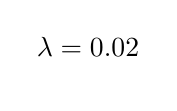
\begin{tikzpicture}[%
font=\footnotesize
]

\begin{axis}[%
width=0.951\figwidth,
height=\figheight,
at={(0\figwidth,0\figheight)},
scale only axis,
xmin=0,
xmax=3,
tick align=outside,
xlabel={Moneyness},
xmajorgrids,
ymin=0,
ymax=5,
ylabel={Remaining Time},
ymajorgrids,
zmin=0,
zmax=250000000,
zlabel={Optimal Rate},
zmajorgrids,
view={50}{40},
axis background/.style={fill=white},
title style={font=\bfseries},
title={$\lambda = 0.02$},
axis x line*=bottom,
axis y line*=left,
axis z line*=left
]

\addplot3[%
surf,
shader=flat corner,draw=black,z buffer=sort,colormap={mymap}{[1pt] rgb(0pt)=(0.2081,0.1663,0.5292); rgb(1pt)=(0.211624,0.189781,0.577676); rgb(2pt)=(0.212252,0.213771,0.626971); rgb(3pt)=(0.2081,0.2386,0.677086); rgb(4pt)=(0.195905,0.264457,0.7279); rgb(5pt)=(0.170729,0.291938,0.779248); rgb(6pt)=(0.125271,0.324243,0.830271); rgb(7pt)=(0.0591333,0.359833,0.868333); rgb(8pt)=(0.0116952,0.38751,0.881957); rgb(9pt)=(0.00595714,0.408614,0.882843); rgb(10pt)=(0.0165143,0.4266,0.878633); rgb(11pt)=(0.0328524,0.443043,0.871957); rgb(12pt)=(0.0498143,0.458571,0.864057); rgb(13pt)=(0.0629333,0.47369,0.855438); rgb(14pt)=(0.0722667,0.488667,0.8467); rgb(15pt)=(0.0779429,0.503986,0.838371); rgb(16pt)=(0.0793476,0.520024,0.831181); rgb(17pt)=(0.0749429,0.537543,0.826271); rgb(18pt)=(0.0640571,0.556986,0.823957); rgb(19pt)=(0.0487714,0.577224,0.822829); rgb(20pt)=(0.0343429,0.596581,0.819852); rgb(21pt)=(0.0265,0.6137,0.8135); rgb(22pt)=(0.0238905,0.628662,0.803762); rgb(23pt)=(0.0230905,0.641786,0.791267); rgb(24pt)=(0.0227714,0.653486,0.776757); rgb(25pt)=(0.0266619,0.664195,0.760719); rgb(26pt)=(0.0383714,0.674271,0.743552); rgb(27pt)=(0.0589714,0.683757,0.725386); rgb(28pt)=(0.0843,0.692833,0.706167); rgb(29pt)=(0.113295,0.7015,0.685857); rgb(30pt)=(0.145271,0.709757,0.664629); rgb(31pt)=(0.180133,0.717657,0.642433); rgb(32pt)=(0.217829,0.725043,0.619262); rgb(33pt)=(0.258643,0.731714,0.595429); rgb(34pt)=(0.302171,0.737605,0.571186); rgb(35pt)=(0.348167,0.742433,0.547267); rgb(36pt)=(0.395257,0.7459,0.524443); rgb(37pt)=(0.44201,0.748081,0.503314); rgb(38pt)=(0.487124,0.749062,0.483976); rgb(39pt)=(0.530029,0.749114,0.466114); rgb(40pt)=(0.570857,0.748519,0.44939); rgb(41pt)=(0.609852,0.747314,0.433686); rgb(42pt)=(0.6473,0.7456,0.4188); rgb(43pt)=(0.683419,0.743476,0.404433); rgb(44pt)=(0.71841,0.741133,0.390476); rgb(45pt)=(0.752486,0.7384,0.376814); rgb(46pt)=(0.785843,0.735567,0.363271); rgb(47pt)=(0.818505,0.732733,0.34979); rgb(48pt)=(0.850657,0.7299,0.336029); rgb(49pt)=(0.882433,0.727433,0.3217); rgb(50pt)=(0.913933,0.725786,0.306276); rgb(51pt)=(0.944957,0.726114,0.288643); rgb(52pt)=(0.973895,0.731395,0.266648); rgb(53pt)=(0.993771,0.745457,0.240348); rgb(54pt)=(0.999043,0.765314,0.216414); rgb(55pt)=(0.995533,0.786057,0.196652); rgb(56pt)=(0.988,0.8066,0.179367); rgb(57pt)=(0.978857,0.827143,0.163314); rgb(58pt)=(0.9697,0.848138,0.147452); rgb(59pt)=(0.962586,0.870514,0.1309); rgb(60pt)=(0.958871,0.8949,0.113243); rgb(61pt)=(0.959824,0.921833,0.0948381); rgb(62pt)=(0.9661,0.951443,0.0755333); rgb(63pt)=(0.9763,0.9831,0.0538)},mesh/rows=25]
table[row sep=crcr, point meta=\thisrow{c}] {%
%
x	y	z	c\\
0	0.01	32.6278781458054	32.6278781458054\\
0	0.111836734693878	41.0076003503939	41.0076003503939\\
0	0.213673469387755	54.0589975358155	54.0589975358155\\
0	0.315510204081633	73.3094190648448	73.3094190648448\\
0	0.41734693877551	100.723499127308	100.723499127308\\
0	0.519183673469388	139.124184740301	139.124184740301\\
0	0.621020408163265	192.492525136119	192.492525136119\\
0	0.722857142857143	266.382216782451	266.382216782451\\
0	0.82469387755102	368.498758547973	368.498758547973\\
0	0.926530612244898	509.504205472369	509.504205472369\\
0	1.02836734693878	704.131585460074	704.131585460074\\
0	1.13020408163265	972.725429151501	972.725429151501\\
0	1.23204081632653	1343.36947613791	1343.36947613791\\
0	1.33387755102041	1854.8240734861	1854.8240734861\\
0	1.43571428571429	2560.58050132957	2560.58050132957\\
0	1.53755102040816	3534.45631057053	3534.45631057053\\
0	1.63938775510204	4878.31696554989	4878.31696554989\\
0	1.74122448979592	6732.73151507002	6732.73151507002\\
0	1.8430612244898	9291.67693712214	9291.67693712214\\
0	1.94489795918367	12822.8293227826	12822.8293227826\\
0	2.04673469387755	17695.5644863963	17695.5644863963\\
0	2.14857142857143	24419.59704687	24419.59704687\\
0	2.25040816326531	33698.2998797338	33698.2998797338\\
0	2.35224489795918	46502.281503407	46502.281503407\\
0	2.45408163265306	64170.9180767198	64170.9180767198\\
0	2.55591836734694	88552.4609210853	88552.4609210853\\
0	2.65775510204082	122197.375734349	122197.375734349\\
0	2.75959183673469	168625.138048859	168625.138048859\\
0	2.86142857142857	232692.393491827	232692.393491827\\
0	2.96326530612245	321100.994831905	321100.994831905\\
0	3.06510204081633	443099.059826223	443099.059826223\\
0	3.1669387755102	611448.385128017	611448.385128017\\
0	3.26877551020408	843759.414110516	843759.414110516\\
0	3.37061224489796	1164333.40501675	1164333.40501675\\
0	3.47244897959184	1606704.50233654	1606704.50233654\\
0	3.57428571428571	2217147.62879039	2217147.62879039\\
0	3.67612244897959	3059519.14648492	3059519.14648492\\
0	3.77795918367347	4221936.65221952	4221936.65221952\\
0	3.87979591836735	5825996.65745919	5825996.65745919\\
0	3.98163265306122	8039494.38289073	8039494.38289073\\
0	4.0834693877551	11093976.24172	11093976.24172\\
0	4.18530612244898	15308961.1168367	15308961.1168367\\
0	4.28714285714286	21125364.1367308	21125364.1367308\\
0	4.38897959183674	29151619.2968362	29151619.2968362\\
0	4.49081632653061	40227325.6557171	40227325.6557171\\
0	4.59265306122449	55511074.9167983	55511074.9167983\\
0	4.69448979591837	76601647.7379719	76601647.7379719\\
0	4.79632653061224	105705256.69995	105705256.69995\\
0	4.89816326530612	145866330.647609	145866330.647609\\
0	5	201285981.963399	201285981.963399\\
0.125	0.01	31.958091902389	31.958091902389\\
0.125	0.111836734693878	38.270659435131	38.270659435131\\
0.125	0.213673469387755	49.2841858055305	49.2841858055305\\
0.125	0.315510204081633	65.9697772191185	65.9697772191185\\
0.125	0.41734693877551	90.0215310711632	90.0215310711632\\
0.125	0.519183673469388	123.916354528256	123.916354528256\\
0.125	0.621020408163265	171.16871696275	171.16871696275\\
0.125	0.722857142857143	236.696080170716	236.696080170716\\
0.125	0.82469387755102	327.331816691525	327.331816691525\\
0.125	0.926530612244898	452.539006547804	452.539006547804\\
0.125	1.02836734693878	625.399621103952	625.399621103952\\
0.125	1.13020408163265	863.982467267101	863.982467267101\\
0.125	1.23204081632653	1193.23292311307	1193.23292311307\\
0.125	1.33387755102041	1647.58210195761	1647.58210195761\\
0.125	1.43571428571429	2274.54835318586	2274.54835318586\\
0.125	1.53755102040816	3139.70782211691	3139.70782211691\\
0.125	1.63938775510204	4333.55400953697	4333.55400953697\\
0.125	1.74122448979592	5980.96387710864	5980.96387710864\\
0.125	1.8430612244898	8254.26070913611	8254.26070913611\\
0.125	1.94489795918367	11391.2401886066	11391.2401886066\\
0.125	2.04673469387755	15720.0453261401	15720.0453261401\\
0.125	2.14857142857143	21693.4923261356	21693.4923261356\\
0.125	2.25040816326531	29936.4380952037	29936.4380952037\\
0.125	2.35224489795918	41311.1443458412	41311.1443458412\\
0.125	2.45408163265306	57007.4758089239	57007.4758089239\\
0.125	2.55591836734694	78667.3678801614	78667.3678801614\\
0.125	2.65775510204082	108556.583863028	108556.583863028\\
0.125	2.75959183673469	149801.728537844	149801.728537844\\
0.125	2.86142857142857	206717.311860099	206717.311860099\\
0.125	2.96326530612245	285257.074752547	285257.074752547\\
0.125	3.06510204081633	393636.789684255	393636.789684255\\
0.125	3.1669387755102	543193.684445736	543193.684445736\\
0.125	3.26877551020408	749572.390703965	749572.390703965\\
0.125	3.37061224489796	1034361.47532412	1034361.47532412\\
0.125	3.47244897959184	1427351.74639403	1427351.74639403\\
0.125	3.57428571428571	1969652.567609	1969652.567609\\
0.125	3.67612244897959	2717992.16799075	2717992.16799075\\
0.125	3.77795918367347	3750651.78761016	3750651.78761016\\
0.125	3.87979591836735	5175654.40997209	5175654.40997209\\
0.125	3.98163265306122	7142064.67630838	7142064.67630838\\
0.125	4.0834693877551	9855582.02710814	9855582.02710814\\
0.125	4.18530612244898	13600058.2160104	13600058.2160104\\
0.125	4.28714285714286	18767190.0694847	18767190.0694847\\
0.125	4.38897959183674	25897493.5501847	25897493.5501847\\
0.125	4.49081632653061	35736845.2803953	35736845.2803953\\
0.125	4.59265306122449	49314506.1406754	49314506.1406754\\
0.125	4.69448979591837	68050788.7250956	68050788.7250956\\
0.125	4.79632653061224	93905631.3767817	93905631.3767817\\
0.125	4.89816326530612	129583620.624719	129583620.624719\\
0.125	5	178816908.716674	178816908.716674\\
0.25	0.01	31.9548698659926	31.9548698659926\\
0.25	0.111836734693878	37.4384992563269	37.4384992563269\\
0.25	0.213673469387755	47.3394702846674	47.3394702846674\\
0.25	0.315510204081633	62.6096720965758	62.6096720965758\\
0.25	0.41734693877551	84.8121561424287	84.8121561424287\\
0.25	0.519183673469388	116.247159159673	116.247159159673\\
0.25	0.621020408163265	160.184503551433	160.184503551433\\
0.25	0.722857142857143	221.204214736305	221.204214736305\\
0.25	0.82469387755102	305.675124914638	305.675124914638\\
0.25	0.926530612244898	422.420784306883	422.420784306883\\
0.25	1.02836734693878	583.642220766436	583.642220766436\\
0.25	1.13020408163265	806.194049732968	806.194049732968\\
0.25	1.23204081632653	1113.34741466132	1113.34741466132\\
0.25	1.33387755102041	1537.22416677636	1537.22416677636\\
0.25	1.43571428571429	2122.15690998243	2122.15690998243\\
0.25	1.53755102040816	2929.32638994023	2929.32638994023\\
0.25	1.63938775510204	4043.16132407377	4043.16132407377\\
0.25	1.74122448979592	5580.17013478363	5580.17013478363\\
0.25	1.8430612244898	7701.12844304316	7701.12844304316\\
0.25	1.94489795918367	10627.8972056399	10627.8972056399\\
0.25	2.04673469387755	14666.6307911173	14666.6307911173\\
0.25	2.14857142857143	20239.8027045781	20239.8027045781\\
0.25	2.25040816326531	27930.3990639401	27930.3990639401\\
0.25	2.35224489795918	38542.9027547349	38542.9027547349\\
0.25	2.45408163265306	53187.4476063808	53187.4476063808\\
0.25	2.55591836734694	73395.9456695517	73395.9456695517\\
0.25	2.65775510204082	101282.335317853	101282.335317853\\
0.25	2.75959183673469	139763.712845245	139763.712845245\\
0.25	2.86142857142857	192865.480387446	192865.480387446\\
0.25	2.96326530612245	266142.428955179	266142.428955179\\
0.25	3.06510204081633	367259.80632361	367259.80632361\\
0.25	3.1669387755102	506795.152289861	506795.152289861\\
0.25	3.26877551020408	699344.778871534	699344.778871534\\
0.25	3.37061224489796	965050.64050277	965050.64050277\\
0.25	3.47244897959184	1331707.31488905	1331707.31488905\\
0.25	3.57428571428571	1837669.49857092	1837669.49857092\\
0.25	3.67612244897959	2535864.16034861	2535864.16034861\\
0.25	3.77795918367347	3499327.05019439	3499327.05019439\\
0.25	3.87979591836735	4828842.71888632	4828842.71888632\\
0.25	3.98163265306122	6663487.24464776	6663487.24464776\\
0.25	4.0834693877551	9195176.50531535	9195176.50531535\\
0.25	4.18530612244898	12688741.840955	12688741.840955\\
0.25	4.28714285714286	17509633.1532285	17509633.1532285\\
0.25	4.38897959183674	24162147.3678455	24162147.3678455\\
0.25	4.49081632653061	33342181.2086153	33342181.2086153\\
0.25	4.59265306122449	46010026.5701043	46010026.5701043\\
0.25	4.69448979591837	63490823.363487	63490823.363487\\
0.25	4.79632653061224	87613177.8637244	87613177.8637244\\
0.25	4.89816326530612	120900446.948569	120900446.948569\\
0.25	5	166834697.821459	166834697.821459\\
0.375	0.01	31.9548697809241	31.9548697809241\\
0.375	0.111836734693878	37.2596629627883	37.2596629627883\\
0.375	0.213673469387755	46.6587816591923	46.6587816591923\\
0.375	0.315510204081633	61.2012106714596	61.2012106714596\\
0.375	0.41734693877551	82.4159775469182	82.4159775469182\\
0.375	0.519183673469388	112.522903041222	112.522903041222\\
0.375	0.621020408163265	154.668834368699	154.668834368699\\
0.375	0.722857142857143	213.258229834478	213.258229834478\\
0.375	0.82469387755102	294.414743376276	294.414743376276\\
0.375	0.926530612244898	406.622305623115	406.622305623115\\
0.375	1.02836734693878	561.612892505195	561.612892505195\\
0.375	1.13020408163265	775.593933608987	775.593933608987\\
0.375	1.23204081632653	1070.9438074396	1070.9438074396\\
0.375	1.33387755102041	1478.55281435144	1478.55281435144\\
0.375	1.43571428571429	2041.05452643454	2041.05452643454\\
0.375	1.53755102040816	2817.28554553698	2817.28554553698\\
0.375	1.63938775510204	3888.44019585448	3888.44019585448\\
0.375	1.74122448979592	5366.56397626961	5366.56397626961\\
0.375	1.8430612244898	7406.27424574536	7406.27424574536\\
0.375	1.94489795918367	10220.9342039507	10220.9342039507\\
0.375	2.04673469387755	14104.9720726905	14104.9720726905\\
0.375	2.14857142857143	19464.6802117697	19464.6802117697\\
0.375	2.25040816326531	26860.7159596045	26860.7159596045\\
0.375	2.35224489795918	37066.7500660996	37066.7500660996\\
0.375	2.45408163265306	51150.3977295559	51150.3977295559\\
0.375	2.55591836734694	70584.8981567304	70584.8981567304\\
0.375	2.65775510204082	97403.225059969	97403.225059969\\
0.375	2.75959183673469	134410.749066784	134410.749066784\\
0.375	2.86142857142857	185478.697924062	185478.697924062\\
0.375	2.96326530612245	255949.11236585	255949.11236585\\
0.375	3.06510204081633	353193.658690298	353193.658690298\\
0.375	3.1669387755102	487384.753515369	487384.753515369\\
0.375	3.26877551020408	672559.665432724	672559.665432724\\
0.375	3.37061224489796	928088.905588878	928088.905588878\\
0.375	3.47244897959184	1280702.51059729	1280702.51059729\\
0.375	3.57428571428571	1767286.1798007	1767286.1798007\\
0.375	3.67612244897959	2438739.76200848	2438739.76200848\\
0.375	3.77795918367347	3365301.71517415	3365301.71517415\\
0.375	3.87979591836735	4643896.50955981	4643896.50955981\\
0.375	3.98163265306122	6408273.5653814	6408273.5653814\\
0.375	4.0834693877551	8842998.32135328	8842998.32135328\\
0.375	4.18530612244898	12202758.9930468	12202758.9930468\\
0.375	4.28714285714286	16839008.6347482	16839008.6347482\\
0.375	4.38897959183674	23236729.4396509	23236729.4396509\\
0.375	4.49081632653061	32065165.0658984	32065165.0658984\\
0.375	4.59265306122449	44247827.923335	44247827.923335\\
0.375	4.69448979591837	61059104.6434373	61059104.6434373\\
0.375	4.79632653061224	84257565.2997399	84257565.2997399\\
0.375	4.89816326530612	116269921.399687	116269921.399687\\
0.375	5	160444875.863334	160444875.863334\\
0.5	0.01	31.954869780924	31.954869780924\\
0.5	0.111836734693878	37.2342619829567	37.2342619829567\\
0.5	0.213673469387755	46.4605434613376	46.4605434613376\\
0.5	0.315510204081633	60.6713997673894	60.6713997673894\\
0.5	0.41734693877551	81.3894548728715	81.3894548728715\\
0.5	0.519183673469388	110.800663320841	110.800663320841\\
0.5	0.621020408163265	151.992354171501	151.992354171501\\
0.5	0.722857142857143	209.279556749072	209.279556749072\\
0.5	0.82469387755102	288.658079248668	288.658079248668\\
0.5	0.926530612244898	398.432717947494	398.432717947494\\
0.5	1.02836734693878	550.086632575498	550.086632575498\\
0.5	1.13020408163265	759.482978920217	759.482978920217\\
0.5	1.23204081632653	1048.52457942513	1048.52457942513\\
0.5	1.33387755102041	1447.44529315838	1447.44529315838\\
0.5	1.43571428571429	1997.9728078535	1997.9728078535\\
0.5	1.53755102040816	2757.69372218764	2757.69372218764\\
0.5	1.63938775510204	3806.0775471771	3806.0775471771\\
0.5	1.74122448979592	5252.78978517888	5252.78978517888\\
0.5	1.8430612244898	7249.16369483821	7249.16369483821\\
0.5	1.94489795918367	10004.0307678663	10004.0307678663\\
0.5	2.04673469387755	13805.5658922703	13805.5658922703\\
0.5	2.14857142857143	19051.4323516118	19051.4323516118\\
0.5	2.25040816326531	26290.3800267449	26290.3800267449\\
0.5	2.35224489795918	36279.6482463905	36279.6482463905\\
0.5	2.45408163265306	50064.1780028208	50064.1780028208\\
0.5	2.55591836734694	69085.91965172	69085.91965172\\
0.5	2.65775510204082	95334.6704006713	95334.6704006713\\
0.5	2.75959183673469	131556.220179563	131556.220179563\\
0.5	2.86142857142857	181539.579319668	181539.579319668\\
0.5	2.96326530612245	250513.333945237	250513.333945237\\
0.5	3.06510204081633	345692.590457622	345692.590457622\\
0.5	3.1669387755102	477033.723101072	477033.723101072\\
0.5	3.26877551020408	658275.876167941	658275.876167941\\
0.5	3.37061224489796	908378.168821603	908378.168821603\\
0.5	3.47244897959184	1253502.94361086	1253502.94361086\\
0.5	3.57428571428571	1729752.51950985	1729752.51950985\\
0.5	3.67612244897959	2386945.73184475	2386945.73184475\\
0.5	3.77795918367347	3293829.31001362	3293829.31001362\\
0.5	3.87979591836735	4545269.23737205	4545269.23737205\\
0.5	3.98163265306122	6272174.35681024	6272174.35681024\\
0.5	4.0834693877551	8655190.29640994	8655190.29640994\\
0.5	4.18530612244898	11943596.1898085	11943596.1898085\\
0.5	4.28714285714286	16481380.9126801	16481380.9126801\\
0.5	4.38897959183674	22743226.5805313	22743226.5805313\\
0.5	4.49081632653061	31384163.4190534	31384163.4190534\\
0.5	4.59265306122449	43308090.2323535	43308090.2323535\\
0.5	4.69448979591837	59762328.1607722	59762328.1607722\\
0.5	4.79632653061224	82468098.672988	82468098.672988\\
0.5	4.89816326530612	113800574.648245	113800574.648245\\
0.5	5	157037339.075688	157037339.075688\\
0.625	0.01	31.954869780924	31.954869780924\\
0.625	0.111836734693878	37.2319808994604	37.2319808994604\\
0.625	0.213673469387755	46.4137514233492	46.4137514233492\\
0.625	0.315510204081633	60.4956785347704	60.4956785347704\\
0.625	0.41734693877551	80.9852718576754	80.9852718576754\\
0.625	0.519183673469388	110.050256018951	110.050256018951\\
0.625	0.621020408163265	150.748182481927	150.748182481927\\
0.625	0.722857142857143	207.348592257647	207.348592257647\\
0.625	0.82469387755102	285.781079112372	285.781079112372\\
0.625	0.926530612244898	394.256515622368	394.256515622368\\
0.625	1.02836734693878	544.126623682334	544.126623682334\\
0.625	1.13020408163265	751.071908445827	751.071908445827\\
0.625	1.23204081632653	1036.74228202716	1036.74228202716\\
0.625	1.33387755102041	1431.02203602319	1431.02203602319\\
0.625	1.43571428571429	1975.15612006735	1975.15612006735\\
0.625	1.53755102040816	2726.06477369526	2726.06477369526\\
0.625	1.63938775510204	3762.29786293077	3762.29786293077\\
0.625	1.74122448979592	5192.25179321445	5192.25179321445\\
0.625	1.8430612244898	7165.50854813094	7165.50854813094\\
0.625	1.94489795918367	9888.48299652049	9888.48299652049\\
0.625	2.04673469387755	13646.0152825248	13646.0152825248\\
0.625	2.14857142857143	18831.1670070018	18831.1670070018\\
0.625	2.25040816326531	25986.33807863	25986.33807863\\
0.625	2.35224489795918	35860.005329045	35860.005329045\\
0.625	2.45408163265306	49485.0181252453	49485.0181252453\\
0.625	2.55591836734694	68286.6412159011	68286.6412159011\\
0.625	2.65775510204082	94231.6468042637	94231.6468042637\\
0.625	2.75959183673469	130034.051859227	130034.051859227\\
0.625	2.86142857142857	179439.022140321	179439.022140321\\
0.625	2.96326530612245	247614.641164546	247614.641164546\\
0.625	3.06510204081633	341692.525725001	341692.525725001\\
0.625	3.1669387755102	471513.83989914	471513.83989914\\
0.625	3.26877551020408	650658.745516939	650658.745516939\\
0.625	3.37061224489796	897866.976376426	897866.976376426\\
0.625	3.47244897959184	1238998.13760955	1238998.13760955\\
0.625	3.57428571428571	1709736.79040063	1709736.79040063\\
0.625	3.67612244897959	2359325.29170417	2359325.29170417\\
0.625	3.77795918367347	3255714.86853924	3255714.86853924\\
0.625	3.87979591836735	4492673.76309848	4492673.76309848\\
0.625	3.98163265306122	6199596.00738458	6199596.00738458\\
0.625	4.0834693877551	8555036.88969148	8555036.88969148\\
0.625	4.18530612244898	11805391.0117165	11805391.0117165\\
0.625	4.28714285714286	16290666.7838812	16290666.7838812\\
0.625	4.38897959183674	22480053.540532	22480053.540532\\
0.625	4.49081632653061	31021001.8291159	31021001.8291159\\
0.625	4.59265306122449	42806950.9942703	42806950.9942703\\
0.625	4.69448979591837	59070788.8074133	59070788.8074133\\
0.625	4.79632653061224	81513819.6335652	81513819.6335652\\
0.625	4.89816326530612	112483732.053586	112483732.053586\\
0.625	5	155220182.525283	155220182.525283\\
0.75	0.01	31.954869780924	31.954869780924\\
0.75	0.111836734693878	37.2318549881823	37.2318549881823\\
0.75	0.213673469387755	46.4049766210674	46.4049766210674\\
0.75	0.315510204081633	60.445039261153	60.445039261153\\
0.75	0.41734693877551	80.8406827064153	80.8406827064153\\
0.75	0.519183673469388	109.745130353582	109.745130353582\\
0.75	0.621020408163265	150.198663240096	150.198663240096\\
0.75	0.722857142857143	206.446602762073	206.446602762073\\
0.75	0.82469387755102	284.383838051315	284.383838051315\\
0.75	0.926530612244898	392.171936537558	392.171936537558\\
0.75	1.02836734693878	541.09330488493	541.09330488493\\
0.75	1.13020408163265	746.731739666194	746.731739666194\\
0.75	1.23204081632653	1030.60286737347	1030.60286737347\\
0.75	1.33387755102041	1422.40503877967	1422.40503877967\\
0.75	1.43571428571429	1963.12614620594	1963.12614620594\\
0.75	1.53755102040816	2709.33136608366	2709.33136608366\\
0.75	1.63938775510204	3739.08036016544	3739.08036016544\\
0.75	1.74122448979592	5160.09291935991	5160.09291935991\\
0.75	1.8430612244898	7121.01723480893	7121.01723480893\\
0.75	1.94489795918367	9826.97953503675	9826.97953503675\\
0.75	2.04673469387755	13561.0416862548	13561.0416862548\\
0.75	2.14857142857143	18713.8113640828	18713.8113640828\\
0.75	2.25040816326531	25824.3022170454	25824.3022170454\\
0.75	2.35224489795918	35636.3182649407	35636.3182649407\\
0.75	2.45408163265306	49176.2607119313	49176.2607119313\\
0.75	2.55591836734694	67860.4962794142	67860.4962794142\\
0.75	2.65775510204082	93643.5184928807	93643.5184928807\\
0.75	2.75959183673469	129222.400568041	129222.400568041\\
0.75	2.86142857142857	178318.927012758	178318.927012758\\
0.75	2.96326530612245	246068.916765656	246068.916765656\\
0.75	3.06510204081633	339559.463631694	339559.463631694\\
0.75	3.1669387755102	468570.292896703	468570.292896703\\
0.75	3.26877551020408	646596.784897229	646596.784897229\\
0.75	3.37061224489796	892261.680537331	892261.680537331\\
0.75	3.47244897959184	1231263.14243116	1231263.14243116\\
0.75	3.57428571428571	1699062.95167497	1699062.95167497\\
0.75	3.67612244897959	2344596.04330517	2344596.04330517\\
0.75	3.77795918367347	3235389.42224076	3235389.42224076\\
0.75	3.87979591836735	4464625.93197335	4464625.93197335\\
0.75	3.98163265306122	6160891.79265225	6160891.79265225\\
0.75	4.0834693877551	8501627.56513618	8501627.56513618\\
0.75	4.18530612244898	11731689.6002879	11731689.6002879\\
0.75	4.28714285714286	16188963.6231456	16188963.6231456\\
0.75	4.38897959183674	22339709.8012771	22339709.8012771\\
0.75	4.49081632653061	30827336.6238529	30827336.6238529\\
0.75	4.59265306122449	42539705.6598656	42539705.6598656\\
0.75	4.69448979591837	58702007.7157154	58702007.7157154\\
0.75	4.79632653061224	81004925.8488846	81004925.8488846\\
0.75	4.89816326530612	111781491.931573	111781491.931573\\
0.75	5	154251137.123632	154251137.123632\\
0.875	0.01	31.954869780924	31.954869780924\\
0.875	0.111836734693878	37.2318507936867	37.2318507936867\\
0.875	0.213673469387755	46.4036882735202	46.4036882735202\\
0.875	0.315510204081633	60.4325075783433	60.4325075783433\\
0.875	0.41734693877551	80.7941426342981	80.7941426342981\\
0.875	0.519183673469388	109.630312423297	109.630312423297\\
0.875	0.621020408163265	149.969754036434	149.969754036434\\
0.875	0.722857142857143	206.043734804787	206.043734804787\\
0.875	0.82469387755102	283.728236994009	283.728236994009\\
0.875	0.926530612244898	391.158550221426	391.158550221426\\
0.875	1.02836734693878	539.580344907348	539.580344907348\\
0.875	1.13020408163265	744.526164231425	744.526164231425\\
0.875	1.23204081632653	1027.44036380876	1027.44036380876\\
0.875	1.33387755102041	1417.92246104787	1417.92246104787\\
0.875	1.43571428571429	1956.82355619359	1956.82355619359\\
0.875	1.53755102040816	2700.51972888785	2700.51972888785\\
0.875	1.63938775510204	3726.80943576492	3726.80943576492\\
0.875	1.74122448979592	5143.05181678549	5143.05181678549\\
0.875	1.8430612244898	7097.39723215484	7097.39723215484\\
0.875	1.94489795918367	9794.28481935805	9794.28481935805\\
0.875	2.04673469387755	13515.8282180989	13515.8282180989\\
0.875	2.14857142857143	18651.3265518446	18651.3265518446\\
0.875	2.25040816326531	25737.9877097679	25737.9877097679\\
0.875	2.35224489795918	35517.1238530563	35517.1238530563\\
0.875	2.45408163265306	49011.6975658027	49011.6975658027\\
0.875	2.55591836734694	67633.330488368	67633.330488368\\
0.875	2.65775510204082	93329.9682403691	93329.9682403691\\
0.875	2.75959183673469	128789.648355559	128789.648355559\\
0.875	2.86142857142857	177721.686694692	177721.686694692\\
0.875	2.96326530612245	245244.696284218	245244.696284218\\
0.875	3.06510204081633	338422.027902725	338422.027902725\\
0.875	3.1669387755102	467000.64302108	467000.64302108\\
0.875	3.26877551020408	644430.710063936	644430.710063936\\
0.875	3.37061224489796	889272.580465259	889272.580465259\\
0.875	3.47244897959184	1227138.32346397	1227138.32346397\\
0.875	3.57428571428571	1693370.91694458	1693370.91694458\\
0.875	3.67612244897959	2336741.35529976	2336741.35529976\\
0.875	3.77795918367347	3224550.41610503	3224550.41610503\\
0.875	3.87979591836735	4449668.76394263	4449668.76394263\\
0.875	3.98163265306122	6140251.83252146	6140251.83252146\\
0.875	4.0834693877551	8473145.7256359	8473145.7256359\\
0.875	4.18530612244898	11692386.4823443	11692386.4823443\\
0.875	4.28714285714286	16134727.8511331	16134727.8511331\\
0.875	4.38897959183674	22264867.9460824	22264867.9460824\\
0.875	4.49081632653061	30724059.7248746	30724059.7248746\\
0.875	4.59265306122449	42397190.2642492	42397190.2642492\\
0.875	4.69448979591837	58505345.7661427	58505345.7661427\\
0.875	4.79632653061224	80733545.2027499	80733545.2027499\\
0.875	4.89816326530612	111407004.379599	111407004.379599\\
0.875	5	153734368.796524	153734368.796524\\
1	0.01	31.954869780924	31.954869780924\\
1	0.111836734693878	37.2318507103871	37.2318507103871\\
1	0.213673469387755	46.4035417293483	46.4035417293483\\
1	0.315510204081633	60.4298688215704	60.4298688215704\\
1	0.41734693877551	80.7807707521895	80.7807707521895\\
1	0.519183673469388	109.590610171099	109.590610171099\\
1	0.621020408163265	149.88039799321	149.88039799321\\
1	0.722857142857143	205.872698941272	205.872698941272\\
1	0.82469387755102	283.432646975462	283.432646975462\\
1	0.926530612244898	390.681107465405	390.681107465405\\
1	1.02836734693878	538.843997199918	538.843997199918\\
1	1.13020408163265	743.426522952396	743.426522952396\\
1	1.23204081632653	1025.83512258715	1025.83512258715\\
1	1.33387755102041	1415.61674596312	1415.61674596312\\
1	1.43571428571429	1953.54970268104	1953.54970268104\\
1	1.53755102040816	2695.90939022195	2695.90939022195\\
1	1.63938775510204	3720.35512036998	3720.35512036998\\
1	1.74122448979592	5134.05384179157	5134.05384179157\\
1	1.8430612244898	7084.89055212437	7084.89055212437\\
1	1.94489795918367	9776.93808178159	9776.93808178159\\
1	2.04673469387755	13491.80449044	13491.80449044\\
1	2.14857142857143	18618.0911543703	18618.0911543703\\
1	2.25040816326531	25692.0430544919	25692.0430544919\\
1	2.35224489795918	35453.6435528694	35453.6435528694\\
1	2.45408163265306	48924.0215404222	48924.0215404222\\
1	2.55591836734694	67512.2682527583	67512.2682527583\\
1	2.65775510204082	93162.8374956688	93162.8374956688\\
1	2.75959183673469	128558.948313271	128558.948313271\\
1	2.86142857142857	177403.267355456	177403.267355456\\
1	2.96326530612245	244805.232165924	244805.232165924\\
1	3.06510204081633	337815.531953472	337815.531953472\\
1	3.1669387755102	466163.656049472	466163.656049472\\
1	3.26877551020408	643275.662469539	643275.662469539\\
1	3.37061224489796	887678.631862634	887678.631862634\\
1	3.47244897959184	1224938.72196474	1224938.72196474\\
1	3.57428571428571	1690335.55579528	1690335.55579528\\
1	3.67612244897959	2332552.70218518	2332552.70218518\\
1	3.77795918367347	3218770.29716379	3218770.29716379\\
1	3.87979591836735	4441692.52788467	4441692.52788467\\
1	3.98163265306122	6129245.10011273	6129245.10011273\\
1	4.0834693877551	8457957.10813046	8457957.10813046\\
1	4.18530612244898	11671427.1386379	11671427.1386379\\
1	4.28714285714286	16105805.2845246	16105805.2845246\\
1	4.38897959183674	22224956.6546917	22224956.6546917\\
1	4.49081632653061	30668984.7142424	30668984.7142424\\
1	4.59265306122449	42321190.3154561	42321190.3154561\\
1	4.69448979591837	58400470.774421	58400470.774421\\
1	4.79632653061224	80588824.5442454	80588824.5442454\\
1	4.89816326530612	111207299.311977	111207299.311977\\
1	5	153458788.846979	153458788.846979\\
1.125	0.01	31.954869780924	31.954869780924\\
1.125	0.111836734693878	37.2318507094094	37.2318507094094\\
1.125	0.213673469387755	46.4035289143228	46.4035289143228\\
1.125	0.315510204081633	60.4293993871347	60.4293993871347\\
1.125	0.41734693877551	80.7773632518318	80.7773632518318\\
1.125	0.519183673469388	109.578069091	109.578069091\\
1.125	0.621020408163265	149.847890856129	149.847890856129\\
1.125	0.722857142857143	205.804035533938	205.804035533938\\
1.125	0.82469387755102	283.305208693212	283.305208693212\\
1.125	0.926530612244898	390.464100535898	390.464100535898\\
1.125	1.02836734693878	538.495773337773	538.495773337773\\
1.125	1.13020408163265	742.890670827788	742.890670827788\\
1.125	1.23204081632653	1025.03492644292	1025.03492644292\\
1.125	1.33387755102041	1414.44744389768	1414.44744389768\\
1.125	1.43571428571429	1951.86774808228	1951.86774808228\\
1.125	1.53755102040816	2693.51760524524	2693.51760524524\\
1.125	1.63938775510204	3716.98219882824	3716.98219882824\\
1.125	1.74122448979592	5129.32606587189	5129.32606587189\\
1.125	1.8430612244898	7078.29277118472	7078.29277118472\\
1.125	1.94489795918367	9767.75987681162	9767.75987681162\\
1.125	2.04673469387755	13479.0658969403	13479.0658969403\\
1.125	2.14857142857143	18600.44017716	18600.44017716\\
1.125	2.25040816326531	25667.6142564729	25667.6142564729\\
1.125	2.35224489795918	35419.8629272859	35419.8629272859\\
1.125	2.45408163265306	48877.3372566001	48877.3372566001\\
1.125	2.55591836734694	67447.7791108402	67447.7791108402\\
1.125	2.65775510204082	93073.7802252695	93073.7802252695\\
1.125	2.75959183673469	128435.990084911	128435.990084911\\
1.125	2.86142857142857	177233.529497437	177233.529497437\\
1.125	2.96326530612245	244570.942961495	244570.942961495\\
1.125	3.06510204081633	337492.167592398	337492.167592398\\
1.125	3.1669387755102	465717.375265608	465717.375265608\\
1.125	3.26877551020408	642659.766510881	642659.766510881\\
1.125	3.37061224489796	886828.679483596	886828.679483596\\
1.125	3.47244897959184	1223765.78843689	1223765.78843689\\
1.125	3.57428571428571	1688716.93078488	1688716.93078488\\
1.125	3.67612244897959	2330319.05343432	2330319.05343432\\
1.125	3.77795918367347	3215687.95721202	3215687.95721202\\
1.125	3.87979591836735	4437439.05090564	4437439.05090564\\
1.125	3.98163265306122	6123375.53195031	6123375.53195031\\
1.125	4.0834693877551	8449857.44115848	8449857.44115848\\
1.125	4.18530612244898	11660250.0825156	11660250.0825156\\
1.125	4.28714285714286	16090381.6340471	16090381.6340471\\
1.125	4.38897959183674	22203672.9832285	22203672.9832285\\
1.125	4.49081632653061	30639614.5986958	30639614.5986958\\
1.125	4.59265306122449	42280661.4377582	42280661.4377582\\
1.125	4.69448979591837	58344543.5368559	58344543.5368559\\
1.125	4.79632653061224	80511648.5796458	80511648.5796458\\
1.125	4.89816326530612	111100801.496847	111100801.496847\\
1.125	5	153311828.799688	153311828.799688\\
1.25	0.01	31.954869780924	31.954869780924\\
1.25	0.111836734693878	37.2318507094026	37.2318507094026\\
1.25	0.213673469387755	46.4035280575809	46.4035280575809\\
1.25	0.315510204081633	60.4293292148816	60.4293292148816\\
1.25	0.41734693877551	80.7765970963394	80.7765970963394\\
1.25	0.519183673469388	109.574467779958	109.574467779958\\
1.25	0.621020408163265	149.836920498154	149.836920498154\\
1.25	0.722857142857143	205.778085005095	205.778085005095\\
1.25	0.82469387755102	283.252896172937	283.252896172937\\
1.25	0.926530612244898	390.369337067158	390.369337067158\\
1.25	1.02836734693878	538.336385784201	538.336385784201\\
1.25	1.13020408163265	742.636387909664	742.636387909664\\
1.25	1.23204081632653	1024.64449277475	1024.64449277475\\
1.25	1.33387755102041	1413.86455075744	1413.86455075744\\
1.25	1.43571428571429	1951.01535357486	1951.01535357486\\
1.25	1.53755102040816	2692.29005175098	2692.29005175098\\
1.25	1.63938775510204	3715.23430677452	3715.23430677452\\
1.25	1.74122448979592	5126.85806701606	5126.85806701606\\
1.25	1.8430612244898	7074.82950927441	7074.82950927441\\
1.25	1.94489795918367	9762.9221034593	9762.9221034593\\
1.25	2.04673469387755	13472.3306632092	13472.3306632092\\
1.25	2.14857142857143	18591.0861802431	18591.0861802431\\
1.25	2.25040816326531	25654.6464266312	25654.6464266312\\
1.25	2.35224489795918	35401.9083682315	35401.9083682315\\
1.25	2.45408163265306	48852.501655573	48852.501655573\\
1.25	2.55591836734694	67413.4485992248	67413.4485992248\\
1.25	2.65775510204082	93026.3479641389	93026.3479641389\\
1.25	2.75959183673469	128370.478975431	128370.478975431\\
1.25	2.86142857142857	177143.071549883	177143.071549883\\
1.25	2.96326530612245	244446.060862055	244446.060862055\\
1.25	3.06510204081633	337319.783315416	337319.783315416\\
1.25	3.1669387755102	465479.442026004	465479.442026004\\
1.25	3.26877551020408	642331.380950291	642331.380950291\\
1.25	3.37061224489796	886375.47661279	886375.47661279\\
1.25	3.47244897959184	1223140.34682852	1223140.34682852\\
1.25	3.57428571428571	1687853.81197629	1687853.81197629\\
1.25	3.67612244897959	2329127.95662946	2329127.95662946\\
1.25	3.77795918367347	3214044.27321949	3214044.27321949\\
1.25	3.87979591836735	4435170.8271926	4435170.8271926\\
1.25	3.98163265306122	6120245.48527155	6120245.48527155\\
1.25	4.0834693877551	8445538.13616316	8445538.13616316\\
1.25	4.18530612244898	11654289.6798511	11654289.6798511\\
1.25	4.28714285714286	16082156.6249859	16082156.6249859\\
1.25	4.38897959183674	22192322.9665507	22192322.9665507\\
1.25	4.49081632653061	30623952.2770584	30623952.2770584\\
1.25	4.59265306122449	42259048.4185811	42259048.4185811\\
1.25	4.69448979591837	58314718.9456807	58314718.9456807\\
1.25	4.79632653061224	80470492.5577972	80470492.5577972\\
1.25	4.89816326530612	111044008.843697	111044008.843697\\
1.25	5	153233458.620361	153233458.620361\\
1.375	0.01	31.954869780924	31.954869780924\\
1.375	0.111836734693878	37.2318507094026	37.2318507094026\\
1.375	0.213673469387755	46.4035280139751	46.4035280139751\\
1.375	0.315510204081633	60.4293204379233	60.4293204379233\\
1.375	0.41734693877551	80.77644572364	80.77644572364\\
1.375	0.519183673469388	109.573531369923	109.573531369923\\
1.375	0.621020408163265	149.833499313095	149.833499313095\\
1.375	0.722857142857143	205.768886602216	205.768886602216\\
1.375	0.82469387755102	283.232525903188	283.232525903188\\
1.375	0.926530612244898	390.329723619094	390.329723619094\\
1.375	1.02836734693878	538.266024795844	538.266024795844\\
1.375	1.13020408163265	742.519278863898	742.519278863898\\
1.375	1.23204081632653	1024.45862735442	1024.45862735442\\
1.375	1.33387755102041	1413.57977579466	1413.57977579466\\
1.375	1.43571428571429	1950.59037442167	1950.59037442167\\
1.375	1.53755102040816	2691.66825717256	2691.66825717256\\
1.375	1.63938775510204	3714.33797636963	3714.33797636963\\
1.375	1.74122448979592	5125.58035483992	5125.58035483992\\
1.375	1.8430612244898	7073.02336575426	7073.02336575426\\
1.375	1.94489795918367	9760.38497794556	9760.38497794556\\
1.375	2.04673469387755	13468.7833883515	13468.7833883515\\
1.375	2.14857142857143	18586.1438308022	18586.1438308022\\
1.375	2.25040816326531	25647.7781057525	25647.7781057525\\
1.375	2.35224489795918	35392.3817158376	35392.3817158376\\
1.375	2.45408163265306	48839.3062752364	48839.3062752364\\
1.375	2.55591836734694	67395.190394483	67395.190394483\\
1.375	2.65775510204082	93001.1033320228	93001.1033320228\\
1.375	2.75959183673469	128335.59360566	128335.59360566\\
1.375	2.86142857142857	177094.88278346	177094.88278346\\
1.375	2.96326530612245	244379.514566719	244379.514566719\\
1.375	3.06510204081633	337227.905201094	337227.905201094\\
1.375	3.1669387755102	465352.608096785	465352.608096785\\
1.375	3.26877551020408	642156.31077778	642156.31077778\\
1.375	3.37061224489796	886133.844120902	886133.844120902\\
1.375	3.47244897959184	1222806.86326894	1222806.86326894\\
1.375	3.57428571428571	1687393.58056143	1687393.58056143\\
1.375	3.67612244897959	2328492.82210037	2328492.82210037\\
1.375	3.77795918367347	3213167.78448958	3213167.78448958\\
1.375	3.87979591836735	4433961.28612686	4433961.28612686\\
1.375	3.98163265306122	6118576.35445788	6118576.35445788\\
1.375	4.0834693877551	8443234.80226576	8443234.80226576\\
1.375	4.18530612244898	11651111.1879058	11651111.1879058\\
1.375	4.28714285714286	16077770.4729245	16077770.4729245\\
1.375	4.38897959183674	22186270.3232964	22186270.3232964\\
1.375	4.49081632653061	30615599.9857755	30615599.9857755\\
1.375	4.59265306122449	42247522.7643048	42247522.7643048\\
1.375	4.69448979591837	58298814.2589841	58298814.2589841\\
1.375	4.79632653061224	80448545.0938395	80448545.0938395\\
1.375	4.89816326530612	111013722.743571	111013722.743571\\
1.375	5	153191665.749155	153191665.749155\\
1.5	0.01	31.954869780924	31.954869780924\\
1.5	0.111836734693878	37.2318507094026	37.2318507094026\\
1.5	0.213673469387755	46.4035280122907	46.4035280122907\\
1.5	0.315510204081633	60.4293195223471	60.4293195223471\\
1.5	0.41734693877551	80.776419529705	80.776419529705\\
1.5	0.519183673469388	109.573311613544	109.573311613544\\
1.5	0.621020408163265	149.832516532949	149.832516532949\\
1.5	0.722857142857143	205.765838387067	205.765838387067\\
1.5	0.82469387755102	283.225025265051	283.225025265051\\
1.5	0.926530612244898	390.313921852132	390.313921852132\\
1.5	1.02836734693878	538.236162228093	538.236162228093\\
1.5	1.13020408163265	742.467096480665	742.467096480665\\
1.5	1.23204081632653	1024.37255742878	1024.37255742878\\
1.5	1.33387755102041	1413.44381043354	1413.44381043354\\
1.5	1.43571428571429	1950.38248169589	1950.38248169589\\
1.5	1.53755102040816	2691.35817096913	2691.35817096913\\
1.5	1.63938775510204	3713.88412348322	3713.88412348322\\
1.5	1.74122448979592	5124.92559464365	5124.92559464365\\
1.5	1.8430612244898	7072.08909500784	7072.08909500784\\
1.5	1.94489795918367	9759.0629832358	9759.0629832358\\
1.5	2.04673469387755	13466.924593664	13466.924593664\\
1.5	2.14857142857143	18583.5427633161	18583.5427633161\\
1.5	2.25040816326531	25644.1514552725	25644.1514552725\\
1.5	2.35224489795918	35387.338745552	35387.338745552\\
1.5	2.45408163265306	48832.3079891364	48832.3079891364\\
1.5	2.55591836734694	67385.4931906588	67385.4931906588\\
1.5	2.65775510204082	92987.6812481542	92987.6812481542\\
1.5	2.75959183673469	128317.031023588	128317.031023588\\
1.5	2.86142857142857	177069.226369513	177069.226369513\\
1.5	2.96326530612245	244344.068960212	244344.068960212\\
1.5	3.06510204081633	337178.951079063	337178.951079063\\
1.5	3.1669387755102	465285.013123032	465285.013123032\\
1.5	3.26877551020408	642062.99273924	642062.99273924\\
1.5	3.37061224489796	886005.03009215	886005.03009215\\
1.5	3.47244897959184	1222629.06730882	1222629.06730882\\
1.5	3.57428571428571	1687148.19300232	1687148.19300232\\
1.5	3.67612244897959	2328154.16286077	2328154.16286077\\
1.5	3.77795918367347	3212700.4167737	3212700.4167737\\
1.5	3.87979591836735	4433316.30950686	4433316.30950686\\
1.5	3.98163265306122	6117686.28957079	6117686.28957079\\
1.5	4.0834693877551	8442006.53203089	8442006.53203089\\
1.5	4.18530612244898	11649416.2168677	11649416.2168677\\
1.5	4.28714285714286	16075431.4857848	16075431.4857848\\
1.5	4.38897959183674	22183042.6365683	22183042.6365683\\
1.5	4.49081632653061	30611145.9522831	30611145.9522831\\
1.5	4.59265306122449	42241376.4530682	42241376.4530682\\
1.5	4.69448979591837	58290332.7157756	58290332.7157756\\
1.5	4.79632653061224	80436841.0839428	80436841.0839428\\
1.5	4.89816326530612	110997571.941197	110997571.941197\\
1.5	5	153169378.664912	153169378.664912\\
1.625	0.01	31.954869780924	31.954869780924\\
1.625	0.111836734693878	37.2318507094026	37.2318507094026\\
1.625	0.213673469387755	46.4035280122415	46.4035280122415\\
1.625	0.315510204081633	60.4293194428944	60.4293194428944\\
1.625	0.41734693877551	80.7764155702603	80.7764155702603\\
1.625	0.519183673469388	109.573265190304	109.573265190304\\
1.625	0.621020408163265	149.832257169968	149.832257169968\\
1.625	0.722857142857143	205.764896520313	205.764896520313\\
1.625	0.82469387755102	283.222420651473	283.222420651473\\
1.625	0.926530612244898	390.307923253867	390.307923253867\\
1.625	1.02836734693878	538.224010198405	538.224010198405\\
1.625	1.13020408163265	742.44466158965	742.44466158965\\
1.625	1.23204081632653	1024.333891938	1024.333891938\\
1.625	1.33387755102041	1413.38053797834	1413.38053797834\\
1.625	1.43571428571429	1950.28295288713	1950.28295288713\\
1.625	1.53755102040816	2691.20628964841	2691.20628964841\\
1.625	1.63938775510204	3713.65771543947	3713.65771543947\\
1.625	1.74122448979592	5124.59414413825	5124.59414413825\\
1.625	1.8430612244898	7071.61060948382	7071.61060948382\\
1.625	1.94489795918367	9758.37965629506	9758.37965629506\\
1.625	2.04673469387755	13465.9568113691	13465.9568113691\\
1.625	2.14857142857143	18582.1808260729	18582.1808260729\\
1.625	2.25040816326531	25642.2441489385	25642.2441489385\\
1.625	2.35224489795918	35384.6775660742	35384.6775660742\\
1.625	2.45408163265306	48828.605370517	48828.605370517\\
1.625	2.55591836734694	67380.3524588687	67380.3524588687\\
1.625	2.65775510204082	92980.5551581598	92980.5551581598\\
1.625	2.75959183673469	128307.164542416	128307.164542416\\
1.625	2.86142857142857	177055.577720325	177055.577720325\\
1.625	2.96326530612245	244325.200668334	244325.200668334\\
1.625	3.06510204081633	337152.879622897	337152.879622897\\
1.625	3.1669387755102	465249.001462598	465249.001462598\\
1.625	3.26877551020408	642013.26401967	642013.26401967\\
1.625	3.37061224489796	885936.372573854	885936.372573854\\
1.625	3.47244897959184	1222534.28919759	1222534.28919759\\
1.625	3.57428571428571	1687017.37015125	1687017.37015125\\
1.625	3.67612244897959	2327973.60064869	2327973.60064869\\
1.625	3.77795918367347	3212451.2175661	3212451.2175661\\
1.625	3.87979591836735	4432972.39584629	4432972.39584629\\
1.625	3.98163265306122	6117211.67630958	6117211.67630958\\
1.625	4.0834693877551	8441351.56205358	8441351.56205358\\
1.625	4.18530612244898	11648512.3666348	11648512.3666348\\
1.625	4.28714285714286	16074184.1973243	16074184.1973243\\
1.625	4.38897959183674	22181321.426093	22181321.426093\\
1.625	4.49081632653061	30608770.7607317	30608770.7607317\\
1.625	4.59265306122449	42238098.810746	42238098.810746\\
1.625	4.69448979591837	58285809.7507924	58285809.7507924\\
1.625	4.79632653061224	80430599.6555609	80430599.6555609\\
1.625	4.89816326530612	110988959.1462	110988959.1462\\
1.625	5	153157493.539636	153157493.539636\\
1.75	0.01	31.954869780924	31.954869780924\\
1.75	0.111836734693878	37.2318507094026	37.2318507094026\\
1.75	0.213673469387755	46.4035280122404	46.4035280122404\\
1.75	0.315510204081633	60.4293194371702	60.4293194371702\\
1.75	0.41734693877551	80.7764150485498	80.7764150485498\\
1.75	0.519183673469388	109.573256381734	109.573256381734\\
1.75	0.621020408163265	149.832194425497	149.832194425497\\
1.75	0.722857142857143	205.764625766351	205.764625766351\\
1.75	0.82469387755102	283.221569620484	283.221569620484\\
1.75	0.926530612244898	390.305761197889	390.305761197889\\
1.75	1.02836734693878	538.219280135417	538.219280135417\\
1.75	1.13020408163265	742.435377425691	742.435377425691\\
1.75	1.23204081632653	1024.31708230542	1024.31708230542\\
1.75	1.33387755102041	1413.35190883795	1413.35190883795\\
1.75	1.43571428571429	1950.23643041134	1950.23643041134\\
1.75	1.53755102040816	2691.13339173765	2691.13339173765\\
1.75	1.63938775510204	3713.54668241169	3713.54668241169\\
1.75	1.74122448979592	5124.42873439915	5124.42873439915\\
1.75	1.8430612244898	7071.36843151255	7071.36843151255\\
1.75	1.94489795918367	9758.02986033993	9758.02986033993\\
1.75	2.04673469387755	13465.4568977706	13465.4568977706\\
1.75	2.14857142857143	18581.4722351441	18581.4722351441\\
1.75	2.25040816326531	25641.2461702157	25641.2461702157\\
1.75	2.35224489795918	35383.2789292085	35383.2789292085\\
1.75	2.45408163265306	48826.6526377694	48826.6526377694\\
1.75	2.55591836734694	67377.6340047478	67377.6340047478\\
1.75	2.65775510204082	92976.7790602436	92976.7790602436\\
1.75	2.75959183673469	128301.92807055	128301.92807055\\
1.75	2.86142857142857	177048.325232584	177048.325232584\\
1.75	2.96326530612245	244315.16550944	244315.16550944\\
1.75	3.06510204081633	337139.003947381	337139.003947381\\
1.75	3.1669387755102	465229.825595764	465229.825595764\\
1.75	3.26877551020408	641986.773782919	641986.773782919\\
1.75	3.37061224489796	885899.788603691	885899.788603691\\
1.75	3.47244897959184	1222483.77621982	1222483.77621982\\
1.75	3.57428571428571	1686947.63579864	1686947.63579864\\
1.75	3.67612244897959	2327877.3418559	2327877.3418559\\
1.75	3.77795918367347	3212318.3566312	3212318.3566312\\
1.75	3.87979591836735	4432789.02624612	4432789.02624612\\
1.75	3.98163265306122	6116958.6079942	6116958.6079942\\
1.75	4.0834693877551	8441002.31404825	8441002.31404825\\
1.75	4.18530612244898	11648030.3969626	11648030.3969626\\
1.75	4.28714285714286	16073519.0804807	16073519.0804807\\
1.75	4.38897959183674	22180403.5782122	22180403.5782122\\
1.75	4.49081632653061	30607504.1606612	30607504.1606612\\
1.75	4.59265306122449	42236350.9556068	42236350.9556068\\
1.75	4.69448979591837	58283397.7953105	58283397.7953105\\
1.75	4.79632653061224	80427271.2852525	80427271.2852525\\
1.75	4.89816326530612	110984366.183621	110984366.183621\\
1.75	5	153151155.522733	153151155.522733\\
1.875	0.01	31.954869780924	31.954869780924\\
1.875	0.111836734693878	37.2318507094026	37.2318507094026\\
1.875	0.213673469387755	46.4035280122404	46.4035280122404\\
1.875	0.315510204081633	60.4293194368284	60.4293194368284\\
1.875	0.41734693877551	80.7764149887302	80.7764149887302\\
1.875	0.519183673469388	109.573254883162	109.573254883162\\
1.875	0.621020408163265	149.832180536718	149.832180536718\\
1.875	0.722857142857143	205.764553491258	205.764553491258\\
1.875	0.82469387755102	283.221308482177	283.221308482177\\
1.875	0.926530612244898	390.30502278598	390.30502278598\\
1.875	1.02836734693878	538.217522631707	538.217522631707\\
1.875	1.13020408163265	742.431687059925	742.431687059925\\
1.875	1.23204081632653	1024.31002525058	1024.31002525058\\
1.875	1.33387755102041	1413.33934088164	1413.33934088164\\
1.875	1.43571428571429	1950.21524504247	1950.21524504247\\
1.875	1.53755102040816	2691.09917944376	2691.09917944376\\
1.875	1.63938775510204	3713.4932639796	3713.4932639796\\
1.875	1.74122448979592	5124.3475175749	5124.3475175749\\
1.875	1.8430612244898	7071.24752191639	7071.24752191639\\
1.875	1.94489795918367	9757.85283198778	9757.85283198778\\
1.875	2.04673469387755	13465.2010931709	13465.2010931709\\
1.875	2.14857142857143	18581.1064159685	18581.1064159685\\
1.875	2.25040816326531	25640.7272718354	25640.7272718354\\
1.875	2.35224489795918	35382.5475788469	35382.5475788469\\
1.875	2.45408163265306	48825.6269668623	48825.6269668623\\
1.875	2.55591836734694	67376.2011078081	67376.2011078081\\
1.875	2.65775510204082	92974.7832064526	92974.7832064526\\
1.875	2.75959183673469	128299.154434705	128299.154434705\\
1.875	2.86142857142857	177044.477443404	177044.477443404\\
1.875	2.96326530612245	244309.834666531	244309.834666531\\
1.875	3.06510204081633	337131.625865795	337131.625865795\\
1.875	3.1669387755102	465219.621805622	465219.621805622\\
1.875	3.26877551020408	641972.670112284	641972.670112284\\
1.875	3.37061224489796	885880.302827946	885880.302827946\\
1.875	3.47244897959184	1222456.86302498	1222456.86302498\\
1.875	3.57428571428571	1686910.47284076	1686910.47284076\\
1.875	3.67612244897959	2327826.03453709	2327826.03453709\\
1.875	3.77795918367347	3212247.53070992	3212247.53070992\\
1.875	3.87979591836735	4432691.26566606	4432691.26566606\\
1.875	3.98163265306122	6116823.6791252	6116823.6791252\\
1.875	4.0834693877551	8440816.09518965	8440816.09518965\\
1.875	4.18530612244898	11647773.4011281	11647773.4011281\\
1.875	4.28714285714286	16073164.4169387	16073164.4169387\\
1.875	4.38897959183674	22179914.1395445	22179914.1395445\\
1.875	4.49081632653061	30606828.7410892	30606828.7410892\\
1.875	4.59265306122449	42235418.8945355	42235418.8945355\\
1.875	4.69448979591837	58282111.5857705	58282111.5857705\\
1.875	4.79632653061224	80425496.3740347	80425496.3740347\\
1.875	4.89816326530612	110981916.896129	110981916.896129\\
1.875	5	153147775.640206	153147775.640206\\
2	0.01	31.954869780924	31.954869780924\\
2	0.111836734693878	37.2318507094026	37.2318507094026\\
2	0.213673469387755	46.4035280122404	46.4035280122404\\
2	0.315510204081633	60.4293194368115	60.4293194368115\\
2	0.41734693877551	80.7764149827699	80.7764149827699\\
2	0.519183673469388	109.573254654911	109.573254654911\\
2	0.621020408163265	149.83217772798	149.83217772798\\
2	0.722857142857143	205.764535603847	205.764535603847\\
2	0.82469387755102	283.221233352153	283.221233352153\\
2	0.926530612244898	390.304784216648	390.304784216648\\
2	1.02836734693878	538.216900362309	538.216900362309\\
2	1.13020408163265	742.430280635194	742.430280635194\\
2	1.23204081632653	1024.3071696014	1024.3071696014\\
2	1.33387755102041	1413.33399835152	1413.33399835152\\
2	1.43571428571429	1950.20586472965	1950.20586472965\\
2	1.53755102040816	2691.08351010461	2691.08351010461\\
2	1.63938775510204	3713.46810100625	3713.46810100625\\
2	1.74122448979592	5124.30835710634	5124.30835710634\\
2	1.8430612244898	7071.18808512004	7071.18808512004\\
2	1.94489795918367	9757.76440883731	9757.76440883731\\
2	2.04673469387755	13465.0716361486	13465.0716361486\\
2	2.14857142857143	18580.9192880141	18580.9192880141\\
2	2.25040816326531	25640.4595167831	25640.4595167831\\
2	2.35224489795918	35382.1675327463	35382.1675327463\\
2	2.45408163265306	48825.0909597354	48825.0909597354\\
2	2.55591836734694	67375.4489103469	67375.4489103469\\
2	2.65775510204082	92973.731744966	92973.731744966\\
2	2.75959183673469	128297.689116547	128297.689116547\\
2	2.86142857142857	177042.440185222	177042.440185222\\
2	2.96326530612245	244307.007372832	244307.007372832\\
2	3.06510204081633	337127.707629426	337127.707629426\\
2	3.1669387755102	465214.197445099	465214.197445099\\
2	3.26877551020408	641965.166754681	641965.166754681\\
2	3.37061224489796	885869.929995599	885869.929995599\\
2	3.47244897959184	1222442.52995864	1222442.52995864\\
2	3.57428571428571	1686890.67441065	1686890.67441065\\
2	3.67612244897959	2327798.69380742	2327798.69380742\\
2	3.77795918367347	3212209.78168805	3212209.78168805\\
2	3.87979591836735	4432639.1535105	4432639.1535105\\
2	3.98163265306122	6116751.74645224	6116751.74645224\\
2	4.0834693877551	8440716.81120359	8440716.81120359\\
2	4.18530612244898	11647636.3738584	11647636.3738584\\
2	4.28714285714286	16072975.3061788	16072975.3061788\\
2	4.38897959183674	22179653.1567789	22179653.1567789\\
2	4.49081632653061	30606468.5794907	30606468.5794907\\
2	4.59265306122449	42234921.8724977	42234921.8724977\\
2	4.69448979591837	58281425.7051693	58281425.7051693\\
2	4.79632653061224	80424549.8808876	80424549.8808876\\
2	4.89816326530612	110980610.774662	110980610.774662\\
2	5	153145973.255155	153145973.255155\\
2.125	0.01	31.954869780924	31.954869780924\\
2.125	0.111836734693878	37.2318507094026	37.2318507094026\\
2.125	0.213673469387755	46.4035280122404	46.4035280122404\\
2.125	0.315510204081633	60.4293194368108	60.4293194368108\\
2.125	0.41734693877551	80.7764149822544	80.7764149822544\\
2.125	0.519183673469388	109.573254623824	109.573254623824\\
2.125	0.621020408163265	149.832177209703	149.832177209703\\
2.125	0.722857142857143	205.764531504874	205.764531504874\\
2.125	0.82469387755102	283.221213113751	283.221213113751\\
2.125	0.926530612244898	390.304711406382	390.304711406382\\
2.125	1.02836734693878	538.216690727012	538.216690727012\\
2.125	1.13020408163265	742.42976753065	742.42976753065\\
2.125	1.23204081632653	1024.30605762705	1024.30605762705\\
2.125	1.33387755102041	1413.3318029168	1413.3318029168\\
2.125	1.43571428571429	1950.20183338885	1950.20183338885\\
2.125	1.53755102040816	2691.07651896206	2691.07651896206\\
2.125	1.63938775510204	3713.4565162639	3713.4565162639\\
2.125	1.74122448979592	5124.28984766383	5124.28984766383\\
2.125	1.8430612244898	7071.15936663702	7071.15936663702\\
2.125	1.94489795918367	9757.72089224305	9757.72089224305\\
2.125	2.04673469387755	13465.0069434364	13465.0069434364\\
2.125	2.14857142857143	18580.8245841987	18580.8245841987\\
2.125	2.25040816326531	25640.3225876469	25640.3225876469\\
2.125	2.35224489795918	35381.9715114195	35381.9715114195\\
2.125	2.45408163265306	48824.8125684536	48824.8125684536\\
2.125	2.55591836734694	67375.0560330606	67375.0560330606\\
2.125	2.65775510204082	92973.1800765243	92973.1800765243\\
2.125	2.75959183673469	128296.917537635	128296.917537635\\
2.125	2.86142857142857	177041.364378981	177041.364378981\\
2.125	2.96326530612245	244305.511015198	244305.511015198\\
2.125	3.06510204081633	337125.63023147	337125.63023147\\
2.125	3.1669387755102	465211.317575443	465211.317575443\\
2.125	3.26877551020408	641961.178886837	641961.178886837\\
2.125	3.37061224489796	885864.412558213	885864.412558213\\
2.125	3.47244897959184	1222434.90124642	1222434.90124642\\
2.125	3.57428571428571	1686880.13174393	1686880.13174393\\
2.125	3.67612244897959	2327784.12957598	2327784.12957598\\
2.125	3.77795918367347	3212189.66749681	3212189.66749681\\
2.125	3.87979591836735	4432611.38030802	4432611.38030802\\
2.125	3.98163265306122	6116713.40391826	6116713.40391826\\
2.125	4.0834693877551	8440663.88331822	8440663.88331822\\
2.125	4.18530612244898	11647563.3188075	11647563.3188075\\
2.125	4.28714285714286	16072874.4766506	16072874.4766506\\
2.125	4.38897959183674	22179514.0000118	22179514.0000118\\
2.125	4.49081632653061	30606276.5333913	30606276.5333913\\
2.125	4.59265306122449	42234656.8423555	42234656.8423555\\
2.125	4.69448979591837	58281059.9616241	58281059.9616241\\
2.125	4.79632653061224	80424045.1592606	80424045.1592606\\
2.125	4.89816326530612	110979914.272224	110979914.272224\\
2.125	5	153145012.107619	153145012.107619\\
2.25	0.01	31.954869780924	31.954869780924\\
2.25	0.111836734693878	37.2318507094026	37.2318507094026\\
2.25	0.213673469387755	46.4035280122404	46.4035280122404\\
2.25	0.315510204081633	60.4293194368108	60.4293194368108\\
2.25	0.41734693877551	80.7764149822157	80.7764149822157\\
2.25	0.519183673469388	109.573254620042	109.573254620042\\
2.25	0.621020408163265	149.832177122537	149.832177122537\\
2.25	0.722857142857143	205.764530636146	205.764530636146\\
2.25	0.82469387755102	283.221208015159	283.221208015159\\
2.25	0.926530612244898	390.304690441046	390.304690441046\\
2.25	1.02836734693878	538.21662361532	538.21662361532\\
2.25	1.13020408163265	742.429588571471	742.429588571471\\
2.25	1.23204081632653	1024.30564154335	1024.30564154335\\
2.25	1.33387755102041	1413.33093206552	1413.33093206552\\
2.25	1.43571428571429	1950.20015433425	1950.20015433425\\
2.25	1.53755102040816	2691.07348517681	2691.07348517681\\
2.25	1.63938775510204	3713.45131200161	3713.45131200161\\
2.25	1.74122448979592	5124.28128576631	5124.28128576631\\
2.25	1.8430612244898	7071.14575002195	7071.14575002195\\
2.25	1.94489795918367	9757.69982477816	9757.69982477816\\
2.25	2.04673469387755	13464.9750704283	13464.9750704283\\
2.25	2.14857142857143	18580.7772352333	18580.7772352333\\
2.25	2.25040816326531	25640.2532842193	25640.2532842193\\
2.25	2.35224489795918	35381.8712876009	35381.8712876009\\
2.25	2.45408163265306	48824.6690332642	48824.6690332642\\
2.25	2.55591836734694	67374.8520761946	67374.8520761946\\
2.25	2.65775510204082	92972.8920817774	92972.8920817774\\
2.25	2.75959183673469	128296.512916904	128296.512916904\\
2.25	2.86142857142857	177040.798168651	177040.798168651\\
2.25	2.96326530612245	244304.721178693	244304.721178693\\
2.25	3.06510204081633	337124.531176389	337124.531176389\\
2.25	3.1669387755102	465209.791207002	465209.791207002\\
2.25	3.26877551020408	641959.062261607	641959.062261607\\
2.25	3.37061224489796	885861.480846555	885861.480846555\\
2.25	3.47244897959184	1222430.84422128	1222430.84422128\\
2.25	3.57428571428571	1686874.52133648	1686874.52133648\\
2.25	3.67612244897959	2327776.37510419	2327776.37510419\\
2.25	3.77795918367347	3212178.95388347	3212178.95388347\\
2.25	3.87979591836735	4432596.58282539	4432596.58282539\\
2.25	3.98163265306122	6116692.97054105	6116692.97054105\\
2.25	4.0834693877551	8440635.67237826	8440635.67237826\\
2.25	4.18530612244898	11647524.3749676	11647524.3749676\\
2.25	4.28714285714286	16072820.7217631	16072820.7217631\\
2.25	4.38897959183674	22179439.8065235	22179439.8065235\\
2.25	4.49081632653061	30606174.1356698	30606174.1356698\\
2.25	4.59265306122449	42234515.5243591	42234515.5243591\\
2.25	4.69448979591837	58280864.935938	58280864.935938\\
2.25	4.79632653061224	80423776.0202414	80423776.0202414\\
2.25	4.89816326530612	110979542.861439	110979542.861439\\
2.25	5	153144499.568296	153144499.568296\\
2.375	0.01	31.954869780924	31.954869780924\\
2.375	0.111836734693878	37.2318507094026	37.2318507094026\\
2.375	0.213673469387755	46.4035280122404	46.4035280122404\\
2.375	0.315510204081633	60.4293194368108	60.4293194368108\\
2.375	0.41734693877551	80.7764149822132	80.7764149822132\\
2.375	0.519183673469388	109.573254619631	109.573254619631\\
2.375	0.621020408163265	149.832177109186	149.832177109186\\
2.375	0.722857142857143	205.764530466025	205.764530466025\\
2.375	0.82469387755102	283.221206815102	283.221206815102\\
2.375	0.926530612244898	390.304684751364	390.304684751364\\
2.375	1.02836734693878	538.216603221306	538.216603221306\\
2.375	1.13020408163265	742.429528969785	742.429528969785\\
2.375	1.23204081632653	1024.30549211498	1024.30549211498\\
2.375	1.33387755102041	1413.33059905377	1413.33059905377\\
2.375	1.43571428571429	1950.19947750716	1950.19947750716\\
2.375	1.53755102040816	2691.07220653218	2691.07220653218\\
2.375	1.63938775510204	3713.44903403016	3713.44903403016\\
2.375	1.74122448979592	5124.27741559157	5124.27741559157\\
2.375	1.8430612244898	7071.13942411011	7071.13942411011\\
2.375	1.94489795918367	9757.68980672132	9757.68980672132\\
2.375	2.04673469387755	13464.959611344	13464.959611344\\
2.375	2.14857142857143	18580.7538822914	18580.7538822914\\
2.375	2.25040816326531	25640.218617285	25640.218617285\\
2.375	2.35224489795918	35381.8205563949	35381.8205563949\\
2.375	2.45408163265306	48824.5956569826	48824.5956569826\\
2.375	2.55591836734694	67374.7469531152	67374.7469531152\\
2.375	2.65775510204082	92972.7426364846	92972.7426364846\\
2.375	2.75959183673469	128296.30178531	128296.30178531\\
2.375	2.86142857142857	177040.501383106	177040.501383106\\
2.375	2.96326530612245	244304.305663182	244304.305663182\\
2.375	3.06510204081633	337123.951289668	337123.951289668\\
2.375	3.1669387755102	465208.983971921	465208.983971921\\
2.375	3.26877551020408	641957.940781476	641957.940781476\\
2.375	3.37061224489796	885859.925219745	885859.925219745\\
2.375	3.47244897959184	1222428.68900358	1222428.68900358\\
2.375	3.57428571428571	1686871.53823964	1686871.53823964\\
2.375	3.67612244897959	2327772.24912064	2327772.24912064\\
2.375	3.77795918367347	3212173.25033981	3212173.25033981\\
2.375	3.87979591836735	4432588.70191799	4432588.70191799\\
2.375	3.98163265306122	6116682.08459802	6116682.08459802\\
2.375	4.0834693877551	8440620.63928476	8440620.63928476\\
2.375	4.18530612244898	11647503.6186983	11647503.6186983\\
2.375	4.28714285714286	16072792.0675249	16072792.0675249\\
2.375	4.38897959183674	22179400.2532626	22179400.2532626\\
2.375	4.49081632653061	30606119.5421469	30606119.5421469\\
2.375	4.59265306122449	42234440.1759529	42234440.1759529\\
2.375	4.69448979591837	58280760.9468631	58280760.9468631\\
2.375	4.79632653061224	80423632.5086477	80423632.5086477\\
2.375	4.89816326530612	110979344.811103	110979344.811103\\
2.375	5	153144226.257829	153144226.257829\\
2.5	0.01	31.954869780924	31.954869780924\\
2.5	0.111836734693878	37.2318507094026	37.2318507094026\\
2.5	0.213673469387755	46.4035280122404	46.4035280122404\\
2.5	0.315510204081633	60.4293194368108	60.4293194368108\\
2.5	0.41734693877551	80.7764149822131	80.7764149822131\\
2.5	0.519183673469388	109.573254619591	109.573254619591\\
2.5	0.621020408163265	149.832177107326	149.832177107326\\
2.5	0.722857142857143	205.764530435267	205.764530435267\\
2.5	0.82469387755102	283.221206551432	283.221206551432\\
2.5	0.926530612244898	390.304683297375	390.304683297375\\
2.5	1.02836734693878	538.216597344144	538.216597344144\\
2.5	1.13020408163265	742.429510033862	742.429510033862\\
2.5	1.23204081632653	1024.30544066397	1024.30544066397\\
2.5	1.33387755102041	1413.3304764277	1413.3304764277\\
2.5	1.43571428571429	1950.19921376669	1950.19921376669\\
2.5	1.53755102040816	2691.07168376851	2691.07168376851\\
2.5	1.63938775510204	3713.44806376199	3713.44806376199\\
2.5	1.74122448979592	5124.27570835845	5124.27570835845\\
2.5	1.8430612244898	7071.13654852428	7071.13654852428\\
2.5	1.94489795918367	9757.6851340725	9757.6851340725\\
2.5	2.04673469387755	13464.9522402597	13464.9522402597\\
2.5	2.14857142857143	18580.7425357872	18580.7425357872\\
2.5	2.25040816326531	25640.2015015753	25640.2015015753\\
2.5	2.35224489795918	35381.7951667696	35381.7951667696\\
2.5	2.45408163265306	48824.5585104658	48824.5585104658\\
2.5	2.55591836734694	67374.6932199217	67374.6932199217\\
2.5	2.65775510204082	92972.6656316739	92972.6656316739\\
2.5	2.75959183673469	128296.192267393	128296.192267393\\
2.5	2.86142857142857	177040.346586151	177040.346586151\\
2.5	2.96326530612245	244304.087961088	244304.087961088\\
2.5	3.06510204081633	337123.646352776	337123.646352776\\
2.5	3.1669387755102	465208.558223062	465208.558223062\\
2.5	3.26877551020408	641957.347885234	641957.347885234\\
2.5	3.37061224489796	885859.101237619	885859.101237619\\
2.5	3.47244897959184	1222427.54570817	1222427.54570817\\
2.5	3.57428571428571	1686869.95388836	1686869.95388836\\
2.5	3.67612244897959	2327770.05572389	2327770.05572389\\
2.5	3.77795918367347	3212170.21609154	3212170.21609154\\
2.5	3.87979591836735	4432584.50695086	4432584.50695086\\
2.5	3.98163265306122	6116676.28752688	6116676.28752688\\
2.5	4.0834693877551	8440612.63103869	8440612.63103869\\
2.5	4.18530612244898	11647492.5588117	11647492.5588117\\
2.5	4.28714285714286	16072776.7962229	16072776.7962229\\
2.5	4.38897959183674	22179379.1701453	22179379.1701453\\
2.5	4.49081632653061	30606090.4387804	30606090.4387804\\
2.5	4.59265306122449	42234400.004857	42234400.004857\\
2.5	4.69448979591837	58280705.5027279	58280705.5027279\\
2.5	4.79632653061224	80423555.9884348	80423555.9884348\\
2.5	4.89816326530612	110979239.207013	110979239.207013\\
2.5	5	153144080.519636	153144080.519636\\
2.625	0.01	31.954869780924	31.954869780924\\
2.625	0.111836734693878	37.2318507094026	37.2318507094026\\
2.625	0.213673469387755	46.4035280122404	46.4035280122404\\
2.625	0.315510204081633	60.4293194368108	60.4293194368108\\
2.625	0.41734693877551	80.7764149822131	80.7764149822131\\
2.625	0.519183673469388	109.573254619588	109.573254619588\\
2.625	0.621020408163265	149.83217710709	149.83217710709\\
2.625	0.722857142857143	205.764530430137	205.764530430137\\
2.625	0.82469387755102	283.221206497394	283.221206497394\\
2.625	0.926530612244898	390.304682947764	390.304682947764\\
2.625	1.02836734693878	538.216595739279	538.216595739279\\
2.625	1.13020408163265	742.429504299785	742.429504299785\\
2.625	1.23204081632653	1024.30542369457	1024.30542369457\\
2.625	1.33387755102041	1413.33043298738	1413.33043298738\\
2.625	1.43571428571429	1950.19911452002	1950.19911452002\\
2.625	1.53755102040816	2691.0714766687	2691.0714766687\\
2.625	1.63938775510204	3713.44766207012	3713.44766207012\\
2.625	1.74122448979592	5124.27497428856	5124.27497428856\\
2.625	1.8430612244898	7071.13527108534	7071.13527108534\\
2.625	1.94489795918367	9757.68299907097	9757.68299907097\\
2.625	2.04673469387755	13464.9487895825	13464.9487895825\\
2.625	2.14857142857143	18580.7371119249	18580.7371119249\\
2.625	2.25040816326531	25640.1931717588	25640.1931717588\\
2.625	2.35224489795918	35381.7826189137	35381.7826189137\\
2.625	2.45408163265306	48824.5399101257	48824.5399101257\\
2.625	2.55591836734694	67374.6660133503	67374.6660133503\\
2.625	2.65775510204082	92972.6262744029	92972.6262744029\\
2.625	2.75959183673469	128296.135849941	128296.135849941\\
2.625	2.86142857142857	177040.26631769	177040.26631769\\
2.625	2.96326530612245	244303.974457008	244303.974457008\\
2.625	3.06510204081633	337123.486651602	337123.486651602\\
2.625	3.1669387755102	465208.334429806	465208.334429806\\
2.625	3.26877551020408	641957.03529924	641957.03529924\\
2.625	3.37061224489796	885858.665768988	885858.665768988\\
2.625	3.47244897959184	1222426.94031246	1222426.94031246\\
2.625	3.57428571428571	1686869.11364657	1686869.11364657\\
2.625	3.67612244897959	2327768.89105295	2327768.89105295\\
2.625	3.77795918367347	3212168.6033751	3212168.6033751\\
2.625	3.87979591836735	4432582.27561027	4432582.27561027\\
2.625	3.98163265306122	6116673.20217974	6116673.20217974\\
2.625	4.0834693877551	8440608.36687873	8440608.36687873\\
2.625	4.18530612244898	11647486.6676345	11647486.6676345\\
2.625	4.28714285714286	16072768.6595433	16072768.6595433\\
2.625	4.38897959183674	22179367.9345026	22179367.9345026\\
2.625	4.49081632653061	30606074.9264638	30606074.9264638\\
2.625	4.59265306122449	42234378.5907118	42234378.5907118\\
2.625	4.69448979591837	58280675.9441567	58280675.9441567\\
2.625	4.79632653061224	80423515.1908098	80423515.1908098\\
2.625	4.89816326530612	110979182.899961	110979182.899961\\
2.625	5	153144002.810331	153144002.810331\\
2.75	0.01	31.954869780924	31.954869780924\\
2.75	0.111836734693878	37.2318507094026	37.2318507094026\\
2.75	0.213673469387755	46.4035280122404	46.4035280122404\\
2.75	0.315510204081633	60.4293194368108	60.4293194368108\\
2.75	0.41734693877551	80.7764149822131	80.7764149822131\\
2.75	0.519183673469388	109.573254619588	109.573254619588\\
2.75	0.621020408163265	149.832177107063	149.832177107063\\
2.75	0.722857142857143	205.764530429348	205.764530429348\\
2.75	0.82469387755102	283.221206487069	283.221206487069\\
2.75	0.926530612244898	390.30468286872	390.30468286872\\
2.75	1.02836734693878	538.216595324316	538.216595324316\\
2.75	1.13020408163265	742.429502646053	742.429502646053\\
2.75	1.23204081632653	1024.30541833774	1024.30541833774\\
2.75	1.33387755102041	1413.33041819545	1413.33041819545\\
2.75	1.43571428571429	1950.19907848653	1950.19907848653\\
2.75	1.53755102040816	2691.07139724323	2691.07139724323\\
2.75	1.63938775510204	3713.4475005916	3713.4475005916\\
2.75	1.74122448979592	5124.27466695954	5124.27466695954\\
2.75	1.8430612244898	7071.1347171202	7071.1347171202\\
2.75	1.94489795918367	9757.68204454381	9757.68204454381\\
2.75	2.04673469387755	13464.9472054612	13464.9472054612\\
2.75	2.14857142857143	18580.7345641646	18580.7345641646\\
2.75	2.25040816326531	25640.1891804826	25640.1891804826\\
2.75	2.35224489795918	35381.7765025438	35381.7765025438\\
2.75	2.45408163265306	48824.5307087293	48824.5307087293\\
2.75	2.55591836734694	67374.6523832673	67374.6523832673\\
2.75	2.65775510204082	92972.6063431903	92972.6063431903\\
2.75	2.75959183673469	128296.107016502	128296.107016502\\
2.75	2.86142857142857	177040.224976699	177040.224976699\\
2.75	2.96326530612245	244303.915618811	244303.915618811\\
2.75	3.06510204081633	337123.40341782	337123.40341782\\
2.75	3.1669387755102	465208.217269782	465208.217269782\\
2.75	3.26877551020408	641956.871051604	641956.871051604\\
2.75	3.37061224489796	885858.436263877	885858.436263877\\
2.75	3.47244897959184	1222426.62047023	1222426.62047023\\
2.75	3.57428571428571	1686868.6688541	1686868.6688541\\
2.75	3.67612244897959	2327768.273543	2327768.273543\\
2.75	3.77795918367347	3212167.74723002	3212167.74723002\\
2.75	3.87979591836735	4432581.0898673	4432581.0898673\\
2.75	3.98163265306122	6116671.5613167	6116671.5613167\\
2.75	4.0834693877551	8440606.09768478	8440606.09768478\\
2.75	4.18530612244898	11647483.5310925	11647483.5310925\\
2.75	4.28714285714286	16072764.3258288	16072764.3258288\\
2.75	4.38897959183674	22179361.9484835	22179361.9484835\\
2.75	4.49081632653061	30606066.6600924	30606066.6600924\\
2.75	4.59265306122449	42234367.1773288	42234367.1773288\\
2.75	4.69448979591837	58280660.1878352	58280660.1878352\\
2.75	4.79632653061224	80423493.4412553	80423493.4412553\\
2.75	4.89816326530612	110979152.879882	110979152.879882\\
2.75	5	153143961.377221	153143961.377221\\
2.875	0.01	31.954869780924	31.954869780924\\
2.875	0.111836734693878	37.2318507094026	37.2318507094026\\
2.875	0.213673469387755	46.4035280122404	46.4035280122404\\
2.875	0.315510204081633	60.4293194368108	60.4293194368108\\
2.875	0.41734693877551	80.7764149822131	80.7764149822131\\
2.875	0.519183673469388	109.573254619588	109.573254619588\\
2.875	0.621020408163265	149.83217710706	149.83217710706\\
2.875	0.722857142857143	205.764530429236	205.764530429236\\
2.875	0.82469387755102	283.221206485232	283.221206485232\\
2.875	0.926530612244898	390.304682851926	390.304682851926\\
2.875	1.02836734693878	538.216595222781	538.216595222781\\
2.875	1.13020408163265	742.429502192101	742.429502192101\\
2.875	1.23204081632653	1024.30541672034	1024.30541672034\\
2.875	1.33387755102041	1413.33041335752	1413.33041335752\\
2.875	1.43571428571429	1950.19906587381	1950.19906587381\\
2.875	1.53755102040816	2691.07136777974	2691.07136777974\\
2.875	1.63938775510204	3713.44743761596	3713.44743761596\\
2.875	1.74122448979592	5124.27454179419	5124.27454179419\\
2.875	1.8430612244898	7071.13448284625	7071.13448284625\\
2.875	1.94489795918367	9757.68162740158	9757.68162740158\\
2.875	2.04673469387755	13464.9464930721	13464.9464930721\\
2.875	2.14857142857143	18580.7333894508	18580.7333894508\\
2.875	2.25040816326531	25640.1872997125	25640.1872997125\\
2.875	2.35224489795918	35381.7735653152	35381.7735653152\\
2.875	2.45408163265306	48824.5262168473	48824.5262168473\\
2.875	2.55591836734694	67374.6456342989	67374.6456342989\\
2.875	2.65775510204082	92972.5963528641	92972.5963528641\\
2.875	2.75959183673469	128296.092411889	128296.092411889\\
2.875	2.86142857142857	177040.203849043	177040.203849043\\
2.875	2.96326530612245	244303.885320646	244303.885320646\\
2.875	3.06510204081633	337123.360283168	337123.360283168\\
2.875	3.1669387755102	465208.156228167	465208.156228167\\
2.875	3.26877551020408	641956.78509551	641956.78509551\\
2.875	3.37061224489796	885858.315713938	885858.315713938\\
2.875	3.47244897959184	1222426.45196128	1222426.45196128\\
2.875	3.57428571428571	1686868.43393595	1686868.43393595\\
2.875	3.67612244897959	2327767.94674969	2327767.94674969\\
2.875	3.77795918367347	3212167.29341538	3212167.29341538\\
2.875	3.87979591836735	4432580.46052819	4432580.46052819\\
2.875	3.98163265306122	6116670.68951933	6116670.68951933\\
2.875	4.0834693877551	8440604.8910632	8440604.8910632\\
2.875	4.18530612244898	11647481.862187	11647481.862187\\
2.875	4.28714285714286	16072762.0187534	16072762.0187534\\
2.875	4.38897959183674	22179358.760528	22179358.760528\\
2.875	4.49081632653061	30606062.2563341	30606062.2563341\\
2.875	4.59265306122449	42234361.0955988	42234361.0955988\\
2.875	4.69448979591837	58280651.7903732	58280651.7903732\\
2.875	4.79632653061224	80423481.8479974	80423481.8479974\\
2.875	4.89816326530612	110979136.876401	110979136.876401\\
2.875	5	153143939.287692	153143939.287692\\
3	0.01	31.954869780924	31.954869780924\\
3	0.111836734693878	37.2318507094026	37.2318507094026\\
3	0.213673469387755	46.4035280122404	46.4035280122404\\
3	0.315510204081633	60.4293194368108	60.4293194368108\\
3	0.41734693877551	80.7764149822131	80.7764149822131\\
3	0.519183673469388	109.573254619588	109.573254619588\\
3	0.621020408163265	149.83217710706	149.83217710706\\
3	0.722857142857143	205.764530429221	205.764530429221\\
3	0.82469387755102	283.221206484927	283.221206484927\\
3	0.926530612244898	390.304682848574	390.304682848574\\
3	1.02836734693878	538.216595199284	538.216595199284\\
3	1.13020408163265	742.429502073565	742.429502073565\\
3	1.23204081632653	1024.30541625354	1024.30541625354\\
3	1.33387755102041	1413.33041183865	1413.33041183865\\
3	1.43571428571429	1950.1990616205	1950.1990616205\\
3	1.53755102040816	2691.07135721553	2691.07135721553\\
3	1.63938775510204	3713.4474138076	3713.4474138076\\
3	1.74122448979592	5124.27449224687	5124.27449224687\\
3	1.8430612244898	7071.13438631136	7071.13438631136\\
3	1.94489795918367	9757.68144937513	9757.68144937513\\
3	2.04673469387755	13464.9461795483	13464.9461795483\\
3	2.14857142857143	18580.7328583306	18580.7328583306\\
3	2.25040816326531	25640.1864290331	25640.1864290331\\
3	2.35224489795918	35381.7721771404	35381.7721771404\\
3	2.45408163265306	48824.5240552044	48824.5240552044\\
3	2.55591836734694	67374.6423349238	67374.6423349238\\
3	2.65775510204082	92972.5914016519	92972.5914016519\\
3	2.75959183673469	128296.08508776	128296.08508776\\
3	2.86142857142857	177040.193145294	177040.193145294\\
3	2.96326530612245	244303.869836601	244303.869836601\\
3	3.06510204081633	337123.33807482	337123.33807482\\
3	3.1669387755102	465208.124602209	465208.124602209\\
3	3.26877551020408	641956.740325238	641956.740325238\\
3	3.37061224489796	885858.252647297	885858.252647297\\
3	3.47244897959184	1222426.36348006	1222426.36348006\\
3	3.57428571428571	1686868.3102096	1686868.3102096\\
3	3.67612244897959	2327767.77420558	2327767.77420558\\
3	3.77795918367347	3212167.05331795	3212167.05331795\\
3	3.87979591836735	4432580.1270182	4432580.1270182\\
3	3.98163265306122	6116670.22690815	6116670.22690815\\
3	4.0834693877551	8440604.25009913	8440604.25009913\\
3	4.18530612244898	11647480.9749029	11647480.9749029\\
3	4.28714285714286	16072760.791357	16072760.791357\\
3	4.38897959183674	22179357.0635905	22179357.0635905\\
3	4.49081632653061	30606059.9112514	30606059.9112514\\
3	4.59265306122449	42234357.8559088	42234357.8559088\\
3	4.69448979591837	58280647.3159747	58280647.3159747\\
3	4.79632653061224	80423475.6695739	80423475.6695739\\
3	4.89816326530612	110979128.346328	110979128.346328\\
3	5	153143927.512292	153143927.512292\\
};
\end{axis}
\end{tikzpicture}%\hspace{0.5em}
 % This file was created by matlab2tikz.
%
%The latest updates can be retrieved from
%  http://www.mathworks.com/matlabcentral/fileexchange/22022-matlab2tikz-matlab2tikz
%where you can also make suggestions and rate matlab2tikz.
%
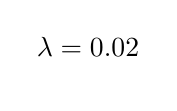
\begin{tikzpicture}[%
font=\footnotesize
]

\begin{axis}[%
width=0.951\figwidth,
height=\figheight,
at={(0\figwidth,0\figheight)},
scale only axis,
xmin=0,
xmax=3,
tick align=outside,
xlabel={Moneyness},
xmajorgrids,
ymin=0,
ymax=5,
ylabel={Remaining Time},
ymajorgrids,
zmin=0,
zmax=0.4,
zlabel={Relative Increase},
zmajorgrids,
view={50}{40},
axis background/.style={fill=white},
title style={font=\bfseries},
title={$\lambda = 0.02$},
axis x line*=bottom,
axis y line*=left,
axis z line*=left
]

\addplot3[%
surf,
shader=flat corner,draw=black,z buffer=sort,colormap={mymap}{[1pt] rgb(0pt)=(0.2081,0.1663,0.5292); rgb(1pt)=(0.211624,0.189781,0.577676); rgb(2pt)=(0.212252,0.213771,0.626971); rgb(3pt)=(0.2081,0.2386,0.677086); rgb(4pt)=(0.195905,0.264457,0.7279); rgb(5pt)=(0.170729,0.291938,0.779248); rgb(6pt)=(0.125271,0.324243,0.830271); rgb(7pt)=(0.0591333,0.359833,0.868333); rgb(8pt)=(0.0116952,0.38751,0.881957); rgb(9pt)=(0.00595714,0.408614,0.882843); rgb(10pt)=(0.0165143,0.4266,0.878633); rgb(11pt)=(0.0328524,0.443043,0.871957); rgb(12pt)=(0.0498143,0.458571,0.864057); rgb(13pt)=(0.0629333,0.47369,0.855438); rgb(14pt)=(0.0722667,0.488667,0.8467); rgb(15pt)=(0.0779429,0.503986,0.838371); rgb(16pt)=(0.0793476,0.520024,0.831181); rgb(17pt)=(0.0749429,0.537543,0.826271); rgb(18pt)=(0.0640571,0.556986,0.823957); rgb(19pt)=(0.0487714,0.577224,0.822829); rgb(20pt)=(0.0343429,0.596581,0.819852); rgb(21pt)=(0.0265,0.6137,0.8135); rgb(22pt)=(0.0238905,0.628662,0.803762); rgb(23pt)=(0.0230905,0.641786,0.791267); rgb(24pt)=(0.0227714,0.653486,0.776757); rgb(25pt)=(0.0266619,0.664195,0.760719); rgb(26pt)=(0.0383714,0.674271,0.743552); rgb(27pt)=(0.0589714,0.683757,0.725386); rgb(28pt)=(0.0843,0.692833,0.706167); rgb(29pt)=(0.113295,0.7015,0.685857); rgb(30pt)=(0.145271,0.709757,0.664629); rgb(31pt)=(0.180133,0.717657,0.642433); rgb(32pt)=(0.217829,0.725043,0.619262); rgb(33pt)=(0.258643,0.731714,0.595429); rgb(34pt)=(0.302171,0.737605,0.571186); rgb(35pt)=(0.348167,0.742433,0.547267); rgb(36pt)=(0.395257,0.7459,0.524443); rgb(37pt)=(0.44201,0.748081,0.503314); rgb(38pt)=(0.487124,0.749062,0.483976); rgb(39pt)=(0.530029,0.749114,0.466114); rgb(40pt)=(0.570857,0.748519,0.44939); rgb(41pt)=(0.609852,0.747314,0.433686); rgb(42pt)=(0.6473,0.7456,0.4188); rgb(43pt)=(0.683419,0.743476,0.404433); rgb(44pt)=(0.71841,0.741133,0.390476); rgb(45pt)=(0.752486,0.7384,0.376814); rgb(46pt)=(0.785843,0.735567,0.363271); rgb(47pt)=(0.818505,0.732733,0.34979); rgb(48pt)=(0.850657,0.7299,0.336029); rgb(49pt)=(0.882433,0.727433,0.3217); rgb(50pt)=(0.913933,0.725786,0.306276); rgb(51pt)=(0.944957,0.726114,0.288643); rgb(52pt)=(0.973895,0.731395,0.266648); rgb(53pt)=(0.993771,0.745457,0.240348); rgb(54pt)=(0.999043,0.765314,0.216414); rgb(55pt)=(0.995533,0.786057,0.196652); rgb(56pt)=(0.988,0.8066,0.179367); rgb(57pt)=(0.978857,0.827143,0.163314); rgb(58pt)=(0.9697,0.848138,0.147452); rgb(59pt)=(0.962586,0.870514,0.1309); rgb(60pt)=(0.958871,0.8949,0.113243); rgb(61pt)=(0.959824,0.921833,0.0948381); rgb(62pt)=(0.9661,0.951443,0.0755333); rgb(63pt)=(0.9763,0.9831,0.0538)},mesh/rows=25]
table[row sep=crcr, point meta=\thisrow{c}] {%
%
x	y	z	c\\
0	0.01	0.0210612144407193	0.0210612144407193\\
0	0.111836734693878	0.101411817276054	0.101411817276054\\
0	0.213673469387755	0.1649760234083	0.1649760234083\\
0	0.315510204081633	0.213143218359465	0.213143218359465\\
0	0.41734693877551	0.246941934096566	0.246941934096566\\
0	0.519183673469388	0.269691086783061	0.269691086783061\\
0	0.621020408163265	0.28472087139585	0.28472087139585\\
0	0.722857142857143	0.294597354688801	0.294597354688801\\
0	0.82469387755102	0.30109875288472	0.30109875288472\\
0	0.926530612244898	0.305401210548714	0.305401210548714\\
0	1.02836734693878	0.3082680685604	0.3082680685604\\
0	1.13020408163265	0.310192316556615	0.310192316556615\\
0	1.23204081632653	0.311493090878362	0.311493090878362\\
0	1.33387755102041	0.312378237097326	0.312378237097326\\
0	1.43571428571429	0.312984173943654	0.312984173943654\\
0	1.53755102040816	0.313401188063361	0.313401188063361\\
0	1.63938775510204	0.313689528764185	0.313689528764185\\
0	1.74122448979592	0.313889715469826	0.313889715469826\\
0	1.8430612244898	0.31402919419806	0.31402919419806\\
0	1.94489795918367	0.314126675635964	0.314126675635964\\
0	2.04673469387755	0.314194988440361	0.314194988440361\\
0	2.14857142857143	0.314242972674955	0.314242972674955\\
0	2.25040816326531	0.314276746753139	0.314276746753139\\
0	2.35224489795918	0.314300561631183	0.314300561631183\\
0	2.45408163265306	0.31431738066619	0.31431738066619\\
0	2.55591836734694	0.3143292756412	0.3143292756412\\
0	2.65775510204082	0.314337698689871	0.314337698689871\\
0	2.75959183673469	0.314343669893094	0.314343669893094\\
0	2.86142857142857	0.314347907227327	0.314347907227327\\
0	2.96326530612245	0.314350916908173	0.314350916908173\\
0	3.06510204081633	0.314353056392688	0.314353056392688\\
0	3.1669387755102	0.314354578438195	0.314354578438195\\
0	3.26877551020408	0.314355661988431	0.314355661988431\\
0	3.37061224489796	0.31435643386805	0.31435643386805\\
0	3.47244897959184	0.314356984052252	0.314356984052252\\
0	3.57428571428571	0.314357376431731	0.314357376431731\\
0	3.67612244897959	0.31435765641248	0.31435765641248\\
0	3.77795918367347	0.314357856287264	0.314357856287264\\
0	3.87979591836735	0.314357999039755	0.314357999039755\\
0	3.98163265306122	0.314358101037713	0.314358101037713\\
0	4.0834693877551	0.314358173945531	0.314358173945531\\
0	4.18530612244898	0.314358226078935	0.314358226078935\\
0	4.28714285714286	0.314358263370784	0.314358263370784\\
0	4.38897959183674	0.314358290055588	0.314358290055588\\
0	4.49081632653061	0.314358309155749	0.314358309155749\\
0	4.59265306122449	0.31435832283142	0.31435832283142\\
0	4.69448979591837	0.314358332626202	0.314358332626202\\
0	4.79632653061224	0.314358339642966	0.314358339642966\\
0	4.89816326530612	0.314358344671323	0.314358344671323\\
0	5	0.314358348275474	0.314358348275474\\
0.125	0.01	0.000100833503220867	0.000100833503220867\\
0.125	0.111836734693878	0.0279010767913849	0.0279010767913849\\
0.125	0.213673469387755	0.0620784219796874	0.0620784219796874\\
0.125	0.315510204081633	0.0916849276798692	0.0916849276798692\\
0.125	0.41734693877551	0.114453161742643	0.114453161742643\\
0.125	0.519183673469388	0.130899642969122	0.130899642969122\\
0.125	0.621020408163265	0.142402922173685	0.142402922173685\\
0.125	0.722857142857143	0.150324983985211	0.150324983985211\\
0.125	0.82469387755102	0.155746141873062	0.155746141873062\\
0.125	0.926530612244898	0.159450620079432	0.159450620079432\\
0.125	1.02836734693878	0.161985019952591	0.161985019952591\\
0.125	1.13020408163265	0.163723242272386	0.163723242272386\\
0.125	1.23204081632653	0.164919080170267	0.164919080170267\\
0.125	1.33387755102041	0.165744463503932	0.165744463503932\\
0.125	1.43571428571429	0.166315993210106	0.166315993210106\\
0.125	1.53755102040816	0.16671295989921	0.16671295989921\\
0.125	1.63938775510204	0.16698946888152	0.16698946888152\\
0.125	1.74122448979592	0.167182577998263	0.167182577998263\\
0.125	1.8430612244898	0.167317764244847	0.167317764244847\\
0.125	1.94489795918367	0.167412606344813	0.167412606344813\\
0.125	2.04673469387755	0.167479274343054	0.167479274343054\\
0.125	2.14857142857143	0.167526220341793	0.167526220341793\\
0.125	2.25040816326531	0.16755933116979	0.16755933116979\\
0.125	2.35224489795918	0.167582717664894	0.167582717664894\\
0.125	2.45408163265306	0.167599257252298	0.167599257252298\\
0.125	2.55591836734694	0.167610968312602	0.167610968312602\\
0.125	2.65775510204082	0.167619269683379	0.167619269683379\\
0.125	2.75959183673469	0.16762515910119	0.16762515910119\\
0.125	2.86142857142857	0.167629341697941	0.167629341697941\\
0.125	2.96326530612245	0.16763231441194	0.16763231441194\\
0.125	3.06510204081633	0.167634428818272	0.167634428818272\\
0.125	3.1669387755102	0.167635933784481	0.167635933784481\\
0.125	3.26877551020408	0.167637005662988	0.167637005662988\\
0.125	3.37061224489796	0.167637769542436	0.167637769542436\\
0.125	3.47244897959184	0.167638314228866	0.167638314228866\\
0.125	3.57428571428571	0.167638702821505	0.167638702821505\\
0.125	3.67612244897959	0.167638980188159	0.167638980188159\\
0.125	3.77795918367347	0.16763917825524	0.16763917825524\\
0.125	3.87979591836735	0.167639319755282	0.167639319755282\\
0.125	3.98163265306122	0.167639420884313	0.167639420884313\\
0.125	4.0834693877551	0.167639493187872	0.167639493187872\\
0.125	4.18530612244898	0.167639544900697	0.167639544900697\\
0.125	4.28714285714286	0.167639581899043	0.167639581899043\\
0.125	4.38897959183674	0.167639608378138	0.167639608378138\\
0.125	4.49081632653061	0.1676396273344	0.1676396273344\\
0.125	4.59265306122449	0.167639640908908	0.167639640908908\\
0.125	4.69448979591837	0.167639650632177	0.167639650632177\\
0.125	4.79632653061224	0.167639657598692	0.167639657598692\\
0.125	4.89816326530612	0.167639662591415	0.167639662591415\\
0.125	5	0.167639666170647	0.167639666170647\\
0.25	0.01	2.66214686692347e-09	2.66214686692347e-09\\
0.25	0.111836734693878	0.00555031627455704	0.00555031627455704\\
0.25	0.213673469387755	0.0201696360712076	0.0201696360712076\\
0.25	0.315510204081633	0.0360810394703346	0.0360810394703346\\
0.25	0.41734693877551	0.0499618751476449	0.0499618751476449\\
0.25	0.519183673469388	0.0609081528449206	0.0609081528449206\\
0.25	0.621020408163265	0.0690928119997622	0.0690928119997622\\
0.25	0.722857142857143	0.0750356938335225	0.0750356938335225\\
0.25	0.82469387755102	0.0792804984783701	0.0792804984783701\\
0.25	0.926530612244898	0.0822846941644079	0.0822846941644079\\
0.25	1.02836734693878	0.084400269295551	0.084400269295551\\
0.25	1.13020408163265	0.0858863333460597	0.0858863333460597\\
0.25	1.23204081632653	0.0869291494350704	0.0869291494350704\\
0.25	1.33387755102041	0.0876608573586514	0.0876608573586514\\
0.25	1.43571428571429	0.0881745119847969	0.0881745119847969\\
0.25	1.53755102040816	0.0885353849944235	0.0885353849944235\\
0.25	1.63938775510204	0.0887891729973598	0.0887891729973598\\
0.25	1.74122448979592	0.0889678482282147	0.0889678482282147\\
0.25	1.8430612244898	0.0890937847826229	0.0890937847826229\\
0.25	1.94489795918367	0.089182650121833	0.089182650121833\\
0.25	2.04673469387755	0.0892454263219007	0.0892454263219007\\
0.25	2.14857142857143	0.0892898200475753	0.0892898200475753\\
0.25	2.25040816326531	0.0893212461245982	0.0893212461245982\\
0.25	2.35224489795918	0.0893435139033493	0.0893435139033493\\
0.25	2.45408163265306	0.089359306637365	0.089359306637365\\
0.25	2.55591836734694	0.0893705166797123	0.0893705166797123\\
0.25	2.65775510204082	0.0893784806721059	0.0893784806721059\\
0.25	2.75959183673469	0.089384141560662	0.089384141560662\\
0.25	2.86142857142857	0.0893881691604861	0.0893881691604861\\
0.25	2.96326530612245	0.0893910363265299	0.0893910363265299\\
0.25	3.06510204081633	0.0893930786513846	0.0893930786513846\\
0.25	3.1669387755102	0.0893945342630993	0.0893945342630993\\
0.25	3.26877551020408	0.0893955722684858	0.0893955722684858\\
0.25	3.37061224489796	0.089396312849967	0.089396312849967\\
0.25	3.47244897959184	0.0893968414804761	0.0893968414804761\\
0.25	3.57428571428571	0.0893972189880907	0.0893972189880907\\
0.25	3.67612244897959	0.0893974886888739	0.0893974886888739\\
0.25	3.77795918367347	0.089397681446404	0.089397681446404\\
0.25	3.87979591836735	0.0893978192636078	0.0893978192636078\\
0.25	3.98163265306122	0.0893979178346174	0.0893979178346174\\
0.25	4.0834693877551	0.0893979883590728	0.0893979883590728\\
0.25	4.18530612244898	0.0893980388329082	0.0893980388329082\\
0.25	4.28714285714286	0.0893980749672623	0.0893980749672623\\
0.25	4.38897959183674	0.0893981008430348	0.0893981008430348\\
0.25	4.49081632653061	0.0893981193773942	0.0893981193773942\\
0.25	4.59265306122449	0.0893981326564313	0.0893981326564313\\
0.25	4.69448979591837	0.0893981421724809	0.0893981421724809\\
0.25	4.79632653061224	0.0893981489935058	0.0893981489935058\\
0.25	4.89816326530612	0.0893981538840397	0.0893981538840397\\
0.25	5	0.0893981574112996	0.0893981574112996\\
0.375	0.01	2.04267651458558e-16	2.04267651458558e-16\\
0.375	0.111836734693878	0.000747001635852109	0.000747001635852109\\
0.375	0.213673469387755	0.00550073793709336	0.00550073793709336\\
0.375	0.315510204081633	0.0127734556973785	0.0127734556973785\\
0.375	0.41734693877551	0.0202975406257651	0.0202975406257651\\
0.375	0.519183673469388	0.0269194196327807	0.0269194196327807\\
0.375	0.621020408163265	0.0322804977877542	0.0322804977877542\\
0.375	0.722857142857143	0.0364188103247275	0.0364188103247275\\
0.375	0.82469387755102	0.0395222413968566	0.0395222413968566\\
0.375	0.926530612244898	0.0418073968681112	0.0418073968681112\\
0.375	1.02836734693878	0.0434700407258645	0.0434700407258645\\
0.375	1.13020408163265	0.0446701423944658	0.0446701423944658\\
0.375	1.23204081632653	0.0455317238664222	0.0455317238664222\\
0.375	1.33387755102041	0.0461480221716413	0.0461480221716413\\
0.375	1.43571428571429	0.0465877913125947	0.0465877913125947\\
0.375	1.53755102040816	0.0469010952422038	0.0469010952422038\\
0.375	1.63938775510204	0.0471240808240492	0.0471240808240492\\
0.375	1.74122448979592	0.047282696487885	0.047282696487885\\
0.375	1.8430612244898	0.0473954965292703	0.0473954965292703\\
0.375	1.94489795918367	0.0474757129822674	0.0474757129822674\\
0.375	2.04673469387755	0.047532765867478	0.047532765867478\\
0.375	2.14857142857143	0.0475733540804885	0.0475733540804885\\
0.375	2.25040816326531	0.0476022384761313	0.0476022384761313\\
0.375	2.35224489795918	0.0476228016070153	0.0476228016070153\\
0.375	2.45408163265306	0.047637446663443	0.047637446663443\\
0.375	2.55591836734694	0.0476478812736578	0.0476478812736578\\
0.375	2.65775510204082	0.0476553191175082	0.0476553191175082\\
0.375	2.75959183673469	0.0476606231173549	0.0476606231173549\\
0.375	2.86142857142857	0.0476644070460476	0.0476644070460476\\
0.375	2.96326530612245	0.04766710765252	0.04766710765252\\
0.375	3.06510204081633	0.0476690358588647	0.0476690358588647\\
0.375	3.1669387755102	0.0476704131122646	0.0476704131122646\\
0.375	3.26877551020408	0.0476713972056028	0.0476713972056028\\
0.375	3.37061224489796	0.0476721006254625	0.0476721006254625\\
0.375	3.47244897959184	0.047672603673461	0.047672603673461\\
0.375	3.57428571428571	0.0476729634616934	0.0476729634616934\\
0.375	3.67612244897959	0.0476732207660967	0.0476732207660967\\
0.375	3.77795918367347	0.0476734049978726	0.0476734049978726\\
0.375	3.87979591836735	0.0476735368939722	0.0476735368939722\\
0.375	3.98163265306122	0.0476736313479866	0.0476736313479866\\
0.375	4.0834693877551	0.0476736990068831	0.0476736990068831\\
0.375	4.18530612244898	0.0476737474844302	0.0476737474844302\\
0.375	4.28714285714286	0.0476737822270898	0.0476737822270898\\
0.375	4.38897959183674	0.0476738071321667	0.0476738071321667\\
0.375	4.49081632653061	0.0476738249892716	0.0476738249892716\\
0.375	4.59265306122449	0.0476738377957201	0.0476738377957201\\
0.375	4.69448979591837	0.047673846981948	0.047673846981948\\
0.375	4.79632653061224	0.0476738535726727	0.0476738535726727\\
0.375	4.89816326530612	0.0476738583021515	0.0476738583021515\\
0.375	5	0.047673861696641	0.047673861696641\\
0.5	0.01	3.70536611252091e-26	3.70536611252091e-26\\
0.5	0.111836734693878	6.47637307356003e-05	6.47637307356003e-05\\
0.5	0.213673469387755	0.00122868780757813	0.00122868780757813\\
0.5	0.315510204081633	0.00400600789210862	0.00400600789210862\\
0.5	0.41734693877551	0.00758934264157903	0.00758934264157903\\
0.5	0.519183673469388	0.0112017180242988	0.0112017180242988\\
0.5	0.621020408163265	0.0144173107949824	0.0144173107949824\\
0.5	0.722857142857143	0.0170827611178683	0.0170827611178683\\
0.5	0.82469387755102	0.0191965595771385	0.0191965595771385\\
0.5	0.926530612244898	0.0208248464773075	0.0208248464773075\\
0.5	1.02836734693878	0.0220543875619789	0.0220543875619789\\
0.5	1.13020408163265	0.0229698265468261	0.0229698265468261\\
0.5	1.23204081632653	0.0236444745533528	0.0236444745533528\\
0.5	1.33387755102041	0.0241379380847513	0.0241379380847513\\
0.5	1.43571428571429	0.0244968573802957	0.0244968573802957\\
0.5	1.53755102040816	0.0247568205055746	0.0247568205055746\\
0.5	1.63938775510204	0.0249445156394064	0.0249445156394064\\
0.5	1.74122448979592	0.0250797110836103	0.0250797110836103\\
0.5	1.8430612244898	0.0251769183322897	0.0251769183322897\\
0.5	1.94489795918367	0.0252467193475162	0.0252467193475162\\
0.5	2.04673469387755	0.0252967924336458	0.0252967924336458\\
0.5	2.14857142857143	0.0253326883093435	0.0253326883093435\\
0.5	2.25040816326531	0.0253584084588792	0.0253584084588792\\
0.5	2.35224489795918	0.0253768315113591	0.0253768315113591\\
0.5	2.45408163265306	0.0253900251077226	0.0253900251077226\\
0.5	2.55591836734694	0.0253994726783522	0.0253994726783522\\
0.5	2.65775510204082	0.0254062376280172	0.0254062376280172\\
0.5	2.75959183673469	0.0254110818161099	0.0254110818161099\\
0.5	2.86142857142857	0.025414550846139	0.025414550846139\\
0.5	2.96326530612245	0.0254170353505539	0.0254170353505539\\
0.5	3.06510204081633	0.0254188149676405	0.0254188149676405\\
0.5	3.1669387755102	0.0254200898675057	0.0254200898675057\\
0.5	3.26877551020408	0.0254210033363881	0.0254210033363881\\
0.5	3.37061224489796	0.0254216579475122	0.0254216579475122\\
0.5	3.47244897959184	0.0254221271360422	0.0254221271360422\\
0.5	3.57428571428571	0.0254224634827298	0.0254224634827298\\
0.5	3.67612244897959	0.0254227046415723	0.0254227046415723\\
0.5	3.77795918367347	0.0254228775814788	0.0254228775814788\\
0.5	3.87979591836735	0.025423001621611	0.025423001621611\\
0.5	3.98163265306122	0.0254230906036572	0.0254230906036572\\
0.5	4.0834693877551	0.0254231544466251	0.0254231544466251\\
0.5	4.18530612244898	0.0254232002572038	0.0254232002572038\\
0.5	4.28714285714286	0.025423233139827	0.025423233139827\\
0.5	4.38897959183674	0.0254232567443759	0.0254232567443759\\
0.5	4.49081632653061	0.0254232736913822	0.0254232736913822\\
0.5	4.59265306122449	0.0254232858604327	0.0254232858604327\\
0.5	4.69448979591837	0.0254232945999046	0.0254232945999046\\
0.5	4.79632653061224	0.0254233008772622	0.0254233008772622\\
0.5	4.89816326530612	0.0254233053867798	0.0254233053867798\\
0.5	5	0.0254233086267668	0.0254233086267668\\
0.625	0.01	1.46096456877253e-38	1.46096456877253e-38\\
0.625	0.111836734693878	3.49673882180298e-06	3.49673882180298e-06\\
0.625	0.213673469387755	0.000220315384340969	0.000220315384340969\\
0.625	0.315510204081633	0.00109812750793995	0.00109812750793995\\
0.625	0.41734693877551	0.00258561704562312	0.00258561704562312\\
0.625	0.519183673469388	0.00435326486394044	0.00435326486394044\\
0.625	0.621020408163265	0.00611354244831109	0.00611354244831109\\
0.625	0.722857142857143	0.00769842025311003	0.00769842025311003\\
0.625	0.82469387755102	0.00903842144898309	0.00903842144898309\\
0.625	0.926530612244898	0.0101249945189476	0.0101249945189476\\
0.625	1.02836734693878	0.0109807622847261	0.0109807622847261\\
0.625	1.13020408163265	0.0116407098410204	0.0116407098410204\\
0.625	1.23204081632653	0.0121417555273557	0.0121417555273557\\
0.625	1.33387755102041	0.01251768495424	0.01251768495424\\
0.625	1.43571428571429	0.0127971861731337	0.0127971861731337\\
0.625	1.53755102040816	0.0130035280959781	0.0130035280959781\\
0.625	1.63938775510204	0.0131550166845087	0.0131550166845087\\
0.625	1.74122448979592	0.0132657474851469	0.0132657474851469\\
0.625	1.8430612244898	0.0133464053084128	0.0133464053084128\\
0.625	1.94489795918367	0.0134049951216451	0.0134049951216451\\
0.625	2.04673469387755	0.0134474608177275	0.0134474608177275\\
0.625	2.14857142857143	0.0134781855211974	0.0134781855211974\\
0.625	2.25040816326531	0.0135003840519806	0.0135003840519806\\
0.625	2.35224489795918	0.0135164043641174	0.0135164043641174\\
0.625	2.45408163265306	0.0135279555582124	0.0135279555582124\\
0.625	2.55591836734694	0.013536278401666	0.013536278401666\\
0.625	2.65775510204082	0.0135422717564862	0.0135422717564862\\
0.625	2.75959183673469	0.0135465856947449	0.0135465856947449\\
0.625	2.86142857142857	0.0135496897251706	0.0135496897251706\\
0.625	2.96326530612245	0.0135519225808757	0.0135519225808757\\
0.625	3.06510204081633	0.0135535284352097	0.0135535284352097\\
0.625	3.1669387755102	0.0135546831784598	0.0135546831784598\\
0.625	3.26877551020408	0.0135555134445744	0.0135555134445744\\
0.625	3.37061224489796	0.0135561103660239	0.0135561103660239\\
0.625	3.47244897959184	0.0135565395047005	0.0135565395047005\\
0.625	3.57428571428571	0.0135568480145727	0.0135568480145727\\
0.625	3.67612244897959	0.0135570698035079	0.0135570698035079\\
0.625	3.77795918367347	0.0135572292507505	0.0135572292507505\\
0.625	3.87979591836735	0.0135573438828194	0.0135573438828194\\
0.625	3.98163265306122	0.0135574262988747	0.0135574262988747\\
0.625	4.0834693877551	0.0135574855556223	0.0135574855556223\\
0.625	4.18530612244898	0.0135575281632236	0.0135575281632236\\
0.625	4.28714285714286	0.0135575588013399	0.0135575588013399\\
0.625	4.38897959183674	0.0135575808338874	0.0135575808338874\\
0.625	4.49081632653061	0.0135575966790519	0.0135575966790519\\
0.625	4.59265306122449	0.0135576080752454	0.0135576080752454\\
0.625	4.69448979591837	0.0135576162722608	0.0135576162722608\\
0.625	4.79632653061224	0.0135576221686611	0.0135576221686611\\
0.625	4.89816326530612	0.0135576264105259	0.0135576264105259\\
0.625	5	0.0135576294629702	0.0135576294629702\\
0.75	0.01	1.20144152682882e-53	1.20144152682882e-53\\
0.75	0.111836734693878	1.14922562443957e-07	1.14922562443957e-07\\
0.75	0.213673469387755	3.12176441978003e-05	3.12176441978003e-05\\
0.75	0.315510204081633	0.000260135717045182	0.000260135717045182\\
0.75	0.41734693877551	0.000795624864217264	0.000795624864217264\\
0.75	0.519183673469388	0.00156859203088547	0.00156859203088547\\
0.75	0.621020408163265	0.00244597749370263	0.00244597749370263\\
0.75	0.722857142857143	0.00331481976719069	0.00331481976719069\\
0.75	0.82469387755102	0.00410503006068181	0.00410503006068181\\
0.75	0.926530612244898	0.00478409245853629	0.00478409245853629\\
0.75	1.02836734693878	0.00534489221959566	0.00534489221959566\\
0.75	1.13020408163265	0.00579480963401666	0.00579480963401666\\
0.75	1.23204081632653	0.00614802108320021	0.00614802108320021\\
0.75	1.33387755102041	0.00642074033659151	0.00642074033659151\\
0.75	1.43571428571429	0.00662859850920996	0.00662859850920996\\
0.75	1.53755102040816	0.00678540697457767	0.00678540697457767\\
0.75	1.63938775510204	0.00690273941711247	0.00690273941711247\\
0.75	1.74122448979592	0.00698995681623389	0.00698995681623389\\
0.75	1.8430612244898	0.00705444262084189	0.00705444262084189\\
0.75	1.94489795918367	0.00710191353604491	0.00710191353604491\\
0.75	2.04673469387755	0.00713673394299865	0.00713673394299865\\
0.75	2.14857142857143	0.00716219968760527	0.00716219968760527\\
0.75	2.25040816326531	0.00718077844039767	0.00718077844039767\\
0.75	2.35224489795918	0.00719430522236949	0.00719430522236949\\
0.75	2.45408163265306	0.00720413712315528	0.00720413712315528\\
0.75	2.55591836734694	0.00721127331580948	0.00721127331580948\\
0.75	2.65775510204082	0.00721644678134127	0.00721644678134127\\
0.75	2.75959183673469	0.00722019362132778	0.00722019362132778\\
0.75	2.86142857142857	0.00722290497421356	0.00722290497421356\\
0.75	2.96326530612245	0.00722486563098718	0.00722486563098718\\
0.75	3.06510204081633	0.00722628259787296	0.00722628259787296\\
0.75	3.1669387755102	0.00722730612816153	0.00722730612816153\\
0.75	3.26877551020408	0.00722804515206609	0.00722804515206609\\
0.75	3.37061224489796	0.0072285785627576	0.0072285785627576\\
0.75	3.47244897959184	0.00722896345101801	0.00722896345101801\\
0.75	3.57428571428571	0.00722924110119671	0.00722924110119671\\
0.75	3.67612244897959	0.00722944134964796	0.00722944134964796\\
0.75	3.77795918367347	0.00722958574835332	0.00722958574835332\\
0.75	3.87979591836735	0.0072296898585364	0.0072296898585364\\
0.75	3.98163265306122	0.00722976491185999	0.00722976491185999\\
0.75	4.0834693877551	0.00722981901256755	0.00722981901256755\\
0.75	4.18530612244898	0.00722985800680577	0.00722985800680577\\
0.75	4.28714285714286	0.00722988611089296	0.00722988611089296\\
0.75	4.38897959183674	0.00722990636514444	0.00722990636514444\\
0.75	4.49081632653061	0.00722992096154922	0.00722992096154922\\
0.75	4.59265306122449	0.00722993148027683	0.00722993148027683\\
0.75	4.69448979591837	0.00722993906032846	0.00722993906032846\\
0.75	4.79632653061224	0.00722994452263773	0.00722994452263773\\
0.75	4.89816326530612	0.00722994845885111	0.00722994845885111\\
0.75	5	0.00722995129534492	0.00722995129534492\\
0.875	0.01	2.01370079391801e-71	2.01370079391801e-71\\
0.875	0.111836734693878	2.26376363123292e-09	2.26376363123292e-09\\
0.875	0.213673469387755	3.45364429572326e-06	3.45364429572326e-06\\
0.875	0.315510204081633	5.27581902666862e-05	5.27581902666862e-05\\
0.875	0.41734693877551	0.000219465695387696	0.000219465695387696\\
0.875	0.519183673469388	0.000520727470470505	0.000520727470470505\\
0.875	0.621020408163265	0.00091820683667713	0.00091820683667713\\
0.875	0.722857142857143	0.00135691207315857	0.00135691207315857\\
0.875	0.82469387755102	0.00179022791205935	0.00179022791205935\\
0.875	0.926530612244898	0.00218769441191863	0.00218769441191863\\
0.875	1.02836734693878	0.00253383066724731	0.00253383066724731\\
0.875	1.13020408163265	0.00282405560454595	0.00282405560454595\\
0.875	1.23204081632653	0.00306055955555124	0.00306055955555124\\
0.875	1.33387755102041	0.00324909859148047	0.00324909859148047\\
0.875	1.43571428571429	0.00339683097181878	0.00339683097181878\\
0.875	1.53755102040816	0.00351100951572318	0.00351100951572318\\
0.875	1.63938775510204	0.00359828318619031	0.00359828318619031\\
0.875	1.74122448979592	0.00366439283634219	0.00366439283634219\\
0.875	1.8430612244898	0.00371410123095741	0.00371410123095741\\
0.875	1.94489795918367	0.00375124911213506	0.00375124911213506\\
0.875	2.04673469387755	0.00377886913421397	0.00377886913421397\\
0.875	2.14857142857143	0.00379931760460282	0.00379931760460282\\
0.875	2.25040816326531	0.00381440238501378	0.00381440238501378\\
0.875	2.35224489795918	0.00382549669473893	0.00382549669473893\\
0.875	2.45408163265306	0.00383363519398829	0.00383363519398829\\
0.875	2.55591836734694	0.00383959232026659	0.00383959232026659\\
0.875	2.65775510204082	0.00384394459106793	0.00384394459106793\\
0.875	2.75959183673469	0.00384711925240956	0.00384711925240956\\
0.875	2.86142857142857	0.0038494317360831	0.0038494317360831\\
0.875	2.96326530612245	0.00385111418534077	0.00385111418534077\\
0.875	3.06510204081633	0.00385233698984543	0.00385233698984543\\
0.875	3.1669387755102	0.00385322492891503	0.00385322492891503\\
0.875	3.26877551020408	0.00385386920354699	0.00385386920354699\\
0.875	3.37061224489796	0.00385433636179045	0.00385433636179045\\
0.875	3.47244897959184	0.00385467489354401	0.00385467489354401\\
0.875	3.57428571428571	0.00385492008727499	0.00385492008727499\\
0.875	3.67612244897959	0.00385509759680393	0.00385509759680393\\
0.875	3.77795918367347	0.0038552260545954	0.0038552260545954\\
0.875	3.87979591836735	0.00385531898261321	0.00385531898261321\\
0.875	3.98163265306122	0.00385538618715604	0.00385538618715604\\
0.875	4.0834693877551	0.00385543477552497	0.00385543477552497\\
0.875	4.18530612244898	0.00385546989611202	0.00385546989611202\\
0.875	4.28714285714286	0.00385549527656076	0.00385549527656076\\
0.875	4.38897959183674	0.00385551361472121	0.00385551361472121\\
0.875	4.49081632653061	0.00385552686242996	0.00385552686242996\\
0.875	4.59265306122449	0.00385553643134697	0.00385553643134697\\
0.875	4.69448979591837	0.00385554334216309	0.00385554334216309\\
0.875	4.79632653061224	0.00385554833269802	0.00385554833269802\\
0.875	4.89816326530612	0.00385555193617718	0.00385555193617718\\
0.875	5	0.0038555545378901	0.0038555545378901\\
1	0.01	6.78220443089767e-92	6.78220443089767e-92\\
1	0.111836734693878	2.64414769201089e-11	2.64414769201089e-11\\
1	0.213673469387755	2.95604849806789e-07	2.95604849806789e-07\\
1	0.315510204081633	9.09136102723464e-06	9.09136102723464e-06\\
1	0.41734693877551	5.3923784280748e-05	5.3923784280748e-05\\
1	0.519183673469388	0.000158392224192938	0.000158392224192938\\
1	0.621020408163265	0.000321832646909248	0.000321832646909248\\
1	0.722857142857143	0.000525690758395303	0.000525690758395303\\
1	0.82469387755102	0.000746555998450207	0.000746555998450207\\
1	0.926530612244898	0.000964437871571848	0.000964437871571848\\
1	1.02836734693878	0.0011657054291813	0.0011657054291813\\
1	1.13020408163265	0.00134291661961338	0.00134291661961338\\
1	1.23204081632653	0.00149340859021096	0.00149340859021096\\
1	1.33387755102041	0.00161769303585979	0.00161769303585979\\
1	1.43571428571429	0.00171810310227695	0.00171810310227695\\
1	1.53755102040816	0.00179781128971776	0.00179781128971776\\
1	1.63938775510204	0.00186019060025239	0.00186019060025239\\
1	1.74122448979592	0.00190844181139716	0.00190844181139716\\
1	1.8430612244898	0.00194540621564984	0.00194540621564984\\
1	1.94489795918367	0.0019734971035374	0.0019734971035374\\
1	2.04673469387755	0.00199470098759361	0.00199470098759361\\
1	2.14857142857143	0.00201061537946912	0.00201061537946912\\
1	2.25040816326531	0.00202250213240902	0.00202250213240902\\
1	2.35224489795918	0.0020313439888751	0.0020313439888751\\
1	2.45408163265306	0.00203789769359043	0.00203789769359043\\
1	2.55591836734694	0.00204274061472019	0.00204274061472019\\
1	2.65775510204082	0.00204630992788792	0.00204630992788792\\
1	2.75959183673469	0.00204893457049331	0.00204893457049331\\
1	2.86142857142857	0.00205086073053708	0.00205086073053708\\
1	2.96326530612245	0.0020522718393968	0.0020522718393968\\
1	3.06510204081633	0.00205330404921575	0.00205330404921575\\
1	3.1669387755102	0.00205405809000666	0.00205405809000666\\
1	3.26877551020408	0.00205460827658814	0.00205460827658814\\
1	3.37061224489796	0.00205500930298777	0.00205500930298777\\
1	3.47244897959184	0.00205530133826586	0.00205530133826586\\
1	3.57428571428571	0.00205551382992421	0.00205551382992421\\
1	3.67612244897959	0.00205566833108809	0.00205566833108809\\
1	3.77795918367347	0.00205578059472563	0.00205578059472563\\
1	3.87979591836735	0.00205586212031194	0.00205586212031194\\
1	3.98163265306122	0.00205592129317538	0.00205592129317538\\
1	4.0834693877551	0.00205596422193377	0.00205596422193377\\
1	4.18530612244898	0.00205599535283656	0.00205599535283656\\
1	4.28714285714286	0.00205601791968804	0.00205601791968804\\
1	4.38897959183674	0.00205603427287054	0.00205603427287054\\
1	4.49081632653061	0.00205604611964369	0.00205604611964369\\
1	4.59265306122449	0.0020560546994445	0.0020560546994445\\
1	4.69448979591837	0.00205606091164111	0.00205606091164111\\
1	4.79632653061224	0.0020560654085527	0.0020560654085527\\
1	4.89816326530612	0.00205606866312515	0.00205606866312515\\
1	5	0.00205607101813273	0.00205607101813273\\
1.125	0.01	4.54779037811358e-115	4.54779037811358e-115\\
1.125	0.111836734693878	1.81747757747062e-13	1.81747757747062e-13\\
1.125	0.213673469387755	1.94399541240484e-08	1.94399541240484e-08\\
1.125	0.315510204081633	1.32303862909959e-06	1.32303862909959e-06\\
1.125	0.41734693877551	1.1739436801095e-05	1.1739436801095e-05\\
1.125	0.519183673469388	4.39383810311113e-05	4.39383810311113e-05\\
1.125	0.621020408163265	0.000104875664045125	0.000104875664045125\\
1.125	0.722857142857143	0.000191991810425363	0.000191991810425363\\
1.125	0.82469387755102	0.000296595757718867	0.000296595757718867\\
1.125	0.926530612244898	0.000408444210611959	0.000408444210611959\\
1.125	1.02836734693878	0.000518709656001117	0.000518709656001117\\
1.125	1.13020408163265	0.000621161728221224	0.000621161728221224\\
1.125	1.23204081632653	0.000712200044727672	0.000712200044727672\\
1.125	1.33387755102041	0.000790354958242666	0.000790354958242666\\
1.125	1.43571428571429	0.000855650323184364	0.000855650323184364\\
1.125	1.53755102040816	0.000909025871543095	0.000909025871543095\\
1.125	1.63938775510204	0.000951891335975131	0.000951891335975131\\
1.125	1.74122448979592	0.000985818334728446	0.000985818334728446\\
1.125	1.8430612244898	0.00101234786350509	0.00101234786350509\\
1.125	1.94489795918367	0.00103288378943279	0.00103288378943279\\
1.125	2.04673469387755	0.00104864494344477	0.00104864494344477\\
1.125	2.14857142857143	0.00106065405475979	0.00106065405475979\\
1.125	2.25040816326531	0.00106974780052789	0.00106974780052789\\
1.125	2.35224489795918	0.00107659738846555	0.00107659738846555\\
1.125	2.45408163265306	0.0010817330091774	0.0010817330091774\\
1.125	2.55591836734694	0.00108556826397623	0.00108556826397623\\
1.125	2.65775510204082	0.00108842251725504	0.00108842251725504\\
1.125	2.75959183673469	0.00109054028257168	0.00109054028257168\\
1.125	2.86142857142857	0.0010921074377593	0.0010921074377593\\
1.125	2.96326530612245	0.00109326443792673	0.00109326443792673\\
1.125	3.06510204081633	0.00109411687225859	0.00109411687225859\\
1.125	3.1669387755102	0.00109474377042294	0.00109474377042294\\
1.125	3.26877551020408	0.00109520405908203	0.00109520405908203\\
1.125	3.37061224489796	0.00109554153107852	0.00109554153107852\\
1.125	3.47244897959184	0.00109578863888141	0.00109578863888141\\
1.125	3.57428571428571	0.00109596937087526	0.00109596937087526\\
1.125	3.67612244897959	0.00109610141979782	0.00109610141979782\\
1.125	3.77795918367347	0.00109619780960243	0.00109619780960243\\
1.125	3.87979591836735	0.00109626811093943	0.00109626811093943\\
1.125	3.98163265306122	0.00109631934603278	0.00109631934603278\\
1.125	4.0834693877551	0.00109635666023489	0.00109635666023489\\
1.125	4.18530612244898	0.00109638381907461	0.00109638381907461\\
1.125	4.28714285714286	0.00109640357527429	0.00109640357527429\\
1.125	4.38897959183674	0.00109641793918902	0.00109641793918902\\
1.125	4.49081632653061	0.00109642837771566	0.00109642837771566\\
1.125	4.59265306122449	0.00109643596035304	0.00109643596035304\\
1.125	4.69448979591837	0.00109644146629971	0.00109644146629971\\
1.125	4.79632653061224	0.00109644546288144	0.00109644546288144\\
1.125	4.89816326530612	0.00109644836291706	0.00109644836291706\\
1.125	5	0.00109645046663554	0.00109645046663554\\
1.25	0.01	6.03256166089891e-141	6.03256166089891e-141\\
1.25	0.111836734693878	7.31108614199509e-16	7.31108614199509e-16\\
1.25	0.213673469387755	9.77091736852902e-10	9.77091736852902e-10\\
1.25	0.315510204081633	1.61810044676926e-07	1.61810044676926e-07\\
1.25	0.41734693877551	2.25454579052367e-06	2.25454579052367e-06\\
1.25	0.519183673469388	1.1071683272054e-05	1.1071683272054e-05\\
1.25	0.621020408163265	3.16580269037885e-05	3.16580269037885e-05\\
1.25	0.722857142857143	6.58742099399352e-05	6.58742099399352e-05\\
1.25	0.82469387755102	0.000111890237522309	0.000111890237522309\\
1.25	0.926530612244898	0.00016565063701591	0.00016565063701591\\
1.25	1.02836734693878	0.000222569486790926	0.000222569486790926\\
1.25	1.13020408163265	0.000278660632255577	0.000278660632255577\\
1.25	1.23204081632653	0.000331030852370428	0.000331030852370428\\
1.25	1.33387755102041	0.000377929713859463	0.000377929713859463\\
1.25	1.43571428571429	0.000418569552781124	0.000418569552781124\\
1.25	1.53755102040816	0.000452867957539803	0.000452867957539803\\
1.25	1.63938775510204	0.00048119877856356	0.00048119877856356\\
1.25	1.74122448979592	0.000504189398953562	0.000504189398953562\\
1.25	1.8430612244898	0.000522573274040831	0.000522573274040831\\
1.25	1.94489795918367	0.000537092505549975	0.000537092505549975\\
1.25	2.04673469387755	0.000548439910580791	0.000548439910580791\\
1.25	2.14857142857143	0.00055722950230435	0.00055722950230435\\
1.25	2.25040816326531	0.000563985869582381	0.000563985869582381\\
1.25	2.35224489795918	0.000569145145564596	0.000569145145564596\\
1.25	2.45408163265306	0.000573062367281516	0.000573062367281516\\
1.25	2.55591836734694	0.000576021764708528	0.000576021764708528\\
1.25	2.65775510204082	0.000578247821903557	0.000578247821903557\\
1.25	2.75959183673469	0.000579915870050303	0.000579915870050303\\
1.25	2.86142857142857	0.000581161582265553	0.000581161582265553\\
1.25	2.96326530612245	0.000582089123783831	0.000582089123783831\\
1.25	3.06510204081633	0.000582777937318501	0.000582777937318501\\
1.25	3.1669387755102	0.000583288265031608	0.000583288265031608\\
1.25	3.26877551020408	0.000583665564035163	0.000583665564035163\\
1.25	3.37061224489796	0.000583943988206412	0.000583943988206412\\
1.25	3.47244897959184	0.000584149102873631	0.000584149102873631\\
1.25	3.57428571428571	0.000584299981755969	0.000584299981755969\\
1.25	3.67612244897959	0.000584410814171775	0.000584410814171775\\
1.25	3.77795918367347	0.000584492128819987	0.000584492128819987\\
1.25	3.87979591836735	0.000584551720401175	0.000584551720401175\\
1.25	3.98163265306122	0.000584595347864961	0.000584595347864961\\
1.25	4.0834693877551	0.000584627258380556	0.000584627258380556\\
1.25	4.18530612244898	0.000584650579104401	0.000584650579104401\\
1.25	4.28714285714286	0.000584667609171871	0.000584667609171871\\
1.25	4.38897959183674	0.000584680036716598	0.000584680036716598\\
1.25	4.49081632653061	0.000584689099769414	0.000584689099769414\\
1.25	4.59265306122449	0.000584695705288116	0.000584695705288116\\
1.25	4.69448979591837	0.000584700517041433	0.000584700517041433\\
1.25	4.79632653061224	0.000584704020383706	0.000584704020383706\\
1.25	4.89816326530612	0.000584706569922196	0.000584706569922196\\
1.25	5	0.000584708424545832	0.000584708424545832\\
1.375	0.01	1.57570726682024e-169	1.57570726682024e-169\\
1.375	0.111836734693878	1.71410607083159e-18	1.71410607083159e-18\\
1.375	0.213673469387755	3.73822912855091e-11	3.73822912855091e-11\\
1.375	0.315510204081633	1.65666691589853e-08	1.65666691589853e-08\\
1.375	0.41734693877551	3.80574291200537e-07	3.80574291200537e-07\\
1.375	0.519183673469388	2.52571064762282e-06	2.52571064762282e-06\\
1.375	0.621020408163265	8.82458001051231e-06	8.82458001051231e-06\\
1.375	0.722857142857143	2.1170670120425e-05	2.1170670120425e-05\\
1.375	0.82469387755102	3.99667046699234e-05	3.99667046699234e-05\\
1.375	0.926530612244898	6.41569839667547e-05	6.41569839667547e-05\\
1.375	1.02836734693878	9.18396115223287e-05	9.18396115223287e-05\\
1.375	1.13020408163265	0.000120923035021832	0.000120923035021832\\
1.375	1.23204081632653	0.000149575773245354	0.000149575773245354\\
1.375	1.33387755102041	0.000176437578315181	0.000176437578315181\\
1.375	1.43571428571429	0.000200653770753743	0.000200653770753743\\
1.375	1.53755102040816	0.000221809580728335	0.000221809580728335\\
1.375	1.63938775510204	0.000239824576037987	0.000239824576037987\\
1.375	1.74122448979592	0.000254844406685706	0.000254844406685706\\
1.375	1.8430612244898	0.00026714841043006	0.00026714841043006\\
1.375	1.94489795918367	0.000277079349863661	0.000277079349863661\\
1.375	2.04673469387755	0.000284994749269684	0.000284994749269684\\
1.375	2.14857142857143	0.000291236250705933	0.000291236250705933\\
1.375	2.25040816326531	0.000296112580652729	0.000296112580652729\\
1.375	2.35224489795918	0.000299892021051854	0.000299892021051854\\
1.375	2.45408163265306	0.000302801036437571	0.000302801036437571\\
1.375	2.55591836734694	0.000305026551665876	0.000305026551665876\\
1.375	2.65775510204082	0.000306720127627538	0.000306720127627538\\
1.375	2.75959183673469	0.000308002883281762	0.000308002883281762\\
1.375	2.86142857142857	0.000308970457536219	0.000308970457536219\\
1.375	2.96326530612245	0.000309697615510003	0.000309697615510003\\
1.375	3.06510204081633	0.000310242309682517	0.000310242309682517\\
1.375	3.1669387755102	0.000310649135343812	0.000310649135343812\\
1.375	3.26877551020408	0.000310952194989908	0.000310952194989908\\
1.375	3.37061224489796	0.000311177425830997	0.000311177425830997\\
1.375	3.47244897959184	0.000311344461468701	0.000311344461468701\\
1.375	3.57428571428571	0.000311468102124956	0.000311468102124956\\
1.375	3.67612244897959	0.000311559463617999	0.000311559463617999\\
1.375	3.77795918367347	0.000311626867448299	0.000311626867448299\\
1.375	3.87979591836735	0.000311676525238711	0.000311676525238711\\
1.375	3.98163265306122	0.000311713061721315	0.000311713061721315\\
1.375	4.0834693877551	0.000311739912183569	0.000311739912183569\\
1.375	4.18530612244898	0.000311759623083314	0.000311759623083314\\
1.375	4.28714285714286	0.000311774078485896	0.000311774078485896\\
1.375	4.38897959183674	0.000311784670008613	0.000311784670008613\\
1.375	4.49081632653061	0.000311792423958059	0.000311792423958059\\
1.375	4.59265306122449	0.000311798096172627	0.000311798096172627\\
1.375	4.69448979591837	0.000311802242594377	0.000311802242594377\\
1.375	4.79632653061224	0.00031180527166224	0.00031180527166224\\
1.375	4.89816326530612	0.000311807483130103	0.000311807483130103\\
1.375	5	0.000311809096774438	0.000311809096774438\\
1.5	0.01	8.07676323186891e-201	8.07676323186891e-201\\
1.5	0.111836734693878	2.33494476136992e-21	2.33494476136992e-21\\
1.5	0.213673469387755	1.08520422113478e-12	1.08520422113478e-12\\
1.5	0.315510204081633	1.41547711468213e-09	1.41547711468213e-09\\
1.5	0.41734693877551	5.62972739269069e-08	5.62972739269069e-08\\
1.5	0.519183673469388	5.20144780397308e-07	5.20144780397308e-07\\
1.5	0.621020408163265	2.26537380618273e-06	2.26537380618273e-06\\
1.5	0.722857142857143	6.35657586300626e-06	6.35657586300626e-06\\
1.5	0.82469387755102	1.34833836287231e-05	1.34833836287231e-05\\
1.5	0.926530612244898	2.36712617705661e-05	2.36712617705661e-05\\
1.5	1.02836734693878	3.63553176187686e-05	3.63553176187686e-05\\
1.5	1.13020408163265	5.0637057580026e-05	5.0637057580026e-05\\
1.5	1.23204081632653	6.5548173381794e-05	6.5548173381794e-05\\
1.5	1.33387755102041	8.02354729617851e-05	8.02354729617851e-05\\
1.5	1.43571428571429	9.40529985091303e-05	9.40529985091303e-05\\
1.5	1.53755102040816	0.000106581791161048	0.000106581791161048\\
1.5	1.63938775510204	0.000117605829557312	0.000117605829557312\\
1.5	1.74122448979592	0.000127068230545504	0.000127068230545504\\
1.5	1.8430612244898	0.000135023817163042	0.000135023817163042\\
1.5	1.94489795918367	0.00014159688578147	0.00014159688578147\\
1.5	2.04673469387755	0.000146947801700685	0.000146947801700685\\
1.5	2.14857142857143	0.000151248901263406	0.000151248901263406\\
1.5	2.25040816326531	0.000154668578685173	0.000154668578685173\\
1.5	2.35224489795918	0.000157361838350169	0.000157361838350169\\
1.5	2.45408163265306	0.000159465560932019	0.000159465560932019\\
1.5	2.55591836734694	0.000161096967491486	0.000161096967491486\\
1.5	2.65775510204082	0.000162354090979959	0.000162354090979959\\
1.5	2.75959183673469	0.000163317384279892	0.000163317384279892\\
1.5	2.86142857142857	0.000164051865778973	0.000164051865778973\\
1.5	2.96326530612245	0.000164609415340472	0.000164609415340472\\
1.5	3.06510204081633	0.000165030988450059	0.000165030988450059\\
1.5	3.1669387755102	0.000165348623652224	0.000165348623652224\\
1.5	3.26877551020408	0.00016558718895872	0.00016558718895872\\
1.5	3.37061224489796	0.000165765856659883	0.000165765856659883\\
1.5	3.47244897959184	0.000165899321066437	0.000165899321066437\\
1.5	3.57428571428571	0.000165998786410533	0.000165998786410533\\
1.5	3.67612244897959	0.000166072756989428	0.000166072756989428\\
1.5	3.77795918367347	0.000166127661812146	0.000166127661812146\\
1.5	3.87979591836735	0.000166168343629462	0.000166168343629462\\
1.5	3.98163265306122	0.000166198438652028	0.000166198438652028\\
1.5	4.0834693877551	0.000166220669322988	0.000166220669322988\\
1.5	4.18530612244898	0.000166237068686546	0.000166237068686546\\
1.5	4.28714285714286	0.000166249151428796	0.000166249151428796\\
1.5	4.38897959183674	0.000166258043664115	0.000166258043664115\\
1.5	4.49081632653061	0.000166264581017151	0.000166264581017151\\
1.5	4.59265306122449	0.000166269382478286	0.000166269382478286\\
1.5	4.69448979591837	0.000166272905838369	0.000166272905838369\\
1.5	4.79632653061224	0.000166275489177953	0.000166275489177953\\
1.5	4.89816326530612	0.000166277381839438	0.000166277381839438\\
1.5	5	0.0001662787674946	0.0001662787674946\\
1.625	0.01	8.10317636009083e-235	8.10317636009083e-235\\
1.625	0.111836734693878	1.84349925172316e-24	1.84349925172316e-24\\
1.625	0.213673469387755	2.38444616277535e-14	2.38444616277535e-14\\
1.625	0.315510204081633	1.00672696575467e-10	1.00672696575467e-10\\
1.625	0.41734693877551	7.27993682570679e-09	7.27993682570679e-09\\
1.625	0.519183673469388	9.64716888451344e-08	9.64716888451344e-08\\
1.625	0.621020408163265	5.3435056096308e-07	5.3435056096308e-07\\
1.625	0.722857142857143	1.77917492883616e-06	1.77917492883616e-06\\
1.625	0.82469387755102	4.28699042716966e-06	4.28699042716966e-06\\
1.625	0.926530612244898	8.30224743742751e-06	8.30224743742751e-06\\
1.625	1.02836734693878	1.37769917260645e-05	1.37769917260645e-05\\
1.625	1.13020408163265	2.04188470244636e-05	2.04188470244636e-05\\
1.625	1.23204081632653	2.78001636817835e-05	2.78001636817835e-05\\
1.625	1.33387755102041	3.546713379388e-05	3.546713379388e-05\\
1.625	1.43571428571429	4.30177935300801e-05	4.30177935300801e-05\\
1.625	1.53755102040816	5.01428117127417e-05	5.01428117127417e-05\\
1.625	1.63938775510204	5.66360569067032e-05	5.66360569067032e-05\\
1.625	1.74122448979592	6.23858042134958e-05	6.23858042134958e-05\\
1.625	1.8430612244898	6.73563819070052e-05	6.73563819070052e-05\\
1.625	1.94489795918367	7.15672426816048e-05	7.15672426816048e-05\\
1.625	2.04673469387755	7.50735960065945e-05	7.50735960065945e-05\\
1.625	2.14857142857143	7.79505397999087e-05	7.79505397999087e-05\\
1.625	2.25040816326531	8.02811949702981e-05	8.02811949702981e-05\\
1.625	2.35224489795918	8.21485462446898e-05	8.21485462446898e-05\\
1.625	2.45408163265306	8.36303360159706e-05	8.36303360159706e-05\\
1.625	2.55591836734694	8.4796272743694e-05	8.4796272743694e-05\\
1.625	2.65775510204082	8.57068743961112e-05	8.57068743961112e-05\\
1.625	2.75959183673469	8.64133875023512e-05	8.64133875023512e-05\\
1.625	2.86142857142857	8.69583552107334e-05	8.69583552107334e-05\\
1.625	2.96326530612245	8.73765287076187e-05	8.73765287076187e-05\\
1.625	3.06510204081633	8.76959155434625e-05	8.76959155434625e-05\\
1.625	3.1669387755102	8.79388341759548e-05	8.79388341759548e-05\\
1.625	3.26877551020408	8.81228987396919e-05	8.81228987396919e-05\\
1.625	3.37061224489796	8.8261895579653e-05	8.8261895579653e-05\\
1.625	3.47244897959184	8.83665375086008e-05	8.83665375086008e-05\\
1.625	3.57428571428571	8.84450966716296e-05	8.84450966716296e-05\\
1.625	3.67612244897959	8.8503925243015e-05	8.8503925243015e-05\\
1.625	3.77795918367347	8.85478771635434e-05	8.85478771635434e-05\\
1.625	3.87979591836735	8.85806453645245e-05	8.85806453645245e-05\\
1.625	3.98163265306122	8.8605028542736e-05	8.8605028542736e-05\\
1.625	4.0834693877551	8.86231403026518e-05	8.86231403026518e-05\\
1.625	4.18530612244898	8.86365718528838e-05	8.86365718528838e-05\\
1.625	4.28714285714286	8.86465177286101e-05	8.86465177286101e-05\\
1.625	4.38897959183674	8.86538723790955e-05	8.86538723790955e-05\\
1.625	4.49081632653061	8.86593039944317e-05	8.86593039944317e-05\\
1.625	4.59265306122449	8.86633106815816e-05	8.86633106815816e-05\\
1.625	4.69448979591837	8.86662630392914e-05	8.86662630392914e-05\\
1.625	4.79632653061224	8.86684363101829e-05	8.86684363101829e-05\\
1.625	4.89816326530612	8.86700345843053e-05	8.86700345843053e-05\\
1.625	5	8.86712089669632e-05	8.86712089669632e-05\\
1.75	0.01	1.58798613668989e-271	1.58798613668989e-271\\
1.75	0.111836734693878	8.41981610760086e-28	8.41981610760086e-28\\
1.75	0.213673469387755	3.95756883366851e-16	3.95756883366851e-16\\
1.75	0.315510204081633	5.9479964988131e-12	5.9479964988131e-12\\
1.75	0.41734693877551	8.21238242387191e-10	8.21238242387191e-10\\
1.75	0.519183673469388	1.608190137649e-08	1.608190137649e-08\\
1.75	0.621020408163265	1.1558556656004e-07	1.1558556656004e-07\\
1.75	0.722857142857143	4.63331222662686e-07	4.63331222662686e-07\\
1.75	0.82469387755102	1.28216250548632e-06	1.28216250548632e-06\\
1.75	0.926530612244898	2.76284175491524e-06	2.76284175491524e-06\\
1.75	1.02836734693878	4.98859123717116e-06	4.98859123717116e-06\\
1.75	1.13020408163265	7.91373518086514e-06	7.91373518086514e-06\\
1.75	1.23204081632653	1.13894015045339e-05	1.13894015045339e-05\\
1.75	1.33387755102041	1.52106246550211e-05	1.52106246550211e-05\\
1.75	1.43571428571429	1.91625488251354e-05	1.91625488251354e-05\\
1.75	1.53755102040816	2.30540053464517e-05	2.30540053464517e-05\\
1.75	1.63938775510204	2.6735800942548e-05	2.6735800942548e-05\\
1.75	1.74122448979592	3.01061633943834e-05	3.01061633943834e-05\\
1.75	1.8430612244898	3.31075669094361e-05	3.31075669094361e-05\\
1.75	1.94489795918367	3.57189767421737e-05	3.57189767421737e-05\\
1.75	2.04673469387755	3.79465551390248e-05	3.79465551390248e-05\\
1.75	2.14857142857143	3.98147488267856e-05	3.98147488267856e-05\\
1.75	2.25040816326531	4.13587498070856e-05	4.13587498070856e-05\\
1.75	2.35224489795918	4.26186746201315e-05	4.26186746201315e-05\\
1.75	2.45408163265306	4.36354182728766e-05	4.36354182728766e-05\\
1.75	2.55591836734694	4.44479436463723e-05	4.44479436463723e-05\\
1.75	2.65775510204082	4.5091699026144e-05	4.5091699026144e-05\\
1.75	2.75959183673469	4.55978618399591e-05	4.55978618399591e-05\\
1.75	2.86142857142857	4.5993148132254e-05	4.5993148132254e-05\\
1.75	2.96326530612245	4.62999811246247e-05	4.62999811246247e-05\\
1.75	3.06510204081633	4.65368651687141e-05	4.65368651687141e-05\\
1.75	3.1669387755102	4.67188571807576e-05	4.67188571807576e-05\\
1.75	3.26877551020408	4.68580641449532e-05	4.68580641449532e-05\\
1.75	3.37061224489796	4.69641226631275e-05	4.69641226631275e-05\\
1.75	3.47244897959184	4.70446360518432e-05	4.70446360518432e-05\\
1.75	3.57428571428571	4.71055577287799e-05	4.71055577287799e-05\\
1.75	3.67612244897959	4.71515181308915e-05	4.71515181308915e-05\\
1.75	3.77795918367347	4.71860974962084e-05	4.71860974962084e-05\\
1.75	3.87979591836735	4.72120495803753e-05	4.72120495803753e-05\\
1.75	3.98163265306122	4.72314825709679e-05	4.72314825709679e-05\\
1.75	4.0834693877551	4.72460036887852e-05	4.72460036887852e-05\\
1.75	4.18530612244898	4.72568336305195e-05	4.72568336305195e-05\\
1.75	4.28714285714286	4.72648963825842e-05	4.72648963825842e-05\\
1.75	4.38897959183674	4.72708891952052e-05	4.72708891952052e-05\\
1.75	4.49081632653061	4.72753367547248e-05	4.72753367547248e-05\\
1.75	4.59265306122449	4.72786328897266e-05	4.72786328897266e-05\\
1.75	4.69448979591837	4.72810725221778e-05	4.72810725221778e-05\\
1.75	4.79632653061224	4.72828760385059e-05	4.72828760385059e-05\\
1.75	4.89816326530612	4.7284207806473e-05	4.7284207806473e-05\\
1.75	5	4.72851901948994e-05	4.72851901948994e-05\\
1.875	0.01	6.06890238857451e-311	6.06890238857451e-311\\
1.875	0.111836734693878	2.22119151389802e-31	2.22119151389802e-31\\
1.875	0.213673469387755	4.95376304615393e-18	4.95376304615393e-18\\
1.875	0.315510204081633	2.91440973052905e-13	2.91440973052905e-13\\
1.875	0.41734693877551	8.06809108863629e-11	8.06809108863629e-11\\
1.875	0.519183673469388	2.4054668209667e-09	2.4054668209667e-09\\
1.875	0.621020408163265	2.28899963800849e-08	2.28899963800849e-08\\
1.875	0.722857142857143	1.1207975911983e-07	1.1207975911983e-07\\
1.875	0.82469387755102	3.60133007757791e-07	3.60133007757791e-07\\
1.875	0.926530612244898	8.70955897666704e-07	8.70955897666704e-07\\
1.875	1.02836734693878	1.72317035249474e-06	1.72317035249474e-06\\
1.875	1.13020408163265	2.94307364810682e-06	2.94307364810682e-06\\
1.875	1.23204081632653	4.49980126307137e-06	4.49980126307137e-06\\
1.875	1.33387755102041	6.31818435562366e-06	6.31818435562366e-06\\
1.875	1.43571428571429	8.29936603230447e-06	8.29936603230447e-06\\
1.875	1.53755102040816	1.03407438197344e-05	1.03407438197344e-05\\
1.875	1.63938775510204	1.23506686581412e-05	1.23506686581412e-05\\
1.875	1.74122448979592	1.42567343964025e-05	1.42567343964025e-05\\
1.875	1.8430612244898	1.6008528674338e-05	1.6008528674338e-05\\
1.875	1.94489795918367	1.75765158190906e-05	1.75765158190906e-05\\
1.875	2.04673469387755	1.89487366033735e-05	1.89487366033735e-05\\
1.875	2.14857142857143	2.01266565189151e-05	2.01266565189151e-05\\
1.875	2.25040816326531	2.11210500538535e-05	2.11210500538535e-05\\
1.875	2.35224489795918	2.19484158720326e-05	2.19484158720326e-05\\
1.875	2.45408163265306	2.26281280478225e-05	2.26281280478225e-05\\
1.875	2.55591836734694	2.31803427553223e-05	2.31803427553223e-05\\
1.875	2.65775510204082	2.36245777989858e-05	2.36245777989858e-05\\
1.875	2.75959183673469	2.39788389769629e-05	2.39788389769629e-05\\
1.875	2.86142857142857	2.42591602669295e-05	2.42591602669295e-05\\
1.875	2.96326530612245	2.44794375006076e-05	2.44794375006076e-05\\
1.875	3.06510204081633	2.46514563244608e-05	2.46514563244608e-05\\
1.875	3.1669387755102	2.47850380452684e-05	2.47850380452684e-05\\
1.875	3.26877551020408	2.48882478163053e-05	2.48882478163053e-05\\
1.875	3.37061224489796	2.49676269774543e-05	2.49676269774543e-05\\
1.875	3.47244897959184	2.50284248824643e-05	2.50284248824643e-05\\
1.875	3.57428571428571	2.50748155296621e-05	2.50748155296621e-05\\
1.875	3.67612244897959	2.51100913337063e-05	2.51100913337063e-05\\
1.875	3.77795918367347	2.51368310728671e-05	2.51368310728671e-05\\
1.875	3.87979591836735	2.51570420089676e-05	2.51570420089676e-05\\
1.875	3.98163265306122	2.51722779016868e-05	2.51722779016868e-05\\
1.875	4.0834693877551	2.51837355167337e-05	2.51837355167337e-05\\
1.875	4.18530612244898	2.51923325525419e-05	2.51923325525419e-05\\
1.875	4.28714285714286	2.51987698947403e-05	2.51987698947403e-05\\
1.875	4.38897959183674	2.52035808990164e-05	2.52035808990164e-05\\
1.875	4.49081632653061	2.52071700994144e-05	2.52071700994144e-05\\
1.875	4.59265306122449	2.52098434033223e-05	2.52098434033223e-05\\
1.875	4.69448979591837	2.52118315041328e-05	2.52118315041328e-05\\
1.875	4.79632653061224	2.52133079386125e-05	2.52133079386125e-05\\
1.875	4.89816326530612	2.52144029481138e-05	2.52144029481138e-05\\
1.875	5	2.52152140737607e-05	2.52152140737607e-05\\
2	0.01	0	0\\
2	0.111836734693878	3.3802452449005e-35	3.3802452449005e-35\\
2	0.213673469387755	4.6702131383527e-20	4.6702131383527e-20\\
2	0.315510204081633	1.18263296325349e-14	1.18263296325349e-14\\
2	0.41734693877551	6.89307510885987e-12	6.89307510885987e-12\\
2	0.519183673469388	3.22374986901762e-10	3.22374986901762e-10\\
2	0.621020408163265	4.14410666097302e-09	4.14410666097302e-09\\
2	0.722857142857143	2.51482987732146e-08	2.51482987732146e-08\\
2	0.82469387755102	9.48632376959877e-08	9.48632376959877e-08\\
2	0.926530612244898	2.59717184600699e-07	2.59717184600699e-07\\
2	1.02836734693878	5.67001250974461e-07	5.67001250974461e-07\\
2	1.13020408163265	1.04871906357673e-06	1.04871906357673e-06\\
2	1.23204081632653	1.71191287026904e-06	1.71191287026904e-06\\
2	1.33387755102041	2.53808447135521e-06	2.53808447135521e-06\\
2	1.43571428571429	3.48944020785625e-06	3.48944020785625e-06\\
2	1.53755102040816	4.51802969905659e-06	4.51802969905659e-06\\
2	1.63938775510204	5.57449260392657e-06	5.57449260392657e-06\\
2	1.74122448979592	6.61458547409615e-06	6.61458547409615e-06\\
2	1.8430612244898	7.60297538814836e-06	7.60297538814836e-06\\
2	1.94489795918367	8.51461396805722e-06	8.51461396805722e-06\\
2	2.04673469387755	9.33436290049223e-06	9.33436290049223e-06\\
2	2.14857142857143	1.00555812861328e-05	1.00555812861328e-05\\
2	2.25040816326531	1.06782609435057e-05	1.06782609435057e-05\\
2	2.35224489795918	1.12071191606099e-05	1.12071191606099e-05\\
2	2.45408163265306	1.16498920461178e-05	1.16498920461178e-05\\
2	2.55591836734694	1.20159421949023e-05	1.20159421949023e-05\\
2	2.65775510204082	1.23152066910475e-05	1.23152066910475e-05\\
2	2.75959183673469	1.25574597675869e-05	1.25574597675869e-05\\
2	2.86142857142857	1.27518394328756e-05	1.27518394328756e-05\\
2	2.96326530612245	1.29065799714702e-05	1.29065799714702e-05\\
2	3.06510204081633	1.30288951100844e-05	1.30288951100844e-05\\
2	3.1669387755102	1.31249645826525e-05	1.31249645826525e-05\\
2	3.26877551020408	1.31999864653857e-05	1.31999864653857e-05\\
2	3.37061224489796	1.32582670352197e-05	1.32582670352197e-05\\
2	3.47244897959184	1.33033280663454e-05	1.33033280663454e-05\\
2	3.57428571428571	1.33380180727443e-05	1.33380180727443e-05\\
2	3.67612244897959	1.33646190381313e-05	1.33646190381313e-05\\
2	3.77795918367347	1.33849438338571e-05	1.33849438338571e-05\\
2	3.87979591836735	1.34004220618503e-05	1.34004220618503e-05\\
2	3.98163265306122	1.34121737287802e-05	1.34121737287802e-05\\
2	4.0834693877551	1.34210711865473e-05	1.34210711865473e-05\\
2	4.18530612244898	1.34277903501952e-05	1.34277903501952e-05\\
2	4.28714285714286	1.34328524733725e-05	1.34328524733725e-05\\
2	4.38897959183674	1.34366578324712e-05	1.34366578324712e-05\\
2	4.49081632653061	1.34395126217106e-05	1.34395126217106e-05\\
2	4.59265306122449	1.34416502467511e-05	1.34416502467511e-05\\
2	4.69448979591837	1.3443248059805e-05	1.3443248059805e-05\\
2	4.79632653061224	1.34444404273437e-05	1.34444404273437e-05\\
2	4.89816326530612	1.34453288758891e-05	1.34453288758891e-05\\
2	5	1.34459899292113e-05	1.34459899292113e-05\\
2.125	0.01	0	0\\
2.125	0.111836734693878	2.96442250859177e-39	2.96442250859177e-39\\
2.125	0.213673469387755	3.31254231920638e-22	3.31254231920638e-22\\
2.125	0.315510204081633	3.96980286028441e-16	3.96980286028441e-16\\
2.125	0.41734693877551	5.11535101202155e-13	5.11535101202155e-13\\
2.125	0.519183673469388	3.86627491545828e-11	3.86627491545828e-11\\
2.125	0.621020408163265	6.85055472178312e-10	6.85055472178312e-10\\
2.125	0.722857142857143	5.2276012824678e-09	5.2276012824678e-09\\
2.125	0.82469387755102	2.34053052703968e-08	2.34053052703968e-08\\
2.125	0.926530612244898	7.31699330612116e-08	7.31699330612116e-08\\
2.125	1.02836734693878	1.77501374948982e-07	1.77501374948982e-07\\
2.125	1.13020408163265	3.57603553811625e-07	3.57603553811625e-07\\
2.125	1.23204081632653	6.26324203692588e-07	6.26324203692588e-07\\
2.125	1.33387755102041	9.8470763563071e-07	9.8470763563071e-07\\
2.125	1.43571428571429	1.42229696706136e-06	1.42229696706136e-06\\
2.125	1.53755102040816	1.92012662336743e-06	1.92012662336743e-06\\
2.125	1.63938775510204	2.45481939901779e-06	2.45481939901779e-06\\
2.125	1.74122448979592	3.00247557473929e-06	3.00247557473929e-06\\
2.125	1.8430612244898	3.54160677236692e-06	3.54160677236692e-06\\
2.125	1.94489795918367	4.05488703059807e-06	4.05488703059807e-06\\
2.125	2.04673469387755	4.5298347204654e-06	4.5298347204654e-06\\
2.125	2.14857142857143	4.95869849447731e-06	4.95869849447731e-06\\
2.125	2.25040816326531	5.3378496964179e-06	5.3378496964179e-06\\
2.125	2.35224489795918	5.66694066498905e-06	5.66694066498905e-06\\
2.125	2.45408163265306	5.94801787600914e-06	5.94801787600914e-06\\
2.125	2.55591836734694	6.18470821418541e-06	6.18470821418541e-06\\
2.125	2.65775510204082	6.38153892047453e-06	6.38153892047453e-06\\
2.125	2.75959183673469	6.54341067622311e-06	6.54341067622311e-06\\
2.125	2.86142857142857	6.67521758739302e-06	6.67521758739302e-06\\
2.125	2.96326530612245	6.78159418890278e-06	6.78159418890278e-06\\
2.125	3.06510204081633	6.86676433498651e-06	6.86676433498651e-06\\
2.125	3.1669387755102	6.93446680751011e-06	6.93446680751011e-06\\
2.125	3.26877551020408	6.98793526589599e-06	6.98793526589599e-06\\
2.125	3.37061224489796	7.02991414630599e-06	7.02991414630599e-06\\
2.125	3.47244897959184	7.06269628451727e-06	7.06269628451727e-06\\
2.125	3.57428571428571	7.08817183417711e-06	7.08817183417711e-06\\
2.125	3.67612244897959	7.10788123388323e-06	7.10788123388323e-06\\
2.125	3.77795918367347	7.12306748484287e-06	7.12306748484287e-06\\
2.125	3.87979591836735	7.13472488122016e-06	7.13472488122016e-06\\
2.125	3.98163265306122	7.14364268089297e-06	7.14364268089297e-06\\
2.125	4.0834693877551	7.15044312214529e-06	7.15044312214529e-06\\
2.125	4.18530612244898	7.15561378372291e-06	7.15561378372291e-06\\
2.125	4.28714285714286	7.15953463969823e-06	7.15953463969823e-06\\
2.125	4.38897959183674	7.16250034798763e-06	7.16250034798763e-06\\
2.125	4.49081632653061	7.16473838710472e-06	7.16473838710472e-06\\
2.125	4.59265306122449	7.16642366051527e-06	7.16642366051527e-06\\
2.125	4.69448979591837	7.16769015082104e-06	7.16769015082104e-06\\
2.125	4.79632653061224	7.16864014688922e-06	7.16864014688922e-06\\
2.125	4.89816326530612	7.16935149911022e-06	7.16935149911022e-06\\
2.125	5	7.16988328943825e-06	7.16988328943825e-06\\
2.25	0.01	0	0\\
2.25	0.111836734693878	1.49688139516549e-43	1.49688139516549e-43\\
2.25	0.213673469387755	1.76610431589983e-24	1.76610431589983e-24\\
2.25	0.315510204081633	1.10125737050404e-17	1.10125737050404e-17\\
2.25	0.41734693877551	3.293962039819e-14	3.293962039819e-14\\
2.25	0.519183673469388	4.14515822549872e-12	4.14515822549872e-12\\
2.25	0.621020408163265	1.03293069343573e-10	1.03293069343573e-10\\
2.25	0.722857142857143	1.00564928999563e-09	1.00564928999563e-09\\
2.25	0.82469387755102	5.40315141754094e-09	5.40315141754094e-09\\
2.25	0.926530612244898	1.94546254437482e-08	1.94546254437482e-08\\
2.25	1.02836734693878	5.2808653731319e-08	5.2808653731319e-08\\
2.25	1.13020408163265	1.16558203469966e-07	1.16558203469966e-07\\
2.25	1.23204081632653	2.20113624232671e-07	2.20113624232671e-07\\
2.25	1.33387755102041	3.68538005436476e-07	3.68538005436476e-07\\
2.25	1.43571428571429	5.61331217925316e-07	5.61331217925316e-07\\
2.25	1.53755102040816	7.92774405842251e-07	7.92774405842251e-07\\
2.25	1.63938775510204	1.05335555081538e-06	1.05335555081538e-06\\
2.25	1.74122448979592	1.33162488538573e-06	1.33162488538573e-06\\
2.25	1.8430612244898	1.61594471464069e-06	1.61594471464069e-06\\
2.25	1.94489795918367	1.89582237287301e-06	1.89582237287301e-06\\
2.25	2.04673469387755	2.16272473376767e-06	2.16272473376767e-06\\
2.25	2.14857142857143	2.41041545661734e-06	2.41041545661734e-06\\
2.25	2.25040816326531	2.63492748126979e-06	2.63492748126979e-06\\
2.25	2.35224489795918	2.8343007000883e-06	2.8343007000883e-06\\
2.25	2.45408163265306	3.00820027921964e-06	3.00820027921964e-06\\
2.25	2.55591836734694	3.15750290421976e-06	3.15750290421976e-06\\
2.25	2.65775510204082	3.2839081357026e-06	3.2839081357026e-06\\
2.25	2.75959183673469	3.38960630528241e-06	3.38960630528241e-06\\
2.25	2.86142857142857	3.47701522888772e-06	3.47701522888772e-06\\
2.25	2.96326530612245	3.54858541233461e-06	3.54858541233461e-06\\
2.25	3.06510204081633	3.60666623118995e-06	3.60666623118995e-06\\
2.25	3.1669387755102	3.65342232699175e-06	3.65342232699175e-06\\
2.25	3.26877551020408	3.69078881807807e-06	3.69078881807807e-06\\
2.25	3.37061224489796	3.72045479139298e-06	3.72045479139298e-06\\
2.25	3.47244897959184	3.74386614283752e-06	3.74386614283752e-06\\
2.25	3.57428571428571	3.76224065881714e-06	3.76224065881714e-06\\
2.25	3.67612244897959	3.77658998071177e-06	3.77658998071177e-06\\
2.25	3.77795918367347	3.7877446151372e-06	3.7877446151372e-06\\
2.25	3.87979591836735	3.7963793903407e-06	3.7963793903407e-06\\
2.25	3.98163265306122	3.80303771415054e-06	3.80303771415054e-06\\
2.25	4.0834693877551	3.80815369256058e-06	3.80815369256058e-06\\
2.25	4.18530612244898	3.81207166333337e-06	3.81207166333337e-06\\
2.25	4.28714285714286	3.8150630305931e-06	3.8150630305931e-06\\
2.25	4.38897959183674	3.81734049490991e-06	3.81734049490991e-06\\
2.25	4.49081632653061	3.81906989310292e-06	3.81906989310292e-06\\
2.25	4.59265306122449	3.82037992022175e-06	3.82037992022175e-06\\
2.25	4.69448979591837	3.82137002375157e-06	3.82137002375157e-06\\
2.25	4.79632653061224	3.82211675233752e-06	3.82211675233752e-06\\
2.25	4.89816326530612	3.8226788190908e-06	3.8226788190908e-06\\
2.25	5	3.82310111021724e-06	3.82310111021724e-06\\
2.375	0.01	0	0\\
2.375	0.111836734693878	4.34885579548061e-48	4.34885579548061e-48\\
2.375	0.213673469387755	7.07246341378294e-27	7.07246341378294e-27\\
2.375	0.315510204081633	2.52264645155028e-19	2.52264645155028e-19\\
2.375	0.41734693877551	1.83894706767872e-15	1.83894706767872e-15\\
2.375	0.519183673469388	3.96934748091982e-13	3.96934748091982e-13\\
2.375	0.621020408163265	1.41929008773711e-11	1.41929008773711e-11\\
2.375	0.722857142857143	1.78870795661806e-10	1.78870795661806e-10\\
2.375	0.82469387755102	1.16597879349309e-09	1.16597879349309e-09\\
2.375	0.926530612244898	4.87708649058411e-09	4.87708649058411e-09\\
2.375	1.02836734693878	1.4916818368587e-08	1.4916818368587e-08\\
2.375	1.13020408163265	3.62789507869968e-08	3.62789507869968e-08\\
2.375	1.23204081632653	7.42309940147864e-08	7.42309940147864e-08\\
2.375	1.33387755102041	1.32915997672856e-07	1.32915997672856e-07\\
2.375	1.43571428571429	2.14275828563904e-07	2.14275828563904e-07\\
2.375	1.53755102040816	3.17631067697776e-07	3.17631067697776e-07\\
2.375	1.63938775510204	4.39917091418435e-07	4.39917091418435e-07\\
2.375	1.74122448979592	5.76361918163501e-07	5.76361918163501e-07\\
2.375	1.8430612244898	7.2133409831974e-07	7.2133409831974e-07\\
2.375	1.94489795918367	8.6913821506889e-07	8.6913821506889e-07\\
2.375	2.04673469387755	1.01462623153874e-06	1.01462623153874e-06\\
2.375	2.14857142857143	1.15357899827693e-06	1.15357899827693e-06\\
2.375	2.25040816326531	1.2828727553342e-06	1.2828727553342e-06\\
2.375	2.35224489795918	1.40047744811736e-06	1.40047744811736e-06\\
2.375	2.45408163265306	1.50534314205961e-06	1.50534314205961e-06\\
2.375	2.55591836734694	1.59722621230901e-06	1.59722621230901e-06\\
2.375	2.65775510204082	1.67649569227244e-06	1.67649569227244e-06\\
2.375	2.75959183673469	1.74394731717897e-06	1.74394731717897e-06\\
2.375	2.86142857142857	1.80064130575524e-06	1.80064130575524e-06\\
2.375	2.96326530612245	1.84777102273368e-06	1.84777102273368e-06\\
2.375	3.06510204081633	1.88656354278777e-06	1.88656354278777e-06\\
2.375	3.1669387755102	1.91820942994415e-06	1.91820942994415e-06\\
2.375	3.26877551020408	1.94381718715151e-06	1.94381718715151e-06\\
2.375	3.37061224489796	1.96438724354809e-06	1.96438724354809e-06\\
2.375	3.47244897959184	1.98080054610847e-06	1.98080054610847e-06\\
2.375	3.57428571428571	1.99381744129866e-06	1.99381744129866e-06\\
2.375	3.67612244897959	2.00408331934269e-06	2.00408331934269e-06\\
2.375	3.77795918367347	2.01213829129836e-06	2.01213829129836e-06\\
2.375	3.87979591836735	2.01842889013047e-06	2.01842889013047e-06\\
2.375	3.98163265306122	2.02332039213899e-06	2.02332039213899e-06\\
2.375	4.0834693877551	2.02710883543661e-06	2.02710883543661e-06\\
2.375	4.18530612244898	2.03003217580452e-06	2.03003217580452e-06\\
2.375	4.28714285714286	2.032280283575e-06	2.032280283575e-06\\
2.375	4.38897959183674	2.03400366722651e-06	2.03400366722651e-06\\
2.375	4.49081632653061	2.03532092857076e-06	2.03532092857076e-06\\
2.375	4.59265306122449	2.03632502698259e-06	2.03632502698259e-06\\
2.375	4.69448979591837	2.03708846945244e-06	2.03708846945244e-06\\
2.375	4.79632653061224	2.03766755985363e-06	2.03766755985363e-06\\
2.375	4.89816326530612	2.03810584266237e-06	2.03810584266237e-06\\
2.375	5	2.03843686924061e-06	2.03843686924061e-06\\
2.5	0.01	0	0\\
2.5	0.111836734693878	7.26499514186167e-53	7.26499514186167e-53\\
2.5	0.213673469387755	2.12590501853039e-29	2.12590501853039e-29\\
2.5	0.315510204081633	4.76838618718414e-21	4.76838618718414e-21\\
2.5	0.41734693877551	8.89423566634638e-17	8.89423566634638e-17\\
2.5	0.519183673469388	3.39229588452774e-14	3.39229588452774e-14\\
2.5	0.621020408163265	1.7757540034621e-12	1.7757540034621e-12\\
2.5	0.722857142857143	2.93921573634834e-11	2.93921573634834e-11\\
2.5	0.82469387755102	2.35011875631807e-10	2.35011875631807e-10\\
2.5	0.926530612244898	1.15182043148116e-09	1.15182043148116e-09\\
2.5	1.02836734693878	3.99712268314398e-09	3.99712268314398e-09\\
2.5	1.13020408163265	1.07736028295151e-08	1.07736028295151e-08\\
2.5	1.23204081632653	2.40008500667052e-08	2.40008500667052e-08\\
2.5	1.33387755102041	4.61520916935665e-08	4.61520916935665e-08\\
2.5	1.43571428571429	7.90381092761863e-08	7.90381092761863e-08\\
2.5	1.53755102040816	1.23372497808017e-07	1.23372497808017e-07\\
2.5	1.63938775510204	1.78632074682673e-07	1.78632074682673e-07\\
2.5	1.74122448979592	2.43196093740356e-07	2.43196093740356e-07\\
2.5	1.8430612244898	3.14668674646213e-07	3.14668674646213e-07\\
2.5	1.94489795918367	3.90269447866399e-07	3.90269447866399e-07\\
2.5	2.04673469387755	4.67198538501597e-07	4.67198538501597e-07\\
2.5	2.14857142857143	5.4291931478868e-07	5.4291931478868e-07\\
2.5	2.25040816326531	6.15338209008376e-07	6.15338209008376e-07\\
2.5	2.35224489795918	6.82886874152728e-07	6.82886874152728e-07\\
2.5	2.45408163265306	7.44526339518106e-07	7.44526339518106e-07\\
2.5	2.55591836734694	7.99697735421743e-07	7.99697735421743e-07\\
2.5	2.65775510204082	8.48242834886699e-07	8.48242834886699e-07\\
2.5	2.75959183673469	8.90313139511327e-07	8.90313139511327e-07\\
2.5	2.86142857142857	9.2628073752518e-07	9.2628073752518e-07\\
2.5	2.96326530612245	9.56659028447086e-07	9.56659028447086e-07\\
2.5	3.06510204081633	9.82037280943679e-07	9.82037280943679e-07\\
2.5	3.1669387755102	1.00303003626704e-06	1.00303003626704e-06\\
2.5	3.26877551020408	1.02024048992455e-06	1.02024048992455e-06\\
2.5	3.37061224489796	1.03423596223274e-06	1.03423596223274e-06\\
2.5	3.47244897959184	1.04553316302957e-06	1.04553316302957e-06\\
2.5	3.57428571428571	1.05459095118535e-06	1.05459095118535e-06\\
2.5	3.67612244897959	1.06180851506684e-06	1.06180851506684e-06\\
2.5	3.77795918367347	1.06752723315012e-06	1.06752723315012e-06\\
2.5	3.87979591836735	1.07203483390111e-06	1.07203483390111e-06\\
2.5	3.98163265306122	1.07557081299266e-06	1.07557081299266e-06\\
2.5	4.0834693877551	1.07833235955691e-06	1.07833235955691e-06\\
2.5	4.18530612244898	1.08048028269171e-06	1.08048028269171e-06\\
2.5	4.28714285714286	1.08214461549444e-06	1.08214461549444e-06\\
2.5	4.38897959183674	1.08342971217819e-06	1.08342971217819e-06\\
2.5	4.49081632653061	1.08441875217545e-06	1.08441875217545e-06\\
2.5	4.59265306122449	1.08517763174968e-06	1.08517763174968e-06\\
2.5	4.69448979591837	1.08575826608143e-06	1.08575826608143e-06\\
2.5	4.79632653061224	1.08620134954404e-06	1.08620134954404e-06\\
2.5	4.89816326530612	1.08653863417896e-06	1.08653863417896e-06\\
2.5	5	1.08679479029499e-06	1.08679479029499e-06\\
2.625	0.01	0	0\\
2.625	0.111836734693878	6.97491895354044e-58	6.97491895354044e-58\\
2.625	0.213673469387755	4.79397520444576e-32	4.79397520444576e-32\\
2.625	0.315510204081633	7.43322145812735e-23	7.43322145812735e-23\\
2.625	0.41734693877551	3.72445842159809e-18	3.72445842159809e-18\\
2.625	0.519183673469388	2.58569561309784e-15	2.58569561309784e-15\\
2.625	0.621020408163265	2.02166051294827e-13	2.02166051294827e-13\\
2.625	0.722857142857143	4.45879222188519e-12	4.45879222188519e-12\\
2.625	0.82469387755102	4.42112877155501e-11	4.42112877155501e-11\\
2.625	0.926530612244898	2.56081691386326e-10	2.56081691386326e-10\\
2.625	1.02836734693878	1.01530122881005e-09	1.01530122881005e-09\\
2.625	1.13020408163265	3.05020699759037e-09	3.05020699759037e-09\\
2.625	1.23204081632653	7.43410305266879e-09	7.43410305266879e-09\\
2.625	1.33387755102041	1.54159478199472e-08	1.54159478199472e-08\\
2.625	1.43571428571429	2.81475791181378e-08	2.81475791181378e-08\\
2.625	1.53755102040816	4.64143706032152e-08	4.64143706032152e-08\\
2.625	1.63938775510204	7.04598481100777e-08	7.04598481100777e-08\\
2.625	1.74122448979592	9.99426647978111e-08	9.99426647978111e-08\\
2.625	1.8430612244898	1.34013226444207e-07	1.34013226444207e-07\\
2.625	1.94489795918367	1.71467310788056e-07	1.71467310788056e-07\\
2.625	2.04673469387755	2.10927383349192e-07	2.10927383349192e-07\\
2.625	2.14857142857143	2.51011432271877e-07	2.51011432271877e-07\\
2.625	2.25040816326531	2.90464724672357e-07	2.90464724672357e-07\\
2.625	2.35224489795918	3.28245049796473e-07	3.28245049796473e-07\\
2.625	2.45408163265306	3.63563263968259e-07	3.63563263968259e-07\\
2.625	2.55591836734694	3.95887464028357e-07	3.95887464028357e-07\\
2.625	2.65775510204082	4.24921591126366e-07	4.24921591126366e-07\\
2.625	2.75959183673469	4.50568976272409e-07	4.50568976272409e-07\\
2.625	2.86142857142857	4.7288953330106e-07	4.7288953330106e-07\\
2.625	2.96326530612245	4.92056945875753e-07	4.92056945875753e-07\\
2.625	3.06510204081633	5.08319899290465e-07	5.08319899290465e-07\\
2.625	3.1669387755102	5.21969495507359e-07	5.21969495507359e-07\\
2.625	3.26877551020408	5.33313571157881e-07	5.33313571157881e-07\\
2.625	3.37061224489796	5.42657695903969e-07	5.42657695903969e-07\\
2.625	3.47244897959184	5.50292082539588e-07	5.50292082539588e-07\\
2.625	3.57428571428571	5.56483390558182e-07	5.56483390558182e-07\\
2.625	3.67612244897959	5.61470356495373e-07	5.61470356495373e-07\\
2.625	3.77795918367347	5.65462258469859e-07	5.65462258469859e-07\\
2.625	3.87979591836735	5.6863935998294e-07	5.6863935998294e-07\\
2.625	3.98163265306122	5.7115463861926e-07	5.7115463861926e-07\\
2.625	4.0834693877551	5.7313626336541e-07	5.7313626336541e-07\\
2.625	4.18530612244898	5.74690425707061e-07	5.74690425707061e-07\\
2.625	4.28714285714286	5.75904248207121e-07	5.75904248207121e-07\\
2.625	4.38897959183674	5.7684858865257e-07	5.7684858865257e-07\\
2.625	4.49081632653061	5.77580629734902e-07	5.77580629734902e-07\\
2.625	4.59265306122449	5.78146196679235e-07	5.78146196679235e-07\\
2.625	4.69448979591837	5.78581781820812e-07	5.78581781820812e-07\\
2.625	4.79632653061224	5.78916279318488e-07	5.78916279318488e-07\\
2.625	4.89816326530612	5.79172448082502e-07	5.79172448082502e-07\\
2.625	5	5.79368129161014e-07	5.79368129161014e-07\\
2.75	0.01	0	0\\
2.75	0.111836734693878	3.84670412563213e-63	3.84670412563213e-63\\
2.75	0.213673469387755	8.10624545260826e-35	8.10624545260826e-35\\
2.75	0.315510204081633	9.55107273438079e-25	9.55107273438079e-25\\
2.75	0.41734693877551	1.34957328392791e-19	1.34957328392791e-19\\
2.75	0.519183673469388	1.75679390969907e-16	1.75679390969907e-16\\
2.75	0.621020408163265	2.09308965089503e-14	2.09308965089503e-14\\
2.75	0.722857142857143	6.24064157684573e-13	6.24064157684573e-13\\
2.75	0.82469387755102	7.75794678541553e-12	7.75794678541553e-12\\
2.75	0.926530612244898	5.35626207438142e-11	5.35626207438142e-11\\
2.75	1.02836734693878	2.44304894328416e-10	2.44304894328416e-10\\
2.75	1.13020408163265	8.22746142736697e-10	8.22746142736697e-10\\
2.75	1.23204081632653	2.20438819736467e-09	2.20438819736467e-09\\
2.75	1.33387755102041	4.94993923279e-09	4.94993923279e-09\\
2.75	1.43571428571429	9.67075231054949e-09	9.67075231054949e-09\\
2.75	1.53755102040816	1.68999299953958e-08	1.68999299953958e-08\\
2.75	1.63938775510204	2.69750485341113e-08	2.69750485341113e-08\\
2.75	1.74122448979592	3.99675365652558e-08	3.99675365652558e-08\\
2.75	1.8430612244898	5.56714623389375e-08	5.56714623389375e-08\\
2.75	1.94489795918367	7.36441569714291e-08	7.36441569714291e-08\\
2.75	2.04673469387755	9.32795776151234e-08	9.32795776151234e-08\\
2.75	2.14857142857143	1.13893032079871e-07	1.13893032079871e-07\\
2.75	2.25040816326531	1.34799854895638e-07	1.34799854895638e-07\\
2.75	2.35224489795918	1.5537721987708e-07	1.5537721987708e-07\\
2.75	2.45408163265306	1.75104760440102e-07	1.75104760440102e-07\\
2.75	2.55591836734694	1.93584591765687e-07	1.93584591765687e-07\\
2.75	2.65775510204082	2.10544287155085e-07	2.10544287155085e-07\\
2.75	2.75959183673469	2.258275886663e-07	2.258275886663e-07\\
2.75	2.86142857142857	2.39377627613359e-07	2.39377627613359e-07\\
2.75	2.96326530612245	2.51216712425805e-07	2.51216712425805e-07\\
2.75	3.06510204081633	2.61425727504507e-07	2.61425727504507e-07\\
2.75	3.1669387755102	2.70125158488333e-07	2.70125158488333e-07\\
2.75	3.26877551020408	2.77458873821346e-07	2.77458873821346e-07\\
2.75	3.37061224489796	2.83581113537297e-07	2.83581113537297e-07\\
2.75	3.47244897959184	2.88646667787107e-07	2.88646667787107e-07\\
2.75	3.57428571428571	2.92803941641015e-07	2.92803941641015e-07\\
2.75	3.67612244897959	2.96190458211489e-07	2.96190458211489e-07\\
2.75	3.77795918367347	2.98930307580996e-07	2.98930307580996e-07\\
2.75	3.87979591836735	3.01133068344552e-07	3.01133068344552e-07\\
2.75	3.98163265306122	3.02893783671114e-07	3.02893783671114e-07\\
2.75	4.0834693877551	3.04293644515506e-07	3.04293644515506e-07\\
2.75	4.18530612244898	3.05401105735869e-07	3.05401105735869e-07\\
2.75	4.28714285714286	3.06273228545488e-07	3.06273228545488e-07\\
2.75	4.38897959183674	3.06957101000625e-07	3.06957101000625e-07\\
2.75	4.49081632653061	3.07491235752682e-07	3.07491235752682e-07\\
2.75	4.59265306122449	3.0790688132911e-07	3.0790688132911e-07\\
2.75	4.69448979591837	3.08229210879304e-07	3.08229210879304e-07\\
2.75	4.79632653061224	3.08478372131968e-07	3.08478372131968e-07\\
2.75	4.89816326530612	3.08670395827234e-07	3.08670395827234e-07\\
2.75	5	3.08817968566167e-07	3.08817968566167e-07\\
2.875	0.01	0	0\\
2.875	0.111836734693878	1.21818268609942e-68	1.21818268609942e-68\\
2.875	0.213673469387755	1.02739273707507e-37	1.02739273707507e-37\\
2.875	0.315510204081633	1.01112541255193e-26	1.01112541255193e-26\\
2.875	0.41734693877551	4.22964240223746e-21	4.22964240223746e-21\\
2.875	0.519183673469388	1.06342500897029e-17	1.06342500897029e-17\\
2.875	0.621020408163265	1.96967478441222e-15	1.96967478441222e-15\\
2.875	0.722857142857143	8.05438629775896e-14	8.05438629775896e-14\\
2.875	0.82469387755102	1.26908039269138e-12	1.26908039269138e-12\\
2.875	0.926530612244898	1.05338496237922e-11	1.05338496237922e-11\\
2.875	1.02836734693878	5.56551765165549e-11	5.56551765165549e-11\\
2.875	1.13020408163265	2.1130507991137e-10	2.1130507991137e-10\\
2.875	1.23204081632653	6.25368870335246e-10	6.25368870335246e-10\\
2.875	1.33387755102041	1.52686883216204e-09	1.52686883216204e-09\\
2.875	1.43571428571429	3.20334982717763e-09	3.20334982717763e-09\\
2.875	1.53755102040816	5.95131844676556e-09	5.95131844676556e-09\\
2.875	1.63938775510204	1.00162389439637e-08	1.00162389439637e-08\\
2.875	1.74122448979592	1.55415702542207e-08	1.55415702542207e-08\\
2.875	1.8430612244898	2.25404339212987e-08	2.25404339212987e-08\\
2.875	1.94489795918367	3.08940188187583e-08	3.08940188187583e-08\\
2.875	2.04673469387755	4.03726427135673e-08	4.03726427135673e-08\\
2.875	2.14857142857143	5.06708842439784e-08	5.06708842439784e-08\\
2.875	2.25040816326531	6.14474165292794e-08	6.14474165292794e-08\\
2.875	2.35224489795918	7.23619138546594e-08	7.23619138546594e-08\\
2.875	2.45408163265306	8.3104228426374e-08	8.3104228426374e-08\\
2.875	2.55591836734694	9.34138394925387e-08	9.34138394925387e-08\\
2.875	2.65775510204082	1.03089750325598e-07	1.03089750325598e-07\\
2.875	2.75959183673469	1.1199235871328e-07	1.1199235871328e-07\\
2.875	2.86142857142857	1.20039429172776e-07	1.20039429172776e-07\\
2.875	2.96326530612245	1.27198346503003e-07	1.27198346503003e-07\\
2.875	3.06510204081633	1.33476546845972e-07	1.33476546845972e-07\\
2.875	3.1669387755102	1.38911586044082e-07	1.38911586044082e-07\\
2.875	3.26877551020408	1.43561843901074e-07	1.43561843901074e-07\\
2.875	3.37061224489796	1.47498452901904e-07	1.47498452901904e-07\\
2.875	3.47244897959184	1.5079871578856e-07	1.5079871578856e-07\\
2.875	3.57428571428571	1.53541045054892e-07	1.53541045054892e-07\\
2.875	3.67612244897959	1.5580130976392e-07	1.5580130976392e-07\\
2.875	3.77795918367347	1.57650394650761e-07	1.57650394650761e-07\\
2.875	3.87979591836735	1.59152745219578e-07	1.59152745219578e-07\\
2.875	3.98163265306122	1.60365674088149e-07	1.60365674088149e-07\\
2.875	4.0834693877551	1.61339224886603e-07	1.61339224886603e-07\\
2.875	4.18530612244898	1.621164206974e-07	1.621164206974e-07\\
2.875	4.28714285714286	1.62733757563045e-07	1.62733757563045e-07\\
2.875	4.38897959183674	1.63221835755131e-07	1.63221835755131e-07\\
2.875	4.49081632653061	1.63606049967612e-07	1.63606049967612e-07\\
2.875	4.59265306122449	1.63907283371757e-07	1.63907283371757e-07\\
2.875	4.69448979591837	1.64142569410332e-07	1.64142569410332e-07\\
2.875	4.79632653061224	1.6432569967542e-07	1.6432569967542e-07\\
2.875	4.89816326530612	1.64467766818255e-07	1.64467766818255e-07\\
2.875	5	1.64577638874893e-07	1.64577638874893e-07\\
3	0.01	0	0\\
3	0.111836734693878	2.21441983575129e-74	2.21441983575129e-74\\
3	0.213673469387755	9.75640024641271e-41	9.75640024641271e-41\\
3	0.315510204081633	8.81594158180168e-29	8.81594158180168e-29\\
3	0.41734693877551	1.1460560986021e-22	1.1460560986021e-22\\
3	0.519183673469388	5.73252154824963e-19	5.73252154824963e-19\\
3	0.621020408163265	1.68394921762172e-16	1.68394921762172e-16\\
3	0.722857142857143	9.58119711546775e-15	9.58119711546775e-15\\
3	0.82469387755102	1.93440124876876e-13	1.93440124876876e-13\\
3	0.926530612244898	1.9468609933839e-12	1.9468609933839e-12\\
3	1.02836734693878	1.19974728593802e-11	1.19974728593802e-11\\
3	1.13020408163265	5.16451840852451e-11	5.16451840852451e-11\\
3	1.23204081632653	1.69642243544824e-10	1.69642243544824e-10\\
3	1.33387755102041	4.52197408721234e-10	4.52197408721234e-10\\
3	1.43571428571429	1.02238769220883e-09	1.02238769220883e-09\\
3	1.53755102040816	2.02566754878468e-09	2.02566754878468e-09\\
3	1.63938775510204	3.60485047883328e-09	3.60485047883328e-09\\
3	1.74122448979592	5.87243296769771e-09	5.87243296769771e-09\\
3	1.8430612244898	8.88846752276424e-09	8.88846752276424e-09\\
3	1.94489795918367	1.26492686444857e-08	1.26492686444857e-08\\
3	2.04673469387755	1.70881959466242e-08	1.70881959466242e-08\\
3	2.14857142857143	2.20864224611395e-08	2.20864224611395e-08\\
3	2.25040816326531	2.74898081053711e-08	2.74898081053711e-08\\
3	2.35224489795918	3.31277332003047e-08	3.31277332003047e-08\\
3	2.45408163265306	3.88305158194112e-08	3.88305158194112e-08\\
3	2.55591836734694	4.44432605469015e-08	4.44432605469015e-08\\
3	2.65775510204082	4.98352116844794e-08	4.98352116844794e-08\\
3	2.75959183673469	5.49046510514258e-08	5.49046510514258e-08\\
3	2.86142857142857	5.9579999547181e-08	5.9579999547181e-08\\
3	2.96326530612245	6.38180753843784e-08	6.38180753843784e-08\\
3	3.06510204081633	6.76005081263348e-08	6.76005081263348e-08\\
3	3.1669387755102	7.09291970554274e-08	7.09291970554274e-08\\
3	3.26877551020408	7.38215143774004e-08	7.38215143774004e-08\\
3	3.37061224489796	7.63057466099958e-08	7.63057466099958e-08\\
3	3.47244897959184	7.84170775638599e-08	7.84170775638599e-08\\
3	3.57428571428571	8.01942618209169e-08	8.01942618209169e-08\\
3	3.67612244897959	8.16770239121247e-08	8.16770239121247e-08\\
3	3.77795918367347	8.29041429740038e-08	8.29041429740038e-08\\
3	3.87979591836735	8.39121390388607e-08	8.39121390388607e-08\\
3	3.98163265306122	8.47344575337893e-08	8.47344575337893e-08\\
3	4.0834693877551	8.54010456251696e-08	8.54010456251696e-08\\
3	4.18530612244898	8.59382215085441e-08	8.59382215085441e-08\\
3	4.28714285714286	8.63687508042069e-08	8.63687508042069e-08\\
3	4.38897959183674	8.67120594610809e-08	8.67120594610809e-08\\
3	4.49081632653061	8.69845277625454e-08	8.69845277625454e-08\\
3	4.59265306122449	8.71998238566796e-08	8.71998238566796e-08\\
3	4.69448979591837	8.73692470561589e-08	8.73692470561589e-08\\
3	4.79632653061224	8.75020607751314e-08	8.75020607751314e-08\\
3	4.89816326530612	8.76058024747843e-08	8.76058024747843e-08\\
3	5	8.76865636106934e-08	8.76865636106934e-08\\
};
\end{axis}
\end{tikzpicture}%\\
 % This file was created by matlab2tikz.
%
%The latest updates can be retrieved from
%  http://www.mathworks.com/matlabcentral/fileexchange/22022-matlab2tikz-matlab2tikz
%where you can also make suggestions and rate matlab2tikz.
%
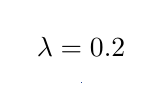
\begin{tikzpicture}[%
font=\footnotesize
]

\begin{axis}[%
width=0.951\figwidth,
height=\figheight,
at={(0\figwidth,0\figheight)},
scale only axis,
xmin=0,
xmax=3,
tick align=outside,
xlabel={Moneyness},
xmajorgrids,
ymin=0,
ymax=5,
ylabel={Remaining Time},
ymajorgrids,
zmin=0,
zmax=200,
zlabel={Optimal Rate},
zmajorgrids,
view={50}{40},
axis background/.style={fill=white},
title style={font=\bfseries},
title={$\lambda = 0.2$},
axis x line*=bottom,
axis y line*=left,
axis z line*=left
]

\addplot3[%
surf,
shader=flat corner,draw=black,z buffer=sort,colormap={mymap}{[1pt] rgb(0pt)=(0.2081,0.1663,0.5292); rgb(1pt)=(0.211624,0.189781,0.577676); rgb(2pt)=(0.212252,0.213771,0.626971); rgb(3pt)=(0.2081,0.2386,0.677086); rgb(4pt)=(0.195905,0.264457,0.7279); rgb(5pt)=(0.170729,0.291938,0.779248); rgb(6pt)=(0.125271,0.324243,0.830271); rgb(7pt)=(0.0591333,0.359833,0.868333); rgb(8pt)=(0.0116952,0.38751,0.881957); rgb(9pt)=(0.00595714,0.408614,0.882843); rgb(10pt)=(0.0165143,0.4266,0.878633); rgb(11pt)=(0.0328524,0.443043,0.871957); rgb(12pt)=(0.0498143,0.458571,0.864057); rgb(13pt)=(0.0629333,0.47369,0.855438); rgb(14pt)=(0.0722667,0.488667,0.8467); rgb(15pt)=(0.0779429,0.503986,0.838371); rgb(16pt)=(0.0793476,0.520024,0.831181); rgb(17pt)=(0.0749429,0.537543,0.826271); rgb(18pt)=(0.0640571,0.556986,0.823957); rgb(19pt)=(0.0487714,0.577224,0.822829); rgb(20pt)=(0.0343429,0.596581,0.819852); rgb(21pt)=(0.0265,0.6137,0.8135); rgb(22pt)=(0.0238905,0.628662,0.803762); rgb(23pt)=(0.0230905,0.641786,0.791267); rgb(24pt)=(0.0227714,0.653486,0.776757); rgb(25pt)=(0.0266619,0.664195,0.760719); rgb(26pt)=(0.0383714,0.674271,0.743552); rgb(27pt)=(0.0589714,0.683757,0.725386); rgb(28pt)=(0.0843,0.692833,0.706167); rgb(29pt)=(0.113295,0.7015,0.685857); rgb(30pt)=(0.145271,0.709757,0.664629); rgb(31pt)=(0.180133,0.717657,0.642433); rgb(32pt)=(0.217829,0.725043,0.619262); rgb(33pt)=(0.258643,0.731714,0.595429); rgb(34pt)=(0.302171,0.737605,0.571186); rgb(35pt)=(0.348167,0.742433,0.547267); rgb(36pt)=(0.395257,0.7459,0.524443); rgb(37pt)=(0.44201,0.748081,0.503314); rgb(38pt)=(0.487124,0.749062,0.483976); rgb(39pt)=(0.530029,0.749114,0.466114); rgb(40pt)=(0.570857,0.748519,0.44939); rgb(41pt)=(0.609852,0.747314,0.433686); rgb(42pt)=(0.6473,0.7456,0.4188); rgb(43pt)=(0.683419,0.743476,0.404433); rgb(44pt)=(0.71841,0.741133,0.390476); rgb(45pt)=(0.752486,0.7384,0.376814); rgb(46pt)=(0.785843,0.735567,0.363271); rgb(47pt)=(0.818505,0.732733,0.34979); rgb(48pt)=(0.850657,0.7299,0.336029); rgb(49pt)=(0.882433,0.727433,0.3217); rgb(50pt)=(0.913933,0.725786,0.306276); rgb(51pt)=(0.944957,0.726114,0.288643); rgb(52pt)=(0.973895,0.731395,0.266648); rgb(53pt)=(0.993771,0.745457,0.240348); rgb(54pt)=(0.999043,0.765314,0.216414); rgb(55pt)=(0.995533,0.786057,0.196652); rgb(56pt)=(0.988,0.8066,0.179367); rgb(57pt)=(0.978857,0.827143,0.163314); rgb(58pt)=(0.9697,0.848138,0.147452); rgb(59pt)=(0.962586,0.870514,0.1309); rgb(60pt)=(0.958871,0.8949,0.113243); rgb(61pt)=(0.959824,0.921833,0.0948381); rgb(62pt)=(0.9661,0.951443,0.0755333); rgb(63pt)=(0.9763,0.9831,0.0538)},mesh/rows=25]
table[row sep=crcr, point meta=\thisrow{c}] {%
%
x	y	z	c\\
0	0.01	1.03013079531058	1.03013079531058\\
0	0.111836734693878	1.19024071779357	1.19024071779357\\
0	0.213673469387755	1.3447525186679	1.3447525186679\\
0	0.315510204081633	1.50983171410871	1.50983171410871\\
0	0.41734693877551	1.68941658633117	1.68941658633117\\
0	0.519183673469388	1.8861889200938	1.8861889200938\\
0	0.621020408163265	2.10257891078855	2.10257891078855\\
0	0.722857142857143	2.34104222093454	2.34104222093454\\
0	0.82469387755102	2.60417644676751	2.60417644676751\\
0	0.926530612244898	2.89478779654435	2.89478779654435\\
0	1.02836734693878	3.21593984827358	3.21593984827358\\
0	1.13020408163265	3.57099594860778	3.57099594860778\\
0	1.23204081632653	3.96366024001922	3.96366024001922\\
0	1.33387755102041	4.3980198253909	4.3980198253909\\
0	1.43571428571429	4.87858954439315	4.87858954439315\\
0	1.53755102040816	5.41036037727834	5.41036037727834\\
0	1.63938775510204	5.99885228724739	5.99885228724739\\
0	1.74122448979592	6.65017223076264	6.65017223076264\\
0	1.8430612244898	7.37107804795024	7.37107804795024\\
0	1.94489795918367	8.16904896534188	8.16904896534188\\
0	2.04673469387755	9.05236348735985	9.05236348735985\\
0	2.14857142857143	10.0301855145286	10.0301855145286\\
0	2.25040816326531	11.1126596022297	11.1126596022297\\
0	2.35224489795918	12.3110163624685	12.3110163624685\\
0	2.45408163265306	13.6376891123029	13.6376891123029\\
0	2.55591836734694	15.106442986525	15.106442986525\\
0	2.65775510204082	16.7325178596548	16.7325178596548\\
0	2.75959183673469	18.5327865643319	18.5327865643319\\
0	2.86142857142857	20.5259300509774	20.5259300509774\\
0	2.96326530612245	22.7326313088184	22.7326313088184\\
0	3.06510204081633	25.1757900625631	25.1757900625631\\
0	3.1669387755102	27.8807604743452	27.8807604743452\\
0	3.26877551020408	30.875614319066	30.875614319066\\
0	3.37061224489796	34.1914323654354	34.1914323654354\\
0	3.47244897959184	37.8626269876889	37.8626269876889\\
0	3.57428571428571	41.9272993569746	41.9272993569746\\
0	3.67612244897959	46.4276349202428	46.4276349202428\\
0	3.77795918367347	51.4103412718105	51.4103412718105\\
0	3.87979591836735	56.9271329628044	56.9271329628044\\
0	3.98163265306122	63.0352682807357	63.0352682807357\\
0	4.0834693877551	69.7981435710009	69.7981435710009\\
0	4.18530612244898	77.2859512691752	77.2859512691752\\
0	4.28714285714286	85.5764084744642	85.5764084744642\\
0	4.38897959183674	94.7555636266212	94.7555636266212\\
0	4.49081632653061	104.918689659451	104.918689659451\\
0	4.59265306122449	116.171272901717	116.171272901717\\
0	4.69448979591837	128.630107989756	128.630107989756\\
0	4.79632653061224	142.42451015679	142.42451015679\\
0	4.89816326530612	157.697657482204	157.697657482204\\
0	5	174.608077032714	174.608077032714\\
0.125	0.01	1.01015054249766	1.01015054249766\\
0.125	0.111836734693878	1.14143044094651	1.14143044094651\\
0.125	0.213673469387755	1.28577503580504	1.28577503580504\\
0.125	0.315510204081633	1.4421540201719	1.4421540201719\\
0.125	0.41734693877551	1.61301802004707	1.61301802004707\\
0.125	0.519183673469388	1.80058158030001	1.80058158030001\\
0.125	0.621020408163265	2.00703356717186	2.00703356717186\\
0.125	0.722857142857143	2.23465823373965	2.23465823373965\\
0.125	0.82469387755102	2.48590463139225	2.48590463139225\\
0.125	0.926530612244898	2.7634349073695	2.7634349073695\\
0.125	1.02836734693878	3.07016427896781	3.07016427896781\\
0.125	1.13020408163265	3.40929837773751	3.40929837773751\\
0.125	1.23204081632653	3.78437080086525	3.78437080086525\\
0.125	1.33387755102041	4.19928248038911	4.19928248038911\\
0.125	1.43571428571429	4.65834392561383	4.65834392561383\\
0.125	1.53755102040816	5.16632113787499	5.16632113787499\\
0.125	1.63938775510204	5.72848588436511	5.72848588436511\\
0.125	1.74122448979592	6.35067097991754	6.35067097991754\\
0.125	1.8430612244898	7.03933122990193	7.03933122990193\\
0.125	1.94489795918367	7.80161071774763	7.80161071774763\\
0.125	2.04673469387755	8.6454171693912	8.6454171693912\\
0.125	2.14857142857143	9.57950418721893	9.57950418721893\\
0.125	2.25040816326531	10.6135622264518	10.6135622264518\\
0.125	2.35224489795918	11.7583190122846	11.7583190122846\\
0.125	2.45408163265306	13.02565221958	13.02565221958\\
0.125	2.55591836734694	14.4287102785204	14.4287102785204\\
0.125	2.65775510204082	15.9820514156895	15.9820514156895\\
0.125	2.75959183673469	17.7017935297493	17.7017935297493\\
0.125	2.86142857142857	19.6057817578278	19.6057817578278\\
0.125	2.96326530612245	21.7137737346384	21.7137737346384\\
0.125	3.06510204081633	24.047644659315	24.047644659315\\
0.125	3.1669387755102	26.6316143743002	26.6316143743002\\
0.125	3.26877551020408	29.4924987623648	29.4924987623648\\
0.125	3.37061224489796	32.6599880907104	32.6599880907104\\
0.125	3.47244897959184	36.1669551887987	36.1669551887987\\
0.125	3.57428571428571	40.0497966590307	40.0497966590307\\
0.125	3.67612244897959	44.3488106621947	44.3488106621947\\
0.125	3.77795918367347	49.1086151991827	49.1086151991827\\
0.125	3.87979591836735	54.3786112307676	54.3786112307676\\
0.125	3.98163265306122	60.213495442607	60.213495442607\\
0.125	4.0834693877551	66.6738279779133	66.6738279779133\\
0.125	4.18530612244898	73.8266610307561	73.8266610307561\\
0.125	4.28714285714286	81.7462348246624	81.7462348246624\\
0.125	4.38897959183674	90.5147482006014	90.5147482006014\\
0.125	4.49081632653061	100.223211812857	100.223211812857\\
0.125	4.59265306122449	110.972392788724	110.972392788724\\
0.125	4.69448979591837	122.873860657321	122.873860657321\\
0.125	4.79632653061224	136.051145348867	136.051145348867\\
0.125	4.89816326530612	150.641019670305	150.641019670305\\
0.125	5	166.794918409223	166.794918409223\\
0.25	0.01	1.01005016975895	1.01005016975895\\
0.25	0.111836734693878	1.12344274943106	1.12344274943106\\
0.25	0.213673469387755	1.2559525317644	1.2559525317644\\
0.25	0.315510204081633	1.40351786693429	1.40351786693429\\
0.25	0.41734693877551	1.56653451373353	1.56653451373353\\
0.25	0.519183673469388	1.74644082575591	1.74644082575591\\
0.25	0.621020408163265	1.94504343495962	1.94504343495962\\
0.25	0.722857142857143	2.16439331881571	2.16439331881571\\
0.25	0.82469387755102	2.40676984005045	2.40676984005045\\
0.25	0.926530612244898	2.67469350809965	2.67469350809965\\
0.25	1.02836734693878	2.97094895332883	2.97094895332883\\
0.25	1.13020408163265	3.29861309316948	3.29861309316948\\
0.25	1.23204081632653	3.66108711795905	3.66108711795905\\
0.25	1.33387755102041	4.0621320660044	4.0621320660044\\
0.25	1.43571428571429	4.50590816416817	4.50590816416817\\
0.25	1.53755102040816	4.9970182802353	4.9970182802353\\
0.25	1.63938775510204	5.54055592321662	5.54055592321662\\
0.25	1.74122448979592	6.14215829142306	6.14215829142306\\
0.25	1.8430612244898	6.8080649253979	6.8080649253979\\
0.25	1.94489795918367	7.54518258242519	7.54518258242519\\
0.25	2.04673469387755	8.36115701021853	8.36115701021853\\
0.25	2.14857142857143	9.26445237345435	9.26445237345435\\
0.25	2.25040816326531	10.2644391592763	10.2644391592763\\
0.25	2.35224489795918	11.3714914785756	11.3714914785756\\
0.25	2.45408163265306	12.5970947754434	12.5970947754434\\
0.25	2.55591836734694	13.9539650648052	13.9539650648052\\
0.25	2.65775510204082	15.4561809396399	15.4561809396399\\
0.25	2.75959183673469	17.1193297038458	17.1193297038458\\
0.25	2.86142857142857	18.9606691945913	18.9606691945913\\
0.25	2.96326530612245	20.9993068977124	20.9993068977124\\
0.25	3.06510204081633	23.2563982927327	23.2563982927327\\
0.25	3.1669387755102	25.7553664406363	25.7553664406363\\
0.25	3.26877551020408	28.5221451093451	28.5221451093451\\
0.25	3.37061224489796	31.5854479585581	31.5854479585581\\
0.25	3.47244897959184	34.9770665782283	34.9770665782283\\
0.25	3.57428571428571	38.7322004743989	38.7322004743989\\
0.25	3.67612244897959	42.8898224276864	42.8898224276864\\
0.25	3.77795918367347	47.4930830168287	47.4930830168287\\
0.25	3.87979591836735	52.5897585062134	52.5897585062134\\
0.25	3.98163265306122	58.2327467463885	58.2327467463885\\
0.25	4.0834693877551	64.4806162349023	64.4806162349023\\
0.25	4.18530612244898	71.3982140365967	71.3982140365967\\
0.25	4.28714285714286	79.0573388734109	79.0573388734109\\
0.25	4.38897959183674	87.5374863701829	87.5374863701829\\
0.25	4.49081632653061	96.9266741918901	96.9266741918901\\
0.25	4.59265306122449	107.32235563701	107.32235563701\\
0.25	4.69448979591837	118.832431169828	118.832431169828\\
0.25	4.79632653061224	131.576368269323	131.576368269323\\
0.25	4.89816326530612	145.686442071938	145.686442071938\\
0.25	5	161.309107122349	161.309107122349\\
0.375	0.01	1.01005016708417	1.01005016708417\\
0.375	0.111836734693878	1.11906901644835	1.11906901644835\\
0.375	0.213673469387755	1.2436057481912	1.2436057481912\\
0.375	0.315510204081633	1.38403181731888	1.38403181731888\\
0.375	0.41734693877551	1.54057106542426	1.54057106542426\\
0.375	0.519183673469388	1.71428068034919	1.71428068034919\\
0.375	0.621020408163265	1.90669686212767	1.90669686212767\\
0.375	0.722857142857143	2.11968048303528	2.11968048303528\\
0.375	0.82469387755102	2.35536662131366	2.35536662131366\\
0.375	0.926530612244898	2.61615630040065	2.61615630040065\\
0.375	1.02836734693878	2.90472715469144	2.90472715469144\\
0.375	1.13020408163265	3.22405410804944	3.22405410804944\\
0.375	1.23204081632653	3.57743651121585	3.57743651121585\\
0.375	1.33387755102041	3.96853033334158	3.96853033334158\\
0.375	1.43571428571429	4.40138493987481	4.40138493987481\\
0.375	1.53755102040816	4.88048443694814	4.88048443694814\\
0.375	1.63938775510204	5.41079380119873	5.41079380119873\\
0.375	1.74122448979592	5.99781015957406	5.99781015957406\\
0.375	1.8430612244898	6.64761968724128	6.64761968724128\\
0.375	1.94489795918367	7.3669606771494	7.3669606771494\\
0.375	2.04673469387755	8.16329341398752	8.16329341398752\\
0.375	2.14857142857143	9.04487756458767	9.04487756458767\\
0.375	2.25040816326531	10.020857879934	10.020857879934\\
0.375	2.35224489795918	11.1013590932655	11.1013590932655\\
0.375	2.45408163265306	12.2975909960757	12.2975909960757\\
0.375	2.55591836734694	13.6219647806131	13.6219647806131\\
0.375	2.65775510204082	15.0882218551549	15.0882218551549\\
0.375	2.75959183673469	16.7115764682528	16.7115764682528\\
0.375	2.86142857142857	18.5088736217826	18.5088736217826\\
0.375	2.96326530612245	20.4987639115123	20.4987639115123\\
0.375	3.06510204081633	22.7018971097355	22.7018971097355\\
0.375	3.1669387755102	25.1411364991346	25.1411364991346\\
0.375	3.26877551020408	27.8417961824867	27.8417961824867\\
0.375	3.37061224489796	30.8319038313412	30.8319038313412\\
0.375	3.47244897959184	34.1424916008734	34.1424916008734\\
0.375	3.57428571428571	37.8079182304886	37.8079182304886\\
0.375	3.67612244897959	41.8662256734597	41.8662256734597\\
0.375	3.77795918367347	46.3595339572915	46.3595339572915\\
0.375	3.87979591836735	51.3344783711761	51.3344783711761\\
0.375	3.98163265306122	56.8426935314093	56.8426935314093\\
0.375	4.0834693877551	62.941349316874	62.941349316874\\
0.375	4.18530612244898	69.6937442798773	69.6937442798773\\
0.375	4.28714285714286	77.1699626606391	77.1699626606391\\
0.375	4.38897959183674	85.4476018371384	85.4476018371384\\
0.375	4.49081632653061	94.6125777590627	94.6125777590627\\
0.375	4.59265306122449	104.76001672601	104.76001672601\\
0.375	4.69448979591837	115.995242766315	115.995242766315\\
0.375	4.79632653061224	128.434870865193	128.434870865193\\
0.375	4.89816326530612	142.208017389539	142.208017389539\\
0.375	5	157.457640273243	157.457640273243\\
0.5	0.01	1.01005016708417	1.01005016708417\\
0.5	0.111836734693878	1.11839740742982	1.11839740742982\\
0.5	0.213673469387755	1.23952581100375	1.23952581100375\\
0.5	0.315510204081633	1.3755075077791	1.3755075077791\\
0.5	0.41734693877551	1.52744776188522	1.52744776188522\\
0.5	0.519183673469388	1.69654601283725	1.69654601283725\\
0.5	0.621020408163265	1.88429916439479	1.88429916439479\\
0.5	0.722857142857143	2.09249124911369	2.09249124911369\\
0.5	0.82469387755102	2.32317697579578	2.32317697579578\\
0.5	0.926530612244898	2.5786801453231	2.5786801453231\\
0.5	1.02836734693878	2.86160411290019	2.86160411290019\\
0.5	1.13020408163265	3.17485071555113	3.17485071555113\\
0.5	1.23204081632653	3.52164551233046	3.52164551233046\\
0.5	1.33387755102041	3.90556825334004	3.90556825334004\\
0.5	1.43571428571429	4.33058813291194	4.33058813291194\\
0.5	1.53755102040816	4.80110375724465	4.80110375724465\\
0.5	1.63938775510204	5.32198798667651	5.32198798667651\\
0.5	1.74122448979592	5.89863796570117	5.89863796570117\\
0.5	1.8430612244898	6.53703076678768	6.53703076678768\\
0.5	1.94489795918367	7.24378516726418	7.24378516726418\\
0.5	2.04673469387755	8.02623016328354	8.02623016328354\\
0.5	2.14857142857143	8.89248090783593	8.89248090783593\\
0.5	2.25040816326531	9.85152284502359	9.85152284502359\\
0.5	2.35224489795918	10.9133049031366	10.9133049031366\\
0.5	2.45408163265306	12.0888427065167	12.0888427065167\\
0.5	2.55591836734694	13.3903328724534	13.3903328724534\\
0.5	2.65775510204082	14.8312795759352	14.8312795759352\\
0.5	2.75959183673469	16.4266346934529	16.4266346934529\\
0.5	2.86142857142857	18.1929529787097	18.1929529787097\\
0.5	2.96326530612245	20.1485638796171	20.1485638796171\\
0.5	3.06510204081633	22.3137617790397	22.3137617790397\\
0.5	3.1669387755102	24.7110166332298	24.7110166332298\\
0.5	3.26877551020408	27.3652071937988	27.3652071937988\\
0.5	3.37061224489796	30.3038792336079	30.3038792336079\\
0.5	3.47244897959184	33.5575314565924	33.5575314565924\\
0.5	3.57428571428571	37.1599320589499	37.1599320589499\\
0.5	3.67612244897959	41.1484692273308	41.1484692273308\\
0.5	3.77795918367347	45.5645392119613	45.5645392119613\\
0.5	3.87979591836735	50.4539760026737	50.4539760026737\\
0.5	3.98163265306122	55.8675270676678	55.8675270676678\\
0.5	4.0834693877551	61.86138009296	61.86138009296\\
0.5	4.18530612244898	68.4977461898604	68.4977461898604\\
0.5	4.28714285714286	75.8455056239494	75.8455056239494\\
0.5	4.38897959183674	83.9809227679846	83.9809227679846\\
0.5	4.49081632653061	92.9884376997009	92.9884376997009\\
0.5	4.59265306122449	102.961542661018	102.961542661018\\
0.5	4.69448979591837	114.00375247601	114.00375247601\\
0.5	4.79632653061224	126.229679000253	126.229679000253\\
0.5	4.89816326530612	139.766220755217	139.766220755217\\
0.5	5	154.753880088677	154.753880088677\\
0.625	0.01	1.01005016708417	1.01005016708417\\
0.625	0.111836734693878	1.11833400392222	1.11833400392222\\
0.625	0.213673469387755	1.23846808113955	1.23846808113955\\
0.625	0.315510204081633	1.37231603419611	1.37231603419611\\
0.625	0.41734693877551	1.52151133706369	1.52151133706369\\
0.625	0.519183673469388	1.68755259366494	1.68755259366494\\
0.625	0.621020408163265	1.87204788437954	1.87204788437954\\
0.625	0.722857142857143	2.07680553408443	2.07680553408443\\
0.625	0.82469387755102	2.30386663405576	2.30386663405576\\
0.625	0.926530612244898	2.55552427633758	2.55552427633758\\
0.625	1.02836734693878	2.83434265903746	2.83434265903746\\
0.625	1.13020408163265	3.14317947508224	3.14317947508224\\
0.625	1.23204081632653	3.48521235884437	3.48521235884437\\
0.625	1.33387755102041	3.86396954993412	3.86396954993412\\
0.625	1.43571428571429	4.28336487019173	4.28336487019173\\
0.625	1.53755102040816	4.74773718310951	4.74773718310951\\
0.625	1.63938775510204	5.26189460104021	5.26189460104021\\
0.625	1.74122448979592	5.83116379740848	5.83116379740848\\
0.625	1.8430612244898	6.46144486549999	6.46144486549999\\
0.625	1.94489795918367	7.15927224486688	7.15927224486688\\
0.625	2.04673469387755	7.93188231434288	7.93188231434288\\
0.625	2.14857142857143	8.78728833004955	8.78728833004955\\
0.625	2.25040816326531	9.73436346996309	9.73436346996309\\
0.625	2.35224489795918	10.7829328355213	10.7829328355213\\
0.625	2.45408163265306	11.9438753570156	11.9438753570156\\
0.625	2.55591836734694	13.2292366546091	13.2292366546091\\
0.625	2.65775510204082	14.6523540221511	14.6523540221511\\
0.625	2.75959183673469	16.2279948279386	16.2279948279386\\
0.625	2.86142857142857	17.9725097666579	17.9725097666579\\
0.625	2.96326530612245	19.9040025514849	19.9040025514849\\
0.625	3.06510204081633	22.0425178063966	22.0425178063966\\
0.625	3.1669387755102	24.4102491079775	24.4102491079775\\
0.625	3.26877551020408	27.0317693353834	27.0317693353834\\
0.625	3.37061224489796	29.9342857188517	29.9342857188517\\
0.625	3.47244897959184	33.1479222336427	33.1479222336427\\
0.625	3.57428571428571	36.7060322702305	36.7060322702305\\
0.625	3.67612244897959	40.6455448258959	40.6455448258959\\
0.625	3.77795918367347	45.007347810875	45.007347810875\\
0.625	3.87979591836735	49.8367124474947	49.8367124474947\\
0.625	3.98163265306122	55.183763167297	55.183763167297\\
0.625	4.0834693877551	61.1039978834316	61.1039978834316\\
0.625	4.18530612244898	67.6588640385005	67.6588640385005\\
0.625	4.28714285714286	74.9163964069826	74.9163964069826\\
0.625	4.38897959183674	82.9519232723734	82.9519232723734\\
0.625	4.49081632653061	91.8488483088956	91.8488483088956\\
0.625	4.59265306122449	101.699516283431	101.699516283431\\
0.625	4.69448979591837	112.606171563356	112.606171563356\\
0.625	4.79632653061224	124.682019379275	124.682019379275\\
0.625	4.89816326530612	138.052400858201	138.052400858201\\
0.625	5	152.85609402364	152.85609402364\\
0.75	0.01	1.01005016708417	1.01005016708417\\
0.75	0.111836734693878	1.11833038694785	1.11833038694785\\
0.75	0.213673469387755	1.23825542916561	1.23825542916561\\
0.75	0.315510204081633	1.37130314693592	1.37130314693592\\
0.75	0.41734693877551	1.51912799243282	1.51912799243282\\
0.75	0.519183673469388	1.68338969229713	1.68338969229713\\
0.75	0.621020408163265	1.8658140934987	1.8658140934987\\
0.75	0.722857142857143	2.06827219948985	2.06827219948985\\
0.75	0.82469387755102	2.29283047498108	2.29283047498108\\
0.75	0.926530612244898	2.54178465950151	2.54178465950151\\
0.75	1.02836734693878	2.81768772236407	2.81768772236407\\
0.75	1.13020408163265	3.12337719964127	3.12337719964127\\
0.75	1.23204081632653	3.4620042972259	3.4620042972259\\
0.75	1.33387755102041	3.83706590755734	3.83706590755734\\
0.75	1.43571428571429	4.2524401938761	4.2524401938761\\
0.75	1.53755102040816	4.71242621938047	4.71242621938047\\
0.75	1.63938775510204	5.22178805640442	5.22178805640442\\
0.75	1.74122448979592	5.78580382635903	5.78580382635903\\
0.75	1.8430612244898	6.41032016312589	6.41032016312589\\
0.75	1.94489795918367	7.10181264804311	7.10181264804311\\
0.75	2.04673469387755	7.86745282866576	7.86745282866576\\
0.75	2.14857142857143	8.71518250456062	8.71518250456062\\
0.75	2.25040816326531	9.65379604141734	9.65379604141734\\
0.75	2.35224489795918	10.6930315602757	10.6930315602757\\
0.75	2.45408163265306	11.8436719425383	11.8436719425383\\
0.75	2.55591836734694	13.1176566946861	13.1176566946861\\
0.75	2.65775510204082	14.5282058303824	14.5282058303824\\
0.75	2.75959183673469	16.0899570531847	16.0899570531847\\
0.75	2.86142857142857	17.819117661752	17.819117661752\\
0.75	2.96326530612245	19.7336327527102	19.7336327527102\\
0.75	3.06510204081633	21.8533714658562	21.8533714658562\\
0.75	3.1669387755102	24.2003332039266	24.2003332039266\\
0.75	3.26877551020408	26.7988759666919	26.7988759666919\\
0.75	3.37061224489796	29.6759691688358	29.6759691688358\\
0.75	3.47244897959184	32.8614735653373	32.8614735653373\\
0.75	3.57428571428571	36.3884511895351	36.3884511895351\\
0.75	3.67612244897959	40.2935085206503	40.2935085206503\\
0.75	3.77795918367347	44.617176442513	44.617176442513\\
0.75	3.87979591836735	49.4043309371647	49.4043309371647\\
0.75	3.98163265306122	54.7046588798594	54.7046588798594\\
0.75	4.0834693877551	60.5731737701544	60.5731737701544\\
0.75	4.18530612244898	67.0707867521219	67.0707867521219\\
0.75	4.28714285714286	74.2649388506187	74.2649388506187\\
0.75	4.38897959183674	82.2303009859641	82.2303009859641\\
0.75	4.49081632653061	91.0495490329109	91.0495490329109\\
0.75	4.59265306122449	100.814221968737	100.814221968737\\
0.75	4.69448979591837	111.625672017729	111.625672017729\\
0.75	4.79632653061224	123.59611665424	123.59611665424\\
0.75	4.89816326530612	136.849803383749	136.849803383749\\
0.75	5	151.52429939198	151.52429939198\\
0.875	0.01	1.01005016708417	1.01005016708417\\
0.875	0.111836734693878	1.11833026372266	1.11833026372266\\
0.875	0.213673469387755	1.23822253966204	1.23822253966204\\
0.875	0.315510204081633	1.37103250941447	1.37103250941447\\
0.875	0.41734693877551	1.51828400895868	1.51828400895868\\
0.875	0.519183673469388	1.68164084981777	1.68164084981777\\
0.875	0.621020408163265	1.86287913086946	1.86287913086946\\
0.875	0.722857142857143	2.06391626116775	2.06391626116775\\
0.875	0.82469387755102	2.28684932095798	2.28684932095798\\
0.875	0.926530612244898	2.53398965578445	2.53398965578445\\
0.875	1.02836734693878	2.80789413397296	2.80789413397296\\
0.875	1.13020408163265	3.11139545421353	3.11139545421353\\
0.875	1.23204081632653	3.44763337816005	3.44763337816005\\
0.875	1.33387755102041	3.8200881336469	3.8200881336469\\
0.875	1.43571428571429	4.23261683731853	4.23261683731853\\
0.875	1.53755102040816	4.68949357924895	4.68949357924895\\
0.875	1.63938775510204	5.19545372228903	5.19545372228903\\
0.875	1.74122448979592	5.75574294519721	5.75574294519721\\
0.875	1.8430612244898	6.37617157262571	6.37617157262571\\
0.875	1.94489795918367	7.06317477166478	7.06317477166478\\
0.875	2.04673469387755	7.82387924621644	7.82387924621644\\
0.875	2.14857142857143	8.66617712326799	8.66617712326799\\
0.875	2.25040816326531	9.59880779758299	9.59880779758299\\
0.875	2.35224489795918	10.6314485829924	10.6314485829924\\
0.875	2.45408163265306	11.7748151095767	11.7748151095767\\
0.875	2.55591836734694	13.0407725071951	13.0407725071951\\
0.875	2.65775510204082	14.442458527921	14.442458527921\\
0.875	2.75959183673469	15.9944198840567	15.9944198840567\\
0.875	2.86142857142857	17.7127632157711	17.7127632157711\\
0.875	2.96326530612245	19.6153222544378	19.6153222544378\\
0.875	3.06510204081633	21.7218429160187	21.7218429160187\\
0.875	3.1669387755102	24.0541882450795	24.0541882450795\\
0.875	3.26877551020408	26.6365653361857	26.6365653361857\\
0.875	3.37061224489796	29.4957765876349	29.4957765876349\\
0.875	3.47244897959184	32.6614978951249	32.6614978951249\\
0.875	3.57428571428571	36.166586672644	36.166586672644\\
0.875	3.67612244897959	40.0474228975222	40.0474228975222\\
0.875	3.77795918367347	44.3442867194003	44.3442867194003\\
0.875	3.87979591836735	49.1017765524313	49.1017765524313\\
0.875	3.98163265306122	54.3692719902607	54.3692719902607\\
0.875	4.0834693877551	60.2014463485963	60.2014463485963\\
0.875	4.18530612244898	66.6588341553204	66.6588341553204\\
0.875	4.28714285714286	73.8084594784468	73.8084594784468\\
0.875	4.38897959183674	81.7245316137138	81.7245316137138\\
0.875	4.49081632653061	90.4892153527907	90.4892153527907\\
0.875	4.59265306122449	100.193483827202	100.193483827202\\
0.875	4.69448979591837	110.93806278019	110.93806278019\\
0.875	4.79632653061224	122.834476067742	122.834476067742\\
0.875	4.89816326530612	136.00620324073	136.00620324073\\
0.875	5	150.589961223484	150.589961223484\\
1	0.01	1.01005016708417	1.01005016708417\\
1	0.111836734693878	1.11833026123665	1.11833026123665\\
1	0.213673469387755	1.23821864857476	1.23821864857476\\
1	0.315510204081633	1.37097193203043	1.37097193203043\\
1	0.41734693877551	1.51802161239119	1.51802161239119\\
1	0.519183673469388	1.68097697614919	1.68097697614919\\
1	0.621020408163265	1.86160587529025	1.86160587529025\\
1	0.722857142857143	2.06183821521286	2.06183821521286\\
1	0.82469387755102	2.2837871481141	2.2837871481141\\
1	0.926530612244898	2.52977655935527	2.52977655935527\\
1	1.02836734693878	2.80237033296229	2.80237033296229\\
1	1.13020408163265	3.10440266566404	3.10440266566404\\
1	1.23204081632653	3.43900990092461	3.43900990092461\\
1	1.33387755102041	3.80966458576507	3.80966458576507\\
1	1.43571428571429	4.22021242190028	4.22021242190028\\
1	1.53755102040816	4.67491271738767	4.67491271738767\\
1	1.63938775510204	5.17848290313299	5.17848290313299\\
1	1.74122448979592	5.73614766685869	5.73614766685869\\
1	1.8430612244898	6.35369327029459	6.35369327029459\\
1	1.94489795918367	7.03752764740118	7.03752764740118\\
1	2.04673469387755	7.79474692802984	7.79474692802984\\
1	2.14857142857143	8.6332090899037	8.6332090899037\\
1	2.25040816326531	9.56161551077703	9.56161551077703\\
1	2.35224489795918	10.5896012715784	10.5896012715784\\
1	2.45408163265306	11.7278351503204	11.7278351503204\\
1	2.55591836734694	12.9881303460284	12.9881303460284\\
1	2.65775510204082	14.3835670826425	14.3835670826425\\
1	2.75959183673469	15.9286283657685	15.9286283657685\\
1	2.86142857142857	17.6393503014462	17.6393503014462\\
1	2.96326530612245	19.533488537132	19.533488537132\\
1	3.06510204081633	21.6307025523738	21.6307025523738\\
1	3.1669387755102	23.9527597119043	23.9527597119043\\
1	3.26877551020408	26.5237611990028	26.5237611990028\\
1	3.37061224489796	29.3703921740916	29.3703921740916\\
1	3.47244897959184	32.5221987549972	32.5221987549972\\
1	3.57428571428571	36.0118946937204	36.0118946937204\\
1	3.67612244897959	39.8757009328166	39.8757009328166\\
1	3.77795918367347	44.1537215657809	44.1537215657809\\
1	3.87979591836735	48.8903601037095	48.8903601037095\\
1	3.98163265306122	54.1347803688864	54.1347803688864\\
1	4.0834693877551	59.9414167991687	59.9414167991687\\
1	4.18530612244898	66.3705394599219	66.3705394599219\\
1	4.28714285714286	73.4888796281107	73.4888796281107\\
1	4.38897959183674	81.3703224418788	81.3703224418788\\
1	4.49081632653061	90.0966738050741	90.0966738050741\\
1	4.59265306122449	99.7585095069254	99.7585095069254\\
1	4.69448979591837	110.456115370445	110.456115370445\\
1	4.79632653061224	122.300528187987	122.300528187987\\
1	4.89816326530612	135.414688248541	135.414688248541\\
1	5	149.934715419602	149.934715419602\\
1.125	0.01	1.01005016708417	1.01005016708417\\
1.125	0.111836734693878	1.11833026120714	1.11833026120714\\
1.125	0.213673469387755	1.2382182978988	1.2382182978988\\
1.125	0.315510204081633	1.37096061495753	1.37096061495753\\
1.125	0.41734693877551	1.51795023662821	1.51795023662821\\
1.125	0.519183673469388	1.68075002017074	1.68075002017074\\
1.125	0.621020408163265	1.86109856921436	1.86109856921436\\
1.125	0.722857142857143	2.06091468317574	2.06091468317574\\
1.125	0.82469387755102	2.28231076278004	2.28231076278004\\
1.125	0.926530612244898	2.52761376809587	2.52761376809587\\
1.125	1.02836734693878	2.79939074261391	2.79939074261391\\
1.125	1.13020408163265	3.10047735018102	3.10047735018102\\
1.125	1.23204081632653	3.43400900816194	3.43400900816194\\
1.125	1.33387755102041	3.80345475698339	3.80345475698339\\
1.125	1.43571428571429	4.21265423475998	4.21265423475998\\
1.125	1.53755102040816	4.66585821362226	4.66585821362226\\
1.125	1.63938775510204	5.16777319336924	5.16777319336924\\
1.125	1.74122448979592	5.72361057641969	5.72361057641969\\
1.125	1.8430612244898	6.33914098002387	6.33914098002387\\
1.125	1.94489795918367	7.02075428195347	7.02075428195347\\
1.125	2.04673469387755	7.77552604554581	7.77552604554581\\
1.125	2.14857142857143	8.61129102913118	8.61129102913118\\
1.125	2.25040816326531	9.5367245534733	9.5367245534733\\
1.125	2.35224489795918	10.5614325790208	10.5614325790208\\
1.125	2.45408163265306	11.6960514328519	11.6960514328519\\
1.125	2.55591836734694	12.9523582237743	12.9523582237743\\
1.125	2.65775510204082	14.3433930939084	14.3433930939084\\
1.125	2.75959183673469	15.8835945772089	15.8835945772089\\
1.125	2.86142857142857	17.5889494709309	17.5889494709309\\
1.125	2.96326530612245	19.4771587763468	19.4771587763468\\
1.125	3.06510204081633	21.5678214315872	21.5678214315872\\
1.125	3.1669387755102	23.8826377439967	23.8826377439967\\
1.125	3.26877551020408	26.4456346337677	26.4456346337677\\
1.125	3.37061224489796	29.2834150269359	29.2834150269359\\
1.125	3.47244897959184	32.4254339864388	32.4254339864388\\
1.125	3.57428571428571	35.9043044474351	35.9043044474351\\
1.125	3.67612244897959	39.7561357303509	39.7561357303509\\
1.125	3.77795918367347	44.0209083453209	44.0209083453209\\
1.125	3.87979591836735	48.7428889783839	48.7428889783839\\
1.125	3.98163265306122	53.9710899668552	53.9710899668552\\
1.125	4.0834693877551	59.7597780330838	59.7597780330838\\
1.125	4.18530612244898	66.169037557084	66.169037557084\\
1.125	4.28714285714286	73.2653942346299	73.2653942346299\\
1.125	4.38897959183674	81.1225055941803	81.1225055941803\\
1.125	4.49081632653061	89.8219255399787	89.8219255399787\\
1.125	4.59265306122449	99.4539508570402	99.4539508570402\\
1.125	4.69448979591837	110.118558464477	110.118558464477\\
1.125	4.79632653061224	121.926443145557	121.926443145557\\
1.125	4.89816326530612	135.000166525795	135.000166525795\\
1.125	5	149.475429225126	149.475429225126\\
1.25	0.01	1.01005016708417	1.01005016708417\\
1.25	0.111836734693878	1.11833026120693	1.11833026120693\\
1.25	0.213673469387755	1.23821827389931	1.23821827389931\\
1.25	0.315510204081633	1.37095885517461	1.37095885517461\\
1.25	0.41734693877551	1.51793329463881	1.51793329463881\\
1.25	0.519183673469388	1.6806803263921	1.6806803263921\\
1.25	0.621020408163265	1.86091340684496	1.86091340684496\\
1.25	0.722857142857143	2.06053329412758	2.06053329412758\\
1.25	0.82469387755102	2.28164210907953	2.28164210907953\\
1.25	0.926530612244898	2.52656186705801	2.52656186705801\\
1.25	1.02836734693878	2.79785742357711	2.79785742357711\\
1.25	1.13020408163265	3.09836314303812	3.09836314303812\\
1.25	1.23204081632653	3.43121287147762	3.43121287147762\\
1.25	1.33387755102041	3.79987314551992	3.79987314551992\\
1.25	1.43571428571429	4.20817981249194	4.20817981249194\\
1.25	1.53755102040816	4.66037838272543	4.66037838272543\\
1.25	1.63938775510204	5.16116852482439	5.16116852482439\\
1.25	1.74122448979592	5.71575317781193	5.71575317781193\\
1.25	1.8430612244898	6.3298928076603	6.3298928076603\\
1.25	1.94489795918367	7.00996538867569	7.00996538867569\\
1.25	2.04673469387755	7.76303274706072	7.76303274706072\\
1.25	2.14857142857143	8.59691396704124	8.59691396704124\\
1.25	2.25040816326531	9.52026663055311	9.52026663055311\\
1.25	2.35224489795918	10.5426767405744	10.5426767405744\\
1.25	2.45408163265306	11.6747582665843	11.6747582665843\\
1.25	2.55591836734694	12.9282633491806	12.9282633491806\\
1.25	2.65775510204082	14.3162043105374	14.3162043105374\\
1.25	2.75959183673469	15.8529887391887	15.8529887391887\\
1.25	2.86142857142857	17.5545690527898	17.5545690527898\\
1.25	2.96326530612245	19.438608092389	19.438608092389\\
1.25	3.06510204081633	21.5246624678481	21.5246624678481\\
1.25	3.1669387755102	23.8343855580896	23.8343855580896\\
1.25	3.26877551020408	26.3917522737013	26.3917522737013\\
1.25	3.37061224489796	29.223307915198	29.223307915198\\
1.25	3.47244897959184	32.3584437102611	32.3584437102611\\
1.25	3.57428571428571	35.8297018901338	35.8297018901338\\
1.25	3.67612244897959	39.6731134719078	39.6731134719078\\
1.25	3.77795918367347	43.9285722528823	43.9285722528823\\
1.25	3.87979591836735	48.6402488990189	48.6402488990189\\
1.25	3.98163265306122	53.8570494256616	53.8570494256616\\
1.25	4.0834693877551	59.6331228294543	59.6331228294543\\
1.25	4.18530612244898	66.0284231405512	66.0284231405512\\
1.25	4.28714285714286	73.1093317290758	73.1093317290758\\
1.25	4.38897959183674	80.9493463251932	80.9493463251932\\
1.25	4.49081632653061	89.6298439046281	89.6298439046281\\
1.25	4.59265306122449	99.2409253581531	99.2409253581531\\
1.25	4.69448979591837	109.882350712464	109.882350712464\\
1.25	4.79632653061224	121.664574609752	121.664574609752\\
1.25	4.89816326530612	134.709892793929	134.709892793929\\
1.25	5	149.153711503688	149.153711503688\\
1.375	0.01	1.01005016708417	1.01005016708417\\
1.375	0.111836734693878	1.11833026120693	1.11833026120693\\
1.375	0.213673469387755	1.23821827265507	1.23821827265507\\
1.375	0.315510204081633	1.37095862789302	1.37095862789302\\
1.375	0.41734693877551	1.51792979265606	1.51792979265606\\
1.375	0.519183673469388	1.68066114118543	1.68066114118543\\
1.375	0.621020408163265	1.86085162128362	1.86085162128362\\
1.375	0.722857142857143	2.06038723659291	2.06038723659291\\
1.375	0.82469387755102	2.28135821835064	2.28135821835064\\
1.375	0.926530612244898	2.52607814281201	2.52607814281201\\
1.375	1.02836734693878	2.79710617612934	2.79710617612934\\
1.375	1.13020408163265	3.09727272995091	3.09727272995091\\
1.375	1.23204081632653	3.42970853552278	3.42970853552278\\
1.375	1.33387755102041	3.79787717798915	3.79787717798915\\
1.375	1.43571428571429	4.2056112479418	4.2056112479418\\
1.375	1.53755102040816	4.65715237919872	4.65715237919872\\
1.375	1.63938775510204	5.15719553295786	5.15719553295786\\
1.375	1.74122448979592	5.71093796281384	5.71093796281384\\
1.375	1.8430612244898	6.32413336018571	6.32413336018571\\
1.375	1.94489795918367	7.00315174171112	7.00315174171112\\
1.375	2.04673469387755	7.75504570341588	7.75504570341588\\
1.375	2.14857142857143	8.58762373380693	8.58762373380693\\
1.375	2.25040816326531	9.50953135138654	9.50953135138654\\
1.375	2.35224489795918	10.5303409128678	10.5303409128678\\
1.375	2.45408163265306	11.6606510277642	11.6606510277642\\
1.375	2.55591836734694	12.9121966141185	12.9121966141185\\
1.375	2.65775510204082	14.2979707400319	14.2979707400319\\
1.375	2.75959183673469	15.8323595175108	15.8323595175108\\
1.375	2.86142857142857	17.5312914502401	17.5312914502401\\
1.375	2.96326530612245	19.4124027866055	19.4124027866055\\
1.375	3.06510204081633	21.4952205951695	21.4952205951695\\
1.375	3.1669387755102	23.8013654635624	23.8013654635624\\
1.375	3.26877551020408	26.354775925287	26.354775925287\\
1.375	3.37061224489796	29.1819569443392	29.1819569443392\\
1.375	3.47244897959184	32.3122550371739	32.3122550371739\\
1.375	3.57428571428571	35.778162887957	35.778162887957\\
1.375	3.67612244897959	39.6156566191211	39.6156566191211\\
1.375	3.77795918367347	43.8645692181508	43.8645692181508\\
1.375	3.87979591836735	48.5690039967805	48.5690039967805\\
1.375	3.98163265306122	53.7777923742843	53.7777923742843\\
1.375	4.0834693877551	59.5450007365892	59.5450007365892\\
1.375	4.18530612244898	65.930491632314	65.930491632314\\
1.375	4.28714285714286	73.00054513083	73.00054513083\\
1.375	4.38897959183674	80.8285467918865	80.8285467918865\\
1.375	4.49081632653061	89.4957493877475	89.4957493877475\\
1.375	4.59265306122449	99.0921162843061	99.0921162843061\\
1.375	4.69448979591837	109.717255235231	109.717255235231\\
1.375	4.79632653061224	121.48145228166	121.48145228166\\
1.375	4.89816326530612	134.506816489005	134.506816489005\\
1.375	5	148.928547402903	148.928547402903\\
1.5	0.01	1.01005016708417	1.01005016708417\\
1.5	0.111836734693878	1.11833026120693	1.11833026120693\\
1.5	0.213673469387755	1.23821827260629	1.23821827260629\\
1.5	0.315510204081633	1.37095860355261	1.37095860355261\\
1.5	0.41734693877551	1.51792916328538	1.51792916328538\\
1.5	0.519183673469388	1.68065641436235	1.68065641436235\\
1.5	0.621020408163265	1.8608328031119	1.8608328031119\\
1.5	0.722857142857143	2.06033545031002	2.06033545031002\\
1.5	0.82469387755102	2.28124541148257	2.28124541148257\\
1.5	0.926530612244898	2.52586817107379	2.52586817107379\\
1.5	1.02836734693878	2.79675632880922	2.79675632880922\\
1.5	1.13020408163265	3.09673511504168	3.09673511504168\\
1.5	1.23204081632653	3.4289310874496	3.4289310874496\\
1.5	1.33387755102041	3.79680425041294	3.79680425041294\\
1.5	1.43571428571429	4.20418383986964	4.20418383986964\\
1.5	1.53755102040816	4.65530806579051	4.65530806579051\\
1.5	1.63938775510204	5.1548681678292	5.1548681678292\\
1.5	1.74122448979592	5.70805720470069	5.70805720470069\\
1.5	1.8430612244898	6.32062406182676	6.32062406182676\\
1.5	1.94489795918367	6.99893322578824	6.99893322578824\\
1.5	2.04673469387755	7.75003094008156	7.75003094008156\\
1.5	2.14857142857143	8.58171842649606	8.58171842649606\\
1.5	2.25040816326531	9.50263293175641	9.50263293175641\\
1.5	2.35224489795918	10.5223374413182	10.5223374413182\\
1.5	2.45408163265306	11.6514199926228	11.6514199926228\\
1.5	2.55591836734694	12.9016036198949	12.9016036198949\\
1.5	2.65775510204082	14.2858680728926	14.2858680728926\\
1.5	2.75959183673469	15.8185845741206	15.8185845741206\\
1.5	2.86142857142857	17.5156650142153	17.5156650142153\\
1.5	2.96326530612245	19.3947271349329	19.3947271349329\\
1.5	3.06510204081633	21.475277414985	21.475277414985\\
1.5	3.1669387755102	23.778913557598	23.778913557598\\
1.5	3.26877551020408	26.3295486820314	26.3295486820314\\
1.5	3.37061224489796	29.1536595464853	29.1536595464853\\
1.5	3.47244897959184	32.2805613791937	32.2805613791937\\
1.5	3.57428571428571	35.7427121706274	35.7427121706274\\
1.5	3.67612244897959	39.5760495854783	39.5760495854783\\
1.5	3.77795918367347	43.8203639916417	43.8203639916417\\
1.5	3.87979591836735	48.5197114782657	48.5197114782657\\
1.5	3.98163265306122	53.722871149981	53.722871149981\\
1.5	4.0834693877551	59.4838514439813	59.4838514439813\\
1.5	4.18530612244898	65.8624507254463	65.8624507254463\\
1.5	4.28714285714286	72.9248779801786	72.9248779801786\\
1.5	4.38897959183674	80.7444400471032	80.7444400471032\\
1.5	4.49081632653061	89.4023025239358	89.4023025239358\\
1.5	4.59265306122449	98.9883322440195	98.9883322440195\\
1.5	4.69448979591837	109.602030069007	109.602030069007\\
1.5	4.79632653061224	121.353563679511	121.353563679511\\
1.5	4.89816326530612	134.364911083793	134.364911083793\\
1.5	5	148.77112671377	148.77112671377\\
1.625	0.01	1.01005016708417	1.01005016708417\\
1.625	0.111836734693878	1.11833026120693	1.11833026120693\\
1.625	0.213673469387755	1.23821827260485	1.23821827260485\\
1.625	0.315510204081633	1.37095860139401	1.37095860139401\\
1.625	0.41734693877551	1.5179290650674	1.5179290650674\\
1.625	0.519183673469388	1.68065537335631	1.68065537335631\\
1.625	0.621020408163265	1.86082757833971	1.86082757833971\\
1.625	0.722857142857143	2.06031847283942	2.06031847283942\\
1.625	0.82469387755102	2.28120351528164	2.28120351528164\\
1.625	0.926530612244898	2.52578225540476	2.52578225540476\\
1.625	1.02836734693878	2.79660169058594	2.79660169058594\\
1.625	1.13020408163265	3.09648208229303	3.09648208229303\\
1.625	1.23204081632653	3.42854568077773	3.42854568077773\\
1.625	1.33387755102041	3.79624872317541	3.79624872317541\\
1.625	1.43571428571429	4.20341703774749	4.20341703774749\\
1.625	1.53755102040816	4.65428559749946	4.65428559749946\\
1.625	1.63938775510204	5.15354240230583	5.15354240230583\\
1.625	1.74122448979592	5.70637711768152	5.70637711768152\\
1.625	1.8430612244898	6.31853495427901	6.31853495427901\\
1.625	1.94489795918367	6.99637633278157	6.99637633278157\\
1.625	2.04673469387755	7.74694294382748	7.74694294382748\\
1.625	2.14857142857143	8.57803088254814	8.57803088254814\\
1.625	2.25040816326531	9.49827161318878	9.49827161318878\\
1.625	2.35224489795918	10.5172216021735	10.5172216021735\\
1.625	2.45408163265306	11.6454615489841	11.6454615489841\\
1.625	2.55591836734694	12.8947062444772	12.8947062444772\\
1.625	2.65775510204082	14.2779261969466	14.2779261969466\\
1.625	2.75959183673469	15.8094822885854	15.8094822885854\\
1.625	2.86142857142857	17.5052748603555	17.5052748603555\\
1.625	2.96326530612245	19.3829087730674	19.3829087730674\\
1.625	3.06510204081633	21.4618761583042	21.4618761583042\\
1.625	3.1669387755102	23.7637587564129	23.7637587564129\\
1.625	3.26877551020408	26.3124519420696	26.3124519420696\\
1.625	3.37061224489796	29.1344127629951	29.1344127629951\\
1.625	3.47244897959184	32.2589345666179	32.2589345666179\\
1.625	3.57428571428571	35.7184510654219	35.7184510654219\\
1.625	3.67612244897959	39.5488729972525	39.5488729972525\\
1.625	3.77795918367347	43.7899608751562	43.7899608751562\\
1.625	3.87979591836735	48.4857376959022	48.4857376959022\\
1.625	3.98163265306122	53.6849458910782	53.6849458910782\\
1.625	4.0834693877551	59.4415532638573	59.4415532638573\\
1.625	4.18530612244898	65.8153131629762	65.8153131629762\\
1.625	4.28714285714286	72.8723847084207	72.8723847084207\\
1.625	4.38897959183674	80.686019506618	80.686019506618\\
1.625	4.49081632653061	89.337321983074	89.337321983074\\
1.625	4.59265306122449	98.916091224506	98.916091224506\\
1.625	4.69448979591837	109.521753068564	109.521753068564\\
1.625	4.79632653061224	121.264392115966	121.264392115966\\
1.625	4.89816326530612	134.26589437704	134.26589437704\\
1.625	5	148.661212412999	148.661212412999\\
1.75	0.01	1.01005016708417	1.01005016708417\\
1.75	0.111836734693878	1.11833026120693	1.11833026120693\\
1.75	0.213673469387755	1.23821827260482	1.23821827260482\\
1.75	0.315510204081633	1.37095860123565	1.37095860123565\\
1.75	0.41734693877551	1.51792905177134	1.51792905177134\\
1.75	0.519183673469388	1.68065516862921	1.68065516862921\\
1.75	0.621020408163265	1.86082625732725	1.86082625732725\\
1.75	0.722857142857143	2.06031333195257	2.06031333195257\\
1.75	0.82469387755102	2.28118898762732	2.28118898762732\\
1.75	0.926530612244898	2.52574915397852	2.52574915397852\\
1.75	1.02836734693878	2.79653688688444	2.79653688688444\\
1.75	1.13020408163265	3.09636852950489	3.09636852950489\\
1.75	1.23204081632653	3.42836263123879	3.42836263123879\\
1.75	1.33387755102041	3.79597200989928	3.79597200989928\\
1.75	1.43571428571429	4.20301933301409	4.20301933301409\\
1.75	1.53755102040816	4.65373660043586	4.65373660043586\\
1.75	1.63938775510204	5.15280893451256	5.15280893451256\\
1.75	1.74122448979592	5.70542312206067	5.70542312206067\\
1.75	1.8430612244898	6.31732140040285	6.31732140040285\\
1.75	1.94489795918367	6.99486103534611	6.99486103534611\\
1.75	2.04673469387755	7.74508030111302	7.74508030111302\\
1.75	2.14857142857143	8.57577154073872	8.57577154073872\\
1.75	2.25040816326531	9.49556206070014	9.49556206070014\\
1.75	2.35224489795918	10.5140036962476	10.5140036962476\\
1.75	2.45408163265306	11.641671974947	11.641671974947\\
1.75	2.55591836734694	12.8902759063163	12.8902759063163\\
1.75	2.65775510204082	14.2727795362618	14.2727795362618\\
1.75	2.75959183673469	15.803536527496	15.803536527496\\
1.75	2.86142857142857	17.4984391625662	17.4984391625662\\
1.75	2.96326530612245	19.3750833159809	19.3750833159809\\
1.75	3.06510204081633	21.4529511077796	21.4529511077796\\
1.75	3.1669387755102	23.7536131344745	23.7536131344745\\
1.75	3.26877551020408	26.3009523765372	26.3009523765372\\
1.75	3.37061224489796	29.121412106615	29.121412106615\\
1.75	3.47244897959184	32.2442703717861	32.2442703717861\\
1.75	3.57428571428571	35.7019438989943	35.7019438989943\\
1.75	3.67612244897959	39.5303245781995	39.5303245781995\\
1.75	3.77795918367347	43.7691520159212	43.7691520159212\\
1.75	3.87979591836735	48.4624260262449	48.4624260262449\\
1.75	3.98163265306122	53.6588633408873	53.6588633408873\\
1.75	4.0834693877551	59.4124032788921	59.4124032788921\\
1.75	4.18530612244898	65.7827676247051	65.7827676247051\\
1.75	4.28714285714286	72.8360805260361	72.8360805260361\\
1.75	4.38897959183674	80.6455548458953	80.6455548458953\\
1.75	4.49081632653061	89.2922520929609	89.2922520929609\\
1.75	4.59265306122449	98.8659238181511	98.8659238181511\\
1.75	4.69448979591837	109.465943210858	109.465943210858\\
1.75	4.79632653061224	121.202336564549	121.202336564549\\
1.75	4.89816326530612	134.196925318043	134.196925318043\\
1.75	5	148.584590526519	148.584590526519\\
1.875	0.01	1.01005016708417	1.01005016708417\\
1.875	0.111836734693878	1.11833026120693	1.11833026120693\\
1.875	0.213673469387755	1.23821827260482	1.23821827260482\\
1.875	0.315510204081633	1.37095860122605	1.37095860122605\\
1.875	0.41734693877551	1.51792905021129	1.51792905021129\\
1.875	0.519183673469388	1.68065513270607	1.68065513270607\\
1.875	0.621020408163265	1.86082595342852	1.86082595342852\\
1.875	0.722857142857143	2.06031189536214	2.06031189536214\\
1.875	0.82469387755102	2.28118428858238	2.28118428858238\\
1.875	0.926530612244898	2.52573715669233	2.52573715669233\\
1.875	1.02836734693878	2.79651116432209	2.79651116432209\\
1.875	1.13020408163265	3.09631998844032	3.09631998844032\\
1.875	1.23204081632653	3.42827941978007	3.42827941978007\\
1.875	1.33387755102041	3.79583954599188	3.79583954599188\\
1.875	1.43571428571429	4.20282039183837	4.20282039183837\\
1.875	1.53755102040816	4.65345141212892	4.65345141212892\\
1.875	1.63938775510204	5.1524152595735	5.1524152595735\\
1.875	1.74122448979592	5.7048962850972	5.7048962850972\\
1.875	1.8430612244898	6.31663427229793	6.31663427229793\\
1.875	1.94489795918367	6.99398395985142	6.99398395985142\\
1.875	2.04673469387755	7.74398096517491	7.74398096517491\\
1.875	2.14857142857143	8.57441478937201	8.57441478937201\\
1.875	2.25040816326531	9.49390965760264	9.49390965760264\\
1.875	2.35224489795918	10.5120140310546	10.5120140310546\\
1.875	2.45408163265306	11.6392997173604	11.6392997173604\\
1.875	2.55591836734694	12.8874716064918	12.8874716064918\\
1.875	2.65775510204082	14.269489169906	14.269489169906\\
1.875	2.75959183673469	15.7997009831672	15.7997009831672\\
1.875	2.86142857142857	17.4939936677131	17.4939936677131\\
1.875	2.96326530612245	19.3699567972992	19.3699567972992\\
1.875	3.06510204081633	21.4470654805073	21.4470654805073\\
1.875	3.1669387755102	23.7468825142786	23.7468825142786\\
1.875	3.26877551020408	26.2932822066487	26.2932822066487\\
1.875	3.37061224489796	29.1126981918291	29.1126981918291\\
1.875	3.47244897959184	32.2343978098518	32.2343978098518\\
1.875	3.57428571428571	35.6907858987452	35.6907858987452\\
1.875	3.67612244897959	39.5177411525197	39.5177411525197\\
1.875	3.77795918367347	43.7549885362721	43.7549885362721\\
1.875	3.87979591836735	48.4465116239873	48.4465116239873\\
1.875	3.98163265306122	53.6410091389979	53.6410091389979\\
1.875	4.0834693877551	59.3924004358806	59.3924004358806\\
1.875	4.18530612244898	65.7603851705571	65.7603851705571\\
1.875	4.28714285714286	72.811062967827	72.811062967827\\
1.875	4.38897959183674	80.6176195183115	80.6176195183115\\
1.875	4.49081632653061	89.2610862263017	89.2610862263017\\
1.875	4.59265306122449	98.8311812934389	98.8311812934389\\
1.875	4.69448979591837	109.427240968429	109.427240968429\\
1.875	4.79632653061224	121.159250628891	121.159250628891\\
1.875	4.89816326530612	134.148986397656	134.148986397656\\
1.875	5	148.531279143156	148.531279143156\\
2	0.01	1.01005016708417	1.01005016708417\\
2	0.111836734693878	1.11833026120693	1.11833026120693\\
2	0.213673469387755	1.23821827260482	1.23821827260482\\
2	0.315510204081633	1.37095860122557	1.37095860122557\\
2	0.41734693877551	1.51792905005275	1.51792905005275\\
2	0.519183673469388	1.68065512708586	1.68065512708586\\
2	0.621020408163265	1.86082588986168	1.86082588986168\\
2	0.722857142857143	2.06031152515335	2.06031152515335\\
2	0.82469387755102	2.28118287182453	2.28118287182453\\
2	0.926530612244898	2.52573306927737	2.52573306927737\\
2	1.02836734693878	2.79650150123564	2.79650150123564\\
2	1.13020408163265	3.09630023897464	3.09630023897464\\
2	1.23204081632653	3.42824324586237	3.42824324586237\\
2	1.33387755102041	3.7957786582103	3.7957786582103\\
2	1.43571428571429	4.2027244987726	4.2027244987726\\
2	1.53755102040816	4.65330821377099	4.65330821377099\\
2	1.63938775510204	5.15221045859296	5.15221045859296\\
2	1.74122448979592	5.70461359557476	5.70461359557476\\
2	1.8430612244898	6.31625541156899	6.31625541156899\\
2	1.94489795918367	6.99348861408139	6.99348861408139\\
2	2.04673469387755	7.74334672293275	7.74334672293275\\
2	2.14857142857143	8.5736170398883	8.5736170398883\\
2	2.25040816326531	9.49292145184313	9.49292145184313\\
2	2.35224489795918	10.5108059044695	10.5108059044695\\
2	2.45408163265306	11.6378394734015	11.6378394734015\\
2	2.55591836734694	12.8857240598895	12.8857240598895\\
2	2.65775510204082	14.267415848385	14.267415848385\\
2	2.75959183673469	15.7972597858275	15.7972597858275\\
2	2.86142857142857	17.491138477768	17.491138477768\\
2	2.96326530612245	19.3666370462685	19.3666370462685\\
2	3.06510204081633	21.4432256603285	21.4432256603285\\
2	3.1669387755102	23.7424616331306	23.7424616331306\\
2	3.26877551020408	26.2882131835767	26.2882131835767\\
2	3.37061224489796	29.1069071845168	29.1069071845168\\
2	3.47244897959184	32.2278034690974	32.2278034690974\\
2	3.57428571428571	35.6832985423537	35.6832985423537\\
2	3.67612244897959	39.5092618504184	39.5092618504184\\
2	3.77795918367347	43.7454080976736	43.7454080976736\\
2	3.87979591836735	48.4357094763568	48.4357094763568\\
2	3.98163265306122	53.6288520874184	53.6288520874184\\
2	4.0834693877551	59.3787412901298	59.3787412901298\\
2	4.18530612244898	65.7450612258089	65.7450612258089\\
2	4.28714285714286	72.7938943233462	72.7938943233462\\
2	4.38897959183674	80.5984072168077	80.5984072168077\\
2	4.49081632653061	89.2396101947294	89.2396101947294\\
2	4.59265306122449	98.8071980639565	98.8071980639565\\
2	4.69448979591837	109.400481155935	109.400481155935\\
2	4.79632653061224	121.129416139015	121.129416139015\\
2	4.89816326530612	134.115747336291	134.115747336291\\
2	5	148.494270395483	148.494270395483\\
2.125	0.01	1.01005016708417	1.01005016708417\\
2.125	0.111836734693878	1.11833026120693	1.11833026120693\\
2.125	0.213673469387755	1.23821827260482	1.23821827260482\\
2.125	0.315510204081633	1.37095860122555	1.37095860122555\\
2.125	0.41734693877551	1.5179290500388	1.5179290500388\\
2.125	0.519183673469388	1.68065512630232	1.68065512630232\\
2.125	0.621020408163265	1.86082587777909	1.86082587777909\\
2.125	0.722857142857143	2.0603114372267	2.0603114372267\\
2.125	0.82469387755102	2.28118247391357	2.28118247391357\\
2.125	0.926530612244898	2.52573176110131	2.52573176110131\\
2.125	1.02836734693878	2.7964980678979	2.7964980678979\\
2.125	1.13020408163265	3.09629259644728	3.09629259644728\\
2.125	1.23204081632653	3.42822821803546	3.42822821803546\\
2.125	1.33387755102041	3.79575180429534	3.79575180429534\\
2.125	1.43571428571429	4.20267999281556	4.20267999281556\\
2.125	1.53755102040816	4.65323876743076	4.65323876743076\\
2.125	1.63938775510204	5.15210727384969	5.15210727384969\\
2.125	1.74122448979592	5.70446633361896	5.70446633361896\\
2.125	1.8430612244898	6.31605216581074	6.31605216581074\\
2.125	1.94489795918367	6.99321587764252	6.99321587764252\\
2.125	2.04673469387755	7.74298934337291	7.74298934337291\\
2.125	2.14857142857143	8.57315815591763	8.57315815591763\\
2.125	2.25040816326531	9.49234240828678	9.49234240828678\\
2.125	2.35224489795918	10.510086142795	10.510086142795\\
2.125	2.45408163265306	11.6369563957702	11.6369563957702\\
2.125	2.55591836734694	12.8846528650342	12.8846528650342\\
2.125	2.65775510204082	14.2661293377183	14.2661293377183\\
2.125	2.75959183673469	15.7957281381204	15.7957281381204\\
2.125	2.86142857142857	17.4893289905399	17.4893289905399\\
2.125	2.96326530612245	19.3645138417461	19.3645138417461\\
2.125	3.06510204081633	21.4407493534728	21.4407493534728\\
2.125	3.1669387755102	23.7395889588207	23.7395889588207\\
2.125	3.26877551020408	26.2848965795795	26.2848965795795\\
2.125	3.37061224489796	29.1030943263717	29.1030943263717\\
2.125	3.47244897959184	32.2234367524982	32.2234367524982\\
2.125	3.57428571428571	35.6783145080217	35.6783145080217\\
2.125	3.67612244897959	39.5035905458184	39.5035905458184\\
2.125	3.77795918367347	43.7389723692315	43.7389723692315\\
2.125	3.87979591836735	48.4284241850795	48.4284241850795\\
2.125	3.98163265306122	53.6206232399889	53.6206232399889\\
2.125	4.0834693877551	59.3694650766477	59.3694650766477\\
2.125	4.18530612244898	65.7346229543498	65.7346229543498\\
2.125	4.28714285714286	72.7821672404245	72.7821672404245\\
2.125	4.38897959183674	80.5852512016214	80.5852512016214\\
2.125	4.49081632653061	89.2248703137437	89.2248703137437\\
2.125	4.59265306122449	98.7907029709147	98.7907029709147\\
2.125	4.69448979591837	109.382041320773	109.382041320773\\
2.125	4.79632653061224	121.108821887372	121.108821887372\\
2.125	4.89816326530612	134.092766679316	134.092766679316\\
2.125	5	148.468646627496	148.468646627496\\
2.25	0.01	1.01005016708417	1.01005016708417\\
2.25	0.111836734693878	1.11833026120693	1.11833026120693\\
2.25	0.213673469387755	1.23821827260482	1.23821827260482\\
2.25	0.315510204081633	1.37095860122555	1.37095860122555\\
2.25	0.41734693877551	1.51792905003774	1.51792905003774\\
2.25	0.519183673469388	1.68065512620502	1.68065512620502\\
2.25	0.621020408163265	1.86082587569313	1.86082587569313\\
2.25	0.722857142857143	2.06031141798971	2.06031141798971\\
2.25	0.82469387755102	2.28118236986029	2.28118236986029\\
2.25	0.926530612244898	2.52573136800212	2.52573136800212\\
2.25	1.02836734693878	2.79649691478019	2.79649691478019\\
2.25	1.13020408163265	3.09628978518104	3.09628978518104\\
2.25	1.23204081632653	3.42822225561034	3.42822225561034\\
2.25	1.33387755102041	3.79574044744182	3.79574044744182\\
2.25	1.43571428571429	4.20266011649543	4.20266011649543\\
2.25	1.53755102040816	4.65320626058032	4.65320626058032\\
2.25	1.63938775510204	5.15205695988898	5.15205695988898\\
2.25	1.74122448979592	5.70439190998338	5.70439190998338\\
2.25	1.8430612244898	6.31594615555906	6.31594615555906\\
2.25	1.94489795918367	6.99306958629387	6.99306958629387\\
2.25	2.04673469387755	7.74279281489031	7.74279281489031\\
2.25	2.14857142857143	8.57290012275568	8.57290012275568\\
2.25	2.25040816326531	9.49201023140266	9.49201023140266\\
2.25	2.35224489795918	10.5096657383588	10.5096657383588\\
2.25	2.45408163265306	11.6364321459585	11.6364321459585\\
2.25	2.55591836734694	12.8840075107465	12.8840075107465\\
2.25	2.65775510204082	14.2653438513402	14.2653438513402\\
2.25	2.75959183673469	15.7947815745956	15.7947815745956\\
2.25	2.86142857142857	17.4881983150347	17.4881983150347\\
2.25	2.96326530612245	19.3631737321123	19.3631737321123\\
2.25	3.06510204081633	21.4391719755661	21.4391719755661\\
2.25	3.1669387755102	23.7377437125152	23.7377437125152\\
2.25	3.26877551020408	26.2827498130552	26.2827498130552\\
2.25	3.37061224489796	29.1006090159365	29.1006090159365\\
2.25	3.47244897959184	32.2205721448534	32.2205721448534\\
2.25	3.57428571428571	35.6750257214837	35.6750257214837\\
2.25	3.67612244897959	39.4998281265703	39.4998281265703\\
2.25	3.77795918367347	43.7346817981994	43.7346817981994\\
2.25	3.87979591836735	48.4235453304966	48.4235453304966\\
2.25	3.98163265306122	53.6150897501336	53.6150897501336\\
2.25	4.0834693877551	59.3632037066019	59.3632037066019\\
2.25	4.18530612244898	65.7275528199265	65.7275528199265\\
2.25	4.28714285714286	72.7741989916418	72.7741989916418\\
2.25	4.38897959183674	80.5762861072528	80.5762861072528\\
2.25	4.49081632653061	89.2147992475401	89.2147992475401\\
2.25	4.59265306122449	98.7794052890627	98.7794052890627\\
2.25	4.69448979591837	109.369383619015	109.369383619015\\
2.25	4.79632653061224	121.094656624956	121.094656624956\\
2.25	4.89816326530612	134.076930655561	134.076930655561\\
2.25	5	148.4509592952	148.4509592952\\
2.375	0.01	1.01005016708417	1.01005016708417\\
2.375	0.111836734693878	1.11833026120693	1.11833026120693\\
2.375	0.213673469387755	1.23821827260482	1.23821827260482\\
2.375	0.315510204081633	1.37095860122555	1.37095860122555\\
2.375	0.41734693877551	1.51792905003767	1.51792905003767\\
2.375	0.519183673469388	1.68065512619427	1.68065512619427\\
2.375	0.621020408163265	1.86082587536617	1.86082587536617\\
2.375	0.722857142857143	2.06031141411434	2.06031141411434\\
2.375	0.82469387755102	2.28118234453728	2.28118234453728\\
2.375	0.926530612244898	2.52573125714609	2.52573125714609\\
2.375	1.02836734693878	2.79649654886381	2.79649654886381\\
2.375	1.13020408163265	3.09628880267241	3.09628880267241\\
2.375	1.23204081632653	3.42821999745886	3.42821999745886\\
2.375	1.33387755102041	3.79573584434913	3.79573584434913\\
2.375	1.43571428571429	4.20265157959678	4.20265157959678\\
2.375	1.53755102040816	4.65319158263542	4.65319158263542\\
2.375	1.63938775510204	5.15203323013824	5.15203323013824\\
2.375	1.74122448979592	5.70435544260408	5.70435544260408\\
2.375	1.8430612244898	6.31589242951945	6.31589242951945\\
2.375	1.94489795918367	6.99299319326516	6.99299319326516\\
2.375	2.04673469387755	7.74268741147851	7.74268741147851\\
2.375	2.14857142857143	8.57275838338396	8.57275838338396\\
2.375	2.25040816326531	9.49182379848938	9.49182379848938\\
2.375	2.35224489795918	10.5094251668435	10.5094251668435\\
2.375	2.45408163265306	11.6361268396319	11.6361268396319\\
2.375	2.55591836734694	12.883625648191	12.883625648191\\
2.375	2.65775510204082	14.2648722995572	14.2648722995572\\
2.375	2.75959183673469	15.794205788585	15.794205788585\\
2.375	2.86142857142857	17.4875022216991	17.4875022216991\\
2.375	2.96326530612245	19.362339596892	19.362339596892\\
2.375	3.06510204081633	21.438180250182	21.438180250182\\
2.375	3.1669387755102	23.736572862113	23.736572862113\\
2.375	3.26877551020408	26.2813761209083	26.2813761209083\\
2.375	3.37061224489796	29.0990063636914	29.0990063636914\\
2.375	3.47244897959184	32.2187117660854	32.2187117660854\\
2.375	3.57428571428571	35.6728759260766	35.6728759260766\\
2.375	3.67612244897959	39.49735399315	39.49735399315\\
2.375	3.77795918367347	43.731844831523	43.731844831523\\
2.375	3.87979591836735	48.4203030803413	48.4203030803413\\
2.375	3.98163265306122	53.6113953878277	53.6113953878277\\
2.375	4.0834693877551	59.3590055548969	59.3590055548969\\
2.375	4.18530612244898	65.7227938314221	65.7227938314221\\
2.375	4.28714285714286	72.7688161704345	72.7688161704345\\
2.375	4.38897959183674	80.5702098678857	80.5702098678857\\
2.375	4.49081632653061	89.2079527046725	89.2079527046725\\
2.375	4.59265306122449	98.7717034705553	98.7717034705553\\
2.375	4.69448979591837	109.360732594325	109.360732594325\\
2.375	4.79632653061224	121.084952539853	121.084952539853\\
2.375	4.89816326530612	134.066058663193	134.066058663193\\
2.375	5	148.438792372469	148.438792372469\\
2.5	0.01	1.01005016708417	1.01005016708417\\
2.5	0.111836734693878	1.11833026120693	1.11833026120693\\
2.5	0.213673469387755	1.23821827260482	1.23821827260482\\
2.5	0.315510204081633	1.37095860122555	1.37095860122555\\
2.5	0.41734693877551	1.51792905003767	1.51792905003767\\
2.5	0.519183673469388	1.68065512619321	1.68065512619321\\
2.5	0.621020408163265	1.86082587531966	1.86082587531966\\
2.5	0.722857142857143	2.06031141339573	2.06031141339573\\
2.5	0.82469387755102	2.281182338804	2.281182338804\\
2.5	0.926530612244898	2.52573122781893	2.52573122781893\\
2.5	1.02836734693878	2.79649643919924	2.79649643919924\\
2.5	1.13020408163265	3.09628847656709	3.09628847656709\\
2.5	1.23204081632653	3.42821918144699	3.42821918144699\\
2.5	1.33387755102041	3.79573405710215	3.79573405710215\\
2.5	1.43571428571429	4.20264805504137	4.20264805504137\\
2.5	1.53755102040816	4.65318519255808	4.65318519255808\\
2.5	1.63938775510204	5.15202241063892	5.15202241063892\\
2.5	1.74122448979592	5.70433812684967	5.70433812684967\\
2.5	1.8430612244898	6.31586598749919	6.31586598749919\\
2.5	1.94489795918367	6.99295437792294	6.99295437792294\\
2.5	2.04673469387755	7.74263230973476	7.74263230973476\\
2.5	2.14857142857143	8.57268237009326	8.57268237009326\\
2.5	2.25040816326531	9.49172149120336	9.49172149120336\\
2.5	2.35224489795918	10.5092903792582	10.5092903792582\\
2.5	2.45408163265306	11.6359525317113	11.6359525317113\\
2.5	2.55591836734694	12.8834038711107	12.8834038711107\\
2.5	2.65775510204082	14.2645941337723	14.2645941337723\\
2.5	2.75959183673469	15.7938612734577	15.7938612734577\\
2.5	2.86142857142857	17.4870802752237	17.4870802752237\\
2.5	2.96326530612245	19.3618279241177	19.3618279241177\\
2.5	3.06510204081633	21.4375652389522	21.4375652389522\\
2.5	3.1669387755102	23.7358394647233	23.7358394647233\\
2.5	3.26877551020408	26.2805077202296	26.2805077202296\\
2.5	3.37061224489796	29.0979846222144	29.0979846222144\\
2.5	3.47244897959184	32.2175164562218	32.2175164562218\\
2.5	3.57428571428571	35.671484739899	35.671484739899\\
2.5	3.67612244897959	39.4957423295719	39.4957423295719\\
2.5	3.77795918367347	43.729985558708	43.729985558708\\
2.5	3.87979591836735	48.4181662708913	48.4181662708913\\
2.5	3.98163265306122	53.6089480240279	53.6089480240279\\
2.5	4.0834693877551	59.3562112009929	59.3562112009929\\
2.5	4.18530612244898	65.7196122695669	65.7196122695669\\
2.5	4.28714285714286	72.7652029965689	72.7652029965689\\
2.5	4.38897959183674	80.5661160433995	80.5661160433995\\
2.5	4.49081632653061	89.2033240592367	89.2033240592367\\
2.5	4.59265306122449	98.7664801510065	98.7664801510065\\
2.5	4.69448979591837	109.354848453922	109.354848453922\\
2.5	4.79632653061224	121.078334461605	121.078334461605\\
2.5	4.89816326530612	134.058625810273	134.058625810273\\
2.5	5	148.430455357966	148.430455357966\\
2.625	0.01	1.01005016708417	1.01005016708417\\
2.625	0.111836734693878	1.11833026120693	1.11833026120693\\
2.625	0.213673469387755	1.23821827260482	1.23821827260482\\
2.625	0.315510204081633	1.37095860122555	1.37095860122555\\
2.625	0.41734693877551	1.51792905003767	1.51792905003767\\
2.625	0.519183673469388	1.68065512619312	1.68065512619312\\
2.625	0.621020408163265	1.86082587531366	1.86082587531366\\
2.625	0.722857142857143	2.06031141327312	2.06031141327312\\
2.625	0.82469387755102	2.28118233759679	2.28118233759679\\
2.625	0.926530612244898	2.52573122054298	2.52573122054298\\
2.625	1.02836734693878	2.79649640816955	2.79649640816955\\
2.625	1.13020408163265	3.09628837381034	3.09628837381034\\
2.625	1.23204081632653	3.42821890019854	3.42821890019854\\
2.625	1.33387755102041	3.79573339260599	3.79573339260599\\
2.625	1.43571428571429	4.20264665683504	4.20264665683504\\
2.625	1.53755102040816	4.65318251145964	4.65318251145964\\
2.625	1.63938775510204	5.1520176437131	5.1520176437131\\
2.625	1.74122448979592	5.7043301630175	5.7043301630175\\
2.625	1.8430612244898	6.31585335553932	6.31585335553932\\
2.625	1.94489795918367	6.99293519767651	6.99293519767651\\
2.625	2.04673469387755	7.74260424653131	7.74260424653131\\
2.625	2.14857142857143	8.57264259182309	8.57264259182309\\
2.625	2.25040816326531	9.49166662706994	9.49166662706994\\
2.625	2.35224489795918	10.5092164790184	10.5092164790184\\
2.625	2.45408163265306	11.6358550241078	11.6358550241078\\
2.625	2.55591836734694	12.883277520179	12.883277520179\\
2.625	2.65775510204082	14.2644329917279	14.2644329917279\\
2.625	2.75959183673469	15.7936586289152	15.7936586289152\\
2.625	2.86142857142857	17.4868285955457	17.4868285955457\\
2.625	2.96326530612245	19.3615187907306	19.3615187907306\\
2.625	3.06510204081633	21.4371892744885	21.4371892744885\\
2.625	3.1669387755102	23.7353862508497	23.7353862508497\\
2.625	3.26877551020408	26.2799657050016	26.2799657050016\\
2.625	3.37061224489796	29.0973410157543	29.0973410157543\\
2.625	3.47244897959184	32.216757113448	32.216757113448\\
2.625	3.57428571428571	35.6705940289504	35.6705940289504\\
2.625	3.67612244897959	39.4947029844537	39.4947029844537\\
2.625	3.77795918367347	43.7287785145556	43.7287785145556\\
2.625	3.87979591836735	48.4167704800904	48.4167704800904\\
2.625	3.98163265306122	53.6073402512477	53.6073402512477\\
2.625	4.0834693877551	59.3543657949874	59.3543657949874\\
2.625	4.18530612244898	65.7175009093672	65.7175009093672\\
2.625	4.28714285714286	72.7627944094317	72.7627944094317\\
2.625	4.38897959183674	80.5633756915929	80.5633756915929\\
2.625	4.49081632653061	89.2002137924214	89.2002137924214\\
2.625	4.59265306122449	98.7629578206201	98.7629578206201\\
2.625	4.69448979591837	109.35086748558	109.35086748558\\
2.625	4.79632653061224	121.073843381098	121.073843381098\\
2.625	4.89816326530612	134.053567718259	134.053567718259\\
2.625	5	148.424767347924	148.424767347924\\
2.75	0.01	1.01005016708417	1.01005016708417\\
2.75	0.111836734693878	1.11833026120693	1.11833026120693\\
2.75	0.213673469387755	1.23821827260482	1.23821827260482\\
2.75	0.315510204081633	1.37095860122555	1.37095860122555\\
2.75	0.41734693877551	1.51792905003767	1.51792905003767\\
2.75	0.519183673469388	1.68065512619311	1.68065512619311\\
2.75	0.621020408163265	1.86082587531295	1.86082587531295\\
2.75	0.722857142857143	2.06031141325387	2.06031141325387\\
2.75	0.82469387755102	2.28118233736046	2.28118233736046\\
2.75	0.926530612244898	2.5257312188506	2.5257312188506\\
2.75	1.02836734693878	2.79649639988276	2.79649639988276\\
2.75	1.13020408163265	3.09628834308057	3.09628834308057\\
2.75	1.23204081632653	3.42821880777265	3.42821880777265\\
2.75	1.33387755102041	3.79573315610837	3.79573315610837\\
2.75	1.43571428571429	4.2026461240552	4.2026461240552\\
2.75	1.53755102040816	4.65318142771868	4.65318142771868\\
2.75	1.63938775510204	5.15201561500062	5.15201561500062\\
2.75	1.74122448979592	5.70432661673323	5.70432661673323\\
2.75	1.8430612244898	6.31584750045126	6.31584750045126\\
2.75	1.94489795918367	6.99292598428046	6.99292598428046\\
2.75	2.04673469387755	7.74259032850472	7.74259032850472\\
2.75	2.14857142857143	8.57262228880437	8.57262228880437\\
2.75	2.25040816326531	9.49163788861089	9.49163788861089\\
2.75	2.35224489795918	10.5091768492685	10.5091768492685\\
2.75	2.45408163265306	11.6358016065882	11.6358016065882\\
2.75	2.55591836734694	12.8832069418787	12.8832069418787\\
2.75	2.65775510204082	14.2643413656804	14.2643413656804\\
2.75	2.75959183673469	15.7935415143812	15.7935415143812\\
2.75	2.86142857142857	17.4866809549151	17.4866809549151\\
2.75	2.96326530612245	19.3613349422534	19.3613349422534\\
2.75	3.06510204081633	21.4369628399456	21.4369628399456\\
2.75	3.1669387755102	23.7351100972684	23.7351100972684\\
2.75	3.26877551020408	26.2796318795079	26.2796318795079\\
2.75	3.37061224489796	29.0969406726262	29.0969406726262\\
2.75	3.47244897959184	32.2162804323983	32.2162804323983\\
2.75	3.57428571428571	35.6700301236105	35.6700301236105\\
2.75	3.67612244897959	39.4940397999628	39.4940397999628\\
2.75	3.77795918367347	43.7280027130747	43.7280027130747\\
2.75	3.87979591836735	48.4158673129578	48.4158673129578\\
2.75	3.98163265306122	53.6062934163758	53.6062934163758\\
2.75	4.0834693877551	59.353157277963	59.353157277963\\
2.75	4.18530612244898	65.7161108065613	65.7161108065613\\
2.75	4.28714285714286	72.7612007312525	72.7612007312525\\
2.75	4.38897959183674	80.5615541438145	80.5615541438145\\
2.75	4.49081632653061	89.1981375333036	89.1981375333036\\
2.75	4.59265306122449	98.7605971912887	98.7605971912887\\
2.75	4.69448979591837	109.348189710863	109.348189710863\\
2.75	4.79632653061224	121.07081223771	121.07081223771\\
2.75	4.89816326530612	134.050143166895	134.050143166895\\
2.75	5	148.420905125442	148.420905125442\\
2.875	0.01	1.01005016708417	1.01005016708417\\
2.875	0.111836734693878	1.11833026120693	1.11833026120693\\
2.875	0.213673469387755	1.23821827260482	1.23821827260482\\
2.875	0.315510204081633	1.37095860122555	1.37095860122555\\
2.875	0.41734693877551	1.51792905003767	1.51792905003767\\
2.875	0.519183673469388	1.68065512619311	1.68065512619311\\
2.875	0.621020408163265	1.86082587531288	1.86082587531288\\
2.875	0.722857142857143	2.06031141325109	2.06031141325109\\
2.875	0.82469387755102	2.28118233731745	2.28118233731745\\
2.875	0.926530612244898	2.52573121848164	2.52573121848164\\
2.875	1.02836734693878	2.79649639779452	2.79649639779452\\
2.875	1.13020408163265	3.09628833436114	3.09628833436114\\
2.875	1.23204081632653	3.42821877882019	3.42821877882019\\
2.875	1.33387755102041	3.79573307555932	3.79573307555932\\
2.875	1.43571428571429	4.2026459291151	4.2026459291151\\
2.875	1.53755102040816	4.65318100582234	4.65318100582234\\
2.875	1.63938775510204	5.15201478130223	5.15201478130223\\
2.875	1.74122448979592	5.70432508830454	5.70432508830454\\
2.875	1.8430612244898	6.31584486820781	6.31584486820781\\
2.875	1.94489795918367	6.99292168359821	6.99292168359821\\
2.875	2.04673469387755	7.74258360930056	7.74258360930056\\
2.875	2.14857142857143	8.5726121856028	8.5726121856028\\
2.875	2.25040816326531	9.49162319085761	9.49162319085761\\
2.875	2.35224489795918	10.5091560719135	10.5091560719135\\
2.875	2.45408163265306	11.6357729607629	11.6357729607629\\
2.875	2.55591836734694	12.8831683053356	12.8831683053356\\
2.875	2.65775510204082	14.2642902525524	14.2642902525524\\
2.875	2.75959183673469	15.793475043735	15.793475043735\\
2.875	2.86142857142857	17.4865958175204	17.4865958175204\\
2.875	2.96326530612245	19.3612273649523	19.3612273649523\\
2.875	3.06510204081633	21.4368285469813	21.4368285469813\\
2.875	3.1669387755102	23.7349442679111	23.7349442679111\\
2.875	3.26877551020408	26.279429101294	26.279429101294\\
2.875	3.37061224489796	29.0966948895073	29.0966948895073\\
2.875	3.47244897959184	32.2159848870621	32.2159848870621\\
2.875	3.57428571428571	35.6696772932028	35.6696772932028\\
2.875	3.67612244897959	39.493621324393	39.493621324393\\
2.875	3.77795918367347	43.7275093150316	43.7275093150316\\
2.875	3.87979591836735	48.4152887086943	48.4152887086943\\
2.875	3.98163265306122	53.6056182162457	53.6056182162457\\
2.875	4.0834693877551	59.3523728755974	59.3523728755974\\
2.875	4.18530612244898	65.7152032554728	65.7152032554728\\
2.875	4.28714285714286	72.7601546075303	72.7601546075303\\
2.875	4.38897959183674	80.5603523934439	80.5603523934439\\
2.875	4.49081632653061	89.1967613024902	89.1967613024902\\
2.875	4.59265306122449	98.7590256379961	98.7590256379961\\
2.875	4.69448979591837	109.346399795588	109.346399795588\\
2.875	4.79632653061224	121.068778491306	121.068778491306\\
2.875	4.89816326530612	134.047837433018	134.047837433018\\
2.875	5	148.41829627494	148.41829627494\\
3	0.01	1.01005016708417	1.01005016708417\\
3	0.111836734693878	1.11833026120693	1.11833026120693\\
3	0.213673469387755	1.23821827260482	1.23821827260482\\
3	0.315510204081633	1.37095860122555	1.37095860122555\\
3	0.41734693877551	1.51792905003767	1.51792905003767\\
3	0.519183673469388	1.68065512619311	1.68065512619311\\
3	0.621020408163265	1.86082587531287	1.86082587531287\\
3	0.722857142857143	2.06031141325073	2.06031141325073\\
3	0.82469387755102	2.28118233731018	2.28118233731018\\
3	0.926530612244898	2.52573121840626	2.52573121840626\\
3	1.02836734693878	2.79649639729808	2.79649639729808\\
3	1.13020408163265	3.09628833201423	3.09628833201423\\
3	1.23204081632653	3.42821877017729	3.42821877017729\\
3	1.33387755102041	3.79573304931212	3.79573304931212\\
3	1.43571428571429	4.20264586064262	4.20264586064262\\
3	1.53755102040816	4.65318084768554	4.65318084768554\\
3	1.63938775510204	5.152014450569	5.152014450569\\
3	1.74122448979592	5.70432445091397	5.70432445091397\\
3	1.8430612244898	6.31584372081608	6.31584372081608\\
3	1.94489795918367	6.99291973346358	6.99291973346358\\
3	2.04673469387755	7.74258045277158	7.74258045277158\\
3	2.14857142857143	8.5726072856986	8.5726072856986\\
3	2.25040816326531	9.49161585430593	9.49161585430593\\
3	2.35224489795918	10.5091454258684	10.5091454258684\\
3	2.45408163265306	11.6357579292811	11.6357579292811\\
3	2.55591836734694	12.8831475855605	12.8831475855605\\
3	2.65775510204082	14.2642622904442	14.2642622904442\\
3	2.75959183673469	15.793438009096	15.793438009096\\
3	2.86142857142857	17.4865475779918	17.4865475779918\\
3	2.96326530612245	19.361165458608	19.361165458608\\
3	3.06510204081633	21.4367501530957	21.4367501530957\\
3	3.1669387755102	23.7348461754491	23.7348461754491\\
3	3.26877551020408	26.2793076746392	26.2793076746392\\
3	3.37061224489796	29.0965460309176	29.0965460309176\\
3	3.47244897959184	32.2158039953146	32.2158039953146\\
3	3.57428571428571	35.6694592178601	35.6694592178601\\
3	3.67612244897959	39.4933603150881	39.4933603150881\\
3	3.77795918367347	43.7271989651284	43.7271989651284\\
3	3.87979591836735	48.414921892637	48.414921892637\\
3	3.98163265306122	53.6051870198526	53.6051870198526\\
3	4.0834693877551	59.3518685184977	59.3518685184977\\
3	4.18530612244898	65.7146160048077	65.7146160048077\\
3	4.28714285714286	72.7594736819642	72.7594736819642\\
3	4.38897959183674	80.559565856436	80.559565856436\\
3	4.49081632653061	89.1958559436725	89.1958559436725\\
3	4.59265306122449	98.7579868413906	98.7579868413906\\
3	4.69448979591837	109.34521139326	109.34521139326\\
3	4.79632653061224	121.067422600908	121.067422600908\\
3	4.89816326530612	134.046294277519	134.046294277519\\
3	5	148.416543982639	148.416543982639\\
};
\end{axis}
\end{tikzpicture}%\hspace{0.5em}
 % This file was created by matlab2tikz.
%
%The latest updates can be retrieved from
%  http://www.mathworks.com/matlabcentral/fileexchange/22022-matlab2tikz-matlab2tikz
%where you can also make suggestions and rate matlab2tikz.
%
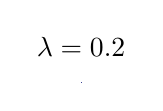
\begin{tikzpicture}[%
font=\footnotesize
]

\begin{axis}[%
width=0.951\figwidth,
height=\figheight,
at={(0\figwidth,0\figheight)},
scale only axis,
xmin=0,
xmax=3,
tick align=outside,
xlabel={Moneyness},
xmajorgrids,
ymin=0,
ymax=5,
ylabel={Remaining Time},
ymajorgrids,
zmin=0,
zmax=0.2,
zlabel={Relative Increase},
zmajorgrids,
view={50}{40},
axis background/.style={fill=white},
title style={font=\bfseries},
title={$\lambda = 0.2$},
axis x line*=bottom,
axis y line*=left,
axis z line*=left
]

\addplot3[%
surf,
shader=flat corner,draw=black,z buffer=sort,colormap={mymap}{[1pt] rgb(0pt)=(0.2081,0.1663,0.5292); rgb(1pt)=(0.211624,0.189781,0.577676); rgb(2pt)=(0.212252,0.213771,0.626971); rgb(3pt)=(0.2081,0.2386,0.677086); rgb(4pt)=(0.195905,0.264457,0.7279); rgb(5pt)=(0.170729,0.291938,0.779248); rgb(6pt)=(0.125271,0.324243,0.830271); rgb(7pt)=(0.0591333,0.359833,0.868333); rgb(8pt)=(0.0116952,0.38751,0.881957); rgb(9pt)=(0.00595714,0.408614,0.882843); rgb(10pt)=(0.0165143,0.4266,0.878633); rgb(11pt)=(0.0328524,0.443043,0.871957); rgb(12pt)=(0.0498143,0.458571,0.864057); rgb(13pt)=(0.0629333,0.47369,0.855438); rgb(14pt)=(0.0722667,0.488667,0.8467); rgb(15pt)=(0.0779429,0.503986,0.838371); rgb(16pt)=(0.0793476,0.520024,0.831181); rgb(17pt)=(0.0749429,0.537543,0.826271); rgb(18pt)=(0.0640571,0.556986,0.823957); rgb(19pt)=(0.0487714,0.577224,0.822829); rgb(20pt)=(0.0343429,0.596581,0.819852); rgb(21pt)=(0.0265,0.6137,0.8135); rgb(22pt)=(0.0238905,0.628662,0.803762); rgb(23pt)=(0.0230905,0.641786,0.791267); rgb(24pt)=(0.0227714,0.653486,0.776757); rgb(25pt)=(0.0266619,0.664195,0.760719); rgb(26pt)=(0.0383714,0.674271,0.743552); rgb(27pt)=(0.0589714,0.683757,0.725386); rgb(28pt)=(0.0843,0.692833,0.706167); rgb(29pt)=(0.113295,0.7015,0.685857); rgb(30pt)=(0.145271,0.709757,0.664629); rgb(31pt)=(0.180133,0.717657,0.642433); rgb(32pt)=(0.217829,0.725043,0.619262); rgb(33pt)=(0.258643,0.731714,0.595429); rgb(34pt)=(0.302171,0.737605,0.571186); rgb(35pt)=(0.348167,0.742433,0.547267); rgb(36pt)=(0.395257,0.7459,0.524443); rgb(37pt)=(0.44201,0.748081,0.503314); rgb(38pt)=(0.487124,0.749062,0.483976); rgb(39pt)=(0.530029,0.749114,0.466114); rgb(40pt)=(0.570857,0.748519,0.44939); rgb(41pt)=(0.609852,0.747314,0.433686); rgb(42pt)=(0.6473,0.7456,0.4188); rgb(43pt)=(0.683419,0.743476,0.404433); rgb(44pt)=(0.71841,0.741133,0.390476); rgb(45pt)=(0.752486,0.7384,0.376814); rgb(46pt)=(0.785843,0.735567,0.363271); rgb(47pt)=(0.818505,0.732733,0.34979); rgb(48pt)=(0.850657,0.7299,0.336029); rgb(49pt)=(0.882433,0.727433,0.3217); rgb(50pt)=(0.913933,0.725786,0.306276); rgb(51pt)=(0.944957,0.726114,0.288643); rgb(52pt)=(0.973895,0.731395,0.266648); rgb(53pt)=(0.993771,0.745457,0.240348); rgb(54pt)=(0.999043,0.765314,0.216414); rgb(55pt)=(0.995533,0.786057,0.196652); rgb(56pt)=(0.988,0.8066,0.179367); rgb(57pt)=(0.978857,0.827143,0.163314); rgb(58pt)=(0.9697,0.848138,0.147452); rgb(59pt)=(0.962586,0.870514,0.1309); rgb(60pt)=(0.958871,0.8949,0.113243); rgb(61pt)=(0.959824,0.921833,0.0948381); rgb(62pt)=(0.9661,0.951443,0.0755333); rgb(63pt)=(0.9763,0.9831,0.0538)},mesh/rows=25]
table[row sep=crcr, point meta=\thisrow{c}] {%
%
x	y	z	c\\
0	0.01	0.0198808226371358	0.0198808226371358\\
0	0.111836734693878	0.0643016281335618	0.0643016281335618\\
0	0.213673469387755	0.0860383410745243	0.0860383410745243\\
0	0.315510204081633	0.101296357715701	0.101296357715701\\
0	0.41734693877551	0.112974671832818	0.112974671832818\\
0	0.519183673469388	0.122293854757849	0.122293854757849\\
0	0.621020408163265	0.129917064612526	0.129917064612526\\
0	0.722857142857143	0.136256493012842	0.136256493012842\\
0	0.82469387755102	0.141590658570374	0.141590658570374\\
0	0.926530612244898	0.146118706324996	0.146118706324996\\
0	1.02836734693878	0.149988911676216	0.149988911676216\\
0	1.13020408163265	0.153315055510927	0.153315055510927\\
0	1.23204081632653	0.156186494973507	0.156186494973507\\
0	1.33387755102041	0.158674696470737	0.158674696470737\\
0	1.43571428571429	0.160837659282215	0.160837659282215\\
0	1.53755102040816	0.162723017867829	0.162723017867829\\
0	1.63938775510204	0.164370281957555	0.164370281957555\\
0	1.74122448979592	0.165812494260262	0.165812494260262\\
0	1.8430612244898	0.167077483054594	0.167077483054594\\
0	1.94489795918367	0.168188825726981	0.168188825726981\\
0	2.04673469387755	0.169166601469466	0.169166601469466\\
0	2.14857142857143	0.170027987187134	0.170027987187134\\
0	2.25040816326531	0.170787734811868	0.170787734811868\\
0	2.35224489795918	0.171458557553487	0.171458557553487\\
0	2.45408163265306	0.172051445289827	0.172051445289827\\
0	2.55591836734694	0.172575924154181	0.172575924154181\\
0	2.65775510204082	0.173040271708693	0.173040271708693\\
0	2.75959183673469	0.173451696430838	0.173451696430838\\
0	2.86142857142857	0.173816488275144	0.173816488275144\\
0	2.96326530612245	0.174140145612432	0.174140145612432\\
0	3.06510204081633	0.174427482738428	0.174427482738428\\
0	3.1669387755102	0.174682721301016	0.174682721301016\\
0	3.26877551020408	0.174909568340586	0.174909568340586\\
0	3.37061224489796	0.175111283127017	0.175111283127017\\
0	3.47244897959184	0.175290734578239	0.175290734578239\\
0	3.57428571428571	0.175450450725277	0.175450450725277\\
0	3.67612244897959	0.175592661434134	0.175592661434134\\
0	3.77795918367347	0.175719335389942	0.175719335389942\\
0	3.87979591836735	0.175832212183932	0.175832212183932\\
0	3.98163265306122	0.175932830205331	0.175932830205331\\
0	4.0834693877551	0.176022550932436	0.176022550932436\\
0	4.18530612244898	0.176102580121686	0.176102580121686\\
0	4.28714285714286	0.176173986321789	0.176173986321789\\
0	4.38897959183674	0.176237717072245	0.176237717072245\\
0	4.49081632653061	0.176294613095465	0.176294613095465\\
0	4.59265306122449	0.176345420748013	0.176345420748013\\
0	4.69448979591837	0.176390802954952	0.176390802954952\\
0	4.79632653061224	0.176431348823994	0.176431348823994\\
0	4.89816326530612	0.176467582107916	0.176467582107916\\
0	5	0.176499968658657	0.176499968658657\\
0.125	0.01	9.93766614385894e-05	9.93766614385894e-05\\
0.125	0.111836734693878	0.0206559551689525	0.0206559551689525\\
0.125	0.213673469387755	0.0384074151160625	0.0384074151160625\\
0.125	0.315510204081633	0.0519311224151515	0.0519311224151515\\
0.125	0.41734693877551	0.0626438831294785	0.0626438831294785\\
0.125	0.519183673469388	0.0713569680286243	0.0713569680286243\\
0.125	0.621020408163265	0.0785713987529336	0.0785713987529336\\
0.125	0.722857142857143	0.0846215865075946	0.0846215865075946\\
0.125	0.82469387755102	0.0897439414356159	0.0897439414356159\\
0.125	0.926530612244898	0.0941128205765335	0.0941128205765335\\
0.125	1.02836734693878	0.0978609813652928	0.0978609813652928\\
0.125	1.13020408163265	0.101092021486781	0.101092021486781\\
0.125	1.23204081632653	0.10388836251799	0.10388836251799\\
0.125	1.33387755102041	0.106316603046981	0.106316603046981\\
0.125	1.43571428571429	0.108431240122648	0.108431240122648\\
0.125	1.53755102040816	0.110277335670967	0.110277335670967\\
0.125	1.63938775510204	0.111892476257103	0.111892476257103\\
0.125	1.74122448979592	0.113308245021931	0.113308245021931\\
0.125	1.8430612244898	0.114551347949179	0.114551347949179\\
0.125	1.94489795918367	0.115644489561854	0.115644489561854\\
0.125	2.04673469387755	0.116607063374881	0.116607063374881\\
0.125	2.14857142857143	0.117455702707333	0.117455702707333\\
0.125	2.25040816326531	0.118204725257585	0.118204725257585\\
0.125	2.35224489795918	0.118866470795807	0.118866470795807\\
0.125	2.45408163265306	0.119451718255469	0.119451718255469\\
0.125	2.55591836734694	0.119969691361533	0.119969691361533\\
0.125	2.65775510204082	0.120428502892962	0.120428502892962\\
0.125	2.75959183673469	0.120835206041318	0.120835206041318\\
0.125	2.86142857142857	0.12119596216623	0.12119596216623\\
0.125	2.96326530612245	0.121516163625712	0.121516163625712\\
0.125	3.06510204081633	0.121800535865776	0.121800535865776\\
0.125	3.1669387755102	0.122053226440082	0.122053226440082\\
0.125	3.26877551020408	0.12227788027453	0.12227788027453\\
0.125	3.37061224489796	0.122477704414216	0.122477704414216\\
0.125	3.47244897959184	0.12265552374701	0.12265552374701\\
0.125	3.57428571428571	0.122813829087757	0.122813829087757\\
0.125	3.67612244897959	0.122954818770582	0.122954818770582\\
0.125	3.77795918367347	0.12308043470551	0.12308043470551\\
0.125	3.87979591836735	0.123192393699879	0.123192393699879\\
0.125	3.98163265306122	0.12329221471752	0.12329221471752\\
0.125	4.0834693877551	0.123381242643724	0.123381242643724\\
0.125	4.18530612244898	0.123460669037166	0.123460669037166\\
0.125	4.28714285714286	0.123531550277791	0.123531550277791\\
0.125	4.38897959183674	0.123594823459347	0.123594823459347\\
0.125	4.49081632653061	0.123651320324792	0.123651320324792\\
0.125	4.59265306122449	0.123701779500216	0.123701779500216\\
0.125	4.69448979591837	0.123746857247074	0.123746857247074\\
0.125	4.79632653061224	0.123787136467021	0.123787136467021\\
0.125	4.89816326530612	0.123823137308139	0.123823137308139\\
0.125	5	0.123855319958132	0.123855319958132\\
0.25	0.01	2.64817032709127e-09	2.64817032709127e-09\\
0.25	0.111836734693878	0.00457153705078958	0.00457153705078958\\
0.25	0.213673469387755	0.0143224014311132	0.0143224014311132\\
0.25	0.315510204081633	0.0237492698026274	0.0237492698026274\\
0.25	0.41734693877551	0.0320209061778352	0.0320209061778352\\
0.25	0.519183673469388	0.0391428904940248	0.0391428904940248\\
0.25	0.621020408163265	0.0452581623912486	0.0452581623912486\\
0.25	0.722857142857143	0.0505175600618624	0.0505175600618624\\
0.25	0.82469387755102	0.0550536889084289	0.0550536889084289\\
0.25	0.926530612244898	0.0589778867309349	0.0589778867309349\\
0.25	1.02836734693878	0.0623825427948636	0.0623825427948636\\
0.25	1.13020408163265	0.0653442897746835	0.0653442897746835\\
0.25	1.23204081632653	0.0679269226883102	0.0679269226883102\\
0.25	1.33387755102041	0.070183815777447	0.070183815777447\\
0.25	1.43571428571429	0.0721598606804366	0.0721598606804366\\
0.25	1.53755102040816	0.0738930071158544	0.0738930071158544\\
0.25	1.63938775510204	0.0754154884312959	0.0754154884312959\\
0.25	1.74122448979592	0.0767548011375475	0.0767548011375475\\
0.25	1.8430612244898	0.0779344928812873	0.0779344928812873\\
0.25	1.94489795918367	0.078974800892269	0.078974800892269\\
0.25	2.04673469387755	0.0798931726106456	0.0798931726106456\\
0.25	2.14857142857143	0.0807046935675032	0.0807046935675032\\
0.25	2.25040816326531	0.0814224409422281	0.0814224409422281\\
0.25	2.35224489795918	0.0820577775637736	0.0820577775637736\\
0.25	2.45408163265306	0.0826205977002369	0.0826205977002369\\
0.25	2.55591836734694	0.0831195335708195	0.0831195335708195\\
0.25	2.65775510204082	0.0835621298053684	0.0835621298053684\\
0.25	2.75959183673469	0.0839549904167806	0.0839549904167806\\
0.25	2.86142857142857	0.0843039060382085	0.0843039060382085\\
0.25	2.96326530612245	0.0846139597168246	0.0846139597168246\\
0.25	3.06510204081633	0.0848896196156037	0.0848896196156037\\
0.25	3.1669387755102	0.0851348178407981	0.0851348178407981\\
0.25	3.26877551020408	0.0853530184782395	0.0853530184782395\\
0.25	3.37061224489796	0.0855472763476363	0.0855472763476363\\
0.25	3.47244897959184	0.0857202878575854	0.0857202878575854\\
0.25	3.57428571428571	0.0858744351164722	0.0858744351164722\\
0.25	3.67612244897959	0.0860118242684247	0.0860118242684247\\
0.25	3.77795918367347	0.0861343188706427	0.0861343188706427\\
0.25	3.87979591836735	0.0862435690022049	0.0862435690022049\\
0.25	3.98163265306122	0.0863410366897496	0.0863410366897496\\
0.25	4.0834693877551	0.0864280181481896	0.0864280181481896\\
0.25	4.18530612244898	0.0865056632616381	0.0865056632616381\\
0.25	4.28714285714286	0.086574992668439	0.086574992668439\\
0.25	4.38897959183674	0.0866369127625461	0.0866369127625461\\
0.25	4.49081632653061	0.0866922288798236	0.0866922288798236\\
0.25	4.59265306122449	0.0867416569007929	0.0867416569007929\\
0.25	4.69448979591837	0.0867858334698392	0.0867858334698392\\
0.25	4.79632653061224	0.0868253239982276	0.0868253239982276\\
0.25	4.89816326530612	0.0868606356414621	0.0868606356414621\\
0.25	5	0.0868922142601879	0.0868922142601879\\
0.375	0.01	2.03776297743241e-16	2.03776297743241e-16\\
0.375	0.111836734693878	0.000660587723543788	0.000660587723543788\\
0.375	0.213673469387755	0.00435099021358512	0.00435099021358512\\
0.375	0.315510204081633	0.00953582119959086	0.00953582119959086\\
0.375	0.41734693877551	0.0149163858390065	0.0149163858390065\\
0.375	0.519183673469388	0.0200074087967396	0.0200074087967396\\
0.375	0.621020408163265	0.0246508754114831	0.0246508754114831\\
0.375	0.722857142857143	0.0288155806946354	0.0288155806946354\\
0.375	0.82469387755102	0.0325201027517757	0.0325201027517757\\
0.375	0.926530612244898	0.0358015458468327	0.0358015458468327\\
0.375	1.02836734693878	0.0387022696127867	0.0387022696127867\\
0.375	1.13020408163265	0.0412641728268968	0.0412641728268968\\
0.375	1.23204081632653	0.0435263192167163	0.0435263192167163\\
0.375	1.33387755102041	0.0455240908357585	0.0455240908357585\\
0.375	1.43571428571429	0.0472890462933625	0.0472890462933625\\
0.375	1.53755102040816	0.0488490964514878	0.0488490964514878\\
0.375	1.63938775510204	0.0502288108192168	0.0502288108192168\\
0.375	1.74122448979592	0.0514497639455418	0.0514497639455418\\
0.375	1.8430612244898	0.0525308784441844	0.0525308784441844\\
0.375	1.94489795918367	0.0534887450335941	0.0534887450335941\\
0.375	2.04673469387755	0.0543379119670623	0.0543379119670623\\
0.375	2.14857142857143	0.0550911422245941	0.0550911422245941\\
0.375	2.25040816326531	0.0557596397324678	0.0557596397324678\\
0.375	2.35224489795918	0.0563532471556561	0.0563532471556561\\
0.375	2.45408163265306	0.056880618251588	0.056880618251588\\
0.375	2.55591836734694	0.0573493677943196	0.0573493677943196\\
0.375	2.65775510204082	0.057766201896473	0.057766201896473\\
0.375	2.75959183673469	0.0581370312895416	0.0581370312895416\\
0.375	2.86142857142857	0.0584670698327121	0.0584670698327121\\
0.375	2.96326530612245	0.0587609202372177	0.0587609202372177\\
0.375	3.06510204081633	0.0590226487318867	0.0590226487318867\\
0.375	3.1669387755102	0.0592558501615731	0.0592558501615731\\
0.375	3.26877551020408	0.0594637048044835	0.0594637048044835\\
0.375	3.37061224489796	0.0596490280156412	0.0596490280156412\\
0.375	3.47244897959184	0.0598143136494312	0.0598143136494312\\
0.375	3.57428571428571	0.0599617720815449	0.0599617720815449\\
0.375	3.67612244897959	0.0600933635369249	0.0600933635369249\\
0.375	3.77795918367347	0.0602108273329261	0.0602108273329261\\
0.375	3.87979591836735	0.0603157075190727	0.0603157075190727\\
0.375	3.98163265306122	0.0604093756401523	0.0604093756401523\\
0.375	4.0834693877551	0.0604930503268147	0.0604930503268147\\
0.375	4.18530612244898	0.0605678149761801	0.0605678149761801\\
0.375	4.28714285714286	0.0606346331296629	0.0606346331296629\\
0.375	4.38897959183674	0.0606943620772981	0.0606943620772981\\
0.375	4.49081632653061	0.0607477648672287	0.0607477648672287\\
0.375	4.59265306122449	0.0607955209149206	0.0607955209149206\\
0.375	4.69448979591837	0.0608382353817762	0.0608382353817762\\
0.375	4.79632653061224	0.0608764474712895	0.0608764474712895\\
0.375	4.89816326530612	0.060910637772231	0.060910637772231\\
0.375	5	0.0609412347621751	0.0609412347621751\\
0.5	0.01	3.70078647069448e-26	3.70078647069448e-26\\
0.5	0.111836734693878	6.00414968802726e-05	6.00414968802726e-05\\
0.5	0.213673469387755	0.00105598376947452	0.00105598376947452\\
0.5	0.315510204081633	0.00331804807926943	0.00331804807926943\\
0.5	0.41734693877551	0.00627085425851384	0.00627085425851384\\
0.5	0.519183673469388	0.00945517399523579	0.00945517399523579\\
0.5	0.621020408163265	0.0126144468396184	0.0126144468396184\\
0.5	0.722857142857143	0.0156189184101276	0.0156189184101276\\
0.5	0.82469387755102	0.0184091546739231	0.0184091546739231\\
0.5	0.926530612244898	0.0209638011158372	0.0209638011158372\\
0.5	1.02836734693878	0.023281887939815	0.023281887939815\\
0.5	1.13020408163265	0.0253730841314174	0.0253730841314174\\
0.5	1.23204081632653	0.0272522705984497	0.0272522705984497\\
0.5	1.33387755102041	0.0289364964566318	0.0289364964566318\\
0.5	1.43571428571429	0.0304432758239252	0.0304432758239252\\
0.5	1.53755102040816	0.0317896517880856	0.0317896517880856\\
0.5	1.63938775510204	0.0329917050624156	0.0329917050624156\\
0.5	1.74122448979592	0.0340643220820368	0.0340643220820368\\
0.5	1.8430612244898	0.0350211141875702	0.0350211141875702\\
0.5	1.94489795918367	0.0358744236038149	0.0358744236038149\\
0.5	2.04673469387755	0.0366353776802226	0.0366353776802226\\
0.5	2.14857142857143	0.0373139681837943	0.0373139681837943\\
0.5	2.25040816326531	0.0379191416839826	0.0379191416839826\\
0.5	2.35224489795918	0.0384588927153609	0.0384588927153609\\
0.5	2.45408163265306	0.0389403548781813	0.0389403548781813\\
0.5	2.55591836734694	0.0393698871835446	0.0393698871835446\\
0.5	2.65775510204082	0.0397531542752253	0.0397531542752253\\
0.5	2.75959183673469	0.0400951999727955	0.0400951999727955\\
0.5	2.86142857142857	0.0404005140710732	0.0404005140710732\\
0.5	2.96326530612245	0.0406730926180999	0.0406730926180999\\
0.5	3.06510204081633	0.0409164920528677	0.0409164920528677\\
0.5	3.1669387755102	0.0411338776625956	0.0411338776625956\\
0.5	3.26877551020408	0.0413280668479797	0.0413280668479797\\
0.5	3.37061224489796	0.0415015676830869	0.0415015676830869\\
0.5	3.47244897959184	0.0416566132369759	0.0416566132369759\\
0.5	3.57428571428571	0.041795192094747	0.041795192094747\\
0.5	3.67612244897959	0.0419190754816385	0.0419190754816385\\
0.5	3.77795918367347	0.0420298413582111	0.0420298413582111\\
0.5	3.87979591836735	0.0421288958195303	0.0421288958195303\\
0.5	3.98163265306122	0.0422174920977234	0.0422174920977234\\
0.5	4.0834693877551	0.042296747435981	0.042296747435981\\
0.5	4.18530612244898	0.0423676580732731	0.0423676580732731\\
0.5	4.28714285714286	0.0424311125528428	0.0424311125528428\\
0.5	4.38897959183674	0.0424879035438755	0.0424879035438755\\
0.5	4.49081632653061	0.0425387383444905	0.0425387383444905\\
0.5	4.59265306122449	0.0425842482152004	0.0425842482152004\\
0.5	4.69448979591837	0.0426249966750476	0.0426249966750476\\
0.5	4.79632653061224	0.0426614868775635	0.0426614868775635\\
0.5	4.89816326530612	0.0426941681794362	0.0426941681794362\\
0.5	5	0.0427234419403345	0.0427234419403345\\
0.625	0.01	1.46000670492715e-38	1.46000670492715e-38\\
0.625	0.111836734693878	3.34669946288913e-06	3.34669946288913e-06\\
0.625	0.213673469387755	0.000201748383351537	0.000201748383351537\\
0.625	0.315510204081633	0.000990134180091808	0.000990134180091808\\
0.625	0.41734693877551	0.00235998317967082	0.00235998317967082\\
0.625	0.519183673469388	0.00410403500655054	0.00410403500655054\\
0.625	0.621020408163265	0.00603066048013561	0.00603066048013561\\
0.625	0.722857142857143	0.00800564454852661	0.00800564454852661\\
0.625	0.82469387755102	0.00994409625916895	0.00994409625916895\\
0.625	0.926530612244898	0.0117958149037926	0.0117958149037926\\
0.625	1.02836734693878	0.0135334563343116	0.0135334563343116\\
0.625	1.13020408163265	0.015144307906199	0.015144307906199\\
0.625	1.23204081632653	0.0166248410310474	0.0166248410310474\\
0.625	1.33387755102041	0.0179771631757387	0.0179771631757387\\
0.625	1.43571428571429	0.0192067204095036	0.0192067204095036\\
0.625	1.53755102040816	0.0203208142606873	0.0203208142606873\\
0.625	1.63938775510204	0.021327648501819	0.021327648501819\\
0.625	1.74122448979592	0.0222357219036005	0.0222357219036005\\
0.625	1.8430612244898	0.0230534477410352	0.0230534477410352\\
0.625	1.94489795918367	0.0237889223425405	0.0237889223425405\\
0.625	2.04673469387755	0.0244497916665887	0.0244497916665887\\
0.625	2.14857142857143	0.0250431821772795	0.0250431821772795\\
0.625	2.25040816326531	0.0255756735810331	0.0255756735810331\\
0.625	2.35224489795918	0.0260532984266958	0.0260532984266958\\
0.625	2.45408163265306	0.0264815585158764	0.0264815585158764\\
0.625	2.55591836734694	0.0268654513818812	0.0268654513818812\\
0.625	2.65775510204082	0.0272095023283437	0.0272095023283437\\
0.625	2.75959183673469	0.0275177990321719	0.0275177990321719\\
0.625	2.86142857142857	0.0277940267454274	0.0277940267454274\\
0.625	2.96326530612245	0.0280415028331983	0.0280415028331983\\
0.625	3.06510204081633	0.0282632098636039	0.0282632098636039\\
0.625	3.1669387755102	0.0284618267919793	0.0284618267919793\\
0.625	3.26877551020408	0.0286397580016897	0.0286397580016897\\
0.625	3.37061224489796	0.0287991601115426	0.0287991601115426\\
0.625	3.47244897959184	0.0289419665568316	0.0289419665568316\\
0.625	3.57428571428571	0.029069910013216	0.029069910013216\\
0.625	3.67612244897959	0.0291845427707069	0.0291845427707069\\
0.625	3.77795918367347	0.029287255186556	0.029287255186556\\
0.625	3.87979591836735	0.0293792923560839	0.0293792923560839\\
0.625	3.98163265306122	0.0294617691431654	0.0294617691431654\\
0.625	4.0834693877551	0.029535683709775	0.029535683709775\\
0.625	4.18530612244898	0.0296019296785205	0.0296019296785205\\
0.625	4.28714285714286	0.0296613070547041	0.0296613070547041\\
0.625	4.38897959183674	0.0297145320260241	0.0297145320260241\\
0.625	4.49081632653061	0.0297622457491673	0.0297622457491673\\
0.625	4.59265306122449	0.0298050222236403	0.0298050222236403\\
0.625	4.69448979591837	0.0298433753445068	0.0298433753445068\\
0.625	4.79632653061224	0.0298777652174151	0.0298777652174151\\
0.625	4.89816326530612	0.0299086038115028	0.0299086038115028\\
0.625	5	0.0299362600185089	0.0299362600185089\\
0.75	0.01	1.20104644349094e-53	1.20104644349094e-53\\
0.75	0.111836734693878	1.12436305019756e-07	1.12436305019756e-07\\
0.75	0.213673469387755	3.00080863122672e-05	3.00080863122672e-05\\
0.75	0.315510204081633	0.000251317370241044	0.000251317370241044\\
0.75	0.41734693877551	0.00078985404167758	0.00078985404167758\\
0.75	0.519183673469388	0.00162708342800575	0.00162708342800575\\
0.75	0.621020408163265	0.00268064747594418	0.00268064747594418\\
0.75	0.722857142857143	0.00386387523166428	0.00386387523166428\\
0.75	0.82469387755102	0.00510618440347022	0.00510618440347022\\
0.75	0.926530612244898	0.00635595782951644	0.00635595782951644\\
0.75	1.02836734693878	0.00757781244708229	0.00757781244708229\\
0.75	1.13020408163265	0.00874881972079334	0.00874881972079334\\
0.75	1.23204081632653	0.00985512672837668	0.00985512672837668\\
0.75	1.33387755102041	0.0108892984314953	0.0108892984314953\\
0.75	1.43571428571429	0.0118483377167939	0.0118483377167939\\
0.75	1.53755102040816	0.0127322494613304	0.0127322494613304\\
0.75	1.63938775510204	0.0135430146335706	0.0135430146335706\\
0.75	1.74122448979592	0.0142838645450633	0.0142838645450633\\
0.75	1.8430612244898	0.0149587716867943	0.0149587716867943\\
0.75	1.94489795918367	0.015572095729664	0.015572095729664\\
0.75	2.04673469387755	0.0161283402678761	0.0161283402678761\\
0.75	2.14857142857143	0.0166319884123104	0.0166319884123104\\
0.75	2.25040816326531	0.0170873943982736	0.0170873943982736\\
0.75	2.35224489795918	0.0174987148634354	0.0174987148634354\\
0.75	2.45408163265306	0.0178698680898787	0.0178698680898787\\
0.75	2.55591836734694	0.0182045128180852	0.0182045128180852\\
0.75	2.65775510204082	0.0185060406123008	0.0185060406123008\\
0.75	2.75959183673469	0.0187775774581405	0.0187775774581405\\
0.75	2.86142857142857	0.0190219914972063	0.0190219914972063\\
0.75	2.96326530612245	0.0192419046862121	0.0192419046862121\\
0.75	3.06510204081633	0.0194397068061824	0.0194397068061824\\
0.75	3.1669387755102	0.0196175707093029	0.0196175707093029\\
0.75	3.26877551020408	0.0197774680258207	0.0197774680258207\\
0.75	3.37061224489796	0.0199211847960373	0.0199211847960373\\
0.75	3.47244897959184	0.0200503366680457	0.0200503366680457\\
0.75	3.57428571428571	0.0201663834286177	0.0201663834286177\\
0.75	3.67612244897959	0.0202706427257006	0.0202706427257006\\
0.75	3.77795918367347	0.0203643029059373	0.0203643029059373\\
0.75	3.87979591836735	0.0204484349364593	0.0204484349364593\\
0.75	3.98163265306122	0.0205240034120702	0.0205240034120702\\
0.75	4.0834693877551	0.0205918766705856	0.0205918766705856\\
0.75	4.18530612244898	0.0206528360533163	0.0206528360533163\\
0.75	4.28714285714286	0.0207075843565079	0.0207075843565079\\
0.75	4.38897959183674	0.0207567535244987	0.0207567535244987\\
0.75	4.49081632653061	0.0208009116375458	0.0208009116375458\\
0.75	4.59265306122449	0.0208405692475123	0.0208405692475123\\
0.75	4.69448979591837	0.0208761851135189	0.0208761851135189\\
0.75	4.79632653061224	0.0209081713876825	0.0209081713876825\\
0.75	4.89816326530612	0.02093689829852	0.02093689829852\\
0.75	5	0.0209626983767164	0.0209626983767164\\
0.875	0.01	2.01344381665123e-71	2.01344381665123e-71\\
0.875	0.111836734693878	2.24953548041261e-09	2.24953548041261e-09\\
0.875	0.213673469387755	3.44612683953096e-06	3.44612683953096e-06\\
0.875	0.315510204081633	5.39098619468298e-05	5.39098619468298e-05\\
0.875	0.41734693877551	0.0002338442109669	0.0002338442109669\\
0.875	0.519183673469388	0.000586511539040859	0.000586511539040859\\
0.875	0.621020408163265	0.00110341090148634	0.00110341090148634\\
0.875	0.722857142857143	0.00174966167439324	0.00174966167439324\\
0.875	0.82469387755102	0.00248423089923642	0.00248423089923642\\
0.875	0.926530612244898	0.00326972139220079	0.00326972139220079\\
0.875	1.02836734693878	0.00407572018582725	0.00407572018582725\\
0.875	1.13020408163265	0.00487910729546832	0.00487910729546832\\
0.875	1.23204081632653	0.00566317748496375	0.00566317748496375\\
0.875	1.33387755102041	0.00641644068791323	0.00641644068791323\\
0.875	1.43571428571429	0.00713146235435403	0.00713146235435403\\
0.875	1.53755102040816	0.00780387007769964	0.00780387007769964\\
0.875	1.63938775510204	0.00843155087836511	0.00843155087836511\\
0.875	1.74122448979592	0.0090140234596237	0.0090140234596237\\
0.875	1.8430612244898	0.00955195727083582	0.00955195727083582\\
0.875	1.94489795918367	0.0100468092946727	0.0100468092946727\\
0.875	2.04673469387755	0.0105005528533223	0.0105005528533223\\
0.875	2.14857142857143	0.0109154772319249	0.0109154772319249\\
0.875	2.25040816326531	0.011294041254695	0.011294041254695\\
0.875	2.35224489795918	0.0116387676735304	0.0116387676735304\\
0.875	2.45408163265306	0.0119521682562696	0.0119521682562696\\
0.875	2.55591836734694	0.0122366918505298	0.0122366918505298\\
0.875	2.65775510204082	0.0124946895519718	0.0124946895519718\\
0.875	2.75959183673469	0.012728392528705	0.012728392528705\\
0.875	2.86142857142857	0.0129398991396959	0.0129398991396959\\
0.875	2.96326530612245	0.013131168811338	0.013131168811338\\
0.875	3.06510204081633	0.0133040207637556	0.0133040207637556\\
0.875	3.1669387755102	0.0134601361543556	0.0134601361543556\\
0.875	3.26877551020408	0.0136010625669865	0.0136010625669865\\
0.875	3.37061224489796	0.0137282200485594	0.0137282200485594\\
0.875	3.47244897959184	0.0138429081021896	0.0138429081021896\\
0.875	3.57428571428571	0.0139463132027914	0.0139463132027914\\
0.875	3.67612244897959	0.0140395165197066	0.0140395165197066\\
0.875	3.77795918367347	0.0141235016205193	0.0141235016205193\\
0.875	3.87979591836735	0.0141991619976762	0.0141991619976762\\
0.875	3.98163265306122	0.0142673083101611	0.0142673083101611\\
0.875	4.0834693877551	0.0143286752702834	0.0143286752702834\\
0.875	4.18530612244898	0.0143839281337038	0.0143839281337038\\
0.875	4.28714285714286	0.0144336687714511	0.0144336687714511\\
0.875	4.38897959183674	0.0144784413176823	0.0144784413176823\\
0.875	4.49081632653061	0.0145187373976574	0.0145187373976574\\
0.875	4.59265306122449	0.0145550009478847	0.0145550009478847\\
0.875	4.69448979591837	0.0145876326454418	0.0145876326454418\\
0.875	4.79632653061224	0.0146169939667027	0.0146169939667027\\
0.875	4.89816326530612	0.0146434108975692	0.0146434108975692\\
0.875	5	0.0146671773181734	0.0146671773181734\\
1	0.01	6.78223653234785e-92	6.78223653234785e-92\\
1	0.111836734693878	2.65740084855957e-11	2.65740084855957e-11\\
1	0.213673469387755	3.03637859813333e-07	3.03637859813333e-07\\
1	0.315510204081633	9.72371074817936e-06	9.72371074817936e-06\\
1	0.41734693877551	6.09793675933003e-05	6.09793675933003e-05\\
1	0.519183673469388	0.00019150267717967	0.00019150267717967\\
1	0.621020408163265	0.000419168707682541	0.000419168707682541\\
1	0.722857142857143	0.000741053974835378	0.000741053974835378\\
1	0.82469387755102	0.00114186874177045	0.00114186874177045\\
1	0.926530612244898	0.00160165140973324	0.00160165140973324\\
1	1.02836734693878	0.00210046249685465	0.00210046249685465\\
1	1.13020408163265	0.00262066499248423	0.00262066499248423\\
1	1.23204081632653	0.00314773788732588	0.00314773788732588\\
1	1.33387755102041	0.00367031819241925	0.00367031819241925\\
1	1.43571428571429	0.0041798894811167	0.0041798894811167\\
1	1.53755102040816	0.00467034430044051	0.00467034430044051\\
1	1.63938775510204	0.00513753453331019	0.00513753453331019\\
1	1.74122448979592	0.0055788612528641	0.0055788612528641\\
1	1.8430612244898	0.00599292284774556	0.00599292284774556\\
1	1.94489795918367	0.00637922398530789	0.00637922398530789\\
1	2.04673469387755	0.00673794063666689	0.00673794063666689\\
1	2.14857142857143	0.00706973363497231	0.00706973363497231\\
1	2.25040816326531	0.00737560275476256	0.00737560275476256\\
1	2.35224489795918	0.00765677385407348	0.00765677385407348\\
1	2.45408163265306	0.00791461257564728	0.00791461257564728\\
1	2.55591836734694	0.0081505591431453	0.0081505591431453\\
1	2.65775510204082	0.00836607976650853	0.00836607976650853\\
1	2.75959183673469	0.00856263102931753	0.00856263102931753\\
1	2.86142857142857	0.00874163435594093	0.00874163435594093\\
1	2.96326530612245	0.00890445825380859	0.00890445825380859\\
1	3.06510204081633	0.00905240651112308	0.00905240651112308\\
1	3.1669387755102	0.00918671091986669	0.00918671091986669\\
1	3.26877551020408	0.00930852740460778	0.00930852740460778\\
1	3.37061224489796	0.00941893468407643	0.00941893468407643\\
1	3.47244897959184	0.00951893478728908	0.00951893478728908\\
1	3.57428571428571	0.00960945489953825	0.00960945489953825\\
1	3.67612244897959	0.00969135013428217	0.00969135013428217\\
1	3.77795918367347	0.00976540692168671	0.00976540692168671\\
1	3.87979591836735	0.00983234677873485	0.00983234677873485\\
1	3.98163265306122	0.00989283028376411	0.00989283028376411\\
1	4.0834693877551	0.00994746112345585	0.00994746112345585\\
1	4.18530612244898	0.0099967901154019	0.0099967901154019\\
1	4.28714285714286	0.0100413191365618	0.0100413191365618\\
1	4.38897959183674	0.0100815049088929	0.0100815049088929\\
1	4.49081632653061	0.0101177626095254	0.0101177626095254\\
1	4.59265306122449	0.0101504692851138	0.0101504692851138\\
1	4.69448979591837	0.0101799670592685	0.0101799670592685\\
1	4.79632653061224	0.0102065661288954	0.0102065661288954\\
1	4.89816326530612	0.01023054755038	0.01023054755038\\
1	5	0.0102521658202428	0.0102521658202428\\
1.125	0.01	4.54822824865968e-115	4.54822824865968e-115\\
1.125	0.111836734693878	1.84200693963409e-13	1.84200693963409e-13\\
1.125	0.213673469387755	2.04277294433038e-08	2.04277294433038e-08\\
1.125	0.315510204081633	1.46884959418657e-06	1.46884959418657e-06\\
1.125	0.41734693877551	1.39575631341316e-05	1.39575631341316e-05\\
1.125	0.519183673469388	5.6462492603842e-05	5.6462492603842e-05\\
1.125	0.621020408163265	0.000146544555888933	0.000146544555888933\\
1.125	0.722857142857143	0.000292805214388744	0.000292805214388744\\
1.125	0.82469387755102	0.000494666933346174	0.000494666933346174\\
1.125	0.926530612244898	0.000745348393936351	0.000745348393936351\\
1.125	1.02836734693878	0.00103498987496577	0.00103498987496577\\
1.125	1.13020408163265	0.00135291630014476	0.00135291630014476\\
1.125	1.23204081632653	0.00168899411896807	0.00168899411896807\\
1.125	1.33387755102041	0.00203431568119632	0.00203431568119632\\
1.125	1.43571428571429	0.00238145405454163	0.00238145405454163\\
1.125	1.53755102040816	0.00272447023489255	0.00272447023489255\\
1.125	1.63938775510204	0.00305879227059173	0.00305879227059173\\
1.125	1.74122448979592	0.0033810389757429	0.0033810389757429\\
1.125	1.8430612244898	0.00368882971627333	0.00368882971627333\\
1.125	1.94489795918367	0.00398060228907655	0.00398060228907655\\
1.125	2.04673469387755	0.00425544930912773	0.00425544930912773\\
1.125	2.14857142857143	0.00451297688390574	0.00451297688390574\\
1.125	2.25040816326531	0.00475318574910794	0.00475318574910794\\
1.125	2.35224489795918	0.00497637322913227	0.00497637322913227\\
1.125	2.45408163265306	0.00518305360778238	0.00518305360778238\\
1.125	2.55591836734694	0.00537389428905386	0.00537389428905386\\
1.125	2.65775510204082	0.00554966522235522	0.00554966522235522\\
1.125	2.75959183673469	0.00571119930325247	0.00571119930325247\\
1.125	2.86142857142857	0.0058593617507674	0.0058593617507674\\
1.125	2.96326530612245	0.00599502675720012	0.00599502675720012\\
1.125	3.06510204081633	0.00611905998203081	0.00611905998203081\\
1.125	3.1669387755102	0.00623230570697959	0.00623230570697959\\
1.125	3.26877551020408	0.00633557768164055	0.00633557768164055\\
1.125	3.37061224489796	0.00642965286913507	0.00642965286913507\\
1.125	3.47244897959184	0.00651526745175854	0.00651526745175854\\
1.125	3.57428571428571	0.00659311458119474	0.00659311458119474\\
1.125	3.67612244897959	0.00666384346022747	0.00666384346022747\\
1.125	3.77795918367347	0.00672805942646947	0.00672805942646947\\
1.125	3.87979591836735	0.00678632477657098	0.00678632477657098\\
1.125	3.98163265306122	0.00683916012437545	0.00683916012437545\\
1.125	4.0834693877551	0.00688704613086874	0.00688704613086874\\
1.125	4.18530612244898	0.00693042547945784	0.00693042547945784\\
1.125	4.28714285714286	0.00696970499873048	0.00696970499873048\\
1.125	4.38897959183674	0.00700525785771728	0.00700525785771728\\
1.125	4.49081632653061	0.00703742577689682	0.00703742577689682\\
1.125	4.59265306122449	0.00706652121264396	0.00706652121264396\\
1.125	4.69448979591837	0.00709282948425113	0.00709282948425113\\
1.125	4.79632653061224	0.00711661082164266	0.00711661082164266\\
1.125	4.89816326530612	0.00713810231893387	0.00713810231893387\\
1.125	5	0.00715751978444852	0.00715751978444852\\
1.25	0.01	6.03354000958525e-141	6.03354000958525e-141\\
1.25	0.111836734693878	7.45723969539844e-16	7.45723969539844e-16\\
1.25	0.213673469387755	1.04544583650273e-09	1.04544583650273e-09\\
1.25	0.315510204081633	1.85234666221095e-07	1.85234666221095e-07\\
1.25	0.41734693877551	2.79631063283471e-06	2.79631063283471e-06\\
1.25	0.519183673469388	1.49942713395933e-05	1.49942713395933e-05\\
1.25	0.621020408163265	4.70390772447756e-05	4.70390772447756e-05\\
1.25	0.722857142857143	0.00010769288345139	0.00010769288345139\\
1.25	0.82469387755102	0.000201549767925956	0.000201549767925956\\
1.25	0.926530612244898	0.00032887453075993	0.00032887453075993\\
1.25	1.02836734693878	0.000486689852709873	0.000486689852709873\\
1.25	1.13020408163265	0.000670096447233008	0.000670096447233008\\
1.25	1.23204081632653	0.000873370357914268	0.000873370357914268\\
1.25	1.33387755102041	0.00109072680709635	0.00109072680709635\\
1.25	1.43571428571429	0.0013167861161946	0.0013167861161946\\
1.25	1.53755102040816	0.001546817532767	0.001546817532767\\
1.25	1.63938775510204	0.00177683375460223	0.00177683375460223\\
1.25	1.74122448979592	0.00200359292601113	0.00200359292601113\\
1.25	1.8430612244898	0.0022245481478623	0.0022245481478623\\
1.25	1.94489795918367	0.00243777097266022	0.00243777097266022\\
1.25	2.04673469387755	0.00264186548084296	0.00264186548084296\\
1.25	2.14857142857143	0.00283588277688366	0.00283588277688366\\
1.25	2.25040816326531	0.00301924131229894	0.00301924131229894\\
1.25	2.35224489795918	0.00319165563919263	0.00319165563919263\\
1.25	2.45408163265306	0.00335307448937843	0.00335307448937843\\
1.25	2.55591836734694	0.00350362808082905	0.00350362808082905\\
1.25	2.65775510204082	0.00364358401566193	0.00364358401566193\\
1.25	2.75959183673469	0.00377331087935631	0.00377331087935631\\
1.25	2.86142857142857	0.0038932485667334	0.0038932485667334\\
1.25	2.96326530612245	0.00400388437422093	0.00400388437422093\\
1.25	3.06510204081633	0.00410573396462428	0.00410573396462428\\
1.25	3.1669387755102	0.00419932640204816	0.00419932640204816\\
1.25	3.26877551020408	0.00428519255399543	0.00428519255399543\\
1.25	3.37061224489796	0.00436385625539451	0.00436385625539451\\
1.25	3.47244897959184	0.00443582772022397	0.00443582772022397\\
1.25	3.57428571428571	0.00450159876810891	0.00450159876810891\\
1.25	3.67612244897959	0.00456163950499564	0.00456163950499564\\
1.25	3.77795918367347	0.00461639615894666	0.00461639615894666\\
1.25	3.87979591836735	0.00466628982491828	0.00466628982491828\\
1.25	3.98163265306122	0.00471171591700452	0.00471171591700452\\
1.25	4.0834693877551	0.00475304416404369	0.00475304416404369\\
1.25	4.18530612244898	0.00479061901566001	0.00479061901566001\\
1.25	4.28714285714286	0.00482476035165819	0.00482476035165819\\
1.25	4.38897959183674	0.00485576440901732	0.00485576440901732\\
1.25	4.49081632653061	0.00488390485826111	0.00488390485826111\\
1.25	4.59265306122449	0.00490943397533368	0.00490943397533368\\
1.25	4.69448979591837	0.00493258386681786	0.00493258386681786\\
1.25	4.79632653061224	0.00495356771584596	0.00495356771584596\\
1.25	4.89816326530612	0.00497258102375385	0.00497258102375385\\
1.25	5	0.00498980282873505	0.00498980282873505\\
1.375	0.01	1.5760399884267e-169	1.5760399884267e-169\\
1.375	0.111836734693878	1.75704516481191e-18	1.75704516481191e-18\\
1.375	0.213673469387755	4.05812771967413e-11	4.05812771967413e-11\\
1.375	0.315510204081633	1.94517001884367e-08	1.94517001884367e-08\\
1.375	0.41734693877551	4.89231292278707e-07	4.89231292278707e-07\\
1.375	0.519183673469388	3.57895693712135e-06	3.57895693712135e-06\\
1.375	0.621020408163265	1.3835776407832e-05	1.3835776407832e-05\\
1.375	0.722857142857143	3.68018842934355e-05	3.68018842934355e-05\\
1.375	0.82469387755102	7.7100825705536e-05	7.7100825705536e-05\\
1.375	0.926530612244898	0.000137356034065995	0.000137356034065995\\
1.375	1.02836734693878	0.000218051048624204	0.000218051048624204\\
1.375	1.13020408163265	0.000317928635140791	0.000317928635140791\\
1.375	1.23204081632653	0.000434560568586284	0.000434560568586284\\
1.375	1.33387755102041	0.000564881730289494	0.000564881730289494\\
1.375	1.43571428571429	0.000705608144984257	0.000705608144984257\\
1.375	1.53755102040816	0.000853527567836477	0.000853527567836477\\
1.375	1.63938775510204	0.00100568063424918	0.00100568063424918\\
1.375	1.74122448979592	0.00115945872729651	0.00115945872729651\\
1.375	1.8430612244898	0.00131264334659708	0.00131264334659708\\
1.375	1.94489795918367	0.00146340709257813	0.00146340709257813\\
1.375	2.04673469387755	0.00161029127516049	0.00161029127516049\\
1.375	2.14857142857143	0.00175217072829886	0.00175217072829886\\
1.375	2.25040816326531	0.00188821295114305	0.00188821295114305\\
1.375	2.35224489795918	0.00201783615054028	0.00201783615054028\\
1.375	2.45408163265306	0.00214066896290226	0.00214066896290226\\
1.375	2.55591836734694	0.00225651340728414	0.00225651340728414\\
1.375	2.65775510204082	0.00236531181063847	0.00236531181063847\\
1.375	2.75959183673469	0.00246711792828654	0.00246711792828654\\
1.375	2.86142857142857	0.00256207216631862	0.00256207216631862\\
1.375	2.96326530612245	0.00265038063193586	0.00265038063193586\\
1.375	3.06510204081633	0.00273229764619491	0.00273229764619491\\
1.375	3.1669387755102	0.00280811131907144	0.00280811131907144\\
1.375	3.26877551020408	0.00287813178735704	0.00287813178735704\\
1.375	3.37061224489796	0.00294268173702271	0.00294268173702271\\
1.375	3.47244897959184	0.0030020888637122	0.0030020888637122\\
1.375	3.57428571428571	0.00305667996179989	0.00305667996179989\\
1.375	3.67612244897959	0.00310677637011648	0.00310677637011648\\
1.375	3.77795918367347	0.00315269053871877	0.00315269053871877\\
1.375	3.87979591836735	0.00319472351469153	0.00319472351469153\\
1.375	3.98163265306122	0.00323316317531116	0.00323316317531116\\
1.375	4.0834693877551	0.0032682830637827	0.0032682830637827\\
1.375	4.18530612244898	0.00330034170624612	0.00330034170624612\\
1.375	4.28714285714286	0.00332958230904038	0.00332958230904038\\
1.375	4.38897959183674	0.00335623275259639	0.00335623275259639\\
1.375	4.49081632653061	0.00338050581311229	0.00338050581311229\\
1.375	4.59265306122449	0.00340259955565903	0.00340259955565903\\
1.375	4.69448979591837	0.00342269785286884	0.00342269785286884\\
1.375	4.79632653061224	0.00344097099214836	0.00344097099214836\\
1.375	4.89816326530612	0.00345757634167963	0.00345757634167963\\
1.375	5	0.00347265905154538	0.00347265905154538\\
1.5	0.01	8.07877061333241e-201	8.07877061333241e-201\\
1.5	0.111836734693878	2.40279005726969e-21	2.40279005726969e-21\\
1.5	0.213673469387755	1.19200551826941e-12	1.19200551826941e-12\\
1.5	0.315510204081633	1.69740082972054e-09	1.69740082972054e-09\\
1.5	0.41734693877551	7.4606726103739e-08	7.4606726103739e-08\\
1.5	0.519183673469388	7.6646851607057e-07	7.6646851607057e-07\\
1.5	0.621020408163265	3.72297006643067e-06	3.72297006643067e-06\\
1.5	0.722857142857143	1.16667117383771e-05	1.16667117383771e-05\\
1.5	0.82469387755102	2.76497729681324e-05	2.76497729681324e-05\\
1.5	0.926530612244898	5.42229846401895e-05	5.42229846401895e-05\\
1.5	1.02836734693878	9.29490386668139e-05	9.29490386668139e-05\\
1.5	1.13020408163265	0.000144296579040326	0.000144296579040326\\
1.5	1.23204081632653	0.000207781554158505	0.000207781554158505\\
1.5	1.33387755102041	0.000282214965915394	0.000282214965915394\\
1.5	1.43571428571429	0.00036596304259493	0.00036596304259493\\
1.5	1.53755102040816	0.000457172149277392	0.000457172149277392\\
1.5	1.63938775510204	0.000553941757990703	0.000553941757990703\\
1.5	1.74122448979592	0.000654445671287342	0.000654445671287342\\
1.5	1.8430612244898	0.000757009140933492	0.000757009140933492\\
1.5	1.94489795918367	0.000860151660621367	0.000860151660621367\\
1.5	2.04673469387755	0.000962604755176202	0.000962604755176202\\
1.5	2.14857142857143	0.00106331259933858	0.00106331259933858\\
1.5	2.25040816326531	0.00116142158151177	0.00116142158151177\\
1.5	2.35224489795918	0.00125626334770499	0.00125626334770499\\
1.5	2.45408163265306	0.00134733455045872	0.00134733455045872\\
1.5	2.55591836734694	0.00143427550505958	0.00143427550505958\\
1.5	2.65775510204082	0.00151684919021688	0.00151684919021688\\
1.5	2.75959183673469	0.00159492147616185	0.00159492147616185\\
1.5	2.86142857142857	0.00166844307310497	0.00166844307310497\\
1.5	2.96326530612245	0.00173743342636359	0.00173743342636359\\
1.5	3.06510204081633	0.00180196660817693	0.00180196660817693\\
1.5	3.1669387755102	0.00186215914459613	0.00186215914459613\\
1.5	3.26877551020408	0.00191815964955154	0.00191815964955154\\
1.5	3.37061224489796	0.00197014010302928	0.00197014010302928\\
1.5	3.47244897959184	0.00201828859594276	0.00201828859594276\\
1.5	3.57428571428571	0.00206280336343426	0.00206280336343426\\
1.5	3.67612244897959	0.00210388793585217	0.00210388793585217\\
1.5	3.77795918367347	0.00214174724897711	0.00214174724897711\\
1.5	3.87979591836735	0.00217658456982053	0.00217658456982053\\
1.5	3.98163265306122	0.00220859910990976	0.00220859910990976\\
1.5	4.0834693877551	0.00223798421339342	0.00223798421339342\\
1.5	4.18530612244898	0.00226492602193665	0.00226492602193665\\
1.5	4.28714285714286	0.00228960253188241	0.00228960253188241\\
1.5	4.38897959183674	0.00231218297137074	0.00231218297137074\\
1.5	4.49081632653061	0.00233282743598866	0.00233282743598866\\
1.5	4.59265306122449	0.00235168673109931	0.00235168673109931\\
1.5	4.69448979591837	0.00236890237734613	0.00236890237734613\\
1.5	4.79632653061224	0.00238460674304572	0.00238460674304572\\
1.5	4.89816326530612	0.00239892327338217	0.00239892327338217\\
1.5	5	0.00241196679160748	0.00241196679160748\\
1.625	0.01	8.10542666217349e-235	8.10542666217349e-235\\
1.625	0.111836734693878	1.90299788068978e-24	1.90299788068978e-24\\
1.625	0.213673469387755	2.64448991489449e-14	2.64448991489449e-14\\
1.625	0.315510204081633	1.22876167587069e-10	1.22876167587069e-10\\
1.625	0.41734693877551	9.90147619474651e-09	9.90147619474651e-09\\
1.625	0.519183673469388	1.47063606210524e-07	1.47063606210524e-07\\
1.625	0.621020408163265	9.1519945949821e-07	9.1519945949821e-07\\
1.625	0.722857142857143	3.42646684458193e-06	3.42646684458193e-06\\
1.625	0.82469387755102	9.28377028402368e-06	9.28377028402368e-06\\
1.625	0.926530612244898	2.02068278910785e-05	2.02068278910785e-05\\
1.625	1.02836734693878	3.76519092153327e-05	3.76519092153327e-05\\
1.625	1.13020408163265	6.25752657833097e-05	6.25752657833097e-05\\
1.625	1.23204081632653	9.53597111897347e-05	9.53597111897347e-05\\
1.625	1.33387755102041	0.000135859247004846	0.000135859247004846\\
1.625	1.43571428571429	0.000183506049131343	0.000183506049131343\\
1.625	1.53755102040816	0.000237436801882418	0.000237436801882418\\
1.625	1.63938775510204	0.000296612205213659	0.000296612205213659\\
1.625	1.74122448979592	0.000359916992865527	0.000359916992865527\\
1.625	1.8430612244898	0.000426236577843316	0.000426236577843316\\
1.625	1.94489795918367	0.000494511320889537	0.000494511320889537\\
1.625	2.04673469387755	0.000563771666914292	0.000563771666914292\\
1.625	2.14857142857143	0.000633158080581935	0.000633158080581935\\
1.625	2.25040816326531	0.000701929572456226	0.000701929572456226\\
1.625	2.35224489795918	0.000769464096637395	0.000769464096637395\\
1.625	2.45408163265306	0.000835253477127957	0.000835253477127957\\
1.625	2.55591836734694	0.000898894915349288	0.000898894915349288\\
1.625	2.65775510204082	0.000960080603702353	0.000960080603702353\\
1.625	2.75959183673469	0.00101858653777631	0.00101858653777631\\
1.625	2.86142857142857	0.00107426128031441	0.00107426128031441\\
1.625	2.96326530612245	0.00112701517195618	0.00112701517195618\\
1.625	3.06510204081633	0.00117681029291966	0.00117681029291966\\
1.625	3.1669387755102	0.00122365134229901	0.00122365134229901\\
1.625	3.26877551020408	0.00126757750530959	0.00126757750530959\\
1.625	3.37061224489796	0.00130865531346387	0.00130865531346387\\
1.625	3.47244897959184	0.00134697246018969	0.00134697246018969\\
1.625	3.57428571428571	0.00138263250849309	0.00138263250849309\\
1.625	3.67612244897959	0.00141575041310572	0.00141575041310572\\
1.625	3.77795918367347	0.00144644877353707	0.00144644877353707\\
1.625	3.87979591836735	0.00147485473391113	0.00147485473391113\\
1.625	3.98163265306122	0.00150109744847214	0.00150109744847214\\
1.625	4.0834693877551	0.00152530603680841	0.00152530603680841\\
1.625	4.18530612244898	0.00154760795919249	0.00154760795919249\\
1.625	4.28714285714286	0.00156812774929644	0.00156812774929644\\
1.625	4.38897959183674	0.00158698604846376	0.00158698604846376\\
1.625	4.49081632653061	0.00160429889241054	0.00160429889241054\\
1.625	4.59265306122449	0.00162017720751189	0.00162017720751189\\
1.625	4.69448979591837	0.00163472647960487	0.00163472647960487\\
1.625	4.79632653061224	0.00164804656346491	0.00164804656346491\\
1.625	4.89816326530612	0.00166023160577975	0.00166023160577975\\
1.625	5	0.00167137005857187	0.00167137005857187\\
1.75	0.01	1.58846395957756e-271	1.58846395957756e-271\\
1.75	0.111836734693878	8.7136220363152e-28	8.7136220363152e-28\\
1.75	0.213673469387755	4.42436043834554e-16	4.42436043834554e-16\\
1.75	0.315510204081633	7.36886354637e-12	7.36886354637e-12\\
1.75	0.41734693877551	1.14213157019677e-09	1.14213157019677e-09\\
1.75	0.519183673469388	2.52497394354774e-08	2.52497394354774e-08\\
1.75	0.621020408163265	2.05292922298406e-07	2.05292922298406e-07\\
1.75	0.722857142857143	9.31267905975149e-07	9.31267905975149e-07\\
1.75	0.82469387755102	2.91529456650603e-06	2.91529456650603e-06\\
1.75	0.926530612244898	7.10114744422177e-06	7.10114744422177e-06\\
1.75	1.02836734693878	1.44787338220496e-05	1.44787338220496e-05\\
1.75	1.13020408163265	2.590142407616e-05	2.590142407616e-05\\
1.75	1.23204081632653	4.19647701454167e-05	4.19647701454167e-05\\
1.75	1.33387755102041	6.29581042259898e-05	6.29581042259898e-05\\
1.75	1.43571428571429	8.8874060193246e-05	8.8874060193246e-05\\
1.75	1.53755102040816	0.000119453621821009	0.000119453621821009\\
1.75	1.63938775510204	0.000154246955934853	0.000154246955934853\\
1.75	1.74122448979592	0.00019267620937009	0.00019267620937009\\
1.75	1.8430612244898	0.00023409217316768	0.00023409217316768\\
1.75	1.94489795918367	0.00027782103793689	0.00027782103793689\\
1.75	2.04673469387755	0.000323200278540524	0.000323200278540524\\
1.75	2.14857142857143	0.000369604316216011	0.000369604316216011\\
1.75	2.25040816326531	0.00041646138265442	0.00041646138265442\\
1.75	2.35224489795918	0.000463263266150913	0.000463263266150913\\
1.75	2.45408163265306	0.000509569580785286	0.000509569580785286\\
1.75	2.55591836734694	0.000555008014375289	0.000555008014375289\\
1.75	2.65775510204082	0.000599271770340507	0.000599271770340507\\
1.75	2.75959183673469	0.000642115173758424	0.000642115173758424\\
1.75	2.86142857142857	0.000683348188726213	0.000683348188726213\\
1.75	2.96326530612245	0.000722830403450306	0.000722830403450306\\
1.75	3.06510204081633	0.000760464883507879	0.000760464883507879\\
1.75	3.1669387755102	0.000796192170270129	0.000796192170270129\\
1.75	3.26877551020408	0.000829984606389995	0.000829984606389995\\
1.75	3.37061224489796	0.00086184109880595	0.00086184109880595\\
1.75	3.47244897959184	0.000891782377328363	0.000891782377328363\\
1.75	3.57428571428571	0.000919846769487967	0.000919846769487967\\
1.75	3.67612244897959	0.000946086486493147	0.000946086486493147\\
1.75	3.77795918367347	0.000970564398044269	0.000970564398044269\\
1.75	3.87979591836735	0.000993351263137042	0.000993351263137042\\
1.75	3.98163265306122	0.00101452337808944	0.00101452337808944\\
1.75	4.0834693877551	0.00103416060048879	0.00103416060048879\\
1.75	4.18530612244898	0.00105234470754615	0.00105234470754615\\
1.75	4.28714285714286	0.00106915804869131	0.00106915804869131\\
1.75	4.38897959183674	0.00108468245457464	0.00108468245457464\\
1.75	4.49081632653061	0.00109899836754782	0.00109899836754782\\
1.75	4.59265306122449	0.00111218416187913	0.00111218416187913\\
1.75	4.69448979591837	0.00112431562521602	0.00112431562521602\\
1.75	4.79632653061224	0.00113546557599845	0.00113546557599845\\
1.75	4.89816326530612	0.00114570359456276	0.00114570359456276\\
1.75	5	0.00115509584850204	0.00115509584850204\\
1.875	0.01	6.0708422552271e-311	6.0708422552271e-311\\
1.875	0.111836734693878	2.30349227007372e-31	2.30349227007372e-31\\
1.875	0.213673469387755	5.57513232310478e-18	5.57513232310478e-18\\
1.875	0.315510204081633	3.65660210117085e-13	3.65660210117085e-13\\
1.875	0.41734693877551	1.14380781699532e-10	1.14380781699532e-10\\
1.875	0.519183673469388	3.87524871548684e-09	3.87524871548684e-09\\
1.875	0.621020408163265	4.19790218177965e-08	4.19790218177965e-08\\
1.875	0.722857142857143	2.33999316681913e-07	2.33999316681913e-07\\
1.875	0.82469387755102	8.55378153809352e-07	8.55378153809352e-07\\
1.875	0.926530612244898	2.35112254067541e-06	2.35112254067541e-06\\
1.875	1.02836734693878	5.28059490224945e-06	5.28059490224945e-06\\
1.875	1.13020408163265	1.02242456707088e-05	1.02242456707088e-05\\
1.875	1.23204081632653	1.76922646898139e-05	1.76922646898139e-05\\
1.875	1.33387755102041	2.80599946705833e-05	2.80599946705833e-05\\
1.875	1.43571428571429	4.1536934029023e-05	4.1536934029023e-05\\
1.875	1.53755102040816	5.81647268517736e-05	5.81647268517736e-05\\
1.875	1.63938775510204	7.78351061607642e-05	7.78351061607642e-05\\
1.875	1.74122448979592	0.000100318734535425	0.000100318734535425\\
1.875	1.8430612244898	0.000125297810388643	0.000125297810388643\\
1.875	1.94489795918367	0.000152397650641697	0.000152397650641697\\
1.875	2.04673469387755	0.000181214501629332	0.000181214501629332\\
1.875	2.14857142857143	0.000211338343127568	0.000211338343127568\\
1.875	2.25040816326531	0.000242370449541076	0.000242370449541076\\
1.875	2.35224489795918	0.000273936061282293	0.000273936061282293\\
1.875	2.45408163265306	0.000305692816174359	0.000305692816174359\\
1.875	2.55591836734694	0.000337335696593316	0.000337335696593316\\
1.875	2.65775510204082	0.000368599239381951	0.000368599239381951\\
1.875	2.75959183673469	0.000399257685286602	0.000399257685286602\\
1.875	2.86142857142857	0.000429123647176529	0.000429123647176529\\
1.875	2.96326530612245	0.00045804577251001	0.00045804577251001\\
1.875	3.06510204081633	0.000485905777134376	0.000485905777134376\\
1.875	3.1669387755102	0.000512615140330443	0.000512615140330443\\
1.875	3.26877551020408	0.000538111677168143	0.000538111677168143\\
1.875	3.37061224489796	0.000562356143755622	0.000562356143755622\\
1.875	3.47244897959184	0.000585328982753504	0.000585328982753504\\
1.875	3.57428571428571	0.000607027279008985	0.000607027279008985\\
1.875	3.67612244897959	0.0006274619666294	0.0006274619666294\\
1.875	3.77795918367347	0.000646655307619825	0.000646655307619825\\
1.875	3.87979591836735	0.000664638646880505	0.000664638646880505\\
1.875	3.98163265306122	0.000681450437630741	0.000681450437630741\\
1.875	4.0834693877551	0.000697134524139436	0.000697134524139436\\
1.875	4.18530612244898	0.00071173866413753	0.00071173866413753\\
1.875	4.28714285714286	0.00072531327077428	0.00072531327077428\\
1.875	4.38897959183674	0.000737910352914734	0.000737910352914734\\
1.875	4.49081632653061	0.000749582632537758	0.000749582632537758\\
1.875	4.59265306122449	0.000760382818659377	0.000760382818659377\\
1.875	4.69448979591837	0.000770363018330825	0.000770363018330825\\
1.875	4.79632653061224	0.000779574266662662	0.000779574266662662\\
1.875	4.89816326530612	0.000788066159372763	0.000788066159372763\\
1.875	5	0.000795886572951491	0.000795886572951491\\
2	0.01	0	0\\
2	0.111836734693878	3.51156524048639e-35	3.51156524048639e-35\\
2	0.213673469387755	5.28566033718829e-20	5.28566033718829e-20\\
2	0.315510204081633	1.49994372432752e-14	1.49994372432752e-14\\
2	0.41734693877551	9.93597206629527e-12	9.93597206629527e-12\\
2	0.519183673469388	5.31191065746114e-10	5.31191065746114e-10\\
2	0.621020408163265	7.81846961094078e-09	7.81846961094078e-09\\
2	0.722857142857143	5.43134744482777e-08	5.43134744482777e-08\\
2	0.82469387755102	2.3431519729479e-07	2.3431519729479e-07\\
2	0.926530612244898	7.3281298406751e-07	7.3281298406751e-07\\
2	1.02836734693878	1.82516887194209e-06	1.82516887194209e-06\\
2	1.13020408163265	3.84581331095907e-06	3.84581331095907e-06\\
2	1.23204081632653	7.14045333846315e-06	7.14045333846315e-06\\
2	1.33387755102041	1.20188819337816e-05	1.20188819337816e-05\\
2	1.43571428571429	1.87196256669748e-05	1.87196256669748e-05\\
2	1.53755102040816	2.73904317444442e-05	2.73904317444442e-05\\
2	1.63938775510204	3.80834730096193e-05	3.80834730096193e-05\\
2	1.74122448979592	5.07616755870393e-05	5.07616755870393e-05\\
2	1.8430612244898	6.53120358396456e-05	6.53120358396456e-05\\
2	1.94489795918367	8.15623066640415e-05	8.15623066640415e-05\\
2	2.04673469387755	9.92983426276781e-05	9.92983426276781e-05\\
2	2.14857142857143	0.000118280321284724	0.000118280321284724\\
2	2.25040816326531	0.000138256832808682	0.000138256832808682\\
2	2.35224489795918	0.000158976403601101	0.000158976403601101\\
2	2.45408163265306	0.000180196404833766	0.000180196404833766\\
2	2.55591836734694	0.000201689530649572	0.000201689530649572\\
2	2.65775510204082	0.000223248153509363	0.000223248153509363\\
2	2.75959183673469	0.00024468691150335	0.00024468691150335\\
2	2.86142857142857	0.00026584388219533	0.00026584388219533\\
2	2.96326530612245	0.000286580669958323	0.000286580669958323\\
2	3.06510204081633	0.000306781692624941	0.000306781692624941\\
2	3.1669387755102	0.000326352907553214	0.000326352907553214\\
2	3.26877551020408	0.000345220172309224	0.000345220172309224\\
2	3.37061224489796	0.000363327394078632	0.000363327394078632\\
2	3.47244897959184	0.000380634586036153	0.000380634586036153\\
2	3.57428571428571	0.000397115918626315	0.000397115918626315\\
2	3.67612244897959	0.000412757828857597	0.000412757828857597\\
2	3.77795918367347	0.000427557230790453	0.000427557230790453\\
2	3.87979591836735	0.000441519854775597	0.000441519854775597\\
2	3.98163265306122	0.000454658731008937	0.000454658731008937\\
2	4.0834693877551	0.000466992823980064	0.000466992823980064\\
2	4.18530612244898	0.000478545817830123	0.000478545817830123\\
2	4.28714285714286	0.000489345048004352	0.000489345048004352\\
2	4.38897959183674	0.000499420571463329	0.000499420571463329\\
2	4.49081632653061	0.000508804365755634	0.000508804365755634\\
2	4.59265306122449	0.000517529646169	0.000517529646169\\
2	4.69448979591837	0.000525630289738822	0.000525630289738822\\
2	4.79632653061224	0.00053314035492168	0.00053314035492168\\
2	4.89816326530612	0.000540093686096432	0.000540093686096432\\
2	5	0.000546523592627748	0.000546523592627748\\
2.125	0.01	0	0\\
2.125	0.111836734693878	3.08406607408866e-39	3.08406607408866e-39\\
2.125	0.213673469387755	3.7670309348291e-22	3.7670309348291e-22\\
2.125	0.315510204081633	5.08198353160616e-16	5.08198353160616e-16\\
2.125	0.41734693877551	7.48078530406059e-13	7.48078530406059e-13\\
2.125	0.519183673469388	6.49805263554735e-11	6.49805263554735e-11\\
2.125	0.621020408163265	1.32533391494672e-09	1.32533391494672e-09\\
2.125	0.722857142857143	1.16370879322575e-08	1.16370879322575e-08\\
2.125	0.82469387755102	5.98833017237953e-08	5.98833017237953e-08\\
2.125	0.926530612244898	2.14873448313757e-07	2.14873448313757e-07\\
2.125	1.02836734693878	5.9744057890193e-07	5.9744057890193e-07\\
2.125	1.13020408163265	1.37752659646362e-06	1.37752659646362e-06\\
2.125	1.23204081632653	2.75688626493784e-06	2.75688626493784e-06\\
2.125	1.33387755102041	4.94411806229711e-06	4.94411806229711e-06\\
2.125	1.43571428571429	8.1296404835911e-06	8.1296404835911e-06\\
2.125	1.53755102040816	1.24659437873366e-05	1.24659437873366e-05\\
2.125	1.63938775510204	1.80554338333059e-05	1.80554338333059e-05\\
2.125	1.74122448979592	2.49458287127275e-05	2.49458287127275e-05\\
2.125	1.8430612244898	3.31317297259122e-05	3.31317297259122e-05\\
2.125	1.94489795918367	4.25605009943412e-05	4.25605009943412e-05\\
2.125	2.04673469387755	5.31406462434978e-05	5.31406462434978e-05\\
2.125	2.14857142857143	6.47511928570753e-05	6.47511928570753e-05\\
2.125	2.25040816326531	7.72509964062292e-05	7.72509964062292e-05\\
2.125	2.35224489795918	9.04872595532582e-05	9.04872595532582e-05\\
2.125	2.45408163265306	0.000104302871441407	0.000104302871441407\\
2.125	2.55591836734694	0.000118542406035408	0.000118542406035408\\
2.125	2.65775510204082	0.000133056776774063	0.000133056776774063\\
2.125	2.75959183673469	0.000147706643911818	0.000147706643911818\\
2.125	2.86142857142857	0.000162364724934785	0.000162364724934785\\
2.125	2.96326530612245	0.000176917180798816	0.000176917180798816\\
2.125	3.06510204081633	0.000191264252268582	0.000191264252268582\\
2.125	3.1669387755102	0.000205320309505541	0.000205320309505541\\
2.125	3.26877551020408	0.000219013460099006	0.000219013460099006\\
2.125	3.37061224489796	0.000232284839926327	0.000232284839926327\\
2.125	3.47244897959184	0.000245087690117147	0.000245087690117147\\
2.125	3.57428571428571	0.000257386303511269	0.000257386303511269\\
2.125	3.67612244897959	0.00026915490615881	0.00026915490615881\\
2.125	3.77795918367347	0.000280376523962175	0.000280376523962175\\
2.125	3.87979591836735	0.000291041871550069	0.000291041871550069\\
2.125	3.98163265306122	0.000301148289774642	0.000301148289774642\\
2.125	4.0834693877551	0.000310698749609333	0.000310698749609333\\
2.125	4.18530612244898	0.000319700933431419	0.000319700933431419\\
2.125	4.28714285714286	0.000328166399427122	0.000328166399427122\\
2.125	4.38897959183674	0.000336109830899127	0.000336109830899127\\
2.125	4.49081632653061	0.000343548369351146	0.000343548369351146\\
2.125	4.59265306122449	0.000350501028165157	0.000350501028165157\\
2.125	4.69448979591837	0.000356988182297213	0.000356988182297213\\
2.125	4.79632653061224	0.000363031128548775	0.000363031128548775\\
2.125	4.89816326530612	0.000368651710499557	0.000368651710499557\\
2.125	5	0.000373872002015217	0.000373872002015217\\
2.25	0.01	0	0\\
2.25	0.111836734693878	1.55921313118491e-43	1.55921313118491e-43\\
2.25	0.213673469387755	2.01664834388627e-24	2.01664834388627e-24\\
2.25	0.315510204081633	1.42117145361301e-17	1.42117145361301e-17\\
2.25	0.41734693877551	4.87833319088213e-14	4.87833319088213e-14\\
2.25	0.519183673469388	7.08949650924226e-12	7.08949650924226e-12\\
2.25	0.621020408163265	2.0434747451289e-10	2.0434747451289e-10\\
2.25	0.722857142857143	2.30015380444821e-09	2.30015380444821e-09\\
2.25	0.82469387755102	1.42695509878739e-08	1.42695509878739e-08\\
2.25	0.926530612244898	5.9235672895097e-08	5.9235672895097e-08\\
2.25	1.02836734693878	1.85096867668709e-07	1.85096867668709e-07\\
2.25	1.13020408163265	4.69579420719144e-07	4.69579420719144e-07\\
2.25	1.23204081632653	1.01766670801486e-06	1.01766670801486e-06\\
2.25	1.33387755102041	1.95211272026899e-06	1.95211272026899e-06\\
2.25	1.43571428571429	3.40016268418107e-06	3.40016268418107e-06\\
2.25	1.53755102040816	5.48000188842201e-06	5.48000188842201e-06\\
2.25	1.63938775510204	8.289552326748e-06	8.289552326748e-06\\
2.25	1.74122448979592	1.18989479364198e-05	1.18989479364198e-05\\
2.25	1.8430612244898	1.63469152236054e-05	1.63469152236054e-05\\
2.25	1.94489795918367	2.16405726747611e-05	2.16405726747611e-05\\
2.25	2.04673469387755	2.77578234677667e-05	2.77578234677667e-05\\
2.25	2.14857142857143	3.46514483746278e-05	3.46514483746278e-05\\
2.25	2.25040816326531	4.22540977667635e-05	4.22540977667635e-05\\
2.25	2.35224489795918	5.04835458136734e-05	5.04835458136734e-05\\
2.25	2.45408163265306	5.92477492415609e-05	5.92477492415609e-05\\
2.25	2.55591836734694	6.84494158476671e-05	6.84494158476671e-05\\
2.25	2.65775510204082	7.7989920596493e-05	7.7989920596493e-05\\
2.25	2.75959183673469	8.77725066425703e-05	8.77725066425703e-05\\
2.25	2.86142857142857	9.77047778559461e-05	9.77047778559461e-05\\
2.25	2.96326530612245	0.000107700533632093	0.000107700533632093\\
2.25	3.06510204081633	0.000117681021724044	0.000117681021724044\\
2.25	3.1669387755102	0.000127575695846921	0.000127575695846921\\
2.25	3.26877551020408	0.000137322566298439	0.000137322566298439\\
2.25	3.37061224489796	0.000146868227270785	0.000146868227270785\\
2.25	3.47244897959184	0.00015616763646621	0.00015616763646621\\
2.25	3.57428571428571	0.000165183712889932	0.000165183712889932\\
2.25	3.67612244897959	0.000173886808508299	0.000173886808508299\\
2.25	3.77795918367347	0.000182254099611191	0.000182254099611191\\
2.25	3.87979591836735	0.000190268934665293	0.000190268934665293\\
2.25	3.98163265306122	0.000197920167423489	0.000197920167423489\\
2.25	4.0834693877551	0.000205201497147329	0.000205201497147329\\
2.25	4.18530612244898	0.000212110831989422	0.000212110831989422\\
2.25	4.28714285714286	0.00021864968679783	0.00021864968679783\\
2.25	4.38897959183674	0.000224822622741134	0.000224822622741134\\
2.25	4.49081632653061	0.000230636733094316	0.000230636733094316\\
2.25	4.59265306122449	0.000236101177154355	0.000236101177154355\\
2.25	4.69448979591837	0.000241226762458863	0.000241226762458863\\
2.25	4.79632653061224	0.000246025574159821	0.000246025574159821\\
2.25	4.89816326530612	0.000250510649467535	0.000250510649467535\\
2.25	5	0.000254695694449985	0.000254695694449985\\
2.375	0.01	0	0\\
2.375	0.111836734693878	4.53471092570094e-48	4.53471092570094e-48\\
2.375	0.213673469387755	8.10429017135526e-27	8.10429017135526e-27\\
2.375	0.315510204081633	3.27832404614394e-19	3.27832404614394e-19\\
2.375	0.41734693877551	2.75379313988566e-15	2.75379313988566e-15\\
2.375	0.519183673469388	6.89451307680501e-13	6.89451307680501e-13\\
2.375	0.621020408163265	2.86428393643368e-11	2.86428393643368e-11\\
2.375	0.722857142857143	4.19191184919267e-10	4.19191184919267e-10\\
2.375	0.82469387755102	3.16872230153344e-09	3.16872230153344e-09\\
2.375	0.926530612244898	1.53450031076297e-08	1.53450031076297e-08\\
2.375	1.02836734693878	5.42487166200578e-08	5.42487166200578e-08\\
2.375	1.13020408163265	1.52261224549041e-07	1.52261224549041e-07\\
2.375	1.23204081632653	3.58971439903369e-07	3.58971439903369e-07\\
2.375	1.33387755102041	7.39410815061193e-07	7.39410815061193e-07\\
2.375	1.43571428571429	1.36884741334309e-06	1.36884741334309e-06\\
2.375	1.53755102040816	2.32561231077029e-06	2.32561231077029e-06\\
2.375	1.63938775510204	3.68363518834218e-06	3.68363518834218e-06\\
2.375	1.74122448979592	5.50601179239564e-06	5.50601179239564e-06\\
2.375	1.8430612244898	7.8403642594321e-06	7.8403642594321e-06\\
2.375	1.94489795918367	1.07162309455286e-05	1.07162309455286e-05\\
2.375	2.04673469387755	1.41443457362735e-05	1.41443457362735e-05\\
2.375	2.14857142857143	1.81174539079487e-05	1.81174539079487e-05\\
2.375	2.25040816326531	2.26122319985289e-05	2.26122319985289e-05\\
2.375	2.35224489795918	2.75918891014552e-05	2.75918891014552e-05\\
2.375	2.45408163265306	3.30090867850869e-05	3.30090867850869e-05\\
2.375	2.55591836734694	3.88088949627117e-05	3.88088949627117e-05\\
2.375	2.65775510204082	4.49315825581964e-05	4.49315825581964e-05\\
2.375	2.75959183673469	5.13151143043927e-05	5.13151143043927e-05\\
2.375	2.86142857142857	5.7897283985717e-05	5.7897283985717e-05\\
2.375	2.96326530612245	6.46174590953301e-05	6.46174590953301e-05\\
2.375	3.06510204081633	7.14179434451481e-05	7.14179434451481e-05\\
2.375	3.1669387755102	7.82449848727369e-05	7.82449848727369e-05\\
2.375	3.26877551020408	8.5049467187588e-05	8.5049467187588e-05\\
2.375	3.37061224489796	9.17873310990356e-05	9.17873310990356e-05\\
2.375	3.47244897959184	9.84197699604037e-05	9.84197699604037e-05\\
2.375	3.57428571428571	0.000104913244271219	0.000104913244271219\\
2.375	3.67612244897959	0.000111239355168925	0.000111239355168925\\
2.375	3.77795918367347	0.000117374612471167	0.000117374612471167\\
2.375	3.87979591836735	0.000123300127802893	0.000123300127802893\\
2.375	3.98163265306122	0.000129001258363565	0.000129001258363565\\
2.375	4.0834693877551	0.00013446722221272	0.00013446722221272\\
2.375	4.18530612244898	0.000139690701721317	0.000139690701721317\\
2.375	4.28714285714286	0.000144667448119024	0.000144667448119024\\
2.375	4.38897959183674	0.000149395896878765	0.000149395896878765\\
2.375	4.49081632653061	0.000153876801000953	0.000153876801000953\\
2.375	4.59265306122449	0.000158112887052243	0.000158112887052243\\
2.375	4.69448979591837	0.000162108537028175	0.000162108537028175\\
2.375	4.79632653061224	0.000165869497692636	0.000165869497692636\\
2.375	4.89816326530612	0.00016940261794678	0.00016940261794678\\
2.375	5	0.000172715613945806	0.000172715613945806\\
2.5	0.01	0	0\\
2.5	0.111836734693878	7.58233104099022e-53	7.58233104099022e-53\\
2.5	0.213673469387755	2.44351656518735e-29	2.44351656518735e-29\\
2.5	0.315510204081633	6.23479910590957e-21	6.23479910590957e-21\\
2.5	0.41734693877551	1.34495675533423e-16	1.34495675533423e-16\\
2.5	0.519183673469388	5.97359604685181e-14	5.97359604685181e-14\\
2.5	0.621020408163265	3.64803051222631e-12	3.64803051222631e-12\\
2.5	0.722857142857143	7.04054557007571e-11	7.04054557007571e-11\\
2.5	0.82469387755102	6.55429396516399e-10	6.55429396516399e-10\\
2.5	0.926530612244898	3.73365130973474e-09	3.73365130973474e-09\\
2.5	1.02836734693878	1.50337289691416e-08	1.50337289691416e-08\\
2.5	1.13020408163265	4.69398566269322e-08	4.69398566269322e-08\\
2.5	1.23204081632653	1.20943494760202e-07	1.20943494760202e-07\\
2.5	1.33387755102041	2.68553943561561e-07	2.68553943561561e-07\\
2.5	1.43571428571429	5.30195869319168e-07	5.30195869319168e-07\\
2.5	1.53755102040816	9.52341494736962e-07	9.52341494736962e-07\\
2.5	1.63938775510204	1.58358289961987e-06	1.58358289961987e-06\\
2.5	1.74122448979592	2.47046291657092e-06	2.47046291657092e-06\\
2.5	1.8430612244898	3.65374647304388e-06	3.65374647304388e-06\\
2.5	1.94489795918367	5.16556657278471e-06	5.16556657278471e-06\\
2.5	2.04673469387755	7.02762770342098e-06	7.02762770342098e-06\\
2.5	2.14857142857143	9.25045165879571e-06	9.25045165879571e-06\\
2.5	2.25040816326531	1.18335237559775e-05	1.18335237559775e-05\\
2.5	2.35224489795918	1.47661348740081e-05	1.47661348740081e-05\\
2.5	2.45408163265306	1.80287005443125e-05	1.80287005443125e-05\\
2.5	2.55591836734694	2.15943551004074e-05	2.15943551004074e-05\\
2.5	2.65775510204082	2.54306520548682e-05	2.54306520548682e-05\\
2.5	2.75959183673469	2.95012408603111e-05	2.95012408603111e-05\\
2.5	2.86142857142857	3.37674282955167e-05	3.37674282955167e-05\\
2.5	2.96326530612245	3.81895661877731e-05	3.81895661877731e-05\\
2.5	3.06510204081633	4.27282344552091e-05	4.27282344552091e-05\\
2.5	3.1669387755102	4.73452092978036e-05	4.73452092978036e-05\\
2.5	3.26877551020408	5.20042213179543e-05	5.20042213179543e-05\\
2.5	3.37061224489796	5.66715183071161e-05	5.66715183071161e-05\\
2.5	3.47244897959184	6.13162533948213e-05	6.13162533948213e-05\\
2.5	3.57428571428571	6.59107221775583e-05	6.59107221775583e-05\\
2.5	3.67612244897959	7.04304731667286e-05	7.04304731667286e-05\\
2.5	3.77795918367347	7.48543151105539e-05	7.48543151105539e-05\\
2.5	3.87979591836735	7.91642430013409e-05	7.91642430013409e-05\\
2.5	3.98163265306122	8.33453022913071e-05	8.33453022913071e-05\\
2.5	4.0834693877551	8.73854083091065e-05	8.73854083091065e-05\\
2.5	4.18530612244898	9.12751353058662e-05	9.12751353058662e-05\\
2.5	4.28714285714286	9.50074871033379e-05	9.50074871033379e-05\\
2.5	4.38897959183674	9.85776590531849e-05	9.85776590531849e-05\\
2.5	4.49081632653061	0.00010198279899158	0.00010198279899158\\
2.5	4.59265306122449	0.000105221773105394	0.000105221773105394\\
2.5	4.69448979591837	0.000108294941114621	0.000108294941114621\\
2.5	4.79632653061224	0.000111203943907384	0.000111203943907384\\
2.5	4.89816326530612	0.000113951505718835	0.000113951505718835\\
2.5	5	0.00011654125209961	0.00011654125209961\\
2.625	0.01	0	0\\
2.625	0.111836734693878	7.28529107594914e-58	7.28529107594914e-58\\
2.625	0.213673469387755	5.52490546822872e-32	5.52490546822872e-32\\
2.625	0.315510204081633	9.77149334346534e-23	9.77149334346534e-23\\
2.625	0.41734693877551	5.68083255107474e-18	5.68083255107474e-18\\
2.625	0.519183673469388	4.60921287155434e-15	4.60921287155434e-15\\
2.625	0.621020408163265	4.22002322738826e-13	4.22002322738826e-13\\
2.625	0.722857142857143	1.08933246831816e-11	1.08933246831816e-11\\
2.625	0.82469387755102	1.2622876879667e-10	1.2622876879667e-10\\
2.625	0.926530612244898	8.529184824509e-10	8.529184824509e-10\\
2.625	1.02836734693878	3.93781324044982e-09	3.93781324044982e-09\\
2.625	1.13020408163265	1.37527832265288e-08	1.37527832265288e-08\\
2.625	1.23204081632653	3.89042576106557e-08	3.89042576106557e-08\\
2.625	1.33387755102041	9.34899561261548e-08	9.34899561261548e-08\\
2.625	1.43571428571429	1.9749918508734e-07	1.9749918508734e-07\\
2.625	1.53755102040816	3.76155316783056e-07	3.76155316783056e-07\\
2.625	1.63938775510204	6.58328118040637e-07	6.58328118040637e-07\\
2.625	1.74122448979592	1.07435846673743e-06	1.07435846673743e-06\\
2.625	1.8430612244898	1.65370308274508e-06	1.65370308274508e-06\\
2.625	1.94489795918367	2.42275652907789e-06	2.42275652907789e-06\\
2.625	2.04673469387755	3.40309801583897e-06	3.40309801583897e-06\\
2.625	2.14857142857143	4.61028928932755e-06	4.61028928932755e-06\\
2.625	2.25040816326531	6.05324641471946e-06	6.05324641471946e-06\\
2.625	2.35224489795918	7.73413476825194e-06	7.73413476825194e-06\\
2.625	2.45408163265306	9.64869373544742e-06	9.64869373544742e-06\\
2.625	2.55591836734694	1.17868801940764e-05	1.17868801940764e-05\\
2.625	2.65775510204082	1.41337205906325e-05	1.41337205906325e-05\\
2.625	2.75959183673469	1.66702733597977e-05	1.66702733597977e-05\\
2.625	2.86142857142857	1.9374620998814e-05	1.9374620998814e-05\\
2.625	2.96326530612245	2.22228303023209e-05	2.22228303023209e-05\\
2.625	3.06510204081633	2.51898375438028e-05	2.51898375438028e-05\\
2.625	3.1669387755102	2.82502313509852e-05	2.82502313509852e-05\\
2.625	3.26877551020408	3.13789190681934e-05	3.13789190681934e-05\\
2.625	3.37061224489796	3.45516724592083e-05	3.45516724592083e-05\\
2.625	3.47244897959184	3.77455559176852e-05	3.77455559176852e-05\\
2.625	3.57428571428571	4.09392453093831e-05	4.09392453093831e-05\\
2.625	3.67612244897959	4.41132486123306e-05	4.41132486123306e-05\\
2.625	3.77795918367347	4.72500410771526e-05	4.72500410771526e-05\\
2.625	3.87979591836735	5.03341280847017e-05	5.03341280847017e-05\\
2.625	3.98163265306122	5.33520485570531e-05	5.33520485570531e-05\\
2.625	4.0834693877551	5.62923309437854e-05	5.62923309437854e-05\\
2.625	4.18530612244898	5.91454126629055e-05	5.91454126629055e-05\\
2.625	4.28714285714286	6.19035325783406e-05	6.19035325783406e-05\\
2.625	4.38897959183674	6.45606047544307e-05	6.45606047544307e-05\\
2.625	4.49081632653061	6.71120804187954e-05	6.71120804187954e-05\\
2.625	4.59265306122449	6.95548038379743e-05	6.95548038379743e-05\\
2.625	4.69448979591837	7.18868666947417e-05	7.18868666947417e-05\\
2.625	4.79632653061224	7.41074645664995e-05	7.41074645664995e-05\\
2.625	4.89816326530612	7.62167582446039e-05	7.62167582446039e-05\\
2.625	5	7.82157419017037e-05	7.82157419017037e-05\\
2.75	0.01	0	0\\
2.75	0.111836734693878	4.02062196466007e-63	4.02062196466007e-63\\
2.75	0.213673469387755	9.36405826720025e-35	9.36405826720025e-35\\
2.75	0.315510204081633	1.26152214181712e-24	1.26152214181712e-24\\
2.75	0.41734693877551	2.0743179725537e-19	2.0743179725537e-19\\
2.75	0.519183673469388	3.16601852070814e-16	3.16601852070814e-16\\
2.75	0.621020408163265	4.43226081059589e-14	4.43226081059589e-14\\
2.75	0.722857142857143	1.55208944286435e-12	1.55208944286435e-12\\
2.75	0.82469387755102	2.2626898180018e-11	2.2626898180018e-11\\
2.75	0.926530612244898	1.82865832200548e-10	1.82865832200548e-10\\
2.75	1.02836734693878	9.7453882004671e-10	9.7453882004671e-10\\
2.75	1.13020408163265	3.82807178112126e-09	3.82807178112126e-09\\
2.75	1.23204081632653	1.19439334121441e-08	1.19439334121441e-08\\
2.75	1.33387755102041	3.11837794777509e-08	3.11837794777509e-08\\
2.75	1.43571428571429	7.07267056436559e-08	7.07267056436559e-08\\
2.75	1.53755102040816	1.43252058701066e-07	1.43252058701066e-07\\
2.75	1.63938775510204	2.64557375533898e-07	2.64557375533898e-07\\
2.75	1.74122448979592	4.52674942281532e-07	4.52674942281532e-07\\
2.75	1.8430612244898	7.26655317172615e-07	7.26655317172615e-07\\
2.75	1.94489795918367	1.1052241744673e-06	1.1052241744673e-06\\
2.75	2.04673469387755	1.60550207604315e-06	1.60550207604315e-06\\
2.75	2.14857142857143	2.24192829590448e-06	2.24192829590448e-06\\
2.75	2.25040816326531	3.02547119514297e-06	3.02547119514297e-06\\
2.75	2.35224489795918	3.96315369386124e-06	3.96315369386124e-06\\
2.75	2.45408163265306	5.05788069649349e-06	5.05788069649349e-06\\
2.75	2.55591836734694	6.30852796390498e-06	6.30852796390498e-06\\
2.75	2.65775510204082	7.71023761105936e-06	7.71023761105936e-06\\
2.75	2.75959183673469	9.25486132143976e-06	9.25486132143976e-06\\
2.75	2.86142857142857	1.09314953471712e-05	1.09314953471712e-05\\
2.75	2.96326530612245	1.27270585694293e-05	1.27270585694293e-05\\
2.75	3.06510204081633	1.46268740930527e-05	1.46268740930527e-05\\
2.75	3.1669387755102	1.66152244561634e-05	1.66152244561634e-05\\
2.75	3.26877551020408	1.86758595363759e-05	1.86758595363759e-05\\
2.75	3.37061224489796	2.07924440670143e-05	2.07924440670143e-05\\
2.75	3.47244897959184	2.2948938101979e-05	2.2948938101979e-05\\
2.75	3.57428571428571	2.51299087647734e-05	2.51299087647734e-05\\
2.75	3.67612244897959	2.73207752939486e-05	2.73207752939486e-05\\
2.75	3.77795918367347	2.95079919296071e-05	2.95079919296071e-05\\
2.75	3.87979591836735	3.16791747742554e-05	3.16791747742554e-05\\
2.75	3.98163265306122	3.38231796048958e-05	3.38231796048958e-05\\
2.75	4.0834693877551	3.59301378931175e-05	3.59301378931175e-05\\
2.75	4.18530612244898	3.79914581625306e-05	3.79914581625306e-05\\
2.75	4.28714285714286	3.99997994075275e-05	3.99997994075275e-05\\
2.75	4.38897959183674	4.19490227170744e-05	4.19490227170744e-05\\
2.75	4.49081632653061	4.38341265713636e-05	4.38341265713636e-05\\
2.75	4.59265306122449	4.5651170566624e-05	4.5651170566624e-05\\
2.75	4.69448979591837	4.73971916162881e-05	4.73971916162881e-05\\
2.75	4.79632653061224	4.90701160036345e-05	4.90701160036345e-05\\
2.75	4.89816326530612	5.06686700400173e-05	5.06686700400173e-05\\
2.75	5	5.21922915239761e-05	5.21922915239761e-05\\
2.875	0.01	0	0\\
2.875	0.111836734693878	1.27402241264489e-68	1.27402241264489e-68\\
2.875	0.213673469387755	1.18925728731372e-37	1.18925728731372e-37\\
2.875	0.315510204081633	1.34113589311826e-26	1.34113589311826e-26\\
2.875	0.41734693877551	6.54562698687851e-21	6.54562698687851e-21\\
2.875	0.519183673469388	1.93531701712127e-17	1.93531701712127e-17\\
2.875	0.621020408163265	4.22521173344764e-15	4.22521173344764e-15\\
2.875	0.722857142857143	2.03580172840873e-13	2.03580172840873e-13\\
2.875	0.82469387755102	3.77387275647481e-12	3.77387275647481e-12\\
2.875	0.926530612244898	3.67849940650693e-11	3.67849940650693e-11\\
2.875	1.02836734693878	2.27803641959465e-10	2.27803641959465e-10\\
2.875	1.13020408163265	1.01197948270047e-09	1.01197948270047e-09\\
2.875	1.23204081632653	3.49859838723837e-09	3.49859838723837e-09\\
2.875	1.33387755102041	9.96283225374565e-09	9.96283225374565e-09\\
2.875	1.43571428571429	2.43416159934811e-08	2.43416159934811e-08\\
2.875	1.53755102040816	5.25836834661911e-08	5.25836834661911e-08\\
2.875	1.63938775510204	1.02737483560085e-07	1.02737483560085e-07\\
2.875	1.74122448979592	1.84732819072577e-07	1.84732819072577e-07\\
2.875	1.8430612244898	3.09886964235922e-07	3.09886964235922e-07\\
2.875	1.94489795918367	4.9021880837462e-07	4.9021880837462e-07\\
2.875	2.04673469387755	7.37676882404115e-07	7.37676882404115e-07\\
2.875	2.14857142857143	1.0633829358652e-06	1.0633829358652e-06\\
2.875	2.25040816326531	1.47697156615249e-06	1.47697156615249e-06\\
2.875	2.35224489795918	1.98607807817264e-06	1.98607807817264e-06\\
2.875	2.45408163265306	2.5959987222995e-06	2.5959987222995e-06\\
2.875	2.55591836734694	3.30952414017678e-06	3.30952414017678e-06\\
2.875	2.65775510204082	4.12693006102377e-06	4.12693006102377e-06\\
2.875	2.75959183673469	5.04609906821029e-06	5.04609906821029e-06\\
2.875	2.86142857142857	6.06274263115683e-06	6.06274263115683e-06\\
2.875	2.96326530612245	7.17069220517803e-06	7.17069220517803e-06\\
2.875	3.06510204081633	8.36223065842316e-06	8.36223065842316e-06\\
2.875	3.1669387755102	9.62843939411679e-06	9.62843939411679e-06\\
2.875	3.26877551020408	1.09595413679839e-05	1.09595413679839e-05\\
2.875	3.37061224489796	1.23452250960019e-05	1.23452250960019e-05\\
2.875	3.47244897959184	1.37749392836246e-05	1.37749392836246e-05\\
2.875	3.57428571428571	1.52381516483195e-05	1.52381516483195e-05\\
2.875	3.67612244897959	1.67245687531601e-05	1.67245687531601e-05\\
2.875	3.77795918367347	1.82243162133294e-05	1.82243162133294e-05\\
2.875	3.87979591836735	1.97280805300249e-05	1.97280805300249e-05\\
2.875	3.98163265306122	2.12272151287061e-05	2.12272151287061e-05\\
2.875	4.0834693877551	2.27138140247807e-05	2.27138140247807e-05\\
2.875	4.18530612244898	2.41807570040733e-05	2.41807570040733e-05\\
2.875	4.28714285714286	2.5621730375383e-05	2.5621730375383e-05\\
2.875	4.38897959183674	2.70312273051253e-05	2.70312273051253e-05\\
2.875	4.49081632653061	2.84045315443712e-05	2.84045315443712e-05\\
2.875	4.59265306122449	2.97376880593461e-05	2.97376880593461e-05\\
2.875	4.69448979591837	3.10274637191835e-05	3.10274637191835e-05\\
2.875	4.79632653061224	3.22713008111349e-05	3.22713008111349e-05\\
2.875	4.89816326530612	3.34672657667772e-05	3.34672657667772e-05\\
2.875	5	3.46139951094406e-05	3.46139951094406e-05\\
3	0.01	0	0\\
3	0.111836734693878	2.31714912200811e-74	2.31714912200811e-74\\
3	0.213673469387755	1.13141410786533e-40	1.13141410786533e-40\\
3	0.315510204081633	1.17371031953666e-28	1.17371031953666e-28\\
3	0.41734693877551	1.78447139391843e-22	1.78447139391843e-22\\
3	0.519183673469388	1.05248346307646e-18	1.05248346307646e-18\\
3	0.621020408163265	3.65475961911487e-16	3.65475961911487e-16\\
3	0.722857142857143	2.4574938667669e-14	2.4574938667669e-14\\
3	0.82469387755102	5.85492889357957e-13	5.85492889357957e-13\\
3	0.926530612244898	6.94062891491322e-12	6.94062891491322e-12\\
3	1.02836734693878	5.02824641733446e-11	5.02824641733446e-11\\
3	1.13020408163265	2.54004841216879e-10	2.54004841216879e-10\\
3	1.23204081632653	9.77491742078628e-10	9.77491742078628e-10\\
3	1.33387755102041	3.04790924645475e-09	3.04790924645475e-09\\
3	1.43571428571429	8.04890779554113e-09	8.04890779554113e-09\\
3	1.53755102040816	1.85990158061077e-08	1.85990158061077e-08\\
3	1.63938775510204	3.85425456914585e-08	3.85425456914585e-08\\
3	1.74122448979592	7.29946780671309e-08	7.29946780671309e-08\\
3	1.8430612244898	1.28218144423996e-07	1.28218144423996e-07\\
3	1.94489795918367	2.11346018528686e-07	2.11346018528686e-07\\
3	2.04673469387755	3.29992385475732e-07	3.29992385475732e-07\\
3	2.14857142857143	4.91805766537537e-07	4.91805766537537e-07\\
3	2.25040816326531	7.0402026336215e-07	7.0402026336215e-07\\
3	2.35224489795918	9.73050375609683e-07	9.73050375609683e-07\\
3	2.45408163265306	1.30416182803498e-06	1.30416182803498e-06\\
3	2.55591836734694	1.7012362428987e-06	1.7012362428987e-06\\
3	2.65775510204082	2.1666345929464e-06	2.1666345929464e-06\\
3	2.75959183673469	2.7011543458623e-06	2.7011543458623e-06\\
3	2.86142857142857	3.30406841613973e-06	3.30406841613973e-06\\
3	2.96326530612245	3.97323023596805e-06	3.97323023596805e-06\\
3	3.06510204081633	4.70522789835612e-06	4.70522789835612e-06\\
3	3.1669387755102	5.49557076904258e-06	5.49557076904258e-06\\
3	3.26877551020408	6.33889359322181e-06	6.33889359322181e-06\\
3	3.37061224489796	7.22916541829534e-06	7.22916541829534e-06\\
3	3.47244897959184	8.15989321319778e-06	8.15989321319778e-06\\
3	3.57428571428571	9.1243126035693e-06	9.1243126035693e-06\\
3	3.67612244897959	1.01155604765821e-05	1.01155604765821e-05\\
3	3.77795918367347	1.11268262364993e-05	1.11268262364993e-05\\
3	3.87979591836735	1.21514801686058e-05	1.21514801686058e-05\\
3	3.98163265306122	1.31831786927185e-05	1.31831786927185e-05\\
3	4.0834693877551	1.42159472819364e-05	1.42159472819364e-05\\
3	4.18530612244898	1.52442425262022e-05	1.52442425262022e-05\\
3	4.28714285714286	1.6262995278656e-05	1.6262995278656e-05\\
3	4.38897959183674	1.72676370815868e-05	1.72676370815868e-05\\
3	4.49081632653061	1.82541121713225e-05	1.82541121713225e-05\\
3	4.59265306122449	1.92188773463147e-05	1.92188773463147e-05\\
3	4.69448979591837	2.01588918831496e-05	2.01588918831496e-05\\
3	4.79632653061224	2.10715995287276e-05	2.10715995287276e-05\\
3	4.89816326530612	2.19549044054754e-05	2.19549044054754e-05\\
3	5	2.2807142457378e-05	2.2807142457378e-05\\
};
\end{axis}
\end{tikzpicture}%\\
 % This file was created by matlab2tikz.
%
%The latest updates can be retrieved from
%  http://www.mathworks.com/matlabcentral/fileexchange/22022-matlab2tikz-matlab2tikz
%where you can also make suggestions and rate matlab2tikz.
%
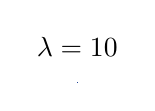
\begin{tikzpicture}[%
font=\footnotesize
]

\begin{axis}[%
width=0.951\figwidth,
height=\figheight,
at={(0\figwidth,0\figheight)},
scale only axis,
xmin=0,
xmax=3,
tick align=outside,
xlabel={Moneyness},
xmajorgrids,
ymin=0,
ymax=5,
ylabel={Remaining Time},
ymajorgrids,
zmin=0,
zmax=0.025,
zlabel={Optimal Rate},
zmajorgrids,
view={50}{40},
axis background/.style={fill=white},
title style={font=\bfseries},
title={$\lambda = 10$},
axis x line*=bottom,
axis y line*=left,
axis z line*=left
]

\addplot3[%
surf,
shader=flat corner,draw=black,z buffer=sort,colormap={mymap}{[1pt] rgb(0pt)=(0.2081,0.1663,0.5292); rgb(1pt)=(0.211624,0.189781,0.577676); rgb(2pt)=(0.212252,0.213771,0.626971); rgb(3pt)=(0.2081,0.2386,0.677086); rgb(4pt)=(0.195905,0.264457,0.7279); rgb(5pt)=(0.170729,0.291938,0.779248); rgb(6pt)=(0.125271,0.324243,0.830271); rgb(7pt)=(0.0591333,0.359833,0.868333); rgb(8pt)=(0.0116952,0.38751,0.881957); rgb(9pt)=(0.00595714,0.408614,0.882843); rgb(10pt)=(0.0165143,0.4266,0.878633); rgb(11pt)=(0.0328524,0.443043,0.871957); rgb(12pt)=(0.0498143,0.458571,0.864057); rgb(13pt)=(0.0629333,0.47369,0.855438); rgb(14pt)=(0.0722667,0.488667,0.8467); rgb(15pt)=(0.0779429,0.503986,0.838371); rgb(16pt)=(0.0793476,0.520024,0.831181); rgb(17pt)=(0.0749429,0.537543,0.826271); rgb(18pt)=(0.0640571,0.556986,0.823957); rgb(19pt)=(0.0487714,0.577224,0.822829); rgb(20pt)=(0.0343429,0.596581,0.819852); rgb(21pt)=(0.0265,0.6137,0.8135); rgb(22pt)=(0.0238905,0.628662,0.803762); rgb(23pt)=(0.0230905,0.641786,0.791267); rgb(24pt)=(0.0227714,0.653486,0.776757); rgb(25pt)=(0.0266619,0.664195,0.760719); rgb(26pt)=(0.0383714,0.674271,0.743552); rgb(27pt)=(0.0589714,0.683757,0.725386); rgb(28pt)=(0.0843,0.692833,0.706167); rgb(29pt)=(0.113295,0.7015,0.685857); rgb(30pt)=(0.145271,0.709757,0.664629); rgb(31pt)=(0.180133,0.717657,0.642433); rgb(32pt)=(0.217829,0.725043,0.619262); rgb(33pt)=(0.258643,0.731714,0.595429); rgb(34pt)=(0.302171,0.737605,0.571186); rgb(35pt)=(0.348167,0.742433,0.547267); rgb(36pt)=(0.395257,0.7459,0.524443); rgb(37pt)=(0.44201,0.748081,0.503314); rgb(38pt)=(0.487124,0.749062,0.483976); rgb(39pt)=(0.530029,0.749114,0.466114); rgb(40pt)=(0.570857,0.748519,0.44939); rgb(41pt)=(0.609852,0.747314,0.433686); rgb(42pt)=(0.6473,0.7456,0.4188); rgb(43pt)=(0.683419,0.743476,0.404433); rgb(44pt)=(0.71841,0.741133,0.390476); rgb(45pt)=(0.752486,0.7384,0.376814); rgb(46pt)=(0.785843,0.735567,0.363271); rgb(47pt)=(0.818505,0.732733,0.34979); rgb(48pt)=(0.850657,0.7299,0.336029); rgb(49pt)=(0.882433,0.727433,0.3217); rgb(50pt)=(0.913933,0.725786,0.306276); rgb(51pt)=(0.944957,0.726114,0.288643); rgb(52pt)=(0.973895,0.731395,0.266648); rgb(53pt)=(0.993771,0.745457,0.240348); rgb(54pt)=(0.999043,0.765314,0.216414); rgb(55pt)=(0.995533,0.786057,0.196652); rgb(56pt)=(0.988,0.8066,0.179367); rgb(57pt)=(0.978857,0.827143,0.163314); rgb(58pt)=(0.9697,0.848138,0.147452); rgb(59pt)=(0.962586,0.870514,0.1309); rgb(60pt)=(0.958871,0.8949,0.113243); rgb(61pt)=(0.959824,0.921833,0.0948381); rgb(62pt)=(0.9661,0.951443,0.0755333); rgb(63pt)=(0.9763,0.9831,0.0538)},mesh/rows=25]
table[row sep=crcr, point meta=\thisrow{c}] {%
%
x	y	z	c\\
0	0.01	0.00291314074482373	0.00291314074482373\\
0	0.111836734693878	0.00333408635754715	0.00333408635754715\\
0	0.213673469387755	0.00369577264611717	0.00369577264611717\\
0	0.315510204081633	0.00404234565773096	0.00404234565773096\\
0	0.41734693877551	0.0043813235848794	0.0043813235848794\\
0	0.519183673469388	0.00471577151525561	0.00471577151525561\\
0	0.621020408163265	0.00504732078871617	0.00504732078871617\\
0	0.722857142857143	0.00537697688622667	0.00537697688622667\\
0	0.82469387755102	0.00570542211182945	0.00570542211182945\\
0	0.926530612244898	0.0060331526747075	0.0060331526747075\\
0	1.02836734693878	0.00636054904240984	0.00636054904240984\\
0	1.13020408163265	0.00668791543444266	0.00668791543444266\\
0	1.23204081632653	0.00701550354834704	0.00701550354834704\\
0	1.33387755102041	0.0073435275935312	0.0073435275935312\\
0	1.43571428571429	0.0076721742367277	0.0076721742367277\\
0	1.53755102040816	0.00800160941991116	0.00800160941991116\\
0	1.63938775510204	0.00833198317653776	0.00833198317653776\\
0	1.74122448979592	0.00866343312220568	0.00866343312220568\\
0	1.8430612244898	0.00899608704145686	0.00899608704145686\\
0	1.94489795918367	0.00933006484249267	0.00933006484249267\\
0	2.04673469387755	0.00966548005997781	0.00966548005997781\\
0	2.14857142857143	0.0100024410283798	0.0100024410283798\\
0	2.25040816326531	0.0103410518109175	0.0103410518109175\\
0	2.35224489795918	0.0106814129443863	0.0106814129443863\\
0	2.45408163265306	0.0110236220433183	0.0110236220433183\\
0	2.55591836734694	0.0113677742953105	0.0113677742953105\\
0	2.65775510204082	0.0117139628711771	0.0117139628711771\\
0	2.75959183673469	0.0120622792677445	0.0120622792677445\\
0	2.86142857142857	0.0124128135968573	0.0124128135968573\\
0	2.96326530612245	0.0127656548310612	0.0127656548310612\\
0	3.06510204081633	0.0131208910140978	0.0131208910140978\\
0	3.1669387755102	0.0134786094426121	0.0134786094426121\\
0	3.26877551020408	0.0138388968241436	0.0138388968241436\\
0	3.37061224489796	0.0142018394154475	0.0142018394154475\\
0	3.47244897959184	0.0145675231444132	0.0145675231444132\\
0	3.57428571428571	0.0149360337182245	0.0149360337182245\\
0	3.67612244897959	0.0153074567199188	0.0153074567199188\\
0	3.77795918367347	0.0156818776951198	0.0156818776951198\\
0	3.87979591836735	0.0160593822304132	0.0160593822304132\\
0	3.98163265306122	0.0164400560245783	0.0164400560245783\\
0	4.0834693877551	0.0168239849536973	0.0168239849536973\\
0	4.18530612244898	0.0172112551309927	0.0172112551309927\\
0	4.28714285714286	0.0176019529621191	0.0176019529621191\\
0	4.38897959183674	0.0179961651965142	0.0179961651965142\\
0	4.49081632653061	0.0183939789753308	0.0183939789753308\\
0	4.59265306122449	0.0187954818763992	0.0187954818763992\\
0	4.69448979591837	0.0192007619565926	0.0192007619565926\\
0	4.79632653061224	0.0196099077919291	0.0196099077919291\\
0	4.89816326530612	0.0200230085156958	0.0200230085156958\\
0	5	0.0204401538548354	0.0204401538548354\\
0.125	0.01	0.00285699767118217	0.00285699767118217\\
0.125	0.111836734693878	0.00320747280155247	0.00320747280155247\\
0.125	0.213673469387755	0.00355569206784787	0.00355569206784787\\
0.125	0.315510204081633	0.00389555028497027	0.00389555028497027\\
0.125	0.41734693877551	0.00423020666504739	0.00423020666504739\\
0.125	0.519183673469388	0.00456148993998993	0.00456148993998993\\
0.125	0.621020408163265	0.00489052805787527	0.00489052805787527\\
0.125	0.722857142857143	0.00521807792374322	0.00521807792374322\\
0.125	0.82469387755102	0.00554468307370448	0.00554468307370448\\
0.125	0.926530612244898	0.00587075532085358	0.00587075532085358\\
0.125	1.02836734693878	0.00619662043660472	0.00619662043660472\\
0.125	1.13020408163265	0.00652254540456413	0.00652254540456413\\
0.125	1.23204081632653	0.00684875555505589	0.00684875555505589\\
0.125	1.33387755102041	0.0071754458131195	0.0071754458131195\\
0.125	1.43571428571429	0.00750278835357977	0.00750278835357977\\
0.125	1.53755102040816	0.00783093797256019	0.00783093797256019\\
0.125	1.63938775510204	0.00816003595677975	0.00816003595677975\\
0.125	1.74122448979592	0.0084902129349091	0.0084902129349091\\
0.125	1.8430612244898	0.0088215910211538	0.0088215910211538\\
0.125	1.94489795918367	0.00915428545549307	0.00915428545549307\\
0.125	2.04673469387755	0.00948840587875141	0.00948840587875141\\
0.125	2.14857142857143	0.00982405733801129	0.00982405733801129\\
0.125	2.25040816326531	0.0101613410897122	0.0101613410897122\\
0.125	2.35224489795918	0.0105003551737617	0.0105003551737617\\
0.125	2.45408163265306	0.0108411953190582	0.0108411953190582\\
0.125	2.55591836734694	0.0111839546311443	0.0111839546311443\\
0.125	2.65775510204082	0.0115287247072299	0.0115287247072299\\
0.125	2.75959183673469	0.0118755955678125	0.0118755955678125\\
0.125	2.86142857142857	0.0122246559917089	0.0122246559917089\\
0.125	2.96326530612245	0.0125759937382378	0.0125759937382378\\
0.125	3.06510204081633	0.0129296957373453	0.0129296957373453\\
0.125	3.1669387755102	0.0132858482602306	0.0132858482602306\\
0.125	3.26877551020408	0.0136445370572738	0.0136445370572738\\
0.125	3.37061224489796	0.014005847489898	0.014005847489898\\
0.125	3.47244897959184	0.0143698646422484	0.0143698646422484\\
0.125	3.57428571428571	0.0147366734216053	0.0147366734216053\\
0.125	3.67612244897959	0.0151063586483697	0.0151063586483697\\
0.125	3.77795918367347	0.0154790051371857	0.0154790051371857\\
0.125	3.87979591836735	0.015854697770504	0.015854697770504\\
0.125	3.98163265306122	0.0162335215656681	0.0162335215656681\\
0.125	4.0834693877551	0.0166155617364336	0.0166155617364336\\
0.125	4.18530612244898	0.0170009037496876	0.0170009037496876\\
0.125	4.28714285714286	0.0173896333780127	0.0173896333780127\\
0.125	4.38897959183674	0.0177818367486505	0.0177818367486505\\
0.125	4.49081632653061	0.0181776003893315	0.0181776003893315\\
0.125	4.59265306122449	0.0185770112670668	0.0185770112670668\\
0.125	4.69448979591837	0.0189801568471945	0.0189801568471945\\
0.125	4.79632653061224	0.0193871251032387	0.0193871251032387\\
0.125	4.89816326530612	0.0197980045734949	0.0197980045734949\\
0.125	5	0.0202128843890495	0.0202128843890495\\
0.25	0.01	0.00285671424141006	0.00285671424141006\\
0.25	0.111836734693878	0.00315914016229041	0.00315914016229041\\
0.25	0.213673469387755	0.00348075083688025	0.00348075083688025\\
0.25	0.315510204081633	0.00380538280888421	0.00380538280888421\\
0.25	0.41734693877551	0.00412987480641283	0.00412987480641283\\
0.25	0.519183673469388	0.00445371425083096	0.00445371425083096\\
0.25	0.621020408163265	0.00477695645265042	0.00477695645265042\\
0.25	0.722857142857143	0.00509979124258681	0.00509979124258681\\
0.25	0.82469387755102	0.00542243107555782	0.00542243107555782\\
0.25	0.926530612244898	0.00574507992059228	0.00574507992059228\\
0.25	1.02836734693878	0.0060679256468955	0.0060679256468955\\
0.25	1.13020408163265	0.0063911396613486	0.0063911396613486\\
0.25	1.23204081632653	0.00671487867118519	0.00671487867118519\\
0.25	1.33387755102041	0.00703928687059682	0.00703928687059682\\
0.25	1.43571428571429	0.00736449799719024	0.00736449799719024\\
0.25	1.53755102040816	0.00769063710589025	0.00769063710589025\\
0.25	1.63938775510204	0.0080178220482057	0.0080178220482057\\
0.25	1.74122448979592	0.00834616468974385	0.00834616468974385\\
0.25	1.8430612244898	0.0086757719088033	0.0086757719088033\\
0.25	1.94489795918367	0.0090067464166142	0.0090067464166142\\
0.25	2.04673469387755	0.00933918743348472	0.00933918743348472\\
0.25	2.14857142857143	0.00967319124943385	0.00967319124943385\\
0.25	2.25040816326531	0.0100088516919126	0.0100088516919126\\
0.25	2.35224489795918	0.0103462605183166	0.0103462605183166\\
0.25	2.45408163265306	0.0106855077476954	0.0106855077476954\\
0.25	2.55591836734694	0.0110266819429571	0.0110266819429571\\
0.25	2.65775510204082	0.0113698704526949	0.0113698704526949\\
0.25	2.75959183673469	0.0117151596184378	0.0117151596184378\\
0.25	2.86142857142857	0.0120626349546262	0.0120626349546262\\
0.25	2.96326530612245	0.012412381311439	0.012412381311439\\
0.25	3.06510204081633	0.0127644830056971	0.0127644830056971\\
0.25	3.1669387755102	0.0131190239475174	0.0131190239475174\\
0.25	3.26877551020408	0.0134760877479449	0.0134760877479449\\
0.25	3.37061224489796	0.0138357578160264	0.0138357578160264\\
0.25	3.47244897959184	0.0141981174460685	0.0141981174460685\\
0.25	3.57428571428571	0.0145632498965077	0.0145632498965077\\
0.25	3.67612244897959	0.0149312384615916	0.0149312384615916\\
0.25	3.77795918367347	0.0153021665368742	0.0153021665368742\\
0.25	3.87979591836735	0.0156761176793743	0.0156761176793743\\
0.25	3.98163265306122	0.0160531756631134	0.0160531756631134\\
0.25	4.0834693877551	0.0164334245306444	0.0164334245306444\\
0.25	4.18530612244898	0.0168169486410923	0.0168169486410923\\
0.25	4.28714285714286	0.0172038327151525	0.0172038327151525\\
0.25	4.38897959183674	0.0175941618774322	0.0175941618774322\\
0.25	4.49081632653061	0.0179880216964656	0.0179880216964656\\
0.25	4.59265306122449	0.0183854982226906	0.0183854982226906\\
0.25	4.69448979591837	0.0187866780246361	0.0187866780246361\\
0.25	4.79632653061224	0.0191916482195035	0.0191916482195035\\
0.25	4.89816326530612	0.0196004965265741	0.0196004965265741\\
0.25	5	0.0200133112588858	0.0200133112588858\\
0.375	0.01	0.00285671423384934	0.00285671423384934\\
0.375	0.111836734693878	0.00314716240506799	0.00314716240506799\\
0.375	0.213673469387755	0.00344859266254764	0.00344859266254764\\
0.375	0.315510204081633	0.00375754591199711	0.00375754591199711\\
0.375	0.41734693877551	0.00407014462169625	0.00407014462169625\\
0.375	0.519183673469388	0.00438466876843967	0.00438466876843967\\
0.375	0.621020408163265	0.00470037179602297	0.00470037179602297\\
0.375	0.722857142857143	0.0050169332534188	0.0050169332534188\\
0.375	0.82469387755102	0.0053342318417944	0.0053342318417944\\
0.375	0.926530612244898	0.00565224515872741	0.00565224515872741\\
0.375	1.02836734693878	0.00597100218120087	0.00597100218120087\\
0.375	1.13020408163265	0.00629055936780714	0.00629055936780714\\
0.375	1.23204081632653	0.00661098806144019	0.00661098806144019\\
0.375	1.33387755102041	0.00693236760726375	0.00693236760726375\\
0.375	1.43571428571429	0.00725478149643949	0.00725478149643949\\
0.375	1.53755102040816	0.00757831517259096	0.00757831517259096\\
0.375	1.63938775510204	0.00790305477979987	0.00790305477979987\\
0.375	1.74122448979592	0.00822908645641662	0.00822908645641662\\
0.375	1.8430612244898	0.00855649595082881	0.00855649595082881\\
0.375	1.94489795918367	0.00888536842928459	0.00888536842928459\\
0.375	2.04673469387755	0.00921578839879064	0.00921578839879064\\
0.375	2.14857142857143	0.00954783969869365	0.00954783969869365\\
0.375	2.25040816326531	0.00988160553263058	0.00988160553263058\\
0.375	2.35224489795918	0.0102171685234175	0.0102171685234175\\
0.375	2.45408163265306	0.0105546107801064	0.0105546107801064\\
0.375	2.55591836734694	0.0108940139705657	0.0108940139705657\\
0.375	2.65775510204082	0.0112354593955249	0.0112354593955249\\
0.375	2.75959183673469	0.0115790280616498	0.0115790280616498\\
0.375	2.86142857142857	0.0119248007522482	0.0119248007522482\\
0.375	2.96326530612245	0.0122728580948565	0.0122728580948565\\
0.375	3.06510204081633	0.012623280625366	0.012623280625366\\
0.375	3.1669387755102	0.0129761488486056	0.0129761488486056\\
0.375	3.26877551020408	0.0133315432954506	0.0133315432954506\\
0.375	3.37061224489796	0.0136895445766184	0.0136895445766184\\
0.375	3.47244897959184	0.0140502334333588	0.0140502334333588\\
0.375	3.57428571428571	0.0144136907852732	0.0144136907852732\\
0.375	3.67612244897959	0.0147799977754982	0.0147799977754982\\
0.375	3.77795918367347	0.0151492358134876	0.0151492358134876\\
0.375	3.87979591836735	0.0155214866156161	0.0155214866156161\\
0.375	3.98163265306122	0.0158968322438119	0.0158968322438119\\
0.375	4.0834693877551	0.0162753551424149	0.0162753551424149\\
0.375	4.18530612244898	0.0166571381734367	0.0166571381734367\\
0.375	4.28714285714286	0.0170422646504298	0.0170422646504298\\
0.375	4.38897959183674	0.017430818370957	0.017430818370957\\
0.375	4.49081632653061	0.0178228836479467	0.0178228836479467\\
0.375	4.59265306122449	0.0182185453401542	0.0182185453401542\\
0.375	4.69448979591837	0.0186178888815654	0.0186178888815654\\
0.375	4.79632653061224	0.0190210003100233	0.0190210003100233\\
0.375	4.89816326530612	0.01942796629513	0.01942796629513\\
0.375	5	0.0198388741655041	0.0198388741655041\\
0.5	0.01	0.00285671423384934	0.00285671423384934\\
0.5	0.111836734693878	0.00314530325617736	0.00314530325617736\\
0.5	0.213673469387755	0.00343771741843681	0.00343771741843681\\
0.5	0.315510204081633	0.00373587059128708	0.00373587059128708\\
0.5	0.41734693877551	0.00403851681814378	0.00403851681814378\\
0.5	0.519183673469388	0.00434435472509938	0.00434435472509938\\
0.5	0.621020408163265	0.00465253479314368	0.00465253479314368\\
0.5	0.722857142857143	0.00496254555914794	0.00496254555914794\\
0.5	0.82469387755102	0.00527408752247147	0.00527408752247147\\
0.5	0.926530612244898	0.00558699154691453	0.00558699154691453\\
0.5	1.02836734693878	0.00590116985267885	0.00590116985267885\\
0.5	1.13020408163265	0.00621658658941909	0.00621658658941909\\
0.5	1.23204081632653	0.00653323983026839	0.00653323983026839\\
0.5	1.33387755102041	0.00685115029292515	0.00685115029292515\\
0.5	1.43571428571429	0.00717035410799371	0.00717035410799371\\
0.5	1.53755102040816	0.0074908980813044	0.0074908980813044\\
0.5	1.63938775510204	0.00781283652972964	0.00781283652972964\\
0.5	1.74122448979592	0.00813622913192654	0.00813622913192654\\
0.5	1.8430612244898	0.00846113944711677	0.00846113944711677\\
0.5	1.94489795918367	0.00878763388173136	0.00878763388173136\\
0.5	2.04673469387755	0.00911578096133161	0.00911578096133161\\
0.5	2.14857142857143	0.00944565081373966	0.00944565081373966\\
0.5	2.25040816326531	0.00977731480026548	0.00977731480026548\\
0.5	2.35224489795918	0.0101108452520278	0.0101108452520278\\
0.5	2.45408163265306	0.0104463152816551	0.0104463152816551\\
0.5	2.55591836734694	0.0107837986495699	0.0107837986495699\\
0.5	2.65775510204082	0.0111233696701328	0.0111233696701328\\
0.5	2.75959183673469	0.0114651031471076	0.0114651031471076\\
0.5	2.86142857142857	0.011809074330836	0.011809074330836\\
0.5	2.96326530612245	0.0121553588915728	0.0121553588915728\\
0.5	3.06510204081633	0.0125040329049061	0.0125040329049061\\
0.5	3.1669387755102	0.0128551728462481	0.0128551728462481\\
0.5	3.26877551020408	0.0132088555921516	0.0132088555921516\\
0.5	3.37061224489796	0.0135651584267728	0.0135651584267728\\
0.5	3.47244897959184	0.0139241590522173	0.0139241590522173\\
0.5	3.57428571428571	0.014285935601814	0.014285935601814\\
0.5	3.67612244897959	0.014650566655596	0.014650566655596\\
0.5	3.77795918367347	0.0150181312574383	0.0150181312574383\\
0.5	3.87979591836735	0.0153887089334352	0.0153887089334352\\
0.5	3.98163265306122	0.0157623797111999	0.0157623797111999\\
0.5	4.0834693877551	0.0161392241398452	0.0161392241398452\\
0.5	4.18530612244898	0.0165193233104611	0.0165193233104611\\
0.5	4.28714285714286	0.0169027588769508	0.0169027588769508\\
0.5	4.38897959183674	0.0172896130771224	0.0172896130771224\\
0.5	4.49081632653061	0.0176799687539563	0.0176799687539563\\
0.5	4.59265306122449	0.0180739093769932	0.0180739093769932\\
0.5	4.69448979591837	0.0184715190638004	0.0184715190638004\\
0.5	4.79632653061224	0.0188728826014879	0.0188728826014879\\
0.5	4.89816326530612	0.0192780854682544	0.0192780854682544\\
0.5	5	0.0196872138549518	0.0196872138549518\\
0.625	0.01	0.00285671423384934	0.00285671423384934\\
0.625	0.111836734693878	0.00314512660926459	0.00314512660926459\\
0.625	0.213673469387755	0.00343485446341211	0.00343485446341211\\
0.625	0.315510204081633	0.00372755225859538	0.00372755225859538\\
0.625	0.41734693877551	0.00402371333079019	0.00402371333079019\\
0.625	0.519183673469388	0.00432300705483323	0.00432300705483323\\
0.625	0.621020408163265	0.00462496822683108	0.00462496822683108\\
0.625	0.722857142857143	0.00492920669122176	0.00492920669122176\\
0.625	0.82469387755102	0.00523543644358793	0.00523543644358793\\
0.625	0.926530612244898	0.00554346026836502	0.00554346026836502\\
0.625	1.02836734693878	0.00585314861529262	0.00585314861529262\\
0.625	1.13020408163265	0.00616442179610002	0.00616442179610002\\
0.625	1.23204081632653	0.00647723661102806	0.00647723661102806\\
0.625	1.33387755102041	0.00679157666450327	0.00679157666450327\\
0.625	1.43571428571429	0.00710744541855347	0.00710744541855347\\
0.625	1.53755102040816	0.00742486120144092	0.00742486120144092\\
0.625	1.63938775510204	0.00774385359735776	0.00774385359735776\\
0.625	1.74122448979592	0.00806446081229648	0.00806446081229648\\
0.625	1.8430612244898	0.00838672773411841	0.00838672773411841\\
0.625	1.94489795918367	0.00871070449055285	0.00871070449055285\\
0.625	2.04673469387755	0.00903644536781205	0.00903644536781205\\
0.625	2.14857142857143	0.00936400799298778	0.00936400799298778\\
0.625	2.25040816326531	0.00969345271131019	0.00969345271131019\\
0.625	2.35224489795918	0.010024842108738	0.010024842108738\\
0.625	2.45408163265306	0.0103582406439337	0.0103582406439337\\
0.625	2.55591836734694	0.0106937143632866	0.0106937143632866\\
0.625	2.65775510204082	0.0110313306795049	0.0110313306795049\\
0.625	2.75959183673469	0.0113711581992458	0.0113711581992458\\
0.625	2.86142857142857	0.0117132665888493	0.0117132665888493\\
0.625	2.96326530612245	0.0120577264698833	0.0120577264698833\\
0.625	3.06510204081633	0.0124046093381631	0.0124046093381631\\
0.625	3.1669387755102	0.0127539875013691	0.0127539875013691\\
0.625	3.26877551020408	0.0131059340314823	0.0131059340314823\\
0.625	3.37061224489796	0.0134605227290938	0.0134605227290938\\
0.625	3.47244897959184	0.0138178280972758	0.0138178280972758\\
0.625	3.57428571428571	0.0141779253231919	0.0141779253231919\\
0.625	3.67612244897959	0.0145408902660021	0.0145408902660021\\
0.625	3.77795918367347	0.0149067994499111	0.0149067994499111\\
0.625	3.87979591836735	0.0152757300614372	0.0152757300614372\\
0.625	3.98163265306122	0.0156477599501629	0.0156477599501629\\
0.625	4.0834693877551	0.0160229676323678	0.0160229676323678\\
0.625	4.18530612244898	0.01640143229706	0.01640143229706\\
0.625	4.28714285714286	0.0167832338140122	0.0167832338140122\\
0.625	4.38897959183674	0.0171684527434821	0.0171684527434821\\
0.625	4.49081632653061	0.0175571703473537	0.0175571703473537\\
0.625	4.59265306122449	0.0179494686014847	0.0179494686014847\\
0.625	4.69448979591837	0.0183454302090845	0.0183454302090845\\
0.625	4.79632653061224	0.0187451386149746	0.0187451386149746\\
0.625	4.89816326530612	0.0191486780206144	0.0191486780206144\\
0.625	5	0.0195561333997914	0.0195561333997914\\
0.75	0.01	0.00285671423384934	0.00285671423384934\\
0.75	0.111836734693878	0.00314511649114392	0.00314511649114392\\
0.75	0.213673469387755	0.00343427283730026	0.00343427283730026\\
0.75	0.315510204081633	0.00372486511503283	0.00372486511503283\\
0.75	0.41734693877551	0.00401761787050039	0.00401761787050039\\
0.75	0.519183673469388	0.00431279439754599	0.00431279439754599\\
0.75	0.621020408163265	0.00461036019172466	0.00461036019172466\\
0.75	0.722857142857143	0.00491017497986613	0.00491017497986613\\
0.75	0.82469387755102	0.00521208524110943	0.00521208524110943\\
0.75	0.926530612244898	0.00551595841992711	0.00551595841992711\\
0.75	1.02836734693878	0.00582169189585285	0.00582169189585285\\
0.75	1.13020408163265	0.00612921233671354	0.00612921233671354\\
0.75	1.23204081632653	0.00643847195717221	0.00643847195717221\\
0.75	1.33387755102041	0.0067494442323409	0.0067494442323409\\
0.75	1.43571428571429	0.00706211997469628	0.00706211997469628\\
0.75	1.53755102040816	0.00737650402630658	0.00737650402630658\\
0.75	1.63938775510204	0.00769261256980771	0.00769261256980771\\
0.75	1.74122448979592	0.0080104709790969	0.0080104709790969\\
0.75	1.8430612244898	0.00833011211383518	0.00833011211383518\\
0.75	1.94489795918367	0.00865157496893904	0.00865157496893904\\
0.75	2.04673469387755	0.00897490360435214	0.00897490360435214\\
0.75	2.14857142857143	0.00930014629494469	0.00930014629494469\\
0.75	2.25040816326531	0.00962735485313404	0.00962735485313404\\
0.75	2.35224489795918	0.00995658408724493	0.00995658408724493\\
0.75	2.45408163265306	0.0102878913668769	0.0102878913668769\\
0.75	2.55591836734694	0.0106213362729657	0.0106213362729657\\
0.75	2.65775510204082	0.0109569803151814	0.0109569803151814\\
0.75	2.75959183673469	0.0112948867031187	0.0112948867031187\\
0.75	2.86142857142857	0.0116351201606719	0.0116351201606719\\
0.75	2.96326530612245	0.0119777467752482	0.0119777467752482\\
0.75	3.06510204081633	0.012322833875225	0.012322833875225\\
0.75	3.1669387755102	0.0126704499304143	0.0126704499304143\\
0.75	3.26877551020408	0.0130206644713579	0.0130206644713579\\
0.75	3.37061224489796	0.0133735480241043	0.0133735480241043\\
0.75	3.47244897959184	0.0137291720577732	0.0137291720577732\\
0.75	3.57428571428571	0.0140876089427264	0.0140876089427264\\
0.75	3.67612244897959	0.0144489319175768	0.0144489319175768\\
0.75	3.77795918367347	0.0148132150635884	0.0148132150635884\\
0.75	3.87979591836735	0.0151805332852881	0.0151805332852881\\
0.75	3.98163265306122	0.0155509622963147	0.0155509622963147\\
0.75	4.0834693877551	0.015924578609705	0.015924578609705\\
0.75	4.18530612244898	0.0163014595319507	0.0163014595319507\\
0.75	4.28714285714286	0.0166816831602779	0.0166816831602779\\
0.75	4.38897959183674	0.0170653283826859	0.0170653283826859\\
0.75	4.49081632653061	0.0174524748803629	0.0174524748803629\\
0.75	4.59265306122449	0.017843203132157	0.017843203132157\\
0.75	4.69448979591837	0.01823759442083	0.01823759442083\\
0.75	4.79632653061224	0.0186357308408669	0.0186357308408669\\
0.75	4.89816326530612	0.019037695307649	0.019037695307649\\
0.75	5	0.019443571567826	0.019443571567826\\
0.875	0.01	0.00285671423384934	0.00285671423384934\\
0.875	0.111836734693878	0.00314511614550906	0.00314511614550906\\
0.875	0.213673469387755	0.00343418221982576	0.00343418221982576\\
0.875	0.315510204081633	0.00372413779940329	0.00372413779940329\\
0.875	0.41734693877551	0.00401541798419736	0.00401541798419736\\
0.875	0.519183673469388	0.00430839393574358	0.00430839393574358\\
0.875	0.621020408163265	0.00460326010363736	0.00460326010363736\\
0.875	0.722857142857143	0.00490008012640724	0.00490008012640724\\
0.875	0.82469387755102	0.00519884887875936	0.00519884887875936\\
0.875	0.926530612244898	0.0054995333825573	0.0054995333825573\\
0.875	1.02836734693878	0.00580209490881961	0.00580209490881961\\
0.875	1.13020408163265	0.00610649961101357	0.00610649961101357\\
0.875	1.23204081632653	0.00641272296383277	0.00641272296383277\\
0.875	1.33387755102041	0.00672075106407066	0.00672075106407066\\
0.875	1.43571428571429	0.00703058043575697	0.00703058043575697\\
0.875	1.53755102040816	0.00734221718940327	0.00734221718940327\\
0.875	1.63938775510204	0.00765567596214471	0.00765567596214471\\
0.875	1.74122448979592	0.00797097884452536	0.00797097884452536\\
0.875	1.8430612244898	0.00828815438587877	0.00828815438587877\\
0.875	1.94489795918367	0.00860723671272729	0.00860723671272729\\
0.875	2.04673469387755	0.00892826476644038	0.00892826476644038\\
0.875	2.14857142857143	0.00925128165340762	0.00925128165340762\\
0.875	2.25040816326531	0.0095763340957661	0.0095763340957661\\
0.875	2.35224489795918	0.00990347196937622	0.00990347196937622\\
0.875	2.45408163265306	0.0102327479162245	0.0102327479162245\\
0.875	2.55591836734694	0.0105642170196932	0.0105642170196932\\
0.875	2.65775510204082	0.0108979365326397	0.0108979365326397\\
0.875	2.75959183673469	0.0112339656497162	0.0112339656497162\\
0.875	2.86142857142857	0.0115723653167169	0.0115723653167169\\
0.875	2.96326530612245	0.0119131980709255	0.0119131980709255\\
0.875	3.06510204081633	0.0122565279074488	0.0122565279074488\\
0.875	3.1669387755102	0.0126024201673709	0.0126024201673709\\
0.875	3.26877551020408	0.0129509414442701	0.0129509414442701\\
0.875	3.37061224489796	0.0133021595062281	0.0133021595062281\\
0.875	3.47244897959184	0.013656143230943	0.013656143230943\\
0.875	3.57428571428571	0.01401296255196	0.01401296255196\\
0.875	3.67612244897959	0.0143726884143591	0.0143726884143591\\
0.875	3.77795918367347	0.0147353927385138	0.0147353927385138\\
0.875	3.87979591836735	0.0151011483907582	0.0151011483907582\\
0.875	3.98163265306122	0.0154700291599858	0.0154700291599858\\
0.875	4.0834693877551	0.0158421097393568	0.0158421097393568\\
0.875	4.18530612244898	0.0162174657124205	0.0162174657124205\\
0.875	4.28714285714286	0.0165961735430647	0.0165961735430647\\
0.875	4.38897959183674	0.0169783105687928	0.0169783105687928\\
0.875	4.49081632653061	0.0173639549969062	0.0173639549969062\\
0.875	4.59265306122449	0.0177531859032288	0.0177531859032288\\
0.875	4.69448979591837	0.0181460832330674	0.0181460832330674\\
0.875	4.79632653061224	0.0185427278041415	0.0185427278041415\\
0.875	4.89816326530612	0.0189432013112574	0.0189432013112574\\
0.875	5	0.0193475863325318	0.0193475863325318\\
1	0.01	0.00285671423384934	0.00285671423384934\\
1	0.111836734693878	0.00314511613852319	0.00314511613852319\\
1	0.213673469387755	0.00343417144235276	0.00343417144235276\\
1	0.315510204081633	0.00372397343285809	0.00372397343285809\\
1	0.41734693877551	0.00401472406907677	0.00401472406907677\\
1	0.519183673469388	0.00430669028138833	0.00430669028138833\\
1	0.621020408163265	0.00460010152799131	0.00460010152799131\\
1	0.722857142857143	0.00489511400390281	0.00489511400390281\\
1	0.82469387755102	0.00519182100003769	0.00519182100003769\\
1	0.926530612244898	0.00549027388961511	0.00549027388961511\\
1	1.02836734693878	0.0057904999584877	0.0057904999584877\\
1	1.13020408163265	0.00609251464995632	0.00609251464995632\\
1	1.23204081632653	0.00639632919193655	0.00639632919193655\\
1	1.33387755102041	0.0067019550496562	0.0067019550496562\\
1	1.43571428571429	0.00700940636036646	0.00700940636036646\\
1	1.53755102040816	0.00731870113956284	0.00731870113956284\\
1	1.63938775510204	0.00762986176304265	0.00762986176304265\\
1	1.74122448979592	0.00794291503640172	0.00794291503640172\\
1	1.8430612244898	0.00825789204064593	0.00825789204064593\\
1	1.94489795918367	0.00857482786631664	0.00857482786631664\\
1	2.04673469387755	0.00889376130187971	0.00889376130187971\\
1	2.14857142857143	0.00921473451385372	0.00921473451385372\\
1	2.25040816326531	0.00953779273915019	0.00953779273915019\\
1	2.35224489795918	0.00986298399997095	0.00986298399997095\\
1	2.45408163265306	0.0101903588456617	0.0101903588456617\\
1	2.55591836734694	0.0105199701225112	0.0105199701225112\\
1	2.65775510204082	0.0108518727706042	0.0108518727706042\\
1	2.75959183673469	0.0111861236458763	0.0111861236458763\\
1	2.86142857142857	0.011522781365094	0.011522781365094\\
1	2.96326530612245	0.0118619061713785	0.0118619061713785\\
1	3.06510204081633	0.0122035598179562	0.0122035598179562\\
1	3.1669387755102	0.0125478054679762	0.0125478054679762\\
1	3.26877551020408	0.0128947076084315	0.0128947076084315\\
1	3.37061224489796	0.0132443319764294	0.0132443319764294\\
1	3.47244897959184	0.0135967454962612	0.0135967454962612\\
1	3.57428571428571	0.0139520162259089	0.0139520162259089\\
1	3.67612244897959	0.0143102133118034	0.0143102133118034\\
1	3.77795918367347	0.0146714069507985	0.0146714069507985\\
1	3.87979591836735	0.0150356683584652	0.0150356683584652\\
1	3.98163265306122	0.0154030697429283	0.0154030697429283\\
1	4.0834693877551	0.0157736842835699	0.0157736842835699\\
1	4.18530612244898	0.0161475861140165	0.0161475861140165\\
1	4.28714285714286	0.0165248503089039	0.0165248503089039\\
1	4.38897959183674	0.0169055528739784	0.0169055528739784\\
1	4.49081632653061	0.0172897707391555	0.0172897707391555\\
1	4.59265306122449	0.0176775817542029	0.0176775817542029\\
1	4.69448979591837	0.0180690646867612	0.0180690646867612\\
1	4.79632653061224	0.0184642992224501	0.0184642992224501\\
1	4.89816326530612	0.0188633659668427	0.0188633659668427\\
1	5	0.0192663464491154	0.0192663464491154\\
1.125	0.01	0.00285671423384934	0.00285671423384934\\
1.125	0.111836734693878	0.00314511613844015	0.00314511613844015\\
1.125	0.213673469387755	0.00343417046726378	0.00343417046726378\\
1.125	0.315510204081633	0.00372394250181192	0.00372394250181192\\
1.125	0.41734693877551	0.00401453319206247	0.00401453319206247\\
1.125	0.519183673469388	0.00430609878353469	0.00430609878353469\\
1.125	0.621020408163265	0.00459881759972745	0.00459881759972745\\
1.125	0.722857142857143	0.00489285157191164	0.00489285157191164\\
1.125	0.82469387755102	0.00518833052219174	0.00518833052219174\\
1.125	0.926530612244898	0.0054853527587229	0.0054853527587229\\
1.125	1.02836734693878	0.00578399183799653	0.00578399183799653\\
1.125	1.13020408163265	0.00608430405233135	0.00608430405233135\\
1.125	1.23204081632653	0.00638633467625648	0.00638633467625648\\
1.125	1.33387755102041	0.00669012260676085	0.00669012260676085\\
1.125	1.43571428571429	0.00699570360002794	0.00699570360002794\\
1.125	1.53755102040816	0.00730311243544495	0.00730311243544495\\
1.125	1.63938775510204	0.00761238431072537	0.00761238431072537\\
1.125	1.74122448979592	0.007923555705709	0.007923555705709\\
1.125	1.8430612244898	0.00823666488782078	0.00823666488782078\\
1.125	1.94489795918367	0.00855175218053747	0.00855175218053747\\
1.125	2.04673469387755	0.00886886007816894	0.00886886007816894\\
1.125	2.14857142857143	0.00918803326334815	0.00918803326334815\\
1.125	2.25040816326531	0.0095093185650058	0.0095093185650058\\
1.125	2.35224489795918	0.00983276488188836	0.00983276488188836\\
1.125	2.45408163265306	0.010158423088061	0.010158423088061\\
1.125	2.55591836734694	0.0104863459310289	0.0104863459310289\\
1.125	2.65775510204082	0.0108165879292149	0.0108165879292149\\
1.125	2.75959183673469	0.0111492052729296	0.0111492052729296\\
1.125	2.86142857142857	0.0114842557312467	0.0114842557312467\\
1.125	2.96326530612245	0.0118217985660608	0.0118217985660608\\
1.125	3.06510204081633	0.0121618944538703	0.0121618944538703\\
1.125	3.1669387755102	0.0125046054153601	0.0125046054153601\\
1.125	3.26877551020408	0.0128499947525701	0.0128499947525701\\
1.125	3.37061224489796	0.0131981269932653	0.0131981269932653\\
1.125	3.47244897959184	0.0135490678420366	0.0135490678420366\\
1.125	3.57428571428571	0.0139028841376174	0.0139028841376174\\
1.125	3.67612244897959	0.0142596438159	0.0142596438159\\
1.125	3.77795918367347	0.0146194158781463	0.0146194158781463\\
1.125	3.87979591836735	0.0149822703639173	0.0149822703639173\\
1.125	3.98163265306122	0.0153482783282747	0.0153482783282747\\
1.125	4.0834693877551	0.0157175118228469	0.0157175118228469\\
1.125	4.18530612244898	0.0160900438803858	0.0160900438803858\\
1.125	4.28714285714286	0.0164659485024768	0.0164659485024768\\
1.125	4.38897959183674	0.0168453006500967	0.0168453006500967\\
1.125	4.49081632653061	0.0172281762367472	0.0172281762367472\\
1.125	4.59265306122449	0.0176146521239169	0.0176146521239169\\
1.125	4.69448979591837	0.0180048061186543	0.0180048061186543\\
1.125	4.79632653061224	0.0183987169730548	0.0183987169730548\\
1.125	4.89816326530612	0.018796464385488	0.018796464385488\\
1.125	5	0.0191981290034086	0.0191981290034086\\
1.25	0.01	0.00285671423384934	0.00285671423384934\\
1.25	0.111836734693878	0.00314511613843957	0.00314511613843957\\
1.25	0.213673469387755	0.00343417040033415	0.00343417040033415\\
1.25	0.315510204081633	0.00372393766505887	0.00372393766505887\\
1.25	0.41734693877551	0.00401448748618693	0.00401448748618693\\
1.25	0.519183673469388	0.00430591490051027	0.00430591490051027\\
1.25	0.621020408163265	0.00459834137172492	0.00459834137172492\\
1.25	0.722857142857143	0.00489189825794938	0.00489189825794938\\
1.25	0.82469387755102	0.0051867107275822	0.0051867107275822\\
1.25	0.926530612244898	0.00548288962232852	0.00548288962232852\\
1.25	1.02836734693878	0.0057805298025092	0.0057805298025092\\
1.25	1.13020408163265	0.00607971186012114	0.00607971186012114\\
1.25	1.23204081632653	0.00638050501621531	0.00638050501621531\\
1.25	1.33387755102041	0.0066829700778278	0.0066829700778278\\
1.25	1.43571428571429	0.00698716199662948	0.00698716199662948\\
1.25	1.53755102040816	0.00729313191073151	0.00729313191073151\\
1.25	1.63938775510204	0.00760092869844725	0.00760092869844725\\
1.25	1.74122448979592	0.00791060012360778	0.00791060012360778\\
1.25	1.8430612244898	0.00822219365937649	0.00822219365937649\\
1.25	1.94489795918367	0.0085357570679072	0.0085357570679072\\
1.25	2.04673469387755	0.00885133879882716	0.00885133879882716\\
1.25	2.14857142857143	0.00916898825548504	0.00916898825548504\\
1.25	2.25040816326531	0.00948875596596321	0.00948875596596321\\
1.25	2.35224489795918	0.00981069368634648	0.00981069368634648\\
1.25	2.45408163265306	0.0101348544564396	0.0101348544564396\\
1.25	2.55591836734694	0.0104612926226409	0.0104612926226409\\
1.25	2.65775510204082	0.0107900638386117	0.0107900638386117\\
1.25	2.75959183673469	0.0111212250513904	0.0111212250513904\\
1.25	2.86142857142857	0.011454834478415	0.011454834478415\\
1.25	2.96326530612245	0.0117909515793262	0.0117909515793262\\
1.25	3.06510204081633	0.0121296370252677	0.0121296370252677\\
1.25	3.1669387755102	0.0124709526675653	0.0124709526675653\\
1.25	3.26877551020408	0.0128149615070629	0.0128149615070629\\
1.25	3.37061224489796	0.0131617276649623	0.0131617276649623\\
1.25	3.47244897959184	0.0135113163557002	0.0135113163557002\\
1.25	3.57428571428571	0.0138637938621812	0.0138637938621812\\
1.25	3.67612244897959	0.0142192275135247	0.0142192275135247\\
1.25	3.77795918367347	0.0145776856653818	0.0145776856653818\\
1.25	3.87979591836735	0.014939237682801	0.014939237682801\\
1.25	3.98163265306122	0.0153039539255749	0.0153039539255749\\
1.25	4.0834693877551	0.0156719057359671	0.0156719057359671\\
1.25	4.18530612244898	0.0160431654287027	0.0160431654287027\\
1.25	4.28714285714286	0.016417806283094	0.016417806283094\\
1.25	4.38897959183674	0.0167959025371711	0.0167959025371711\\
1.25	4.49081632653061	0.0171775293836861	0.0171775293836861\\
1.25	4.59265306122449	0.0175627629678676	0.0175627629678676\\
1.25	4.69448979591837	0.0179516803868017	0.0179516803868017\\
1.25	4.79632653061224	0.0183443596903284	0.0183443596903284\\
1.25	4.89816326530612	0.0187408798833465	0.0187408798833465\\
1.25	5	0.0191413209294266	0.0191413209294266\\
1.375	0.01	0.00285671423384934	0.00285671423384934\\
1.375	0.111836734693878	0.00314511613843957	0.00314511613843957\\
1.375	0.213673469387755	0.00343417039685634	0.00343417039685634\\
1.375	0.315510204081633	0.0037239370376273	0.0037239370376273\\
1.375	0.41734693877551	0.00401447797261284	0.00401447797261284\\
1.375	0.519183673469388	0.00430586377921636	0.00430586377921636\\
1.375	0.621020408163265	0.00459818037239568	0.00459818037239568\\
1.375	0.722857142857143	0.00489152710477381	0.00489152710477381\\
1.375	0.82469387755102	0.0051860090456836	0.0051860090456836\\
1.375	0.926530612244898	0.00548172956602651	0.00548172956602651\\
1.375	1.02836734693878	0.00577878581370912	0.00577878581370912\\
1.375	1.13020408163265	0.00607726693132727	0.00607726693132727\\
1.375	1.23204081632653	0.00637725405734474	0.00637725405734474\\
1.375	1.33387755102041	0.00667882124313498	0.00667882124313498\\
1.375	1.43571428571429	0.00698203671511333	0.00698203671511333\\
1.375	1.53755102040816	0.00728696416514732	0.00728696416514732\\
1.375	1.63938775510204	0.00759366391874159	0.00759366391874159\\
1.375	1.74122448979592	0.00790219392578614	0.00790219392578614\\
1.375	1.8430612244898	0.00821261056792541	0.00821261056792541\\
1.375	1.94489795918367	0.00852496929913194	0.00852496929913194\\
1.375	2.04673469387755	0.00883932514419767	0.00883932514419767\\
1.375	2.14857142857143	0.00915573308079878	0.00915573308079878\\
1.375	2.25040816326531	0.00947424832851593	0.00947424832851593\\
1.375	2.35224489795918	0.00979492656477032	0.00979492656477032\\
1.375	2.45408163265306	0.010117824084083	0.010117824084083\\
1.375	2.55591836734694	0.0104429979138268	0.0104429979138268\\
1.375	2.65775510204082	0.0107705058968772	0.0107705058968772\\
1.375	2.75959183673469	0.0111004067492945	0.0111004067492945\\
1.375	2.86142857142857	0.0114327600993448	0.0114327600993448\\
1.375	2.96326530612245	0.0117676265127212	0.0117676265127212\\
1.375	3.06510204081633	0.0121050675076959	0.0121050675076959\\
1.375	3.1669387755102	0.0124451455630503	0.0124451455630503\\
1.375	3.26877551020408	0.0127879241209528	0.0127879241209528\\
1.375	3.37061224489796	0.0131334675864231	0.0131334675864231\\
1.375	3.47244897959184	0.0134818413246223	0.0134818413246223\\
1.375	3.57428571428571	0.0138331116568919	0.0138331116568919\\
1.375	3.67612244897959	0.0141873458562327	0.0141873458562327\\
1.375	3.77795918367347	0.0145446121427279	0.0145446121427279\\
1.375	3.87979591836735	0.0149049796792785	0.0149049796792785\\
1.375	3.98163265306122	0.0152685185679137	0.0152685185679137\\
1.375	4.0834693877551	0.0156352998468567	0.0156352998468567\\
1.375	4.18530612244898	0.0160053954884688	0.0160053954884688\\
1.375	4.28714285714286	0.0163788783981468	0.0163788783981468\\
1.375	4.38897959183674	0.0167558224142172	0.0167558224142172\\
1.375	4.49081632653061	0.0171363023088437	0.0171363023088437\\
1.375	4.59265306122449	0.017520393789947	0.017520393789947\\
1.375	4.69448979591837	0.0179081735041247	0.0179081735041247\\
1.375	4.79632653061224	0.0182997190405468	0.0182997190405468\\
1.375	4.89816326530612	0.0186951089357981	0.0186951089357981\\
1.375	5	0.0190944226796364	0.0190944226796364\\
1.5	0.01	0.00285671423384934	0.00285671423384934\\
1.5	0.111836734693878	0.00314511613843957	0.00314511613843957\\
1.5	0.213673469387755	0.00343417039671977	0.00343417039671977\\
1.5	0.315510204081633	0.0037239369701983	0.0037239369701983\\
1.5	0.41734693877551	0.00401447625325233	0.00401447625325233\\
1.5	0.519183673469388	0.00430585108262024	0.00430585108262024\\
1.5	0.621020408163265	0.0045981308087189	0.0045981308087189\\
1.5	0.722857142857143	0.00489139370467138	0.00489139370467138\\
1.5	0.82469387755102	0.00518572552635572	0.00518572552635572\\
1.5	0.926530612244898	0.00548121585712553	0.00548121585712553\\
1.5	1.02836734693878	0.00577795444702948	0.00577795444702948\\
1.5	1.13020408163265	0.00607602861628359	0.00607602861628359\\
1.5	1.23204081632653	0.00637552185130247	0.00637552185130247\\
1.5	1.33387755102041	0.00667651332568889	0.00667651332568889\\
1.5	1.43571428571429	0.00697907801436669	0.00697907801436669\\
1.5	1.53755102040816	0.00728328713166007	0.00728328713166007\\
1.5	1.63938775510204	0.00758920870994803	0.00758920870994803\\
1.5	1.74122448979592	0.00789690820730077	0.00789690820730077\\
1.5	1.8430612244898	0.00820644908294662	0.00820644908294662\\
1.5	1.94489795918367	0.00851789331158521	0.00851789331158521\\
1.5	2.04673469387755	0.0088313018266401	0.0088313018266401\\
1.5	2.14857142857143	0.00914673489306051	0.00914673489306051\\
1.5	2.25040816326531	0.00946425241552454	0.00946425241552454\\
1.5	2.35224489795918	0.00978391419005009	0.00978391419005009\\
1.5	2.45408163265306	0.0101057801074574	0.0101057801074574\\
1.5	2.55591836734694	0.0104299103166801	0.0104299103166801\\
1.5	2.65775510204082	0.0107563653550713	0.0107563653550713\\
1.5	2.75959183673469	0.011085206251877	0.011085206251877\\
1.5	2.86142857142857	0.011416494610078	0.011416494610078\\
1.5	2.96326530612245	0.0117502926709251	0.0117502926709251\\
1.5	3.06510204081633	0.0120866633647169	0.0120866633647169\\
1.5	3.1669387755102	0.0124256703507116	0.0124256703507116\\
1.5	3.26877551020408	0.012767378048515	0.012767378048515\\
1.5	3.37061224489796	0.0131118516628328	0.0131118516628328\\
1.5	3.47244897959184	0.0134591572031008	0.0134591572031008\\
1.5	3.57428571428571	0.0138093614992063	0.0138093614992063\\
1.5	3.67612244897959	0.0141625322142686	0.0141625322142686\\
1.5	3.77795918367347	0.0145187378552473	0.0145187378552473\\
1.5	3.87979591836735	0.0148780477819904	0.0148780477819904\\
1.5	3.98163265306122	0.0152405322152037	0.0152405322152037\\
1.5	4.0834693877551	0.0156062622437239	0.0156062622437239\\
1.5	4.18530612244898	0.0159753098313926	0.0159753098313926\\
1.5	4.28714285714286	0.0163477478237656	0.0163477478237656\\
1.5	4.38897959183674	0.0167236499548375	0.0167236499548375\\
1.5	4.49081632653061	0.0171030908539223	0.0171030908539223\\
1.5	4.59265306122449	0.017486146052795	0.017486146052795\\
1.5	4.69448979591837	0.0178728919931749	0.0178728919931749\\
1.5	4.79632653061224	0.0182634060346098	0.0182634060346098\\
1.5	4.89816326530612	0.0186577664628035	0.0186577664628035\\
1.5	5	0.0190560524984173	0.0190560524984173\\
1.625	0.01	0.00285671423384934	0.00285671423384934\\
1.625	0.111836734693878	0.00314511613843957	0.00314511613843957\\
1.625	0.213673469387755	0.00343417039671572	0.00343417039671572\\
1.625	0.315510204081633	0.00372393696420156	0.00372393696420156\\
1.625	0.41734693877551	0.00401447598370841	0.00401447598370841\\
1.625	0.519183673469388	0.0043058482679413	0.0043058482679413\\
1.625	0.621020408163265	0.00459811692530454	0.00459811692530454\\
1.625	0.722857142857143	0.00489134947295472	0.00489134947295472\\
1.625	0.82469387755102	0.0051856187444613	0.0051856187444613\\
1.625	0.926530612244898	0.00548100209469305	0.00548100209469305\\
1.625	1.02836734693878	0.00577757962683373	0.00577757962683373\\
1.625	1.13020408163265	0.00607543230455087	0.00607543230455087\\
1.625	1.23204081632653	0.00637464044115999	0.00637464044115999\\
1.625	1.33387755102041	0.00667528270759163	0.00667528270759163\\
1.625	1.43571428571429	0.00697743561013693	0.00697743561013693\\
1.625	1.53755102040816	0.00728117332200601	0.00728117332200601\\
1.625	1.63938775510204	0.00758656775049323	0.00758656775049323\\
1.625	1.74122448979592	0.00789368874394421	0.00789368874394421\\
1.625	1.8430612244898	0.00820260436955143	0.00820260436955143\\
1.625	1.94489795918367	0.00851338121622537	0.00851338121622537\\
1.625	2.04673469387755	0.00882608469433486	0.00882608469433486\\
1.625	2.14857142857143	0.00914077931636615	0.00914077931636615\\
1.625	2.25040816326531	0.00945752895064138	0.00945752895064138\\
1.625	2.35224489795918	0.00977639704531811	0.00977639704531811\\
1.625	2.45408163265306	0.0100974468229119	0.0100974468229119\\
1.625	2.55591836734694	0.0104207414472512	0.0104207414472512\\
1.625	2.65775510204082	0.0107463441655787	0.0107463441655787\\
1.625	2.75959183673469	0.0110743184287958	0.0110743184287958\\
1.625	2.86142857142857	0.0114047279928217	0.0114047279928217\\
1.625	2.96326530612245	0.011737637003843	0.011737637003843\\
1.625	3.06510204081633	0.012073110069965	0.012073110069965\\
1.625	3.1669387755102	0.0124112123214705	0.0124112123214705\\
1.625	3.26877551020408	0.0127520094616029	0.0127520094616029\\
1.625	3.37061224489796	0.0130955678095106	0.0130955678095106\\
1.625	3.47244897959184	0.0134419543367447	0.0134419543367447\\
1.625	3.57428571428571	0.0137912366984812	0.0137912366984812\\
1.625	3.67612244897959	0.0141434832604517	0.0141434832604517\\
1.625	3.77795918367347	0.0144987631224021	0.0144987631224021\\
1.625	3.87979591836735	0.0148571461387629	0.0148571461387629\\
1.625	3.98163265306122	0.0152187029370993	0.0152187029370993\\
1.625	4.0834693877551	0.0155835049348088	0.0155835049348088\\
1.625	4.18530612244898	0.0159516243544569	0.0159516243544569\\
1.625	4.28714285714286	0.0163231342380688	0.0163231342380688\\
1.625	4.38897959183674	0.0166981084606432	0.0166981084606432\\
1.625	4.49081632653061	0.0170766217431042	0.0170766217431042\\
1.625	4.59265306122449	0.0174587496648683	0.0174587496648683\\
1.625	4.69448979591837	0.0178445686761743	0.0178445686761743\\
1.625	4.79632653061224	0.0182341561102936	0.0182341561102936\\
1.625	4.89816326530612	0.0186275901957189	0.0186275901957189\\
1.625	5	0.01902495006841	0.01902495006841\\
1.75	0.01	0.00285671423384934	0.00285671423384934\\
1.75	0.111836734693878	0.00314511613843957	0.00314511613843957\\
1.75	0.213673469387755	0.00343417039671563	0.00343417039671563\\
1.75	0.315510204081633	0.00372393696376063	0.00372393696376063\\
1.75	0.41734693877551	0.00401447594708246	0.00401447594708246\\
1.75	0.519183673469388	0.00430584771137309	0.00430584771137309\\
1.75	0.621020408163265	0.00459811338908237	0.00459811338908237\\
1.75	0.722857142857143	0.00489133595149827	0.00489133595149827\\
1.75	0.82469387755102	0.0051855812782801	0.0051855812782801\\
1.75	0.926530612244898	0.00548091855541581	0.00548091855541581\\
1.75	1.02836734693878	0.00577741988593512	0.00577741988593512\\
1.75	1.13020408163265	0.00607515941609762	0.00607515941609762\\
1.75	1.23204081632653	0.006374212337446	0.006374212337446\\
1.75	1.33387755102041	0.00667465400411508	0.00667465400411508\\
1.75	1.43571428571429	0.00697655926923005	0.00697655926923005\\
1.75	1.53755102040816	0.00728000205340464	0.00728000205340464\\
1.75	1.63938775510204	0.00758505511327763	0.00758505511327763\\
1.75	1.74122448979592	0.00789178996323536	0.00789178996323536\\
1.75	1.8430612244898	0.00820027690455249	0.00820027690455249\\
1.75	1.94489795918367	0.00851058512378523	0.00851058512378523\\
1.75	2.04673469387755	0.0088227828313385	0.0088227828313385\\
1.75	2.14857142857143	0.00913693741941898	0.00913693741941898\\
1.75	2.25040816326531	0.00945311562529694	0.00945311562529694\\
1.75	2.35224489795918	0.00977138369086561	0.00977138369086561\\
1.75	2.45408163265306	0.0100918075131297	0.0100918075131297\\
1.75	2.55591836734694	0.0104144527827746	0.0104144527827746\\
1.75	2.65775510204082	0.0107393851096468	0.0107393851096468\\
1.75	2.75959183673469	0.0110666701350537	0.0110666701350537\\
1.75	2.86142857142857	0.0113963736314432	0.0113963736314432\\
1.75	2.96326530612245	0.0117285615903915	0.0117285615903915\\
1.75	3.06510204081633	0.0120633003000022	0.0120633003000022\\
1.75	3.1669387755102	0.012400656412877	0.012400656412877\\
1.75	3.26877551020408	0.0127406970057932	0.0127406970057932\\
1.75	3.37061224489796	0.0130834896321616	0.0130834896321616\\
1.75	3.47244897959184	0.013429102368246	0.013429102368246\\
1.75	3.57428571428571	0.0137776038540316	0.0137776038540316\\
1.75	3.67612244897959	0.0141290633295281	0.0141290633295281\\
1.75	3.77795918367347	0.0144835506671986	0.0144835506671986\\
1.75	3.87979591836735	0.0148411364011182	0.0148411364011182\\
1.75	3.98163265306122	0.0152018917533851	0.0152018917533851\\
1.75	4.0834693877551	0.0155658886582355	0.0155658886582355\\
1.75	4.18530612244898	0.0159331997842516	0.0159331997842516\\
1.75	4.28714285714286	0.0163038985549932	0.0163038985549932\\
1.75	4.38897959183674	0.0166780591683413	0.0166780591683413\\
1.75	4.49081632653061	0.0170557566147924	0.0170557566147924\\
1.75	4.59265306122449	0.0174370666949147	0.0174370666949147\\
1.75	4.69448979591837	0.0178220660361392	0.0178220660361392\\
1.75	4.79632653061224	0.0182108321090383	0.0182108321090383\\
1.75	4.89816326530612	0.0186034432432166	0.0186034432432166\\
1.75	5	0.0189999786429247	0.0189999786429247\\
1.875	0.01	0.00285671423384934	0.00285671423384934\\
1.875	0.111836734693878	0.00314511613843957	0.00314511613843957\\
1.875	0.213673469387755	0.00343417039671563	0.00343417039671563\\
1.875	0.315510204081633	0.00372393696373384	0.00372393696373384\\
1.875	0.41734693877551	0.00401447594277167	0.00401447594277167\\
1.875	0.519183673469388	0.00430584761326689	0.00430584761326689\\
1.875	0.621020408163265	0.00459811257051565	0.00459811257051565\\
1.875	0.722857142857143	0.00489133214257647	0.00489133214257647\\
1.875	0.82469387755102	0.00518556903780279	0.00518556903780279\\
1.875	0.926530612244898	0.0054808879077897	0.0054808879077897\\
1.875	1.02836734693878	0.00577735556033907	0.00577735556033907\\
1.875	1.13020408163265	0.00607504078810458	0.00607504078810458\\
1.875	1.23204081632653	0.00637401393781488	0.00637401393781488\\
1.875	1.33387755102041	0.00667434637785279	0.00667434637785279\\
1.875	1.43571428571429	0.00697610998431801	0.00697610998431801\\
1.875	1.53755102040816	0.00727937671258219	0.00727937671258219\\
1.875	1.63938775510204	0.00758421827875922	0.00758421827875922\\
1.875	1.74122448979592	0.0078907059490992	0.0078907059490992\\
1.875	1.8430612244898	0.00819891042222024	0.00819891042222024\\
1.875	1.94489795918367	0.00850890178467081	0.00850890178467081\\
1.875	2.04673469387755	0.00882074952068817	0.00882074952068817\\
1.875	2.14857142857143	0.0091345225595905	0.0091345225595905\\
1.875	2.25040816326531	0.00945028934749909	0.00945028934749909\\
1.875	2.35224489795918	0.0097681179332548	0.0097681179332548\\
1.875	2.45408163265306	0.0100880760611305	0.0100880760611305\\
1.875	2.55591836734694	0.010410231265154	0.010410231265154\\
1.875	2.65775510204082	0.0107346509615627	0.0107346509615627\\
1.875	2.75959183673469	0.0110614025371871	0.0110614025371871\\
1.875	2.86142857142857	0.011390553432482	0.011390553432482\\
1.875	2.96326530612245	0.0117221712185769	0.0117221712185769\\
1.875	3.06510204081633	0.0120563236681603	0.0120563236681603\\
1.875	3.1669387755102	0.0123930788203111	0.0123930788203111\\
1.875	3.26877551020408	0.0127325050395711	0.0127325050395711\\
1.875	3.37061224489796	0.0130746710696641	0.0130746710696641\\
1.875	3.47244897959184	0.0134196460823189	0.0134196460823189\\
1.875	3.57428571428571	0.0137674997216739	0.0137674997216739\\
1.875	3.67612244897959	0.014118302144733	0.014118302144733\\
1.875	3.77795918367347	0.0144721240583237	0.0144721240583237\\
1.875	3.87979591836735	0.0148290367529781	0.0148290367529781\\
1.875	3.98163265306122	0.0151891121341235	0.0151891121341235\\
1.875	4.0834693877551	0.0155524227509345	0.0155524227509345\\
1.875	4.18530612244898	0.0159190418231631	0.0159190418231631\\
1.875	4.28714285714286	0.0162890432662292	0.0162890432662292\\
1.875	4.38897959183674	0.0166625017148236	0.0166625017148236\\
1.875	4.49081632653061	0.0170394925452454	0.0170394925452454\\
1.875	4.59265306122449	0.0174200918966692	0.0174200918966692\\
1.875	4.69448979591837	0.0178043766915162	0.0178043766915162\\
1.875	4.79632653061224	0.0181924246550781	0.0181924246550781\\
1.875	4.89816326530612	0.0185843143345281	0.0185843143345281\\
1.875	5	0.0189801251174336	0.0189801251174336\\
2	0.01	0.00285671423384934	0.00285671423384934\\
2	0.111836734693878	0.00314511613843957	0.00314511613843957\\
2	0.213673469387755	0.00343417039671563	0.00343417039671563\\
2	0.315510204081633	0.0037239369637325	0.0037239369637325\\
2	0.41734693877551	0.00401447594233244	0.00401447594233244\\
2	0.519183673469388	0.00430584759785902	0.00430584759785902\\
2	0.621020408163265	0.00459811239839376	0.00459811239839376\\
2	0.722857142857143	0.00489133115429946	0.00489133115429946\\
2	0.82469387755102	0.00518556531564909	0.00518556531564909\\
2	0.926530612244898	0.00548087735714723	0.00548087735714723\\
2	1.02836734693878	0.00577733109432136	0.00577733109432136\\
2	1.13020408163265	0.00607499181881751	0.00607499181881751\\
2	1.23204081632653	0.00637392623685204	0.00637392623685204\\
2	1.33387755102041	0.00667420226179765	0.00667420226179765\\
2	1.43571428571429	0.00697588873198326	0.00697588873198326\\
2	1.53755102040816	0.00727905511490602	0.00727905511490602\\
2	1.63938775510204	0.00758377123862099	0.00758377123862099\\
2	1.74122448979592	0.0078901070715266	0.0078901070715266\\
2	1.8430612244898	0.00819813255736661	0.00819813255736661\\
2	1.94489795918367	0.00850791750334747	0.00850791750334747\\
2	2.04673469387755	0.00881953151464836	0.00881953151464836\\
2	2.14857142857143	0.00913304396685971	0.00913304396685971\\
2	2.25040816326531	0.00944852400785007	0.00944852400785007\\
2	2.35224489795918	0.00976604058140568	0.00976604058140568\\
2	2.45408163265306	0.0100856624661894	0.0100856624661894\\
2	2.55591836734694	0.0104074583248275	0.0104074583248275\\
2	2.65775510204082	0.0107314967590952	0.0107314967590952\\
2	2.75959183673469	0.0110578463681762	0.0110578463681762\\
2	2.86142857142857	0.0113865758077896	0.0113865758077896\\
2	2.96326530612245	0.011717753848635	0.011717753848635\\
2	3.06510204081633	0.0120514494331092	0.0120514494331092\\
2	3.1669387755102	0.0123877317296308	0.0123877317296308\\
2	3.26877551020408	0.0127266701841939	0.0127266701841939\\
2	3.37061224489796	0.013068334568975	0.013068334568975\\
2	3.47244897959184	0.0134127950279647	0.0134127950279647\\
2	3.57428571428571	0.0137601221196936	0.0137601221196936\\
2	3.67612244897959	0.0141103868571879	0.0141103868571879\\
2	3.77795918367347	0.0144636607453314	0.0144636607453314\\
2	3.87979591836735	0.014820015815832	0.014820015815832\\
2	3.98163265306122	0.0151795246600006	0.0151795246600006\\
2	4.0834693877551	0.0155422604595491	0.0155422604595491\\
2	4.18530612244898	0.0159082970156133	0.0159082970156133\\
2	4.28714285714286	0.0162777087761892	0.0162777087761892\\
2	4.38897959183674	0.0166505708621682	0.0166505708621682\\
2	4.49081632653061	0.0170269590921359	0.0170269590921359\\
2	4.59265306122449	0.0174069500060909	0.0174069500060909\\
2	4.69448979591837	0.0177906208882237	0.0177906208882237\\
2	4.79632653061224	0.0181780497888852	0.0181780497888852\\
2	4.89816326530612	0.0185693155458585	0.0185693155458585\\
2	5	0.0189644978050409	0.0189644978050409\\
2.125	0.01	0.00285671423384934	0.00285671423384934\\
2.125	0.111836734693878	0.00314511613843957	0.00314511613843957\\
2.125	0.213673469387755	0.00343417039671563	0.00343417039671563\\
2.125	0.315510204081633	0.00372393696373244	0.00372393696373244\\
2.125	0.41734693877551	0.00401447594229372	0.00401447594229372\\
2.125	0.519183673469388	0.00430584759570391	0.00430584759570391\\
2.125	0.621020408163265	0.00459811236553049	0.00459811236553049\\
2.125	0.722857142857143	0.00489133091820319	0.00489133091820319\\
2.125	0.82469387755102	0.00518556426254388	0.00518556426254388\\
2.125	0.926530612244898	0.0054808739500158	0.0054808739500158\\
2.125	1.02836734693878	0.00577732230787909	0.00577732230787909\\
2.125	1.13020408163265	0.00607497262950973	0.00607497262950973\\
2.125	1.23204081632653	0.00637388927029043	0.00637388927029043\\
2.125	1.33387755102041	0.00667413763881877	0.00667413763881877\\
2.125	1.43571428571429	0.0069757841035703	0.0069757841035703\\
2.125	1.53755102040816	0.00727889584740554	0.00727889584740554\\
2.125	1.63938775510204	0.00758354070124077	0.00758354070124077\\
2.125	1.74122448979592	0.00788978698082773	0.00788978698082773\\
2.125	1.8430612244898	0.00819770334191434	0.00819770334191434\\
2.125	1.94489795918367	0.00850735866161049	0.00850735866161049\\
2.125	2.04673469387755	0.00881882194836932	0.00881882194836932\\
2.125	2.14857142857143	0.00913216227953653	0.00913216227953653\\
2.125	2.25040816326531	0.00944744876350581	0.00944744876350581\\
2.125	2.35224489795918	0.00976475052268257	0.00976475052268257\\
2.125	2.45408163265306	0.0100841366933083	0.0100841366933083\\
2.125	2.55591836734694	0.010405676438443	0.010405676438443\\
2.125	2.65775510204082	0.0107294389708429	0.0107294389708429\\
2.125	2.75959183673469	0.0110554935829795	0.0110554935829795\\
2.125	2.86142857142857	0.011383909681954	0.011383909681954\\
2.125	2.96326530612245	0.0117147568275196	0.0117147568275196\\
2.125	3.06510204081633	0.0120481047718304	0.0120481047718304\\
2.125	3.1669387755102	0.0123840234998703	0.0123840234998703\\
2.125	3.26877551020408	0.0127225832697913	0.0127225832697913\\
2.125	3.37061224489796	0.0130638546526137	0.0130638546526137\\
2.125	3.47244897959184	0.0134079085709113	0.0134079085709113\\
2.125	3.57428571428571	0.013754816336241	0.013754816336241\\
2.125	3.67612244897959	0.0141046496851775	0.0141046496851775\\
2.125	3.77795918367347	0.0144574808138903	0.0144574808138903\\
2.125	3.87979591836735	0.0148133824112547	0.0148133824112547\\
2.125	3.98163265306122	0.0151724276905312	0.0151724276905312\\
2.125	4.0834693877551	0.0155346904196715	0.0155346904196715\\
2.125	4.18530612244898	0.0159002449503314	0.0159002449503314\\
2.125	4.28714285714286	0.0162691662456782	0.0162691662456782\\
2.125	4.38897959183674	0.0166415299070888	0.0166415299070888\\
2.125	4.49081632653061	0.0170174121998356	0.0170174121998356\\
2.125	4.59265306122449	0.017396890077856	0.017396890077856\\
2.125	4.69448979591837	0.0177800412077005	0.0177800412077005\\
2.125	4.79632653061224	0.0181669439917472	0.0181669439917472\\
2.125	4.89816326530612	0.0185576775907693	0.0185576775907693\\
2.125	5	0.0189523219459342	0.0189523219459342\\
2.25	0.01	0.00285671423384934	0.00285671423384934\\
2.25	0.111836734693878	0.00314511613843957	0.00314511613843957\\
2.25	0.213673469387755	0.00343417039671563	0.00343417039671563\\
2.25	0.315510204081633	0.00372393696373244	0.00372393696373244\\
2.25	0.41734693877551	0.00401447594229077	0.00401447594229077\\
2.25	0.519183673469388	0.00430584759543556	0.00430584759543556\\
2.25	0.621020408163265	0.00459811235983506	0.00459811235983506\\
2.25	0.722857142857143	0.0048913308662884	0.0048913308662884\\
2.25	0.82469387755102	0.00518556398540612	0.00518556398540612\\
2.25	0.926530612244898	0.00548087291821016	0.00548087291821016\\
2.25	1.02836734693878	0.00577731932929661	0.00577731932929661\\
2.25	1.13020408163265	0.00607496549317797	0.00607496549317797\\
2.25	1.23204081632653	0.00637387441639039	0.00637387441639039\\
2.25	1.33387755102041	0.00667410990966301	0.00667410990966301\\
2.25	1.43571428571429	0.00697573660286263	0.00697573660286263\\
2.25	1.53755102040816	0.00727881991001466	0.00727881991001466\\
2.25	1.63938775510204	0.00758342595906146	0.00758342595906146\\
2.25	1.74122448979592	0.00788962150231484	0.00788962150231484\\
2.25	1.8430612244898	0.00819747382130876	0.00819747382130876\\
2.25	1.94489795918367	0.00850705063612697	0.00850705063612697\\
2.25	2.04673469387755	0.00881842002561761	0.00881842002561761\\
2.25	2.14857142857143	0.00913165036185619	0.00913165036185619\\
2.25	2.25040816326531	0.00944681025996718	0.00944681025996718\\
2.25	2.35224489795918	0.00976396854291312	0.00976396854291312\\
2.25	2.45408163265306	0.0100831942199643	0.0100831942199643\\
2.25	2.55591836734694	0.0104045564771113	0.0104045564771113\\
2.25	2.65775510204082	0.0107281246775317	0.0107281246775317\\
2.25	2.75959183673469	0.0110539683702657	0.0110539683702657\\
2.25	2.86142857142857	0.0113821573054019	0.0113821573054019\\
2.25	2.96326530612245	0.0117127614542792	0.0117127614542792\\
2.25	3.06510204081633	0.0120458510334292	0.0120458510334292\\
2.25	3.1669387755102	0.0123814965311985	0.0123814965311985\\
2.25	3.26877551020408	0.0127197687361882	0.0127197687361882\\
2.25	3.37061224489796	0.0130607387668194	0.0130607387668194\\
2.25	3.47244897959184	0.0134044781014889	0.0134044781014889\\
2.25	3.57428571428571	0.0137510586088992	0.0137510586088992\\
2.25	3.67612244897959	0.0141005525782556	0.0141005525782556\\
2.25	3.77795918367347	0.014453032749104	0.014453032749104\\
2.25	3.87979591836735	0.0148085723406542	0.0148085723406542\\
2.25	3.98163265306122	0.0151672450804839	0.0151672450804839\\
2.25	4.0834693877551	0.0155291252325631	0.0155291252325631\\
2.25	4.18530612244898	0.0158942876245685	0.0158942876245685\\
2.25	4.28714285714286	0.0162628076744842	0.0162628076744842\\
2.25	4.38897959183674	0.0166347614165009	0.0166347614165009\\
2.25	4.49081632653061	0.0170102255262412	0.0170102255262412\\
2.25	4.59265306122449	0.0173892773453455	0.0173892773453455\\
2.25	4.69448979591837	0.0177719949054616	0.0177719949054616\\
2.25	4.79632653061224	0.0181584569516825	0.0181584569516825\\
2.25	4.89816326530612	0.018548742965481	0.018548742965481\\
2.25	5	0.0189429331871891	0.0189429331871891\\
2.375	0.01	0.00285671423384934	0.00285671423384934\\
2.375	0.111836734693878	0.00314511613843957	0.00314511613843957\\
2.375	0.213673469387755	0.00343417039671563	0.00343417039671563\\
2.375	0.315510204081633	0.00372393696373244	0.00372393696373244\\
2.375	0.41734693877551	0.00401447594229057	0.00401447594229057\\
2.375	0.519183673469388	0.00430584759540582	0.00430584759540582\\
2.375	0.621020408163265	0.00459811235893938	0.00459811235893938\\
2.375	0.722857142857143	0.00489133085578425	0.00489133085578425\\
2.375	0.82469387755102	0.00518556391758761	0.00518556391758761\\
2.375	0.926530612244898	0.00548087262526038	0.00548087262526038\\
2.375	1.02836734693878	0.00577731837640242	0.00577731837640242\\
2.375	1.13020408163265	0.00607496297511504	0.00607496297511504\\
2.375	1.23204081632653	0.00637386872788912	0.00637386872788912\\
2.375	1.33387755102041	0.00667409852647848	0.00667409852647848\\
2.375	1.43571428571429	0.00697571590409466	0.00697571590409466\\
2.375	1.53755102040816	0.00727878505972506	0.00727878505972506\\
2.375	1.63938775510204	0.00758337085264874	0.00758337085264874\\
2.375	1.74122448979592	0.00788953877358859	0.00788953877358859\\
2.375	1.8430612244898	0.00819735490051305	0.00819735490051305\\
2.375	1.94489795918367	0.0085068858467502	0.0085068858467502\\
2.375	2.04673469387755	0.00881819870771706	0.00881819870771706\\
2.375	2.14857142857143	0.0091313610108759	0.0091313610108759\\
2.375	2.25040816326531	0.00944644067191589	0.00944644067191589\\
2.375	2.35224489795918	0.00976350595881317	0.00976350595881317\\
2.375	2.45408163265306	0.0100826254644029	0.0100826254644029\\
2.375	2.55591836734694	0.0104038680873847	0.0104038680873847\\
2.375	2.65775510204082	0.0107273030212237	0.0107273030212237\\
2.375	2.75959183673469	0.0110529997501523	0.0110529997501523\\
2.375	2.86142857142857	0.0113810280513551	0.0113810280513551\\
2.375	2.96326530612245	0.0117114580024004	0.0117114580024004\\
2.375	3.06510204081633	0.0120443599930191	0.0120443599930191\\
2.375	3.1669387755102	0.0123798047404085	0.0123798047404085\\
2.375	3.26877551020408	0.0127178633073288	0.0127178633073288\\
2.375	3.37061224489796	0.0130586071223607	0.0130586071223607\\
2.375	3.47244897959184	0.0134021080017866	0.0134021080017866\\
2.375	3.57428571428571	0.0137484381726481	0.0137484381726481\\
2.375	3.67612244897959	0.0140976702966151	0.0140976702966151\\
2.375	3.77795918367347	0.0144498774943679	0.0144498774943679\\
2.375	3.87979591836735	0.0148051333702614	0.0148051333702614\\
2.375	3.98163265306122	0.0151635120370853	0.0151635120370853\\
2.375	4.0834693877551	0.0155250881407835	0.0155250881407835\\
2.375	4.18530612244898	0.0158899368850283	0.0158899368850283\\
2.375	4.28714285714286	0.0162581340555754	0.0162581340555754\\
2.375	4.38897959183674	0.0166297560443489	0.0166297560443489\\
2.375	4.49081632653061	0.017004879873227	0.017004879873227\\
2.375	4.59265306122449	0.0173835832175093	0.0173835832175093\\
2.375	4.69448979591837	0.0177659444290646	0.0177659444290646\\
2.375	4.79632653061224	0.0181520425591614	0.0181520425591614\\
2.375	4.89816326530612	0.0185419573809945	0.0185419573809945\\
2.375	5	0.0189357694119238	0.0189357694119238\\
2.5	0.01	0.00285671423384934	0.00285671423384934\\
2.5	0.111836734693878	0.00314511613843957	0.00314511613843957\\
2.5	0.213673469387755	0.00343417039671563	0.00343417039671563\\
2.5	0.315510204081633	0.00372393696373244	0.00372393696373244\\
2.5	0.41734693877551	0.00401447594229056	0.00401447594229056\\
2.5	0.519183673469388	0.00430584759540289	0.00430584759540289\\
2.5	0.621020408163265	0.0045981123588116	0.0045981123588116\\
2.5	0.722857142857143	0.00489133085382906	0.00489133085382906\\
2.5	0.82469387755102	0.00518556390215903	0.00518556390215903\\
2.5	0.926530612244898	0.00548087254729971	0.00548087254729971\\
2.5	1.02836734693878	0.00577731808877997	0.00577731808877997\\
2.5	1.13020408163265	0.00607496213228148	0.00607496213228148\\
2.5	1.23204081632653	0.00637386665205818	0.00637386665205818\\
2.5	1.33387755102041	0.0066740940567424	0.0066740940567424\\
2.5	1.43571428571429	0.00697570724846129	0.00697570724846129\\
2.5	1.53755102040816	0.00727876966763748	0.00727876966763748\\
2.5	1.63938775510204	0.00758334531983121	0.00758334531983121\\
2.5	1.74122448979592	0.00788949878469696	0.00788949878469696\\
2.5	1.8430612244898	0.00819729520968867	0.00819729520968867\\
2.5	1.94489795918367	0.00850680029242714	0.00850680029242714\\
2.5	2.04673469387755	0.00881808025590474	0.00881808025590474\\
2.5	2.14857142857143	0.00913120182031739	0.00913120182031739\\
2.5	2.25040816326531	0.00944623217460695	0.00944623217460695\\
2.5	2.35224489795918	0.00976323895000036	0.00976323895000036\\
2.5	2.45408163265306	0.0100822901970835	0.0100822901970835\\
2.5	2.55591836734694	0.0104034543673155	0.0104034543673155\\
2.5	2.65775510204082	0.0107268002993933	0.0107268002993933\\
2.5	2.75959183673469	0.0110523972105155	0.0110523972105155\\
2.5	2.86142857142857	0.0113803146923442	0.0113803146923442\\
2.5	2.96326530612245	0.0117106227113094	0.0117106227113094\\
2.5	3.06510204081633	0.0120433916128116	0.0120433916128116\\
2.5	3.1669387755102	0.012378692128846	0.012378692128846\\
2.5	3.26877551020408	0.012716595388568	0.012716595388568\\
2.5	3.37061224489796	0.0130571729313436	0.0130571729313436\\
2.5	3.47244897959184	0.0134004967218655	0.0134004967218655\\
2.5	3.57428571428571	0.0137466391669548	0.0137466391669548\\
2.5	3.67612244897959	0.0140956731337193	0.0140956731337193\\
2.5	3.77795918367347	0.0144476719687794	0.0144476719687794\\
2.5	3.87979591836735	0.0148027095183184	0.0148027095183184\\
2.5	3.98163265306122	0.0151608601487526	0.0151608601487526\\
2.5	4.0834693877551	0.015522198767851	0.015522198767851\\
2.5	4.18530612244898	0.0158868008461659	0.0158868008461659\\
2.5	4.28714285714286	0.016254742438664	0.016254742438664\\
2.5	4.38897959183674	0.0166261002064684	0.0166261002064684\\
2.5	4.49081632653061	0.0170009514386436	0.0170009514386436\\
2.5	4.59265306122449	0.0173793740739708	0.0173793740739708\\
2.5	4.69448979591837	0.0177614467226767	0.0177614467226767\\
2.5	4.79632653061224	0.018147248688088	0.018147248688088\\
2.5	4.89816326530612	0.0185368599881947	0.0185368599881947\\
2.5	5	0.0189303613771131	0.0189303613771131\\
2.625	0.01	0.00285671423384934	0.00285671423384934\\
2.625	0.111836734693878	0.00314511613843957	0.00314511613843957\\
2.625	0.213673469387755	0.00343417039671563	0.00343417039671563\\
2.625	0.315510204081633	0.00372393696373244	0.00372393696373244\\
2.625	0.41734693877551	0.00401447594229056	0.00401447594229056\\
2.625	0.519183673469388	0.00430584759540263	0.00430584759540263\\
2.625	0.621020408163265	0.00459811235879506	0.00459811235879506\\
2.625	0.722857142857143	0.00489133085349434	0.00489133085349434\\
2.625	0.82469387755102	0.00518556389889662	0.00518556389889662\\
2.625	0.926530612244898	0.00548087252785697	0.00548087252785697\\
2.625	1.02836734693878	0.00577731800688457	0.00577731800688457\\
2.625	1.13020408163265	0.00607496186472275	0.00607496186472275\\
2.625	1.23204081632653	0.00637386593037977	0.00637386593037977\\
2.625	1.33387755102041	0.00667409237827052	0.00667409237827052\\
2.625	1.43571428571429	0.00697570377559297	0.00697570377559297\\
2.625	1.53755102040816	0.00727876312645703	0.00727876312645703\\
2.625	1.63938775510204	0.00758333390835878	0.00758333390835878\\
2.625	1.74122448979592	0.00788948009849325	0.00788948009849325\\
2.625	1.8430612244898	0.00819726618932568	0.00819726618932568\\
2.625	1.94489795918367	0.00850675719433049	0.00850675719433049\\
2.625	2.04673469387755	0.00881801864571635	0.00881801864571635\\
2.625	2.14857142857143	0.00913111658633917	0.00913111658633917\\
2.625	2.25040816326531	0.00944611755800217	0.00944611755800217\\
2.625	2.35224489795918	0.00976308858810155	0.00976308858810155\\
2.625	2.45408163265306	0.0100820971762192	0.0100820971762192\\
2.625	2.55591836734694	0.0104032112818777	0.0104032112818777\\
2.625	2.65775510204082	0.0107264993143074	0.0107264993143074\\
2.625	2.75959183673469	0.0110520301247636	0.0110520301247636\\
2.625	2.86142857142857	0.0113798730016759	0.0113798730016759\\
2.625	2.96326530612245	0.0117100976687178	0.0117100976687178\\
2.625	3.06510204081633	0.0120427742857457	0.0120427742857457\\
2.625	3.1669387755102	0.0123779734524582	0.0123779734524582\\
2.625	3.26877551020408	0.0127157662145668	0.0127157662145668\\
2.625	3.37061224489796	0.0130562240722379	0.0130562240722379\\
2.625	3.47244897959184	0.0133994189905499	0.0133994189905499\\
2.625	3.57428571428571	0.013745423411716	0.013745423411716\\
2.625	3.67612244897959	0.014094310268828	0.014094310268828\\
2.625	3.77795918367347	0.0144461530008997	0.0144461530008997\\
2.625	3.87979591836735	0.0148010255690044	0.0148010255690044\\
2.625	3.98163265306122	0.0151590024733255	0.0151590024733255\\
2.625	4.0834693877551	0.0155201587709599	0.0155201587709599\\
2.625	4.18530612244898	0.0158845700943368	0.0158845700943368\\
2.625	4.28714285714286	0.0162523126701306	0.0162523126701306\\
2.625	4.38897959183674	0.0166234633385702	0.0166234633385702\\
2.625	4.49081632653061	0.0169980995730583	0.0169980995730583\\
2.625	4.59265306122449	0.0173762995000328	0.0173762995000328\\
2.625	4.69448979591837	0.0177581419190119	0.0177581419190119\\
2.625	4.79632653061224	0.0181437063227786	0.0181437063227786\\
2.625	4.89816326530612	0.0185330729176683	0.0185330729176683\\
2.625	5	0.0189263226439318	0.0189263226439318\\
2.75	0.01	0.00285671423384934	0.00285671423384934\\
2.75	0.111836734693878	0.00314511613843957	0.00314511613843957\\
2.75	0.213673469387755	0.00343417039671563	0.00343417039671563\\
2.75	0.315510204081633	0.00372393696373244	0.00372393696373244\\
2.75	0.41734693877551	0.00401447594229056	0.00401447594229056\\
2.75	0.519183673469388	0.00430584759540261	0.00430584759540261\\
2.75	0.621020408163265	0.00459811235879312	0.00459811235879312\\
2.75	0.722857142857143	0.00489133085344165	0.00489133085344165\\
2.75	0.82469387755102	0.00518556389825556	0.00518556389825556\\
2.75	0.926530612244898	0.00548087252331377	0.00548087252331377\\
2.75	1.02836734693878	0.0057773179848918	0.0057773179848918\\
2.75	1.13020408163265	0.00607496178418011	0.00607496178418011\\
2.75	1.23204081632653	0.00637386569138823	0.00637386569138823\\
2.75	1.33387755102041	0.00667409177558365	0.00667409177558365\\
2.75	1.43571428571429	0.00697570243885579	0.00697570243885579\\
2.75	1.53755102040816	0.00727876045211504	0.00727876045211504\\
2.75	1.63938775510204	0.00758332898946794	0.00758332898946794\\
2.75	1.74122448979592	0.00788947165855936	0.00788947165855936\\
2.75	1.8430612244898	0.00819725252518194	0.00819725252518194\\
2.75	1.94489795918367	0.00850673613145858	0.00850673613145858\\
2.75	2.04673469387755	0.00881798750776253	0.00881798750776253\\
2.75	2.14857142857143	0.00913107217914357	0.00913107217914357\\
2.75	2.25040816326531	0.0094460561673686	0.0094460561673686\\
2.75	2.35224489795918	0.00976300598980553	0.00976300598980553\\
2.75	2.45408163265306	0.0100819886563422	0.0100819886563422\\
2.75	2.55591836734694	0.0104030716653993	0.0104030716653993\\
2.75	2.65775510204082	0.0107263229999146	0.0107263229999146\\
2.75	2.75959183673469	0.0110518111239832	0.0110518111239832\\
2.75	2.86142857142857	0.0113796049806521	0.0113796049806521\\
2.75	2.96326530612245	0.0117097739912062	0.0117097739912062\\
2.75	3.06510204081633	0.0120423880561461	0.0120423880561461\\
2.75	3.1669387755102	0.012377517557949	0.012377517557949\\
2.75	3.26877551020408	0.0127152333656243	0.0127152333656243\\
2.75	3.37061224489796	0.0130556068410108	0.0130556068410108\\
2.75	3.47244897959184	0.0133987098467267	0.0133987098467267\\
2.75	3.57428571428571	0.0137446147556532	0.0137446147556532\\
2.75	3.67612244897959	0.0140933944618194	0.0140933944618194\\
2.75	3.77795918367347	0.0144451223925526	0.0144451223925526\\
2.75	3.87979591836735	0.0147998725217547	0.0147998725217547\\
2.75	3.98163265306122	0.0151577193841755	0.0151577193841755\\
2.75	4.0834693877551	0.0155187380905569	0.0155187380905569\\
2.75	4.18530612244898	0.0158830043435369	0.0158830043435369\\
2.75	4.28714285714286	0.016250594454208	0.016250594454208\\
2.75	4.38897959183674	0.0166215853592401	0.0166215853592401\\
2.75	4.49081632653061	0.0169960546384861	0.0169960546384861\\
2.75	4.59265306122449	0.0173740805329995	0.0173740805329995\\
2.75	4.69448979591837	0.0177557419634029	0.0177557419634029\\
2.75	4.79632653061224	0.0181411185485568	0.0181411185485568\\
2.75	4.89816326530612	0.0185302906244821	0.0185302906244821\\
2.75	5	0.0189233392635026	0.0189233392635026\\
2.875	0.01	0.00285671423384934	0.00285671423384934\\
2.875	0.111836734693878	0.00314511613843957	0.00314511613843957\\
2.875	0.213673469387755	0.00343417039671563	0.00343417039671563\\
2.875	0.315510204081633	0.00372393696373244	0.00372393696373244\\
2.875	0.41734693877551	0.00401447594229056	0.00401447594229056\\
2.875	0.519183673469388	0.00430584759540261	0.00430584759540261\\
2.875	0.621020408163265	0.00459811235879292	0.00459811235879292\\
2.875	0.722857142857143	0.00489133085343402	0.00489133085343402\\
2.875	0.82469387755102	0.00518556389813851	0.00518556389813851\\
2.875	0.926530612244898	0.00548087252231924	0.00548087252231924\\
2.875	1.02836734693878	0.00577731797932229	0.00577731797932229\\
2.875	1.13020408163265	0.00607496176119232	0.00607496176119232\\
2.875	1.23204081632653	0.0063738656160101	0.0063738656160101\\
2.875	1.33387755102041	0.006674091568687	0.006674091568687\\
2.875	1.43571428571429	0.00697570194532749	0.00697570194532749\\
2.875	1.53755102040816	0.00727875940034354	0.00727875940034354\\
2.875	1.63938775510204	0.00758332694482285	0.00758332694482285\\
2.875	1.74122448979592	0.00788946797441091	0.00788946797441091\\
2.875	1.8430612244898	0.00819724629513596	0.00819724629513596\\
2.875	1.94489795918367	0.00850672614603779	0.00850672614603779\\
2.875	2.04673469387755	0.00881797221798549	0.00881797221798549\\
2.875	2.14857142857143	0.00913104966855953	0.00913104966855953\\
2.875	2.25040816326531	0.00944602413325898	0.00944602413325898\\
2.875	2.35224489795918	0.0097629617335513	0.0097629617335513\\
2.875	2.45408163265306	0.0100819290824198	0.0100819290824198\\
2.875	2.55591836734694	0.0104029932881043	0.0104029932881043\\
2.875	2.65775510204082	0.0107262219567024	0.0107262219567024\\
2.875	2.75959183673469	0.0110516831942286	0.0110516831942286\\
2.875	2.86142857142857	0.0113794456086344	0.0113794456086344\\
2.875	2.96326530612245	0.0117095783121928	0.0117095783121928\\
2.875	3.06510204081633	0.0120421509245552	0.0120421509245552\\
2.875	3.1669387755102	0.0123772335766984	0.0123772335766984\\
2.875	3.26877551020408	0.0127148969159067	0.0127148969159067\\
2.875	3.37061224489796	0.013055212111871	0.013055212111871\\
2.875	3.47244897959184	0.0133982508639357	0.0133982508639357\\
2.875	3.57428571428571	0.0137440854094899	0.0137440854094899\\
2.875	3.67612244897959	0.0140927885334674	0.0140927885334674\\
2.875	3.77795918367347	0.0144444335789042	0.0144444335789042\\
2.875	3.87979591836735	0.0147990944584871	0.0147990944584871\\
2.875	3.98163265306122	0.0151568456670203	0.0151568456670203\\
2.875	4.0834693877551	0.0155177622947359	0.0155177622947359\\
2.875	4.18530612244898	0.0158819200413705	0.0158819200413705\\
2.875	4.28714285714286	0.0162493952309356	0.0162493952309356\\
2.875	4.38897959183674	0.0166202648271123	0.0166202648271123\\
2.875	4.49081632653061	0.0169946064492039	0.0169946064492039\\
2.875	4.59265306122449	0.0173724983885897	0.0173724983885897\\
2.875	4.69448979591837	0.0177540196256229	0.0177540196256229\\
2.875	4.79632653061224	0.0181392498469274	0.0181392498469274\\
2.875	4.89816326530612	0.0185282694630491	0.0185282694630491\\
2.875	5	0.0189211596264247	0.0189211596264247\\
3	0.01	0.00285671423384934	0.00285671423384934\\
3	0.111836734693878	0.00314511613843957	0.00314511613843957\\
3	0.213673469387755	0.00343417039671563	0.00343417039671563\\
3	0.315510204081633	0.00372393696373244	0.00372393696373244\\
3	0.41734693877551	0.00401447594229056	0.00401447594229056\\
3	0.519183673469388	0.00430584759540261	0.00430584759540261\\
3	0.621020408163265	0.0045981123587929	0.0045981123587929\\
3	0.722857142857143	0.00489133085343301	0.00489133085343301\\
3	0.82469387755102	0.00518556389811866	0.00518556389811866\\
3	0.926530612244898	0.00548087252211532	0.00548087252211532\\
3	1.02836734693878	0.00577731797799241	0.00577731797799241\\
3	1.13020408163265	0.00607496175497254	0.00607496175497254\\
3	1.23204081632653	0.00637386559337013	0.00637386559337013\\
3	1.33387755102041	0.00667409150079101	0.00667409150079101\\
3	1.43571428571429	0.00697570177057132	0.00697570177057132\\
3	1.53755102040816	0.0072787590024959	0.0072787590024959\\
3	1.63938775510204	0.00758332612533542	0.00758332612533542\\
3	1.74122448979592	0.00788946642036204	0.00788946642036204\\
3	1.8430612244898	0.00819724354483881	0.00819724354483881\\
3	1.94489795918367	0.00850672155452722	0.00850672155452722\\
3	2.04673469387755	0.00881796492445631	0.00881796492445631\\
3	2.14857142857143	0.00913103856746806	0.00913103856746806\\
3	2.25040816326531	0.00944600785033027	0.00944600785033027\\
3	2.35224489795918	0.0097629386074469	0.0097629386074469\\
3	2.45408163265306	0.010081897152375	0.010081897152375\\
3	2.55591836734694	0.0104029502874747	0.0104029502874747\\
3	2.65775510204082	0.0107261653120784	0.0107261653120784\\
3	2.75959183673469	0.0110516100295828	0.0110516100295828\\
3	2.86142857142857	0.0113793527538485	0.0113793527538485\\
3	2.96326530612245	0.011709462315257	0.011709462315257\\
3	3.06510204081633	0.0120420080667258	0.0120420080667258\\
3	3.1669387755102	0.012377059889928	0.012377059889928\\
3	3.26877551020408	0.0127146882019131	0.0127146882019131\\
3	3.37061224489796	0.013054963962275	0.013054963962275\\
3	3.47244897959184	0.0133979586809719	0.0133979586809719\\
3	3.57428571428571	0.0137437444268661	0.0137437444268661\\
3	3.67612244897959	0.0140923938370196	0.0140923938370196\\
3	3.77795918367347	0.0144439801267612	0.0144439801267612\\
3	3.87979591836735	0.0147985771005172	0.0147985771005172\\
3	3.98163265306122	0.0151562591633883	0.0151562591633883\\
3	4.0834693877551	0.0155171013334417	0.0155171013334417\\
3	4.18530612244898	0.0158811792546842	0.0158811792546842\\
3	4.28714285714286	0.0162485692106744	0.0162485692106744\\
3	4.38897959183674	0.0166193481387331	0.0166193481387331\\
3	4.49081632653061	0.016993593644709	0.016993593644709\\
3	4.59265306122449	0.0173713840182595	0.0173713840182595\\
3	4.69448979591837	0.0177527982486043	0.0177527982486043\\
3	4.79632653061224	0.0181379160407175	0.0181379160407175\\
3	4.89816326530612	0.0185268178319211	0.0185268178319211\\
3	5	0.0189195848088495	0.0189195848088495\\
};
\end{axis}
\end{tikzpicture}%\hspace{0.5em}
 % This file was created by matlab2tikz.
%
%The latest updates can be retrieved from
%  http://www.mathworks.com/matlabcentral/fileexchange/22022-matlab2tikz-matlab2tikz
%where you can also make suggestions and rate matlab2tikz.
%
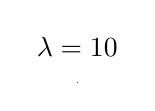
\begin{tikzpicture}[%
font=\footnotesize
]

\begin{axis}[%
width=0.951\figwidth,
height=\figheight,
at={(0\figwidth,0\figheight)},
scale only axis,
xmin=0,
xmax=3,
tick align=outside,
xlabel={Moneyness},
xmajorgrids,
ymin=0,
ymax=5,
ylabel={Remaining Time},
ymajorgrids,
zmin=0,
zmax=0.15,
zlabel={Relative Increase},
zmajorgrids,
view={50}{40},
axis background/.style={fill=white},
title style={font=\bfseries},
title={$\lambda = 10$},
axis x line*=bottom,
axis y line*=left,
axis z line*=left
]

\addplot3[%
surf,
shader=flat corner,draw=black,z buffer=sort,colormap={mymap}{[1pt] rgb(0pt)=(0.2081,0.1663,0.5292); rgb(1pt)=(0.211624,0.189781,0.577676); rgb(2pt)=(0.212252,0.213771,0.626971); rgb(3pt)=(0.2081,0.2386,0.677086); rgb(4pt)=(0.195905,0.264457,0.7279); rgb(5pt)=(0.170729,0.291938,0.779248); rgb(6pt)=(0.125271,0.324243,0.830271); rgb(7pt)=(0.0591333,0.359833,0.868333); rgb(8pt)=(0.0116952,0.38751,0.881957); rgb(9pt)=(0.00595714,0.408614,0.882843); rgb(10pt)=(0.0165143,0.4266,0.878633); rgb(11pt)=(0.0328524,0.443043,0.871957); rgb(12pt)=(0.0498143,0.458571,0.864057); rgb(13pt)=(0.0629333,0.47369,0.855438); rgb(14pt)=(0.0722667,0.488667,0.8467); rgb(15pt)=(0.0779429,0.503986,0.838371); rgb(16pt)=(0.0793476,0.520024,0.831181); rgb(17pt)=(0.0749429,0.537543,0.826271); rgb(18pt)=(0.0640571,0.556986,0.823957); rgb(19pt)=(0.0487714,0.577224,0.822829); rgb(20pt)=(0.0343429,0.596581,0.819852); rgb(21pt)=(0.0265,0.6137,0.8135); rgb(22pt)=(0.0238905,0.628662,0.803762); rgb(23pt)=(0.0230905,0.641786,0.791267); rgb(24pt)=(0.0227714,0.653486,0.776757); rgb(25pt)=(0.0266619,0.664195,0.760719); rgb(26pt)=(0.0383714,0.674271,0.743552); rgb(27pt)=(0.0589714,0.683757,0.725386); rgb(28pt)=(0.0843,0.692833,0.706167); rgb(29pt)=(0.113295,0.7015,0.685857); rgb(30pt)=(0.145271,0.709757,0.664629); rgb(31pt)=(0.180133,0.717657,0.642433); rgb(32pt)=(0.217829,0.725043,0.619262); rgb(33pt)=(0.258643,0.731714,0.595429); rgb(34pt)=(0.302171,0.737605,0.571186); rgb(35pt)=(0.348167,0.742433,0.547267); rgb(36pt)=(0.395257,0.7459,0.524443); rgb(37pt)=(0.44201,0.748081,0.503314); rgb(38pt)=(0.487124,0.749062,0.483976); rgb(39pt)=(0.530029,0.749114,0.466114); rgb(40pt)=(0.570857,0.748519,0.44939); rgb(41pt)=(0.609852,0.747314,0.433686); rgb(42pt)=(0.6473,0.7456,0.4188); rgb(43pt)=(0.683419,0.743476,0.404433); rgb(44pt)=(0.71841,0.741133,0.390476); rgb(45pt)=(0.752486,0.7384,0.376814); rgb(46pt)=(0.785843,0.735567,0.363271); rgb(47pt)=(0.818505,0.732733,0.34979); rgb(48pt)=(0.850657,0.7299,0.336029); rgb(49pt)=(0.882433,0.727433,0.3217); rgb(50pt)=(0.913933,0.725786,0.306276); rgb(51pt)=(0.944957,0.726114,0.288643); rgb(52pt)=(0.973895,0.731395,0.266648); rgb(53pt)=(0.993771,0.745457,0.240348); rgb(54pt)=(0.999043,0.765314,0.216414); rgb(55pt)=(0.995533,0.786057,0.196652); rgb(56pt)=(0.988,0.8066,0.179367); rgb(57pt)=(0.978857,0.827143,0.163314); rgb(58pt)=(0.9697,0.848138,0.147452); rgb(59pt)=(0.962586,0.870514,0.1309); rgb(60pt)=(0.958871,0.8949,0.113243); rgb(61pt)=(0.959824,0.921833,0.0948381); rgb(62pt)=(0.9661,0.951443,0.0755333); rgb(63pt)=(0.9763,0.9831,0.0538)},mesh/rows=25]
table[row sep=crcr, point meta=\thisrow{c}] {%
%
x	y	z	c\\
0	0.01	0.0197522420358995	0.0197522420358995\\
0	0.111836734693878	0.0600837014563599	0.0600837014563599\\
0	0.213673469387755	0.0761762577802557	0.0761762577802557\\
0	0.315510204081633	0.0855032448453112	0.0855032448453112\\
0	0.41734693877551	0.0913812033905288	0.0913812033905288\\
0	0.519183673469388	0.0952016788264122	0.0952016788264122\\
0	0.621020408163265	0.0976940959400998	0.0976940959400998\\
0	0.722857142857143	0.0992870953419485	0.0992870953419485\\
0	0.82469387755102	0.10025104770253	0.10025104770253\\
0	0.926530612244898	0.100765006012479	0.100765006012479\\
0	1.02836734693878	0.100951871968248	0.100951871968248\\
0	1.13020408163265	0.100898360599009	0.100898360599009\\
0	1.23204081632653	0.100667005808178	0.100667005808178\\
0	1.33387755102041	0.100303708133623	0.100303708133623\\
0	1.43571428571429	0.0998426516759935	0.0998426516759935\\
0	1.53755102040816	0.0993096020031434	0.0993096020031434\\
0	1.63938775510204	0.0987241728571005	0.0987241728571005\\
0	1.74122448979592	0.0981014168773813	0.0981014168773813\\
0	1.8430612244898	0.0974529621884803	0.0974529621884803\\
0	1.94489795918367	0.0967878373564366	0.0967878373564366\\
0	2.04673469387755	0.0961130785035642	0.0961130785035642\\
0	2.14857142857143	0.0954341816319018	0.0954341816319018\\
0	2.25040816326531	0.0947554433444925	0.0947554433444925\\
0	2.35224489795918	0.0940802200454415	0.0940802200454415\\
0	2.45408163265306	0.0934111268869391	0.0934111268869391\\
0	2.55591836734694	0.0927501917042342	0.0927501917042342\\
0	2.65775510204082	0.0920989749957982	0.0920989749957982\\
0	2.75959183673469	0.0914586640613929	0.0914586640613929\\
0	2.86142857142857	0.0908301473103855	0.0908301473103855\\
0	2.96326530612245	0.0902140732401826	0.0902140732401826\\
0	3.06510204081633	0.0896108974803048	0.0896108974803048\\
0	3.1669387755102	0.0890209204866583	0.0890209204866583\\
0	3.26877551020408	0.0884443178671263	0.0884443178671263\\
0	3.37061224489796	0.0878811648676017	0.0878811648676017\\
0	3.47244897959184	0.0873314562072941	0.0873314562072941\\
0	3.57428571428571	0.0867951221923056	0.0867951221923056\\
0	3.67612244897959	0.0862720418378935	0.0862720418378935\\
0	3.77795918367347	0.0857620535767664	0.0857620535767664\\
0	3.87979591836735	0.0852649640123671	0.0852649640123671\\
0	3.98163265306122	0.0847805550827845	0.0847805550827845\\
0	4.0834693877551	0.0843085899291417	0.0843085899291417\\
0	4.18530612244898	0.0838488177041784	0.0838488177041784\\
0	4.28714285714286	0.0834009775124139	0.0834009775124139\\
0	4.38897959183674	0.0829648016361722	0.0829648016361722\\
0	4.49081632653061	0.0825400181735804	0.0825400181735804\\
0	4.59265306122449	0.0821263531916695	0.0821263531916695\\
0	4.69448979591837	0.0817235324781751	0.0817235324781751\\
0	4.79632653061224	0.0813312829615459	0.0813312829615459\\
0	4.89816326530612	0.0809493338561255	0.0809493338561255\\
0	5	0.0805774175790751	0.0805774175790751\\
0.125	0.01	9.92179509835551e-05	9.92179509835551e-05\\
0.125	0.111836734693878	0.0198265057212913	0.0198265057212913\\
0.125	0.213673469387755	0.0353860342074051	0.0353860342074051\\
0.125	0.315510204081633	0.046083841619548	0.046083841619548\\
0.125	0.41734693877551	0.0537382029081841	0.0537382029081841\\
0.125	0.519183673469388	0.0593709691119292	0.0593709691119292\\
0.125	0.621020408163265	0.0635947267628623	0.0635947267628623\\
0.125	0.722857142857143	0.0668012612724884	0.0668012612724884\\
0.125	0.82469387755102	0.0692536400371075	0.0692536400371075\\
0.125	0.926530612244898	0.0711351700328877	0.0711351700328877\\
0.125	1.02836734693878	0.072577355204533	0.072577355204533\\
0.125	1.13020408163265	0.0736767851215599	0.0736767851215599\\
0.125	1.23204081632653	0.0745058025195642	0.0745058025195642\\
0.125	1.33387755102041	0.0751194892550008	0.0751194892550008\\
0.125	1.43571428571429	0.075560380037001	0.075560380037001\\
0.125	1.53755102040816	0.075861724080756	0.075861724080756\\
0.125	1.63938775510204	0.076049791164193	0.076049791164193\\
0.125	1.74122448979592	0.0761455328278358	0.0761455328278358\\
0.125	1.8430612244898	0.076165798837437	0.076165798837437\\
0.125	1.94489795918367	0.0761242410177393	0.0761242410177393\\
0.125	2.04673469387755	0.0760319935803993	0.0760319935803993\\
0.125	2.14857142857143	0.0758981912350715	0.0758981912350715\\
0.125	2.25040816326531	0.0757303679591027	0.0757303679591027\\
0.125	2.35224489795918	0.0755347592007689	0.0755347592007689\\
0.125	2.45408163265306	0.0753165832456871	0.0753165832456871\\
0.125	2.55591836734694	0.0750801563887431	0.0750801563887431\\
0.125	2.65775510204082	0.0748291226664346	0.0748291226664346\\
0.125	2.75959183673469	0.0745665380206086	0.0745665380206086\\
0.125	2.86142857142857	0.0742949768963602	0.0742949768963602\\
0.125	2.96326530612245	0.0740166125318559	0.0740166125318559\\
0.125	3.06510204081633	0.0737332823951365	0.0737332823951365\\
0.125	3.1669387755102	0.0734465423458686	0.0734465423458686\\
0.125	3.26877551020408	0.0731577103752346	0.0731577103752346\\
0.125	3.37061224489796	0.0728679036952889	0.0728679036952889\\
0.125	3.47244897959184	0.0725780691791715	0.0725780691791715\\
0.125	3.57428571428571	0.0722890088551212	0.0722890088551212\\
0.125	3.67612244897959	0.0720014012743902	0.0720014012743902\\
0.125	3.77795918367347	0.0717158194841871	0.0717158194841871\\
0.125	3.87979591836735	0.0714327461953842	0.0714327461953842\\
0.125	3.98163265306122	0.0711525866229807	0.0711525866229807\\
0.125	4.0834693877551	0.0708756793885292	0.0708756793885292\\
0.125	4.18530612244898	0.0706023058028211	0.0706023058028211\\
0.125	4.28714285714286	0.0703326977902152	0.0703326977902152\\
0.125	4.38897959183674	0.0700670446701093	0.0700670446701093\\
0.125	4.49081632653061	0.0698054989738887	0.0698054989738887\\
0.125	4.59265306122449	0.0695481811974029	0.0695481811974029\\
0.125	4.69448979591837	0.0692951851677726	0.0692951851677726\\
0.125	4.79632653061224	0.0690465800889358	0.0690465800889358\\
0.125	4.89816326530612	0.0688024149130329	0.0688024149130329\\
0.125	5	0.0685627207143826	0.0685627207143826\\
0.25	0.01	2.64664767695518e-09	2.64664767695518e-09\\
0.25	0.111836734693878	0.00445898441696202	0.00445898441696202\\
0.25	0.213673469387755	0.0135638115712497	0.0135638115712497\\
0.25	0.315510204081633	0.0218708979085776	0.0218708979085776\\
0.25	0.41734693877551	0.0287456858083525	0.0287456858083525\\
0.25	0.519183673469388	0.0343408939011759	0.0343408939011759\\
0.25	0.621020408163265	0.0388951117115532	0.0388951117115532\\
0.25	0.722857142857143	0.0426183375037157	0.0426183375037157\\
0.25	0.82469387755102	0.0456781908576849	0.0456781908576849\\
0.25	0.926530612244898	0.0482053537024964	0.0482053537024964\\
0.25	1.02836734693878	0.0503014842540524	0.0503014842540524\\
0.25	1.13020408163265	0.0520460739235307	0.0520460739235307\\
0.25	1.23204081632653	0.0535017693947277	0.0535017693947277\\
0.25	1.33387755102041	0.0547183690242781	0.0547183690242781\\
0.25	1.43571428571429	0.0557357999923282	0.0557357999923282\\
0.25	1.53755102040816	0.0565863406165457	0.0565863406165457\\
0.25	1.63938775510204	0.0572962896560777	0.0572962896560777\\
0.25	1.74122448979592	0.0578872303877531	0.0578872303877531\\
0.25	1.8430612244898	0.0583769962107753	0.0583769962107753\\
0.25	1.94489795918367	0.0587804147840124	0.0587804147840124\\
0.25	2.04673469387755	0.0591098864118126	0.0591098864118126\\
0.25	2.14857142857143	0.0593758373608589	0.0593758373608589\\
0.25	2.25040816326531	0.059587077958642	0.059587077958642\\
0.25	2.35224489795918	0.0597510875634073	0.0597510875634073\\
0.25	2.45408163265306	0.0598742429534345	0.0598742429534345\\
0.25	2.55591836734694	0.0599620025881979	0.0599620025881979\\
0.25	2.65775510204082	0.0600190562133271	0.0600190562133271\\
0.25	2.75959183673469	0.0600494469232274	0.0600494469232274\\
0.25	2.86142857142857	0.060056671425227	0.060056671425227\\
0.25	2.96326530612245	0.0600437633037057	0.0600437633037057\\
0.25	3.06510204081633	0.060013361041243	0.060013361041243\\
0.25	3.1669387755102	0.0599677656690957	0.0599677656690957\\
0.25	3.26877551020408	0.059908988608064	0.059908988608064\\
0.25	3.37061224489796	0.0598387919633152	0.0598387919633152\\
0.25	3.47244897959184	0.0597587225359226	0.0597587225359226\\
0.25	3.57428571428571	0.0596701406398268	0.0596701406398268\\
0.25	3.67612244897959	0.059574244605647	0.059574244605647\\
0.25	3.77795918367347	0.0594720916884022	0.0594720916884022\\
0.25	3.87979591836735	0.0593646159651816	0.0593646159651816\\
0.25	3.98163265306122	0.0592526437038266	0.0592526437038266\\
0.25	4.0834693877551	0.0591369065991754	0.0591369065991754\\
0.25	4.18530612244898	0.0590180532050778	0.0590180532050778\\
0.25	4.28714285714286	0.0588966588348578	0.0588966588348578\\
0.25	4.38897959183674	0.0587732341576129	0.0587732341576129\\
0.25	4.49081632653061	0.0586482326806331	0.0586482326806331\\
0.25	4.59265306122449	0.0585220572777181	0.0585220572777181\\
0.25	4.69448979591837	0.0583950658979882	0.0583950658979882\\
0.25	4.79632653061224	0.0582675763464649	0.0582675763464649\\
0.25	4.89816326530612	0.0581398717900604	0.0581398717900604\\
0.25	5	0.0580122023992054	0.0580122023992054\\
0.375	0.01	2.03722767489391e-16	2.03722767489391e-16\\
0.375	0.111836734693878	0.000650617191335985	0.000650617191335985\\
0.375	0.213673469387755	0.00419963605935132	0.00419963605935132\\
0.375	0.315510204081633	0.00902511202310685	0.00902511202310685\\
0.375	0.41734693877551	0.0138669854312102	0.0138669854312102\\
0.375	0.519183673469388	0.0183056114483059	0.0183056114483059\\
0.375	0.621020408163265	0.0222394385458033	0.0222394385458033\\
0.375	0.722857142857143	0.0256785737357722	0.0256785737357722\\
0.375	0.82469387755102	0.0286695808981238	0.0286695808981238\\
0.375	0.926530612244898	0.0312674005771342	0.0312674005771342\\
0.375	1.02836734693878	0.0335249339464197	0.0335249339464197\\
0.375	1.13020408163265	0.0354895427661367	0.0354895427661367\\
0.375	1.23204081632653	0.0372023027104636	0.0372023027104636\\
0.375	1.33387755102041	0.0386983213812454	0.0386983213812454\\
0.375	1.43571428571429	0.0400074179985189	0.0400074179985189\\
0.375	1.53755102040816	0.0411548726065963	0.0411548726065963\\
0.375	1.63938775510204	0.0421621289912609	0.0421621289912609\\
0.375	1.74122448979592	0.0430474120283766	0.0430474120283766\\
0.375	1.8430612244898	0.0438262528938474	0.0438262528938474\\
0.375	1.94489795918367	0.0445119287152326	0.0445119287152326\\
0.375	2.04673469387755	0.045115827662162	0.045115827662162\\
0.375	2.14857142857143	0.0456477510855402	0.0456477510855402\\
0.375	2.25040816326531	0.0461161633876902	0.0461161633876902\\
0.375	2.35224489795918	0.0465283988685086	0.0465283988685086\\
0.375	2.45408163265306	0.0468908333013956	0.0468908333013956\\
0.375	2.55591836734694	0.0472090266319913	0.0472090266319913\\
0.375	2.65775510204082	0.047487842022385	0.047487842022385\\
0.375	2.75959183673469	0.0477315454876517	0.0477315454876517\\
0.375	2.86142857142857	0.0479438895719248	0.0479438895719248\\
0.375	2.96326530612245	0.0481281838622303	0.0481281838622303\\
0.375	3.06510204081633	0.0482873546142739	0.0482873546142739\\
0.375	3.1669387755102	0.0484239953421846	0.0484239953421846\\
0.375	3.26877551020408	0.0485404098842088	0.0485404098842088\\
0.375	3.37061224489796	0.0486386491822857	0.0486386491822857\\
0.375	3.47244897959184	0.0487205427921613	0.0487205427921613\\
0.375	3.57428571428571	0.0487877259616378	0.0487877259616378\\
0.375	3.67612244897959	0.0488416629692793	0.0488416629692793\\
0.375	3.77795918367347	0.0488836672976893	0.0488836672976893\\
0.375	3.87979591836735	0.0489149191190023	0.0489149191190023\\
0.375	3.98163265306122	0.0489364804912537	0.0489364804912537\\
0.375	4.0834693877551	0.0489493085994271	0.0489493085994271\\
0.375	4.18530612244898	0.0489542673215375	0.0489542673215375\\
0.375	4.28714285714286	0.0489521373586325	0.0489521373586325\\
0.375	4.38897959183674	0.0489436251183082	0.0489436251183082\\
0.375	4.49081632653061	0.04892937053098	0.04892937053098\\
0.375	4.59265306122449	0.0489099539476727	0.0489099539476727\\
0.375	4.69448979591837	0.0488859022252564	0.0488859022252564\\
0.375	4.79632653061224	0.0488576941149463	0.0488576941149463\\
0.375	4.89816326530612	0.0488257650411478	0.0488257650411478\\
0.375	5	0.0487905113476064	0.0487905113476064\\
0.5	0.01	3.70028753662104e-26	3.70028753662104e-26\\
0.5	0.111836734693878	5.94946989417277e-05	5.94946989417277e-05\\
0.5	0.213673469387755	0.00103286130605644	0.00103286130605644\\
0.5	0.315510204081633	0.00320457292130833	0.00320457292130833\\
0.5	0.41734693877551	0.00598854649992047	0.00598854649992047\\
0.5	0.519183673469388	0.00894298482321773	0.00894298482321773\\
0.5	0.621020408163265	0.0118358208987035	0.0118358208987035\\
0.5	0.722857142857143	0.0145593720500607	0.0145593720500607\\
0.5	0.82469387755102	0.0170711664335375	0.0170711664335375\\
0.5	0.926530612244898	0.0193617027981503	0.0193617027981503\\
0.5	1.02836734693878	0.021437607475451	0.021437607475451\\
0.5	1.13020408163265	0.0233128770689363	0.0233128770689363\\
0.5	1.23204081632653	0.0250043311434896	0.0250043311434896\\
0.5	1.33387755102041	0.0265292771455933	0.0265292771455933\\
0.5	1.43571428571429	0.0279043504824345	0.0279043504824345\\
0.5	1.53755102040816	0.0291449827472679	0.0291449827472679\\
0.5	1.63938775510204	0.0302652048034932	0.0302652048034932\\
0.5	1.74122448979592	0.0312776253685543	0.0312776253685543\\
0.5	1.8430612244898	0.0321934977881601	0.0321934977881601\\
0.5	1.94489795918367	0.033022827100663	0.033022827100663\\
0.5	2.04673469387755	0.0337744913326435	0.0337744913326435\\
0.5	2.14857142857143	0.0344563631789447	0.0344563631789447\\
0.5	2.25040816326531	0.0350754250726053	0.0350754250726053\\
0.5	2.35224489795918	0.0356378744815538	0.0356378744815538\\
0.5	2.45408163265306	0.0361492183827138	0.0361492183827138\\
0.5	2.55591836734694	0.0366143569967371	0.0366143569967371\\
0.5	2.65775510204082	0.0370376574388631	0.0370376574388631\\
0.5	2.75959183673469	0.0374230181961292	0.0374230181961292\\
0.5	2.86142857142857	0.0377739254190145	0.0377739254190145\\
0.5	2.96326530612245	0.0380935019982981	0.0380935019982981\\
0.5	3.06510204081633	0.0383845503326754	0.0383845503326754\\
0.5	3.1669387755102	0.0386495896065605	0.0386495896065605\\
0.5	3.26877551020408	0.0388908883056508	0.0388908883056508\\
0.5	3.37061224489796	0.0391104926084133	0.0391104926084133\\
0.5	3.47244897959184	0.0393102512087515	0.0393102512087515\\
0.5	3.57428571428571	0.0394918370504603	0.0394918370504603\\
0.5	3.67612244897959	0.0396567663880927	0.0396567663880927\\
0.5	3.77795918367347	0.0398064155312333	0.0398064155312333\\
0.5	3.87979591836735	0.0399420355792589	0.0399420355792589\\
0.5	3.98163265306122	0.0400647654106559	0.0400647654106559\\
0.5	4.0834693877551	0.0401756431540404	0.0401756431540404\\
0.5	4.18530612244898	0.0402756163363929	0.0402756163363929\\
0.5	4.28714285714286	0.0403655508769465	0.0403655508769465\\
0.5	4.38897959183674	0.0404462390720211	0.0404462390720211\\
0.5	4.49081632653061	0.0405184066962868	0.0405184066962868\\
0.5	4.59265306122449	0.0405827193289987	0.0405827193289987\\
0.5	4.69448979591837	0.0406397879992264	0.0406397879992264\\
0.5	4.79632653061224	0.040690174231665	0.040690174231665\\
0.5	4.89816326530612	0.040734394563928	0.040734394563928\\
0.5	5	0.0407729245970507	0.0407729245970507\\
0.625	0.01	1.45990234661222e-38	1.45990234661222e-38\\
0.625	0.111836734693878	3.32923318666829e-06	3.32923318666829e-06\\
0.625	0.213673469387755	0.000199194162623941	0.000199194162623941\\
0.625	0.315510204081633	0.000970826009717587	0.000970826009717587\\
0.625	0.41734693877551	0.00230101976756561	0.00230101976756561\\
0.625	0.519183673469388	0.0039851525281445	0.0039851525281445\\
0.625	0.621020408163265	0.00584062892391577	0.00584062892391577\\
0.625	0.722857142857143	0.00774346265338258	0.00774346265338258\\
0.625	0.82469387755102	0.00961757418340774	0.00961757418340774\\
0.625	0.926530612244898	0.0114193034129716	0.0114193034129716\\
0.625	1.02836734693878	0.0131255779883584	0.0131255779883584\\
0.625	1.13020408163265	0.0147260257534727	0.0147260257534727\\
0.625	1.23204081632653	0.016217948924155	0.016217948924155\\
0.625	1.33387755102041	0.017603174067106	0.017603174067106\\
0.625	1.43571428571429	0.0188860907724042	0.0188860907724042\\
0.625	1.53755102040816	0.0200724359244235	0.0200724359244235\\
0.625	1.63938775510204	0.021168545136083	0.021168545136083\\
0.625	1.74122448979592	0.0221808975054771	0.0221808975054771\\
0.625	1.8430612244898	0.0231158449736374	0.0231158449736374\\
0.625	1.94489795918367	0.0239794579489778	0.0239794579489778\\
0.625	2.04673469387755	0.0247774439942793	0.0247774439942793\\
0.625	2.14857142857143	0.0255151121100597	0.0255151121100597\\
0.625	2.25040816326531	0.0261973650790262	0.0261973650790262\\
0.625	2.35224489795918	0.0268287086506774	0.0268287086506774\\
0.625	2.45408163265306	0.0274132703882457	0.0274132703882457\\
0.625	2.55591836734694	0.0279548236045045	0.0279548236045045\\
0.625	2.65775510204082	0.0284568134981968	0.0284568134981968\\
0.625	2.75959183673469	0.028922383696422	0.028922383696422\\
0.625	2.86142857142857	0.029354402118411	0.029354402118411\\
0.625	2.96326530612245	0.0297554855362342	0.0297554855362342\\
0.625	3.06510204081633	0.030128022504413	0.030128022504413\\
0.625	3.1669387755102	0.0304741945193239	0.0304741945193239\\
0.625	3.26877551020408	0.0307959953875174	0.0307959953875174\\
0.625	3.37061224489796	0.0310952488538614	0.0310952488538614\\
0.625	3.47244897959184	0.0313736245818143	0.0313736245818143\\
0.625	3.57428571428571	0.0316326525997766	0.0316326525997766\\
0.625	3.67612244897959	0.0318737363364354	0.0318737363364354\\
0.625	3.77795918367347	0.0320981643690134	0.0320981643690134\\
0.625	3.87979591836735	0.0323071210044703	0.0323071210044703\\
0.625	3.98163265306122	0.0325016958070421	0.0325016958070421\\
0.625	4.0834693877551	0.0326828921773906	0.0326828921773906\\
0.625	4.18530612244898	0.0328516350799274	0.0328516350799274\\
0.625	4.28714285714286	0.0330087780061407	0.0330087780061407\\
0.625	4.38897959183674	0.0331551092533008	0.0331551092533008\\
0.625	4.49081632653061	0.0332913575899675	0.0332913575899675\\
0.625	4.59265306122449	0.0334181973723463	0.0334181973723463\\
0.625	4.69448979591837	0.033536253168799	0.033536253168799\\
0.625	4.79632653061224	0.033646103943693	0.033646103943693\\
0.625	4.89816326530612	0.0337482868462597	0.0337482868462597\\
0.625	5	0.0338433006451848	0.0338433006451848\\
0.75	0.01	1.20100339712943e-53	1.20100339712943e-53\\
0.75	0.111836734693878	1.12143506265015e-07	1.12143506265015e-07\\
0.75	0.213673469387755	2.98297908358975e-05	2.98297908358975e-05\\
0.75	0.315510204081633	0.000249239261949281	0.000249239261949281\\
0.75	0.41734693877551	0.000782649654649953	0.000782649654649953\\
0.75	0.519183673469388	0.00161334138969473	0.00161334138969473\\
0.75	0.621020408163265	0.00266366542964936	0.00266366542964936\\
0.75	0.722857142857143	0.00385255608298017	0.00385255608298017\\
0.75	0.82469387755102	0.00511445688752638	0.00511445688752638\\
0.75	0.926530612244898	0.00640151686034207	0.00640151686034207\\
0.75	1.02836734693878	0.00768071247088823	0.00768071247088823\\
0.75	1.13020408163265	0.00893019348015692	0.00893019348015692\\
0.75	1.23204081632653	0.0101361366641128	0.0101361366641128\\
0.75	1.33387755102041	0.0112903399760652	0.0112903399760652\\
0.75	1.43571428571429	0.0123884729104885	0.0123884729104885\\
0.75	1.53755102040816	0.0134288340986904	0.0134288340986904\\
0.75	1.63938775510204	0.0144114796909907	0.0144114796909907\\
0.75	1.74122448979592	0.0153376159221666	0.0153376159221666\\
0.75	1.8430612244898	0.0162091776748847	0.0162091776748847\\
0.75	1.94489795918367	0.0170285373252146	0.0170285373252146\\
0.75	2.04673469387755	0.0177983046878008	0.0177983046878008\\
0.75	2.14857142857143	0.0185211906527903	0.0185211906527903\\
0.75	2.25040816326531	0.01919991536551	0.01919991536551\\
0.75	2.35224489795918	0.0198371475562988	0.0198371475562988\\
0.75	2.45408163265306	0.0204354656340461	0.0204354656340461\\
0.75	2.55591836734694	0.0209973339483287	0.0209973339483287\\
0.75	2.65775510204082	0.021525089575108	0.021525089575108\\
0.75	2.75959183673469	0.0220209363479518	0.0220209363479518\\
0.75	2.86142857142857	0.0224869438185363	0.0224869438185363\\
0.75	2.96326530612245	0.02292504950937	0.02292504950937\\
0.75	3.06510204081633	0.0233370633029229	0.0233370633029229\\
0.75	3.1669387755102	0.0237246731533574	0.0237246731533574\\
0.75	3.26877551020408	0.0240894515506931	0.0240894515506931\\
0.75	3.37061224489796	0.0244328623410953	0.0244328623410953\\
0.75	3.47244897959184	0.0247562676311295	0.0247562676311295\\
0.75	3.57428571428571	0.0250609345924624	0.0250609345924624\\
0.75	3.67612244897959	0.0253480420466656	0.0253480420466656\\
0.75	3.77795918367347	0.025618686754664	0.025618686754664\\
0.75	3.87979591836735	0.0258738893670851	0.0258738893670851\\
0.75	3.98163265306122	0.0261146000139923	0.0261146000139923\\
0.75	4.0834693877551	0.0263417035278724	0.0263417035278724\\
0.75	4.18530612244898	0.0265560243042101	0.0265560243042101\\
0.75	4.28714285714286	0.0267583308109061	0.0267583308109061\\
0.75	4.38897959183674	0.0269493397621874	0.0269493397621874\\
0.75	4.49081632653061	0.0271297199752429	0.0271297199752429\\
0.75	4.59265306122449	0.0273000959291387	0.0273000959291387\\
0.75	4.69448979591837	0.0274610510459884	0.0274610510459884\\
0.75	4.79632653061224	0.0276131307141825	0.0276131307141825\\
0.75	4.89816326530612	0.0277568450728886	0.0277568450728886\\
0.75	5	0.0278926715761978	0.0278926715761978\\
0.875	0.01	2.01341581267473e-71	2.01341581267473e-71\\
0.875	0.111836734693878	2.24776740382203e-09	2.24776740382203e-09\\
0.875	0.213673469387755	3.44278494061858e-06	3.44278494061858e-06\\
0.875	0.315510204081633	5.3931007105441e-05	5.3931007105441e-05\\
0.875	0.41734693877551	0.000234661241053618	0.000234661241053618\\
0.875	0.519183673469388	0.0005913679675254	0.0005913679675254\\
0.875	0.621020408163265	0.00111953437471336	0.00111953437471336\\
0.875	0.722857142857143	0.00178873055954319	0.00178873055954319\\
0.875	0.82469387755102	0.00256191629403851	0.00256191629403851\\
0.875	0.926530612244898	0.0034047244146717	0.0034047244146717\\
0.875	1.02836734693878	0.00428865631106325	0.00428865631106325\\
0.875	1.13020408163265	0.00519144966185709	0.00519144966185709\\
0.875	1.23204081632653	0.00609636001712223	0.00609636001712223\\
0.875	1.33387755102041	0.00699115282877997	0.00699115282877997\\
0.875	1.43571428571429	0.0078671300591245	0.0078671300591245\\
0.875	1.53755102040816	0.00871830062322136	0.00871830062322136\\
0.875	1.63938775510204	0.00954071329086731	0.00954071329086731\\
0.875	1.74122448979592	0.0103319364973015	0.0103319364973015\\
0.875	1.8430612244898	0.0110906597436705	0.0110906597436705\\
0.875	1.94489795918367	0.0118163913258461	0.0118163913258461\\
0.875	2.04673469387755	0.0125092305927675	0.0125092305927675\\
0.875	2.14857142857143	0.0131696971062627	0.0131696971062627\\
0.875	2.25040816326531	0.0137986029194064	0.0137986029194064\\
0.875	2.35224489795918	0.0143969573953695	0.0143969573953695\\
0.875	2.45408163265306	0.0149658965322291	0.0149658965322291\\
0.875	2.55591836734694	0.0155066307251591	0.0155066307251591\\
0.875	2.65775510204082	0.0160204063946358	0.0160204063946358\\
0.875	2.75959183673469	0.0165084780402029	0.0165084780402029\\
0.875	2.86142857142857	0.0169720881299586	0.0169720881299586\\
0.875	2.96326530612245	0.0174124528746191	0.0174124528746191\\
0.875	3.06510204081633	0.017830752414485	0.017830752414485\\
0.875	3.1669387755102	0.0182281243079099	0.0182281243079099\\
0.875	3.26877551020408	0.0186056594809536	0.0186056594809536\\
0.875	3.37061224489796	0.0189644000022709	0.0189644000022709\\
0.875	3.47244897959184	0.0193053382016589	0.0193053382016589\\
0.875	3.57428571428571	0.0196294167675384	0.0196294167675384\\
0.875	3.67612244897959	0.0199375295472669	0.0199375295472669\\
0.875	3.77795918367347	0.0202305228415263	0.0202305228415263\\
0.875	3.87979591836735	0.0205091970352794	0.0205091970352794\\
0.875	3.98163265306122	0.0207743084468448	0.0207743084468448\\
0.875	4.0834693877551	0.0210265713064412	0.0210265713064412\\
0.875	4.18530612244898	0.0212666597982885	0.0212666597982885\\
0.875	4.28714285714286	0.0214952101177147	0.0214952101177147\\
0.875	4.38897959183674	0.0217128225079598	0.0217128225079598\\
0.875	4.49081632653061	0.0219200632514578	0.0219200632514578\\
0.875	4.59265306122449	0.022117466598051	0.022117466598051\\
0.875	4.69448979591837	0.0223055366184054	0.0223055366184054\\
0.875	4.79632653061224	0.0224847489752841	0.0224847489752841\\
0.875	4.89816326530612	0.0226555526086283	0.0226555526086283\\
0.875	5	0.0228183713328401	0.0228183713328401\\
1	0.01	6.78224000215881e-92	6.78224000215881e-92\\
1	0.111836734693878	2.65877542812556e-11	2.65877542812556e-11\\
1	0.213673469387755	3.04480269838768e-07	3.04480269838768e-07\\
1	0.315510204081633	9.79316406494778e-06	9.79316406494778e-06\\
1	0.41734693877551	6.18080142400418e-05	6.18080142400418e-05\\
1	0.519183673469388	0.000195707341481308	0.000195707341481308\\
1	0.621020408163265	0.000432605609259186	0.000432605609259186\\
1	0.722857142857143	0.000773439904863789	0.000773439904863789\\
1	0.82469387755102	0.00120663866951148	0.00120663866951148\\
1	0.926530612244898	0.00171530490985691	0.00171530490985691\\
1	1.02836734693878	0.00228167826747265	0.00228167826747265\\
1	1.13020408163265	0.00288938396561992	0.00288938396561992\\
1	1.23204081632653	0.00352433026864215	0.00352433026864215\\
1	1.33387755102041	0.00417488719963103	0.00417488719963103\\
1	1.43571428571429	0.0048317256866841	0.0048317256866841\\
1	1.53755102040816	0.00548752315907224	0.00548752315907224\\
1	1.63938775510204	0.00613663962011749	0.00613663962011749\\
1	1.74122448979592	0.00677481231467791	0.00677481231467791\\
1	1.8430612244898	0.00739888794716575	0.00739888794716575\\
1	1.94489795918367	0.00800659694970637	0.00800659694970637\\
1	2.04673469387755	0.00859636764918387	0.00859636764918387\\
1	2.14857142857143	0.00916717554231399	0.00916717554231399\\
1	2.25040816326531	0.00971842222592956	0.00971842222592956\\
1	2.35224489795918	0.0102498387785019	0.0102498387785019\\
1	2.45408163265306	0.0107614090026693	0.0107614090026693\\
1	2.55591836734694	0.0112533086480418	0.0112533086480418\\
1	2.65775510204082	0.011725857414362	0.011725857414362\\
1	2.75959183673469	0.0121794811368762	0.0121794811368762\\
1	2.86142857142857	0.0126146820647662	0.0126146820647662\\
1	2.96326530612245	0.0130320155629903	0.0130320155629903\\
1	3.06510204081633	0.0134320719081211	0.0134320719081211\\
1	3.1669387755102	0.0138154621219388	0.0138154621219388\\
1	3.26877551020408	0.0141828070044704	0.0141828070044704\\
1	3.37061224489796	0.0145347287013568	0.0145347287013568\\
1	3.47244897959184	0.0148718442777602	0.0148718442777602\\
1	3.57428571428571	0.0151947608798084	0.0151947608798084\\
1	3.67612244897959	0.0155040721507256	0.0155040721507256\\
1	3.77795918367347	0.0158003556370534	0.0158003556370534\\
1	3.87979591836735	0.0160841709744758	0.0160841709744758\\
1	3.98163265306122	0.0163560586857105	0.0163560586857105\\
1	4.0834693877551	0.0166165394570445	0.0166165394570445\\
1	4.18530612244898	0.0168661137872406	0.0168661137872406\\
1	4.28714285714286	0.0171052619241568	0.0171052619241568\\
1	4.38897959183674	0.0173344440216668	0.0173344440216668\\
1	4.49081632653061	0.0175541004632361	0.0175541004632361\\
1	4.59265306122449	0.0177646523095106	0.0177646523095106\\
1	4.69448979591837	0.017966501836083	0.017966501836083\\
1	4.79632653061224	0.018160033134647	0.018160033134647\\
1	4.89816326530612	0.0183456127564018	0.0183456127564018\\
1	5	0.0185235903810931	0.0185235903810931\\
1.125	0.01	4.54827593314771e-115	4.54827593314771e-115\\
1.125	0.111836734693878	1.84472775438902e-13	1.84472775438902e-13\\
1.125	0.213673469387755	2.05429951333657e-08	2.05429951333657e-08\\
1.125	0.315510204081633	1.48715714842033e-06	1.48715714842033e-06\\
1.125	0.41734693877551	1.42608332276917e-05	1.42608332276917e-05\\
1.125	0.519183673469388	5.83365125023247e-05	5.83365125023247e-05\\
1.125	0.621020408163265	0.000153376185599684	0.000153376185599684\\
1.125	0.722857142857143	0.000310900759801502	0.000310900759801502\\
1.125	0.82469387755102	0.000533524247525586	0.000533524247525586\\
1.125	0.926530612244898	0.00081743128254612	0.00081743128254612\\
1.125	1.02836734693878	0.00115518315046633	0.00115518315046633\\
1.125	1.13020408163265	0.00153783675281948	0.00153783675281948\\
1.125	1.23204081632653	0.0019562840732015	0.0019562840732015\\
1.125	1.33387755102041	0.00240199527157429	0.00240199527157429\\
1.125	1.43571428571429	0.00286736984686856	0.00286736984686856\\
1.125	1.53755102040816	0.0033458525000504	0.0033458525000504\\
1.125	1.63938775510204	0.00383191829098274	0.00383191829098274\\
1.125	1.74122448979592	0.00432099196844777	0.00432099196844777\\
1.125	1.8430612244898	0.00480933966473643	0.00480933966473643\\
1.125	1.94489795918367	0.00529395433376361	0.00529395433376361\\
1.125	2.04673469387755	0.00577244614598387	0.00577244614598387\\
1.125	2.14857142857143	0.00624294310613915	0.00624294310613915\\
1.125	2.25040816326531	0.00670400379835722	0.00670400379835722\\
1.125	2.35224489795918	0.00715454234782248	0.00715454234782248\\
1.125	2.45408163265306	0.00759376477747688	0.00759376477747688\\
1.125	2.55591836734694	0.0080211155437763	0.0080211155437763\\
1.125	2.65775510204082	0.00843623292622558	0.00843623292622558\\
1.125	2.75959183673469	0.00883891198561537	0.00883891198561537\\
1.125	2.86142857142857	0.00922907391743379	0.00922907391743379\\
1.125	2.96326530612245	0.0096067407658939	0.0096067407658939\\
1.125	3.06510204081633	0.00997201460662641	0.00997201460662641\\
1.125	3.1669387755102	0.0103250604402742	0.0103250604402742\\
1.125	3.26877551020408	0.0106660921596107	0.0106660921596107\\
1.125	3.37061224489796	0.0109953610577132	0.0109953610577132\\
1.125	3.47244897959184	0.0113131464344402	0.0113131464344402\\
1.125	3.57428571428571	0.0116197479342262	0.0116197479342262\\
1.125	3.67612244897959	0.0119154793116372	0.0119154793116372\\
1.125	3.77795918367347	0.0122006633739221	0.0122006633739221\\
1.125	3.87979591836735	0.0124756278935585	0.0124756278935585\\
1.125	3.98163265306122	0.0127407023199635	0.0127407023199635\\
1.125	4.0834693877551	0.0129962151493995	0.0129962151493995\\
1.125	4.18530612244898	0.0132424918367196	0.0132424918367196\\
1.125	4.28714285714286	0.0134798531528817	0.0134798531528817\\
1.125	4.38897959183674	0.0137086139088788	0.0137086139088788\\
1.125	4.49081632653061	0.0139290819805105	0.0139290819805105\\
1.125	4.59265306122449	0.0141415575797866	0.0141415575797866\\
1.125	4.69448979591837	0.0143463327281252	0.0143463327281252\\
1.125	4.79632653061224	0.0145436908942562	0.0145436908942562\\
1.125	4.89816326530612	0.0147339067661362	0.0147339067661362\\
1.125	5	0.0149172461314732	0.0149172461314732\\
1.25	0.01	6.03364656930728e-141	6.03364656930728e-141\\
1.25	0.111836734693878	7.47365404844728e-16	7.47365404844728e-16\\
1.25	0.213673469387755	1.05367940105581e-09	1.05367940105581e-09\\
1.25	0.315510204081633	1.8832929757275e-07	1.8832929757275e-07\\
1.25	0.41734693877551	2.87556745602598e-06	2.87556745602598e-06\\
1.25	0.519183673469388	1.56310938023734e-05	1.56310938023734e-05\\
1.25	0.621020408163265	4.9805858178158e-05	4.9805858178158e-05\\
1.25	0.722857142857143	0.000116002072547181	0.000116002072547181\\
1.25	0.82469387755102	0.000221158101554387	0.000221158101554387\\
1.25	0.926530612244898	0.000368025392433472	0.000368025392433472\\
1.25	1.02836734693878	0.000555937012250459	0.000555937012250459\\
1.25	1.13020408163265	0.000781915580470204	0.000781915580470204\\
1.25	1.23204081632653	0.0010416648419256	0.0010416648419256\\
1.25	1.33387755102041	0.00133030949013908	0.00133030949013908\\
1.25	1.43571428571429	0.00164289039144179	0.00164289039144179\\
1.25	1.53755102040816	0.0019746675202868	0.0019746675202868\\
1.25	1.63938775510204	0.00232128656523788	0.00232128656523788\\
1.25	1.74122448979592	0.00267885508562717	0.00267885508562717\\
1.25	1.8430612244898	0.0030439618455241	0.0030439618455241\\
1.25	1.94489795918367	0.00341366247232557	0.00341366247232557\\
1.25	2.04673469387755	0.00378544670886697	0.00378544670886697\\
1.25	2.14857142857143	0.00415719698241682	0.00415719698241682\\
1.25	2.25040816326531	0.00452714426387439	0.00452714426387439\\
1.25	2.35224489795918	0.00489382472545804	0.00489382472545804\\
1.25	2.45408163265306	0.00525603912259968	0.00525603912259968\\
1.25	2.55591836734694	0.00561281583333084	0.00561281583333084\\
1.25	2.65775510204082	0.00596337788314651	0.00596337788314651\\
1.25	2.75959183673469	0.00630711392792691	0.00630711392792691\\
1.25	2.86142857142857	0.00664355297086285	0.00664355297086285\\
1.25	2.96326530612245	0.00697234249175847	0.00697234249175847\\
1.25	3.06510204081633	0.00729322962988251	0.00729322962988251\\
1.25	3.1669387755102	0.00760604505990348	0.00760604505990348\\
1.25	3.26877551020408	0.00791068921866439	0.00791068921866439\\
1.25	3.37061224489796	0.00820712056883569	0.00820712056883569\\
1.25	3.47244897959184	0.00849534561784557	0.00849534561784557\\
1.25	3.57428571428571	0.00877541044338514	0.00877541044338514\\
1.25	3.67612244897959	0.00904739350822541	0.00904739350822541\\
1.25	3.77795918367347	0.00931139957603285	0.00931139957603285\\
1.25	3.87979591836735	0.00956755456589301	0.00956755456589301\\
1.25	3.98163265306122	0.00981600120626005	0.00981600120626005\\
1.25	4.0834693877551	0.0100568953691584	0.0100568953691584\\
1.25	4.18530612244898	0.0102904029828906	0.0102904029828906\\
1.25	4.28714285714286	0.010516697436518	0.010516697436518\\
1.25	4.38897959183674	0.0107359574022553	0.0107359574022553\\
1.25	4.49081632653061	0.0109483650129273	0.0109483650129273\\
1.25	4.59265306122449	0.0111541043410206	0.0111541043410206\\
1.25	4.69448979591837	0.0113533601338572	0.0113533601338572\\
1.25	4.79632653061224	0.0115463167662121	0.0115463167662121\\
1.25	4.89816326530612	0.0117331573774775	0.0117331573774775\\
1.25	5	0.0119140631653809	0.0119140631653809\\
1.375	0.01	1.57607622970179e-169	1.57607622970179e-169\\
1.375	0.111836734693878	1.76189273130859e-18	1.76189273130859e-18\\
1.375	0.213673469387755	4.09725022668119e-11	4.09725022668119e-11\\
1.375	0.315510204081633	1.98432079166799e-08	1.98432079166799e-08\\
1.375	0.41734693877551	5.05750268175128e-07	5.05750268175128e-07\\
1.375	0.519183673469388	3.75856632085267e-06	3.75856632085267e-06\\
1.375	0.621020408163265	1.47916356697707e-05	1.47916356697707e-05\\
1.375	0.722857142857143	4.01222789506776e-05	4.01222789506776e-05\\
1.375	0.82469387755102	8.58436184260217e-05	8.58436184260217e-05\\
1.375	0.926530612244898	0.000156369985864696	0.000156369985864696\\
1.375	1.02836734693878	0.000254068773938053	0.000254068773938053\\
1.375	1.13020408163265	0.00037945563202546	0.00037945563202546\\
1.375	1.23204081632653	0.000531619748025781	0.000531619748025781\\
1.375	1.33387755102041	0.000708676611553868	0.000708676611553868\\
1.375	1.43571428571429	0.000908156919628218	0.000908156919628218\\
1.375	1.53755102040816	0.00112730524757405	0.00112730524757405\\
1.375	1.63938775510204	0.00136329266342994	0.00136329266342994\\
1.375	1.74122448979592	0.00161335857768485	0.00161335857768485\\
1.375	1.8430612244898	0.00187489889054729	0.00187489889054729\\
1.375	1.94489795918367	0.00214551548892758	0.00214551548892758\\
1.375	2.04673469387755	0.00242303906038038	0.00242303906038038\\
1.375	2.14857142857143	0.00270553419394077	0.00270553419394077\\
1.375	2.25040816326531	0.00299129323480219	0.00299129323480219\\
1.375	2.35224489795918	0.0032788234205418	0.0032788234205418\\
1.375	2.45408163265306	0.003566830389155	0.003566830389155\\
1.375	2.55591836734694	0.00385420011450093	0.00385420011450093\\
1.375	2.65775510204082	0.00413998059597456	0.00413998059597456\\
1.375	2.75959183673469	0.0044233641249871	0.0044233641249871\\
1.375	2.86142857142857	0.00470367060776795	0.00470367060776795\\
1.375	2.96326530612245	0.00498033219471644	0.00498033219471644\\
1.375	3.06510204081633	0.00525287931653196	0.00525287931653196\\
1.375	3.1669387755102	0.00552092813195895	0.00552092813195895\\
1.375	3.26877551020408	0.00578416933376761	0.00578416933376761\\
1.375	3.37061224489796	0.0060423582263617	0.0060423582263617\\
1.375	3.47244897959184	0.00629530597170691	0.00629530597170691\\
1.375	3.57428571428571	0.00654287189428866	0.00654287189428866\\
1.375	3.67612244897959	0.00678495673656698	0.00678495673656698\\
1.375	3.77795918367347	0.00702149676121448	0.00702149676121448\\
1.375	3.87979591836735	0.00725245860350895	0.00725245860350895\\
1.375	3.98163265306122	0.00747783478542556	0.00747783478542556\\
1.375	4.0834693877551	0.00769763981147604	0.00769763981147604\\
1.375	4.18530612244898	0.00791190677470062	0.00791190677470062\\
1.375	4.28714285714286	0.00812068440915166	0.00812068440915166\\
1.375	4.38897959183674	0.00832403453256218	0.00832403453256218\\
1.375	4.49081632653061	0.00852202982960006	0.00852202982960006\\
1.375	4.59265306122449	0.00871475193215226	0.00871475193215226\\
1.375	4.69448979591837	0.00890228975848146	0.00890228975848146\\
1.375	4.79632653061224	0.00908473807788728	0.00908473807788728\\
1.375	4.89816326530612	0.00926219627173123	0.00926219627173123\\
1.375	5	0.0094347672654023	0.0094347672654023\\
1.5	0.01	8.07898927056882e-201	8.07898927056882e-201\\
1.5	0.111836734693878	2.4104710797187e-21	2.4104710797187e-21\\
1.5	0.213673469387755	1.20518298473952e-12	1.20518298473952e-12\\
1.5	0.315510204081633	1.73629607193417e-09	1.73629607193417e-09\\
1.5	0.41734693877551	7.74601162856158e-08	7.74601162856158e-08\\
1.5	0.519183673469388	8.09879484289594e-07	8.09879484289594e-07\\
1.5	0.621020408163265	4.01250003546676e-06	4.01250003546676e-06\\
1.5	0.722857142857143	1.28495169103794e-05	1.28495169103794e-05\\
1.5	0.82469387755102	3.11688842122303e-05	3.11688842122303e-05\\
1.5	0.926530612244898	6.2642408928794e-05	6.2642408928794e-05\\
1.5	1.02836734693878	0.000110166935253444	0.000110166935253444\\
1.5	1.13020408163265	0.000175616481417001	0.000175616481417001\\
1.5	1.23204081632653	0.000259852792903346	0.000259852792903346\\
1.5	1.33387755102041	0.000362874121993511	0.000362874121993511\\
1.5	1.43571428571429	0.000484013101423474	0.000484013101423474\\
1.5	1.53755102040816	0.000622132099612377	0.000622132099612377\\
1.5	1.63938775510204	0.000775792005676318	0.000775792005676318\\
1.5	1.74122448979592	0.000943386884463017	0.000943386884463017\\
1.5	1.8430612244898	0.00112324543162872	0.00112324543162872\\
1.5	1.94489795918367	0.00131370379098551	0.00131370379098551\\
1.5	2.04673469387755	0.00151315530362264	0.00151315530362264\\
1.5	2.14857142857143	0.00172008250337113	0.00172008250337113\\
1.5	2.25040816326531	0.00193307591236646	0.00193307591236646\\
1.5	2.35224489795918	0.00215084330968346	0.00215084330968346\\
1.5	2.45408163265306	0.00237221232237411	0.00237221232237411\\
1.5	2.55591836734694	0.00259612848855973	0.00259612848855973\\
1.5	2.65775510204082	0.0028216503791277	0.0028216503791277\\
1.5	2.75959183673469	0.00304794292671243	0.00304794292671243\\
1.5	2.86142857142857	0.00327426977817101	0.00327426977817101\\
1.5	2.96326530612245	0.00349998523879704	0.00349998523879704\\
1.5	3.06510204081633	0.00372452619423496	0.00372452619423496\\
1.5	3.1669387755102	0.0039474042637761	0.0039474042637761\\
1.5	3.26877551020408	0.00416819834391464	0.00416819834391464\\
1.5	3.37061224489796	0.00438654763400349	0.00438654763400349\\
1.5	3.47244897959184	0.00460214518917816	0.00460214518917816\\
1.5	3.57428571428571	0.00481473201385421	0.00481473201385421\\
1.5	3.67612244897959	0.00502409168791786	0.00502409168791786\\
1.5	3.77795918367347	0.00523004550417072	0.00523004550417072\\
1.5	3.87979591836735	0.00543244808742406	0.00543244808742406\\
1.5	3.98163265306122	0.00563118346123757	0.00563118346123757\\
1.5	4.0834693877551	0.00582616152648405	0.00582616152648405\\
1.5	4.18530612244898	0.00601731491584669	0.00601731491584669\\
1.5	4.28714285714286	0.00620459618941312	0.00620459618941312\\
1.5	4.38897959183674	0.0063879753382921	0.0063879753382921\\
1.5	4.49081632653061	0.00656743756534208	0.00656743756534208\\
1.5	4.59265306122449	0.00674298131445904	0.00674298131445904\\
1.5	4.69448979591837	0.00691461652228216	0.00691461652228216\\
1.5	4.79632653061224	0.00708236306854659	0.00708236306854659\\
1.5	4.89816326530612	0.00724624940358336	0.00724624940358336\\
1.5	5	0.00740631133360231	0.00740631133360231\\
1.625	0.01	8.10567178377131e-235	8.10567178377131e-235\\
1.625	0.111836734693878	1.90974584123573e-24	1.90974584123573e-24\\
1.625	0.213673469387755	2.67676001791351e-14	2.67676001791351e-14\\
1.625	0.315510204081633	1.25973755475443e-10	1.25973755475443e-10\\
1.625	0.41734693877551	1.03171257981611e-08	1.03171257981611e-08\\
1.625	0.519183673469388	1.56191940641946e-07	1.56191940641946e-07\\
1.625	0.621020408163265	9.93127458393136e-07	9.93127458393136e-07\\
1.625	0.722857142857143	3.80663717179088e-06	3.80663717179088e-06\\
1.625	0.82469387755102	1.05767371438089e-05	1.05767371438089e-05\\
1.625	0.926530612244898	2.36408755750326e-05	2.36408755750326e-05\\
1.625	1.02836734693878	4.5289046032435e-05	4.5289046032435e-05\\
1.625	1.13020408163265	7.74575535138187e-05	7.74575535138187e-05\\
1.625	1.23204081632653	0.000121567770918595	0.000121567770918595\\
1.625	1.33387755102041	0.00017848676340221	0.00017848676340221\\
1.625	1.43571428571429	0.000248566646814362	0.000248566646814362\\
1.625	1.53755102040816	0.000331724116970584	0.000331724116970584\\
1.625	1.63938775510204	0.000427533262104596	0.000427533262104596\\
1.625	1.74122448979592	0.000535315716423083	0.000535315716423083\\
1.625	1.8430612244898	0.000654220167101832	0.000654220167101832\\
1.625	1.94489795918367	0.000783288258488398	0.000783288258488398\\
1.625	2.04673469387755	0.000921506785746175	0.000921506785746175\\
1.625	2.14857142857143	0.00106784748755576	0.00106784748755576\\
1.625	2.25040816326531	0.00122129630681412	0.00122129630681412\\
1.625	2.35224489795918	0.00138087407384364	0.00138087407384364\\
1.625	2.45408163265306	0.001545650416517	0.001545650416517\\
1.625	2.55591836734694	0.0017147524543622	0.0017147524543622\\
1.625	2.65775510204082	0.00188736956455547	0.00188736956455547\\
1.625	2.75959183673469	0.00206275525439039	0.00206275525439039\\
1.625	2.86142857142857	0.0022402269534041	0.0022402269534041\\
1.625	2.96326530612245	0.0024191643532467	0.0024191643532467\\
1.625	3.06510204081633	0.00259900677313587	0.00259900677313587\\
1.625	3.1669387755102	0.00277924990931208	0.00277924990931208\\
1.625	3.26877551020408	0.00295944223346461	0.00295944223346461\\
1.625	3.37061224489796	0.00313918123290068	0.00313918123290068\\
1.625	3.47244897959184	0.00331810963004114	0.00331810963004114\\
1.625	3.57428571428571	0.00349591167704912	0.00349591167704912\\
1.625	3.67612244897959	0.0036723095900717	0.0036723095900717\\
1.625	3.77795918367347	0.00384706016431791	0.00384706016431791\\
1.625	3.87979591836735	0.00401995159412075	0.00401995159412075\\
1.625	3.98163265306122	0.00419080050975865	0.00419080050975865\\
1.625	4.0834693877551	0.00435944923399375	0.00435944923399375\\
1.625	4.18530612244898	0.00452576325513562	0.00452576325513562\\
1.625	4.28714285714286	0.00468962890928024	0.00468962890928024\\
1.625	4.38897959183674	0.00485095126168725	0.00485095126168725\\
1.625	4.49081632653061	0.00500965217565018	0.00500965217565018\\
1.625	4.59265306122449	0.00516566855638732	0.00516566855638732\\
1.625	4.69448979591837	0.00531895075721105	0.00531895075721105\\
1.625	4.79632653061224	0.00546946113535341	0.00546946113535341\\
1.625	4.89816326530612	0.00561717274521116	0.00561717274521116\\
1.625	5	0.00576206815733109	0.00576206815733109\\
1.75	0.01	1.58851600855227e-271	1.58851600855227e-271\\
1.75	0.111836734693878	8.74698355970333e-28	8.74698355970333e-28\\
1.75	0.213673469387755	4.48251993601964e-16	4.48251993601964e-16\\
1.75	0.315510204081633	7.56867468127636e-12	7.56867468127636e-12\\
1.75	0.41734693877551	1.19365614201934e-09	1.19365614201934e-09\\
1.75	0.519183673469388	2.6933251438564e-08	2.6933251438564e-08\\
1.75	0.621020408163265	2.24067920521212e-07	2.24067920521212e-07\\
1.75	0.722857142857143	1.04226550132372e-06	1.04226550132372e-06\\
1.75	0.82469387755102	3.35164418787618e-06	3.35164418787618e-06\\
1.75	0.926530612244898	8.39890873509833e-06	8.39890873509833e-06\\
1.75	1.02836734693878	1.76393824280353e-05	1.76393824280353e-05\\
1.75	1.13020408163265	3.25373607035815e-05	3.25373607035815e-05\\
1.75	1.23204081632653	5.44022952255816e-05	5.44022952255816e-05\\
1.75	1.33387755102041	8.42861550765689e-05	8.42861550765689e-05\\
1.75	1.43571428571429	0.000122939011537266	0.000122939011537266\\
1.75	1.53755102040816	0.000170808137143123	0.000170808137143123\\
1.75	1.63938775510204	0.00022806441557299	0.00022806441557299\\
1.75	1.74122448979592	0.000294642791807203	0.000294642791807203\\
1.75	1.8430612244898	0.000370287458836807	0.000370287458836807\\
1.75	1.94489795918367	0.000454595989759273	0.000454595989759273\\
1.75	2.04673469387755	0.000547059247570712	0.000547059247570712\\
1.75	2.14857142857143	0.000647095670444816	0.000647095670444816\\
1.75	2.25040816326531	0.000754079622048943	0.000754079622048943\\
1.75	2.35224489795918	0.000867364113025783	0.000867364113025783\\
1.75	2.45408163265306	0.000986298504814676	0.000986298504814676\\
1.75	2.55591836734694	0.00111024192012166	0.00111024192012166\\
1.75	2.65775510204082	0.00123857308690524	0.00123857308690524\\
1.75	2.75959183673469	0.0013706972871606	0.0013706972871606\\
1.75	2.86142857142857	0.0015060510003039	0.0015060510003039\\
1.75	2.96326530612245	0.00164410474242441	0.00164410474242441\\
1.75	3.06510204081633	0.00178436451738676	0.00178436451738676\\
1.75	3.1669387755102	0.0019263722187713	0.0019263722187713\\
1.75	3.26877551020408	0.00206970525488236	0.00206970525488236\\
1.75	3.37061224489796	0.00221397561272775	0.00221397561272775\\
1.75	3.47244897959184	0.00235882853027494	0.00235882853027494\\
1.75	3.57428571428571	0.00250394090830576	0.00250394090830576\\
1.75	3.67612244897959	0.00264901956259135	0.00264901956259135\\
1.75	3.77795918367347	0.00279379939269393	0.00279379939269393\\
1.75	3.87979591836735	0.0029380415243846	0.0029380415243846\\
1.75	3.98163265306122	0.0030815314674978	0.0030815314674978\\
1.75	4.0834693877551	0.00322407731922064	0.00322407731922064\\
1.75	4.18530612244898	0.00336550803366755	0.00336550803366755\\
1.75	4.28714285714286	0.00350567177157044	0.00350567177157044\\
1.75	4.38897959183674	0.003644434338574	0.003644434338574\\
1.75	4.49081632653061	0.00378167771660627	0.00378167771660627\\
1.75	4.59265306122449	0.00391729868980751	0.00391729868980751\\
1.75	4.69448979591837	0.0040512075643176	0.0040512075643176\\
1.75	4.79632653061224	0.00418332697966069	0.00418332697966069\\
1.75	4.89816326530612	0.00431359080838335	0.00431359080838335\\
1.75	5	0.00444194313988544	0.00444194313988544\\
1.875	0.01	6.0710535652659e-311	6.0710535652659e-311\\
1.875	0.111836734693878	2.31284551494477e-31	2.31284551494477e-31\\
1.875	0.213673469387755	5.65277945835896e-18	5.65277945835896e-18\\
1.875	0.315510204081633	3.76159748064338e-13	3.76159748064338e-13\\
1.875	0.41734693877551	1.19844023300865e-10	1.19844023300865e-10\\
1.875	0.519183673469388	4.14884107653562e-09	4.14884107653562e-09\\
1.875	0.621020408163265	4.60455806206347e-08	4.60455806206347e-08\\
1.875	0.722857142857143	2.63556819501458e-07	2.63556819501458e-07\\
1.875	0.82469387755102	9.91153110898821e-07	9.91153110898821e-07\\
1.875	0.926530612244898	2.807166545947e-06	2.807166545947e-06\\
1.875	1.02836734693878	6.50522012321363e-06	6.50522012321363e-06\\
1.875	1.13020408163265	1.30099961107772e-05	1.30099961107772e-05\\
1.875	1.23204081632653	2.32752454795133e-05	2.32752454795133e-05\\
1.875	1.33387755102041	3.81935500168419e-05	3.81935500168419e-05\\
1.875	1.43571428571429	5.85318834184981e-05	5.85318834184981e-05\\
1.875	1.53755102040816	8.48950245968231e-05	8.48950245968231e-05\\
1.875	1.63938775510204	0.000117712498799167	0.000117712498799167\\
1.875	1.74122448979592	0.000157242590058453	0.000157242590058453\\
1.875	1.8430612244898	0.000203587195000504	0.000203587195000504\\
1.875	1.94489795918367	0.000256712491839836	0.000256712491839836\\
1.875	2.04673469387755	0.000316471797940358	0.000316471797940358\\
1.875	2.14857142857143	0.000382628227701786	0.000382628227701786\\
1.875	2.25040816326531	0.000454875724788698	0.000454875724788698\\
1.875	2.35224489795918	0.00053285773039154	0.00053285773039154\\
1.875	2.45408163265306	0.000616183208832053	0.000616183208832053\\
1.875	2.55591836734694	0.000704440039354673	0.000704440039354673\\
1.875	2.65775510204082	0.000797205948648455	0.000797205948648455\\
1.875	2.75959183673469	0.000894057242382655	0.000894057242382655\\
1.875	2.86142857142857	0.000994575625222966	0.000994575625222966\\
1.875	2.96326530612245	0.00109835339807136	0.00109835339807136\\
1.875	3.06510204081633	0.0012049973025722	0.0012049973025722\\
1.875	3.1669387755102	0.00131413125531457	0.00131413125531457\\
1.875	3.26877551020408	0.00142539818330518	0.00142539818330518\\
1.875	3.37061224489796	0.00153846114156566	0.00153846114156566\\
1.875	3.47244897959184	0.0016530038649938	0.0016530038649938\\
1.875	3.57428571428571	0.0017687308808336	0.0017687308808336\\
1.875	3.67612244897959	0.00188536728554528	0.00188536728554528\\
1.875	3.77795918367347	0.00200265827052767	0.00200265827052767\\
1.875	3.87979591836735	0.00212036846480668	0.00212036846480668\\
1.875	3.98163265306122	0.00223828114915766	0.00223828114915766\\
1.875	4.0834693877551	0.00235619738483858	0.00235619738483858\\
1.875	4.18530612244898	0.00247393509084257	0.00247393509084257\\
1.875	4.28714285714286	0.0025913280960209	0.0025913280960209\\
1.875	4.38897959183674	0.00270822518630437	0.00270822518630437\\
1.875	4.49081632653061	0.00282448916231797	0.00282448916231797\\
1.875	4.59265306122449	0.00293999591873271	0.00293999591873271\\
1.875	4.69448979591837	0.00305463355355216	0.00305463355355216\\
1.875	4.79632653061224	0.00316830151304232	0.00316830151304232\\
1.875	4.89816326530612	0.00328090977605706	0.00328090977605706\\
1.875	5	0.00339237807998723	0.00339237807998723\\
2	0.01	0	0\\
2	0.111836734693878	3.52649897967364e-35	3.52649897967364e-35\\
2	0.213673469387755	5.36273964879579e-20	5.36273964879579e-20\\
2	0.315510204081633	1.54503933907005e-14	1.54503933907005e-14\\
2	0.41734693877551	1.04329871809466e-11	1.04329871809466e-11\\
2	0.519183673469388	5.70481858023556e-10	5.70481858023556e-10\\
2	0.621020408163265	8.61241753701486e-09	8.61241753701486e-09\\
2	0.722857142857143	6.15101690018101e-08	6.15101690018101e-08\\
2	0.82469387755102	2.73361608701929e-07	2.73361608701929e-07\\
2	0.926530612244898	8.82173322585558e-07	8.82173322585558e-07\\
2	1.02836734693878	2.27038004587736e-06	2.27038004587736e-06\\
2	1.13020408163265	4.94915736585259e-06	4.94915736585259e-06\\
2	1.23204081632653	9.51578323845626e-06	9.51578323845626e-06\\
2	1.33387755102041	1.66001907138229e-05	1.66001907138229e-05\\
2	1.43571428571429	2.68143093593921e-05	2.68143093593921e-05\\
2	1.53755102040816	4.07119865550675e-05	4.07119865550675e-05\\
2	1.63938775510204	5.87620909910381e-05	5.87620909910381e-05\\
2	1.74122448979592	8.13340787629203e-05	8.13340787629203e-05\\
2	1.8430612244898	0.000108693705878772	0.000108693705878772\\
2	1.94489795918367	0.000141006138004642	0.000141006138004642\\
2	2.04673469387755	0.000178343909656996	0.000178343909656996\\
2	2.14857142857143	0.00022069765361197	0.00022069765361197\\
2	2.25040816326531	0.000267988043974666	0.000267988043974666\\
2	2.35224489795918	0.000320077868772089	0.000320077868772089\\
2	2.45408163265306	0.000376783531118264	0.000376783531118264\\
2	2.55591836734694	0.000437885567502955	0.000437885567502955\\
2	2.65775510204082	0.000503137978692564	0.000503137978692564\\
2	2.75959183673469	0.000572276309307696	0.000572276309307696\\
2	2.86142857142857	0.000645024502477347	0.000645024502477347\\
2	2.96326530612245	0.000721100609942274	0.000721100609942274\\
2	3.06510204081633	0.000800221466633287	0.000800221466633287\\
2	3.1669387755102	0.000882106450433942	0.000882106450433942\\
2	3.26877551020408	0.00096648044863205	0.00096648044863205\\
2	3.37061224489796	0.00105307614676228	0.00105307614676228\\
2	3.47244897959184	0.00114163574608679	0.00114163574608679\\
2	3.57428571428571	0.00123191220481116	0.00123191220481116\\
2	3.67612244897959	0.00132367008654756	0.00132367008654756\\
2	3.77795918367347	0.00141668608828795	0.00141668608828795\\
2	3.87979591836735	0.00151074930967749	0.00151074930967749\\
2	3.98163265306122	0.00160566131590299	0.00160566131590299\\
2	4.0834693877551	0.00170123603811295	0.00170123603811295\\
2	4.18530612244898	0.00179729954795526	0.00179729954795526\\
2	4.28714285714286	0.00189368973649788	0.00189368973649788\\
2	4.38897959183674	0.00199025592239795	0.00199025592239795\\
2	4.49081632653061	0.00208685840961006	0.00208685840961006\\
2	4.59265306122449	0.00218336801107288	0.00218336801107288\\
2	4.69448979591837	0.00227966555159064	0.00227966555159064\\
2	4.79632653061224	0.0023756413604427	0.0023756413604427\\
2	4.89816326530612	0.00247119476203181	0.00247119476203181\\
2	5	0.00256623357104816	0.00256623357104816\\
2.125	0.01	0	0\\
2.125	0.111836734693878	3.09767872364248e-39	3.09767872364248e-39\\
2.125	0.213673469387755	3.8240512070935e-22	3.8240512070935e-22\\
2.125	0.315510204081633	5.24062007214796e-16	5.24062007214796e-16\\
2.125	0.41734693877551	7.86947278227545e-13	7.86947278227545e-13\\
2.125	0.519183673469388	6.99757532236721e-11	6.99757532236721e-11\\
2.125	0.621020408163265	1.46529667204417e-09	1.46529667204417e-09\\
2.125	0.722857142857143	1.32418600665624e-08	1.32418600665624e-08\\
2.125	0.82469387755102	7.02775784724063e-08	7.02775784724063e-08\\
2.125	0.926530612244898	2.60532986885158e-07	2.60532986885158e-07\\
2.125	1.02836734693878	7.49528623412032e-07	7.49528623412032e-07\\
2.125	1.13020408163265	1.7904036871465e-06	1.7904036871465e-06\\
2.125	1.23204081632653	3.71607486478477e-06	3.71607486478477e-06\\
2.125	1.33387755102041	6.91752766305295e-06	6.91752766305295e-06\\
2.125	1.43571428571429	1.18153289405536e-05	1.18153289405536e-05\\
2.125	1.53755102040816	1.88308519756542e-05	1.88308519756542e-05\\
2.125	1.63938775510204	2.83615264398869e-05	2.83615264398869e-05\\
2.125	1.74122448979592	4.07621663359593e-05	4.07621663359593e-05\\
2.125	1.8430612244898	5.63327441251186e-05	5.63327441251186e-05\\
2.125	1.94489795918367	7.5311972908069e-05	7.5311972908069e-05\\
2.125	2.04673469387755	9.78755962678721e-05	9.78755962678721e-05\\
2.125	2.14857142857143	0.000124138180920982	0.000124138180920982\\
2.125	2.25040816326531	0.000154157302158263	0.000154157302158263\\
2.125	2.35224489795918	0.000187939195827081	0.000187939195827081\\
2.125	2.45408163265306	0.000225445156235621	0.000225445156235621\\
2.125	2.55591836734694	0.000266598151193104	0.000266598151193104\\
2.125	2.65775510204082	0.000311289287872183	0.000311289287872183\\
2.125	2.75959183673469	0.000359383892330176	0.000359383892330176\\
2.125	2.86142857142857	0.000410727063363158	0.000410727063363158\\
2.125	2.96326530612245	0.000465148632461286	0.000465148632461286\\
2.125	3.06510204081633	0.000522467511215456	0.000522467511215456\\
2.125	3.1669387755102	0.00058249544052894	0.00058249544052894\\
2.125	3.26877551020408	0.000645040176647407	0.000645040176647407\\
2.125	3.37061224489796	0.000709908160767093	0.000709908160767093\\
2.125	3.47244897959184	0.000776906724484068	0.000776906724484068\\
2.125	3.57428571428571	0.00084584588462415	0.00084584588462415\\
2.125	3.67612244897959	0.000916539779527573	0.000916539779527573\\
2.125	3.77795918367347	0.000988807795722967	0.000988807795722967\\
2.125	3.87979591836735	0.00106247542986204	0.00106247542986204\\
2.125	3.98163265306122	0.00113737492631361	0.00113737492631361\\
2.125	4.0834693877551	0.0012133457262746	0.0012133457262746\\
2.125	4.18530612244898	0.00129023475986327	0.00129023475986327\\
2.125	4.28714285714286	0.00136789660854646	0.00136789660854646\\
2.125	4.38897959183674	0.00144619356148695	0.00144619356148695\\
2.125	4.49081632653061	0.00152499558600818	0.00152499558600818\\
2.125	4.59265306122449	0.00160418022936306	0.00160418022936306\\
2.125	4.69448979591837	0.00168363246634758	0.00168363246634758\\
2.125	4.79632653061224	0.00176324450499263	0.00176324450499263\\
2.125	4.89816326530612	0.00184291556057088	0.00184291556057088\\
2.125	5	0.00192255160643674	0.00192255160643674\\
2.25	0.01	0	0\\
2.25	0.111836734693878	1.56630781787346e-43	1.56630781787346e-43\\
2.25	0.213673469387755	2.04812562415264e-24	2.04812562415264e-24\\
2.25	0.315510204081633	1.46693660139065e-17	1.46693660139065e-17\\
2.25	0.41734693877551	5.13995255891891e-14	5.13995255891891e-14\\
2.25	0.519183673469388	7.65235405045655e-12	7.65235405045655e-12\\
2.25	0.621020408163265	2.26650753512569e-10	2.26650753512569e-10\\
2.25	0.722857142857143	2.62822743002927e-09	2.62822743002927e-09\\
2.25	0.82469387755102	1.68334851989602e-08	1.68334851989602e-08\\
2.25	0.926530612244898	7.22772591623573e-08	7.22772591623573e-08\\
2.25	1.02836734693878	2.33963702471533e-07	2.33963702471533e-07\\
2.25	1.13020408163265	6.15691474882439e-07	6.15691474882439e-07\\
2.25	1.23204081632653	1.38563663224519e-06	1.38563663224519e-06\\
2.25	1.33387755102041	2.76278152530721e-06	2.76278152530721e-06\\
2.25	1.43571428571429	5.00587666906701e-06	5.00587666906701e-06\\
2.25	1.53755102040816	8.39811293943297e-06	8.39811293943297e-06\\
2.25	1.63938775510204	1.32306742311575e-05	1.32306742311575e-05\\
2.25	1.74122448979592	1.97875495865997e-05	1.97875495865997e-05\\
2.25	1.8430612244898	2.83330074268223e-05	2.83330074268223e-05\\
2.25	1.94489795918367	3.91022991678252e-05	3.91022991678252e-05\\
2.25	2.04673469387755	5.22955752066233e-05	5.22955752066233e-05\\
2.25	2.14857142857143	6.80746536643518e-05	6.80746536643518e-05\\
2.25	2.25040816326531	8.65621254492412e-05	8.65621254492412e-05\\
2.25	2.35224489795918	0.000107842245855897	0.000107842245855897\\
2.25	2.45408163265306	0.000131963101335471	0.000131963101335471\\
2.25	2.55591836734694	0.000158939613283584	0.000158939613283584\\
2.25	2.65775510204082	0.00018875702498636	0.00018875702498636\\
2.25	2.75959183673469	0.000221374599553108	0.000221374599553108\\
2.25	2.86142857142857	0.000256729328883054	0.000256729328883054\\
2.25	2.96326530612245	0.000294739513868602	0.000294739513868602\\
2.25	3.06510204081633	0.000335308123987605	0.000335308123987605\\
2.25	3.1669387755102	0.000378325881299792	0.000378325881299792\\
2.25	3.26877551020408	0.000423674041280073	0.000423674041280073\\
2.25	3.37061224489796	0.000471226862639242	0.000471226862639242\\
2.25	3.47244897959184	0.000520853771929361	0.000520853771929361\\
2.25	3.57428571428571	0.000572421237721269	0.000572421237721269\\
2.25	3.67612244897959	0.00062579437464778	0.00062579437464778\\
2.25	3.77795918367347	0.000680838300568607	0.000680838300568607\\
2.25	3.87979591836735	0.000737419271266979	0.000737419271266979\\
2.25	3.98163265306122	0.000795405616995404	0.000795405616995404\\
2.25	4.0834693877551	0.000854668504271233	0.000854668504271233\\
2.25	4.18530612244898	0.000915082544892274	0.000915082544892274\\
2.25	4.28714285714286	0.000976526272423304	0.000976526272423304\\
2.25	4.38897959183674	0.00103888250455467	0.00103888250455467\\
2.25	4.49081632653061	0.00110203860786353	0.00110203860786353\\
2.25	4.59265306122449	0.00116588667968927	0.00116588667968927\\
2.25	4.69448979591837	0.00123032366011312	0.00123032366011312\\
2.25	4.79632653061224	0.00129525138543459	0.00129525138543459\\
2.25	4.89816326530612	0.00136057659307736	0.00136057659307736\\
2.25	5	0.00142621088653816	0.00142621088653816\\
2.375	0.01	0	0\\
2.375	0.111836734693878	4.55587193663838e-48	4.55587193663838e-48\\
2.375	0.213673469387755	8.23407202152273e-27	8.23407202152273e-27\\
2.375	0.315510204081633	3.38668753642776e-19	3.38668753642776e-19\\
2.375	0.41734693877551	2.90546897554312e-15	2.90546897554312e-15\\
2.375	0.519183673469388	7.45704487517851e-13	7.45704487517851e-13\\
2.375	0.621020408163265	3.18578093456004e-11	3.18578093456004e-11\\
2.375	0.722857142857143	4.80725086850471e-10	4.80725086850471e-10\\
2.375	0.82469387755102	3.75515622649154e-09	3.75515622649154e-09\\
2.375	0.926530612244898	1.88277809660704e-08	1.88277809660704e-08\\
2.375	1.02836734693878	6.90265823825592e-08	6.90265823825592e-08\\
2.375	1.13020408163265	2.0119291067238e-07	2.0119291067238e-07\\
2.375	1.23204081632653	4.93163894278555e-07	4.93163894278555e-07\\
2.375	1.33387755102041	1.05720338377656e-06	1.05720338377656e-06\\
2.375	1.43571428571429	2.03860987602152e-06	2.03860987602152e-06\\
2.375	1.53755102040816	3.61016891792231e-06	3.61016891792231e-06\\
2.375	1.63938775510204	5.96388714643513e-06	5.96388714643513e-06\\
2.375	1.74122448979592	9.30157592863779e-06	9.30157592863779e-06\\
2.375	1.8430612244898	1.38255911559875e-05	1.38255911559875e-05\\
2.375	1.94489795918367	1.97306241349915e-05	1.97306241349915e-05\\
2.375	2.04673469387755	2.71970344415296e-05	2.71970344415296e-05\\
2.375	2.14857142857143	3.63858935512443e-05	3.63858935512443e-05\\
2.375	2.25040816326531	4.74356866368402e-05	4.74356866368402e-05\\
2.375	2.35224489795918	6.04604887324673e-05	6.04604887324673e-05\\
2.375	2.45408163265306	7.5549369361808e-05	7.5549369361808e-05\\
2.375	2.55591836734694	9.27667648239707e-05	9.27667648239707e-05\\
2.375	2.65775510204082	0.000112153571339508	0.000112153571339508\\
2.375	2.75959183673469	0.000133728741625071	0.000133728741625071\\
2.375	2.86142857142857	0.000157491203005955	0.000157491203005955\\
2.375	2.96326530612245	0.000183421951169968	0.000183421951169968\\
2.375	3.06510204081633	0.000211486206892434	0.000211486206892434\\
2.375	3.1669387755102	0.000241635551980361	0.000241635551980361\\
2.375	3.26877551020408	0.000273809984810686	0.000273809984810686\\
2.375	3.37061224489796	0.000307939855306199	0.000307939855306199\\
2.375	3.47244897959184	0.00034394765445783	0.00034394765445783\\
2.375	3.57428571428571	0.000381749645153173	0.000381749645153173\\
2.375	3.67612244897959	0.00042125732972213	0.00042125732972213\\
2.375	3.77795918367347	0.000462378755837859	0.000462378755837859\\
2.375	3.87979591836735	0.000505019666724942	0.000505019666724942\\
2.375	3.98163265306122	0.00054908450446032	0.00054908450446032\\
2.375	4.0834693877551	0.000594477276864053	0.000594477276864053\\
2.375	4.18530612244898	0.00064110229935509	0.00064110229935509\\
2.375	4.28714285714286	0.0006888648234208	0.0006888648234208\\
2.375	4.38897959183674	0.000737671563196109	0.000737671563196109\\
2.375	4.49081632653061	0.000787431131205486	0.000787431131205486\\
2.375	4.59265306122449	0.000838054393691866	0.000838054393691866\\
2.375	4.69448979591837	0.000889454755217769	0.000889454755217769\\
2.375	4.79632653061224	0.000941548381431354	0.000941548381431354\\
2.375	4.89816326530612	0.00099425436808396	0.00099425436808396\\
2.375	5	0.00104749486359372	0.00104749486359372\\
2.5	0.01	0	0\\
2.5	0.111836734693878	7.61847155176772e-53	7.61847155176772e-53\\
2.5	0.213673469387755	2.48350292127317e-29	2.48350292127317e-29\\
2.5	0.315510204081633	6.44550277348753e-21	6.44550277348753e-21\\
2.5	0.41734693877551	1.42073740061742e-16	1.42073740061742e-16\\
2.5	0.519183673469388	6.47249664644979e-14	6.47249664644979e-14\\
2.5	0.621020408163265	4.06744728431402e-12	4.06744728431402e-12\\
2.5	0.722857142857143	8.09991583180524e-11	8.09991583180524e-11\\
2.5	0.82469387755102	7.79861581332728e-10	7.79861581332728e-10\\
2.5	0.926530612244898	4.60364615216169e-09	4.60364615216169e-09\\
2.5	1.02836734693878	1.92418121563692e-08	1.92418121563692e-08\\
2.5	1.13020408163265	6.24540014352348e-08	6.24540014352348e-08\\
2.5	1.23204081632653	1.67485401249432e-07	1.67485401249432e-07\\
2.5	1.33387755102041	3.87488846366403e-07	3.87488846366403e-07\\
2.5	1.43571428571429	7.97783682170612e-07	7.97783682170612e-07\\
2.5	1.53755102040816	1.49551063022643e-06	1.49551063022643e-06\\
2.5	1.63938775510204	2.59691877506913e-06	2.59691877506913e-06\\
2.5	1.74122448979592	4.23293189967503e-06	4.23293189967503e-06\\
2.5	1.8430612244898	6.54377276985064e-06	6.54377276985064e-06\\
2.5	1.94489795918367	9.67335845144829e-06	9.67335845144829e-06\\
2.5	2.04673469387755	1.37640150931538e-05	1.37640150931538e-05\\
2.5	2.14857142857143	1.89518713274857e-05	1.89518713274857e-05\\
2.5	2.25040816326531	2.53631191588666e-05	2.53631191588666e-05\\
2.5	2.35224489795918	3.31111986906608e-05	3.31111986906608e-05\\
2.5	2.45408163265306	4.22948713332612e-05	4.22948713332612e-05\\
2.5	2.55591836734694	5.29970902071684e-05	5.29970902071684e-05\\
2.5	2.65775510204082	6.52845483091254e-05	6.52845483091254e-05\\
2.5	2.75959183673469	7.92077765235201e-05	7.92077765235201e-05\\
2.5	2.86142857142857	9.48016678014812e-05	9.48016678014812e-05\\
2.5	2.96326530612245	0.000112086315452301	0.000112086315452301\\
2.5	3.06510204081633	0.000131068068678745	0.000131068068678745\\
2.5	3.1669387755102	0.00015174072469326	0.00015174072469326\\
2.5	3.26877551020408	0.00017408679240068	0.00017408679240068\\
2.5	3.37061224489796	0.000198078776844987	0.000198078776844987\\
2.5	3.47244897959184	0.000223680445985453	0.000223680445985453\\
2.5	3.57428571428571	0.000250848051785676	0.000250848051785676\\
2.5	3.67612244897959	0.000279531486143827	0.000279531486143827\\
2.5	3.77795918367347	0.00030967535903767	0.00030967535903767\\
2.5	3.87979591836735	0.000341219991621045	0.000341219991621045\\
2.5	3.98163265306122	0.000374102321116458	0.000374102321116458\\
2.5	4.0834693877551	0.00040825671741783	0.00040825671741783\\
2.5	4.18530612244898	0.00044361571354416	0.00044361571354416\\
2.5	4.28714285714286	0.000480110653639692	0.000480110653639692\\
2.5	4.38897959183674	0.000517672263244145	0.000517672263244145\\
2.5	4.49081632653061	0.000556231147178096	0.000556231147178096\\
2.5	4.59265306122449	0.000595718220702204	0.000595718220702204\\
2.5	4.69448979591837	0.000636065079693899	0.000636065079693899\\
2.5	4.79632653061224	0.000677204315504433	0.000677204315504433\\
2.5	4.89816326530612	0.000719069779962182	0.000719069779962182\\
2.5	5	0.000761596805713147	0.000761596805713147\\
2.625	0.01	0	0\\
2.625	0.111836734693878	7.3206461779363e-58	7.3206461779363e-58\\
2.625	0.213673469387755	5.61699992130059e-32	5.61699992130059e-32\\
2.625	0.315510204081633	1.0108038122984e-22	1.0108038122984e-22\\
2.625	0.41734693877551	6.00722090018292e-18	6.00722090018292e-18\\
2.625	0.519183673469388	5.00198174682493e-15	5.00198174682493e-15\\
2.625	0.621020408163265	4.71537299608646e-13	4.71537299608646e-13\\
2.625	0.722857142857143	1.2567908917589e-11	1.2567908917589e-11\\
2.625	0.82469387755102	1.5072970803055e-10	1.5072970803055e-10\\
2.625	0.926530612244898	1.05626530989187e-09	1.05626530989187e-09\\
2.625	1.02836734693878	5.066479957343e-09	5.066479957343e-09\\
2.625	1.13020408163265	1.84111347558418e-08	1.84111347558418e-08\\
2.625	1.23204081632653	5.42607974844485e-08	5.42607974844485e-08\\
2.625	1.33387755102041	1.35998155127144e-07	1.35998155127144e-07\\
2.625	1.43571428571429	2.99931497310575e-07	2.99931497310575e-07\\
2.625	1.53755102040816	5.96843612832063e-07	5.96843612832063e-07\\
2.625	1.63938775510204	1.09210769548435e-06	1.09210769548435e-06\\
2.625	1.74122448979592	1.86443127506006e-06	1.86443127506006e-06\\
2.625	1.8430612244898	3.00351318956814e-06	3.00351318956814e-06\\
2.625	1.94489795918367	4.60699835360728e-06	4.60699835360728e-06\\
2.625	2.04673469387755	6.77711606211711e-06	6.77711606211711e-06\\
2.625	2.14857142857143	9.61732859734356e-06	9.61732859734356e-06\\
2.625	2.25040816326531	1.32292323672317e-05	1.32292323672317e-05\\
2.625	2.35224489795918	1.77098674068592e-05	1.77098674068592e-05\\
2.625	2.45408163265306	2.31495160288514e-05	2.31495160288514e-05\\
2.625	2.55591836734694	2.96300130713355e-05	2.96300130713355e-05\\
2.625	2.65775510204082	3.72235490128616e-05	3.72235490128616e-05\\
2.625	2.75959183673469	4.59919210925183e-05	4.59919210925183e-05\\
2.625	2.86142857142857	5.59861733926107e-05	5.59861733926107e-05\\
2.625	2.96326530612245	6.72465614429198e-05	6.72465614429198e-05\\
2.625	3.06510204081633	7.98027775059353e-05	7.98027775059353e-05\\
2.625	3.1669387755102	9.36743770681876e-05	9.36743770681876e-05\\
2.625	3.26877551020408	0.000108871353517882	0.000108871353517882\\
2.625	3.37061224489796	0.000125394815346145	0.000125394815346145\\
2.625	3.47244897959184	0.00014323772767483	0.00014323772767483\\
2.625	3.57428571428571	0.000162385686993457	0.000162385686993457\\
2.625	3.67612244897959	0.000182817704403224	0.000182817704403224\\
2.625	3.77795918367347	0.000204506978288321	0.000204506978288321\\
2.625	3.87979591836735	0.000227421642133749	0.000227421642133749\\
2.625	3.98163265306122	0.000251525477215278	0.000251525477215278\\
2.625	4.0834693877551	0.000276778583166691	0.000276778583166691\\
2.625	4.18530612244898	0.000303138002064453	0.000303138002064453\\
2.625	4.28714285714286	0.000330558293747918	0.000330558293747918\\
2.625	4.38897959183674	0.000358992061699655	0.000358992061699655\\
2.625	4.49081632653061	0.000388390430024463	0.000388390430024463\\
2.625	4.59265306122449	0.000418703472958054	0.000418703472958054\\
2.625	4.69448979591837	0.000449880598968853	0.000449880598968853\\
2.625	4.79632653061224	0.000481870891941705	0.000481870891941705\\
2.625	4.89816326530612	0.000514623412194691	0.000514623412194691\\
2.625	5	0.000548087460216683	0.000548087460216683\\
2.75	0.01	0	0\\
2.75	0.111836734693878	4.04043691658934e-63	4.04043691658934e-63\\
2.75	0.213673469387755	9.52264365122238e-35	9.52264365122238e-35\\
2.75	0.315510204081633	1.30568737271005e-24	1.30568737271005e-24\\
2.75	0.41734693877551	2.19552604141204e-19	2.19552604141204e-19\\
2.75	0.519183673469388	3.44055688816441e-16	3.44055688816441e-16\\
2.75	0.621020408163265	4.96200105479664e-14	4.96200105479664e-14\\
2.75	0.722857142857143	1.79518681231976e-12	1.79518681231976e-12\\
2.75	0.82469387755102	2.71046271125571e-11	2.71046271125571e-11\\
2.75	0.926530612244898	2.27347098290887e-10	2.27347098290887e-10\\
2.75	1.02836734693878	1.2597362328921e-09	1.2597362328921e-09\\
2.75	1.13020408163265	5.15300357360168e-09	5.15300357360168e-09\\
2.75	1.23204081632653	1.67652560260829e-08	1.67652560260829e-08\\
2.75	1.33387755102041	4.5695695417235e-08	4.5695695417235e-08\\
2.75	1.43571428571429	1.08303866982815e-07	1.08303866982815e-07\\
2.75	1.53755102040816	2.2942630019278e-07	2.2942630019278e-07\\
2.75	1.63938775510204	4.43462090322621e-07	4.43462090322621e-07\\
2.75	1.74122448979592	7.94658675921312e-07	7.94658675921312e-07\\
2.75	1.8430612244898	1.33659345468019e-06	1.33659345468019e-06\\
2.75	1.94489795918367	2.13097036026688e-06	2.13097036026688e-06\\
2.75	2.04673469387755	3.24591862504126e-06	3.24591862504126e-06\\
2.75	2.14857142857143	4.75399975232572e-06	4.75399975232572e-06\\
2.75	2.25040816326531	6.73011298298145e-06	6.73011298298145e-06\\
2.75	2.35224489795918	9.24945469229393e-06	9.24945469229393e-06\\
2.75	2.45408163265306	1.23856454462516e-05	1.23856454462516e-05\\
2.75	2.55591836734694	1.62090979828388e-05	1.62090979828388e-05\\
2.75	2.65775510204082	2.07856646020296e-05	2.07856646020296e-05\\
2.75	2.75959183673469	2.61755751105895e-05	2.61755751105895e-05\\
2.75	2.86142857142857	3.24326566448967e-05	3.24326566448967e-05\\
2.75	2.96326530612245	3.96038135403301e-05	3.96038135403301e-05\\
2.75	3.06510204081633	4.77287376991617e-05	4.77287376991617e-05\\
2.75	3.1669387755102	5.6839816342623e-05	5.6839816342623e-05\\
2.75	3.26877551020408	6.69622034466652e-05	6.69622034466652e-05\\
2.75	3.37061224489796	7.81140225778139e-05	7.81140225778139e-05\\
2.75	3.47244897959184	9.03066714977712e-05	9.03066714977712e-05\\
2.75	3.57428571428571	0.00010354520221954	0.00010354520221954\\
2.75	3.67612244897959	0.000117828753765263	0.000117828753765263\\
2.75	3.77795918367347	0.000133151018420136	0.000133151018420136\\
2.75	3.87979591836735	0.000149500725622237	0.000149500725622237\\
2.75	3.98163265306122	0.000166862130673644	0.000166862130673644\\
2.75	4.0834693877551	0.000185215498155493	0.000185215498155493\\
2.75	4.18530612244898	0.000204537572265745	0.000204537572265745\\
2.75	4.28714285714286	0.000224802028284086	0.000224802028284086\\
2.75	4.38897959183674	0.000245979901027767	0.000245979901027767\\
2.75	4.49081632653061	0.000268039987527371	0.000268039987527371\\
2.75	4.59265306122449	0.000290949222257119	0.000290949222257119\\
2.75	4.69448979591837	0.000314673024135523	0.000314673024135523\\
2.75	4.79632653061224	0.000339175615202181	0.000339175615202181\\
2.75	4.89816326530612	0.000364420311405739	0.000364420311405739\\
2.75	5	0.000390369786333981	0.000390369786333981\\
2.875	0.01	0	0\\
2.875	0.111836734693878	1.28038538306213e-68	1.28038538306213e-68\\
2.875	0.213673469387755	1.20967685587102e-37	1.20967685587102e-37\\
2.875	0.315510204081633	1.38876069159436e-26	1.38876069159436e-26\\
2.875	0.41734693877551	6.93377661194637e-21	6.93377661194637e-21\\
2.875	0.519183673469388	2.105714832068e-17	2.105714832068e-17\\
2.875	0.621020408163265	4.73825318810387e-15	4.73825318810387e-15\\
2.875	0.722857142857143	2.3599342711286e-13	2.3599342711286e-13\\
2.875	0.82469387755102	4.53352401662925e-12	4.53352401662925e-12\\
2.875	0.926530612244898	4.58923721243943e-11	4.58923721243943e-11\\
2.875	1.02836734693878	2.95705615366684e-10	2.95705615366684e-10\\
2.875	1.13020408163265	1.3689818097392e-09	1.3689818097392e-09\\
2.875	1.23204081632653	4.93913033813792e-09	4.93913033813792e-09\\
2.875	1.33387755102041	1.46957233194832e-08	1.46957233194832e-08\\
2.875	1.43571428571429	3.75542396841342e-08	3.75542396841342e-08\\
2.875	1.53755102040816	8.49275554420868e-08	8.49275554420868e-08\\
2.875	1.63938775510204	1.73838287740489e-07	1.73838287740489e-07\\
2.875	1.74122448979592	3.2768806788874e-07	3.2768806788874e-07\\
2.875	1.8430612244898	5.76576084683255e-07	5.76576084683255e-07\\
2.875	1.94489795918367	9.57142712719387e-07	9.57142712719387e-07\\
2.875	2.04673469387755	1.51198254726706e-06	1.51198254726706e-06\\
2.875	2.14857142857143	2.28871521549685e-06	2.28871521549685e-06\\
2.875	2.25040816326531	3.33882198905539e-06	3.33882198905539e-06\\
2.875	2.35224489795918	4.71635662608664e-06	4.71635662608664e-06\\
2.875	2.45408163265306	6.47662667100191e-06	6.47662667100191e-06\\
2.875	2.55591836734694	8.67492269938037e-06	8.67492269938037e-06\\
2.875	2.65775510204082	1.13653523072655e-05	1.13653523072655e-05\\
2.875	2.75959183673469	1.45998160118243e-05	1.45998160118243e-05\\
2.875	2.86142857142857	1.84271453110613e-05	1.84271453110613e-05\\
2.875	2.96326530612245	2.28924096169755e-05	2.28924096169755e-05\\
2.875	3.06510204081633	2.80363886631178e-05	2.80363886631178e-05\\
2.875	3.1669387755102	3.38951999641036e-05	3.38951999641036e-05\\
2.875	3.26877551020408	4.05000664730938e-05	4.05000664730938e-05\\
2.875	3.37061224489796	4.78772072031081e-05	4.78772072031081e-05\\
2.875	3.47244897959184	5.60478327394293e-05	5.60478327394293e-05\\
2.875	3.57428571428571	6.50282278303809e-05	6.50282278303809e-05\\
2.875	3.67612244897959	7.48299042391997e-05	7.48299042391997e-05\\
2.875	3.77795918367347	8.54598084860577e-05	8.54598084860577e-05\\
2.875	3.87979591836735	9.69205707925385e-05	9.69205707925385e-05\\
2.875	3.98163265306122	0.000109210783306515	0.000109210783306515\\
2.875	4.0834693877551	0.000122325297426728	0.000122325297426728\\
2.875	4.18530612244898	0.000136255531693916	0.000136255531693916\\
2.875	4.28714285714286	0.000150989783227505	0.000150989783227505\\
2.875	4.38897959183674	0.000166513537042316	0.000166513537042316\\
2.875	4.49081632653061	0.000182809768771536	0.000182809768771536\\
2.875	4.59265306122449	0.000199859237352905	0.000199859237352905\\
2.875	4.69448979591837	0.000217640765113479	0.000217640765113479\\
2.875	4.79632653061224	0.000236131503426854	0.000236131503426854\\
2.875	4.89816326530612	0.000255307182729455	0.000255307182729455\\
2.875	5	0.000275142346184158	0.000275142346184158\\
3	0.01	0	0\\
3	0.111836734693878	2.32885675554806e-74	2.32885675554806e-74\\
3	0.213673469387755	1.15107501984058e-40	1.15107501984058e-40\\
3	0.315510204081633	1.215911427301e-28	1.215911427301e-28\\
3	0.41734693877551	1.89166361885704e-22	1.89166361885704e-22\\
3	0.519183673469388	1.14640128958444e-18	1.14640128958444e-18\\
3	0.621020408163265	4.10475755715919e-16	4.10475755715919e-16\\
3	0.722857142857143	2.85447148518909e-14	2.85447148518909e-14\\
3	0.82469387755102	7.05135429850571e-13	7.05135429850571e-13\\
3	0.926530612244898	8.68613360739014e-12	8.68613360739014e-12\\
3	1.02836734693878	6.55164100143715e-11	6.55164100143715e-11\\
3	1.13020408163265	3.45143421176113e-10	3.45143421176113e-10\\
3	1.23204081632653	1.38713138022422e-09	1.38713138022422e-09\\
3	1.33387755102041	4.52265598388548e-09	4.52265598388548e-09\\
3	1.43571428571429	1.25021123224552e-08	1.25021123224552e-08\\
3	1.53755102040816	3.02688350120096e-08	3.02688350120096e-08\\
3	1.63938775510204	6.57739010538422e-08	6.57739010538422e-08\\
3	1.74122448979592	1.30710352360841e-07	1.30710352360841e-07\\
3	1.8430612244898	2.4106112796697e-07	2.4106112796697e-07\\
3	1.94489795918367	4.17391591925627e-07	4.17391591925627e-07\\
3	2.04673469387755	6.84860390082943e-07	6.84860390082943e-07\\
3	2.14857142857143	1.07296047954303e-06	1.07296047954303e-06\\
3	2.25040816326531	1.61502975192233e-06	1.61502975192233e-06\\
3	2.35224489795918	2.34758635922258e-06	2.34758635922258e-06\\
3	2.45408163265306	3.30954908832906e-06	3.30954908832906e-06\\
3	2.55591836734694	4.54140060412848e-06	4.54140060412848e-06\\
3	2.65775510204082	6.08434395575932e-06	6.08434395575932e-06\\
3	2.75959183673469	7.97949287350137e-06	7.97949287350137e-06\\
3	2.86142857142857	1.02671259082286e-05	1.02671259082286e-05\\
3	2.96326530612245	1.29860245877404e-05	1.29860245877404e-05\\
3	3.06510204081633	1.61729071677938e-05	1.61729071677938e-05\\
3	3.1669387755102	1.98619625348676e-05	1.98619625348676e-05\\
3	3.26877551020408	2.40844834063285e-05	2.40844834063285e-05\\
3	3.37061224489796	2.88685940485514e-05	2.88685940485514e-05\\
3	3.47244897959184	3.42390650911635e-05	3.42390650911635e-05\\
3	3.57428571428571	4.02172064240058e-05	4.02172064240058e-05\\
3	3.67612244897959	4.68208283945827e-05	4.68208283945827e-05\\
3	3.77795918367347	5.40642613715115e-05	5.40642613715115e-05\\
3	3.87979591836735	6.19584240276574e-05	6.19584240276574e-05\\
3	3.98163265306122	7.05109312812294e-05	7.05109312812294e-05\\
3	4.0834693877551	7.97262336005967e-05	7.97262336005967e-05\\
3	4.18530612244898	8.96057802424863e-05	8.96057802424863e-05\\
3	4.28714285714286	0.000100148199889933	0.000100148199889933\\
3	4.38897959183674	0.00011134949304088	0.00011134949304088\\
3	4.49081632653061	0.000123203231340407	0.000123203231340407\\
3	4.59265306122449	0.000135700759830202	0.000135700759830202\\
3	4.69448979591837	0.000148831398797644	0.000148831398797644\\
3	4.79632653061224	0.000162582642539272	0.000162582642539272\\
3	4.89816326530612	0.000176940352909598	0.000176940352909598\\
3	5	0.000191888946008827	0.000191888946008827\\
};
\end{axis}
\end{tikzpicture}%\\
 \caption{Optimal trading rate (left) and relative increase of the trading rate compared to Almgren-Chriss (right) in the Bachelier model for various trading cost parameters.}
 \label{fig:ABM}
\end{figure}



\begin{figure}
 \setlength\figheight{0.3\linewidth}
 \setlength\figwidth{0.4\linewidth}
 \centering
 % This file was created by matlab2tikz.
%
%The latest updates can be retrieved from
%  http://www.mathworks.com/matlabcentral/fileexchange/22022-matlab2tikz-matlab2tikz
%where you can also make suggestions and rate matlab2tikz.
%
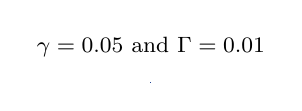
\begin{tikzpicture}[%
font=\footnotesize
]

\begin{axis}[%
width=0.951\figwidth,
height=\figheight,
at={(0\figwidth,0\figheight)},
scale only axis,
xmin=0,
xmax=3,
tick align=outside,
xlabel={Log-Moneyness},
xmajorgrids,
ymin=0,
ymax=5,
ylabel={Remaining Time},
ymajorgrids,
zmin=0,
zmax=6,
zlabel={Optimal Rate},
zmajorgrids,
view={50}{40},
axis background/.style={fill=white},
title={$\gamma = 0.05$ and $\Gamma = 0.01$},
axis x line*=bottom,
axis y line*=left,
axis z line*=left
]

\addplot3[%
surf,
shader=flat corner,draw=black,z buffer=sort,colormap={mymap}{[1pt] rgb(0pt)=(0.2081,0.1663,0.5292); rgb(1pt)=(0.211624,0.189781,0.577676); rgb(2pt)=(0.212252,0.213771,0.626971); rgb(3pt)=(0.2081,0.2386,0.677086); rgb(4pt)=(0.195905,0.264457,0.7279); rgb(5pt)=(0.170729,0.291938,0.779248); rgb(6pt)=(0.125271,0.324243,0.830271); rgb(7pt)=(0.0591333,0.359833,0.868333); rgb(8pt)=(0.0116952,0.38751,0.881957); rgb(9pt)=(0.00595714,0.408614,0.882843); rgb(10pt)=(0.0165143,0.4266,0.878633); rgb(11pt)=(0.0328524,0.443043,0.871957); rgb(12pt)=(0.0498143,0.458571,0.864057); rgb(13pt)=(0.0629333,0.47369,0.855438); rgb(14pt)=(0.0722667,0.488667,0.8467); rgb(15pt)=(0.0779429,0.503986,0.838371); rgb(16pt)=(0.0793476,0.520024,0.831181); rgb(17pt)=(0.0749429,0.537543,0.826271); rgb(18pt)=(0.0640571,0.556986,0.823957); rgb(19pt)=(0.0487714,0.577224,0.822829); rgb(20pt)=(0.0343429,0.596581,0.819852); rgb(21pt)=(0.0265,0.6137,0.8135); rgb(22pt)=(0.0238905,0.628662,0.803762); rgb(23pt)=(0.0230905,0.641786,0.791267); rgb(24pt)=(0.0227714,0.653486,0.776757); rgb(25pt)=(0.0266619,0.664195,0.760719); rgb(26pt)=(0.0383714,0.674271,0.743552); rgb(27pt)=(0.0589714,0.683757,0.725386); rgb(28pt)=(0.0843,0.692833,0.706167); rgb(29pt)=(0.113295,0.7015,0.685857); rgb(30pt)=(0.145271,0.709757,0.664629); rgb(31pt)=(0.180133,0.717657,0.642433); rgb(32pt)=(0.217829,0.725043,0.619262); rgb(33pt)=(0.258643,0.731714,0.595429); rgb(34pt)=(0.302171,0.737605,0.571186); rgb(35pt)=(0.348167,0.742433,0.547267); rgb(36pt)=(0.395257,0.7459,0.524443); rgb(37pt)=(0.44201,0.748081,0.503314); rgb(38pt)=(0.487124,0.749062,0.483976); rgb(39pt)=(0.530029,0.749114,0.466114); rgb(40pt)=(0.570857,0.748519,0.44939); rgb(41pt)=(0.609852,0.747314,0.433686); rgb(42pt)=(0.6473,0.7456,0.4188); rgb(43pt)=(0.683419,0.743476,0.404433); rgb(44pt)=(0.71841,0.741133,0.390476); rgb(45pt)=(0.752486,0.7384,0.376814); rgb(46pt)=(0.785843,0.735567,0.363271); rgb(47pt)=(0.818505,0.732733,0.34979); rgb(48pt)=(0.850657,0.7299,0.336029); rgb(49pt)=(0.882433,0.727433,0.3217); rgb(50pt)=(0.913933,0.725786,0.306276); rgb(51pt)=(0.944957,0.726114,0.288643); rgb(52pt)=(0.973895,0.731395,0.266648); rgb(53pt)=(0.993771,0.745457,0.240348); rgb(54pt)=(0.999043,0.765314,0.216414); rgb(55pt)=(0.995533,0.786057,0.196652); rgb(56pt)=(0.988,0.8066,0.179367); rgb(57pt)=(0.978857,0.827143,0.163314); rgb(58pt)=(0.9697,0.848138,0.147452); rgb(59pt)=(0.962586,0.870514,0.1309); rgb(60pt)=(0.958871,0.8949,0.113243); rgb(61pt)=(0.959824,0.921833,0.0948381); rgb(62pt)=(0.9661,0.951443,0.0755333); rgb(63pt)=(0.9763,0.9831,0.0538)},mesh/rows=25]
table[row sep=crcr, point meta=\thisrow{c}] {%
%
x	y	z	c\\
0	0.01	0.097056830422462	0.097056830422462\\
0	0.111836734693878	0.27074183797763	0.27074183797763\\
0	0.213673469387755	0.3792231343804	0.3792231343804\\
0	0.315510204081633	0.471471127935523	0.471471127935523\\
0	0.41734693877551	0.555742220869033	0.555742220869033\\
0	0.519183673469388	0.635375573634392	0.635375573634392\\
0	0.621020408163265	0.712134730528906	0.712134730528906\\
0	0.722857142857143	0.787098582718	0.787098582718\\
0	0.82469387755102	0.860994165344543	0.860994165344543\\
0	0.926530612244898	0.934346980753216	0.934346980753216\\
0	1.02836734693878	1.00755797333815	1.00755797333815\\
0	1.13020408163265	1.08094666136726	1.08094666136726\\
0	1.23204081632653	1.15477701461901	1.15477701461901\\
0	1.33387755102041	1.22927384003308	1.22927384003308\\
0	1.43571428571429	1.30463362201788	1.30463362201788\\
0	1.53755102040816	1.38103196107275	1.38103196107275\\
0	1.63938775510204	1.45862883955656	1.45862883955656\\
0	1.74122448979592	1.537572451406	1.537572451406\\
0	1.8430612244898	1.61800205472782	1.61800205472782\\
0	1.94489795918367	1.70005014261932	1.70005014261932\\
0	2.04673469387755	1.78384412778838	1.78384412778838\\
0	2.14857142857143	1.86950767374015	1.86950767374015\\
0	2.25040816326531	1.95716176469104	1.95716176469104\\
0	2.35224489795918	2.04692557944842	2.04692557944842\\
0	2.45408163265306	2.13891721627895	2.13891721627895\\
0	2.55591836734694	2.2332543031976	2.2332543031976\\
0	2.65775510204082	2.33005451926945	2.33005451926945\\
0	2.75959183673469	2.42943604621347	2.42943604621347\\
0	2.86142857142857	2.53151796500537	2.53151796500537\\
0	2.96326530612245	2.63642060884048	2.63642060884048\\
0	3.06510204081633	2.74426588130162	2.74426588130162\\
0	3.1669387755102	2.85517754671903	2.85517754671903\\
0	3.26877551020408	2.96928149827848	2.96928149827848\\
0	3.37061224489796	3.08670600833358	3.08670600833358\\
0	3.47244897959184	3.20758196454954	3.20758196454954\\
0	3.57428571428571	3.3320430948365	3.3320430948365\\
0	3.67612244897959	3.46022618351331	3.46022618351331\\
0	3.77795918367347	3.59227128073308	3.59227128073308\\
0	3.87979591836735	3.72832190688527	3.72832190688527\\
0	3.98163265306122	3.86852525340822	3.86852525340822\\
0	4.0834693877551	4.01303238125902	4.01303238125902\\
0	4.18530612244898	4.16199841809058	4.16199841809058\\
0	4.28714285714286	4.31558275507934	4.31558275507934\\
0	4.38897959183674	4.47394924420073	4.47394924420073\\
0	4.49081632653061	4.63726639667736	4.63726639667736\\
0	4.59265306122449	4.80570758325817	4.80570758325817\\
0	4.69448979591837	4.97945123688841	4.97945123688841\\
0	4.79632653061224	5.15868105831644	5.15868105831644\\
0	4.89816326530612	5.34358622513126	5.34358622513126\\
0	5	5.53436160466833	5.53436160466833\\
0.125	0.01	0.0322815326276686	0.0322815326276686\\
0.125	0.111836734693878	0.115834276497288	0.115834276497288\\
0.125	0.213673469387755	0.202324106494922	0.202324106494922\\
0.125	0.315510204081633	0.281136204924216	0.281136204924216\\
0.125	0.41734693877551	0.355066430214883	0.355066430214883\\
0.125	0.519183673469388	0.425841552613698	0.425841552613698\\
0.125	0.621020408163265	0.494542409572329	0.494542409572329\\
0.125	0.722857142857143	0.561896857255647	0.561896857255647\\
0.125	0.82469387755102	0.628427308183484	0.628427308183484\\
0.125	0.926530612244898	0.694528790485154	0.694528790485154\\
0.125	1.02836734693878	0.760513130173516	0.760513130173516\\
0.125	1.13020408163265	0.826635502322237	0.826635502322237\\
0.125	1.23204081632653	0.893111210404943	0.893111210404943\\
0.125	1.33387755102041	0.960126748090449	0.960126748090449\\
0.125	1.43571428571429	1.02784735799475	1.02784735799475\\
0.125	1.53755102040816	1.09642235850659	1.09642235850659\\
0.125	1.63938775510204	1.16598900011685	1.16598900011685\\
0.125	1.74122448979592	1.23667532450037	1.23667532450037\\
0.125	1.8430612244898	1.30860233007806	1.30860233007806\\
0.125	1.94489795918367	1.3818856445559	1.3818856445559\\
0.125	2.04673469387755	1.45663684012663	1.45663684012663\\
0.125	2.14857142857143	1.53296448521712	1.53296448521712\\
0.125	2.25040816326531	1.61097499904137	1.61097499904137\\
0.125	2.35224489795918	1.69077323058123	1.69077323058123\\
0.125	2.45408163265306	1.77246367866618	1.77246367866618\\
0.125	2.55591836734694	1.8561497332004	1.8561497332004\\
0.125	2.65775510204082	1.94193536642148	1.94193536642148\\
0.125	2.75959183673469	2.02992487938569	2.02992487938569\\
0.125	2.86142857142857	2.12022336072855	2.12022336072855\\
0.125	2.96326530612245	2.21293698461136	2.21293698461136\\
0.125	3.06510204081633	2.30817327851868	2.30817327851868\\
0.125	3.1669387755102	2.40604137993553	2.40604137993553\\
0.125	3.26877551020408	2.50665225278894	2.50665225278894\\
0.125	3.37061224489796	2.6101189111239	2.6101189111239\\
0.125	3.47244897959184	2.71655662082192	2.71655662082192\\
0.125	3.57428571428571	2.82608309420111	2.82608309420111\\
0.125	3.67612244897959	2.93881867747881	2.93881867747881\\
0.125	3.77795918367347	3.05488653275677	3.05488653275677\\
0.125	3.87979591836735	3.17441281592944	3.17441281592944\\
0.125	3.98163265306122	3.29752685170698	3.29752685170698\\
0.125	4.0834693877551	3.42436130677597	3.42436130677597\\
0.125	4.18530612244898	3.55505236198326	3.55505236198326\\
0.125	4.28714285714286	3.6897398843168	3.6897398843168\\
0.125	4.38897959183674	3.82856759936567	3.82856759936567\\
0.125	4.49081632653061	3.9716832648663	3.9716832648663\\
0.125	4.59265306122449	4.11923883450024	4.11923883450024\\
0.125	4.69448979591837	4.27139068338381	4.27139068338381\\
0.125	4.79632653061224	4.42829971278208	4.42829971278208\\
0.125	4.89816326530612	4.59013158430582	4.59013158430582\\
0.125	5	4.75705688723611	4.75705688723611\\
0.25	0.01	0.0319391726721112	0.0319391726721112\\
0.25	0.111836734693878	0.0541413919886689	0.0541413919886689\\
0.25	0.213673469387755	0.103883476370502	0.103883476370502\\
0.25	0.315510204081633	0.159837070107732	0.159837070107732\\
0.25	0.41734693877551	0.217143571041487	0.217143571041487\\
0.25	0.519183673469388	0.274637580965345	0.274637580965345\\
0.25	0.621020408163265	0.332053391388742	0.332053391388742\\
0.25	0.722857142857143	0.38939546977001	0.38939546977001\\
0.25	0.82469387755102	0.446756587679783	0.446756587679783\\
0.25	0.926530612244898	0.504256888732398	0.504256888732398\\
0.25	1.02836734693878	0.562021858793119	0.562021858793119\\
0.25	1.13020408163265	0.620174312374616	0.620174312374616\\
0.25	1.23204081632653	0.678831793106726	0.678831793106726\\
0.25	1.33387755102041	0.738106129916588	0.738106129916588\\
0.25	1.43571428571429	0.798103835491491	0.798103835491491\\
0.25	1.53755102040816	0.858926797972818	0.858926797972818\\
0.25	1.63938775510204	0.92067303449917	0.92067303449917\\
0.25	1.74122448979592	0.98343741229989	0.98343741229989\\
0.25	1.8430612244898	1.04731230333859	1.04731230333859\\
0.25	1.94489795918367	1.11238816492989	1.11238816492989\\
0.25	2.04673469387755	1.17875405024694	1.17875405024694\\
0.25	2.14857142857143	1.24649805441527	1.24649805441527\\
0.25	2.25040816326531	1.3157077091147	1.3157077091147\\
0.25	2.35224489795918	1.38647032936026	1.38647032936026\\
0.25	2.45408163265306	1.45887332220988	1.45887332220988\\
0.25	2.55591836734694	1.53300446640932	1.53300446640932\\
0.25	2.65775510204082	1.60895215863908	1.60895215863908\\
0.25	2.75959183673469	1.68680564524399	1.68680564524399\\
0.25	2.86142857142857	1.76665522913725	1.76665522913725\\
0.25	2.96326530612245	1.84859247615091	1.84859247615091\\
0.25	3.06510204081633	1.93271038406223	1.93271038406223\\
0.25	3.1669387755102	2.01910356448772	2.01910356448772\\
0.25	3.26877551020408	2.10786840631114	2.10786840631114\\
0.25	3.37061224489796	2.19910323448482	2.19910323448482\\
0.25	3.47244897959184	2.29290846368998	2.29290846368998\\
0.25	3.57428571428571	2.38938674802027	2.38938674802027\\
0.25	3.67612244897959	2.48864312769041	2.48864312769041\\
0.25	3.77795918367347	2.5907851736373	2.5907851736373\\
0.25	3.87979591836735	2.69592313077024	2.69592313077024\\
0.25	3.98163265306122	2.80417006053477	2.80417006053477\\
0.25	4.0834693877551	2.91564198337801	2.91564198337801\\
0.25	4.18530612244898	3.03045802164012	3.03045802164012\\
0.25	4.28714285714286	3.14874054334358	3.14874054334358\\
0.25	4.38897959183674	3.2706153073077	3.2706153073077\\
0.25	4.49081632653061	3.39621160997967	3.39621160997967\\
0.25	4.59265306122449	3.52566243434241	3.52566243434241\\
0.25	4.69448979591837	3.65910460123462	3.65910460123462\\
0.25	4.79632653061224	3.79667891117931	3.79667891117931\\
0.25	4.89816326530612	3.93853036254489	3.93853036254489\\
0.25	5	4.08480818974095	4.08480818974095\\
0.375	0.01	0.0319391630087627	0.0319391630087627\\
0.375	0.111836734693878	0.0380871579823106	0.0380871579823106\\
0.375	0.213673469387755	0.0596602613259123	0.0596602613259123\\
0.375	0.315510204081633	0.0926393278360963	0.0926393278360963\\
0.375	0.41734693877551	0.131600828200854	0.131600828200854\\
0.375	0.519183673469388	0.173930528872596	0.173930528872596\\
0.375	0.621020408163265	0.218363120025686	0.218363120025686\\
0.375	0.722857142857143	0.264253798215795	0.264253798215795\\
0.375	0.82469387755102	0.311263646510582	0.311263646510582\\
0.375	0.926530612244898	0.359215386503389	0.359215386503389\\
0.375	1.02836734693878	0.408022306085388	0.408022306085388\\
0.375	1.13020408163265	0.457650954907669	0.457650954907669\\
0.375	1.23204081632653	0.508100504276959	0.508100504276959\\
0.375	1.33387755102041	0.559390821032293	0.559390821032293\\
0.375	1.43571428571429	0.611555327417646	0.611555327417646\\
0.375	1.53755102040816	0.664636601489144	0.664636601489144\\
0.375	1.63938775510204	0.718683603632646	0.718683603632646\\
0.375	1.74122448979592	0.773749897880173	0.773749897880173\\
0.375	1.8430612244898	0.829892498099618	0.829892498099618\\
0.375	1.94489795918367	0.887171115816762	0.887171115816762\\
0.375	2.04673469387755	0.945647671430705	0.945647671430705\\
0.375	2.14857142857143	1.00538598125881	1.00538598125881\\
0.375	2.25040816326531	1.06645156382815	1.06645156382815\\
0.375	2.35224489795918	1.12891152820155	1.12891152820155\\
0.375	2.45408163265306	1.19283451948392	1.19283451948392\\
0.375	2.55591836734694	1.25829070468277	1.25829070468277\\
0.375	2.65775510204082	1.32535178739717	1.32535178739717\\
0.375	2.75959183673469	1.39409104336117	1.39409104336117\\
0.375	2.86142857142857	1.46458337127969	1.46458337127969\\
0.375	2.96326530612245	1.53690535505278	1.53690535505278\\
0.375	3.06510204081633	1.61113533463551	1.61113533463551\\
0.375	3.1669387755102	1.68735348358971	1.68735348358971\\
0.375	3.26877551020408	1.76564189195576	1.76564189195576\\
0.375	3.37061224489796	1.84608465348157	1.84608465348157\\
0.375	3.47244897959184	1.92876795653967	1.92876795653967\\
0.375	3.57428571428571	2.01378017827648	2.01378017827648\\
0.375	3.67612244897959	2.10121198169285	2.10121198169285\\
0.375	3.77795918367347	2.19115641546885	2.19115641546885\\
0.375	3.87979591836735	2.28370901642974	2.28370901642974\\
0.375	3.98163265306122	2.3789679146123	2.3789679146123\\
0.375	4.0834693877551	2.4770339409373	2.4770339409373\\
0.375	4.18530612244898	2.57801073752867	2.57801073752867\\
0.375	4.28714285714286	2.68200487074647	2.68200487074647\\
0.375	4.38897959183674	2.78912594743093	2.78912594743093\\
0.375	4.49081632653061	2.89948673235451	2.89948673235451\\
0.375	4.59265306122449	3.01320327141965	3.01320327141965\\
0.375	4.69448979591837	3.1303950158775	3.1303950158775\\
0.375	4.79632653061224	3.25118495062035	3.25118495062035\\
0.375	4.89816326530612	3.37569972577811	3.37569972577811\\
0.375	5	3.50406979187719	3.50406979187719\\
0.5	0.01	0.0319391630087619	0.0319391630087619\\
0.5	0.111836734693878	0.0354602352957237	0.0354602352957237\\
0.5	0.213673469387755	0.0439354915373327	0.0439354915373327\\
0.5	0.315510204081633	0.0606997059408904	0.0606997059408904\\
0.5	0.41734693877551	0.0841859330908061	0.0841859330908061\\
0.5	0.519183673469388	0.112499220592102	0.112499220592102\\
0.5	0.621020408163265	0.144308152876515	0.144308152876515\\
0.5	0.722857142857143	0.178745025197592	0.178745025197592\\
0.5	0.82469387755102	0.215246762499028	0.215246762499028\\
0.5	0.926530612244898	0.253444770815062	0.253444770815062\\
0.5	1.02836734693878	0.29309620799383	0.29309620799383\\
0.5	1.13020408163265	0.334041470083607	0.334041470083607\\
0.5	1.23204081632653	0.376177474848909	0.376177474848909\\
0.5	1.33387755102041	0.419440491678632	0.419440491678632\\
0.5	1.43571428571429	0.463794846878427	0.463794846878427\\
0.5	1.53755102040816	0.509225328076412	0.509225328076412\\
0.5	1.63938775510204	0.555731972341564	0.555731972341564\\
0.5	1.74122448979592	0.603326425013763	0.603326425013763\\
0.5	1.8430612244898	0.652029355331037	0.652029355331037\\
0.5	1.94489795918367	0.701868596917169	0.701868596917169\\
0.5	2.04673469387755	0.752877794353119	0.752877794353119\\
0.5	2.14857142857143	0.805095408908853	0.805095408908853\\
0.5	2.25040816326531	0.858563983043728	0.858563983043728\\
0.5	2.35224489795918	0.913329593976202	0.913329593976202\\
0.5	2.45408163265306	0.969441447217738	0.969441447217738\\
0.5	2.55591836734694	1.02695157500506	1.02695157500506\\
0.5	2.65775510204082	1.08591461427752	1.08591461427752\\
0.5	2.75959183673469	1.14638764565843	1.14638764565843\\
0.5	2.86142857142857	1.20843007973803	1.20843007973803\\
0.5	2.96326530612245	1.27210358043377	1.27210358043377\\
0.5	3.06510204081633	1.33747201773182	1.33747201773182\\
0.5	3.1669387755102	1.40460144396995	1.40460144396995\\
0.5	3.26877551020408	1.47356008919862	1.47356008919862\\
0.5	3.37061224489796	1.54441837218748	1.54441837218748\\
0.5	3.47244897959184	1.61724892442196	1.61724892442196\\
0.5	3.57428571428571	1.69212662502649	1.69212662502649\\
0.5	3.67612244897959	1.76912864500499	1.76912864500499\\
0.5	3.77795918367347	1.84833449953956	1.84833449953956\\
0.5	3.87979591836735	1.92982610736172	1.92982610736172\\
0.5	3.98163265306122	2.01368785642403	2.01368785642403\\
0.5	4.0834693877551	2.10000667526891	2.10000667526891\\
0.5	4.18530612244898	2.18887210962523	2.18887210962523\\
0.5	4.28714285714286	2.28037640387062	2.28037640387062\\
0.5	4.38897959183674	2.37461458708328	2.37461458708328\\
0.5	4.49081632653061	2.47168456347722	2.47168456347722\\
0.5	4.59265306122449	2.5716872070716	2.5716872070716\\
0.5	4.69448979591837	2.67472646049166	2.67472646049166\\
0.5	4.79632653061224	2.78090943783738	2.78090943783738\\
0.5	4.89816326530612	2.89034653158852	2.89034653158852\\
0.5	5	3.0031515235416	3.0031515235416\\
0.625	0.01	0.0319391630087619	0.0319391630087619\\
0.625	0.111836734693878	0.0351964642072958	0.0351964642072958\\
0.625	0.213673469387755	0.0395701480823777	0.0395701480823777\\
0.625	0.315510204081633	0.0477996122095189	0.0477996122095189\\
0.625	0.41734693877551	0.0608730943715396	0.0608730943715396\\
0.625	0.519183673469388	0.0783869939702372	0.0783869939702372\\
0.625	0.621020408163265	0.0996320413157746	0.0996320413157746\\
0.625	0.722857142857143	0.12395952990427	0.12395952990427\\
0.625	0.82469387755102	0.15085345220286	0.15085345220286\\
0.625	0.926530612244898	0.179921663399059	0.179921663399059\\
0.625	1.02836734693878	0.210871119476097	0.210871119476097\\
0.625	1.13020408163265	0.243484481363642	0.243484481363642\\
0.625	1.23204081632653	0.277601563716369	0.277601563716369\\
0.625	1.33387755102041	0.31310541547646	0.31310541547646\\
0.625	1.43571428571429	0.349912056954104	0.349912056954104\\
0.625	1.53755102040816	0.387962930756993	0.387962930756993\\
0.625	1.63938775510204	0.427219324911	0.427219324911\\
0.625	1.74122448979592	0.467658222851552	0.467658222851552\\
0.625	1.8430612244898	0.509269189103053	0.509269189103053\\
0.625	1.94489795918367	0.552052011962465	0.552052011962465\\
0.625	2.04673469387755	0.596014904355217	0.596014904355217\\
0.625	2.14857142857143	0.641173120198751	0.641173120198751\\
0.625	2.25040816326531	0.687547883113272	0.687547883113272\\
0.625	2.35224489795918	0.735165552230053	0.735165552230053\\
0.625	2.45408163265306	0.784056969704857	0.784056969704857\\
0.625	2.55591836734694	0.834256948787598	0.834256948787598\\
0.625	2.65775510204082	0.885803871605989	0.885803871605989\\
0.625	2.75959183673469	0.938739373345832	0.938739373345832\\
0.625	2.86142857142857	0.993108095053446	0.993108095053446\\
0.625	2.96326530612245	1.04895749140445	1.04895749140445\\
0.625	3.06510204081633	1.10633768286949	1.10633768286949\\
0.625	3.1669387755102	1.16530134403911	1.16530134403911\\
0.625	3.26877551020408	1.22590362164579	1.22590362164579\\
0.625	3.37061224489796	1.28820207718281	1.28820207718281\\
0.625	3.47244897959184	1.35225665007282	1.35225665007282\\
0.625	3.57428571428571	1.41812963815759	1.41812963815759\\
0.625	3.67612244897959	1.48588569292225	1.48588569292225\\
0.625	3.77795918367347	1.55559182737329	1.55559182737329\\
0.625	3.87979591836735	1.6273174348904	1.6273174348904\\
0.625	3.98163265306122	1.701134317693	1.701134317693\\
0.625	4.0834693877551	1.77711672381877	1.77711672381877\\
0.625	4.18530612244898	1.85534139171932	1.85534139171932\\
0.625	4.28714285714286	1.9358876017463	1.9358876017463\\
0.625	4.38897959183674	2.01883723393887	2.01883723393887\\
0.625	4.49081632653061	2.10427483163586	2.10427483163586\\
0.625	4.59265306122449	2.19228767052954	2.19228767052954\\
0.625	4.69448979591837	2.28296583285451	2.28296583285451\\
0.625	4.79632653061224	2.37640228647	2.37640228647\\
0.625	4.89816326530612	2.47269296864776	2.47269296864776\\
0.625	5	2.57193687442325	2.57193687442325\\
0.75	0.01	0.0319391630087619	0.0319391630087619\\
0.75	0.111836734693878	0.0351804715524161	0.0351804715524161\\
0.75	0.213673469387755	0.0386330520482968	0.0386330520482968\\
0.75	0.315510204081633	0.0434035662239544	0.0434035662239544\\
0.75	0.41734693877551	0.0507628976357168	0.0507628976357168\\
0.75	0.519183673469388	0.0612254626069931	0.0612254626069931\\
0.75	0.621020408163265	0.0747720380184666	0.0747720380184666\\
0.75	0.722857142857143	0.0911661632720615	0.0911661632720615\\
0.75	0.82469387755102	0.110118075668323	0.110118075668323\\
0.75	0.926530612244898	0.131351747786388	0.131351747786388\\
0.75	1.02836734693878	0.154627359673547	0.154627359673547\\
0.75	1.13020408163265	0.179745368355871	0.179745368355871\\
0.75	1.23204081632653	0.206543676642299	0.206543676642299\\
0.75	1.33387755102041	0.234892712415608	0.234892712415608\\
0.75	1.43571428571429	0.264690334794864	0.264690334794864\\
0.75	1.53755102040816	0.295857256886145	0.295857256886145\\
0.75	1.63938775510204	0.32833316729109	0.32833316729109\\
0.75	1.74122448979592	0.362073533416459	0.362073533416459\\
0.75	1.8430612244898	0.397047001537487	0.397047001537487\\
0.75	1.94489795918367	0.433233294603844	0.433233294603844\\
0.75	2.04673469387755	0.470621515616352	0.470621515616352\\
0.75	2.14857142857143	0.509208777803839	0.509208777803839\\
0.75	2.25040816326531	0.548999096945766	0.548999096945766\\
0.75	2.35224489795918	0.590002493845423	0.590002493845423\\
0.75	2.45408163265306	0.632234265561936	0.632234265561936\\
0.75	2.55591836734694	0.675714392595281	0.675714392595281\\
0.75	2.65775510204082	0.720467056049038	0.720467056049038\\
0.75	2.75959183673469	0.766520244181336	0.766520244181336\\
0.75	2.86142857142857	0.813905431984181	0.813905431984181\\
0.75	2.96326530612245	0.862657320750714	0.862657320750714\\
0.75	3.06510204081633	0.912813627197567	0.912813627197567\\
0.75	3.1669387755102	0.964414913763066	0.964414913763066\\
0.75	3.26877551020408	1.0175044533243	1.0175044533243\\
0.75	3.37061224489796	1.0721281228625	1.0721281228625\\
0.75	3.47244897959184	1.12833432163045	1.12833432163045\\
0.75	3.57428571428571	1.18617391019435	1.18617391019435\\
0.75	3.67612244897959	1.24570016738052	1.24570016738052\\
0.75	3.77795918367347	1.30696876268753	1.30696876268753\\
0.75	3.87979591836735	1.37003774215414	1.37003774215414\\
0.75	3.98163265306122	1.43496752602356	1.43496752602356\\
0.75	4.0834693877551	1.50182091682977	1.50182091682977\\
0.75	4.18530612244898	1.57066311676712	1.57066311676712\\
0.75	4.28714285714286	1.64156175339737	1.64156175339737\\
0.75	4.38897959183674	1.71458691290893	1.71458691290893\\
0.75	4.49081632653061	1.78981118027624	1.78981118027624\\
0.75	4.59265306122449	1.8673096857788	1.8673096857788\\
0.75	4.69448979591837	1.94716015743246	1.94716015743246\\
0.75	4.79632653061224	2.02944297896477	2.02944297896477\\
0.75	4.89816326530612	2.11424125303246	2.11424125303246\\
0.75	5	2.20164086943613	2.20164086943613\\
0.875	0.01	0.0319391630087619	0.0319391630087619\\
0.875	0.111836734693878	0.0351798926066943	0.0351798926066943\\
0.875	0.213673469387755	0.0384785585896546	0.0384785585896546\\
0.875	0.315510204081633	0.0421462168256953	0.0421462168256953\\
0.875	0.41734693877551	0.0469123030473164	0.0469123030473164\\
0.875	0.519183673469388	0.0534322548274285	0.0534322548274285\\
0.875	0.621020408163265	0.0620542060001257	0.0620542060001257\\
0.875	0.722857142857143	0.0728810372203625	0.0728810372203625\\
0.875	0.82469387755102	0.0858755060045674	0.0858755060045674\\
0.875	0.926530612244898	0.100934301282865	0.100934301282865\\
0.875	1.02836734693878	0.117930542375621	0.117930542375621\\
0.875	1.13020408163265	0.136735923582582	0.136735923582582\\
0.875	1.23204081632653	0.157231315778604	0.157231315778604\\
0.875	1.33387755102041	0.179311183380251	0.179311183380251\\
0.875	1.43571428571429	0.202884816665406	0.202884816665406\\
0.875	1.53755102040816	0.22787600206369	0.22787600206369\\
0.875	1.63938775510204	0.25422199076111	0.25422199076111\\
0.875	1.74122448979592	0.281872212766045	0.281872212766045\\
0.875	1.8430612244898	0.310786961674127	0.310786961674127\\
0.875	1.94489795918367	0.340936157058954	0.340936157058954\\
0.875	2.04673469387755	0.372298229054472	0.372298229054472\\
0.875	2.14857142857143	0.40485913753377	0.40485913753377\\
0.875	2.25040816326531	0.438611522394574	0.438611522394574\\
0.875	2.35224489795918	0.473553974267883	0.473553974267883\\
0.875	2.45408163265306	0.509690412352896	0.509690412352896\\
0.875	2.55591836734694	0.547029555804082	0.547029555804082\\
0.875	2.65775510204082	0.585584475938053	0.585584475938053\\
0.875	2.75959183673469	0.62537221783623	0.62537221783623\\
0.875	2.86142857142857	0.666413481353236	0.666413481353236\\
0.875	2.96326530612245	0.708732352929958	0.708732352929958\\
0.875	3.06510204081633	0.752356080877085	0.752356080877085\\
0.875	3.1669387755102	0.797314887911981	0.797314887911981\\
0.875	3.26877551020408	0.843641815696809	0.843641815696809\\
0.875	3.37061224489796	0.891372596949228	0.891372596949228\\
0.875	3.47244897959184	0.940545551394068	0.940545551394068\\
0.875	3.57428571428571	0.991201502411674	0.991201502411674\\
0.875	3.67612244897959	1.04338371173224	1.04338371173224\\
0.875	3.77795918367347	1.09713782993975	1.09713782993975\\
0.875	3.87979591836735	1.15251186089709	1.15251186089709\\
0.875	3.98163265306122	1.20955613849588	1.20955613849588\\
0.875	4.0834693877551	1.2683233143805	1.2683233143805\\
0.875	4.18530612244898	1.3288683555028	1.3288683555028\\
0.875	4.28714285714286	1.39124855053879	1.39124855053879\\
0.875	4.38897959183674	1.45552352434647	1.45552352434647\\
0.875	4.49081632653061	1.52175525976975	1.52175525976975\\
0.875	4.59265306122449	1.5900081261999	1.5900081261999\\
0.875	4.69448979591837	1.66034891439737	1.66034891439737\\
0.875	4.79632653061224	1.73284687715455	1.73284687715455\\
0.875	4.89816326530612	1.80757377544733	1.80757377544733\\
0.875	5	1.88460392978069	1.88460392978069\\
1	0.01	0.0319391630087619	0.0319391630087619\\
1	0.111836734693878	0.0351798801956734	0.0351798801956734\\
1	0.213673469387755	0.0384590948586436	0.0384590948586436\\
1	0.315510204081633	0.0418455653340004	0.0418455653340004\\
1	0.41734693877551	0.0456286273686764	0.0456286273686764\\
1	0.519183673469388	0.0502471153099599	0.0502471153099599\\
1	0.621020408163265	0.0560882186125518	0.0560882186125518\\
1	0.722857142857143	0.063406137058125	0.063406137058125\\
1	0.82469387755102	0.0723325088949056	0.0723325088949056\\
1	0.926530612244898	0.0829121045337091	0.0829121045337091\\
1	1.02836734693878	0.0951356830461746	0.0951356830461746\\
1	1.13020408163265	0.108963755848085	0.108963755848085\\
1	1.23204081632653	0.124342150898328	0.124342150898328\\
1	1.33387755102041	0.141211656165434	0.141211656165434\\
1	1.43571428571429	0.15951374096221	0.15951374096221\\
1	1.53755102040816	0.179193786947916	0.179193786947916\\
1	1.63938775510204	0.200202778069601	0.200202778069601\\
1	1.74122448979592	0.222498056641012	0.222498056641012\\
1	1.8430612244898	0.246043526798415	0.246043526798415\\
1	1.94489795918367	0.270809541995875	0.270809541995875\\
1	2.04673469387755	0.296772622083124	0.296772622083124\\
1	2.14857142857143	0.323915088499349	0.323915088499349\\
1	2.25040816326531	0.352224670589218	0.352224670589218\\
1	2.35224489795918	0.381694113980157	0.381694113980157\\
1	2.45408163265306	0.412320808313477	0.412320808313477\\
1	2.55591836734694	0.44410644324477	0.44410644324477\\
1	2.65775510204082	0.477056696549689	0.477056696549689\\
1	2.75959183673469	0.511180955154702	0.511180955154702\\
1	2.86142857142857	0.54649206818272	0.54649206818272\\
1	2.96326530612245	0.583006130172145	0.583006130172145\\
1	3.06510204081633	0.620742292186674	0.620742292186674\\
1	3.1669387755102	0.659722598387919	0.659722598387919\\
1	3.26877551020408	0.699971845671069	0.699971845671069\\
1	3.37061224489796	0.74151746408886	0.74151746408886\\
1	3.47244897959184	0.784389415963355	0.784389415963355\\
1	3.57428571428571	0.828620111779307	0.828620111779307\\
1	3.67612244897959	0.8742443411498	0.8742443411498\\
1	3.77795918367347	0.921299217334452	0.921299217334452\\
1	3.87979591836735	0.969824133967325	0.969824133967325\\
1	3.98163265306122	1.01986073281345	1.01986073281345\\
1	4.0834693877551	1.07145288151882	1.07145288151882\\
1	4.18530612244898	1.12464666044919	1.12464666044919\\
1	4.28714285714286	1.17949035782883	1.17949035782883\\
1	4.38897959183674	1.23603447249297	1.23603447249297\\
1	4.49081632653061	1.29433172365809	1.29433172365809\\
1	4.59265306122449	1.35443706719384	1.35443706719384\\
1	4.69448979591837	1.41640771795041	1.41640771795041\\
1	4.79632653061224	1.48030317775705	1.48030317775705\\
1	4.89816326530612	1.54618526876153	1.54618526876153\\
1	5	1.6141181718285	1.6141181718285\\
1.125	0.01	0.0319391630087619	0.0319391630087619\\
1.125	0.111836734693878	0.0351798800390967	0.0351798800390967\\
1.125	0.213673469387755	0.0384572280310823	0.0384572280310823\\
1.125	0.315510204081633	0.0417856439540207	0.0417856439540207\\
1.125	0.41734693877551	0.0452550147595181	0.0452550147595181\\
1.125	0.519183673469388	0.0490781618037211	0.0490781618037211\\
1.125	0.621020408163265	0.0535272357779093	0.0535272357779093\\
1.125	0.722857142857143	0.0588522111537542	0.0588522111537542\\
1.125	0.82469387755102	0.0652431426637235	0.0652431426637235\\
1.125	0.926530612244898	0.0728266362207302	0.0728266362207302\\
1.125	1.02836734693878	0.0816767065971522	0.0816767065971522\\
1.125	1.13020408163265	0.0918286011377671	0.0918286011377671\\
1.125	1.23204081632653	0.103291052304197	0.103291052304197\\
1.125	1.33387755102041	0.116055795360844	0.116055795360844\\
1.125	1.43571428571429	0.130104491564996	0.130104491564996\\
1.125	1.53755102040816	0.145413570924075	0.145413570924075\\
1.125	1.63938775510204	0.161957526466543	0.161957526466543\\
1.125	1.74122448979592	0.179711100410817	0.179711100410817\\
1.125	1.8430612244898	0.198650695686919	0.198650695686919\\
1.125	1.94489795918367	0.21875525441849	0.21875525441849\\
1.125	2.04673469387755	0.240006774279513	0.240006774279513\\
1.125	2.14857142857143	0.262390581964711	0.262390581964711\\
1.125	2.25040816326531	0.285895446245401	0.285895446245401\\
1.125	2.35224489795918	0.310513587305761	0.310513587305761\\
1.125	2.45408163265306	0.336240621129558	0.336240621129558\\
1.125	2.55591836734694	0.363075465298691	0.363075465298691\\
1.125	2.65775510204082	0.391020223996996	0.391020223996996\\
1.125	2.75959183673469	0.420080064107427	0.420080064107427\\
1.125	2.86142857142857	0.450263090227596	0.450263090227596\\
1.125	2.96326530612245	0.481580223639843	0.481580223639843\\
1.125	3.06510204081633	0.51404508836475	0.51404508836475\\
1.125	3.1669387755102	0.547673906130091	0.547673906130091\\
1.125	3.26877551020408	0.582485401212757	0.582485401212757\\
1.125	3.37061224489796	0.61850071552923	0.61850071552923\\
1.125	3.47244897959184	0.655743333970346	0.655743333970346\\
1.125	3.57428571428571	0.694239019735547	0.694239019735547\\
1.125	3.67612244897959	0.734015759276981	0.734015759276981\\
1.125	3.77795918367347	0.775103716384073	0.775103716384073\\
1.125	3.87979591836735	0.817535194903395	0.817535194903395\\
1.125	3.98163265306122	0.861344609582031	0.861344609582031\\
1.125	4.0834693877551	0.906568464534901	0.906568464534901\\
1.125	4.18530612244898	0.953245338860513	0.953245338860513\\
1.125	4.28714285714286	1.00141587896059	1.00141587896059\\
1.125	4.38897959183674	1.05112279715355	1.05112279715355\\
1.125	4.49081632653061	1.1024108762076	1.1024108762076\\
1.125	4.59265306122449	1.15532697945518	1.15532697945518\\
1.125	4.69448979591837	1.20992006618492	1.20992006618492\\
1.125	4.79632653061224	1.2662412120405	1.2662412120405\\
1.125	4.89816326530612	1.32434363418697	1.32434363418697\\
1.125	5	1.38428272103404	1.38428272103404\\
1.25	0.01	0.0319391630087619	0.0319391630087619\\
1.25	0.111836734693878	0.0351798800379398	0.0351798800379398\\
1.25	0.213673469387755	0.0384570921086942	0.0384570921086942\\
1.25	0.315510204081633	0.0417757127315871	0.0417757127315871\\
1.25	0.41734693877551	0.0451602718234656	0.0451602718234656\\
1.25	0.519183673469388	0.0486936312262368	0.0486936312262368\\
1.25	0.621020408163265	0.0525229432947096	0.0525229432947096\\
1.25	0.722857142857143	0.0568251935063542	0.0568251935063542\\
1.25	0.82469387755102	0.0617707927955668	0.0617707927955668\\
1.25	0.926530612244898	0.0675032438584044	0.0675032438584044\\
1.25	1.02836734693878	0.074133041689348	0.074133041689348\\
1.25	1.13020408163265	0.0817395428502374	0.0817395428502374\\
1.25	1.23204081632653	0.0903760820209085	0.0903760820209085\\
1.25	1.33387755102041	0.100075747138493	0.100075747138493\\
1.25	1.43571428571429	0.110856654060268	0.110856654060268\\
1.25	1.53755102040816	0.122726329241687	0.122726329241687\\
1.25	1.63938775510204	0.13568516730215	0.13568516730215\\
1.25	1.74122448979592	0.149729072814922	0.149729072814922\\
1.25	1.8430612244898	0.164851435061634	0.164851435061634\\
1.25	1.94489795918367	0.18104457958931	0.18104457958931\\
1.25	2.04673469387755	0.198300819604415	0.198300819604415\\
1.25	2.14857142857143	0.216613206305415	0.216613206305415\\
1.25	2.25040816326531	0.235976055344224	0.235976055344224\\
1.25	2.35224489795918	0.256385308345059	0.256385308345059\\
1.25	2.45408163265306	0.277838773906771	0.277838773906771\\
1.25	2.55591836734694	0.300336281310172	0.300336281310172\\
1.25	2.65775510204082	0.323879771636947	0.323879771636947\\
1.25	2.75959183673469	0.348473344600822	0.348473344600822\\
1.25	2.86142857142857	0.374123274602417	0.374123274602417\\
1.25	2.96326530612245	0.400838005952312	0.400838005952312\\
1.25	3.06510204081633	0.428628134556628	0.428628134556628\\
1.25	3.1669387755102	0.457506381393241	0.457506381393241\\
1.25	3.26877551020408	0.487487561649655	0.487487561649655\\
1.25	3.37061224489796	0.518588552314832	0.518588552314832\\
1.25	3.47244897959184	0.550828260219709	0.550828260219709\\
1.25	3.57428571428571	0.584227591932417	0.584227591932417\\
1.25	3.67612244897959	0.61880942648074	0.61880942648074\\
1.25	3.77795918367347	0.654598591556423	0.654598591556423\\
1.25	3.87979591836735	0.691621843623764	0.691621843623764\\
1.25	3.98163265306122	0.729907852186769	0.729907852186769\\
1.25	4.0834693877551	0.769487188348433	0.769487188348433\\
1.25	4.18530612244898	0.810392317710338	0.810392317710338\\
1.25	4.28714285714286	0.852657597601592	0.852657597601592\\
1.25	4.38897959183674	0.896319278586329	0.896319278586329\\
1.25	4.49081632653061	0.941415510173534	0.941415510173534\\
1.25	4.59265306122449	0.98798635063797	0.98798635063797\\
1.25	4.69448979591837	1.03607378085366	1.03607378085366\\
1.25	4.79632653061224	1.08572172203956	1.08572172203956\\
1.25	4.89816326530612	1.13697605731933	1.13697605731933\\
1.25	5	1.1898846570017	1.1898846570017\\
1.375	0.01	0.0319391630087619	0.0319391630087619\\
1.375	0.111836734693878	0.0351798800379348	0.0351798800379348\\
1.375	0.213673469387755	0.0384570846132478	0.0384570846132478\\
1.375	0.315510204081633	0.0417743464770461	0.0417743464770461\\
1.375	0.41734693877551	0.0451393724993173	0.0451393724993173\\
1.375	0.519183673469388	0.0485804189107275	0.0485804189107275\\
1.375	0.621020408163265	0.0521636455151643	0.0521636455151643\\
1.375	0.722857142857143	0.055990670921367	0.055990670921367\\
1.375	0.82469387755102	0.0601813615669343	0.0601813615669343\\
1.375	0.926530612244898	0.0648560341217889	0.0648560341217889\\
1.375	1.02836734693878	0.0701237112511071	0.0701237112511071\\
1.375	1.13020408163265	0.0760766465172827	0.0760766465172827\\
1.375	1.23204081632653	0.0827891827581806	0.0827891827581806\\
1.375	1.33387755102041	0.090319019429548	0.090319019429548\\
1.375	1.43571428571429	0.098709551343763	0.098709551343763\\
1.375	1.53755102040816	0.1079924928858	0.1079924928858\\
1.375	1.63938775510204	0.118190382144712	0.118190382144712\\
1.375	1.74122448979592	0.12931878783853	0.12931878783853\\
1.375	1.8430612244898	0.141388166958487	0.141388166958487\\
1.375	1.94489795918367	0.154405383491553	0.154405383491553\\
1.375	2.04673469387755	0.168374925745865	0.168374925745865\\
1.375	2.14857142857143	0.183299868294564	0.183299868294564\\
1.375	2.25040816326531	0.199182623855645	0.199182623855645\\
1.375	2.35224489795918	0.216025525719148	0.216025525719148\\
1.375	2.45408163265306	0.233831275317938	0.233831275317938\\
1.375	2.55591836734694	0.252603283535359	0.252603283535359\\
1.375	2.65775510204082	0.272345928931467	0.272345928931467\\
1.375	2.75959183673469	0.293064751445141	0.293064751445141\\
1.375	2.86142857142857	0.314766596300344	0.314766596300344\\
1.375	2.96326530612245	0.337459719736699	0.337459719736699\\
1.375	3.06510204081633	0.361153865694037	0.361153865694037\\
1.375	3.1669387755102	0.385860320602083	0.385860320602083\\
1.375	3.26877551020408	0.411591951863752	0.411591951863752\\
1.375	3.37061224489796	0.438363234391059	0.438363234391059\\
1.375	3.47244897959184	0.466190268587863	0.466190268587863\\
1.375	3.57428571428571	0.495090792417918	0.495090792417918\\
1.375	3.67612244897959	0.525084189605445	0.525084189605445\\
1.375	3.77795918367347	0.556191495553293	0.556191495553293\\
1.375	3.87979591836735	0.588435402202812	0.588435402202812\\
1.375	3.98163265306122	0.621840262777863	0.621840262777863\\
1.375	4.0834693877551	0.656432097135882	0.656432097135882\\
1.375	4.18530612244898	0.692238598277916	0.692238598277916\\
1.375	4.28714285714286	0.729289140436765	0.729289140436765\\
1.375	4.38897959183674	0.767614789059383	0.767614789059383\\
1.375	4.49081632653061	0.80724831292017	0.80724831292017\\
1.375	4.59265306122449	0.848224198540612	0.848224198540612\\
1.375	4.69448979591837	0.89057866704398	0.89057866704398\\
1.375	4.79632653061224	0.934349693538375	0.934349693538375\\
1.375	4.89816326530612	0.979577029094815	0.979577029094815\\
1.375	5	1.02630222536749	1.02630222536749\\
1.5	0.01	0.0319391630087619	0.0319391630087619\\
1.5	0.111836734693878	0.0351798800379348	0.0351798800379348\\
1.5	0.213673469387755	0.038457084300765	0.038457084300765\\
1.5	0.315510204081633	0.0417741906896984	0.0417741906896984\\
1.5	0.41734693877551	0.04513536738254	0.04513536738254\\
1.5	0.519183673469388	0.0485506220818049	0.0485506220818049\\
1.5	0.621020408163265	0.0520465045751911	0.0520465045751911\\
1.5	0.722857142857143	0.0556732219395899	0.0556732219395899\\
1.5	0.82469387755102	0.0595021102030488	0.0595021102030488\\
1.5	0.926530612244898	0.0636170031964177	0.0636170031964177\\
1.5	1.02836734693878	0.0681049639087754	0.0681049639087754\\
1.5	1.13020408163265	0.0730492718677155	0.0730492718677155\\
1.5	1.23204081632653	0.0785252303351714	0.0785252303351714\\
1.5	1.33387755102041	0.084598290304585	0.084598290304585\\
1.5	1.43571428571429	0.0913237466267467	0.0913237466267467\\
1.5	1.53755102040816	0.0987473624490123	0.0987473624490123\\
1.5	1.63938775510204	0.106906461949457	0.106906461949457\\
1.5	1.74122448979592	0.115831196960731	0.115831196960731\\
1.5	1.8430612244898	0.125545815013101	0.125545815013101\\
1.5	1.94489795918367	0.136069837377234	0.136069837377234\\
1.5	2.04673469387755	0.147419105996293	0.147419105996293\\
1.5	2.14857142857143	0.15960668761834	0.15960668761834\\
1.5	2.25040816326531	0.172643639509526	0.172643639509526\\
1.5	2.35224489795918	0.186539649041361	0.186539649041361\\
1.5	2.45408163265306	0.201303562580147	0.201303562580147\\
1.5	2.55591836734694	0.216943819576748	0.216943819576748\\
1.5	2.65775510204082	0.233468806840827	0.233468806840827\\
1.5	2.75959183673469	0.250887146438442	0.250887146438442\\
1.5	2.86142857142857	0.269207928902018	0.269207928902018\\
1.5	2.96326530612245	0.288440901716858	0.288440901716858\\
1.5	3.06510204081633	0.308596621461917	0.308596621461917\\
1.5	3.1669387755102	0.329686576581051	0.329686576581051\\
1.5	3.26877551020408	0.351723286554227	0.351723286554227\\
1.5	3.37061224489796	0.374720382216634	0.374720382216634\\
1.5	3.47244897959184	0.398692671119138	0.398692671119138\\
1.5	3.57428571428571	0.423656191114585	0.423656191114585\\
1.5	3.67612244897959	0.449628254769828	0.449628254769828\\
1.5	3.77795918367347	0.476627486723251	0.476627486723251\\
1.5	3.87979591836735	0.504673855714571	0.504673855714571\\
1.5	3.98163265306122	0.533788702692694	0.533788702692694\\
1.5	4.0834693877551	0.563994766145682	0.563994766145682\\
1.5	4.18530612244898	0.595316205583734	0.595316205583734\\
1.5	4.28714285714286	0.62777862393273	0.62777862393273\\
1.5	4.38897959183674	0.661409089454948	0.661409089454948\\
1.5	4.49081632653061	0.696236157699162	0.696236157699162\\
1.5	4.59265306122449	0.732289893889537	0.732289893889537\\
1.5	4.69448979591837	0.769601896087504	0.769601896087504\\
1.5	4.79632653061224	0.80820531940002	0.80820531940002\\
1.5	4.89816326530612	0.848134901458476	0.848134901458476\\
1.5	5	0.889426989352979	0.889426989352979\\
1.625	0.01	0.0319391630087619	0.0319391630087619\\
1.625	0.111836734693878	0.0351798800379348	0.0351798800379348\\
1.625	0.213673469387755	0.0384570842909312	0.0384570842909312\\
1.625	0.315510204081633	0.0417741759839725	0.0417741759839725\\
1.625	0.41734693877551	0.0451347012858541	0.0451347012858541\\
1.625	0.519183673469388	0.0485436182187085	0.0485436182187085\\
1.625	0.621020408163265	0.0520117328420352	0.0520117328420352\\
1.625	0.722857142857143	0.0555617440044286	0.0555617440044286\\
1.625	0.82469387755102	0.0592313218164921	0.0592313218164921\\
1.625	0.926530612244898	0.063071592600241	0.063071592600241\\
1.625	1.02836734693878	0.0671427366167201	0.0671427366167201\\
1.625	1.13020408163265	0.0715089636539854	0.0715089636539854\\
1.625	1.23204081632653	0.076234258646354	0.076234258646354\\
1.625	1.33387755102041	0.0813793824987963	0.0813793824987963\\
1.625	1.43571428571429	0.0870000845410913	0.0870000845410913\\
1.625	1.53755102040816	0.0931462734168522	0.0931462734168522\\
1.625	1.63938775510204	0.0998618606041095	0.0998618606041095\\
1.625	1.74122448979592	0.107185032239385	0.107185032239385\\
1.625	1.8430612244898	0.115148765633866	0.115148765633866\\
1.625	1.94489795918367	0.123781463225054	0.123781463225054\\
1.625	2.04673469387755	0.133107621235144	0.133107621235144\\
1.625	2.14857142857143	0.143148482605014	0.143148482605014\\
1.625	2.25040816326531	0.153922645918073	0.153922645918073\\
1.625	2.35224489795918	0.165446616553472	0.165446616553472\\
1.625	2.45408163265306	0.177735295440487	0.177735295440487\\
1.625	2.55591836734694	0.190802406251357	0.190802406251357\\
1.625	2.65775510204082	0.204660864920324	0.204660864920324\\
1.625	2.75959183673469	0.219323096882798	0.219323096882798\\
1.625	2.86142857142857	0.234801307978748	0.234801307978748\\
1.625	2.96326530612245	0.251107714946907	0.251107714946907\\
1.625	3.06510204081633	0.268254741101987	0.268254741101987\\
1.625	3.1669387755102	0.286255182294355	0.286255182294355\\
1.625	3.26877551020408	0.305122347697911	0.305122347697911\\
1.625	3.37061224489796	0.324870179414946	0.324870179414946\\
1.625	3.47244897959184	0.34551335435887	0.34551335435887\\
1.625	3.57428571428571	0.367067371393147	0.367067371393147\\
1.625	3.67612244897959	0.389548626274138	0.389548626274138\\
1.625	3.77795918367347	0.412974476567586	0.412974476567586\\
1.625	3.87979591836735	0.437363298380589	0.437363298380589\\
1.625	3.98163265306122	0.46273453646899	0.46273453646899\\
1.625	4.0834693877551	0.489108749039296	0.489108749039296\\
1.625	4.18530612244898	0.516507648359437	0.516507648359437\\
1.625	4.28714285714286	0.544954138119334	0.544954138119334\\
1.625	4.38897959183674	0.574472348335761	0.574472348335761\\
1.625	4.49081632653061	0.605087668472654	0.605087668472654\\
1.625	4.59265306122449	0.636826779344271	0.636826779344271\\
1.625	4.69448979591837	0.669717684281492	0.669717684281492\\
1.625	4.79632653061224	0.703789739968556	0.703789739968556\\
1.625	4.89816326530612	0.739073687296347	0.739073687296347\\
1.625	5	0.775601682527259	0.775601682527259\\
1.75	0.01	0.0319391630087619	0.0319391630087619\\
1.75	0.111836734693878	0.0351798800379348	0.0351798800379348\\
1.75	0.213673469387755	0.0384570842906978	0.0384570842906978\\
1.75	0.315510204081633	0.0417741748359074	0.0417741748359074\\
1.75	0.41734693877551	0.0451346052307456	0.0451346052307456\\
1.75	0.519183673469388	0.048542149133334	0.048542149133334\\
1.75	0.621020408163265	0.0520023425747078	0.0520023425747078\\
1.75	0.722857142857143	0.0555256305618832	0.0555256305618832\\
1.75	0.82469387755102	0.0591306892646302	0.0591306892646302\\
1.75	0.926530612244898	0.0628459500695148	0.0628459500695148\\
1.75	1.02836734693878	0.0667088505369731	0.0667088505369731\\
1.75	1.13020408163265	0.0707635681281713	0.0707635681281713\\
1.75	1.23204081632653	0.0750582348905078	0.0750582348905078\\
1.75	1.33387755102041	0.079642340930556	0.079642340930556\\
1.75	1.43571428571429	0.0845646686919561	0.0845646686919561\\
1.75	1.53755102040816	0.0898718398321808	0.0898718398321808\\
1.75	1.63938775510204	0.0956074176193158	0.0956074176193158\\
1.75	1.74122448979592	0.1018114538751	0.1018114538751\\
1.75	1.8430612244898	0.108520362806179	0.108520362806179\\
1.75	1.94489795918367	0.115767018723283	0.115767018723283\\
1.75	2.04673469387755	0.123580996021675	0.123580996021675\\
1.75	2.14857142857143	0.13198889078168	0.13198889078168\\
1.75	2.25040816326531	0.141014681124337	0.141014681124337\\
1.75	2.35224489795918	0.150680097367826	0.150680097367826\\
1.75	2.45408163265306	0.161004983374662	0.161004983374662\\
1.75	2.55591836734694	0.172007637887963	0.172007637887963\\
1.75	2.65775510204082	0.18370512979484	0.18370512979484\\
1.75	2.75959183673469	0.196113584712501	0.196113584712501\\
1.75	2.86142857142857	0.209248442539297	0.209248442539297\\
1.75	2.96326530612245	0.223124687008567	0.223124687008567\\
1.75	3.06510204081633	0.237757049093538	0.237757049093538\\
1.75	3.1669387755102	0.253160186528249	0.253160186528249\\
1.75	3.26877551020408	0.269348841868033	0.269348841868033\\
1.75	3.37061224489796	0.28633798150785	0.28633798150785\\
1.75	3.47244897959184	0.304142917972336	0.304142917972336\\
1.75	3.57428571428571	0.32277941763143	0.32277941763143\\
1.75	3.67612244897959	0.342263795808618	0.342263795808618\\
1.75	3.77795918367347	0.362613001053896	0.362613001053896\\
1.75	3.87979591836735	0.383844690161897	0.383844690161897\\
1.75	3.98163265306122	0.405977295334328	0.405977295334328\\
1.75	4.0834693877551	0.429030084718399	0.429030084718399\\
1.75	4.18530612244898	0.453023217401065	0.453023217401065\\
1.75	4.28714285714286	0.477977793802925	0.477977793802925\\
1.75	4.38897959183674	0.503915902294974	0.503915902294974\\
1.75	4.49081632653061	0.530860662755271	0.530860662755271\\
1.75	4.59265306122449	0.558836267689642	0.558836267689642\\
1.75	4.69448979591837	0.587868021459582	0.587868021459582\\
1.75	4.79632653061224	0.617982378090275	0.617982378090275\\
1.75	4.89816326530612	0.649206978070846	0.649206978070846\\
1.75	5	0.681570684506491	0.681570684506491\\
1.875	0.01	0.0319391630087619	0.0319391630087619\\
1.875	0.111836734693878	0.0351798800379348	0.0351798800379348\\
1.875	0.213673469387755	0.0384570842906937	0.0384570842906937\\
1.875	0.315510204081633	0.0417741747618423	0.0417741747618423\\
1.875	0.41734693877551	0.0451345932288631	0.0451345932288631\\
1.875	0.519183673469388	0.048541874339935	0.048541874339935\\
1.875	0.621020408163265	0.0520000369563758	0.0520000369563758\\
1.875	0.722857142857143	0.0555148448309222	0.0555148448309222\\
1.875	0.82469387755102	0.0590958474282513	0.0590958474282513\\
1.875	0.926530612244898	0.062758264687041	0.062758264687041\\
1.875	1.02836734693878	0.0665238660223922	0.0665238660223922\\
1.875	1.13020408163265	0.0704206675672708	0.0704206675672708\\
1.875	1.23204081632653	0.0744817732016904	0.0744817732016904\\
1.875	1.33387755102041	0.0787438182705032	0.0787438182705032\\
1.875	1.43571428571429	0.0832453868131276	0.0832453868131276\\
1.875	1.53755102040816	0.0880256249921309	0.0880256249921309\\
1.875	1.63938775510204	0.0931231470769721	0.0931231470769721\\
1.875	1.74122448979592	0.0985752475599779	0.0985752475599779\\
1.875	1.8430612244898	0.104417388576182	0.104417388576182\\
1.875	1.94489795918367	0.110682913632402	0.110682913632402\\
1.875	2.04673469387755	0.117402935803467	0.117402935803467\\
1.875	2.14857142857143	0.12460635337521	0.12460635337521\\
1.875	2.25040816326531	0.13231995373896	0.13231995373896\\
1.875	2.35224489795918	0.140568574626037	0.140568574626037\\
1.875	2.45408163265306	0.149375299295982	0.149375299295982\\
1.875	2.55591836734694	0.158761668599638	0.158761668599638\\
1.875	2.65775510204082	0.168747897864535	0.168747897864535\\
1.875	2.75959183673469	0.179353090415344	0.179353090415344\\
1.875	2.86142857142857	0.19059544243317	0.19059544243317\\
1.875	2.96326530612245	0.202492435968685	0.202492435968685\\
1.875	3.06510204081633	0.215061018430814	0.215061018430814\\
1.875	3.1669387755102	0.228317767921991	0.228317767921991\\
1.875	3.26877551020408	0.242279044500717	0.242279044500717\\
1.875	3.37061224489796	0.25696112791394	0.25696112791394\\
1.875	3.47244897959184	0.272380342625542	0.272380342625542\\
1.875	3.57428571428571	0.2885531711252	0.2885531711252\\
1.875	3.67612244897959	0.305496356572734	0.305496356572734\\
1.875	3.77795918367347	0.323226995845074	0.323226995845074\\
1.875	3.87979591836735	0.341762624026369	0.341762624026369\\
1.875	3.98163265306122	0.361121291331174	0.361121291331174\\
1.875	4.0834693877551	0.381321633386265	0.381321633386265\\
1.875	4.18530612244898	0.402382935725434	0.402382935725434\\
1.875	4.28714285714286	0.424325193278514	0.424325193278514\\
1.875	4.38897959183674	0.447169165563952	0.447169165563952\\
1.875	4.49081632653061	0.470936428225527	0.470936428225527\\
1.875	4.59265306122449	0.495649421489448	0.495649421489448\\
1.875	4.69448979591837	0.521331496058694	0.521331496058694\\
1.875	4.79632653061224	0.548006956907335	0.548006956907335\\
1.875	4.89816326530612	0.575701105388612	0.575701105388612\\
1.875	5	0.604440280026618	0.604440280026618\\
2	0.01	0.0319391630087619	0.0319391630087619\\
2	0.111836734693878	0.0351798800379348	0.0351798800379348\\
2	0.213673469387755	0.0384570842906936	0.0384570842906936\\
2	0.315510204081633	0.0417741747578966	0.0417741747578966\\
2	0.41734693877551	0.0451345919303152	0.0451345919303152\\
2	0.519183673469388	0.0485418285289839	0.0485418285289839\\
2	0.621020408163265	0.0519995225321573	0.0519995225321573\\
2	0.722857142857143	0.0555118765358897	0.0555118765358897\\
2	0.82469387755102	0.0590846142898305	0.0590846142898305\\
2	0.926530612244898	0.0627262734034099	0.0627262734034099\\
2	1.02836734693878	0.0664493326246554	0.0664493326246554\\
2	1.13020408163265	0.0702707853200005	0.0702707853200005\\
2	1.23204081632653	0.0742120710284872	0.0742120710284872\\
2	1.33387755102041	0.0782985011475535	0.0782985011475535\\
2	1.43571428571429	0.082558394703789	0.082558394703789\\
2	1.53755102040816	0.0870221212797504	0.0870221212797504\\
2	1.63938775510204	0.0917211901129159	0.0917211901129159\\
2	1.74122448979592	0.0966874645005985	0.0966874645005985\\
2	1.8430612244898	0.101952534274112	0.101952534274112\\
2	1.94489795918367	0.107547248802351	0.107547248802351\\
2	2.04673469387755	0.113501395990075	0.113501395990075\\
2	2.14857142857143	0.119843505059055	0.119843505059055\\
2	2.25040816326531	0.126600749023539	0.126600749023539\\
2	2.35224489795918	0.133798924115007	0.133798924115007\\
2	2.45408163265306	0.141462486277317	0.141462486277317\\
2	2.55591836734694	0.149614628217012	0.149614628217012\\
2	2.65775510204082	0.158277383788683	0.158277383788683\\
2	2.75959183673469	0.167471749446192	0.167471749446192\\
2	2.86142857142857	0.177217814993522	0.177217814993522\\
2	2.96326530612245	0.187534897915165	0.187534897915165\\
2	3.06510204081633	0.198441677193536	0.198441677193536\\
2	3.1669387755102	0.209956323787666	0.209956323787666\\
2	3.26877551020408	0.222096625914889	0.222096625914889\\
2	3.37061224489796	0.234880108003291	0.234880108003291\\
2	3.47244897959184	0.24832414271788	0.24832414271788\\
2	3.57428571428571	0.262446055850266	0.262446055850266\\
2	3.67612244897959	0.277263224134671	0.277263224134671\\
2	3.77795918367347	0.292793166240007	0.292793166240007\\
2	3.87979591836735	0.309053627310262	0.309053627310262\\
2	3.98163265306122	0.326062657500382	0.326062657500382\\
2	4.0834693877551	0.343838684995215	0.343838684995215\\
2	4.18530612244898	0.362400584014689	0.362400584014689\\
2	4.28714285714286	0.381767738306737	0.381767738306737\\
2	4.38897959183674	0.401960100616039	0.401960100616039\\
2	4.49081632653061	0.422998248595589	0.422998248595589\\
2	4.59265306122449	0.444903437602403	0.444903437602403\\
2	4.69448979591837	0.467697650790532	0.467697650790532\\
2	4.79632653061224	0.49140364688551	0.49140364688551\\
2	4.89816326530612	0.516045005995497	0.516045005995497\\
2	5	0.541646173786424	0.541646173786424\\
2.125	0.01	0.0319391630087619	0.0319391630087619\\
2.125	0.111836734693878	0.0351798800379348	0.0351798800379348\\
2.125	0.213673469387755	0.0384570842906936	0.0384570842906936\\
2.125	0.315510204081633	0.0417741747577231	0.0417741747577231\\
2.125	0.41734693877551	0.0451345918087191	0.0451345918087191\\
2.125	0.519183673469388	0.048541821725573	0.048541821725573\\
2.125	0.621020408163265	0.051999418280909	0.051999418280909\\
2.125	0.722857142857143	0.0555111241333211	0.0555111241333211\\
2.125	0.82469387755102	0.0590812433308054	0.0590812433308054\\
2.125	0.926530612244898	0.0627153198811983	0.0627153198811983\\
2.125	1.02836734693878	0.0664209635224362	0.0664209635224362\\
2.125	1.13020408163265	0.0702085611460946	0.0702085611460946\\
2.125	1.23204081632653	0.0740916819788137	0.0740916819788137\\
2.125	1.33387755102041	0.0780871219450201	0.0780871219450201\\
2.125	1.43571428571429	0.0822146403699733	0.0822146403699733\\
2.125	1.53755102040816	0.0864964911040749	0.0864964911040749\\
2.125	1.63938775510204	0.0909568530965627	0.0909568530965627\\
2.125	1.74122448979592	0.0956212448090424	0.0956212448090424\\
2.125	1.8430612244898	0.10051597962821	0.10051597962821\\
2.125	1.94489795918367	0.105667694740116	0.105667694740116\\
2.125	2.04673469387755	0.111102967150609	0.111102967150609\\
2.125	2.14857142857143	0.116848017922328	0.116848017922328\\
2.125	2.25040816326531	0.122928498176565	0.122928498176565\\
2.125	2.35224489795918	0.129369346596303	0.129369346596303\\
2.125	2.45408163265306	0.136194706820725	0.136194706820725\\
2.125	2.55591836734694	0.143427893278646	0.143427893278646\\
2.125	2.65775510204082	0.151091394989288	0.151091394989288\\
2.125	2.75959183673469	0.159206908215739	0.159206908215739\\
2.125	2.86142857142857	0.167795390313485	0.167795390313485\\
2.125	2.96326530612245	0.176877128515507	0.176877128515507\\
2.125	3.06510204081633	0.186471818656305	0.186471818656305\\
2.125	3.1669387755102	0.196598649927306	0.196598649927306\\
2.125	3.26877551020408	0.207276392671308	0.207276392671308\\
2.125	3.37061224489796	0.21852348697491	0.21852348697491\\
2.125	3.47244897959184	0.230358130423681	0.230358130423681\\
2.125	3.57428571428571	0.242798363865723	0.242798363865723\\
2.125	3.67612244897959	0.255862154405817	0.255862154405817\\
2.125	3.77795918367347	0.269567475143043	0.269567475143043\\
2.125	3.87979591836735	0.283932381386201	0.283932381386201\\
2.125	3.98163265306122	0.298975083247312	0.298975083247312\\
2.125	4.0834693877551	0.31471401463567	0.31471401463567\\
2.125	4.18530612244898	0.331167898762823	0.331167898762823\\
2.125	4.28714285714286	0.348355810330238	0.348355810330238\\
2.125	4.38897959183674	0.366297234612364	0.366297234612364\\
2.125	4.49081632653061	0.385012123673321	0.385012123673321\\
2.125	4.59265306122449	0.404520949969388	0.404520949969388\\
2.125	4.69448979591837	0.424844757594769	0.424844757594769\\
2.125	4.79632653061224	0.446005211427306	0.446005211427306\\
2.125	4.89816326530612	0.468024644425528	0.468024644425528\\
2.125	5	0.490926103320196	0.490926103320196\\
2.25	0.01	0.0319391630087619	0.0319391630087619\\
2.25	0.111836734693878	0.0351798800379348	0.0351798800379348\\
2.25	0.213673469387755	0.0384570842906936	0.0384570842906936\\
2.25	0.315510204081633	0.0417741747577168	0.0417741747577168\\
2.25	0.41734693877551	0.0451345917988691	0.0451345917988691\\
2.25	0.519183673469388	0.0485418208258705	0.0485418208258705\\
2.25	0.621020408163265	0.0519993990987905	0.0519993990987905\\
2.25	0.722857142857143	0.0555109485371378	0.0555109485371378\\
2.25	0.82469387755102	0.0590803020943808	0.0590803020943808\\
2.25	0.926530612244898	0.0627118015404437	0.0627118015404437\\
2.25	1.02836734693878	0.0664107666566306	0.0664107666566306\\
2.25	1.13020408163265	0.0701840341270314	0.0701840341270314\\
2.25	1.23204081632653	0.0740404277412596	0.0740404277412596\\
2.25	1.33387755102041	0.077991057895737	0.077991057895737\\
2.25	1.43571428571429	0.0820494132280803	0.0820494132280803\\
2.25	1.53755102040816	0.0862312617644034	0.0862312617644034\\
2.25	1.63938775510204	0.0905544089884748	0.0905544089884748\\
2.25	1.74122448979592	0.0950383683700565	0.0950383683700565\\
2.25	1.8430612244898	0.0997039944017686	0.0997039944017686\\
2.25	1.94489795918367	0.104573116718596	0.104573116718596\\
2.25	2.04673469387755	0.109668201422074	0.109668201422074\\
2.25	2.14857142857143	0.115012054869893	0.115012054869893\\
2.25	2.25040816326531	0.120627576838507	0.120627576838507\\
2.25	2.35224489795918	0.126537564128925	0.126537564128925\\
2.25	2.45408163265306	0.132764561969454	0.132764561969454\\
2.25	2.55591836734694	0.13933075846825	0.13933075846825\\
2.25	2.65775510204082	0.146257916409477	0.146257916409477\\
2.25	2.75959183673469	0.153567336482332	0.153567336482332\\
2.25	2.86142857142857	0.161279846290593	0.161279846290593\\
2.25	2.96326530612245	0.169415810004813	0.169415810004813\\
2.25	3.06510204081633	0.177995154150626	0.177995154150626\\
2.25	3.1669387755102	0.187037405685797	0.187037405685797\\
2.25	3.26877551020408	0.196561739152466	0.196561739152466\\
2.25	3.37061224489796	0.206587030270234	0.206587030270234\\
2.25	3.47244897959184	0.217131913847439	0.217131913847439\\
2.25	3.57428571428571	0.228214844328593	0.228214844328593\\
2.25	3.67612244897959	0.239854157668322	0.239854157668322\\
2.25	3.77795918367347	0.252068133531851	0.252068133531851\\
2.25	3.87979591836735	0.264875057076346	0.264875057076346\\
2.25	3.98163265306122	0.27829327977366	0.27829327977366\\
2.25	4.0834693877551	0.292341278900642	0.292341278900642\\
2.25	4.18530612244898	0.307037715454514	0.307037715454514\\
2.25	4.28714285714286	0.322401490354123	0.322401490354123\\
2.25	4.38897959183674	0.338451798867889	0.338451798867889\\
2.25	4.49081632653061	0.355208183270621	0.355208183270621\\
2.25	4.59265306122449	0.37269058377753	0.37269058377753\\
2.25	4.69448979591837	0.390919387837844	0.390919387837844\\
2.25	4.79632653061224	0.409915477894926	0.409915477894926\\
2.25	4.89816326530612	0.42970027773671	0.42970027773671\\
2.25	5	0.450295797571352	0.450295797571352\\
2.375	0.01	0.0319391630087619	0.0319391630087619\\
2.375	0.111836734693878	0.0351798800379348	0.0351798800379348\\
2.375	0.213673469387755	0.0384570842906936	0.0384570842906936\\
2.375	0.315510204081633	0.0417741747577166	0.0417741747577166\\
2.375	0.41734693877551	0.0451345917981791	0.0451345917981791\\
2.375	0.519183673469388	0.0485418207199621	0.0485418207199621\\
2.375	0.621020408163265	0.0519993958953248	0.0519993958953248\\
2.375	0.722857142857143	0.0555109108181886	0.0555109108181886\\
2.375	0.82469387755102	0.0590800576394052	0.0590800576394052\\
2.375	0.926530612244898	0.0627107416791972	0.0627107416791972\\
2.375	1.02836734693878	0.0664073066121844	0.0664073066121844\\
2.375	1.13020408163265	0.0701748576406504	0.0701748576406504\\
2.375	1.23204081632653	0.0740196219761063	0.0740196219761063\\
2.375	1.33387755102041	0.0779492712634633	0.0779492712634633\\
2.375	1.43571428571429	0.0819731483878843	0.0819731483878843\\
2.375	1.53755102040816	0.0861023725846623	0.0861023725846623\\
2.375	1.63938775510204	0.0903498253903029	0.0903498253903029\\
2.375	1.74122448979592	0.094730038352038	0.094730038352038\\
2.375	1.8430612244898	0.0992590112681133	0.0992590112681133\\
2.375	1.94489795918367	0.103953989937965	0.103953989937965\\
2.375	2.04673469387755	0.108833228292799	0.108833228292799\\
2.375	2.14857142857143	0.113915753959197	0.113915753959197\\
2.375	2.25040816326531	0.11922115042229	0.11922115042229\\
2.375	2.35224489795918	0.124769363844517	0.124769363844517\\
2.375	2.45408163265306	0.130580538570786	0.130580538570786\\
2.375	2.55591836734694	0.136674882414662	0.136674882414662\\
2.375	2.65775510204082	0.143072560830156	0.143072560830156\\
2.375	2.75959183673469	0.14979361783708	0.14979361783708\\
2.375	2.86142857142857	0.156857920894469	0.156857920894469\\
2.375	2.96326530612245	0.164285126641495	0.164285126641495\\
2.375	3.06510204081633	0.172094664417176	0.172094664417176\\
2.375	3.1669387755102	0.180305734629445	0.180305734629445\\
2.375	3.26877551020408	0.188937319298797	0.188937319298797\\
2.375	3.37061224489796	0.198008202401889	0.198008202401889\\
2.375	3.47244897959184	0.207536997952772	0.207536997952772\\
2.375	3.57428571428571	0.21754218406289	0.21754218406289\\
2.375	3.67612244897959	0.228042141503357	0.228042141503357\\
2.375	3.77795918367347	0.239055195547791	0.239055195547791\\
2.375	3.87979591836735	0.250599660098851	0.250599660098851\\
2.375	3.98163265306122	0.262693883296676	0.262693883296676\\
2.375	4.0834693877551	0.275356293974134	0.275356293974134\\
2.375	4.18530612244898	0.288605448464792	0.288605448464792\\
2.375	4.28714285714286	0.302460077387386	0.302460077387386\\
2.375	4.38897959183674	0.316939132128325	0.316939132128325\\
2.375	4.49081632653061	0.332061830824054	0.332061830824054\\
2.375	4.59265306122449	0.347847703710545	0.347847703710545\\
2.375	4.69448979591837	0.364316637760068	0.364316637760068\\
2.375	4.79632653061224	0.381488920567719	0.381488920567719\\
2.375	4.89816326530612	0.399385283483771	0.399385283483771\\
2.375	5	0.418026944014232	0.418026944014232\\
2.5	0.01	0.0319391630087619	0.0319391630087619\\
2.5	0.111836734693878	0.0351798800379348	0.0351798800379348\\
2.5	0.213673469387755	0.0384570842906936	0.0384570842906936\\
2.5	0.315510204081633	0.0417741747577166	0.0417741747577166\\
2.5	0.41734693877551	0.0451345917981373	0.0451345917981373\\
2.5	0.519183673469388	0.0485418207088681	0.0485418207088681\\
2.5	0.621020408163265	0.051999395409898	0.051999395409898\\
2.5	0.722857142857143	0.05551090336297	0.05551090336297\\
2.5	0.82469387755102	0.0590799986011093	0.0590799986011093\\
2.5	0.926530612244898	0.0627104423359285	0.0627104423359285\\
2.5	1.02836734693878	0.0664061985227362	0.0664061985227362\\
2.5	1.13020408163265	0.0701715997241549	0.0701715997241549\\
2.5	1.23204081632653	0.0740115712364992	0.0740115712364992\\
2.5	1.33387755102041	0.0779318780557134	0.0779318780557134\\
2.5	1.43571428571429	0.0819393523506882	0.0819393523506882\\
2.5	1.53755102040816	0.0860420674722542	0.0860420674722542\\
2.5	1.63938775510204	0.090249440106156	0.090249440106156\\
2.5	1.74122448979592	0.0945722575425032	0.0945722575425032\\
2.5	1.8430612244898	0.099022638231515	0.099022638231515\\
2.5	1.94489795918367	0.103613939958586	0.103613939958586\\
2.5	2.04673469387755	0.108360631935422	0.108360631935422\\
2.5	2.14857142857143	0.11327814625194	0.11327814625194\\
2.5	2.25040816326531	0.118382721756702	0.118382721756702\\
2.5	2.35224489795918	0.123691250488715	0.123691250488715\\
2.5	2.45408163265306	0.1292211338736	0.1292211338736\\
2.5	2.55591836734694	0.1349901533433	0.1349901533433\\
2.5	2.65775510204082	0.141016357968507	0.141016357968507\\
2.5	2.75959183673469	0.147317970117985	0.147317970117985\\
2.5	2.86142857142857	0.153913309029321	0.153913309029321\\
2.5	2.96326530612245	0.160820731416162	0.160820731416162\\
2.5	3.06510204081633	0.168058587768496	0.168058587768496\\
2.5	3.1669387755102	0.175645192752295	0.175645192752295\\
2.5	3.26877551020408	0.183598808021281	0.183598808021281\\
2.5	3.37061224489796	0.191937635767683	0.191937635767683\\
2.5	3.47244897959184	0.200679821422476	0.200679821422476\\
2.5	3.57428571428571	0.20984346404093	0.20984346404093\\
2.5	3.67612244897959	0.21944663305587	0.21944663305587\\
2.5	3.77795918367347	0.22950739023516	0.22950739023516\\
2.5	3.87979591836735	0.240043815831932	0.240043815831932\\
2.5	3.98163265306122	0.251074038060387	0.251074038060387\\
2.5	4.0834693877551	0.262616265162975	0.262616265162975\\
2.5	4.18530612244898	0.274688819454885	0.274688819454885\\
2.5	4.28714285714286	0.28731017283845	0.28731017283845\\
2.5	4.38897959183674	0.300498983373618	0.300498983373618\\
2.5	4.49081632653061	0.314274132571738	0.314274132571738\\
2.5	4.59265306122449	0.3286547631496	0.3286547631496\\
2.5	4.69448979591837	0.343660317040072	0.343660317040072\\
2.5	4.79632653061224	0.359310573505879	0.359310573505879\\
2.5	4.89816326530612	0.375625687245322	0.375625687245322\\
2.5	5	0.392626226413921	0.392626226413921\\
2.625	0.01	0.0319391630087619	0.0319391630087619\\
2.625	0.111836734693878	0.0351798800379348	0.0351798800379348\\
2.625	0.213673469387755	0.0384570842906936	0.0384570842906936\\
2.625	0.315510204081633	0.0417741747577166	0.0417741747577166\\
2.625	0.41734693877551	0.0451345917981351	0.0451345917981351\\
2.625	0.519183673469388	0.0485418207078343	0.0485418207078343\\
2.625	0.621020408163265	0.051999395343172	0.051999395343172\\
2.625	0.722857142857143	0.0555109020074389	0.0555109020074389\\
2.625	0.82469387755102	0.0590799853455404	0.0590799853455404\\
2.625	0.926530612244898	0.0627103630864712	0.0627103630864712\\
2.625	1.02836734693878	0.0664058636770716	0.0664058636770716\\
2.625	1.13020408163265	0.0701705023994924	0.0701705023994924\\
2.625	1.23204081632653	0.0740086023964058	0.0740086023964058\\
2.625	1.33387755102041	0.0779249519466736	0.0779249519466736\\
2.625	1.43571428571429	0.081924977357103	0.081924977357103\\
2.625	1.53755102040816	0.0860149070228808	0.0860149070228808\\
2.625	1.63938775510204	0.090201905943076	0.090201905943076\\
2.625	1.74122448979592	0.0944941677602506	0.0944941677602506\\
2.625	1.8430612244898	0.0989009597504698	0.0989009597504698\\
2.625	1.94489795918367	0.103432622973205	0.103432622973205\\
2.625	2.04673469387755	0.108100534213197	0.108100534213197\\
2.625	2.14857142857143	0.112917038516944	0.112917038516944\\
2.625	2.25040816326531	0.117895361564793	0.117895361564793\\
2.625	2.35224489795918	0.123049510429292	0.123049510429292\\
2.625	2.45408163265306	0.128394169972463	0.128394169972463\\
2.625	2.55591836734694	0.133944600611368	0.133944600611368\\
2.625	2.65775510204082	0.139716541679464	0.139716541679464\\
2.625	2.75959183673469	0.145726123268967	0.145726123268967\\
2.625	2.86142857142857	0.151989788318335	0.151989788318335\\
2.625	2.96326530612245	0.158524225821525	0.158524225821525\\
2.625	3.06510204081633	0.16534631536654	0.16534631536654\\
2.625	3.1669387755102	0.172473082730773	0.172473082730773\\
2.625	3.26877551020408	0.179921665936263	0.179921665936263\\
2.625	3.37061224489796	0.187709290966334	0.187709290966334\\
2.625	3.47244897959184	0.195853256236856	0.195853256236856\\
2.625	3.57428571428571	0.20437092487562	0.20437092487562\\
2.625	3.67612244897959	0.213279723872053	0.213279723872053\\
2.625	3.77795918367347	0.222597149200798	0.222597149200798\\
2.625	3.87979591836735	0.23234077608444	0.23234077608444\\
2.625	3.98163265306122	0.242528273634111	0.242528273634111\\
2.625	4.0834693877551	0.253177423185081	0.253177423185081\\
2.625	4.18530612244898	0.264306139723485	0.264306139723485\\
2.625	4.28714285714286	0.275932495876832	0.275932495876832\\
2.625	4.38897959183674	0.288074748012987	0.288074748012987\\
2.625	4.49081632653061	0.300751364058879	0.300751364058879\\
2.625	4.59265306122449	0.313981052710566	0.313981052710566\\
2.625	4.69448979591837	0.327782793760516	0.327782793760516\\
2.625	4.79632653061224	0.34217586931604	0.34217586931604\\
2.625	4.89816326530612	0.357179895725169	0.357179895725169\\
2.625	5	0.372814856063181	0.372814856063181\\
2.75	0.01	0.0319391630087619	0.0319391630087619\\
2.75	0.111836734693878	0.0351798800379348	0.0351798800379348\\
2.75	0.213673469387755	0.0384570842906936	0.0384570842906936\\
2.75	0.315510204081633	0.0417741747577166	0.0417741747577166\\
2.75	0.41734693877551	0.045134591798135	0.045134591798135\\
2.75	0.519183673469388	0.0485418207077486	0.0485418207077486\\
2.75	0.621020408163265	0.0519993953348536	0.0519993953348536\\
2.75	0.722857142857143	0.0555109017807597	0.0555109017807597\\
2.75	0.82469387755102	0.0590799825792355	0.0590799825792355\\
2.75	0.926530612244898	0.0627103434239732	0.0627103434239732\\
2.75	1.02836734693878	0.0664057682213666	0.0664057682213666\\
2.75	1.13020408163265	0.0701701518303725	0.0701701518303725\\
2.75	1.23204081632653	0.0740075592405164	0.0740075592405164\\
2.75	1.33387755102041	0.0779223139191888	0.0779223139191888\\
2.75	1.43571428571429	0.0819191097174295	0.0819191097174295\\
2.75	1.53755102040816	0.0860031342543884	0.0860031342543884\\
2.75	1.63938775510204	0.0901801893342214	0.0901801893342214\\
2.75	1.74122448979592	0.0944567954719455	0.0944567954719455\\
2.75	1.8430612244898	0.0988402714824459	0.0988402714824459\\
2.75	1.94489795918367	0.10333878465362	0.10333878465362\\
2.75	2.04673469387755	0.107961371104515	0.107961371104515\\
2.75	2.14857142857143	0.112717928948445	0.112717928948445\\
2.75	2.25040816326531	0.117619188727379	0.117619188727379\\
2.75	2.35224489795918	0.122676666410433	0.122676666410433\\
2.75	2.45408163265306	0.127902604314997	0.127902604314997\\
2.75	2.55591836734694	0.133309904879252	0.133309904879252\\
2.75	2.65775510204082	0.138912061512816	0.138912061512816\\
2.75	2.75959183673469	0.144723089943553	0.144723089943553\\
2.75	2.86142857142857	0.150757462673822	0.150757462673822\\
2.75	2.96326530612245	0.157030048424406	0.157030048424406\\
2.75	3.06510204081633	0.163556057811869	0.163556057811869\\
2.75	3.1669387755102	0.170350995985948	0.170350995985948\\
2.75	3.26877551020408	0.177430622544484	0.177430622544484\\
2.75	3.37061224489796	0.184810918733902	0.184810918733902\\
2.75	3.47244897959184	0.19250806171892	0.19250806171892\\
2.75	3.57428571428571	0.200538405551392	0.200538405551392\\
2.75	3.67612244897959	0.20891846837048	0.20891846837048\\
2.75	3.77795918367347	0.217664925312314	0.217664925312314\\
2.75	3.87979591836735	0.226794606585967	0.226794606585967\\
2.75	3.98163265306122	0.236324500175193	0.236324500175193\\
2.75	4.0834693877551	0.246271758644664	0.246271758644664\\
2.75	4.18530612244898	0.25665370955993	0.25665370955993\\
2.75	4.28714285714286	0.267487869067627	0.267487869067627\\
2.75	4.38897959183674	0.278791958223363	0.278791958223363\\
2.75	4.49081632653061	0.290583921696897	0.290583921696897\\
2.75	4.59265306122449	0.302881948526013	0.302881948526013\\
2.75	4.69448979591837	0.315704494630674	0.315704494630674\\
2.75	4.79632653061224	0.329070306837007	0.329070306837007\\
2.75	4.89816326530612	0.342998448195831	0.342998448195831\\
2.75	5	0.357508324412701	0.357508324412701\\
2.875	0.01	0.0319391630087619	0.0319391630087619\\
2.875	0.111836734693878	0.0351798800379348	0.0351798800379348\\
2.875	0.213673469387755	0.0384570842906936	0.0384570842906936\\
2.875	0.315510204081633	0.0417741747577166	0.0417741747577166\\
2.875	0.41734693877551	0.045134591798135	0.045134591798135\\
2.875	0.519183673469388	0.0485418207077423	0.0485418207077423\\
2.875	0.621020408163265	0.0519993953339134	0.0519993953339134\\
2.875	0.722857142857143	0.0555109017459032	0.0555109017459032\\
2.875	0.82469387755102	0.0590799820427513	0.0590799820427513\\
2.875	0.926530612244898	0.0627103388529182	0.0627103388529182\\
2.875	1.02836734693878	0.0664057425548244	0.0664057425548244\\
2.875	1.13020408163265	0.0701700456174674	0.0701700456174674\\
2.875	1.23204081632653	0.0740072100636735	0.0740072100636735\\
2.875	1.33387755102041	0.077921353031658	0.077921353031658\\
2.875	1.43571428571429	0.0819168116840839	0.0819168116840839\\
2.875	1.53755102040816	0.0859982240169774	0.0859982240169774\\
2.875	1.63938775510204	0.0901706184515638	0.0901706184515638\\
2.875	1.74122448979592	0.0944395035192355	0.0944395035192355\\
2.875	1.8430612244898	0.0988109494476944	0.0988109494476944\\
2.875	1.94489795918367	0.103291655353597	0.103291655353597\\
2.875	2.04673469387755	0.107888998233367	0.107888998233367\\
2.875	2.14857142857143	0.112611062374883	0.112611062374883\\
2.875	2.25040816326531	0.117466649806431	0.117466649806431\\
2.875	2.35224489795918	0.122465273806903	0.122465273806903\\
2.875	2.45408163265306	0.12761713833244	0.12761713833244\\
2.875	2.55591836734694	0.132933106563798	0.132933106563798\\
2.875	2.65775510204082	0.138424661769875	0.138424661769875\\
2.875	2.75959183673469	0.144103863437023	0.144103863437023\\
2.875	2.86142857142857	0.149983301232546	0.149983301232546\\
2.875	2.96326530612245	0.156076048931054	0.156076048931054\\
2.875	3.06510204081633	0.162395619987678	0.162395619987678\\
2.875	3.1669387755102	0.168955926026261	0.168955926026261\\
2.875	3.26877551020408	0.175771239142339	0.175771239142339\\
2.875	3.37061224489796	0.182856158608136	0.182856158608136\\
2.875	3.47244897959184	0.190225582310851	0.190225582310851\\
2.875	3.57428571428571	0.197894683052889	0.197894683052889\\
2.875	3.67612244897959	0.205878889687699	0.205878889687699\\
2.875	3.77795918367347	0.21419387295075	0.21419387295075\\
2.875	3.87979591836735	0.222855535765195	0.222855535765195\\
2.875	3.98163265306122	0.231880007749358	0.231880007749358\\
2.875	4.0834693877551	0.241283643622705	0.241283643622705\\
2.875	4.18530612244898	0.251083025193307	0.251083025193307\\
2.875	4.28714285714286	0.261294966608907	0.261294966608907\\
2.875	4.38897959183674	0.271936522561998	0.271936522561998\\
2.875	4.49081632653061	0.283024999154127	0.283024999154127\\
2.875	4.59265306122449	0.294577967143734	0.294577967143734\\
2.875	4.69448979591837	0.306613277323509	0.306613277323509\\
2.875	4.79632653061224	0.319149077796223	0.319149077796223\\
2.875	4.89816326530612	0.332203832941331	0.332203832941331\\
2.875	5	0.345796343887613	0.345796343887613\\
3	0.01	0.0319391630087619	0.0319391630087619\\
3	0.111836734693878	0.0351798800379348	0.0351798800379348\\
3	0.213673469387755	0.0384570842906936	0.0384570842906936\\
3	0.315510204081633	0.0417741747577166	0.0417741747577166\\
3	0.41734693877551	0.045134591798135	0.045134591798135\\
3	0.519183673469388	0.0485418207077419	0.0485418207077419\\
3	0.621020408163265	0.051999395333817	0.051999395333817\\
3	0.722857142857143	0.0555109017409754	0.0555109017409754\\
3	0.82469387755102	0.0590799819460802	0.0590799819460802\\
3	0.926530612244898	0.0627103378573792	0.0627103378573792\\
3	1.02836734693878	0.0664057360464753	0.0664057360464753\\
3	1.13020408163265	0.0701700151050586	0.0701700151050586\\
3	1.23204081632653	0.0740070987351439	0.0740070987351439\\
3	1.33387755102041	0.0779210183742518	0.0779210183742518\\
3	1.43571428571429	0.081915948272299	0.081915948272299\\
3	1.53755102040816	0.0859962536805286	0.0859962536805286\\
3	1.63938775510204	0.0901665501080963	0.0901665501080963\\
3	1.74122448979592	0.0944317694330552	0.0944317694330552\\
3	1.8430612244898	0.0987972275726207	0.0987972275726207\\
3	1.94489795918367	0.103268688465215	0.103268688465215\\
3	2.04673469387755	0.107852420006491	0.107852420006491\\
3	2.14857142857143	0.112555238917485	0.112555238917485\\
3	2.25040816326531	0.117384542953424	0.117384542953424\\
3	2.35224489795918	0.122348330144709	0.122348330144709\\
3	2.45408163265306	0.127455205770255	0.127455205770255\\
3	2.55591836734694	0.132714378460823	0.132714378460823\\
3	2.65775510204082	0.138135647237013	0.138135647237013\\
3	2.75959183673469	0.143729381453822	0.143729381453822\\
3	2.86142857142857	0.149506495611129	0.149506495611129\\
3	2.96326530612245	0.155478420854719	0.155478420854719\\
3	3.06510204081633	0.161657074784225	0.161657074784225\\
3	3.1669387755102	0.168054830940681	0.168054830940681\\
3	3.26877551020408	0.174684489094665	0.174684489094665\\
3	3.37061224489796	0.181559247214669	0.181559247214669\\
3	3.47244897959184	0.18869267577561	0.18869267577561\\
3	3.57428571428571	0.196098694875012	0.196098694875012\\
3	3.67612244897959	0.203791554461481	0.203791554461481\\
3	3.77795918367347	0.211785817845996	0.211785817845996\\
3	3.87979591836735	0.220096348559346	0.220096348559346\\
3	3.98163265306122	0.228738300535837	0.228738300535837\\
3	4.0834693877551	0.237727111540856	0.237727111540856\\
3	4.18530612244898	0.247078499714947	0.247078499714947\\
3	4.28714285714286	0.256808463076514	0.256808463076514\\
3	4.38897959183674	0.266933281806399	0.266933281806399\\
3	4.49081632653061	0.277469523128	0.277469523128\\
3	4.59265306122449	0.288434048594127	0.288434048594127\\
3	4.69448979591837	0.299844023594758	0.299844023594758\\
3	4.79632653061224	0.311716928906776	0.311716928906776\\
3	4.89816326530612	0.324070574116482	0.324070574116482\\
3	5	0.336923112757268	0.336923112757268\\
};
\end{axis}
\end{tikzpicture}%\hspace{0.5em}
 % This file was created by matlab2tikz.
%
%The latest updates can be retrieved from
%  http://www.mathworks.com/matlabcentral/fileexchange/22022-matlab2tikz-matlab2tikz
%where you can also make suggestions and rate matlab2tikz.
%
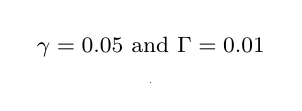
\begin{tikzpicture}[%
font=\footnotesize
]

\begin{axis}[%
width=0.951\figwidth,
height=\figheight,
at={(0\figwidth,0\figheight)},
scale only axis,
xmin=0,
xmax=3,
tick align=outside,
xlabel={Log-Moneyness},
xmajorgrids,
ymin=0,
ymax=5,
ylabel={Remaining Time},
ymajorgrids,
zmin=0,
zmax=20,
zlabel={Relative Increase},
zmajorgrids,
view={50}{40},
axis background/.style={fill=white},
title={$\gamma = 0.05$ and $\Gamma = 0.01$},
axis x line*=bottom,
axis y line*=left,
axis z line*=left
]

\addplot3[%
surf,
shader=flat corner,draw=black,z buffer=sort,colormap={mymap}{[1pt] rgb(0pt)=(0.2081,0.1663,0.5292); rgb(1pt)=(0.211624,0.189781,0.577676); rgb(2pt)=(0.212252,0.213771,0.626971); rgb(3pt)=(0.2081,0.2386,0.677086); rgb(4pt)=(0.195905,0.264457,0.7279); rgb(5pt)=(0.170729,0.291938,0.779248); rgb(6pt)=(0.125271,0.324243,0.830271); rgb(7pt)=(0.0591333,0.359833,0.868333); rgb(8pt)=(0.0116952,0.38751,0.881957); rgb(9pt)=(0.00595714,0.408614,0.882843); rgb(10pt)=(0.0165143,0.4266,0.878633); rgb(11pt)=(0.0328524,0.443043,0.871957); rgb(12pt)=(0.0498143,0.458571,0.864057); rgb(13pt)=(0.0629333,0.47369,0.855438); rgb(14pt)=(0.0722667,0.488667,0.8467); rgb(15pt)=(0.0779429,0.503986,0.838371); rgb(16pt)=(0.0793476,0.520024,0.831181); rgb(17pt)=(0.0749429,0.537543,0.826271); rgb(18pt)=(0.0640571,0.556986,0.823957); rgb(19pt)=(0.0487714,0.577224,0.822829); rgb(20pt)=(0.0343429,0.596581,0.819852); rgb(21pt)=(0.0265,0.6137,0.8135); rgb(22pt)=(0.0238905,0.628662,0.803762); rgb(23pt)=(0.0230905,0.641786,0.791267); rgb(24pt)=(0.0227714,0.653486,0.776757); rgb(25pt)=(0.0266619,0.664195,0.760719); rgb(26pt)=(0.0383714,0.674271,0.743552); rgb(27pt)=(0.0589714,0.683757,0.725386); rgb(28pt)=(0.0843,0.692833,0.706167); rgb(29pt)=(0.113295,0.7015,0.685857); rgb(30pt)=(0.145271,0.709757,0.664629); rgb(31pt)=(0.180133,0.717657,0.642433); rgb(32pt)=(0.217829,0.725043,0.619262); rgb(33pt)=(0.258643,0.731714,0.595429); rgb(34pt)=(0.302171,0.737605,0.571186); rgb(35pt)=(0.348167,0.742433,0.547267); rgb(36pt)=(0.395257,0.7459,0.524443); rgb(37pt)=(0.44201,0.748081,0.503314); rgb(38pt)=(0.487124,0.749062,0.483976); rgb(39pt)=(0.530029,0.749114,0.466114); rgb(40pt)=(0.570857,0.748519,0.44939); rgb(41pt)=(0.609852,0.747314,0.433686); rgb(42pt)=(0.6473,0.7456,0.4188); rgb(43pt)=(0.683419,0.743476,0.404433); rgb(44pt)=(0.71841,0.741133,0.390476); rgb(45pt)=(0.752486,0.7384,0.376814); rgb(46pt)=(0.785843,0.735567,0.363271); rgb(47pt)=(0.818505,0.732733,0.34979); rgb(48pt)=(0.850657,0.7299,0.336029); rgb(49pt)=(0.882433,0.727433,0.3217); rgb(50pt)=(0.913933,0.725786,0.306276); rgb(51pt)=(0.944957,0.726114,0.288643); rgb(52pt)=(0.973895,0.731395,0.266648); rgb(53pt)=(0.993771,0.745457,0.240348); rgb(54pt)=(0.999043,0.765314,0.216414); rgb(55pt)=(0.995533,0.786057,0.196652); rgb(56pt)=(0.988,0.8066,0.179367); rgb(57pt)=(0.978857,0.827143,0.163314); rgb(58pt)=(0.9697,0.848138,0.147452); rgb(59pt)=(0.962586,0.870514,0.1309); rgb(60pt)=(0.958871,0.8949,0.113243); rgb(61pt)=(0.959824,0.921833,0.0948381); rgb(62pt)=(0.9661,0.951443,0.0755333); rgb(63pt)=(0.9763,0.9831,0.0538)},mesh/rows=25]
table[row sep=crcr, point meta=\thisrow{c}] {%
%
x	y	z	c\\
0	0.01	2.03880318954621	2.03880318954621\\
0	0.111836734693878	6.69592840241886	6.69592840241886\\
0	0.213673469387755	8.8609434743905	8.8609434743905\\
0	0.315510204081633	10.2861865176267	10.2861865176267\\
0	0.41734693877551	11.3129998240506	11.3129998240506\\
0	0.519183673469388	12.0892406665137	12.0892406665137\\
0	0.621020408163265	12.6950579128353	12.6950579128353\\
0	0.722857142857143	13.1791712626296	13.1791712626296\\
0	0.82469387755102	13.5733654151918	13.5733654151918\\
0	0.926530612244898	13.8994091948017	13.8994091948017\\
0	1.02836734693878	14.1727556031593	14.1727556031593\\
0	1.13020408163265	14.4046829161444	14.4046829161444\\
0	1.23204081632653	14.603607909424	14.603607909424\\
0	1.33387755102041	14.7759282596328	14.7759282596328\\
0	1.43571428571429	14.9265825953534	14.9265825953534\\
0	1.53755102040816	15.059433902106	15.059433902106\\
0	1.63938775510204	15.1775385146179	15.1775385146179\\
0	1.74122448979592	15.2833388256283	15.2833388256283\\
0	1.8430612244898	15.3788038639446	15.3788038639446\\
0	1.94489795918367	15.4655334809344	15.4655334809344\\
0	2.04673469387755	15.5448366557039	15.5448366557039\\
0	2.14857142857143	15.617791088705	15.617791088705\\
0	2.25040816326531	15.685289067747	15.685289067747\\
0	2.35224489795918	15.7480731293531	15.7480731293531\\
0	2.45408163265306	15.8067640434897	15.8067640434897\\
0	2.55591836734694	15.8618829604288	15.8618829604288\\
0	2.65775510204082	15.9138690738389	15.9138690738389\\
0	2.75959183673469	15.9630938086454	15.9630938086454\\
0	2.86142857142857	16.0098722924769	16.0098722924769\\
0	2.96326530612245	16.0544726873411	16.0544726873411\\
0	3.06510204081633	16.0971238233916	16.0971238233916\\
0	3.1669387755102	16.1380214763788	16.1380214763788\\
0	3.26877551020408	16.1773335547659	16.1773335547659\\
0	3.37061224489796	16.2152044051004	16.2152044051004\\
0	3.47244897959184	16.2517584004477	16.2517584004477\\
0	3.57428571428571	16.287102942805	16.287102942805\\
0	3.67612244897959	16.3213309841586	16.3213309841586\\
0	3.77795918367347	16.3545231503346	16.3545231503346\\
0	3.87979591836735	16.3867495357033	16.3867495357033\\
0	3.98163265306122	16.4180712239355	16.4180712239355\\
0	4.0834693877551	16.4485415799743	16.4485415799743\\
0	4.18530612244898	16.4782073501392	16.4782073501392\\
0	4.28714285714286	16.5071096009002	16.5071096009002\\
0	4.38897959183674	16.5352845214374	16.5352845214374\\
0	4.49081632653061	16.562764110922	16.562764110922\\
0	4.59265306122449	16.5895767679922	16.5895767679922\\
0	4.69448979591837	16.61574779691	16.61574779691\\
0	4.79632653061224	16.6412998426844	16.6412998426844\\
0	4.89816326530612	16.6662532654711	16.6662532654711\\
0	5	16.69062646288	16.69062646288\\
0.125	0.01	0.0107194298990472	0.0107194298990472\\
0.125	0.111836734693878	2.29262852438333	2.29262852438333\\
0.125	0.213673469387755	4.26103604125503	4.26103604125503\\
0.125	0.315510204081633	5.72990445783214	5.72990445783214\\
0.125	0.41734693877551	6.86683596924776	6.86683596924776\\
0.125	0.519183673469388	7.77267367405898	7.77267367405898\\
0.125	0.621020408163265	8.51054154375529	8.51054154375529\\
0.125	0.722857142857143	9.12227940170954	9.12227940170954\\
0.125	0.82469387755102	9.63689066392033	9.63689066392033\\
0.125	0.926530612244898	10.0751881904375	10.0751881904375\\
0.125	1.02836734693878	10.4525220011769	10.4525220011769\\
0.125	1.13020408163265	10.7804682280945	10.7804682280945\\
0.125	1.23204081632653	11.0679204471935	11.0679204471935\\
0.125	1.33387755102041	11.3218197644407	11.3218197644407\\
0.125	1.43571428571429	11.5476574926833	11.5476574926833\\
0.125	1.53755102040816	11.749829758864	11.749829758864\\
0.125	1.63938775510204	11.9318929157782	11.9318929157782\\
0.125	1.74122448979592	12.0967508605655	12.0967508605655\\
0.125	1.8430612244898	12.2467946116762	12.2467946116762\\
0.125	1.94489795918367	12.3840077870884	12.3840077870884\\
0.125	2.04673469387755	12.5100473248494	12.5100473248494\\
0.125	2.14857142857143	12.6263059625628	12.6263059625628\\
0.125	2.25040816326531	12.7339610985922	12.7339610985922\\
0.125	2.35224489795918	12.8340123330511	12.8340123330511\\
0.125	2.45408163265306	12.9273173343392	12.9273173343392\\
0.125	2.55591836734694	13.0146061796201	13.0146061796201\\
0.125	2.65775510204082	13.0965115905565	13.0965115905565\\
0.125	2.75959183673469	13.1735799990254	13.1735799990254\\
0.125	2.86142857142857	13.2462858632893	13.2462858632893\\
0.125	2.96326530612245	13.3150426135759	13.3150426135759\\
0.125	3.06510204081633	13.380211705274	13.380211705274\\
0.125	3.1669387755102	13.4421102252556	13.4421102252556\\
0.125	3.26877551020408	13.5010171238143	13.5010171238143\\
0.125	3.37061224489796	13.5571785765481	13.5571785765481\\
0.125	3.47244897959184	13.6108124504741	13.6108124504741\\
0.125	3.57428571428571	13.6621120987551	13.6621120987551\\
0.125	3.67612244897959	13.7112495875494	13.7112495875494\\
0.125	3.77795918367347	13.7583784495122	13.7583784495122\\
0.125	3.87979591836735	13.8036360410738	13.8036360410738\\
0.125	3.98163265306122	13.8471455667168	13.8471455667168\\
0.125	4.0834693877551	13.8890178223257	13.8890178223257\\
0.125	4.18530612244898	13.9293527006798	13.9293527006798\\
0.125	4.28714285714286	13.9682404948713	13.9682404948713\\
0.125	4.38897959183674	14.0057630294881	14.0057630294881\\
0.125	4.49081632653061	14.0419946445437	14.0419946445437\\
0.125	4.59265306122449	14.0770030114927	14.0770030114927\\
0.125	4.69448979591837	14.1108500597706	14.1108500597706\\
0.125	4.79632653061224	14.1435923530339	14.1435923530339\\
0.125	4.89816326530612	14.1752818563703	14.1752818563703\\
0.125	5	14.2059663726667	14.2059663726667\\
0.25	0.01	3.02554867109697e-07	3.02554867109697e-07\\
0.25	0.111836734693878	0.538987396497311	0.538987396497311\\
0.25	0.213673469387755	1.70128321703374	1.70128321703374\\
0.25	0.315510204081633	2.82621729895949	2.82621729895949\\
0.25	0.41734693877551	3.81102326155211	3.81102326155211\\
0.25	0.519183673469388	4.65775195411126	4.65775195411126\\
0.25	0.621020408163265	5.38571639645315	5.38571639645315\\
0.25	0.722857142857143	6.01475669756002	6.01475669756002\\
0.25	0.82469387755102	6.56189445406548	6.56189445406548\\
0.25	0.926530612244898	7.04104886009791	7.04104886009791\\
0.25	1.02836734693878	7.46345374931528	7.46345374931528\\
0.25	1.13020408163265	7.83816840951684	7.83816840951684\\
0.25	1.23204081632653	8.17252855052991	8.17252855052991\\
0.25	1.33387755102041	8.47251049712894	8.47251049712894\\
0.25	1.43571428571429	8.74301630825928	8.74301630825928\\
0.25	1.53755102040816	8.98809479259066	8.98809479259066\\
0.25	1.63938775510204	9.21111270466073	9.21111270466073\\
0.25	1.74122448979592	9.4148878211462	9.4148878211462\\
0.25	1.8430612244898	9.601792964697	9.601792964697\\
0.25	1.94489795918367	9.77383784999905	9.77383784999905\\
0.25	2.04673469387755	9.93273392825189	9.93273392825189\\
0.25	2.14857142857143	10.0799461011624	10.0799461011624\\
0.25	2.25040816326531	10.2167342788385	10.2167342788385\\
0.25	2.35224489795918	10.3441869606521	10.3441869606521\\
0.25	2.45408163265306	10.4632485582489	10.4632485582489\\
0.25	2.55591836734694	10.5747417808161	10.5747417808161\\
0.25	2.65775510204082	10.6793860110296	10.6793860110296\\
0.25	2.75959183673469	10.7778125675806	10.7778125675806\\
0.25	2.86142857142857	10.8705773563007	10.8705773563007\\
0.25	2.96326530612245	10.9581715409233	10.9581715409233\\
0.25	3.06510204081633	11.0410303448418	11.0410303448418\\
0.25	3.1669387755102	11.1195406187568	11.1195406187568\\
0.25	3.26877551020408	11.1940471880998	11.1940471880998\\
0.25	3.37061224489796	11.2648582622911	11.2648582622911\\
0.25	3.47244897959184	11.3322500522528	11.3322500522528\\
0.25	3.57428571428571	11.3964707260869	11.3964707260869\\
0.25	3.67612244897959	11.4577438092239	11.4577438092239\\
0.25	3.77795918367347	11.5162711164332	11.5162711164332\\
0.25	3.87979591836735	11.5722352878511	11.5722352878511\\
0.25	3.98163265306122	11.6258019888562	11.6258019888562\\
0.25	4.0834693877551	11.6771218236044	11.6771218236044\\
0.25	4.18530612244898	11.7263320038499	11.7263320038499\\
0.25	4.28714285714286	11.7735578079769	11.7735578079769\\
0.25	4.38897959183674	11.8189138596397	11.8189138596397\\
0.25	4.49081632653061	11.8625052508489	11.8625052508489\\
0.25	4.59265306122449	11.9044285305531	11.9044285305531\\
0.25	4.69448979591837	11.9447725766144	11.9447725766144\\
0.25	4.79632653061224	11.9836193246591	11.9836193246591\\
0.25	4.89816326530612	12.0210446593395	12.0210446593395\\
0.25	5	12.057118601767	12.057118601767\\
0.375	0.01	2.47232115763359e-14	2.47232115763359e-14\\
0.375	0.111836734693878	0.0826403598090983	0.0826403598090983\\
0.375	0.213673469387755	0.551346453489448	0.551346453489448\\
0.375	0.315510204081633	1.21762197274726	1.21762197274726\\
0.375	0.41734693877551	1.91574207183352	1.91574207183352\\
0.375	0.519183673469388	2.5831068208131	2.5831068208131\\
0.375	0.621020408163265	3.19933960046873	3.19933960046873\\
0.375	0.722857142857143	3.76039462396615	3.76039462396615\\
0.375	0.82469387755102	4.26851289317224	4.26851289317224\\
0.375	0.926530612244898	4.72816859564129	4.72816859564129\\
0.375	1.02836734693878	5.14438364311698	5.14438364311698\\
0.375	1.13020408163265	5.52203119597596	5.52203119597596\\
0.375	1.23204081632653	5.86556880415044	5.86556880415044\\
0.375	1.33387755102041	6.17896141145011	6.17896141145011\\
0.375	1.43571428571429	6.46568712423698	6.46568712423698\\
0.375	1.53755102040816	6.72877664774985	6.72877664774985\\
0.375	1.63938775510204	6.97086370589394	6.97086370589394\\
0.375	1.74122448979592	7.1942361427958	7.1942361427958\\
0.375	1.8430612244898	7.4008833084079	7.4008833084079\\
0.375	1.94489795918367	7.5925381520172	7.5925381520172\\
0.375	2.04673469387755	7.7707137714242	7.7707137714242\\
0.375	2.14857142857143	7.9367347536193	7.9367347536193\\
0.375	2.25040816326531	8.09176386962199	8.09176386962199\\
0.375	2.35224489795918	8.23682473887708	8.23682473887708\\
0.375	2.45408163265306	8.37282105137868	8.37282105137868\\
0.375	2.55591836734694	8.50055287576402	8.50055287576402\\
0.375	2.65775510204082	8.62073051228113	8.62073051228113\\
0.375	2.75959183673469	8.73398628178988	8.73398628178988\\
0.375	2.86142857142857	8.84088458052876	8.84088458052876\\
0.375	2.96326530612245	8.94193047683079	8.94193047683079\\
0.375	3.06510204081633	9.03757708033732	9.03757708033732\\
0.375	3.1669387755102	9.12823187588928	9.12823187588928\\
0.375	3.26877551020408	9.21426218227413	9.21426218227413\\
0.375	3.37061224489796	9.29599986944064	9.29599986944064\\
0.375	3.47244897959184	9.37374544579114	9.37374544579114\\
0.375	3.57428571428571	9.44777160895449	9.44777160895449\\
0.375	3.67612244897959	9.51832633837463	9.51832633837463\\
0.375	3.77795918367347	9.58563559556622	9.58563559556622\\
0.375	3.87979591836735	9.64990568753298	9.64990568753298\\
0.375	3.98163265306122	9.71132534023597	9.71132534023597\\
0.375	4.0834693877551	9.77006752183052	9.77006752183052\\
0.375	4.18530612244898	9.82629104940488	9.82629104940488\\
0.375	4.28714285714286	9.88014200794613	9.88014200794613\\
0.375	4.38897959183674	9.93175500766385	9.93175500766385\\
0.375	4.49081632653061	9.9812542923083	9.9812542923083\\
0.375	4.59265306122449	10.0287547342337	10.0287547342337\\
0.375	4.69448979591837	10.0743627120769	10.0743627120769\\
0.375	4.79632653061224	10.1181768962927	10.1181768962927\\
0.375	4.89816326530612	10.1602889503879	10.1602889503879\\
0.375	5	10.2007841583159	10.2007841583159\\
0.5	0.01	4.77299678866057e-24	4.77299678866057e-24\\
0.5	0.111836734693878	0.00796919311511591	0.00796919311511591\\
0.5	0.213673469387755	0.142455085914167	0.142455085914167\\
0.5	0.315510204081633	0.45304380739868	0.45304380739868\\
0.5	0.41734693877551	0.865219773501635	0.865219773501635\\
0.5	0.519183673469388	1.31757315551536	1.31757315551536\\
0.5	0.621020408163265	1.77518905652915	1.77518905652915\\
0.5	0.722857142857143	2.21999858755654	2.21999858755654\\
0.5	0.82469387755102	2.64331124483295	2.64331124483295\\
0.5	0.926530612244898	3.04151501149199	3.04151501149199\\
0.5	1.02836734693878	3.413718366368	3.413718366368\\
0.5	1.13020408163265	3.76045961506731	3.76045961506731\\
0.5	1.23204081632653	4.08299502639142	4.08299502639142\\
0.5	1.33387755102041	4.38290402871435	4.38290402871435\\
0.5	1.43571428571429	4.66187074397452	4.66187074397452\\
0.5	1.53755102040816	4.92156498041436	4.92156498041436\\
0.5	1.63938775510204	5.1635798926706	5.1635798926706\\
0.5	1.74122448979592	5.38940206815663	5.38940206815663\\
0.5	1.8430612244898	5.60040010041753	5.60040010041753\\
0.5	1.94489795918367	5.7978235418106	5.7978235418106\\
0.5	2.04673469387755	5.98280748594457	5.98280748594457\\
0.5	2.14857142857143	6.1563799922559	6.1563799922559\\
0.5	2.25040816326531	6.3194707247422	6.3194707247422\\
0.5	2.35224489795918	6.47291986806759	6.47291986806759\\
0.5	2.45408163265306	6.61748679816266	6.61748679816266\\
0.5	2.55591836734694	6.75385823234265	6.75385823234265\\
0.5	2.65775510204082	6.8826557315993	6.8826557315993\\
0.5	2.75959183673469	7.00444251442024	7.00444251442024\\
0.5	2.86142857142857	7.11972959105111	7.11972959105111\\
0.5	2.96326530612245	7.22898125406407	7.22898125406407\\
0.5	3.06510204081633	7.33261997435774	7.33261997435774\\
0.5	3.1669387755102	7.43103075679885	7.43103075679885\\
0.5	3.26877551020408	7.52456501003038	7.52456501003038\\
0.5	3.37061224489796	7.6135439826204	7.6135439826204\\
0.5	3.47244897959184	7.69826181399849	7.69826181399849\\
0.5	3.57428571428571	7.77898824430706	7.77898824430706\\
0.5	3.67612244897959	7.85597102284615	7.85597102284615\\
0.5	3.77795918367347	7.92943805047914	7.92943805047914\\
0.5	3.87979591836735	7.99959928733482	7.99959928733482\\
0.5	3.98163265306122	8.06664845345563	8.06664845345563\\
0.5	4.0834693877551	8.13076454672345	8.13076454672345\\
0.5	4.18530612244898	8.19211319943702	8.19211319943702\\
0.5	4.28714285714286	8.25084789229945	8.25084789229945\\
0.5	4.38897959183674	8.30711104227108	8.30711104227108\\
0.5	4.49081632653061	8.36103497872387	8.36103497872387\\
0.5	4.59265306122449	8.41274282056529	8.41274282056529\\
0.5	4.69448979591837	8.46234926545554	8.46234926545554\\
0.5	4.79632653061224	8.50996130089315	8.50996130089315\\
0.5	4.89816326530612	8.55567884576701	8.55567884576701\\
0.5	5	8.59959532994542	8.59959532994542\\
0.625	0.01	2.00269367534608e-36	2.00269367534608e-36\\
0.625	0.111836734693878	0.000471410628550751	0.000471410628550751\\
0.625	0.213673469387755	0.0289430104287286	0.0289430104287286\\
0.625	0.315510204081633	0.144238335927612	0.144238335927612\\
0.625	0.41734693877551	0.348701560076033	0.348701560076033\\
0.625	0.519183673469388	0.614834236280209	0.614834236280209\\
0.625	0.621020408163265	0.916023074426006	0.916023074426006\\
0.625	0.722857142857143	1.23306640710524	1.23306640710524\\
0.625	0.82469387755102	1.55337674932524	1.55337674932524\\
0.625	0.926530612244898	1.86909097071294	1.86909097071294\\
0.625	1.02836734693878	2.17549564813142	2.17549564813142\\
0.625	1.13020408163265	2.46992258217855	2.46992258217855\\
0.625	1.23204081632653	2.75101504484162	2.75101504484162\\
0.625	1.33387755102041	3.01824915767039	3.01824915767039\\
0.625	1.43571428571429	3.27162322213489	3.27162322213489\\
0.625	1.53755102040816	3.51145608398489	3.51145608398489\\
0.625	1.63938775510204	3.73825615914596	3.73825615914596\\
0.625	1.74122448979592	3.95263640443065	3.95263640443065\\
0.625	1.8430612244898	4.15525931372946	4.15525931372946\\
0.625	1.94489795918367	4.34680163738004	4.34680163738004\\
0.625	2.04673469387755	4.52793211206616	4.52793211206616\\
0.625	2.14857142857143	4.69929779525311	4.69929779525311\\
0.625	2.25040816326531	4.86151609163152	4.86151609163152\\
0.625	2.35224489795918	5.015170534069	5.015170534069\\
0.625	2.45408163265306	5.16080902345898	5.16080902345898\\
0.625	2.55591836734694	5.29894365779993	5.29894365779993\\
0.625	2.65775510204082	5.4300515655491	5.4300515655491\\
0.625	2.75959183673469	5.55457634982958	5.55457634982958\\
0.625	2.86142857142857	5.67292987962197	5.67292987962197\\
0.625	2.96326530612245	5.78549425207498	5.78549425207498\\
0.625	3.06510204081633	5.89262381002683	5.89262381002683\\
0.625	3.1669387755102	5.99464713973554	5.99464713973554\\
0.625	3.26877551020408	6.0918690017144	6.0918690017144\\
0.625	3.37061224489796	6.1845721665438	6.1845721665438\\
0.625	3.47244897959184	6.27301914036398	6.27301914036398\\
0.625	3.57428571428571	6.35745377335102	6.35745377335102\\
0.625	3.67612244897959	6.43810275015022	6.43810275015022\\
0.625	3.77795918367347	6.51517696489553	6.51517696489553\\
0.625	3.87979591836735	6.58887278570852	6.58887278570852\\
0.625	3.98163265306122	6.65937321488406	6.65937321488406\\
0.625	4.0834693877551	6.72684895163771	6.72684895163771\\
0.625	4.18530612244898	6.79145936452403	6.79145936452403\\
0.625	4.28714285714286	6.85335338058492	6.85335338058492\\
0.625	4.38897959183674	6.91267029805435	6.91267029805435\\
0.625	4.49081632653061	6.96954052910365	6.96954052910365\\
0.625	4.59265306122449	7.02408627870744	7.02408627870744\\
0.625	4.69448979591837	7.07642216527821	7.07642216527821\\
0.625	4.79632653061224	7.12665578828005	7.12665578828005\\
0.625	4.89816326530612	7.1748882476034	7.1748882476034\\
0.625	5	7.22121461907176	7.22121461907176\\
0.75	0.01	1.752670608309e-51	1.752670608309e-51\\
0.75	0.111836734693878	1.68139993851589e-05	1.68139993851589e-05\\
0.75	0.213673469387755	0.00457569160139879	0.00457569160139879\\
0.75	0.315510204081633	0.0390047553467661	0.0390047553467661\\
0.75	0.41734693877551	0.124700492756297	0.124700492756297\\
0.75	0.519183673469388	0.261293081189028	0.261293081189028\\
0.75	0.621020408163265	0.43794052870176	0.43794052870176\\
0.75	0.722857142857143	0.642310977015885	0.642310977015885\\
0.75	0.82469387755102	0.863881336396762	0.863881336396762\\
0.75	0.926530612244898	1.09457886527776	1.09457886527776\\
0.75	1.02836734693878	1.32852421396216	1.32852421396216\\
0.75	1.13020408163265	1.5615698758581	1.5615698758581\\
0.75	1.23204081632653	1.79086482125778	1.79086482125778\\
0.75	1.33387755102041	2.01450373309781	2.01450373309781\\
0.75	1.43571428571429	2.23126156505291	2.23126156505291\\
0.75	1.53755102040816	2.44039833642282	2.44039833642282\\
0.75	1.63938775510204	2.64151750975451	2.64151750975451\\
0.75	1.74122448979592	2.83446387779738	2.83446387779738\\
0.75	1.8430612244898	3.01925012638117	3.01925012638117\\
0.75	1.94489795918367	3.1960040698355	3.1960040698355\\
0.75	2.04673469387755	3.36493075893682	3.36493075893682\\
0.75	2.14857142857143	3.52628529368378	3.52628529368378\\
0.75	2.25040816326531	3.68035335439849	3.68035335439849\\
0.75	2.35224489795918	3.82743731019601	3.82743731019601\\
0.75	2.45408163265306	3.9678463666743	3.9678463666743\\
0.75	2.55591836734694	4.10188964432088	4.10188964432088\\
0.75	2.65775510204082	4.22987138594862	4.22987138594862\\
0.75	2.75959183673469	4.35208771127752	4.35208771127752\\
0.75	2.86142857142857	4.46882449486184	4.46882449486184\\
0.75	2.96326530612245	4.58035605773406	4.58035605773406\\
0.75	3.06510204081633	4.68694444594917	4.68694444594917\\
0.75	3.1669387755102	4.7888391295331	4.7888391295331\\
0.75	3.26877551020408	4.88627699945073	4.88627699945073\\
0.75	3.37061224489796	4.9794825725884	4.9794825725884\\
0.75	3.47244897959184	5.06866833859232	5.06866833859232\\
0.75	3.57428571428571	5.15403520001755	5.15403520001755\\
0.75	3.67612244897959	5.23577297028358	5.23577297028358\\
0.75	3.77795918367347	5.3140609036064	5.3140609036064\\
0.75	3.87979591836735	5.38906823826132	5.38906823826132\\
0.75	3.98163265306122	5.46095473986952	5.46095473986952\\
0.75	4.0834693877551	5.5298712353669	5.5298712353669\\
0.75	4.18530612244898	5.59596013125494	5.59596013125494\\
0.75	4.28714285714286	5.65935591190983	5.65935591190983\\
0.75	4.38897959183674	5.72018561532931	5.72018561532931\\
0.75	4.49081632653061	5.77856928487121	5.77856928487121\\
0.75	4.59265306122449	5.83462039638985	5.83462039638985\\
0.75	4.69448979591837	5.88844626078832	5.88844626078832\\
0.75	4.79632653061224	5.94014840243529	5.94014840243529\\
0.75	4.89816326530612	5.9898229141911	5.9898229141911\\
0.75	5	6.03756078998367	6.03756078998367\\
0.875	0.01	3.1263090256729e-69	3.1263090256729e-69\\
0.875	0.111836734693878	3.57271243466546e-07	3.57271243466546e-07\\
0.875	0.213673469387755	0.000558396440006046	0.000558396440006046\\
0.875	0.315510204081633	0.00890603034378278	0.00890603034378278\\
0.875	0.41734693877551	0.0393868910376378	0.0393868910376378\\
0.875	0.519183673469388	0.100746820955289	0.100746820955289\\
0.875	0.621020408163265	0.193363992057449	0.193363992057449\\
0.875	0.722857142857143	0.312913949072435	0.312913949072435\\
0.875	0.82469387755102	0.453546585554672	0.453546585554672\\
0.875	0.926530612244898	0.609532098442136	0.609532098442136\\
0.875	1.02836734693878	0.77590902455474	0.77590902455474\\
0.875	1.13020408163265	0.94863782027092	0.94863782027092\\
0.875	1.23204081632653	1.12454506059041	1.12454506059041\\
0.875	1.33387755102041	1.30119626159179	1.30119626159179\\
0.875	1.43571428571429	1.47675802265998	1.47675802265998\\
0.875	1.53755102040816	1.64987320798524	1.64987320798524\\
0.875	1.63938775510204	1.81955624026398	1.81955624026398\\
0.875	1.74122448979592	1.98510859881891	1.98510859881891\\
0.875	1.8430612244898	2.14605205466694	2.14605205466694\\
0.875	1.94489795918367	2.30207654949877	2.30207654949877\\
0.875	2.04673469387755	2.45299978342322	2.45299978342322\\
0.875	2.14857142857143	2.59873600006663	2.59873600006663\\
0.875	2.25040816326531	2.73927192510494	2.73927192510494\\
0.875	2.35224489795918	2.87464823898069	2.87464823898069\\
0.875	2.45408163265306	3.00494532020585	3.00494532020585\\
0.875	2.55591836734694	3.13027228142216	3.13027228142216\\
0.875	2.65775510204082	3.25075854482331	3.25075854482331\\
0.875	2.75959183673469	3.36654737753258	3.36654737753258\\
0.875	2.86142857142857	3.47779094144388	3.47779094144388\\
0.875	2.96326530612245	3.58464651472852	3.58464651472852\\
0.875	3.06510204081633	3.68727362085488	3.68727362085488\\
0.875	3.1669387755102	3.78583186120046	3.78583186120046\\
0.875	3.26877551020408	3.88047929351741	3.88047929351741\\
0.875	3.37061224489796	3.97137123398108	3.97137123398108\\
0.875	3.47244897959184	4.05865938784983	4.05865938784983\\
0.875	3.57428571428571	4.14249123482432	4.14249123482432\\
0.875	3.67612244897959	4.22300961148266	4.22300961148266\\
0.875	3.77795918367347	4.30035244579625	4.30035244579625\\
0.875	3.87979591836735	4.37465260854732	4.37465260854732\\
0.875	3.98163265306122	4.44603785411721	4.44603785411721\\
0.875	4.0834693877551	4.51463082908785	4.51463082908785\\
0.875	4.18530612244898	4.58054913177312	4.58054913177312\\
0.875	4.28714285714286	4.64390540946269	4.64390540946269\\
0.875	4.38897959183674	4.70480748304074	4.70480748304074\\
0.875	4.49081632653061	4.7633584909076	4.7633584909076\\
0.875	4.59265306122449	4.81965704591689	4.81965704591689\\
0.875	4.69448979591837	4.87379740044892	4.87379740044892\\
0.875	4.79632653061224	4.92586961585084	4.92586961585084\\
0.875	4.89816326530612	4.97595973335153	4.97595973335153\\
0.875	5	5.02414994425069	5.02414994425069\\
1	0.01	1.12063209457396e-89	1.12063209457396e-89\\
1	0.111836734693878	4.48377411198789e-09	4.48377411198789e-09\\
1	0.213673469387755	5.22808212603453e-05	5.22808212603453e-05\\
1	0.315510204081633	0.00170896437087865	0.00170896437087865\\
1	0.41734693877551	0.0109458300354403	0.0109458300354403\\
1	0.519183673469388	0.0351304210957638	0.0351304210957638\\
1	0.621020408163265	0.0786321312487697	0.0786321312487697\\
1	0.722857142857143	0.142228554578698	0.142228554578698\\
1	0.82469387755102	0.224315013913293	0.224315013913293\\
1	0.926530612244898	0.322144126429393	0.322144126429393\\
1	1.02836734693878	0.432642593474647	0.432642593474647\\
1	1.13020408163265	0.55285377917609	0.55285377917609\\
1	1.23204081632653	0.680139234388953	0.680139234388953\\
1	1.33387755102041	0.812244663914662	0.812244663914662\\
1	1.43571428571429	0.947296718138405	0.947296718138405\\
1	1.53755102040816	1.08376841251578	1.08376841251578\\
1	1.63938775510204	1.22043337216554	1.22043337216554\\
1	1.74122448979592	1.35631904110695	1.35631904110695\\
1	1.8430612244898	1.49066350419582	1.49066350419582\\
1	1.94489795918367	1.62287768396021	1.62287768396021\\
1	2.04673469387755	1.75251322677937	1.75251322677937\\
1	2.14857142857143	1.87923571899163	1.87923571899163\\
1	2.25040816326531	2.00280260507788	2.00280260507788\\
1	2.35224489795918	2.12304511613263	2.12304511613263\\
1	2.45408163265306	2.23985354963911	2.23985354963911\\
1	2.55591836734694	2.35316531451145	2.35316531451145\\
1	2.65775510204082	2.46295523967799	2.46295523967799\\
1	2.75959183673469	2.5692277263265	2.5692277263265\\
1	2.86142857142857	2.67201039737434	2.67201039737434\\
1	2.96326530612245	2.77134896087245	2.77134896087245\\
1	3.06510204081633	2.86730305698286	2.86730305698286\\
1	3.1669387755102	2.95994290184057	2.95994290184057\\
1	3.26877551020408	3.04934657728077	3.04934657728077\\
1	3.37061224489796	3.13559784436129	3.13559784436129\\
1	3.47244897959184	3.21878438201297	3.21878438201297\\
1	3.57428571428571	3.29899637102694	3.29899637102694\\
1	3.67612244897959	3.37632535879719	3.37632535879719\\
1	3.77795918367347	3.45086335248964	3.45086335248964\\
1	3.87979591836735	3.52270209818262	3.52270209818262\\
1	3.98163265306122	3.59193251148853	3.59193251148853\\
1	4.0834693877551	3.65864423159701	3.65864423159701\\
1	4.18530612244898	3.72292527588	3.72292527588\\
1	4.28714285714286	3.78486177641024	3.78486177641024\\
1	4.38897959183674	3.84453778315967	3.84453778315967\\
1	4.49081632653061	3.90203512141935	3.90203512141935\\
1	4.59265306122449	3.95743329324007	3.95743329324007\\
1	4.69448979591837	4.01080941453356	4.01080941453356\\
1	4.79632653061224	4.06223818097665	4.06223818097665\\
1	4.89816326530612	4.11179185708952	4.11179185708952\\
1	5	4.15954028386549	4.15954028386549\\
1.125	0.01	7.99763070229431e-113	7.99763070229431e-113\\
1.125	0.111836734693878	3.3027744901111e-11	3.3027744901111e-11\\
1.125	0.213673469387755	3.73768296088946e-06	3.73768296088946e-06\\
1.125	0.315510204081633	0.000274552313016516	0.000274552313016516\\
1.125	0.41734693877551	0.00266808575386372	0.00266808575386372\\
1.125	0.519183673469388	0.0110490518929728	0.0110490518929728\\
1.125	0.621020408163265	0.0293818886603229	0.0293818886603229\\
1.125	0.722857142857143	0.0601919498468953	0.0601919498468953\\
1.125	0.82469387755102	0.104318934023723	0.104318934023723\\
1.125	0.926530612244898	0.161317878352752	0.161317878352752\\
1.125	1.02836734693878	0.22996466750566	0.22996466750566\\
1.125	1.13020408163265	0.30865891326323	0.30865891326323\\
1.125	1.23204081632653	0.39569203430866	0.39569203430866\\
1.125	1.33387755102041	0.489406055918377	0.489406055918377\\
1.125	1.43571428571429	0.588277272611923	0.588277272611923\\
1.125	1.53755102040816	0.690952632921261	0.690952632921261\\
1.125	1.63938775510204	0.796258274271671	0.796258274271671\\
1.125	1.74122448979592	0.903192747788869	0.903192747788869\\
1.125	1.8430612244898	1.01091263919285	1.01091263919285\\
1.125	1.94489795918367	1.11871513401856	1.11871513401856\\
1.125	2.04673469387755	1.22602009607198	1.22602009607198\\
1.125	2.14857142857143	1.33235302319458	1.33235302319458\\
1.125	2.25040816326531	1.43732952984093	1.43732952984093\\
1.125	2.35224489795918	1.54064159443259	1.54064159443259\\
1.125	2.45408163265306	1.64204558182579	1.64204558182579\\
1.125	2.55591836734694	1.74135193332171	1.74135193332171\\
1.125	2.65775510204082	1.83841636288491	1.83841636288491\\
1.125	2.75959183673469	1.93313238095007	1.93313238095007\\
1.125	2.86142857142857	2.02542496978534	2.02542496978534\\
1.125	2.96326530612245	2.11524524701751	2.11524524701751\\
1.125	3.06510204081633	2.20256597090727	2.20256597090727\\
1.125	3.1669387755102	2.28737775908037	2.28737775908037\\
1.125	3.26877551020408	2.36968590994628	2.36968590994628\\
1.125	3.37061224489796	2.44950773212279	2.44950773212279\\
1.125	3.47244897959184	2.52687030148869	2.52687030148869\\
1.125	3.57428571428571	2.60180857794978	2.60180857794978\\
1.125	3.67612244897959	2.67436382471272	2.67436382471272\\
1.125	3.77795918367347	2.74458228197974	2.74458228197974\\
1.125	3.87979591836735	2.81251405468973	2.81251405468973\\
1.125	3.98163265306122	2.87821218042583	2.87821218042583\\
1.125	4.0834693877551	2.94173184906321	2.94173184906321\\
1.125	4.18530612244898	3.00312975029947	3.00312975029947\\
1.125	4.28714285714286	3.06246352903562	3.06246352903562\\
1.125	4.38897959183674	3.11979133177437	3.11979133177437\\
1.125	4.49081632653061	3.17517142987979	3.17517142987979\\
1.125	4.59265306122449	3.2286619077813	3.2286619077813\\
1.125	4.69448979591837	3.28032040608009	3.28032040608009\\
1.125	4.79632653061224	3.33020391108665	3.33020391108665\\
1.125	4.89816326530612	3.37836858363536	3.37836858363536\\
1.125	5	3.42486962112768	3.42486962112768\\
1.25	0.01	1.12912615955239e-138	1.12912615955239e-138\\
1.25	0.111836734693878	1.4212378555905e-13	1.4212378555905e-13\\
1.25	0.213673469387755	2.03291558308715e-07	2.03291558308715e-07\\
1.25	0.315510204081633	3.68163794826603e-05	3.68163794826603e-05\\
1.25	0.41734693877551	0.000568965494258423	0.000568965494258423\\
1.25	0.519183673469388	0.00312741706597636	0.00312741706597636\\
1.25	0.621020408163265	0.0100683470940669	0.0100683470940669\\
1.25	0.722857142857143	0.0236762820437491	0.0236762820437491\\
1.25	0.82469387755102	0.045545221593522	0.045545221593522\\
1.25	0.926530612244898	0.076429284773914	0.076429284773914\\
1.25	1.02836734693878	0.11636506626482	0.11636506626482\\
1.25	1.13020408163265	0.164878697831223	0.164878697831223\\
1.25	1.23204081632653	0.221182038083305	0.221182038083305\\
1.25	1.33387755102041	0.284325555438105	0.284325555438105\\
1.25	1.43571428571429	0.353305347446568	0.353305347446568\\
1.25	1.53755102040816	0.42713233875776	0.42713233875776\\
1.25	1.63938775510204	0.504873591118792	0.504873591118792\\
1.25	1.74122448979592	0.585674367710666	0.585674367710666\\
1.25	1.8430612244898	0.668767548022985	0.668767548022985\\
1.25	1.94489795918367	0.753475095844266	0.753475095844266\\
1.25	2.04673469387755	0.839204792581772	0.839204792581772\\
1.25	2.14857142857143	0.925444361635869	0.925444361635869\\
1.25	2.25040816326531	1.01175435138679	1.01175435138679\\
1.25	2.35224489795918	1.09776063017	1.09776063017\\
1.25	2.45408163265306	1.1831470052437	1.1831470052437\\
1.25	2.55591836734694	1.26764825527102	1.26764825527102\\
1.25	2.65775510204082	1.35104372358193	1.35104372358193\\
1.25	2.75959183673469	1.43315153057408	1.43315153057408\\
1.25	2.86142857142857	1.51382340974889	1.51382340974889\\
1.25	2.96326530612245	1.5929401407496	1.5929401407496\\
1.25	3.06510204081633	1.67040753617801	1.67040753617801\\
1.25	3.1669387755102	1.74615293150781	1.74615293150781\\
1.25	3.26877551020408	1.82012212554133	1.82012212554133\\
1.25	3.37061224489796	1.89227672027783	1.89227672027783\\
1.25	3.47244897959184	1.96259181229805	1.96259181229805\\
1.25	3.57428571428571	2.03105399189272	2.03105399189272\\
1.25	3.67612244897959	2.09765961059436	2.09765961059436\\
1.25	3.77795918367347	2.16241328216839	2.16241328216839\\
1.25	3.87979591836735	2.22532658628551	2.22532658628551\\
1.25	3.98163265306122	2.28641694793076	2.28641694793076\\
1.25	4.0834693877551	2.34570666906575	2.34570666906575\\
1.25	4.18530612244898	2.40322209214086	2.40322209214086\\
1.25	4.28714285714286	2.45899287777112	2.45899287777112\\
1.25	4.38897959183674	2.51305138126767	2.51305138126767\\
1.25	4.49081632653061	2.56543211478808	2.56543211478808\\
1.25	4.59265306122449	2.6161712836662	2.6161712836662\\
1.25	4.69448979591837	2.66530638703752	2.66530638703752\\
1.25	4.79632653061224	2.71287587421936	2.71287587421936\\
1.25	4.89816326530612	2.75891884946361	2.75891884946361\\
1.25	5	2.80347481869873	2.80347481869873\\
1.375	0.01	3.1390990579779e-167	3.1390990579779e-167\\
1.375	0.111836734693878	3.56004806200561e-16	3.56004806200561e-16\\
1.375	0.213673469387755	8.38737986827723e-09	8.38737986827723e-09\\
1.375	0.315510204081633	4.1106576118842e-06	4.1106576118842e-06\\
1.375	0.41734693877551	0.000105921001871643	0.000105921001871643\\
1.375	0.519183673469388	0.000795153589685543	0.000795153589685543\\
1.375	0.621020408163265	0.00315869406370304	0.00315869406370304\\
1.375	0.722857142857143	0.00864279206565122	0.00864279206565122\\
1.375	0.82469387755102	0.0186421797036751	0.0186421797036751\\
1.375	0.926530612244898	0.034215993670321	0.034215993670321\\
1.375	1.02836734693878	0.0559887976217451	0.0559887976217451\\
1.375	1.13020408163265	0.0841761752055259	0.0841761752055259\\
1.375	1.23204081632653	0.118666141208649	0.118666141208649\\
1.375	1.33387755102041	0.15911225359078	0.15911225359078\\
1.375	1.43571428571429	0.205017098973073	0.205017098973073\\
1.375	1.53755102040816	0.255798815891264	0.255798815891264\\
1.375	1.63938775510204	0.310840295592106	0.310840295592106\\
1.375	1.74122448979592	0.36952352194446	0.36952352194446\\
1.375	1.8430612244898	0.431252233907242	0.431252233907242\\
1.375	1.94489795918367	0.495465897023229	0.495465897023229\\
1.375	2.04673469387755	0.561647455618992	0.561647455618992\\
1.375	2.14857142857143	0.629326779821282	0.629326779821282\\
1.375	2.25040816326531	0.698081229799826	0.698081229799826\\
1.375	2.35224489795918	0.767534364159048	0.767534364159048\\
1.375	2.45408163265306	0.837353517165921	0.837353517165921\\
1.375	2.55591836734694	0.907246745833931	0.907246745833931\\
1.375	2.65775510204082	0.976959485988394	0.976959485988394\\
1.375	2.75959183673469	1.0462711412056	1.0462711412056\\
1.375	2.86142857142857	1.114991747647	1.114991747647\\
1.375	2.96326530612245	1.18295880180458	1.18295880180458\\
1.375	3.06510204081633	1.25003429993409	1.25003429993409\\
1.375	3.1669387755102	1.3161020122759	1.3161020122759\\
1.375	3.26877551020408	1.38106499828995	1.38106499828995\\
1.375	3.37061224489796	1.44484335837255	1.44484335837255\\
1.375	3.47244897959184	1.50737221096924	1.50737221096924\\
1.375	3.57428571428571	1.5685998803036	1.5685998803036\\
1.375	3.67612244897959	1.62848627816286	1.62848627816286\\
1.375	3.77795918367347	1.68700146265932	1.68700146265932\\
1.375	3.87979591836735	1.74412435716645	1.74412435716645\\
1.375	3.98163265306122	1.79984161339856	1.79984161339856\\
1.375	4.0834693877551	1.85414660364931	1.85414660364931\\
1.375	4.18530612244898	1.90703852838605	1.90703852838605\\
1.375	4.28714285714286	1.9585216266205	1.9585216266205\\
1.375	4.38897959183674	2.00860447768092	2.00860447768092\\
1.375	4.49081632653061	2.05729938416197	2.05729938416197\\
1.375	4.59265306122449	2.10462182690346	2.10462182690346\\
1.375	4.69448979591837	2.15058998383893	2.15058998383893\\
1.375	4.79632653061224	2.19522430545649	2.19522430545649\\
1.375	4.89816326530612	2.23854714042753	2.23854714042753\\
1.375	5	2.28058240568955	2.28058240568955\\
1.5	0.01	1.71262762478625e-198	1.71262762478625e-198\\
1.5	0.111836734693878	5.17657432107517e-19	5.17657432107517e-19\\
1.5	0.213673469387755	2.61885133033049e-10	2.61885133033049e-10\\
1.5	0.315510204081633	3.81383518480466e-07	3.81383518480466e-07\\
1.5	0.41734693877551	1.7183813435944e-05	1.7183813435944e-05\\
1.5	0.519183673469388	0.000181315285143122	0.000181315285143122\\
1.5	0.621020408163265	0.00090595748434182	0.00090595748434182\\
1.5	0.722857142857143	0.00292411389928847	0.00292411389928847\\
1.5	0.82469387755102	0.00714503055550493	0.00714503055550493\\
1.5	0.926530612244898	0.0144579924754784	0.0144579924754784\\
1.5	1.02836734693878	0.0255886014442039	0.0255886014442039\\
1.5	1.13020408163265	0.0410327452734995	0.0410327452734995\\
1.5	1.23204081632653	0.0610506527543491	0.0610506527543491\\
1.5	1.33387755102041	0.0856950788904882	0.0856950788904882\\
1.5	1.43571428571429	0.114853372641406	0.114853372641406\\
1.5	1.53755102040816	0.148291122115222	0.148291122115222\\
1.5	1.63938775510204	0.185691218181773	0.185691218181773\\
1.5	1.74122448979592	0.226686017276749	0.226686017276749\\
1.5	1.8430612244898	0.270882366329604	0.270882366329604\\
1.5	1.94489795918367	0.317880224184561	0.317880224184561\\
1.5	2.04673469387755	0.367285958814397	0.367285958814397\\
1.5	2.14857142857143	0.418721425141595	0.418721425141595\\
1.5	2.25040816326531	0.471829811359048	0.471829811359048\\
1.5	2.35224489795918	0.526279076794993	0.526279076794993\\
1.5	2.45408163265306	0.581763637998211	0.581763637998211\\
1.5	2.55591836734694	0.638004811836175	0.638004811836175\\
1.5	2.65775510204082	0.694750401363667	0.694750401363667\\
1.5	2.75959183673469	0.751773711866909	0.751773711866909\\
1.5	2.86142857142857	0.80887220791886	0.80887220791886\\
1.5	2.96326530612245	0.86586596377947	0.86586596377947\\
1.5	3.06510204081633	0.922596015409494	0.922596015409494\\
1.5	3.1669387755102	0.978922689558362	0.978922689558362\\
1.5	3.26877551020408	1.03472396120856	1.03472396120856\\
1.5	3.37061224489796	1.08989387301557	1.08989387301557\\
1.5	3.47244897959184	1.14434103763969	1.14434103763969\\
1.5	3.57428571428571	1.1979872347701	1.1979872347701\\
1.5	3.67612244897959	1.25076610824039	1.25076610824039\\
1.5	3.77795918367347	1.30262196421213	1.30262196421213\\
1.5	3.87979591836735	1.35350866842328	1.35350866842328\\
1.5	3.98163265306122	1.4033886385625	1.4033886385625\\
1.5	4.0834693877551	1.4522319266443	1.4522319266443\\
1.5	4.18530612244898	1.50001538560511	1.50001538560511\\
1.5	4.28714285714286	1.54672191405829	1.54672191405829\\
1.5	4.38897959183674	1.59233977311903	1.59233977311903\\
1.5	4.49081632653061	1.63686196935471	1.63686196935471\\
1.5	4.59265306122449	1.68028569817019	1.68028569817019\\
1.5	4.69448979591837	1.72261184225851	1.72261184225851\\
1.5	4.79632653061224	1.76384452010323	1.76384452010323\\
1.5	4.89816326530612	1.80399067988891	1.80399067988891\\
1.5	5	1.84305973454556	1.84305973454556\\
1.625	0.01	1.82887071877084e-232	1.82887071877084e-232\\
1.625	0.111836734693878	4.35990209047023e-22	4.35990209047023e-22\\
1.625	0.213673469387755	6.17666951668697e-12	6.17666951668697e-12\\
1.625	0.315510204081633	2.93544022381853e-08	2.93544022381853e-08\\
1.625	0.41734693877551	2.42580501358357e-06	2.42580501358357e-06\\
1.625	0.519183673469388	3.70301513304657e-05	3.70301513304657e-05\\
1.625	0.621020408163265	0.000237262532550693	0.000237262532550693\\
1.625	0.722857142857143	0.000915896924486495	0.000915896924486495\\
1.625	0.82469387755102	0.00256161028818895	0.00256161028818895\\
1.625	0.926530612244898	0.00576069284374506	0.00576069284374506\\
1.625	1.02836734693878	0.0110984778747622	0.0110984778747622\\
1.625	1.13020408163265	0.0190816532597342	0.0190816532597342\\
1.625	1.23204081632653	0.030094525717397	0.030094525717397\\
1.625	1.33387755102041	0.0443851144507265	0.0443851144507265\\
1.625	1.43571428571429	0.0620713807017224	0.0620713807017224\\
1.625	1.53755102040816	0.0831584375523571	0.0831584375523571\\
1.625	1.63938775510204	0.107560094969417	0.107560094969417\\
1.625	1.74122448979592	0.135120621726689	0.135120621726689\\
1.625	1.8430612244898	0.165634519425667	0.165634519425667\\
1.625	1.94489795918367	0.198863360530633	0.198863360530633\\
1.625	2.04673469387755	0.234549485943657	0.234549485943657\\
1.625	2.14857142857143	0.272426752780414	0.272426752780414\\
1.625	2.25040816326531	0.312228701555969	0.312228701555969\\
1.625	2.35224489795918	0.353694565577843	0.353694565577843\\
1.625	2.45408163265306	0.396573532595581	0.396573532595581\\
1.625	2.55591836734694	0.440627624974019	0.440627624974019\\
1.625	2.65775510204082	0.485633509934483	0.485633509934483\\
1.625	2.75959183673469	0.531383496439077	0.531383496439077\\
1.625	2.86142857142857	0.577685925217824	0.577685925217824\\
1.625	2.96326530612245	0.624365115256073	0.624365115256073\\
1.625	3.06510204081633	0.671260994090406	0.671260994090406\\
1.625	3.1669387755102	0.718228510000315	0.718228510000315\\
1.625	3.26877551020408	0.765136900781893	0.765136900781893\\
1.625	3.37061224489796	0.811868875315816	0.811868875315816\\
1.625	3.47244897959184	0.85831974970735	0.85831974970735\\
1.625	3.57428571428571	0.904396568595262	0.904396568595262\\
1.625	3.67612244897959	0.950017233632865	0.950017233632865\\
1.625	3.77795918367347	0.995109654587921	0.995109654587921\\
1.625	3.87979591836735	1.03961093354334	1.03961093354334\\
1.625	3.98163265306122	1.08346658895162	1.08346658895162\\
1.625	4.0834693877551	1.1266298235211	1.1266298235211\\
1.625	4.18530612244898	1.16906083787045	1.16906083787045\\
1.625	4.28714285714286	1.21072619040621	1.21072619040621\\
1.625	4.38897959183674	1.25159820282349	1.25159820282349\\
1.625	4.49081632653061	1.29165440989703	1.29165440989703\\
1.625	4.59265306122449	1.33087705173999	1.33087705173999\\
1.625	4.69448979591837	1.36925260639875	1.36925260639875\\
1.625	4.79632653061224	1.4067713604768	1.4067713604768\\
1.625	4.89816326530612	1.44342701540334	1.44342701540334\\
1.625	5	1.47921632695579	1.47921632695579\\
1.75	0.01	3.81488559869462e-269	3.81488559869462e-269\\
1.75	0.111836734693878	2.12323405731803e-25	2.12323405731803e-25\\
1.75	0.213673469387755	1.09872219106502e-13	1.09872219106502e-13\\
1.75	0.315510204081633	1.87174977929645e-09	1.87174977929645e-09\\
1.75	0.41734693877551	2.97612320995765e-07	2.97612320995765e-07\\
1.75	0.519183673469388	6.76582763758e-06	6.76582763758e-06\\
1.75	0.621020408163265	5.66783686930994e-05	5.66783686930994e-05\\
1.75	0.722857142857143	0.000265332055006566	0.000265332055006566\\
1.75	0.82469387755102	0.000858282890656224	0.000858282890656224\\
1.75	0.926530612244898	0.00216252164365086	0.00216252164365086\\
1.75	1.02836734693878	0.0045646132021396	0.0045646132021396\\
1.75	1.13020408163265	0.008458944357747	0.008458944357747\\
1.75	1.23204081632653	0.014203827040435	0.014203827040435\\
1.75	1.33387755102041	0.0220927315234036	0.0220927315234036\\
1.75	1.43571428571429	0.0323405420810745	0.0323405420810745\\
1.75	1.53755102040816	0.0450814406383838	0.0450814406383838\\
1.75	1.63938775510204	0.0603744001728765	0.0603744001728765\\
1.75	1.74122448979592	0.0782128661723299	0.0782128661723299\\
1.75	1.8430612244898	0.0985361436673243	0.0985361436673243\\
1.75	1.94489795918367	0.121240882836126	0.121240882836126\\
1.75	2.04673469387755	0.146191733390265	0.146191733390265\\
1.75	2.14857142857143	0.173230708730821	0.173230708730821\\
1.75	2.25040816326531	0.202185102838014	0.202185102838014\\
1.75	2.35224489795918	0.232873981932666	0.232873981932666\\
1.75	2.45408163265306	0.265113368955662	0.265113368955662\\
1.75	2.55591836734694	0.298720281973201	0.298720281973201\\
1.75	2.65775510204082	0.333515798813453	0.333515798813453\\
1.75	2.75959183673469	0.36932731356023	0.36932731356023\\
1.75	2.86142857142857	0.405990134850017	0.405990134850017\\
1.75	2.96326530612245	0.443348556637451	0.443348556637451\\
1.75	3.06510204081633	0.481256512327584	0.481256512327584\\
1.75	3.1669387755102	0.519577904593319	0.519577904593319\\
1.75	3.26877551020408	0.558186686590529	0.558186686590529\\
1.75	3.37061224489796	0.596966755918135	0.596966755918135\\
1.75	3.47244897959184	0.635811710520951	0.635811710520951\\
1.75	3.57428571428571	0.674624505625422	0.674624505625422\\
1.75	3.67612244897959	0.713317042493484	0.713317042493484\\
1.75	3.77795918367347	0.751809713023099	0.751809713023099\\
1.75	3.87979591836735	0.790030918770638	0.790030918770638\\
1.75	3.98163265306122	0.827916578599058	0.827916578599058\\
1.75	4.0834693877551	0.865409635673127	0.865409635673127\\
1.75	4.18530612244898	0.902459571763987	0.902459571763987\\
1.75	4.28714285714286	0.939021934651889	0.939021934651889\\
1.75	4.38897959183674	0.975057882713609	0.975057882713609\\
1.75	4.49081632653061	1.01053374945611	1.01053374945611\\
1.75	4.59265306122449	1.04542062973397	1.04542062973397\\
1.75	4.69448979591837	1.07969398860337	1.07969398860337\\
1.75	4.79632653061224	1.11333329317001	1.11333329317001\\
1.75	4.89816326530612	1.14632166734223	1.14632166734223\\
1.75	5	1.17864556907216	1.17864556907216\\
1.875	0.01	1.55187312584307e-308	1.55187312584307e-308\\
1.875	0.111836734693878	5.97018881069598e-29	5.97018881069598e-29\\
1.875	0.213673469387755	1.47217396360451e-15	1.47217396360451e-15\\
1.875	0.315510204081633	9.87610409355683e-11	9.87610409355683e-11\\
1.875	0.41734693877551	3.16991481055972e-08	3.16991481055972e-08\\
1.875	0.519183673469388	1.10486570775301e-06	1.10486570775301e-06\\
1.875	0.621020408163265	1.23390390302215e-05	1.23390390302215e-05\\
1.875	0.722857142857143	7.10327259933553e-05	7.10327259933553e-05\\
1.875	0.82469387755102	0.000268542758000262	0.000268542758000262\\
1.875	0.926530612244898	0.000764261232057291	0.000764261232057291\\
1.875	1.02836734693878	0.00177894239770335	0.00177894239770335\\
1.875	1.13020408163265	0.00357223292116346	0.00357223292116346\\
1.875	1.23204081632653	0.00641454646657646	0.00641454646657646\\
1.875	1.33387755102041	0.0105615099493183	0.0105615099493183\\
1.875	1.43571428571429	0.0162351378855154	0.0162351378855154\\
1.875	1.53755102040816	0.0236125926836717	0.0236125926836717\\
1.875	1.63938775510204	0.0328215496535399	0.0328215496535399\\
1.875	1.74122448979592	0.043940501386802	0.043940501386802\\
1.875	1.8430612244898	0.0570023211511101	0.0570023211511101\\
1.875	1.94489795918367	0.0719996866526406	0.0719996866526406\\
1.875	2.04673469387755	0.0888913249257159	0.0888913249257159\\
1.875	2.14857142857143	0.107608370802766	0.107608370802766\\
1.875	2.25040816326531	0.128060397150659	0.128060397150659\\
1.875	2.35224489795918	0.150140870368236	0.150140870368236\\
1.875	2.45408163265306	0.1737319191627	0.1737319191627\\
1.875	2.55591836734694	0.198708391917789	0.198708391917789\\
1.875	2.65775510204082	0.224941230929293	0.224941230929293\\
1.875	2.75959183673469	0.252300221003063	0.252300221003063\\
1.875	2.86142857142857	0.2806561834174	0.2806561834174\\
1.875	2.96326530612245	0.309882689826166	0.309882689826166\\
1.875	3.06510204081633	0.339857368321888	0.339857368321888\\
1.875	3.1669387755102	0.370462868266251	0.370462868266251\\
1.875	3.26877551020408	0.401587543360797	0.401587543360797\\
1.875	3.37061224489796	0.433125904851499	0.433125904851499\\
1.875	3.47244897959184	0.464978889375612	0.464978889375612\\
1.875	3.57428571428571	0.497053979116956	0.497053979116956\\
1.875	3.67612244897959	0.529265205801681	0.529265205801681\\
1.875	3.77795918367347	0.561533064691516	0.561533064691516\\
1.875	3.87979591836735	0.593784360099801	0.593784360099801\\
1.875	3.98163265306122	0.625952000014559	0.625952000014559\\
1.875	4.0834693877551	0.657974754092693	0.657974754092693\\
1.875	4.18530612244898	0.689796986514331	0.689796986514331\\
1.875	4.28714285714286	0.72136837288236	0.72136837288236\\
1.875	4.38897959183674	0.752643608449898	0.752643608449898\\
1.875	4.49081632653061	0.783582113395789	0.783582113395789\\
1.875	4.59265306122449	0.814147739590262	0.814147739590262\\
1.875	4.69448979591837	0.844308482252444	0.844308482252444\\
1.875	4.79632653061224	0.874036199057893	0.874036199057893\\
1.875	4.89816326530612	0.903306338573599	0.903306338573599\\
1.875	5	0.932097679351091	0.932097679351091\\
2	0.01	0	0\\
2	0.111836734693878	9.68143011830122e-33	9.68143011830122e-33\\
2	0.213673469387755	1.48425236546918e-17	1.48425236546918e-17\\
2	0.315510204081633	4.30789791836653e-12	4.30789791836653e-12\\
2	0.41734693877551	2.92857902868966e-09	2.92857902868966e-09\\
2	0.519183673469388	1.61123789109795e-07	1.61123789109795e-07\\
2	0.621020408163265	2.44615056010419e-06	2.44615056010419e-06\\
2	0.722857142857143	1.75604360568514e-05	1.75604360568514e-05\\
2	0.82469387755102	7.8408332525325e-05	7.8408332525325e-05\\
2	0.926530612244898	0.000254117532440696	0.000254117532440696\\
2	1.02836734693878	0.000656548393528469	0.000656548393528469\\
2	1.13020408163265	0.00143624547934354	0.00143624547934354\\
2	1.23204081632653	0.0027702697709827	0.0027702697709827\\
2	1.33387755102041	0.00484651727994548	0.00484651727994548\\
2	1.43571428571429	0.00784854076960272	0.00784854076960272\\
2	1.53755102040816	0.0119432743813106	0.0119432743813106\\
2	1.63938775510204	0.0172725544830123	0.0172725544830123\\
2	1.74122448979592	0.0239483305092302	0.0239483305092302\\
2	1.8430612244898	0.0320509528578279	0.0320509528578279\\
2	1.94489795918367	0.0416297622899121	0.0416297622899121\\
2	2.04673469387755	0.052705237860851	0.052705237860851\\
2	2.14857142857143	0.0652720811919762	0.0652720811919762\\
2	2.25040816326531	0.0793027596185974	0.0793027596185974\\
2	2.35224489795918	0.0947511664350578	0.0947511664350578\\
2	2.45408163265306	0.111556169529749	0.111556169529749\\
2	2.55591836734694	0.129644907232989	0.129644907232989\\
2	2.65775510204082	0.148935754340587	0.148935754340587\\
2	2.75959183673469	0.169340926089184	0.169340926089184\\
2	2.86142857142857	0.190768717687221	0.190768717687221\\
2	2.96326530612245	0.213125395732709	0.213125395732709\\
2	3.06510204081633	0.236316768654421	0.236316768654421\\
2	3.1669387755102	0.26024946865718	0.26024946865718\\
2	3.26877551020408	0.28483197936605	0.28483197936605\\
2	3.37061224489796	0.309975442770361	0.309975442770361\\
2	3.47244897959184	0.335594277095518	0.335594277095518\\
2	3.57428571428571	0.361606634514228	0.361606634514228\\
2	3.67612244897959	0.387934724572061	0.387934724572061\\
2	3.77795918367347	0.414505026116797	0.414505026116797\\
2	3.87979591836735	0.441248407553201	0.441248407553201\\
2	3.98163265306122	0.468100172489171	0.468100172489171\\
2	4.0834693877551	0.49500004534238	0.49500004534238\\
2	4.18530612244898	0.521892109254142	0.521892109254142\\
2	4.28714285714286	0.548724706705559	0.548724706705559\\
2	4.38897959183674	0.575450311535011	0.575450311535011\\
2	4.49081632653061	0.602025379594414	0.602025379594414\\
2	4.59265306122449	0.628410184030688	0.628410184030688\\
2	4.69448979591837	0.654568640114171	0.654568640114171\\
2	4.79632653061224	0.680468123634111	0.680468123634111\\
2	4.89816326530612	0.706079286121009	0.706079286121009\\
2	5	0.731375869516939	0.731375869516939\\
2.125	0.01	0	0\\
2.125	0.111836734693878	9.04545052263114e-37	9.04545052263114e-37\\
2.125	0.213673469387755	1.12498489476624e-19	1.12498489476624e-19\\
2.125	0.315510204081633	1.5521338661102e-13	1.5521338661102e-13\\
2.125	0.41734693877551	2.3450165198393e-10	2.3450165198393e-10\\
2.125	0.519183673469388	2.09681277951087e-08	2.09681277951087e-08\\
2.125	0.621020408163265	4.41295549304585e-07	4.41295549304585e-07\\
2.125	0.722857142857143	4.00629542936325e-06	4.00629542936325e-06\\
2.125	0.82469387755102	2.13507824861022e-05	2.13507824861022e-05\\
2.125	0.926530612244898	7.94490068102543e-05	7.94490068102543e-05\\
2.125	1.02836734693878	0.000229339770259373	0.000229339770259373\\
2.125	1.13020408163265	0.000549482327193249	0.000549482327193249\\
2.125	1.23204081632653	0.00114354573343135	0.00114354573343135\\
2.125	1.33387755102041	0.00213377498758942	0.00213377498758942\\
2.125	1.43571428571429	0.00365208921597893	0.00365208921597893\\
2.125	1.53755102040816	0.00583094439826164	0.00583094439826164\\
2.125	1.63938775510204	0.00879535234298033	0.00879535234298033\\
2.125	1.74122448979592	0.0126567543078685	0.0126567543078685\\
2.125	1.8430612244898	0.0175089152155924	0.0175089152155924\\
2.125	1.94489795918367	0.0234256755014629	0.0234256755014629\\
2.125	2.04673469387755	0.030460237436685	0.030460237436685\\
2.125	2.14857142857143	0.0386456168312058	0.0386456168312058\\
2.125	2.25040816326531	0.0479959110910688	0.0479959110910688\\
2.125	2.35224489795918	0.0585080861002171	0.0585080861002171\\
2.125	2.45408163265306	0.0701640456615316	0.0701640456615316\\
2.125	2.55591836734694	0.0829328062919771	0.0829328062919771\\
2.125	2.65775510204082	0.0967726514114958	0.0967726514114958\\
2.125	2.75959183673469	0.111633180571764	0.111633180571764\\
2.125	2.86142857142857	0.127457201550074	0.127457201550074\\
2.125	2.96326530612245	0.144182437039033	0.144182437039033\\
2.125	3.06510204081633	0.161743034762988	0.161743034762988\\
2.125	3.1669387755102	0.1800708816	0.1800708816\\
2.125	3.26877551020408	0.199096729969176	0.199096729969176\\
2.125	3.37061224489796	0.218751149423306	0.218751149423306\\
2.125	3.47244897959184	0.238965318913143	0.238965318913143\\
2.125	3.57428571428571	0.259671676214423	0.259671676214423\\
2.125	3.67612244897959	0.280804441021595	0.280804441021595\\
2.125	3.77795918367347	0.302300027572665	0.302300027572665\\
2.125	3.87979591836735	0.324097361636314	0.324097361636314\\
2.125	3.98163265306122	0.346138115447426	0.346138115447426\\
2.125	4.0834693877551	0.368366872845495	0.368366872845495\\
2.125	4.18530612244898	0.390731235535168	0.390731235535168\\
2.125	4.28714285714286	0.413181880102715	0.413181880102715\\
2.125	4.38897959183674	0.435672574218267	0.435672574218267\\
2.125	4.49081632653061	0.458160159348322	0.458160159348322\\
2.125	4.59265306122449	0.480604506303241	0.480604506303241\\
2.125	4.69448979591837	0.502968449050507	0.502968449050507\\
2.125	4.79632653061224	0.525217701432528	0.525217701432528\\
2.125	4.89816326530612	0.547320760731307	0.547320760731307\\
2.125	5	0.569248801413523	0.569248801413523\\
2.25	0.01	0	0\\
2.25	0.111836734693878	4.86525831545971e-41	4.86525831545971e-41\\
2.25	0.213673469387755	6.40542338976031e-22	6.40542338976031e-22\\
2.25	0.315510204081633	4.61605574842618e-15	4.61605574842618e-15\\
2.25	0.41734693877551	1.62640101239715e-11	1.62640101239715e-11\\
2.25	0.519183673469388	2.43354417673081e-09	2.43354417673081e-09\\
2.25	0.621020408163265	7.24043670874988e-08	7.24043670874988e-08\\
2.25	0.722857142857143	8.43021587924554e-07	8.43021587924554e-07\\
2.25	0.82469387755102	5.41921998435979e-06	5.41921998435979e-06\\
2.25	0.926530612244898	2.33443693801752e-05	2.33443693801752e-05\\
2.25	1.02836734693878	7.57857744794876e-05	7.57857744794876e-05\\
2.25	1.13020408163265	0.000199945236187206	0.000199945236187206\\
2.25	1.23204081632653	0.000450986896213275	0.000450986896213275\\
2.25	1.33387755102041	0.00090093369505854	0.00090093369505854\\
2.25	1.43571428571429	0.00163504498383523	0.00163504498383523\\
2.25	1.53755102040816	0.00274670509793035	0.00274670509793035\\
2.25	1.63938775510204	0.00433187617823389	0.00433187617823389\\
2.25	1.74122448979592	0.0064839235311437	0.0064839235311437\\
2.25	1.8430612244898	0.00928930466228769	0.00928930466228769\\
2.25	1.94489795918367	0.0128243346297911	0.0128243346297911\\
2.25	2.04673469387755	0.0171530407775026	0.0171530407775026\\
2.25	2.14857142857143	0.0223259991690319	0.0223259991690319\\
2.25	2.25040816326531	0.0283799864698891	0.0283799864698891\\
2.25	2.35224489795918	0.0353382648198289	0.0353382648198289\\
2.25	2.45408163265306	0.0432113264484914	0.0432113264484914\\
2.25	2.55591836734694	0.0519979469940101	0.0519979469940101\\
2.25	2.65775510204082	0.061686423516813	0.061686423516813\\
2.25	2.75959183673469	0.0722559001928593	0.0722559001928593\\
2.25	2.86142857142857	0.0836777090568534	0.0836777090568534\\
2.25	2.96326530612245	0.0959166738578919	0.0959166738578919\\
2.25	3.06510204081633	0.108932341874075	0.108932341874075\\
2.25	3.1669387755102	0.122680121666288	0.122680121666288\\
2.25	3.26877551020408	0.137112314707908	0.137112314707908\\
2.25	3.37061224489796	0.152179036144993	0.152179036144993\\
2.25	3.47244897959184	0.167829025141967	0.167829025141967\\
2.25	3.57428571428571	0.184010348815189	0.184010348815189\\
2.25	3.67612244897959	0.200671006044243	0.200671006044243\\
2.25	3.77795918367347	0.217759438799241	0.217759438799241\\
2.25	3.87979591836735	0.235224959287093	0.235224959287093\\
2.25	3.98163265306122	0.253018101399144	0.253018101399144\\
2.25	4.0834693877551	0.271090904788653	0.271090904788653\\
2.25	4.18530612244898	0.289397139533039	0.289397139533039\\
2.25	4.28714285714286	0.307892478826866	0.307892478826866\\
2.25	4.38897959183674	0.32653462656817	0.32653462656817\\
2.25	4.49081632653061	0.345283406086173	0.345283406086173\\
2.25	4.59265306122449	0.364100815642685	0.364100815642685\\
2.25	4.69448979591837	0.382951055742656	0.382951055742656\\
2.25	4.79632653061224	0.401800532724086	0.401800532724086\\
2.25	4.89816326530612	0.420617842571359	0.420617842571359\\
2.25	5	0.439373738412741	0.439373738412741\\
2.375	0.01	0	0\\
2.375	0.111836734693878	1.50545092878437e-45	1.50545092878437e-45\\
2.375	0.213673469387755	2.73798421751225e-24	2.73798421751225e-24\\
2.375	0.315510204081633	1.13247283167653e-16	1.13247283167653e-16\\
2.375	0.41734693877551	9.76458440853722e-13	9.76458440853722e-13\\
2.375	0.519183673469388	2.51746294678874e-10	2.51746294678874e-10\\
2.375	0.621020408163265	1.07985405770654e-08	1.07985405770654e-08\\
2.375	0.722857142857143	1.6353435299721e-07	1.6353435299721e-07\\
2.375	0.82469387755102	1.28152448105521e-06	1.28152448105521e-06\\
2.375	0.926530612244898	6.44346775936598e-06	6.44346775936598e-06\\
2.375	1.02836734693878	2.36811709257396e-05	2.36811709257396e-05\\
2.375	1.13020408163265	6.91701775874372e-05	6.91701775874372e-05\\
2.375	1.23204081632653	0.000169854697010518	0.000169854697010518\\
2.375	1.33387755102041	0.000364663507333334	0.000364663507333334\\
2.375	1.43571428571429	0.000704026300885525	0.000704026300885525\\
2.375	1.53755102040816	0.0012479075891894	0.0012479075891894\\
2.375	1.63938775510204	0.00206285547253322	0.00206285547253322\\
2.375	1.74122448979592	0.00321861909042183	0.00321861909042183\\
2.375	1.8430612244898	0.0047848039123612	0.0047848039123612\\
2.375	1.94489795918367	0.00682789224267985	0.00682789224267985\\
2.375	2.04673469387755	0.00940881367797245	0.00940881367797245\\
2.375	2.14857142857143	0.0125811343791167	0.0125811343791167\\
2.375	2.25040816326531	0.0163898527310984	0.0163898527310984\\
2.375	2.35224489795918	0.0208707394891895	0.0208707394891895\\
2.375	2.45408163265306	0.0260501358949204	0.0260501358949204\\
2.375	2.55591836734694	0.0319451159711887	0.0319451159711887\\
2.375	2.65775510204082	0.0385639228299387	0.0385639228299387\\
2.375	2.75959183673469	0.0459065984746223	0.0459065984746223\\
2.375	2.86142857142857	0.0539657388813787	0.0539657388813787\\
2.375	2.96326530612245	0.0627273189447543	0.0627273189447543\\
2.375	3.06510204081633	0.0721715439212207	0.0721715439212207\\
2.375	3.1669387755102	0.0822736946585337	0.0822736946585337\\
2.375	3.26877551020408	0.0930049429198195	0.0930049429198195\\
2.375	3.37061224489796	0.104333120495429	0.104333120495429\\
2.375	3.47244897959184	0.116223431670979	0.116223431670979\\
2.375	3.57428571428571	0.128639103175327	0.128639103175327\\
2.375	3.67612244897959	0.14154196917422	0.14154196917422\\
2.375	3.77795918367347	0.154892991404387	0.154892991404387\\
2.375	3.87979591836735	0.168652716339919	0.168652716339919\\
2.375	3.98163265306122	0.182781672504918	0.182781672504918\\
2.375	4.0834693877551	0.197240711824992	0.197240711824992\\
2.375	4.18530612244898	0.211991299353196	0.211991299353196\\
2.375	4.28714285714286	0.226995755900031	0.226995755900031\\
2.375	4.38897959183674	0.242217458110772	0.242217458110772\\
2.375	4.49081632653061	0.257621000420068	0.257621000420068\\
2.375	4.59265306122449	0.273172323114639	0.273172323114639\\
2.375	4.69448979591837	0.288838810481031	0.288838810481031\\
2.375	4.79632653061224	0.304589362730146	0.304589362730146\\
2.375	4.89816326530612	0.320394445090656	0.320394445090656\\
2.375	5	0.336226117161745	0.336226117161745\\
2.5	0.01	0	0\\
2.5	0.111836734693878	2.67828083229187e-50	2.67828083229187e-50\\
2.5	0.213673469387755	8.7812213645368e-27	8.7812213645368e-27\\
2.5	0.315510204081633	2.29071766970208e-18	2.29071766970208e-18\\
2.5	0.41734693877551	5.0723368391129e-14	5.0723368391129e-14\\
2.5	0.519183673469388	2.32019958460484e-11	2.32019958460484e-11\\
2.5	0.621020408163265	1.46330149939839e-09	1.46330149939839e-09\\
2.5	0.722857142857143	2.92324702995173e-08	2.92324702995173e-08\\
2.5	0.82469387755102	2.82230066942979e-07	2.82230066942979e-07\\
2.5	0.926530612244898	1.67003996261928e-06	1.67003996261928e-06\\
2.5	1.02836734693878	6.99451782010541e-06	6.99451782010541e-06\\
2.5	1.13020408163265	2.27412719123254e-05	2.27412719123254e-05\\
2.5	1.23204081632653	6.10712846125285e-05	6.10712846125285e-05\\
2.5	1.33387755102041	0.000141447175274739	0.000141447175274739\\
2.5	1.43571428571429	0.000291454243324081	0.000291454243324081\\
2.5	1.53755102040816	0.000546645059447103	0.000546645059447103\\
2.5	1.63938775510204	0.000949490127939989	0.000949490127939989\\
2.5	1.74122448979592	0.00154767449233942	0.00154767449233942\\
2.5	1.8430612244898	0.00239203340020005	0.00239203340020005\\
2.5	1.94489795918367	0.0035343986095832	0.0035343986095832\\
2.5	2.04673469387755	0.00502556661334806	0.00502556661334806\\
2.5	2.14857142857143	0.00691352903864362	0.00691352903864362\\
2.5	2.25040816326531	0.00924204057759436	0.00924204057759436\\
2.5	2.35224489795918	0.0120495485743908	0.0120495485743908\\
2.5	2.45408163265306	0.0153684723825047	0.0153684723825047\\
2.5	2.55591836734694	0.019224798190693	0.019224798190693\\
2.5	2.65775510204082	0.0236379433287846	0.0236379433287846\\
2.5	2.75959183673469	0.0286208400939364	0.0286208400939364\\
2.5	2.86142857142857	0.034180190262144	0.034180190262144\\
2.5	2.96326530612245	0.0403168456119043	0.0403168456119043\\
2.5	3.06510204081633	0.0470262754932058	0.0470262754932058\\
2.5	3.1669387755102	0.054299088710142	0.054299088710142\\
2.5	3.26877551020408	0.0621215831060311	0.0621215831060311\\
2.5	3.37061224489796	0.0704763018737329	0.0704763018737329\\
2.5	3.47244897959184	0.0793425805758815	0.0793425805758815\\
2.5	3.57428571428571	0.0886970730876343	0.0886970730876343\\
2.5	3.67612244897959	0.0985142481814591	0.0985142481814591\\
2.5	3.77795918367347	0.108766851315344	0.108766851315344\\
2.5	3.87979591836735	0.119426328439272	0.119426328439272\\
2.5	3.98163265306122	0.130463210383344	0.130463210383344\\
2.5	4.0834693877551	0.141847457716279	0.141847457716279\\
2.5	4.18530612244898	0.153548766940676	0.153548766940676\\
2.5	4.28714285714286	0.165536839588155	0.165536839588155\\
2.5	4.38897959183674	0.177781616250872	0.177781616250872\\
2.5	4.49081632653061	0.190253477884481	0.190253477884481\\
2.5	4.59265306122449	0.202923416881489	0.202923416881489\\
2.5	4.69448979591837	0.215763180475883	0.215763180475883\\
2.5	4.79632653061224	0.228745389026385	0.228745389026385\\
2.5	4.89816326530612	0.241843631657594	0.241843631657594\\
2.5	5	0.255032541632245	0.255032541632245\\
2.625	0.01	0	0\\
2.625	0.111836734693878	2.73812974834245e-55	2.73812974834245e-55\\
2.625	0.213673469387755	2.11208358033247e-29	2.11208358033247e-29\\
2.625	0.315510204081633	3.81859865678946e-20	3.81859865678946e-20\\
2.625	0.41734693877551	2.27877505303348e-15	2.27877505303348e-15\\
2.625	0.519183673469388	1.90434268848479e-12	1.90434268848479e-12\\
2.625	0.621020408163265	1.80093289933258e-10	1.80093289933258e-10\\
2.625	0.722857142857143	4.81328377970964e-09	4.81328377970964e-09\\
2.625	0.82469387755102	5.78635643467042e-08	5.78635643467042e-08\\
2.625	0.926530612244898	4.0630163314614e-07	4.0630163314614e-07\\
2.625	1.02836734693878	1.95209686993659e-06	1.95209686993659e-06\\
2.625	1.13020408163265	7.10318440503834e-06	7.10318440503834e-06\\
2.625	1.23204081632653	2.09556465477815e-05	2.09556465477815e-05\\
2.625	1.33387755102041	5.25607158283465e-05	5.25607158283465e-05\\
2.625	1.43571428571429	0.000115968560003327	0.000115968560003327\\
2.625	1.53755102040816	0.000230807733621355	0.000230807733621355\\
2.625	1.63938775510204	0.000422292438484805	0.000422292438484805\\
2.625	1.74122448979592	0.000720681018258725	0.000720681018258725\\
2.625	1.8430612244898	0.00116029950364696	0.00116029950364696\\
2.625	1.94489795918367	0.00177828517586292	0.00177828517586292\\
2.625	2.04673469387755	0.002613206552453	0.002613206552453\\
2.625	2.14857142857143	0.00370369310965995	0.00370369310965995\\
2.625	2.25040816326531	0.00508717416398829	0.00508717416398829\\
2.625	2.35224489795918	0.00679879126637437	0.00679879126637437\\
2.625	2.45408163265306	0.00887051769163963	0.00887051769163963\\
2.625	2.55591836734694	0.0113304944521749	0.0113304944521749\\
2.625	2.65775510204082	0.014202575035423	0.014202575035423\\
2.625	2.75959183673469	0.0175060599905573	0.0175060599905573\\
2.625	2.86142857142857	0.0212555963631082	0.0212555963631082\\
2.625	2.96326530612245	0.0254612145306114	0.0254612145306114\\
2.625	3.06510204081633	0.0301284750960307	0.0301284750960307\\
2.625	3.1669387755102	0.0352587002282609	0.0352587002282609\\
2.625	3.26877551020408	0.0408492665003954	0.0408492665003954\\
2.625	3.37061224489796	0.0468939393636874	0.0468939393636874\\
2.625	3.47244897959184	0.0533832325665093	0.0533832325665093\\
2.625	3.57428571428571	0.0603047788655522	0.0603047788655522\\
2.625	3.67612244897959	0.0676437011544784	0.0676437011544784\\
2.625	3.77795918367347	0.0753829755906927	0.0753829755906927\\
2.625	3.87979591836735	0.0835037804141486	0.0835037804141486\\
2.625	3.98163265306122	0.0919858259307789	0.0919858259307789\\
2.625	4.0834693877551	0.100807662600937	0.100807662600937\\
2.625	4.18530612244898	0.109946965362205	0.109946965362205\\
2.625	4.28714285714286	0.11938079326133	0.11938079326133\\
2.625	4.38897959183674	0.129085824207102	0.129085824207102\\
2.625	4.49081632653061	0.139038565217804	0.139038565217804\\
2.625	4.59265306122449	0.149215538953618	0.149215538953618\\
2.625	4.69448979591837	0.15959344762255	0.15959344762255\\
2.625	4.79632653061224	0.170149315551105	0.170149315551105\\
2.625	4.89816326530612	0.180860611837585	0.180860611837585\\
2.625	5	0.191705354572932	0.191705354572932\\
2.75	0.01	0	0\\
2.75	0.111836734693878	1.60793842069707e-60	1.60793842069707e-60\\
2.75	0.213673469387755	3.80818205899772e-32	3.80818205899772e-32\\
2.75	0.315510204081633	5.24386554787844e-22	5.24386554787844e-22\\
2.75	0.41734693877551	8.85049608313287e-17	8.85049608313287e-17\\
2.75	0.519183673469388	1.39143433503673e-13	1.39143433503673e-13\\
2.75	0.621020408163265	2.01234553534781e-11	2.01234553534781e-11\\
2.75	0.722857142857143	7.29774432780353e-10	7.29774432780353e-10\\
2.75	0.82469387755102	1.10405162710352e-08	1.10405162710352e-08\\
2.75	0.926530612244898	9.27568687057123e-08	9.27568687057123e-08\\
2.75	1.02836734693878	5.14635085288796e-07	5.14635085288796e-07\\
2.75	1.13020408163265	2.10718753881224e-06	2.10718753881224e-06\\
2.75	1.23204081632653	6.86028850020303e-06	6.86028850020303e-06\\
2.75	1.33387755102041	1.87054990389879e-05	1.87054990389879e-05\\
2.75	1.43571428571429	4.43381449025416e-05	4.43381449025416e-05\\
2.75	1.53755102040816	9.39072108407267e-05	9.39072108407267e-05\\
2.75	1.63938775510204	0.000181435226131565	0.000181435226131565\\
2.75	1.74122448979592	0.000324897630877997	0.000324897630877997\\
2.75	1.8430612244898	0.000545960828425647	0.000545960828425647\\
2.75	1.94489795918367	0.000869430810817421	0.000869430810817421\\
2.75	2.04673469387755	0.00132249349867621	0.00132249349867621\\
2.75	2.14857142857143	0.00193383612562593	0.00193383612562593\\
2.75	2.25040816326531	0.00273273228389247	0.00273273228389247\\
2.75	2.35224489795918	0.00374815818210825	0.00374815818210825\\
2.75	2.45408163265306	0.00500798951427647	0.00500798951427647\\
2.75	2.55591836734694	0.00653831062648776	0.00653831062648776\\
2.75	2.65775510204082	0.00836285235999017	0.00836285235999017\\
2.75	2.75959183673469	0.0105025628543726	0.0105025628543726\\
2.75	2.86142857142857	0.0129753067796734	0.0129753067796734\\
2.75	2.96326530612245	0.015795682587882	0.015795682587882\\
2.75	3.06510204081633	0.0189749439106878	0.0189749439106878\\
2.75	3.1669387755102	0.0225210096249725	0.0225210096249725\\
2.75	3.26877551020408	0.0264385468482584	0.0264385468482584\\
2.75	3.37061224489796	0.0307291117809272	0.0307291117809272\\
2.75	3.47244897959184	0.0353913345374776	0.0353913345374776\\
2.75	3.57428571428571	0.0404211356465086	0.0404211356465086\\
2.75	3.67612244897959	0.0458119635619587	0.0458119635619587\\
2.75	3.77795918367347	0.0515550441885117	0.0515550441885117\\
2.75	3.87979591836735	0.0576396349994439	0.0576396349994439\\
2.75	3.98163265306122	0.0640532777667494	0.0640532777667494\\
2.75	4.0834693877551	0.0707820452065886	0.0707820452065886\\
2.75	4.18530612244898	0.0778107779600852	0.0778107779600852\\
2.75	4.28714285714286	0.0851233092834259	0.0851233092834259\\
2.75	4.38897959183674	0.0927026756220462	0.0927026756220462\\
2.75	4.49081632653061	0.100531311905201	0.100531311905201\\
2.75	4.59265306122449	0.108591230934904	0.108591230934904\\
2.75	4.69448979591837	0.116864186672925	0.116864186672925\\
2.75	4.79632653061224	0.125331821566488	0.125331821566488\\
2.75	4.89816326530612	0.133975798311794	0.133975798311794\\
2.75	5	0.142777916647212	0.142777916647212\\
2.875	0.01	0	0\\
2.875	0.111836734693878	5.42170467825889e-66	5.42170467825889e-66\\
2.875	0.213673469387755	5.14535735094603e-35	5.14535735094603e-35\\
2.875	0.315510204081633	5.93009264021178e-24	5.93009264021178e-24\\
2.875	0.41734693877551	2.97070657234071e-18	2.97070657234071e-18\\
2.875	0.519183673469388	9.04766942252622e-15	9.04766942252622e-15\\
2.875	0.621020408163265	2.04085569284488e-12	2.04085569284488e-12\\
2.875	0.722857142857143	1.01853254846516e-10	1.01853254846516e-10\\
2.875	0.82469387755102	1.95987252635592e-09	1.95987252635592e-09\\
2.875	0.926530612244898	1.98652983944307e-08	1.98652983944307e-08\\
2.875	1.02836734693878	1.28124151652491e-07	1.28124151652491e-07\\
2.875	1.13020408163265	5.93536418652835e-07	5.93536418652835e-07\\
2.875	1.23204081632653	2.14213211236318e-06	2.14213211236318e-06\\
2.875	1.33387755102041	6.37391574442741e-06	6.37391574442741e-06\\
2.875	1.43571428571429	1.62844313797281e-05	1.62844313797281e-05\\
2.875	1.53755102040816	3.68081462512697e-05	3.68081462512697e-05\\
2.875	1.63938775510204	7.52853142325903e-05	7.52853142325903e-05\\
2.875	1.74122448979592	0.000141770829486982	0.000141770829486982\\
2.875	1.8430612244898	0.000249138055746043	0.000249138055746043\\
2.875	1.94489795918367	0.000412968352437396	0.000412968352437396\\
2.875	2.04673469387755	0.000651248005414323	0.000651248005414323\\
2.875	2.14857142857143	0.000983914165546591	0.000983914165546591\\
2.875	2.25040816326531	0.00143230018062388	0.00143230018062388\\
2.875	2.35224489795918	0.00201853067710095	0.00201853067710095\\
2.875	2.45408163265306	0.00276491092537579	0.00276491092537579\\
2.875	2.55591836734694	0.00369334617896887	0.00369334617896887\\
2.875	2.65775510204082	0.00482481693182108	0.00482481693182108\\
2.875	2.75959183673469	0.00617892678441332	0.00617892678441332\\
2.875	2.86142857142857	0.00777353162662281	0.00777353162662281\\
2.875	2.96326530612245	0.00962445245542442	0.00962445245542442\\
2.875	3.06510204081633	0.0117452693719578	0.0117452693719578\\
2.875	3.1669387755102	0.0141471909958516	0.0141471909958516\\
2.875	3.26877551020408	0.0168389914640955	0.0168389914640955\\
2.875	3.37061224489796	0.019827006093782	0.019827006093782\\
2.875	3.47244897959184	0.0231151764416883	0.0231151764416883\\
2.875	3.57428571428571	0.0267051356780044	0.0267051356780044\\
2.875	3.67612244897959	0.0305963257323553	0.0305963257323553\\
2.875	3.77795918367347	0.0347861384302357	0.0347861384302357\\
2.875	3.87979591836735	0.0392700737129903	0.0392700737129903\\
2.875	3.98163265306122	0.0440419089488171	0.0440419089488171\\
2.875	4.0834693877551	0.049093874243203	0.049093874243203\\
2.875	4.18530612244898	0.0544168295100318	0.0544168295100318\\
2.875	4.28714285714286	0.0600004398482648	0.0600004398482648\\
2.875	4.38897959183674	0.0658333464725792	0.0658333464725792\\
2.875	4.49081632653061	0.0719033310657706	0.0719033310657706\\
2.875	4.59265306122449	0.0781974719570549	0.0781974719570549\\
2.875	4.69448979591837	0.0847022909878127	0.0847022909878127\\
2.875	4.79632653061224	0.0914038903108312	0.0914038903108312\\
2.875	4.89816326530612	0.0982880786877609	0.0982880786877609\\
2.875	5	0.105340487109706	0.105340487109706\\
3	0.01	0	0\\
3	0.111836734693878	1.04931880204947e-71	1.04931880204947e-71\\
3	0.213673469387755	5.20792203931276e-38	5.20792203931276e-38\\
3	0.315510204081633	5.52076015303863e-26	5.52076015303863e-26\\
3	0.41734693877551	8.61484981283523e-20	8.61484981283523e-20\\
3	0.519183673469388	5.23409132629978e-16	5.23409132629978e-16\\
3	0.621020408163265	1.87804030317642e-13	1.87804030317642e-13\\
3	0.722857142857143	1.30822389425364e-11	1.30822389425364e-11\\
3	0.82469387755102	3.23597892815213e-10	3.23597892815213e-10\\
3	0.926530612244898	3.990101007255e-09	3.990101007255e-09\\
3	1.02836734693878	3.01153108858417e-08	3.01153108858417e-08\\
3	1.13020408163265	1.58700918443684e-07	1.58700918443684e-07\\
3	1.23204081632653	6.37835869287156e-07	6.37835869287156e-07\\
3	1.33387755102041	2.07907836882698e-06	2.07907836882698e-06\\
3	1.43571428571429	5.74415488051832e-06	5.74415488051832e-06\\
3	1.53755102040816	1.38959408454579e-05	1.38959408454579e-05\\
3	1.63938775510204	3.01636346455062e-05	3.01636346455062e-05\\
3	1.74122448979592	5.98646105861693e-05	5.98646105861693e-05\\
3	1.8430612244898	0.000110233472886185	0.000110233472886185\\
3	1.94489795918367	0.00019052663726626	0.00019052663726626\\
3	2.04673469387755	0.000311991464226496	0.000311991464226496\\
3	2.14857142857143	0.00048770729465738	0.00048770729465738\\
3	2.25040816326531	0.0007323189110226	0.0007323189110226\\
3	2.35224489795918	0.00106169031802297	0.00106169031802297\\
3	2.45408163265306	0.00149250900963467	0.00149250900963467\\
3	2.55591836734694	0.00204186937794273	0.00204186937794273\\
3	2.65775510204082	0.00272686002616716	0.00272686002616716\\
3	2.75959183673469	0.00356417468151911	0.00356417468151911\\
3	2.86142857142857	0.00456976106652743	0.00456976106652743\\
3	2.96326530612245	0.00575851707665547	0.00575851707665547\\
3	3.06510204081633	0.00714403926570511	0.00714403926570511\\
3	3.1669387755102	0.0087384251043292	0.0087384251043292\\
3	3.26877551020408	0.0105521277664687	0.0105521277664687\\
3	3.37061224489796	0.0125938602504276	0.0125938602504276\\
3	3.47244897959184	0.0148705443516211	0.0148705443516211\\
3	3.57428571428571	0.0173872992541161	0.0173872992541161\\
3	3.67612244897959	0.0201474641809113	0.0201474641809113\\
3	3.77795918367347	0.0231526495323109	0.0231526495323109\\
3	3.87979591836735	0.0264028111567147	0.0264028111567147\\
3	3.98163265306122	0.0298963427639656	0.0298963427639656\\
3	4.0834693877551	0.0336301819489524	0.0336301819489524\\
3	4.18530612244898	0.0375999257972731	0.0375999257972731\\
3	4.28714285714286	0.0417999525620505	0.0417999525620505\\
3	4.38897959183674	0.0462235464078152	0.0462235464078152\\
3	4.49081632653061	0.0508630226977504	0.0508630226977504\\
3	4.59265306122449	0.0557098517445606	0.0557098517445606\\
3	4.69448979591837	0.0607547793472541	0.0607547793472541\\
3	4.79632653061224	0.065987942794006	0.065987942794006\\
3	4.89816326530612	0.0713989813250866	0.0713989813250866\\
3	5	0.0769771403212841	0.0769771403212841\\
};
\end{axis}
\end{tikzpicture}%\\
 % This file was created by matlab2tikz.
%
%The latest updates can be retrieved from
%  http://www.mathworks.com/matlabcentral/fileexchange/22022-matlab2tikz-matlab2tikz
%where you can also make suggestions and rate matlab2tikz.
%
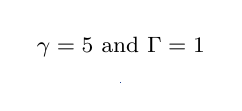
\begin{tikzpicture}[%
font=\footnotesize
]

\begin{axis}[%
width=0.951\figwidth,
height=\figheight,
at={(0\figwidth,0\figheight)},
scale only axis,
xmin=0,
xmax=3,
tick align=outside,
xlabel={Log-Moneyness},
xmajorgrids,
ymin=0,
ymax=5,
ylabel={Remaining Time},
ymajorgrids,
zmin=0,
zmax=250000000,
zlabel={Optimal Rate},
zmajorgrids,
view={50}{40},
axis background/.style={fill=white},
title={$\gamma = 5$ and $\Gamma = 1$},
axis x line*=bottom,
axis y line*=left,
axis z line*=left
]

\addplot3[%
surf,
shader=flat corner,draw=black,z buffer=sort,colormap={mymap}{[1pt] rgb(0pt)=(0.2081,0.1663,0.5292); rgb(1pt)=(0.211624,0.189781,0.577676); rgb(2pt)=(0.212252,0.213771,0.626971); rgb(3pt)=(0.2081,0.2386,0.677086); rgb(4pt)=(0.195905,0.264457,0.7279); rgb(5pt)=(0.170729,0.291938,0.779248); rgb(6pt)=(0.125271,0.324243,0.830271); rgb(7pt)=(0.0591333,0.359833,0.868333); rgb(8pt)=(0.0116952,0.38751,0.881957); rgb(9pt)=(0.00595714,0.408614,0.882843); rgb(10pt)=(0.0165143,0.4266,0.878633); rgb(11pt)=(0.0328524,0.443043,0.871957); rgb(12pt)=(0.0498143,0.458571,0.864057); rgb(13pt)=(0.0629333,0.47369,0.855438); rgb(14pt)=(0.0722667,0.488667,0.8467); rgb(15pt)=(0.0779429,0.503986,0.838371); rgb(16pt)=(0.0793476,0.520024,0.831181); rgb(17pt)=(0.0749429,0.537543,0.826271); rgb(18pt)=(0.0640571,0.556986,0.823957); rgb(19pt)=(0.0487714,0.577224,0.822829); rgb(20pt)=(0.0343429,0.596581,0.819852); rgb(21pt)=(0.0265,0.6137,0.8135); rgb(22pt)=(0.0238905,0.628662,0.803762); rgb(23pt)=(0.0230905,0.641786,0.791267); rgb(24pt)=(0.0227714,0.653486,0.776757); rgb(25pt)=(0.0266619,0.664195,0.760719); rgb(26pt)=(0.0383714,0.674271,0.743552); rgb(27pt)=(0.0589714,0.683757,0.725386); rgb(28pt)=(0.0843,0.692833,0.706167); rgb(29pt)=(0.113295,0.7015,0.685857); rgb(30pt)=(0.145271,0.709757,0.664629); rgb(31pt)=(0.180133,0.717657,0.642433); rgb(32pt)=(0.217829,0.725043,0.619262); rgb(33pt)=(0.258643,0.731714,0.595429); rgb(34pt)=(0.302171,0.737605,0.571186); rgb(35pt)=(0.348167,0.742433,0.547267); rgb(36pt)=(0.395257,0.7459,0.524443); rgb(37pt)=(0.44201,0.748081,0.503314); rgb(38pt)=(0.487124,0.749062,0.483976); rgb(39pt)=(0.530029,0.749114,0.466114); rgb(40pt)=(0.570857,0.748519,0.44939); rgb(41pt)=(0.609852,0.747314,0.433686); rgb(42pt)=(0.6473,0.7456,0.4188); rgb(43pt)=(0.683419,0.743476,0.404433); rgb(44pt)=(0.71841,0.741133,0.390476); rgb(45pt)=(0.752486,0.7384,0.376814); rgb(46pt)=(0.785843,0.735567,0.363271); rgb(47pt)=(0.818505,0.732733,0.34979); rgb(48pt)=(0.850657,0.7299,0.336029); rgb(49pt)=(0.882433,0.727433,0.3217); rgb(50pt)=(0.913933,0.725786,0.306276); rgb(51pt)=(0.944957,0.726114,0.288643); rgb(52pt)=(0.973895,0.731395,0.266648); rgb(53pt)=(0.993771,0.745457,0.240348); rgb(54pt)=(0.999043,0.765314,0.216414); rgb(55pt)=(0.995533,0.786057,0.196652); rgb(56pt)=(0.988,0.8066,0.179367); rgb(57pt)=(0.978857,0.827143,0.163314); rgb(58pt)=(0.9697,0.848138,0.147452); rgb(59pt)=(0.962586,0.870514,0.1309); rgb(60pt)=(0.958871,0.8949,0.113243); rgb(61pt)=(0.959824,0.921833,0.0948381); rgb(62pt)=(0.9661,0.951443,0.0755333); rgb(63pt)=(0.9763,0.9831,0.0538)},mesh/rows=25]
table[row sep=crcr, point meta=\thisrow{c}] {%
%
x	y	z	c\\
0	0.01	32.6488389864948	32.6488389864948\\
0	0.111836734693878	41.368964346008	41.368964346008\\
0	0.213673469387755	55.020392221554	55.020392221554\\
0	0.315510204081633	75.1957385769636	75.1957385769636\\
0	0.41734693877551	103.958848673592	103.958848673592\\
0	0.519183673469388	144.276011427311	144.276011427311\\
0	0.621020408163265	200.330781886104	200.330781886104\\
0	0.722857142857143	277.959747832576	277.959747832576\\
0	0.82469387755102	385.261306025867	385.261306025867\\
0	0.926530612244898	533.441537072205	533.441537072205\\
0	1.02836734693878	737.985546956987	737.985546956987\\
0	1.13020408163265	1020.27668174796	1020.27668174796\\
0	1.23204081632653	1409.83291062371	1409.83291062371\\
0	1.33387755102041	1947.39426220375	1947.39426220375\\
0	1.43571428571429	2689.18424436036	2689.18424436036\\
0	1.53755102040816	3712.79099631399	3712.79099631399\\
0	1.63938775510204	5125.28336417861	5125.28336417861\\
0	1.74122448979592	7074.41088379386	7074.41088379386\\
0	1.8430612244898	9764.05925492452	9764.05925492452\\
0	1.94489795918367	13475.5780454751	13475.5780454751\\
0	2.04673469387755	18597.2116397571	18597.2116397571\\
0	2.14857142857143	25664.7120984615	25664.7120984615\\
0	2.25040816326531	35417.3823002706	35417.3823002706\\
0	2.35224489795918	48875.4118444193	48875.4118444193\\
0	2.45408163265306	67446.595556805	67446.595556805\\
0	2.55591836734694	93073.5980559655	93073.5980559655\\
0	2.65775510204082	128437.16921981	128437.16921981\\
0	2.75959183673469	177236.568226653	177236.568226653\\
0	2.86142857142857	244576.53036801	244576.53036801\\
0	2.96326530612245	337501.255906143	337501.255906143\\
0	3.06510204081633	465731.279720642	465731.279720642\\
0	3.1669387755102	642680.303153884	642680.303153884\\
0	3.26877551020408	886858.355352261	886858.355352261\\
0	3.37061224489796	1223808.06400308	1223808.06400308\\
0	3.47244897959184	1688776.58211775	1688776.58211775\\
0	3.57428571428571	2330402.67197023	2330402.67197023\\
0	3.67612244897959	3215804.63941195	3215804.63941195\\
0	3.77795918367347	4437601.34994115	4437601.34994115\\
0	3.87979591836735	6123600.77097679	6123600.77097679\\
0	3.98163265306122	8450169.52554678	8450169.52554678\\
0	4.0834693877551	11660682.0006254	11660682.0006254\\
0	4.18530612244898	16090978.9081204	16090978.9081204\\
0	4.28714285714286	22204498.4314176	22204498.4314176\\
0	4.38897959183674	30640754.9063498	30640754.9063498\\
0	4.49081632653061	42282236.2253352	42282236.2253352\\
0	4.59265306122449	58346717.8731122	58346717.8731122\\
0	4.69448979591837	80514650.2489909	80514650.2489909\\
0	4.79632653061224	111104944.827116	111104944.827116\\
0	4.89816326530612	153317547.543032	153317547.543032\\
0	5	211568174.177263	211568174.177263\\
0.125	0.01	31.9583503874349	31.9583503874349\\
0.125	0.111836734693878	38.422801117001	38.422801117001\\
0.125	0.213673469387755	49.802474205826	49.802474205826\\
0.125	0.315510204081633	67.0979480337772	67.0979480337772\\
0.125	0.41734693877551	92.0727512791044	92.0727512791044\\
0.125	0.519183673469388	127.3055828865	127.3055828865\\
0.125	0.621020408163265	176.455328942532	176.455328942532\\
0.125	0.722857142857143	244.641756366423	244.641756366423\\
0.125	0.82469387755102	338.979744172372	338.979744172372\\
0.125	0.926530612244898	469.322637208833	469.322637208833\\
0.125	1.02836734693878	649.292332116368	649.292332116368\\
0.125	1.13020408163265	897.703757390111	897.703757390111\\
0.125	1.23204081632653	1240.53269964392	1240.53269964392\\
0.125	1.33387755102041	1713.63278646291	1713.63278646291\\
0.125	1.43571428571429	2366.48581570215	2366.48581570215\\
0.125	1.53755102040816	3267.37772393704	3267.37772393704\\
0.125	1.63938775510204	4510.54162314384	4510.54162314384\\
0.125	1.74122448979592	6226.01510633657	6226.01510633657\\
0.125	1.8430612244898	8593.24295541875	8593.24295541875\\
0.125	1.94489795918367	11859.8481812123	11859.8481812123\\
0.125	2.04673469387755	16367.5349624754	16367.5349624754\\
0.125	2.14857142857143	22587.8331055051	22587.8331055051\\
0.125	2.25040816326531	31171.4231235112	31171.4231235112\\
0.125	2.35224489795918	43016.2016637839	43016.2016637839\\
0.125	2.45408163265306	59361.2073725342	59361.2073725342\\
0.125	2.55591836734694	81916.2324642645	81916.2324642645\\
0.125	2.65775510204082	113040.678214887	113040.678214887\\
0.125	2.75959183673469	155990.363720747	155990.363720747\\
0.125	2.86142857142857	215258.106235195	215258.106235195\\
0.125	2.96326530612245	297043.699085251	297043.699085251\\
0.125	3.06510204081633	409902.450955539	409902.450955539\\
0.125	3.1669387755102	565640.127383986	565640.127383986\\
0.125	3.26877551020408	780547.911447273	780547.911447273\\
0.125	3.37061224489796	1077106.56861236	1077106.56861236\\
0.125	3.47244897959184	1486338.08260192	1486338.08260192\\
0.125	3.57428571428571	2051050.75884644	2051050.75884644\\
0.125	3.67612244897959	2830317.2546798	2830317.2546798\\
0.125	3.77795918367347	3905653.96767853	3905653.96767853\\
0.125	3.87979591836735	5389548.18679295	5389548.18679295\\
0.125	3.98163265306122	7437225.00234227	7437225.00234227\\
0.125	4.0834693877551	10262884.8710236	10262884.8710236\\
0.125	4.18530612244898	14162110.3919926	14162110.3919926\\
0.125	4.28714285714286	19542786.1901136	19542786.1901136\\
0.125	4.38897959183674	26967766.3294558	26967766.3294558\\
0.125	4.49081632653061	37213752.5490174	37213752.5490174\\
0.125	4.59265306122449	51352542.3712437	51352542.3712437\\
0.125	4.69448979591837	70863146.1696756	70863146.1696756\\
0.125	4.79632653061224	97786501.3781487	97786501.3781487\\
0.125	4.89816326530612	134938967.965036	134938967.965036\\
0.125	5	186206938.202814	186206938.202814\\
0.25	0.01	31.9548698781664	31.9548698781664\\
0.25	0.111836734693878	37.48054152924	37.48054152924\\
0.25	0.213673469387755	47.5629761588587	47.5629761588587\\
0.25	0.315510204081633	63.1866582986741	63.1866582986741\\
0.25	0.41734693877551	85.962166722647	85.962166722647\\
0.25	0.519183673469388	118.258738405528	118.258738405528\\
0.25	0.621020408163265	163.443759894189	163.443759894189\\
0.25	0.722857142857143	226.233969679849	226.233969679849\\
0.25	0.82469387755102	313.188682870053	313.188682870053\\
0.25	0.926530612244898	433.395854962318	433.395854962318\\
0.25	1.02836734693878	599.422658437993	599.422658437993\\
0.25	1.13020408163265	828.630006413778	828.630006413778\\
0.25	1.23204081632653	1144.98853698374	1144.98853698374\\
0.25	1.33387755102041	1581.58602561404	1581.58602561404\\
0.25	1.43571428571429	2184.08851854457	2184.08851854457\\
0.25	1.53755102040816	3015.51724434698	3015.51724434698\\
0.25	1.63938775510204	4162.84099927103	4162.84099927103\\
0.25	1.74122448979592	5746.07361181283	5746.07361181283\\
0.25	1.8430612244898	7930.82814370179	7930.82814370179\\
0.25	1.94489795918367	10945.6410700683	10945.6410700683\\
0.25	2.04673469387755	15105.8786713565	15105.8786713565\\
0.25	2.14857142857143	20846.7263952667	20846.7263952667\\
0.25	2.25040816326531	28768.7120947993	28768.7120947993\\
0.25	2.35224489795918	39700.5251715856	39700.5251715856\\
0.25	2.45408163265306	54785.7029195348	54785.7029195348\\
0.25	2.55591836734694	75602.2520299686	75602.2520299686\\
0.25	2.65775510204082	104327.7185062	104327.7185062\\
0.25	2.75959183673469	143966.973014053	143966.973014053\\
0.25	2.86142857142857	198666.540639294	198666.540639294\\
0.25	2.96326530612245	274148.354125522	274148.354125522\\
0.25	3.06510204081633	378308.30591844	378308.30591844\\
0.25	3.1669387755102	522042.210369704	522042.210369704\\
0.25	3.26877551020408	720385.57754889	720385.57754889\\
0.25	3.37061224489796	994086.426445647	994086.426445647\\
0.25	3.47244897959184	1371775.66416375	1371775.66416375\\
0.25	3.57428571428571	1892962.06704037	1892962.06704037\\
0.25	3.67612244897959	2612165.15840686	2612165.15840686\\
0.25	3.77795918367347	3604618.30917726	3604618.30917726\\
0.25	3.87979591836735	4974138.64308264	4974138.64308264\\
0.25	3.98163265306122	6863986.99038125	6863986.99038125\\
0.25	4.0834693877551	9471853.91260402	9471853.91260402\\
0.25	4.18530612244898	13070539.4350531	13070539.4350531\\
0.25	4.28714285714286	18036489.7230373	18036489.7230373\\
0.25	4.38897959183674	24889175.8257997	24889175.8257997\\
0.25	4.49081632653061	34345433.7636585	34345433.7636585\\
0.25	4.59265306122449	47394450.2887499	47394450.2887499\\
0.25	4.69448979591837	65401238.3229594	65401238.3229594\\
0.25	4.79632653061224	90249426.2841769	90249426.2841769\\
0.25	4.89816326530612	124538298.003211	124538298.003211\\
0.25	5	171854694.902158	171854694.902158\\
0.375	0.01	31.9548697809241	31.9548697809241\\
0.375	0.111836734693878	37.267094797369	37.267094797369\\
0.375	0.213673469387755	46.7361211005524	46.7361211005524\\
0.375	0.315510204081633	61.4560854521991	61.4560854521991\\
0.375	0.41734693877551	82.9933167109473	82.9933167109473\\
0.375	0.519183673469388	113.615106586193	113.615106586193\\
0.375	0.621020408163265	156.533064575153	156.533064575153\\
0.375	0.722857142857143	216.241350061576	216.241350061576\\
0.375	0.82469387755102	298.988176750912	298.988176750912\\
0.375	0.926530612244898	413.430281330272	413.430281330272\\
0.375	1.02836734693878	571.539015676337	571.539015676337\\
0.375	1.13020408163265	789.852970706044	789.852970706044\\
0.375	1.23204081632653	1091.20824075907	1091.20824075907\\
0.375	1.33387755102041	1507.12737151115	1507.12737151115\\
0.375	1.43571428571429	2081.11691900602	2081.11691900602\\
0.375	1.53755102040816	2873.21858338907	2873.21858338907\\
0.375	1.63938775510204	3966.29000667225	3966.29000667225\\
0.375	1.74122448979592	5474.67225418873	5474.67225418873\\
0.375	1.8430612244898	7556.15065978385	7556.15065978385\\
0.375	1.94489795918367	10428.4602207626	10428.4602207626\\
0.375	2.04673469387755	14392.0621174171	14392.0621174171\\
0.375	2.14857142857143	19861.5739321794	19861.5739321794\\
0.375	2.25040816326531	27409.1413769007	27409.1413769007\\
0.375	2.35224489795918	37824.2884967379	37824.2884967379\\
0.375	2.45408163265306	52196.507075934	52196.507075934\\
0.375	2.55591836734694	72029.2246413067	72029.2246413067\\
0.375	2.65775510204082	99397.0728633871	99397.0728633871\\
0.375	2.75959183673469	137162.907669039	137162.907669039\\
0.375	2.86142857142857	189277.282791592	189277.282791592\\
0.375	2.96326530612245	261191.70366344	261191.70366344\\
0.375	3.06510204081633	360428.890724625	360428.890724625\\
0.375	3.1669387755102	497369.705438944	497369.705438944\\
0.375	3.26877551020408	686339.056652759	686339.056652759\\
0.375	3.37061224489796	947104.380241183	947104.380241183\\
0.375	3.47244897959184	1306943.44297864	1306943.44297864\\
0.375	3.57428571428571	1803497.77591845	1803497.77591845\\
0.375	3.67612244897959	2488710.22610882	2488710.22610882\\
0.375	3.77795918367347	3434258.52092862	3434258.52092862\\
0.375	3.87979591836735	4739053.22801524	4739053.22801524\\
0.375	3.98163265306122	6539584.45192483	6539584.45192483\\
0.375	4.0834693877551	9024199.59624286	9024199.59624286\\
0.375	4.18530612244898	12452805.7403351	12452805.7403351\\
0.375	4.28714285714286	17184057.6286729	17184057.6286729\\
0.375	4.38897959183674	23712875.315169	23712875.315169\\
0.375	4.49081632653061	32722216.054792	32722216.054792\\
0.375	4.59265306122449	45154516.1227098	45154516.1227098\\
0.375	4.69448979591837	62310275.8449546	62310275.8449546\\
0.375	4.79632653061224	85984100.4829907	85984100.4829907\\
0.375	4.89816326530612	118652427.743148	118652427.743148\\
0.375	5	163732579.442662	163732579.442662\\
0.5	0.01	31.954869780924	31.954869780924\\
0.5	0.111836734693878	37.235076439036	37.235076439036\\
0.5	0.213673469387755	46.481809870143	46.481809870143\\
0.5	0.315510204081633	60.7684547376947	60.7684547376947\\
0.5	0.41734693877551	81.6493877778258	81.6493877778258\\
0.5	0.519183673469388	111.345036135851	111.345036135851\\
0.5	0.621020408163265	152.986340133142	152.986340133142\\
0.5	0.722857142857143	210.946798176882	210.946798176882\\
0.5	0.82469387755102	291.30230657293	291.30230657293\\
0.5	0.926530612244898	402.468168957977	402.468168957977\\
0.5	1.02836734693878	556.080327460305	556.080327460305\\
0.5	1.13020408163265	768.213192135928	768.213192135928\\
0.5	1.23204081632653	1061.06156984855	1061.06156984855\\
0.5	1.33387755102041	1465.26269884362	1465.26269884362\\
0.5	1.43571428571429	2023.10133036601	2023.10133036601\\
0.5	1.53755102040816	2792.93315669812	2792.93315669812\\
0.5	1.63938775510204	3855.2893230316	3855.2893230316\\
0.5	1.74122448979592	5321.30060726335	5321.30060726335\\
0.5	1.8430612244898	7344.32250058293	7344.32250058293\\
0.5	1.94489795918367	10135.977254504	10135.977254504\\
0.5	2.04673469387755	13988.2910020475	13988.2910020475\\
0.5	2.14857142857143	19304.2416444625	19304.2416444625\\
0.5	2.25040816326531	26639.9130154454	26639.9130154454\\
0.5	2.35224489795918	36762.6649271863	36762.6649271863\\
0.5	2.45408163265306	50731.4040687038	50731.4040687038\\
0.5	2.55591836734694	70007.3526210982	70007.3526210982\\
0.5	2.65775510204082	96606.9017158386	96606.9017158386\\
0.5	2.75959183673469	133312.539213324	133312.539213324\\
0.5	2.86142857142857	183963.91623456	183963.91623456\\
0.5	2.96326530612245	253859.499919179	253859.499919179\\
0.5	3.06510204081633	350310.827929311	350310.827929311\\
0.5	3.1669387755102	483407.343364683	483407.343364683\\
0.5	3.26877551020408	667071.816849859	667071.816849859\\
0.5	3.37061224489796	920516.759883136	920516.759883136\\
0.5	3.47244897959184	1270254.17985909	1270254.17985909\\
0.5	3.57428571428571	1752868.9103538	1752868.9103538\\
0.5	3.67612244897959	2418845.62525456	2418845.62525456\\
0.5	3.77795918367347	3337849.86757363	3337849.86757363\\
0.5	3.87979591836735	4606015.52328156	4606015.52328156\\
0.5	3.98163265306122	6356001.05783607	6356001.05783607\\
0.5	4.0834693877551	8770866.46386475	8770866.46386475\\
0.5	4.18530612244898	12103222.5399667	12103222.5399667\\
0.5	4.28714285714286	16701655.6410957	16701655.6410957\\
0.5	4.38897959183674	23047192.1032675	23047192.1032675\\
0.5	4.49081632653061	31803616.7607116	31803616.7607116\\
0.5	4.59265306122449	43886909.2039176	43886909.2039176\\
0.5	4.69448979591837	60561061.2670955	60561061.2670955\\
0.5	4.79632653061224	83570298.8844667	83570298.8844667\\
0.5	4.89816326530612	115321539.590836	115321539.590836\\
0.5	5	159136171.920616	159136171.920616\\
0.625	0.01	31.954869780924	31.954869780924\\
0.625	0.111836734693878	37.232034926865	37.232034926865\\
0.625	0.213673469387755	46.4183432127714	46.4183432127714\\
0.625	0.315510204081633	60.5273509538913	60.5273509538913\\
0.625	0.41734693877551	81.0899356122053	81.0899356122053\\
0.625	0.519183673469388	110.299090715349	110.299090715349\\
0.625	0.621020408163265	151.242364549288	151.242364549288\\
0.625	0.722857142857143	208.227738896225	208.227738896225\\
0.625	0.82469387755102	287.236148718762	287.236148718762\\
0.625	0.926530612244898	396.548405932399	396.548405932399\\
0.625	1.02836734693878	547.612338200068	547.612338200068\\
0.625	1.13020408163265	756.240973223731	756.240973223731\\
0.625	1.23204081632653	1044.26718051817	1044.26718051817\\
0.625	1.33387755102041	1441.8279059199	1441.8279059199\\
0.625	1.43571428571429	1990.51697833513	1990.51697833513\\
0.625	1.53755102040816	2747.73631658265	2747.73631658265\\
0.625	1.63938775510204	3792.70071792251	3792.70071792251\\
0.625	1.74122448979592	5234.72438068191	5234.72438068191\\
0.625	1.8430612244898	7224.65599449367	7224.65599449367\\
0.625	1.94489795918367	9970.65859021355	9970.65859021355\\
0.625	2.04673469387755	13759.9848303519	13759.9848303519\\
0.625	2.14857142857143	18989.0255821551	18989.0255821551\\
0.625	2.25040816326531	26204.7750543607	26204.7750543607\\
0.625	2.35224489795918	36162.0500256303	36162.0500256303\\
0.625	2.45408163265306	49902.4486737575	49902.4486737575\\
0.625	2.55591836734694	68863.3086195648	68863.3086195648\\
0.625	2.65775510204082	95028.0619142267	95028.0619142267\\
0.625	2.75959183673469	131133.715091012	131133.715091012\\
0.625	2.86142857142857	180957.158059593	180957.158059593\\
0.625	2.96326530612245	249710.251636175	249710.251636175\\
0.625	3.06510204081633	344585.022463084	344585.022463084\\
0.625	3.1669387755102	475505.996291241	475505.996291241\\
0.625	3.26877551020408	656168.368633559	656168.368633559\\
0.625	3.37061224489796	905470.612265489	905470.612265489\\
0.625	3.47244897959184	1249491.38173652	1249491.38173652\\
0.625	3.57428571428571	1724217.51210234	1724217.51210234\\
0.625	3.67612244897959	2379308.47848105	2379308.47848105\\
0.625	3.77795918367347	3283291.10365345	3283291.10365345\\
0.625	3.87979591836735	4530727.91427658	4530727.91427658\\
0.625	3.98163265306122	6252109.00290034	6252109.00290034\\
0.625	4.0834693877551	8627502.14959108	8627502.14959108\\
0.625	4.18530612244898	11905389.0956299	11905389.0956299\\
0.625	4.28714285714286	16428658.3673587	16428658.3673587\\
0.625	4.38897959183674	22670473.6704444	22670473.6704444\\
0.625	4.49081632653061	31283769.9244272	31283769.9244272\\
0.625	4.59265306122449	43169554.548192	43169554.548192\\
0.625	4.69448979591837	59571158.7598848	59571158.7598848\\
0.625	4.79632653061224	82204298.1969271	82204298.1969271\\
0.625	4.89816326530612	113436548.052099	113436548.052099\\
0.625	5	156535007.004924	156535007.004924\\
0.75	0.01	31.954869780924	31.954869780924\\
0.75	0.111836734693878	37.2318571224173	37.2318571224173\\
0.75	0.213673469387755	46.4057468194769	46.4057468194769\\
0.75	0.315510204081633	60.4538375602652	60.4538375602652\\
0.75	0.41734693877551	80.8782127673902	80.8782127673902\\
0.75	0.519183673469388	109.849158157429	109.849158157429\\
0.75	0.621020408163265	150.427364837097	150.427364837097\\
0.75	0.722857142857143	206.883568092052	206.883568092052\\
0.75	0.82469387755102	285.145683210871	285.145683210871\\
0.75	0.926530612244898	393.419442879638	393.419442879638\\
0.75	1.02836734693878	543.047284990024	543.047284990024\\
0.75	1.13020408163265	749.69529415185	749.69529415185\\
0.75	1.23204081632653	1034.99235342261	1034.99235342261\\
0.75	1.33387755102041	1428.79297860834	1428.79297860834\\
0.75	1.43571428571429	1972.30055203709	1972.30055203709\\
0.75	1.53755102040816	2722.37767621522	2722.37767621522\\
0.75	1.63938775510204	3757.49454724595	3757.49454724595\\
0.75	1.74122448979592	5185.93759415862	5185.93759415862\\
0.75	1.8430612244898	7157.13706765604	7157.13706765604\\
0.75	1.94489795918367	9877.29852325988	9877.29852325988\\
0.75	2.04673469387755	13630.9733585389	13630.9733585389\\
0.75	2.14857142857143	18810.8248274465	18810.8248274465\\
0.75	2.25040816326531	25958.7032549739	25958.7032549739\\
0.75	2.35224489795918	35822.3271915545	35822.3271915545\\
0.75	2.45408163265306	49433.4997301745	49433.4997301745\\
0.75	2.55591836734694	68216.0419284563	68216.0419284563\\
0.75	2.65775510204082	94134.7338823024	94134.7338823024\\
0.75	2.75959183673469	129900.843667473	129900.843667473\\
0.75	2.86142857142857	179255.743828348	179255.743828348\\
0.75	2.96326530612245	247362.283563861	247362.283563861\\
0.75	3.06510204081633	341344.856714868	341344.856714868\\
0.75	3.1669387755102	471034.660215624	471034.660215624\\
0.75	3.26877551020408	649998.101943586	649998.101943586\\
0.75	3.37061224489796	896955.936190412	896955.936190412\\
0.75	3.47244897959184	1237741.5776551	1237741.5776551\\
0.75	3.57428571428571	1708003.44647859	1708003.44647859\\
0.75	3.67612244897959	2356934.02737778	2356934.02737778\\
0.75	3.77795918367347	3252415.72698222	3252415.72698222\\
0.75	3.87979591836735	4488121.81988369	4488121.81988369\\
0.75	3.98163265306122	6193315.28904252	6193315.28904252\\
0.75	4.0834693877551	8546370.58368213	8546370.58368213\\
0.75	4.18530612244898	11793432.7594499	11793432.7594499\\
0.75	4.28714285714286	16274165.8695845	16274165.8695845\\
0.75	4.38897959183674	22457284.0580949	22457284.0580949\\
0.75	4.49081632653061	30989582.1409055	30989582.1409055\\
0.75	4.59265306122449	42763594.5961209	42763594.5961209\\
0.75	4.69448979591837	59010960.5386293	59010960.5386293\\
0.75	4.79632653061224	81431261.2692431	81431261.2692431\\
0.75	4.89816326530612	112369807.653092	112369807.653092\\
0.75	5	155062975.055951	155062975.055951\\
0.875	0.01	31.954869780924	31.954869780924\\
0.875	0.111836734693878	37.2318508433486	37.2318508433486\\
0.875	0.213673469387755	46.4037877664574	46.4037877664574\\
0.875	0.315510204081633	60.4345750395432	60.4345750395432\\
0.875	0.41734693877551	80.8060723648631	80.8060723648631\\
0.875	0.519183673469388	109.66995311947	109.66995311947\\
0.875	0.621020408163265	150.068021608097	150.068021608097\\
0.875	0.722857142857143	206.248052259285	206.248052259285\\
0.875	0.82469387755102	284.107218683956	284.107218683956\\
0.875	0.926530612244898	391.808690062861	391.808690062861\\
0.875	1.02836734693878	540.635539756324	540.635539756324\\
0.875	1.13020408163265	746.171134850014	746.171134850014\\
0.875	1.23204081632653	1029.92941054178	1029.92941054178\\
0.875	1.33387755102041	1421.60553190276	1421.60553190276\\
0.875	1.43571428571429	1962.18236052532	1962.18236052532\\
0.875	1.53755102040816	2708.21767568049	2708.21767568049\\
0.875	1.63938775510204	3737.76061902082	3737.76061902082\\
0.875	1.74122448979592	5158.51626171589	5158.51626171589\\
0.875	1.8430612244898	7119.1123624018	7119.1123624018\\
0.875	1.94489795918367	9824.64689433158	9824.64689433158\\
0.875	2.04673469387755	13558.142716829	13558.142716829\\
0.875	2.14857142857143	18710.1536922255	18710.1536922255\\
0.875	2.25040816326531	25819.6192441229	25819.6192441229\\
0.875	2.35224489795918	35630.2410135858	35630.2410135858\\
0.875	2.45408163265306	49168.2789832099	49168.2789832099\\
0.875	2.55591836734694	67849.9050560347	67849.9050560347\\
0.875	2.65775510204082	93629.3439802442	93629.3439802442\\
0.875	2.75959183673469	129203.298135028	129203.298135028\\
0.875	2.86142857142857	178293.040354799	178293.040354799\\
0.875	2.96326530612245	246033.683556345	246033.683556345\\
0.875	3.06510204081633	339511.347331677	339511.347331677\\
0.875	3.1669387755102	468504.412664241	468504.412664241\\
0.875	3.26877551020408	646506.404885711	646506.404885711\\
0.875	3.37061224489796	892137.50515604	892137.50515604\\
0.875	3.47244897959184	1231092.34384817	1231092.34384817\\
0.875	3.57428571428571	1698827.82783188	1698827.82783188\\
0.875	3.67612244897959	2344272.16606261	2344272.16606261\\
0.875	3.77795918367347	3234943.08193788	3234943.08193788\\
0.875	3.87979591836735	4464010.61108495	4464010.61108495\\
0.875	3.98163265306122	6160043.29966448	6160043.29966448\\
0.875	4.0834693877551	8500457.31961166	8500457.31961166\\
0.875	4.18530612244898	11730075.3666937	11730075.3666937\\
0.875	4.28714285714286	16186736.7241411	16186736.7241411\\
0.875	4.38897959183674	22336637.4728874	22336637.4728874\\
0.875	4.49081632653061	30823097.6667623	30823097.6667623\\
0.875	4.59265306122449	42533856.8397966	42533856.8397966\\
0.875	4.69448979591837	58693937.3981512	58693937.3981512\\
0.875	4.79632653061224	80993790.0180224	80993790.0180224\\
0.875	4.89816326530612	111766125.900669	111766125.900669\\
0.875	5	154229933.701062	154229933.701062\\
1	0.01	31.954869780924	31.954869780924\\
1	0.111836734693878	37.2318507110628	37.2318507110628\\
1	0.213673469387755	46.4035515614791	46.4035515614791\\
1	0.315510204081633	60.4302775558077	60.4302775558077\\
1	0.41734693877551	80.7841180090462	80.7841180090462\\
1	0.519183673469388	109.604331477129	109.604331477129\\
1	0.621020408163265	149.919489923836	149.919489923836\\
1	0.722857142857143	205.962362519072	205.962362519072\\
1	0.82469387755102	283.611412145788	283.611412145788\\
1	0.926530612244898	391.004982763524	391.004982763524\\
1	1.02836734693878	539.392225714207	539.392225714207\\
1	1.13020408163265	744.309640170295	744.309640170295\\
1	1.23204081632653	1027.20621771477	1027.20621771477\\
1	1.33387755102041	1417.6871413467	1417.6871413467\\
1	1.43571428571429	1956.61071412487	1956.61071412487\\
1	1.53755102040816	2700.36245819976	2700.36245819976\\
1	1.63938775510204	3726.75347211424	3726.75347211424\\
1	1.74122448979592	5143.16004685306	5143.16004685306\\
1	1.8430612244898	7097.75599428311	7097.75599428311\\
1	1.94489795918367	9795.01266136439	9795.01266136439\\
1	2.04673469387755	13517.0880325276	13517.0880325276\\
1	2.14857142857143	18653.3423605707	18653.3423605707\\
1	2.25040816326531	25741.0678551	25741.0678551\\
1	2.35224489795918	35521.6930218938	35521.6930218938\\
1	2.45408163265306	49018.3409968996	49018.3409968996\\
1	2.55591836734694	67642.8549868627	67642.8549868627\\
1	2.65775510204082	93343.4863816825	93343.4863816825\\
1	2.75959183673469	128808.694686402	128808.694686402\\
1	2.86142857142857	177748.378085963	177748.378085963\\
1	2.96326530612245	245281.95320912	245281.95320912\\
1	3.06510204081633	338473.879786603	338473.879786603\\
1	3.1669387755102	467072.649603958	467072.649603958\\
1	3.26877551020408	644530.542852433	644530.542852433\\
1	3.37061224489796	889410.825096997	889410.825096997\\
1	3.47244897959184	1227329.58691654	1227329.58691654\\
1	3.57428571428571	1693635.35540987	1693635.35540987\\
1	3.67612244897959	2337106.78254889	2337106.78254889\\
1	3.77795918367347	3225055.21289229	3225055.21289229\\
1	3.87979591836735	4450365.89279077	4450365.89279077\\
1	3.98163265306122	6141214.3778609	6141214.3778609\\
1	4.0834693877551	8474474.53883253	8474474.53883253\\
1	4.18530612244898	11694220.7313357	11694220.7313357\\
1	4.28714285714286	16137259.578234	16137259.578234\\
1	4.38897959183674	22268362.1568017	22268362.1568017\\
1	4.49081632653061	30728882.109166	30728882.109166\\
1	4.59265306122449	42403845.4500193	42403845.4500193\\
1	4.69448979591837	58514530.1065862	58514530.1065862\\
1	4.79632653061224	80746219.6194132	80746219.6194132\\
1	4.89816326530612	111424494.881036	111424494.881036\\
1	5	153758505.187455	153758505.187455\\
1.125	0.01	31.954869780924	31.954869780924\\
1.125	0.111836734693878	37.2318507094147	37.2318507094147\\
1.125	0.213673469387755	46.4035296538757	46.4035296538757\\
1.125	0.315510204081633	60.4294670671885	60.4294670671885\\
1.125	0.41734693877551	80.7781891119079	80.7781891119079\\
1.125	0.519183673469388	109.582369594614	109.582369594614\\
1.125	0.621020408163265	149.862249141098	149.862249141098\\
1.125	0.722857142857143	205.840876431485	205.840876431485\\
1.125	0.82469387755102	283.384995660626	283.384995660626\\
1.125	0.926530612244898	390.618033724423	390.618033724423\\
1.125	1.02836734693878	538.769352956556	538.769352956556\\
1.125	1.13020408163265	743.348571810194	743.348571810194\\
1.125	1.23204081632653	1025.76775121546	1025.76775121546\\
1.125	1.33387755102041	1415.58110151054	1415.58110151054\\
1.125	1.43571428571429	1953.57647087017	1953.57647087017\\
1.125	1.53755102040816	2696.04198588516	2696.04198588516\\
1.125	1.63938775510204	3720.65414943058	3720.65414943058\\
1.125	1.74122448979592	5134.60332024998	5134.60332024998\\
1.125	1.8430612244898	7085.80654647232	7085.80654647232\\
1.125	1.94489795918367	9778.38068485029	9778.38068485029\\
1.125	2.04673469387755	13493.9943928233	13493.9943928233\\
1.125	2.14857142857143	18621.3325502323	18621.3325502323\\
1.125	2.25040816326531	25696.7552816625	25696.7552816625\\
1.125	2.35224489795918	35460.4047796713	35460.4047796713\\
1.125	2.45408163265306	48933.6290710111	48933.6290710111\\
1.125	2.55591836734694	67525.8217605553	67525.8217605553\\
1.125	2.65775510204082	93181.8538924473	93181.8538924473\\
1.125	2.75959183673469	128585.520270433	128585.520270433\\
1.125	2.86142857142857	177440.282060101	177440.282060101\\
1.125	2.96326530612245	244856.673195104	244856.673195104\\
1.125	3.06510204081633	337886.89584461	337886.89584461\\
1.125	3.1669387755102	466262.527142806	466262.527142806\\
1.125	3.26877551020408	643412.506154716	643412.506154716\\
1.125	3.37061224489796	887867.889208004	887867.889208004\\
1.125	3.47244897959184	1225200.32023454	1225200.32023454\\
1.125	3.57428571428571	1690696.99286447	1690696.99286447\\
1.125	3.67612244897959	2333051.92289514	2333051.92289514\\
1.125	3.77795918367347	3219459.66250436	3219459.66250436\\
1.125	3.87979591836735	4442644.29220477	4442644.29220477\\
1.125	3.98163265306122	6130558.96931156	6130558.96931156\\
1.125	4.0834693877551	8459770.66946559	8459770.66946559\\
1.125	4.18530612244898	11673930.2531764	11673930.2531764\\
1.125	4.28714285714286	16109259.9477821	16109259.9477821\\
1.125	4.38897959183674	22229724.4030124	22229724.4030124\\
1.125	4.49081632653061	30675564.4438079	30675564.4438079\\
1.125	4.59265306122449	42330270.4700391	42330270.4700391\\
1.125	4.69448979591837	58413001.3610664	58413001.3610664\\
1.125	4.79632653061224	80606116.510192	80606116.510192\\
1.125	4.89816326530612	111231161.6783	111231161.6783\\
1.125	5	153491717.94403	153491717.94403\\
1.25	0.01	31.954869780924	31.954869780924\\
1.25	0.111836734693878	37.2318507094026	37.2318507094026\\
1.25	0.213673469387755	46.4035280997599	46.4035280997599\\
1.25	0.315510204081633	60.4293385671783	60.4293385671783\\
1.25	0.41734693877551	80.7767756921319	80.7767756921319\\
1.25	0.519183673469388	109.575684715031	109.575684715031\\
1.25	0.621020408163265	149.841777272752	149.841777272752\\
1.25	0.722857142857143	205.79222488112	205.79222488112\\
1.25	0.82469387755102	283.286520021629	283.286520021629\\
1.25	0.926530612244898	390.439003599277	390.439003599277\\
1.25	1.02836734693878	538.467280157099	538.467280157099\\
1.25	1.13020408163265	742.865321284861	742.865321284861\\
1.25	1.23204081632653	1025.02397913247	1025.02397913247\\
1.25	1.33387755102041	1414.46841831068	1414.46841831068\\
1.25	1.43571428571429	1951.94650406158	1951.94650406158\\
1.25	1.53755102040816	2693.69120050885	2693.69120050885\\
1.25	1.63938775510204	3717.30284372869	3717.30284372869\\
1.25	1.74122448979592	5129.86660595453	5129.86660595453\\
1.25	1.8430612244898	7079.15428474555	7079.15428474555\\
1.25	1.94489795918367	9769.0821931332	9769.0821931332\\
1.25	2.04673469387755	13481.0421441021	13481.0421441021\\
1.25	2.14857142857143	18603.3368879646	18603.3368879646\\
1.25	2.25040816326531	25671.7991409443	25671.7991409443\\
1.25	2.35224489795918	35425.8432209782	35425.8432209782\\
1.25	2.45408163265306	48885.8126593183	48885.8126593183\\
1.25	2.55591836734694	67459.7148558901	67459.7148558901\\
1.25	2.65775510204082	93090.5079245649	93090.5079245649\\
1.25	2.75959183673469	128459.346900356	128459.346900356\\
1.25	2.86142857142857	177266.05019783	177266.05019783\\
1.25	2.96326530612245	244616.124956106	244616.124956106\\
1.25	3.06510204081633	337554.836665993	337554.836665993\\
1.25	3.1669387755102	465804.190273579	465804.190273579\\
1.25	3.26877551020408	642779.915829132	642779.915829132\\
1.25	3.37061224489796	886994.842066578	886994.842066578\\
1.25	3.47244897959184	1223995.46001683	1223995.46001683\\
1.25	3.57428571428571	1689034.25394135	1689034.25394135\\
1.25	3.67612244897959	2330757.3429715	2330757.3429715\\
1.25	3.77795918367347	3216293.18501454	3216293.18501454\\
1.25	3.87979591836735	4438274.65481185	4438274.65481185\\
1.25	3.98163265306122	6124529.05168259	6124529.05168259\\
1.25	4.0834693877551	8451449.67547241	8451449.67547241\\
1.25	4.18530612244898	11662447.725466	11662447.725466\\
1.25	4.28714285714286	16093414.7122068	16093414.7122068\\
1.25	4.38897959183674	22207858.9179087	22207858.9179087\\
1.25	4.49081632653061	30645391.4102326	30645391.4102326\\
1.25	4.59265306122449	42288633.5652534	42288633.5652534\\
1.25	4.69448979591837	58355545.066417	58355545.066417\\
1.25	4.79632653061224	80526830.4952157	80526830.4952157\\
1.25	4.89816326530612	111121752.080632	111121752.080632\\
1.25	5	153340739.776865	153340739.776865\\
1.375	0.01	31.954869780924	31.954869780924\\
1.375	0.111836734693878	37.2318507094026	37.2318507094026\\
1.375	0.213673469387755	46.4035280157938	46.4035280157938\\
1.375	0.315510204081633	60.4293215132701	60.4293215132701\\
1.375	0.41734693877551	80.7764794831849	80.7764794831849\\
1.375	0.519183673469388	109.573841506998	109.573841506998\\
1.375	0.621020408163265	149.835008798003	149.835008798003\\
1.375	0.722857142857143	205.773945331042	205.773945331042\\
1.375	0.82469387755102	283.245878511113	283.245878511113\\
1.375	0.926530612244898	390.359690240238	390.359690240238\\
1.375	1.02836734693878	538.325962571185	538.325962571185\\
1.375	1.13020408163265	742.629458711066	742.629458711066\\
1.375	1.23204081632653	1024.64872432854	1024.64872432854\\
1.375	1.33387755102041	1413.89224489019	1413.89224489019\\
1.375	1.43571428571429	1951.08507950067	1951.08507950067\\
1.375	1.53755102040816	2692.42885190531	2692.42885190531\\
1.375	1.63938775510204	3715.48071805297	3715.48071805297\\
1.375	1.74122448979592	5127.26628464506	5127.26628464506\\
1.375	1.8430612244898	7075.47513923171	7075.47513923171\\
1.375	1.94489795918367	9763.91011432752	9763.91011432752\\
1.375	2.04673469387755	13473.8063771261	13473.8063771261\\
1.375	2.14857142857143	18593.2504592847	18593.2504592847\\
1.375	2.25040816326531	25657.7766487193	25657.7766487193\\
1.375	2.35224489795918	35406.3873913092	35406.3873913092\\
1.375	2.45408163265306	48858.8578035944	48858.8578035944\\
1.375	2.55591836734694	67422.4108557655	67422.4108557655\\
1.375	2.65775510204082	93038.9221496793	93038.9221496793\\
1.375	2.75959183673469	128388.05287892	128388.05287892\\
1.375	2.86142857142857	177167.56001361	177167.56001361\\
1.375	2.96326530612245	244480.105997921	244480.105997921\\
1.375	3.06510204081633	337367.030797548	337367.030797548\\
1.375	3.1669387755102	465544.922362508	465544.922362508\\
1.375	3.26877551020408	642422.035618323	642422.035618323\\
1.375	3.37061224489796	886500.884094591	886500.884094591\\
1.375	3.47244897959184	1223313.72449694	1223313.72449694\\
1.375	3.57428571428571	1688093.39863387	1688093.39863387\\
1.375	3.67612244897959	2329458.92032404	2329458.92032404\\
1.375	3.77795918367347	3214501.34390634	3214501.34390634\\
1.375	3.87979591836735	4435801.92963727	4435801.92963727\\
1.375	3.98163265306122	6121116.75221865	6121116.75221865\\
1.375	4.0834693877551	8446740.82618186	8446740.82618186\\
1.375	4.18530612244898	11655949.7235092	11655949.7235092\\
1.375	4.28714285714286	16084447.7979453	16084447.7979453\\
1.375	4.38897959183674	22195485.0675761	22195485.0675761\\
1.375	4.49081632653061	30628316.2124795	30628316.2124795\\
1.375	4.59265306122449	42265070.8172067	42265070.8172067\\
1.375	4.69448979591837	58323029.9251129	58323029.9251129\\
1.375	4.79632653061224	80481961.638816	80481961.638816\\
1.375	4.89816326530612	111059835.907794	111059835.907794\\
1.375	5	153255299.425175	153255299.425175\\
1.5	0.01	31.954869780924	31.954869780924\\
1.5	0.111836734693878	37.2318507094026	37.2318507094026\\
1.5	0.213673469387755	46.4035280123499	46.4035280123499\\
1.5	0.315510204081633	60.4293196249927	60.4293196249927\\
1.5	0.41734693877551	80.7764250950916	80.7764250950916\\
1.5	0.519183673469388	109.573382644132	109.573382644132\\
1.5	0.621020408163265	149.832946732427	149.832946732427\\
1.5	0.722857142857143	205.767522190086	205.767522190086\\
1.5	0.82469387755102	283.230012957733	283.230012957733\\
1.5	0.926530612244898	390.32615151114	390.32615151114\\
1.5	1.02836734693878	538.262385643008	538.262385643008\\
1.5	1.13020408163265	742.518057989058	742.518057989058\\
1.5	1.23204081632653	1024.46452969699	1024.46452969699\\
1.5	1.33387755102041	1413.6006412724	1413.6006412724\\
1.5	1.43571428571429	1950.63836707982	1950.63836707982\\
1.5	1.53755102040816	2691.76144946197	2691.76144946197\\
1.5	1.63938775510204	3714.50249594171	3714.50249594171\\
1.5	1.74122448979592	5125.85332265419	5125.85332265419\\
1.5	1.8430612244898	7073.45693825702	7073.45693825702\\
1.5	1.94489795918367	9761.05192191371	9761.05192191371\\
1.5	2.04673469387755	13469.7847771774	13469.7847771774\\
1.5	2.14857142857143	18587.6196725069	18587.6196725069\\
1.5	2.25040816326531	25649.9220191688	25649.9220191688\\
1.5	2.35224489795918	35395.4611943105	35395.4611943105\\
1.5	2.45408163265306	48843.690661135	48843.690661135\\
1.5	2.55591836734694	67401.3894939136	67401.3894939136\\
1.5	2.65775510204082	93009.8207117118	93009.8207117118\\
1.5	2.75959183673469	128347.800149424	128347.800149424\\
1.5	2.86142857142857	177111.918204622	177111.918204622\\
1.5	2.96326530612245	244403.227496894	244403.227496894\\
1.5	3.06510204081633	337260.846510867	337260.846510867\\
1.5	3.1669387755102	465398.297671982	465398.297671982\\
1.5	3.26877551020408	642219.605658785	642219.605658785\\
1.5	3.37061224489796	886221.446515563	886221.446515563\\
1.5	3.47244897959184	1222928.02158118	1222928.02158118\\
1.5	3.57428571428571	1687561.05676824	1687561.05676824\\
1.5	3.67612244897959	2328724.22667167	2328724.22667167\\
1.5	3.77795918367347	3213487.41849255	3213487.41849255\\
1.5	3.87979591836735	4434402.68321138	4434402.68321138\\
1.5	3.98163265306122	6119185.78863158	6119185.78863158\\
1.5	4.0834693877551	8444076.12839526	8444076.12839526\\
1.5	4.18530612244898	11652272.5212924	11652272.5212924\\
1.5	4.28714285714286	16079373.4066824	16079373.4066824\\
1.5	4.38897959183674	22188482.6477307	22188482.6477307\\
1.5	4.49081632653061	30618653.2402928	30618653.2402928\\
1.5	4.59265306122449	42251736.4578989	42251736.4578989\\
1.5	4.69448979591837	58304629.2929214	58304629.2929214\\
1.5	4.79632653061224	80456569.8827748	80456569.8827748\\
1.5	4.89816326530612	111024796.859668	111024796.859668\\
1.5	5	153206947.746799	153206947.746799\\
1.625	0.01	31.954869780924	31.954869780924\\
1.625	0.111836734693878	37.2318507094026	37.2318507094026\\
1.625	0.213673469387755	46.403528012243	46.403528012243\\
1.625	0.315510204081633	60.429319451013	60.429319451013\\
1.625	0.41734693877551	80.7764163688989	80.7764163688989\\
1.625	0.519183673469388	109.573279783442	109.573279783442\\
1.625	0.621020408163265	149.832369400271	149.832369400271\\
1.625	0.722857142857143	205.765417072823	205.765417072823\\
1.625	0.82469387755102	283.224170261281	283.224170261281\\
1.625	0.926530612244898	390.312651108235	390.312651108235\\
1.625	1.02836734693878	538.23495505133	538.23495505133\\
1.625	1.13020408163265	742.467280105355	742.467280105355\\
1.625	1.23204081632653	1024.37680496711	1024.37680496711\\
1.625	1.33387755102041	1413.45677751555	1413.45677751555\\
1.625	1.43571428571429	1950.41163141789	1950.41163141789\\
1.625	1.53755102040816	2691.41486313566	2691.41486313566\\
1.625	1.63938775510204	3713.9850768084	3713.9850768084\\
1.625	1.74122448979592	5125.09487310827	5125.09487310827\\
1.625	1.8430612244898	7072.36082670184	7072.36082670184\\
1.625	1.94489795918367	9759.48509804479	9759.48509804479\\
1.625	2.04673469387755	13467.5639735121	13467.5639735121\\
1.625	2.14857142857143	18584.4923467912	18584.4923467912\\
1.625	2.25040816326531	25645.5400429773	25645.5400429773\\
1.625	2.35224489795918	35389.3445349432	35389.3445349432\\
1.625	2.45408163265306	48835.1772575516	48835.1772575516\\
1.625	2.55591836734694	67389.5660835227	67389.5660835227\\
1.625	2.65775510204082	92993.4273723416	92993.4273723416\\
1.625	2.75959183673469	128325.098571345	128325.098571345\\
1.625	2.86142857142857	177080.509913473	177080.509913473\\
1.625	2.96326530612245	244359.80301293	244359.80301293\\
1.625	3.06510204081633	337200.839205421	337200.839205421\\
1.625	3.1669387755102	465315.406112742	465315.406112742\\
1.625	3.26877551020408	642105.134478517	642105.134478517\\
1.625	3.37061224489796	886063.396855249	886063.396855249\\
1.625	3.47244897959184	1222709.83596234	1222709.83596234\\
1.625	3.57428571428571	1687259.88710021	1687259.88710021\\
1.625	3.67612244897959	2328308.54421633	2328308.54421633\\
1.625	3.77795918367347	3212913.71577345	3212913.71577345\\
1.625	3.87979591836735	4433610.92286552	4433610.92286552\\
1.625	3.98163265306122	6118093.12312407	6118093.12312407\\
1.625	4.0834693877551	8442568.23363798	8442568.23363798\\
1.625	4.18530612244898	11650191.6376064	11650191.6376064\\
1.625	4.28714285714286	16076501.8361103	16076501.8361103\\
1.625	4.38897959183674	22184519.9814094	22184519.9814094\\
1.625	4.49081632653061	30613184.9337205	30613184.9337205\\
1.625	4.59265306122449	42244190.4668628	42244190.4668628\\
1.625	4.69448979591837	58294216.2339185	58294216.2339185\\
1.625	4.79632653061224	80442200.4583138	80442200.4583138\\
1.625	4.89816326530612	111004967.910594	111004967.910594\\
1.625	5	153179585.01197	153179585.01197\\
1.75	0.01	31.954869780924	31.954869780924\\
1.75	0.111836734693878	37.2318507094026	37.2318507094026\\
1.75	0.213673469387755	46.4035280122404	46.4035280122404\\
1.75	0.315510204081633	60.4293194377015	60.4293194377015\\
1.75	0.41734693877551	80.7764151481559	80.7764151481559\\
1.75	0.519183673469388	109.573259067023	109.573259067023\\
1.75	0.621020408163265	149.832221185881	149.832221185881\\
1.75	0.722857142857143	205.764775018594	205.764775018594\\
1.75	0.82469387755102	283.222145144883	283.222145144883\\
1.75	0.926530612244898	390.307490093126	390.307490093126\\
1.75	1.02836734693878	538.223631735604	538.223631735604\\
1.75	1.13020408163265	742.444997017048	742.444997017048\\
1.75	1.23204081632653	1024.33636483431	1024.33636483431\\
1.75	1.33387755102041	1413.38775568604	1413.38775568604\\
1.75	1.43571428571429	1950.29925590125	1950.29925590125\\
1.75	1.53755102040816	2691.23847638318	2691.23847638318\\
1.75	1.63938775510204	3713.7160096682	3713.7160096682\\
1.75	1.74122448979592	5124.69350085616	5124.69350085616\\
1.75	1.8430612244898	7071.77249275701	7071.77249275701\\
1.75	1.94489795918367	9758.63447381733	9758.63447381733\\
1.75	2.04673469387755	13466.3472604009	13466.3472604009\\
1.75	2.14857142857143	18582.7665016119	18582.7665016119\\
1.75	2.25040816326531	25643.107897536	25643.107897536\\
1.75	2.35224489795918	35385.9342516109	35385.9342516109\\
1.75	2.45408163265306	48830.413970698	48830.413970698\\
1.75	2.55591836734694	67382.9327596354	67382.9327596354\\
1.75	2.65775510204082	92984.2107941439	92984.2107941439\\
1.75	2.75959183673469	128312.314795307	128312.314795307\\
1.75	2.86142857142857	177062.801403043	177062.801403043\\
1.75	2.96326530612245	244335.296687017	244335.296687017\\
1.75	3.06510204081633	337166.950553206	337166.950553206\\
1.75	3.1669387755102	465268.568884135	465268.568884135\\
1.75	3.26877551020408	642040.42767432	642040.42767432\\
1.75	3.37061224489796	885974.029997983	885974.029997983\\
1.75	3.47244897959184	1222586.43880392	1222586.43880392\\
1.75	3.57428571428571	1687089.52946549	1687089.52946549\\
1.75	3.67612244897959	2328073.38345186	2328073.38345186\\
1.75	3.77795918367347	3212589.13031605	3212589.13031605\\
1.75	3.87979591836735	4433162.93668977	4433162.93668977\\
1.75	3.98163265306122	6117474.85164925	6117474.85164925\\
1.75	4.0834693877551	8441714.97931316	8441714.97931316\\
1.75	4.18530612244898	11649014.1221398	11649014.1221398\\
1.75	4.28714285714286	16074876.8613895	16074876.8613895\\
1.75	4.38897959183674	22182277.5421843	22182277.5421843\\
1.75	4.49081632653061	30610090.4339499	30610090.4339499\\
1.75	4.59265306122449	42239920.1794381	42239920.1794381\\
1.75	4.69448979591837	58288323.4366912	58288323.4366912\\
1.75	4.79632653061224	80434068.7040314	80434068.7040314\\
1.75	4.89816326530612	110993746.542473	110993746.542473\\
1.75	5	153164100.179413	153164100.179413\\
1.875	0.01	31.954869780924	31.954869780924\\
1.875	0.111836734693878	37.2318507094026	37.2318507094026\\
1.875	0.213673469387755	46.4035280122404	46.4035280122404\\
1.875	0.315510204081633	60.4293194368571	60.4293194368571\\
1.875	0.41734693877551	80.7764149995133	80.7764149995133\\
1.875	0.519183673469388	109.573255325144	109.573255325144\\
1.875	0.621020408163265	149.832186361119	149.832186361119\\
1.875	0.722857142857143	205.764593128391	205.764593128391\\
1.875	0.82469387755102	283.221485784853	283.221485784853\\
1.875	0.926530612244898	390.305620067167	390.305620067167\\
1.875	1.02836734693878	538.219168732691	538.219168732691\\
1.875	1.13020408163265	742.435602376651	742.435602376651\\
1.875	1.23204081632653	1024.31835869886	1024.31835869886\\
1.875	1.33387755102041	1413.35562201133	1413.35562201133\\
1.875	1.43571428571429	1950.24498745795	1950.24498745795\\
1.875	1.53755102040816	2691.1506894931	2691.1506894931\\
1.875	1.63938775510204	3713.57873240323	3713.57873240323\\
1.875	1.74122448979592	5124.48450351308	5124.48450351308\\
1.875	1.8430612244898	7071.46098149568	7071.46098149568\\
1.875	1.94489795918367	9758.17790207601	9758.17790207601\\
1.875	2.04673469387755	13465.6869209379	13465.6869209379\\
1.875	2.14857142857143	18581.8214350413	18581.8214350413\\
1.875	2.25040816326531	25641.7664776742	25641.7664776742\\
1.875	2.35224489795918	35384.0425654297	35384.0425654297\\
1.875	2.45408163265306	48827.7597758089	48827.7597758089\\
1.875	2.55591836734694	67379.2233399722	67379.2233399722\\
1.875	2.65775510204082	92979.0423965228	92979.0423965228\\
1.875	2.75959183673469	128305.130449087	128305.130449087\\
1.875	2.86142857142857	177052.832710099	177052.832710099\\
1.875	2.96326530612245	244321.483492573	244321.483492573\\
1.875	3.06510204081633	337147.830094399	337147.830094399\\
1.875	3.1669387755102	465242.12282042	465242.12282042\\
1.875	3.26877551020408	642003.87099807	642003.87099807\\
1.875	3.37061224489796	885923.519743982	885923.519743982\\
1.875	3.47244897959184	1222516.6720869	1222516.6720869\\
1.875	3.57428571428571	1686993.18879786	1686993.18879786\\
1.875	3.67612244897959	2327940.37131843	2327940.37131843\\
1.875	3.77795918367347	3212405.51293717	3212405.51293717\\
1.875	3.87979591836735	4432909.48648386	4432909.48648386\\
1.875	3.98163265306122	6117125.03592676	6117125.03592676\\
1.875	4.0834693877551	8441232.18480622	8441232.18480622\\
1.875	4.18530612244898	11648347.8250353	11648347.8250353\\
1.875	4.28714285714286	16073957.3422262	16073957.3422262\\
1.875	4.38897959183674	22181008.5927569	22181008.5927569\\
1.875	4.49081632653061	30608339.2933151	30608339.2933151\\
1.875	4.59265306122449	42237503.6462628	42237503.6462628\\
1.875	4.69448979591837	58284988.7052028	58284988.7052028\\
1.875	4.79632653061224	80429466.9188845	80429466.9188845\\
1.875	4.89816326530612	110987396.3062	110987396.3062\\
1.875	5	153155337.195091	153155337.195091\\
2	0.01	31.954869780924	31.954869780924\\
2	0.111836734693878	37.2318507094026	37.2318507094026\\
2	0.213673469387755	46.4035280122404	46.4035280122404\\
2	0.315510204081633	60.4293194368128	60.4293194368128\\
2	0.41734693877551	80.776414983782	80.776414983782\\
2	0.519183673469388	109.57325471991	109.57325471991\\
2	0.621020408163265	149.832178883832	149.832178883832\\
2	0.722857142857143	205.76454534306	205.76454534306\\
2	0.82469387755102	283.221284451086	283.221284451086\\
2	0.926530612244898	390.304978936093	390.304978936093\\
2	1.02836734693878	538.217492119006	538.217492119006\\
2	1.13020408163265	742.431803984049	742.431803984049\\
2	1.23204081632653	1024.3106295385	1024.3106295385\\
2	1.33387755102041	1413.34113295947	1413.34113295947\\
2	1.43571428571429	1950.21950146283	1950.21950146283\\
2	1.53755102040816	2691.10804575009	2691.10804575009\\
2	1.63938775510204	3713.51014903463	3713.51014903463\\
2	1.74122448979592	5124.37762474912	5124.37762474912\\
2	1.8430612244898	7071.29856774265	7071.29856774265\\
2	1.94489795918367	9757.93602349865	9757.93602349865\\
2	2.04673469387755	13465.3324631619	13465.3324631619\\
2	2.14857142857143	18581.3086537335	18581.3086537335\\
2	2.25040816326531	25641.0322394756	25641.0322394756\\
2	2.35224489795918	35382.999775563	35382.999775563\\
2	2.45408163265306	48826.2883032639	48826.2883032639\\
2	2.55591836734694	67377.1574896637	67377.1574896637\\
2	2.65775510204082	92976.1536168417	92976.1536168417\\
2	2.75959183673469	128301.103465066	128301.103465066\\
2	2.86142857142857	177047.232584866	177047.232584866\\
2	2.96326530612245	244313.710170973	244313.710170973\\
2	3.06510204081633	337137.055673311	337137.055673311\\
2	3.1669387755102	465227.204983543	465227.204983543\\
2	3.26877551020408	641983.233559655	641983.233559655\\
2	3.37061224489796	885894.987805435	885894.987805435\\
2	3.47244897959184	1222477.24456246	1222477.24456246\\
2	3.57428571428571	1686938.72451402	1686938.72451402\\
2	3.67612244897959	2327865.1558509	2327865.1558509\\
2	3.77795918367347	3212301.66087385	3212301.66087385\\
2	3.87979591836735	4432766.11658653	4432766.11658653\\
2	3.98163265306122	6116927.13290796	6116927.13290796\\
2	4.0834693877551	8440959.02865591	8440959.02865591\\
2	4.18530612244898	11647970.8235945	11647970.8235945\\
2	4.28714285714286	16073437.0402804	16073437.0402804\\
2	4.38897959183674	22180290.5447815	22180290.5447815\\
2	4.49081632653061	30607348.3681342	30607348.3681342\\
2	4.59265306122449	42236136.1678519	42236136.1678519\\
2	4.69448979591837	58283101.6075106	58283101.6075106\\
2	4.79632653061224	80426862.7801994	80426862.7801994\\
2	4.89816326530612	110983802.697554	110983802.697554\\
2	5	153150378.182414	153150378.182414\\
2.125	0.01	31.954869780924	31.954869780924\\
2.125	0.111836734693878	37.2318507094026	37.2318507094026\\
2.125	0.213673469387755	46.4035280122404	46.4035280122404\\
2.125	0.315510204081633	60.4293194368108	60.4293194368108\\
2.125	0.41734693877551	80.7764149823367	80.7764149823367\\
2.125	0.519183673469388	109.573254632357	109.573254632357\\
2.125	0.621020408163265	149.832177418646	149.832177418646\\
2.125	0.722857142857143	205.764533716772	205.764533716772\\
2.125	0.82469387755102	283.221226877283	283.221226877283\\
2.125	0.926530612244898	390.304771252064	390.304771252064\\
2.125	1.02836734693878	538.216892691888	538.216892691888\\
2.125	1.13020408163265	742.430333525693	742.430333525693\\
2.125	1.23204081632653	1024.30743624254	1024.30743624254\\
2.125	1.33387755102041	1413.33481624201	1413.33481624201\\
2.125	1.43571428571429	1950.20788215119	1950.20788215119\\
2.125	1.53755102040816	2691.08786321622	2691.08786321622\\
2.125	1.63938775510204	3713.47665636463	3713.47665636463\\
2.125	1.74122448979592	5124.32404089223	5124.32404089223\\
2.125	1.8430612244898	7071.21532951238	7071.21532951238\\
2.125	1.94489795918367	9757.80975860574	9757.80975860574\\
2.125	2.04673469387755	13465.1445758126	13465.1445758126\\
2.125	2.14857142857143	18581.0333735545	18581.0333735545\\
2.125	2.25040816326531	25640.633928301	25640.633928301\\
2.125	2.35224489795918	35382.4292089997	35382.4292089997\\
2.125	2.45408163265306	48825.4775367907	48825.4775367907\\
2.125	2.55591836734694	67376.0127710634	67376.0127710634\\
2.125	2.65775510204082	92974.5456025351	92974.5456025351\\
2.125	2.75959183673469	128298.853716018	128298.853716018\\
2.125	2.86142857142857	177044.094928687	177044.094928687\\
2.125	2.96326530612245	244309.344979919	244309.344979919\\
2.125	3.06510204081633	337130.99436697	337130.99436697\\
2.125	3.1669387755102	465218.801042507	465218.801042507\\
2.125	3.26877551020408	641971.594925529	641971.594925529\\
2.125	3.37061224489796	885878.883595509	885878.883595509\\
2.125	3.47244897959184	1222454.97634055	1222454.97634055\\
2.125	3.57428571428571	1686907.94865137	1686907.94865137\\
2.125	3.67612244897959	2327822.6383949	2327822.6383949\\
2.125	3.77795918367347	3212242.93928194	3212242.93928194\\
2.125	3.87979591836735	4432685.03294056	4432685.03294056\\
2.125	3.98163265306122	6116815.18978003	6116815.18978003\\
2.125	4.0834693877551	8440804.500245	8440804.500245\\
2.125	4.18530612244898	11647757.5291529	11647757.5291529\\
2.125	4.28714285714286	16073142.6515226	16073142.6515226\\
2.125	4.38897959183674	22179884.2502185	22179884.2502185\\
2.125	4.49081632653061	30606787.6500087	30606787.6500087\\
2.125	4.59265306122449	42235362.354519	42235362.354519\\
2.125	4.69448979591837	58282033.7360158	58282033.7360158\\
2.125	4.79632653061224	80425389.1270365	80425389.1270365\\
2.125	4.89816326530612	110981769.091668	110981769.091668\\
2.125	5	153147571.877908	153147571.877908\\
2.25	0.01	31.954869780924	31.954869780924\\
2.25	0.111836734693878	37.2318507094026	37.2318507094026\\
2.25	0.213673469387755	46.4035280122404	46.4035280122404\\
2.25	0.315510204081633	60.4293194368108	60.4293194368108\\
2.25	0.41734693877551	80.7764149822215	80.7764149822215\\
2.25	0.519183673469388	109.573254621041	109.573254621041\\
2.25	0.621020408163265	149.832177156914	149.832177156914\\
2.25	0.722857142857143	205.764531100086	205.764531100086\\
2.25	0.82469387755102	283.221211476938	283.221211476938\\
2.25	0.926530612244898	390.304707766059	390.304707766059\\
2.25	1.02836734693878	538.216688999352	538.216688999352\\
2.25	1.13020408163265	742.429789210278	742.429789210278\\
2.25	1.23204081632653	1024.30616822375	1024.30616822375\\
2.25	1.33387755102041	1413.33215752207	1413.33215752207\\
2.25	1.43571428571429	1950.20274742875	1950.20274742875\\
2.25	1.53755102040816	2691.07857133114	2691.07857133114\\
2.25	1.63938775510204	3713.46069423713	3713.46069423713\\
2.25	1.74122448979592	5124.2977465703	5124.2977465703\\
2.25	1.8430612244898	7071.17346259887	7071.17346259887\\
2.25	1.94489795918367	9757.74491381718	9757.74491381718\\
2.25	2.04673469387755	13465.0463784437	13465.0463784437\\
2.25	2.14857142857143	18580.8873724017	18580.8873724017\\
2.25	2.25040816326531	25640.420069682	25640.420069682\\
2.25	2.35224489795918	35382.1197315284	35382.1197315284\\
2.25	2.45408163265306	48825.0340658959	48825.0340658959\\
2.25	2.55591836734694	67375.3823085123	67375.3823085123\\
2.25	2.65775510204082	92973.6549906531	92973.6549906531\\
2.25	2.75959183673469	128297.601996787	128297.601996787\\
2.25	2.86142857142857	177042.342797761	177042.342797761\\
2.25	2.96326530612245	244306.900231763	244306.900231763\\
2.25	3.06510204081633	337127.591808061	337127.591808061\\
2.25	3.1669387755102	465214.074770907	465214.074770907\\
2.25	3.26877551020408	641965.040076699	641965.040076699\\
2.25	3.37061224489796	885869.803552368	885869.803552368\\
2.25	3.47244897959184	1222442.40988532	1222442.40988532\\
2.25	3.57428571428571	1686890.56943859	1686890.56943859\\
2.25	3.67612244897959	2327798.61622955	2327798.61622955\\
2.25	3.77795918367347	3212209.74869141	3212209.74869141\\
2.25	3.87979591836735	4432639.18901558	4432639.18901558\\
2.25	3.98163265306122	6116751.88365176	6116751.88365176\\
2.25	4.0834693877551	8440717.0960667	8440717.0960667\\
2.25	4.18530612244898	11647636.8699671	11647636.8699671\\
2.25	4.28714285714286	16072976.1014025	16072976.1014025\\
2.25	4.38897959183674	22179654.3724864	22179654.3724864\\
2.25	4.49081632653061	30606470.3832625	30606470.3832625\\
2.25	4.59265306122449	42234924.4956695	42234924.4956695\\
2.25	4.69448979591837	58281429.4670413	58281429.4670413\\
2.25	4.79632653061224	80424555.2221332	80424555.2221332\\
2.25	4.89816326530612	110980618.30343	110980618.30343\\
2.25	5	153145983.81069	153145983.81069\\
2.375	0.01	31.954869780924	31.954869780924\\
2.375	0.111836734693878	37.2318507094026	37.2318507094026\\
2.375	0.213673469387755	46.4035280122404	46.4035280122404\\
2.375	0.315510204081633	60.4293194368108	60.4293194368108\\
2.375	0.41734693877551	80.7764149822136	80.7764149822136\\
2.375	0.519183673469388	109.573254619735	109.573254619735\\
2.375	0.621020408163265	149.832177114331	149.832177114331\\
2.375	0.722857142857143	205.764530555829	205.764530555829\\
2.375	0.82469387755102	283.221207627551	283.221207627551\\
2.375	0.926530612244898	390.304689472009	390.304689472009\\
2.375	1.02836734693878	538.216623284168	538.216623284168\\
2.375	1.13020408163265	742.429596774409	742.429596774409\\
2.375	1.23204081632653	1024.30568487742	1024.30568487742\\
2.375	1.33387755102041	1413.33107851758	1413.33107851758\\
2.375	1.43571428571429	1950.20055095956	1950.20055095956\\
2.375	1.53755102040816	2691.07441576868	2691.07441576868\\
2.375	1.63938775510204	3713.45328092522	3713.45328092522\\
2.375	1.74122448979592	5124.28513607843	5124.28513607843\\
2.375	1.8430612244898	7071.15282700116	7071.15282700116\\
2.375	1.94489795918367	9757.7122003704	9757.7122003704\\
2.375	2.04673469387755	13464.9958503034	13464.9958503034\\
2.375	2.14857142857143	18580.8109787568	18580.8109787568\\
2.375	2.25040816326531	25640.3065795305	25640.3065795305\\
2.375	2.35224489795918	35381.9535403553	35381.9535403553\\
2.375	2.45408163265306	48824.793550134	48824.793550134\\
2.375	2.55591836734694	67375.0375552528	67375.0375552528\\
2.375	2.65775510204082	92973.1646646585	92973.1646646585\\
2.375	2.75959183673469	128296.909016588	128296.909016588\\
2.375	2.86142857142857	177041.368368035	177041.368368035\\
2.375	2.96326530612245	244305.535607273	244305.535607273\\
2.375	3.06510204081633	337125.686927152	337125.686927152\\
2.375	3.1669387755102	465211.422569139	465211.422569139\\
2.375	3.26877551020408	641961.354839341	641961.354839341\\
2.375	3.37061224489796	885864.691040943	885864.691040943\\
2.375	3.47244897959184	1222435.32611294	1222435.32611294\\
2.375	3.57428571428571	1686880.76378141	1686880.76378141\\
2.375	3.67612244897959	2327785.0529233	2327785.0529233\\
2.375	3.77795918367347	3212190.99850068	3212190.99850068\\
2.375	3.87979591836735	4432613.27974369	4432613.27974369\\
2.375	3.98163265306122	6116716.09385338	6116716.09385338\\
2.375	4.0834693877551	8440667.67038406	8440667.67038406\\
2.375	4.18530612244898	11647568.626312	11647568.626312\\
2.375	4.28714285714286	16072881.8888929	16072881.8888929\\
2.375	4.38897959183674	22179524.3234335	22179524.3234335\\
2.375	4.49081632653061	30606290.8809621	30606290.8809621\\
2.375	4.59265306122449	42234676.7500208	42234676.7500208\\
2.375	4.69448979591837	58281087.5489945	58281087.5489945\\
2.375	4.79632653061224	80424083.3513549	80424083.3513549\\
2.375	4.89816326530612	110979967.10546	110979967.10546\\
2.375	5	153145085.152062	153145085.152062\\
2.5	0.01	31.954869780924	31.954869780924\\
2.5	0.111836734693878	37.2318507094026	37.2318507094026\\
2.5	0.213673469387755	46.4035280122404	46.4035280122404\\
2.5	0.315510204081633	60.4293194368108	60.4293194368108\\
2.5	0.41734693877551	80.7764149822131	80.7764149822131\\
2.5	0.519183673469388	109.573254619601	109.573254619601\\
2.5	0.621020408163265	149.832177108026	149.832177108026\\
2.5	0.722857142857143	205.764530451299	205.764530451299\\
2.5	0.82469387755102	283.221206729235	283.221206729235\\
2.5	0.926530612244898	390.304684507209	390.304684507209\\
2.5	1.02836734693878	538.21660317512	538.21660317512\\
2.5	1.13020408163265	742.429531863101	742.429531863101\\
2.5	1.23204081632653	1024.30550820244	1024.30550820244\\
2.5	1.33387755102041	1413.33065676691	1413.33065676691\\
2.5	1.43571428571429	1950.19964252966	1950.19964252966\\
2.5	1.53755102040816	2691.07261268748	2691.07261268748\\
2.5	1.63938775510204	3713.44993008877	3713.44993008877\\
2.5	1.74122448979592	5124.27923319519	5124.27923319519\\
2.5	1.8430612244898	7071.14287369078	7071.14287369078\\
2.5	1.94489795918367	9757.69601079545	9757.69601079545\\
2.5	2.04673469387755	13464.9702881631	13464.9702881631\\
2.5	2.14857142857143	18580.7715979078	18580.7715979078\\
2.5	2.25040816326531	25640.247131157	25640.247131157\\
2.5	2.35224489795918	35381.8652954278	35381.8652954278\\
2.5	2.45408163265306	48824.6643663878	48824.6643663878\\
2.5	2.55591836734694	67374.8505910493	67374.8505910493\\
2.5	2.65775510204082	92972.8966050464	92972.8966050464\\
2.5	2.75959183673469	128296.527625779	128296.527625779\\
2.5	2.86142857142857	177040.829112004	177040.829112004\\
2.5	2.96326530612245	244304.776992876	244304.776992876\\
2.5	3.06510204081633	337124.624069913	337124.624069913\\
2.5	3.1669387755102	465209.938316535	465209.938316535\\
2.5	3.26877551020408	641959.28752072	641959.28752072\\
2.5	3.37061224489796	885861.817562363	885861.817562363\\
2.5	3.47244897959184	1222431.33862827	1222431.33862827\\
2.5	3.57428571428571	1686875.23749908	1686875.23749908\\
2.5	3.67612244897959	2327777.40168087	2327777.40168087\\
2.5	3.77795918367347	3212180.41345982	3212180.41345982\\
2.5	3.87979591836735	4432598.64479248	4432598.64479248\\
2.5	3.98163265306122	6116695.86886632	6116695.86886632\\
2.5	4.0834693877551	8440639.73012782	8440639.73012782\\
2.5	4.18530612244898	11647530.0381454	11647530.0381454\\
2.5	4.28714285714286	16072828.6060066	16072828.6060066\\
2.5	4.38897959183674	22179450.7615411	22179450.7615411\\
2.5	4.49081632653061	30606189.33416	30606189.33416\\
2.5	4.59265306122449	42234536.5847137	42234536.5847137\\
2.5	4.69448979591837	58280894.0915648	58280894.0915648\\
2.5	4.79632653061224	80423816.3532187	80423816.3532187\\
2.5	4.89816326530612	110979598.624945	110979598.624945\\
2.5	5	153144576.631537	153144576.631537\\
2.625	0.01	31.954869780924	31.954869780924\\
2.625	0.111836734693878	37.2318507094026	37.2318507094026\\
2.625	0.213673469387755	46.4035280122404	46.4035280122404\\
2.625	0.315510204081633	60.4293194368108	60.4293194368108\\
2.625	0.41734693877551	80.7764149822131	80.7764149822131\\
2.625	0.519183673469388	109.573254619589	109.573254619589\\
2.625	0.621020408163265	149.832177107177	149.832177107177\\
2.625	0.722857142857143	205.764530432775	205.764530432775\\
2.625	0.82469387755102	283.221206533658	283.221206533658\\
2.625	0.926530612244898	390.304683239232	390.304683239232\\
2.625	1.02836734693878	538.21659734346	538.21659734346\\
2.625	1.13020408163265	742.429510990628	742.429510990628\\
2.625	1.23204081632653	1024.30544633328	1024.30544633328\\
2.625	1.33387755102041	1413.33049815138	1413.33049815138\\
2.625	1.43571428571429	1950.19927964627	1950.19927964627\\
2.625	1.53755102040816	2691.0718544821	2691.0718544821\\
2.625	1.63938775510204	3713.44845772007	3713.44845772007\\
2.625	1.74122448979592	5124.27653955316	5124.27653955316\\
2.625	1.8430612244898	7071.1381813907	7071.1381813907\\
2.625	1.94489795918367	9757.68816110545	9757.68816110545\\
2.625	2.04673469387755	13464.9575902021	13464.9575902021\\
2.625	2.14857142857143	18580.75162316	18580.75162316\\
2.625	2.25040816326531	25640.2164324711	25640.2164324711\\
2.625	2.35224489795918	35381.8190216064	35381.8190216064\\
2.625	2.45408163265306	48824.5957324	48824.5957324\\
2.625	2.55591836734694	67374.750148661	67374.750148661\\
2.625	2.65775510204082	92972.7512376732	92972.7512376732\\
2.625	2.75959183673469	128296.319162427	128296.319162427\\
2.625	2.86142857142857	177040.53241524	177040.53241524\\
2.625	2.96326530612245	244304.357320713	244304.357320713\\
2.625	3.06510204081633	337124.033435479	337124.033435479\\
2.625	3.1669387755102	465209.110464553	465209.110464553\\
2.625	3.26877551020408	641958.130995119	641958.130995119\\
2.625	3.37061224489796	885860.206139628	885860.206139628\\
2.625	3.47244897959184	1222429.09811562	1222429.09811562\\
2.625	3.57428571428571	1686872.12751629	1686872.12751629\\
2.625	3.67612244897959	2327773.09051973	2327773.09051973\\
2.625	3.77795918367347	3212174.44339135	3212174.44339135\\
2.625	3.87979591836735	4432590.38419246	4432590.38419246\\
2.625	3.98163265306122	6116684.44615113	6116684.44615113\\
2.625	4.0834693877551	8440623.94258969	8440623.94258969\\
2.625	4.18530612244898	11647508.2261503	11647508.2261503\\
2.625	4.28714285714286	16072798.4793956	16072798.4793956\\
2.625	4.38897959183674	22179409.1600742	22179409.1600742\\
2.625	4.49081632653061	30606131.8969449	30606131.8969449\\
2.625	4.59265306122449	42234457.2940383	42234457.2940383\\
2.625	4.69448979591837	58280784.6434153	58280784.6434153\\
2.625	4.79632653061224	80423665.2886362	80423665.2886362\\
2.625	4.89816326530612	110979390.131353	110979390.131353\\
2.625	5	153144288.888654	153144288.888654\\
2.75	0.01	31.954869780924	31.954869780924\\
2.75	0.111836734693878	37.2318507094026	37.2318507094026\\
2.75	0.213673469387755	46.4035280122404	46.4035280122404\\
2.75	0.315510204081633	60.4293194368108	60.4293194368108\\
2.75	0.41734693877551	80.7764149822131	80.7764149822131\\
2.75	0.519183673469388	109.573254619588	109.573254619588\\
2.75	0.621020408163265	149.832177107073	149.832177107073\\
2.75	0.722857142857143	205.764530429748	205.764530429748\\
2.75	0.82469387755102	283.221206493959	283.221206493959\\
2.75	0.926530612244898	390.304682934694	390.304682934694\\
2.75	1.02836734693878	538.216595741854	538.216595741854\\
2.75	1.13020408163265	742.429504597446	742.429504597446\\
2.75	1.23204081632653	1024.30542559335	1024.30542559335\\
2.75	1.33387755102041	1413.3304408027	1413.3304408027\\
2.75	1.43571428571429	1950.19913976485	1950.19913976485\\
2.75	1.53755102040816	2691.07154578741	2691.07154578741\\
2.75	1.63938775510204	3713.44782942507	3713.44782942507\\
2.75	1.74122448979592	5124.2753425426	5124.2753425426\\
2.75	1.8430612244898	7071.13602170628	7071.13602170628\\
2.75	1.94489795918367	9757.6844365121	9757.6844365121\\
2.75	2.04673469387755	13464.9514038859	13464.9514038859\\
2.75	2.14857142857143	18580.7416662018	18580.7416662018\\
2.75	2.25040816326531	25640.2008234166	25640.2008234166\\
2.75	2.35224489795918	35381.7950868826	35381.7950868826\\
2.75	2.45408163265306	48824.5597050449	48824.5597050449\\
2.75	2.55591836734694	67374.6967541921	67374.6967541921\\
2.75	2.65775510204082	92972.6731240213	92972.6731240213\\
2.75	2.75959183673469	128296.206114468	128296.206114468\\
2.75	2.86142857142857	177040.37027185	177040.37027185\\
2.75	2.96326530612245	244304.126481102	244304.126481102\\
2.75	3.06510204081633	337123.706798529	337123.706798529\\
2.75	3.1669387755102	465208.650585557	465208.650585557\\
2.75	3.26877551020408	641957.486162404	641957.486162404\\
2.75	3.37061224489796	885859.304960559	885859.304960559\\
2.75	3.47244897959184	1222427.84204551	1222427.84204551\\
2.75	3.57428571428571	1686870.38054858	1686870.38054858\\
2.75	3.67612244897959	2327770.66495881	2327770.66495881\\
2.75	3.77795918367347	3212171.08021968	3212171.08021968\\
2.75	3.87979591836735	4432585.72597807	4432585.72597807\\
2.75	3.98163265306122	6116677.99966136	6116677.99966136\\
2.75	4.0834693877551	8440615.02720019	8440615.02720019\\
2.75	4.18530612244898	11647495.9026525	11647495.9026525\\
2.75	4.28714285714286	16072781.451755	16072781.451755\\
2.75	4.38897959183674	22179385.6398633	22179385.6398633\\
2.75	4.49081632653061	30606099.4162689	30606099.4162689\\
2.75	4.59265306122449	42234412.4473843	42234412.4473843\\
2.75	4.69448979591837	58280722.731421	58280722.731421\\
2.75	4.79632653061224	80423579.826514	80423579.826514\\
2.75	4.89816326530612	110979272.170547	110979272.170547\\
2.75	5	153144126.080769	153144126.080769\\
2.875	0.01	31.954869780924	31.954869780924\\
2.875	0.111836734693878	37.2318507094026	37.2318507094026\\
2.875	0.213673469387755	46.4035280122404	46.4035280122404\\
2.875	0.315510204081633	60.4293194368108	60.4293194368108\\
2.875	0.41734693877551	80.7764149822131	80.7764149822131\\
2.875	0.519183673469388	109.573254619588	109.573254619588\\
2.875	0.621020408163265	149.832177107061	149.832177107061\\
2.875	0.722857142857143	205.764530429292	205.764530429292\\
2.875	0.82469387755102	283.22120648645	283.22120648645\\
2.875	0.926530612244898	390.30468286595	390.30468286595\\
2.875	1.02836734693878	538.216595325551	538.216595325551\\
2.875	1.13020408163265	742.429502733375	742.429502733375\\
2.875	1.23204081632653	1024.3054189426	1024.3054189426\\
2.875	1.33387755102041	1413.33042088377	1413.33042088377\\
2.875	1.43571428571429	1950.19908777394	1950.19908777394\\
2.875	1.53755102040816	2691.07142420298	2691.07142420298\\
2.875	1.63938775510204	3713.44756928458	3713.44756928458\\
2.875	1.74122448979592	5124.27482501905	5124.27482501905\\
2.875	1.8430612244898	7071.13505219782	7071.13505219782\\
2.875	1.94489795918367	9757.68270882205	9757.68270882205\\
2.875	2.04673469387755	13464.9484511363	13464.9484511363\\
2.875	2.14857142857143	18580.736793792	18580.736793792\\
2.875	2.25040816326531	25640.1930174753	25640.1930174753\\
2.875	2.35224489795918	35381.7828890853	35381.7828890853\\
2.875	2.45408163265306	48824.5410411095	48824.5410411095\\
2.875	2.55591836734694	67374.6686984717	67374.6686984717\\
2.875	2.65775510204082	92972.6315758684	92972.6315758684\\
2.875	2.75959183673469	128296.145352756	128296.145352756\\
2.875	2.86142857142857	177040.282341236	177040.282341236\\
2.875	2.96326530612245	244304.000345958	244304.000345958\\
2.875	3.06510204081633	337123.527176122	337123.527176122\\
2.875	3.1669387755102	465208.396336458	465208.396336458\\
2.875	3.26877551020408	641957.128069769	641957.128069769\\
2.875	3.37061224489796	885858.802665954	885858.802665954\\
2.875	3.47244897959184	1222427.1398207	1222427.1398207\\
2.875	3.57428571428571	1686869.40146093	1686869.40146093\\
2.875	3.67612244897959	2327769.30281992	2327769.30281992\\
2.875	3.77795918367347	3212169.18847487	3212169.18847487\\
2.875	3.87979591836735	4432583.10237445	4432583.10237445\\
2.875	3.98163265306122	6116674.36509064	6116674.36509064\\
2.875	4.0834693877551	8440609.9965028	8440609.9965028\\
2.875	4.18530612244898	11647488.944329	11647488.944329\\
2.875	4.28714285714286	16072771.8323701	16072771.8323701\\
2.875	4.38897959183674	22179372.347327	22179372.347327\\
2.875	4.49081632653061	30606081.0539689	30606081.0539689\\
2.875	4.59265306122449	42234387.0880954	42234387.0880954\\
2.875	4.69448979591837	58280687.7157099	58280687.7157099\\
2.875	4.79632653061224	80423531.4845499	80423531.4845499\\
2.875	4.89816326530612	110979205.438219	110979205.438219\\
2.875	5	153144033.969953	153144033.969953\\
3	0.01	31.954869780924	31.954869780924\\
3	0.111836734693878	37.2318507094026	37.2318507094026\\
3	0.213673469387755	46.4035280122404	46.4035280122404\\
3	0.315510204081633	60.4293194368108	60.4293194368108\\
3	0.41734693877551	80.7764149822131	80.7764149822131\\
3	0.519183673469388	109.573254619588	109.573254619588\\
3	0.621020408163265	149.83217710706	149.83217710706\\
3	0.722857142857143	205.764530429229	205.764530429229\\
3	0.82469387755102	283.221206485128	283.221206485128\\
3	0.926530612244898	390.304682851373	390.304682851373\\
3	1.02836734693878	538.216595223194	538.216595223194\\
3	1.13020408163265	742.429502216292	742.429502216292\\
3	1.23204081632653	1024.30541690369	1024.30541690369\\
3	1.33387755102041	1413.33041424187	1413.33041424187\\
3	1.43571428571429	1950.19906915439	1950.19906915439\\
3	1.53755102040816	2691.07137791014	2691.07137791014\\
3	1.63938775510204	3713.44746485831	3713.44746485831\\
3	1.74122448979592	5124.27460751096	5124.27460751096\\
3	1.8430612244898	7071.1346280785	7071.1346280785\\
3	1.94489795918367	9757.6819260922	9757.6819260922\\
3	2.04673469387755	13464.947071712	13464.947071712\\
3	2.14857142857143	18580.7344555058	18580.7344555058\\
3	2.25040816326531	25640.1891820026	25640.1891820026\\
3	2.35224489795918	35381.7767706591	35381.7767706591\\
3	2.45408163265306	48824.5315088836	48824.5315088836\\
3	2.55591836734694	67374.6541426247	67374.6541426247\\
3	2.65775510204082	92972.6097237222	92972.6097237222\\
3	2.75959183673469	128296.113015923	128296.113015923\\
3	2.86142857142857	177040.235067561	177040.235067561\\
3	2.96326530612245	244303.931940011	244303.931940011\\
3	3.06510204081633	337123.429038238	337123.429038238\\
3	3.1669387755102	465208.256551271	465208.256551271\\
3	3.26877551020408	641956.930148974	641956.930148974\\
3	3.37061224489796	885858.523813822	885858.523813822\\
3	3.47244897959184	1222426.74854094	1222426.74854094\\
3	3.57428571428571	1686868.85425455	1686868.85425455\\
3	3.67612244897959	2327768.53962864	2327768.53962864\\
3	3.77795918367347	3212168.12639339	3212168.12639339\\
3	3.87979591836735	4432581.62697391	4432581.62697391\\
3	3.98163265306122	6116672.31844538	6116672.31844538\\
3	4.0834693877551	8440607.1606681	8440607.1606681\\
3	4.18530612244898	11647485.0185413	11647485.0185413\\
3	4.28714285714286	16072766.4015847	16072766.4015847\\
3	4.38897959183674	22179364.8388018	22179364.8388018\\
3	4.49081632653061	30606070.6773529	30606070.6773529\\
3	4.59265306122449	42234372.7527544	42234372.7527544\\
3	4.69448979591837	58280667.916641	58280667.916641\\
3	4.79632653061224	80423504.1449512	80423504.1449512\\
3	4.89816326530612	110979167.692246	110979167.692246\\
3	5	153143981.862935	153143981.862935\\
};
\end{axis}
\end{tikzpicture}%\hspace{0.5em}
 % This file was created by matlab2tikz.
%
%The latest updates can be retrieved from
%  http://www.mathworks.com/matlabcentral/fileexchange/22022-matlab2tikz-matlab2tikz
%where you can also make suggestions and rate matlab2tikz.
%
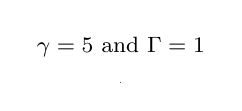
\begin{tikzpicture}[%
font=\footnotesize
]

\begin{axis}[%
width=0.951\figwidth,
height=\figheight,
at={(0\figwidth,0\figheight)},
scale only axis,
xmin=0,
xmax=3,
tick align=outside,
xlabel={Log-Moneyness},
xmajorgrids,
ymin=0,
ymax=5,
ylabel={Remaining Time},
ymajorgrids,
zmin=0,
zmax=0.4,
zlabel={Relative Increase},
zmajorgrids,
view={50}{40},
axis background/.style={fill=white},
title={$\gamma = 5$ and $\Gamma = 1$},
axis x line*=bottom,
axis y line*=left,
axis z line*=left
]

\addplot3[%
surf,
shader=flat corner,draw=black,z buffer=sort,colormap={mymap}{[1pt] rgb(0pt)=(0.2081,0.1663,0.5292); rgb(1pt)=(0.211624,0.189781,0.577676); rgb(2pt)=(0.212252,0.213771,0.626971); rgb(3pt)=(0.2081,0.2386,0.677086); rgb(4pt)=(0.195905,0.264457,0.7279); rgb(5pt)=(0.170729,0.291938,0.779248); rgb(6pt)=(0.125271,0.324243,0.830271); rgb(7pt)=(0.0591333,0.359833,0.868333); rgb(8pt)=(0.0116952,0.38751,0.881957); rgb(9pt)=(0.00595714,0.408614,0.882843); rgb(10pt)=(0.0165143,0.4266,0.878633); rgb(11pt)=(0.0328524,0.443043,0.871957); rgb(12pt)=(0.0498143,0.458571,0.864057); rgb(13pt)=(0.0629333,0.47369,0.855438); rgb(14pt)=(0.0722667,0.488667,0.8467); rgb(15pt)=(0.0779429,0.503986,0.838371); rgb(16pt)=(0.0793476,0.520024,0.831181); rgb(17pt)=(0.0749429,0.537543,0.826271); rgb(18pt)=(0.0640571,0.556986,0.823957); rgb(19pt)=(0.0487714,0.577224,0.822829); rgb(20pt)=(0.0343429,0.596581,0.819852); rgb(21pt)=(0.0265,0.6137,0.8135); rgb(22pt)=(0.0238905,0.628662,0.803762); rgb(23pt)=(0.0230905,0.641786,0.791267); rgb(24pt)=(0.0227714,0.653486,0.776757); rgb(25pt)=(0.0266619,0.664195,0.760719); rgb(26pt)=(0.0383714,0.674271,0.743552); rgb(27pt)=(0.0589714,0.683757,0.725386); rgb(28pt)=(0.0843,0.692833,0.706167); rgb(29pt)=(0.113295,0.7015,0.685857); rgb(30pt)=(0.145271,0.709757,0.664629); rgb(31pt)=(0.180133,0.717657,0.642433); rgb(32pt)=(0.217829,0.725043,0.619262); rgb(33pt)=(0.258643,0.731714,0.595429); rgb(34pt)=(0.302171,0.737605,0.571186); rgb(35pt)=(0.348167,0.742433,0.547267); rgb(36pt)=(0.395257,0.7459,0.524443); rgb(37pt)=(0.44201,0.748081,0.503314); rgb(38pt)=(0.487124,0.749062,0.483976); rgb(39pt)=(0.530029,0.749114,0.466114); rgb(40pt)=(0.570857,0.748519,0.44939); rgb(41pt)=(0.609852,0.747314,0.433686); rgb(42pt)=(0.6473,0.7456,0.4188); rgb(43pt)=(0.683419,0.743476,0.404433); rgb(44pt)=(0.71841,0.741133,0.390476); rgb(45pt)=(0.752486,0.7384,0.376814); rgb(46pt)=(0.785843,0.735567,0.363271); rgb(47pt)=(0.818505,0.732733,0.34979); rgb(48pt)=(0.850657,0.7299,0.336029); rgb(49pt)=(0.882433,0.727433,0.3217); rgb(50pt)=(0.913933,0.725786,0.306276); rgb(51pt)=(0.944957,0.726114,0.288643); rgb(52pt)=(0.973895,0.731395,0.266648); rgb(53pt)=(0.993771,0.745457,0.240348); rgb(54pt)=(0.999043,0.765314,0.216414); rgb(55pt)=(0.995533,0.786057,0.196652); rgb(56pt)=(0.988,0.8066,0.179367); rgb(57pt)=(0.978857,0.827143,0.163314); rgb(58pt)=(0.9697,0.848138,0.147452); rgb(59pt)=(0.962586,0.870514,0.1309); rgb(60pt)=(0.958871,0.8949,0.113243); rgb(61pt)=(0.959824,0.921833,0.0948381); rgb(62pt)=(0.9661,0.951443,0.0755333); rgb(63pt)=(0.9763,0.9831,0.0538)},mesh/rows=25]
table[row sep=crcr, point meta=\thisrow{c}] {%
%
x	y	z	c\\
0	0.01	0.0217171658131754	0.0217171658131754\\
0	0.111836734693878	0.111117593076313	0.111117593076313\\
0	0.213673469387755	0.185694161164657	0.185694161164657\\
0	0.315510204081633	0.24435852129021	0.24435852129021\\
0	0.41734693877551	0.286995080141692	0.286995080141692\\
0	0.519183673469388	0.316708278203502	0.316708278203502\\
0	0.621020408163265	0.337034445831762	0.337034445831762\\
0	0.722857142857143	0.350863276837653	0.350863276837653\\
0	0.82469387755102	0.360284107279394	0.360284107279394\\
0	0.926530612244898	0.366731070659999	0.366731070659999\\
0	1.02836734693878	0.371168324329704	0.371168324329704\\
0	1.13020408163265	0.37424048876166	0.37424048876166\\
0	1.23204081632653	0.376379435754066	0.376379435754066\\
0	1.33387755102041	0.377876147553436	0.377876147553436\\
0	1.43571428571429	0.378928079718796	0.378928079718796\\
0	1.53755102040816	0.379670217171989	0.379670217171989\\
0	1.63938775510204	0.380195492629651	0.380195492629651\\
0	1.74122448979592	0.380568300164557	0.380568300164557\\
0	1.8430612244898	0.380833513872084	0.380833513872084\\
0	1.94489795918367	0.381022560107687	0.381022560107687\\
0	2.04673469387755	0.38115754118623	0.38115754118623\\
0	2.14857142857143	0.381254058221745	0.381254058221745\\
0	2.25040816326531	0.381323157377029	0.381323157377029\\
0	2.35224489795918	0.381372680227943	0.381372680227943\\
0	2.45408163265306	0.38140820583384	0.38140820583384\\
0	2.55591836734694	0.381433711065724	0.381433711065724\\
0	2.65775510204082	0.381452035316954	0.381452035316954\\
0	2.75959183673469	0.381465208673571	0.381465208673571\\
0	2.86142857142857	0.381474684334305	0.381474684334305\\
0	2.96326530612245	0.381481503631342	0.381481503631342\\
0	3.06510204081633	0.381486413441215	0.381486413441215\\
0	3.1669387755102	0.381489949876146	0.381489949876146\\
0	3.26877551020408	0.381492498033704	0.381492498033704\\
0	3.37061224489796	0.381494334708112	0.381494334708112\\
0	3.47244897959184	0.381495658960581	0.381495658960581\\
0	3.57428571428571	0.381496614021753	0.381496614021753\\
0	3.67612244897959	0.381497302997415	0.381497302997415\\
0	3.77795918367347	0.381497800138675	0.381497800138675\\
0	3.87979591836735	0.381498158938092	0.381498158938092\\
0	3.98163265306122	0.381498417945394	0.381498417945394\\
0	4.0834693877551	0.38149860495152	0.38149860495152\\
0	4.18530612244898	0.38149873999555	0.38149873999555\\
0	4.28714285714286	0.38149883753217	0.38149883753217\\
0	4.38897959183674	0.3814989079901	0.3814989079901\\
0	4.49081632653061	0.381498958893813	0.381498958893813\\
0	4.59265306122449	0.381498995675455	0.381498995675455\\
0	4.69448979591837	0.381499022256506	0.381499022256506\\
0	4.79632653061224	0.381499041467826	0.381499041467826\\
0	4.89816326530612	0.381499055354689	0.381499055354689\\
0	5	0.381499065393684	0.381499065393684\\
0.125	0.01	0.000108922569071374	0.000108922569071374\\
0.125	0.111836734693878	0.0319874082245827	0.0319874082245827\\
0.125	0.213673469387755	0.0732475813625421	0.0732475813625421\\
0.125	0.315510204081633	0.110354189971304	0.110354189971304\\
0.125	0.41734693877551	0.139846962747464	0.139846962747464\\
0.125	0.519183673469388	0.161830807421706	0.161830807421706\\
0.125	0.621020408163265	0.177686477961597	0.177686477961597\\
0.125	0.722857142857143	0.188940367205693	0.188940367205693\\
0.125	0.82469387755102	0.196872749676949	0.196872749676949\\
0.125	0.926530612244898	0.202451976195808	0.202451976195808\\
0.125	1.02836734693878	0.206377391398988	0.206377391398988\\
0.125	1.13020408163265	0.209143433725675	0.209143433725675\\
0.125	1.23204081632653	0.211096495410224	0.211096495410224\\
0.125	1.33387755102041	0.212478535014668	0.212478535014668\\
0.125	1.43571428571429	0.213458597480406	0.213458597480406\\
0.125	1.53755102040816	0.214154995108134	0.214154995108134\\
0.125	1.63938775510204	0.214650737380111	0.214650737380111\\
0.125	1.74122448979592	0.215004222025675	0.215004222025675\\
0.125	1.8430612244898	0.215256642333757	0.215256642333757\\
0.125	1.94489795918367	0.215437129482254	0.215437129482254\\
0.125	2.04673469387755	0.215566332305689	0.215566332305689\\
0.125	2.14857142857143	0.215658918117557	0.215658918117557\\
0.125	2.25040816326531	0.215725325035522	0.215725325035522\\
0.125	2.35224489795918	0.215772993886531	0.215772993886531\\
0.125	2.45408163265306	0.215807236757549	0.215807236757549\\
0.125	2.55591836734694	0.215831851064646	0.215831851064646\\
0.125	2.65775510204082	0.215849554627827	0.215849554627827\\
0.125	2.75959183673469	0.215862293682928	0.215862293682928\\
0.125	2.86142857142857	0.21587146532095	0.21587146532095\\
0.125	2.96326530612245	0.215878071193392	0.215878071193392\\
0.125	3.06510204081633	0.215882830912707	0.215882830912707\\
0.125	3.1669387755102	0.21588626163409	0.21588626163409\\
0.125	3.26877551020408	0.215888735233232	0.215888735233232\\
0.125	3.37061224489796	0.215890519259668	0.215890519259668\\
0.125	3.47244897959184	0.215891806296479	0.215891806296479\\
0.125	3.57428571428571	0.215892735025709	0.215892735025709\\
0.125	3.67612244897959	0.215893405353816	0.215893405353816\\
0.125	3.77795918367347	0.215893889279249	0.215893889279249\\
0.125	3.87979591836735	0.215894238705397	0.215894238705397\\
0.125	3.98163265306122	0.215894491060515	0.215894491060515\\
0.125	4.0834693877551	0.215894673342154	0.215894673342154\\
0.125	4.18530612244898	0.215894805029054	0.215894805029054\\
0.125	4.28714285714286	0.21589490017848	0.21589490017848\\
0.125	4.38897959183674	0.215894968937424	0.215894968937424\\
0.125	4.49081632653061	0.215895018631834	0.215895018631834\\
0.125	4.59265306122449	0.215895054551941	0.215895054551941\\
0.125	4.69448979591837	0.215895080518638	0.215895080518638\\
0.125	4.79632653061224	0.21589509929206	0.21589509929206\\
0.125	4.89816326530612	0.215895112866393	0.215895112866393\\
0.125	5	0.215895122682648	0.215895122682648\\
0.25	0.01	3.04311503618577e-09	3.04311503618577e-09\\
0.25	0.111836734693878	0.00667951807656567	0.00667951807656567\\
0.25	0.213673469387755	0.0249862067882534	0.0249862067882534\\
0.25	0.315510204081633	0.0456291563029526	0.0456291563029526\\
0.25	0.41734693877551	0.0641988350383688	0.0641988350383688\\
0.25	0.519183673469388	0.0792664580065087	0.0792664580065087\\
0.25	0.621020408163265	0.0908455249729353	0.0908455249729353\\
0.25	0.722857142857143	0.0994799210919912	0.0994799210919912\\
0.25	0.82469387755102	0.105809436931347	0.105809436931347\\
0.25	0.926530612244898	0.11040393315318	0.11040393315318\\
0.25	1.02836734693878	0.113720133849158	0.113720133849158\\
0.25	1.13020408163265	0.116105979277837	0.116105979277837\\
0.25	1.23204081632653	0.117819469671305	0.117819469671305\\
0.25	1.33387755102041	0.119049029923362	0.119049029923362\\
0.25	1.43571428571429	0.119931069478986	0.119931069478986\\
0.25	1.53755102040816	0.12056383877371	0.12056383877371\\
0.25	1.63938775510204	0.121017898031592	0.121017898031592\\
0.25	1.74122448979592	0.121343841796568	0.121343841796568\\
0.25	1.8430612244898	0.121577922426078	0.121577922426078\\
0.25	1.94489795918367	0.121746110006856	0.121746110006856\\
0.25	2.04673469387755	0.121867011427999	0.121867011427999\\
0.25	2.14857142857143	0.121953962453627	0.121953962453627\\
0.25	2.25040816326531	0.122016525319413	0.122016525319413\\
0.25	2.35224489795918	0.122061560060122	0.122061560060122\\
0.25	2.45408163265306	0.122093990817963	0.122093990817963\\
0.25	2.55591836734694	0.12211735409526	0.12211735409526\\
0.25	2.65775510204082	0.12213419172847	0.12213419172847\\
0.25	2.75959183673469	0.122146329095157	0.122146329095157\\
0.25	2.86142857142857	0.12215508211067	0.12215508211067\\
0.25	2.96326530612245	0.122161395988125	0.122161395988125\\
0.25	3.06510204081633	0.122165951644421	0.122165951644421\\
0.25	3.1669387755102	0.122169239507859	0.122169239507859\\
0.25	3.26877551020408	0.122171612940571	0.122171612940571\\
0.25	3.37061224489796	0.122173326634852	0.122173326634852\\
0.25	3.47244897959184	0.122174564224179	0.122174564224179\\
0.25	3.57428571428571	0.122175458148162	0.122175458148162\\
0.25	3.67612244897959	0.122176103951014	0.122176103951014\\
0.25	3.77795918367347	0.122176570577711	0.122176570577711\\
0.25	3.87979591836735	0.122176907791029	0.122176907791029\\
0.25	3.98163265306122	0.122177151516482	0.122177151516482\\
0.25	4.0834693877551	0.122177327695349	0.122177327695349\\
0.25	4.18530612244898	0.122177455063062	0.122177455063062\\
0.25	4.28714285714286	0.122177547153278	0.122177547153278\\
0.25	4.38897959183674	0.12217761374379	0.12217761374379\\
0.25	4.49081632653061	0.122177661900011	0.122177661900011\\
0.25	4.59265306122449	0.122177696728185	0.122177696728185\\
0.25	4.69448979591837	0.122177721919193	0.122177721919193\\
0.25	4.79632653061224	0.122177740141257	0.122177740141257\\
0.25	4.89816326530612	0.122177753323553	0.122177753323553\\
0.25	5	0.122177762861098	0.122177762861098\\
0.375	0.01	2.47887919007473e-16	2.47887919007473e-16\\
0.375	0.111836734693878	0.000946611229225926	0.000946611229225926\\
0.375	0.213673469387755	0.00716740951731688	0.00716740951731688\\
0.375	0.315510204081633	0.0169911894583221	0.0169911894583221\\
0.375	0.41734693877551	0.0274449135830357	0.0274449135830357\\
0.375	0.519183673469388	0.0368872128571661	0.0368872128571661\\
0.375	0.621020408163265	0.0447226196500155	0.0447226196500155\\
0.375	0.722857142857143	0.0509165482044067	0.0509165482044067\\
0.375	0.82469387755102	0.055670161361601	0.055670161361601\\
0.375	0.926530612244898	0.0592501179174284	0.0592501179174284\\
0.375	1.02836734693878	0.0619126589204712	0.0619126589204712\\
0.375	1.13020408163265	0.0638760563000532	0.0638760563000532\\
0.375	1.23204081632653	0.0653153089196266	0.0653153089196266\\
0.375	1.33387755102041	0.0663659110200529	0.0663659110200529\\
0.375	1.43571428571429	0.0671305109768868	0.0671305109768868\\
0.375	1.53755102040816	0.0676857681626808	0.0676857681626808\\
0.375	1.63938775510204	0.0680883769142378	0.0680883769142378\\
0.375	1.74122448979592	0.0683799813264616	0.0683799813264616\\
0.375	1.8430612244898	0.0685910229020684	0.0685910229020684\\
0.375	1.94489795918367	0.0687436771511779	0.0687436771511779\\
0.375	2.04673469387755	0.0688540578952594	0.0688540578952594\\
0.375	2.14857142857143	0.0689338532707918	0.0689338532707918\\
0.375	2.25040816326531	0.0689915303945139	0.0689915303945139\\
0.375	2.35224489795918	0.0690332174545072	0.0690332174545072\\
0.375	2.45408163265306	0.0690633470125448	0.0690633470125448\\
0.375	2.55591836734694	0.0690851238134695	0.0690851238134695\\
0.375	2.65775510204082	0.0691008642262636	0.0691008642262636\\
0.375	2.75959183673469	0.069112242248823	0.069112242248823\\
0.375	2.86142857142857	0.0691204675392279	0.0691204675392279\\
0.375	2.96326530612245	0.0691264141942802	0.0691264141942802\\
0.375	3.06510204081633	0.0691307138451774	0.0691307138451774\\
0.375	3.1669387755102	0.0691338229362807	0.0691338229362807\\
0.375	3.26877551020408	0.0691360713365558	0.0691360713365558\\
0.375	3.37061224489796	0.0691376974593452	0.0691376974593452\\
0.375	3.47244897959184	0.0691388737270534	0.0691388737270534\\
0.375	3.57428571428571	0.0691397245612686	0.0691397245612686\\
0.375	3.67612244897959	0.0691403399244226	0.0691403399244226\\
0.375	3.77795918367347	0.0691407852202224	0.0691407852202224\\
0.375	3.87979591836735	0.0691411074089923	0.0691411074089923\\
0.375	3.98163265306122	0.0691413405424988	0.0691413405424988\\
0.375	4.0834693877551	0.0691415092483396	0.0691415092483396\\
0.375	4.18530612244898	0.0691416313398083	0.0691416313398083\\
0.375	4.28714285714286	0.0691417197025081	0.0691417197025081\\
0.375	4.38897959183674	0.0691417836582915	0.0691417836582915\\
0.375	4.49081632653061	0.0691418299514311	0.0691418299514311\\
0.375	4.59265306122449	0.0691418634617252	0.0691418634617252\\
0.375	4.69448979591837	0.0691418877202014	0.0691418877202014\\
0.375	4.79632653061224	0.0691419052820979	0.0691419052820979\\
0.375	4.89816326530612	0.069141917996645	0.069141917996645\\
0.375	5	0.0691419272022217	0.0691419272022217\\
0.5	0.01	4.77949431892059e-26	4.77949431892059e-26\\
0.5	0.111836734693878	8.6638981729131e-05	8.6638981729131e-05\\
0.5	0.213673469387755	0.00168698073736829	0.00168698073736829\\
0.5	0.315510204081633	0.00561209863100597	0.00561209863100597\\
0.5	0.41734693877551	0.0108072733334969	0.0108072733334969\\
0.5	0.519183673469388	0.0161698356265338	0.0161698356265338\\
0.5	0.621020408163265	0.0210513061144946	0.0210513061144946\\
0.5	0.722857142857143	0.025185427910498	0.025185427910498\\
0.5	0.82469387755102	0.0285328213531547	0.0285328213531547\\
0.5	0.926530612244898	0.0311640793582405	0.0311640793582405\\
0.5	1.02836734693878	0.0331906010090201	0.0331906010090201\\
0.5	1.13020408163265	0.0347288059405313	0.0347288059405313\\
0.5	1.23204081632653	0.03588397873502	0.03588397873502\\
0.5	1.33387755102041	0.0367446191156378	0.0367446191156378\\
0.5	1.43571428571429	0.0373819638459519	0.0373819638459519\\
0.5	1.53755102040816	0.0378517666828212	0.0378517666828212\\
0.5	1.63938775510204	0.0381968309539886	0.0381968309539886\\
0.5	1.74122448979592	0.0384495691172589	0.0384495691172589\\
0.5	1.8430612244898	0.0386342791165429	0.0386342791165429\\
0.5	1.94489795918367	0.0387690390698139	0.0387690390698139\\
0.5	2.04673469387755	0.0388672226799385	0.0388672226799385\\
0.5	2.14857142857143	0.0389386800838239	0.0389386800838239\\
0.5	2.25040816326531	0.038990641565943	0.038990641565943\\
0.5	2.35224489795918	0.0390284003016058	0.0390284003016058\\
0.5	2.45408163265306	0.03905582328401	0.03905582328401\\
0.5	2.55591836734694	0.0390757309618348	0.0390757309618348\\
0.5	2.65775510204082	0.0390901778020951	0.0390901778020951\\
0.5	2.75959183673469	0.0391006587738927	0.0391006587738927\\
0.5	2.86142857142857	0.0391082608238778	0.0391082608238778\\
0.5	2.96326530612245	0.0391137737187451	0.0391137737187451\\
0.5	3.06510204081633	0.0391177709944066	0.0391177709944066\\
0.5	3.1669387755102	0.0391206689817173	0.0391206689817173\\
0.5	3.26877551020408	0.0391227697930985	0.0391227697930985\\
0.5	3.37061224489796	0.0391242925975851	0.0391242925975851\\
0.5	3.47244897959184	0.0391253963572024	0.0391253963572024\\
0.5	3.57428571428571	0.0391261963454855	0.0391261963454855\\
0.5	3.67612244897959	0.0391267761425107	0.0391267761425107\\
0.5	3.77795918367347	0.0391271963416217	0.0391271963416217\\
0.5	3.87979591836735	0.0391275008672304	0.0391275008672304\\
0.5	3.98163265306122	0.0391277215579422	0.0391277215579422\\
0.5	4.0834693877551	0.0391278814905826	0.0391278814905826\\
0.5	4.18530612244898	0.0391279973906104	0.0391279973906104\\
0.5	4.28714285714286	0.0391280813796455	0.0391280813796455\\
0.5	4.38897959183674	0.0391281422476914	0.0391281422476914\\
0.5	4.49081632653061	0.0391281863577133	0.0391281863577133\\
0.5	4.59265306122449	0.0391282183235174	0.0391282183235174\\
0.5	4.69448979591837	0.0391282414886651	0.0391282414886651\\
0.5	4.79632653061224	0.0391282582761686	0.0391282582761686\\
0.5	4.89816326530612	0.0391282704419265	0.0391282704419265\\
0.5	5	0.0391282792583933	0.0391282792583933\\
0.625	0.01	2.00413903262261e-38	2.00413903262261e-38\\
0.625	0.111836734693878	4.9478459668759e-06	4.9478459668759e-06\\
0.625	0.213673469387755	0.000319268839366317	0.000319268839366317\\
0.625	0.315510204081633	0.00162225088738685	0.00162225088738685\\
0.625	0.41734693877551	0.00388133875539428	0.00388133875539428\\
0.625	0.519183673469388	0.00662420860164469	0.00662420860164469\\
0.625	0.621020408163265	0.00941177969549677	0.00941177969549677\\
0.625	0.722857142857143	0.0119710061878386	0.0119710061878386\\
0.625	0.82469387755102	0.014175994388697	0.014175994388697\\
0.625	0.926530612244898	0.0159970488671258	0.0159970488671258\\
0.625	1.02836734693878	0.0174571781902701	0.0174571781902701\\
0.625	1.13020408163265	0.0186030742995102	0.0186030742995102\\
0.625	1.23204081632653	0.0194880981053415	0.0194880981053415\\
0.625	1.33387755102041	0.0201633634248122	0.0201633634248122\\
0.625	1.43571428571429	0.0206737453335693	0.0206737453335693\\
0.625	1.53755102040816	0.0210566564060745	0.0210566564060745\\
0.625	1.63938775510204	0.0213422485780574	0.0213422485780574\\
0.625	1.74122448979592	0.0215542550155561	0.0215542550155561\\
0.625	1.8430612244898	0.0217110387119245	0.0217110387119245\\
0.625	1.94489795918367	0.0218266263420195	0.0218266263420195\\
0.625	2.04673469387755	0.021911627570043	0.021911627570043\\
0.625	2.14857142857143	0.0219740064257551	0.0219740064257551\\
0.625	2.25040816326531	0.0220197051708049	0.0220197051708049\\
0.625	2.35224489795918	0.0220531363593128	0.0220531363593128\\
0.625	2.45408163265306	0.0220775640346679	0.0220775640346679\\
0.625	2.55591836734694	0.022095395145115	0.022095395145115\\
0.625	2.65775510204082	0.0221084000922219	0.0221084000922219\\
0.625	2.75959183673469	0.0221178783527324	0.0221178783527324\\
0.625	2.86142857142857	0.0221247820968621	0.0221247820968621\\
0.625	2.96326530612245	0.022129808010071	0.022129808010071\\
0.625	3.06510204081633	0.0221334652326279	0.0221334652326279\\
0.625	3.1669387755102	0.0221361254709285	0.0221361254709285\\
0.625	3.26877551020408	0.0221380598643811	0.0221380598643811\\
0.625	3.37061224489796	0.0221394660513617	0.0221394660513617\\
0.625	3.47244897959184	0.0221404880052426	0.0221404880052426\\
0.625	3.57428571428571	0.0221412305507463	0.0221412305507463\\
0.625	3.67612244897959	0.0221417699744098	0.0221417699744098\\
0.625	3.77795918367347	0.0221421617722116	0.0221421617722116\\
0.625	3.87979591836735	0.0221424463019167	0.0221424463019167\\
0.625	3.98163265306122	0.0221426529037702	0.0221426529037702\\
0.625	4.0834693877551	0.0221428029027014	0.0221428029027014\\
0.625	4.18530612244898	0.0221429117944565	0.0221429117944565\\
0.625	4.28714285714286	0.0221429908367518	0.0221429908367518\\
0.625	4.38897959183674	0.0221430482069109	0.0221430482069109\\
0.625	4.49081632653061	0.0221430898438061	0.0221430898438061\\
0.625	4.59265306122449	0.0221431200600098	0.0221431200600098\\
0.625	4.69448979591837	0.0221431419867516	0.0221431419867516\\
0.625	4.79632653061224	0.0221431578972714	0.0221431578972714\\
0.625	4.89816326530612	0.0221431694417523	0.0221431694417523\\
0.625	5	0.0221431778179799	0.0221431778179799\\
0.75	0.01	1.75330482033327e-53	1.75330482033327e-53\\
0.75	0.111836734693878	1.72245392220561e-07	1.72245392220561e-07\\
0.75	0.213673469387755	4.78154858387409e-05	4.78154858387409e-05\\
0.75	0.315510204081633	0.000405732245256072	0.000405732245256072\\
0.75	0.41734693877551	0.0012602414355673	0.0012602414355673\\
0.75	0.519183673469388	0.00251798250220281	0.00251798250220281\\
0.75	0.621020408163265	0.00397236255608428	0.00397236255608428\\
0.75	0.722857142857143	0.00543843810445796	0.00543843810445796\\
0.75	0.82469387755102	0.00679495984740543	0.00679495984740543\\
0.75	0.926530612244898	0.00798032964682199	0.00798032964682199\\
0.75	1.02836734693878	0.00897536389688323	0.00897536389688323\\
0.75	1.13020408163265	0.00978650780540177	0.00978650780540177\\
0.75	1.23204081632653	0.0104333504197824	0.0104333504197824\\
0.75	1.33387755102041	0.0109405184281499	0.0109405184281499\\
0.75	1.43571428571429	0.0113329417842514	0.0113329417842514\\
0.75	1.53755102040816	0.011633405569264	0.011633405569264\\
0.75	1.63938775510204	0.0118615243667572	0.0118615243667572\\
0.75	1.74122448979592	0.0120335342025705	0.0120335342025705\\
0.75	1.8430612244898	0.0121625103218443	0.0121625103218443\\
0.75	1.94489795918367	0.0122587726854946	0.0122587726854946\\
0.75	2.04673469387755	0.0123303435235074	0.0123303435235074\\
0.75	2.14857142857143	0.0123833858617989	0.0123833858617989\\
0.75	2.25040816326531	0.012422590624374	0.012422590624374\\
0.75	2.35224489795918	0.0124515018332293	0.0124515018332293\\
0.75	2.45408163265306	0.0124727809698636	0.0124727809698636\\
0.75	2.55591836734694	0.0124884169491109	0.0124884169491109\\
0.75	2.65775510204082	0.0124998900681844	0.0124998900681844\\
0.75	2.75959183673469	0.0125082983691649	0.0125082983691649\\
0.75	2.86142857142857	0.0125144540555952	0.0125144540555952\\
0.75	2.96326530612245	0.0125189564761682	0.0125189564761682\\
0.75	3.06510204081633	0.0125222470186785	0.0125222470186785\\
0.75	3.1669387755102	0.0125246501842739	0.0125246501842739\\
0.75	3.26877551020408	0.0125264041905968	0.0125264041905968\\
0.75	3.37061224489796	0.0125276836930099	0.0125276836930099\\
0.75	3.47244897959184	0.0125286166043715	0.0125286166043715\\
0.75	3.57428571428571	0.0125292965154134	0.0125292965154134\\
0.75	3.67612244897959	0.012529791847262	0.012529791847262\\
0.75	3.77795918367347	0.0125301525838861	0.0125301525838861\\
0.75	3.87979591836735	0.0125304152168254	0.0125304152168254\\
0.75	3.98163265306122	0.0125306063721399	0.0125306063721399\\
0.75	4.0834693877551	0.0125307454677478	0.0125307454677478\\
0.75	4.18530612244898	0.0125308466584383	0.0125308466584383\\
0.75	4.28714285714286	0.0125309202582759	0.0125309202582759\\
0.75	4.38897959183674	0.0125309737800291	0.0125309737800291\\
0.75	4.49081632653061	0.0125310126942305	0.0125310126942305\\
0.75	4.59265306122449	0.0125310409831656	0.0125310409831656\\
0.75	4.69448979591837	0.0125310615449811	0.0125310615449811\\
0.75	4.79632653061224	0.0125310764883258	0.0125310764883258\\
0.75	4.89816326530612	0.0125310873470863	0.0125310873470863\\
0.75	5	0.01253109523683	0.01253109523683\\
0.875	0.01	3.1267479456744e-71	3.1267479456744e-71\\
0.875	0.111836734693878	3.59761941412949e-09	3.59761941412949e-09\\
0.875	0.213673469387755	5.59772560625297e-06	5.59772560625297e-06\\
0.875	0.315510204081633	8.69710726747009e-05	8.69710726747009e-05\\
0.875	0.41734693877551	0.000367153984941842	0.000367153984941842\\
0.875	0.519183673469388	0.00088250093709678	0.00088250093709678\\
0.875	0.621020408163265	0.00157405775975653	0.00157405775975653\\
0.875	0.722857142857143	0.00234987939396778	0.00234987939396778\\
0.875	0.82469387755102	0.00312833989403652	0.00312833989403652\\
0.875	0.926530612244898	0.00385341831943349	0.00385341831943349\\
0.875	1.02836734693878	0.00449437008279354	0.00449437008279354\\
0.875	1.13020408163265	0.00503971461874203	0.00503971461874203\\
0.875	1.23204081632653	0.00549054449359006	0.00549054449359006\\
0.875	1.33387755102041	0.00585505033900051	0.00585505033900051\\
0.875	1.43571428571429	0.0061446552543097	0.0061446552543097\\
0.875	1.53755102040816	0.00637156049576111	0.00637156049576111\\
0.875	1.63938775510204	0.00654734428091729	0.00654734428091729\\
0.875	1.74122448979592	0.00668227274199712	0.00668227274199712\\
0.875	1.8430612244898	0.00678505551546572	0.00678505551546572\\
0.875	1.94489795918367	0.00686285667127799	0.00686285667127799\\
0.875	2.04673469387755	0.00692143642626741	0.00692143642626741\\
0.875	2.14857142857143	0.00696534674504236	0.00696534674504236\\
0.875	2.25040816326531	0.00699813651366308	0.00699813651366308\\
0.875	2.35224489795918	0.00702254300746944	0.00702254300746944\\
0.875	2.45408163265306	0.00704065925653353	0.00704065925653353\\
0.875	2.55591836734694	0.00705407435366049	0.00705407435366049\\
0.875	2.65775510204082	0.00706398772723518	0.00706398772723518\\
0.875	2.75959183673469	0.00707130027007319	0.00707130027007319\\
0.875	2.86142857142857	0.00707668586407024	0.00707668586407024\\
0.875	2.96326530612245	0.00708064682846296	0.00708064682846296\\
0.875	3.06510204081633	0.00708355648598361	0.00708355648598361\\
0.875	3.1669387755102	0.00708569158264775	0.00708569158264775\\
0.875	3.26877551020408	0.00708725682084077	0.00708725682084077\\
0.875	3.37061224489796	0.00708840332547195	0.00708840332547195\\
0.875	3.47244897959184	0.00708924248173111	0.00708924248173111\\
0.875	3.57428571428571	0.00708985626568577	0.00708985626568577\\
0.875	3.67612244897959	0.00709030493208655	0.00709030493208655\\
0.875	3.77795918367347	0.00709063271992052	0.00709063271992052\\
0.875	3.87979591836735	0.00709087207692914	0.00709087207692914\\
0.875	3.98163265306122	0.00709104678121231	0.00709104678121231\\
0.875	4.0834693877551	0.00709117424380677	0.00709117424380677\\
0.875	4.18530612244898	0.00709126720451998	0.00709126720451998\\
0.875	4.28714285714286	0.0070913349792159	0.0070913349792159\\
0.875	4.38897959183674	0.00709138437610232	0.00709138437610232\\
0.875	4.49081632653061	0.00709142036814938	0.00709142036814938\\
0.875	4.59265306122449	0.00709144658608223	0.00709144658608223\\
0.875	4.69448979591837	0.00709146567952356	0.00709146567952356\\
0.875	4.79632653061224	0.00709147958135093	0.00709147958135093\\
0.875	4.89816326530612	0.00709148970107679	0.00709148970107679\\
0.875	5	0.00709149706622266	0.00709149706622266\\
1	0.01	1.1206262581765e-91	1.1206262581765e-91\\
1	0.111836734693878	4.45908694918491e-11	4.45908694918491e-11\\
1	0.213673469387755	5.0748810856876e-07	5.0748810856876e-07\\
1	0.315510204081633	1.58552008508997e-05	1.58552008508997e-05\\
1	0.41734693877551	9.53623261794575e-05	9.53623261794575e-05\\
1	0.519183673469388	0.000283617180570505	0.000283617180570505\\
1	0.621020408163265	0.00058273742303869	0.00058273742303869\\
1	0.722857142857143	0.000961448940881388	0.000961448940881388\\
1	0.82469387755102	0.00137774168028923	0.00137774168028923\\
1	0.926530612244898	0.00179423908163292	0.00179423908163292\\
1	1.02836734693878	0.00218430745517906	0.00218430745517906\\
1	1.13020408163265	0.00253241301688541	0.00253241301688541\\
1	1.23204081632653	0.00283196943944286	0.00283196943944286\\
1	1.33387755102041	0.00308259845866974	0.00308259845866974\\
1	1.43571428571429	0.00328769233406285	0.00328769233406285\\
1	1.53755102040816	0.00345256785159323	0.00345256785159323\\
1	1.63938775510204	0.00358321264805126	0.00358321264805126\\
1	1.74122448979592	0.00368551388838047	0.00368551388838047\\
1	1.8430612244898	0.00376483738047146	0.00376483738047146\\
1	1.94489795918367	0.0038258408088738	0.0038258408088738\\
1	2.04673469387755	0.00387243166565164	0.00387243166565164\\
1	2.14857142857143	0.00390780680070011	0.00390780680070011\\
1	2.25040816326531	0.00393453198802457	0.00393453198802457\\
1	2.35224489795918	0.00395463576007412	0.00395463576007412\\
1	2.45408163265306	0.00396970270275456	0.00396970270275456\\
1	2.55591836734694	0.00398095854631119	0.00398095854631119\\
1	2.65775510204082	0.00398934380801224	0.00398934380801224\\
1	2.75959183673469	0.00399557531695606	0.00399557531695606\\
1	2.86142857142857	0.00400019633019756	0.00400019633019756\\
1	2.96326530612245	0.0040036165886151	0.0040036165886151\\
1	3.06510204081633	0.00400614386562957	0.00400614386562957\\
1	3.1669387755102	0.00400800852829321	0.00400800852829321\\
1	3.26877551020408	0.0040093824797466	0.0040093824797466\\
1	3.37061224489796	0.00401039365636755	0.00401039365636755\\
1	3.47244897959184	0.00401113705214979	0.00401113705214979\\
1	3.57428571428571	0.00401168305738548	0.00401168305738548\\
1	3.67612244897959	0.00401208373735716	0.00401208373735716\\
1	3.77795918367347	0.00401237754165409	0.00401237754165409\\
1	3.87979591836735	0.00401259282463255	0.00401259282463255\\
1	3.98163265306122	0.00401275046956661	0.00401275046956661\\
1	4.0834693877551	0.00401286583978684	0.00401286583978684\\
1	4.18530612244898	0.00401295022623055	0.00401295022623055\\
1	4.28714285714286	0.00401301191930737	0.00401301191930737\\
1	4.38897959183674	0.00401305700122892	0.00401305700122892\\
1	4.49081632653061	0.00401308993081784	0.00401308993081784\\
1	4.59265306122449	0.00401311397456636	0.00401311397456636\\
1	4.69448979591837	0.00401313152398392	0.00401313152398392\\
1	4.79632653061224	0.00401314432897734	0.00401314432897734\\
1	4.89816326530612	0.00401315366931346	0.00401315366931346\\
1	5	0.00401316048048086	0.00401316048048086\\
1.125	0.01	7.99678373004361e-115	7.99678373004361e-115\\
1.125	0.111836734693878	3.25428714235603e-13	3.25428714235603e-13\\
1.125	0.213673469387755	3.53773806862332e-08	3.53773806862332e-08\\
1.125	0.315510204081633	2.44302565551252e-06	2.44302565551252e-06\\
1.125	0.41734693877551	2.19634616766623e-05	2.19634616766623e-05\\
1.125	0.519183673469388	8.31861302128006e-05	8.31861302128006e-05\\
1.125	0.621020408163265	0.000200704779298671	0.000200704779298671\\
1.125	0.722857142857143	0.000371035776215236	0.000371035776215236\\
1.125	0.82469387755102	0.000578308304618825	0.000578308304618825\\
1.125	0.926530612244898	0.00080283657967408	0.00080283657967408\\
1.125	1.02836734693878	0.00102701731731546	0.00102701731731546\\
1.125	1.13020408163265	0.0012379219474082	0.0012379219474082\\
1.125	1.23204081632653	0.00142763585228203	0.00142763585228203\\
1.125	1.33387755102041	0.00159247285217596	0.00159247285217596\\
1.125	1.43571428571429	0.001731828977592	0.001731828977592\\
1.125	1.53755102040816	0.00184708373398948	0.00184708373398948\\
1.125	1.63938775510204	0.00194071659896997	0.00194071659896997\\
1.125	1.74122448979592	0.00201567230080013	0.00201567230080013\\
1.125	1.8430612244898	0.00207494616016925	0.00207494616016925\\
1.125	1.94489795918367	0.00212133991788151	0.00212133991788151\\
1.125	2.04673469387755	0.00215733828235569	0.00215733828235569\\
1.125	2.14857142857143	0.00218506468447474	0.00218506468447474\\
1.125	2.25040816326531	0.00220628501219582	0.00220628501219582\\
1.125	2.35224489795918	0.00222243749860984	0.00222243749860984\\
1.125	2.45408163265306	0.00223467443945618	0.00223467443945618\\
1.125	2.55591836734694	0.00224390692788555	0.00224390692788555\\
1.125	2.65775510204082	0.00225084760334059	0.00225084760334059\\
1.125	2.75959183673469	0.00225604890763278	0.00225604890763278\\
1.125	2.86142857142857	0.00225993589133779	0.00225993589133779\\
1.125	2.96326530612245	0.00226283351612029	0.00226283351612029\\
1.125	3.06510204081633	0.0022649888775903	0.0022649888775903\\
1.125	3.1669387755102	0.00226658898772531	0.00226658898772531\\
1.125	3.26877551020408	0.00226777481365113	0.00226777481365113\\
1.125	3.37061224489796	0.00226865224105992	0.00226865224105992\\
1.125	3.47244897959184	0.00226930055992	0.00226930055992\\
1.125	3.57428571428571	0.00226977898387092	0.00226977898387092\\
1.125	3.67612244897959	0.00227013162775745	0.00227013162775745\\
1.125	3.77795918367347	0.00227039128784318	0.00227039128784318\\
1.125	3.87979591836735	0.0022705822996856	0.0022705822996856\\
1.125	3.98163265306122	0.00227072269024696	0.00227072269024696\\
1.125	4.0834693877551	0.00227082579301068	0.00227082579301068\\
1.125	4.18530612244898	0.00227090145648213	0.00227090145648213\\
1.125	4.28714285714286	0.00227095694607302	0.00227095694607302\\
1.125	4.38897959183674	0.00227099761560494	0.00227099761560494\\
1.125	4.49081632653061	0.00227102740625442	0.00227102740625442\\
1.125	4.59265306122449	0.00227104921660365	0.00227104921660365\\
1.125	4.69448979591837	0.00227106517664494	0.00227106517664494\\
1.125	4.79632653061224	0.00227107685036939	0.00227107685036939\\
1.125	4.89816326530612	0.00227108538535459	0.00227108538535459\\
1.125	5	0.00227109162308536	0.00227109162308536\\
1.25	0.01	1.12892475743399e-140	1.12892475743399e-140\\
1.25	0.111836734693878	1.3905482978089e-15	1.3905482978089e-15\\
1.25	0.213673469387755	1.88605219960152e-09	1.88605219960152e-09\\
1.25	0.315510204081633	3.1657426661299e-07	3.1657426661299e-07\\
1.25	0.41734693877551	4.46553513019678e-06	4.46553513019678e-06\\
1.25	0.519183673469388	2.21778156678447e-05	2.21778156678447e-05\\
1.25	0.621020408163265	6.40727904851969e-05	6.40727904851969e-05\\
1.25	0.722857142857143	0.000134592934180347	0.000134592934180347\\
1.25	0.82469387755102	0.00023060962689636	0.00023060962689636\\
1.25	0.926530612244898	0.000344143325370011	0.000344143325370011\\
1.25	1.02836734693878	0.000465769666917582	0.000465769666917582\\
1.25	1.13020408163265	0.000587017687800471	0.000587017687800471\\
1.25	1.23204081632653	0.000701512499514235	0.000701512499514235\\
1.25	1.33387755102041	0.000805195375483136	0.000805195375483136\\
1.25	1.43571428571429	0.000896033882448586	0.000896033882448586\\
1.25	1.53755102040816	0.000973533735111697	0.000973533735111697\\
1.25	1.63938775510204	0.00103823829767136	0.00103823829767136\\
1.25	1.74122448979592	0.00109130450386977	0.00109130450386977\\
1.25	1.8430612244898	0.00113418313369181	0.00113418313369181\\
1.25	1.94489795918367	0.00116839921337537	0.00116839921337537\\
1.25	2.04673469387755	0.0011954147239711	0.0011954147239711\\
1.25	2.14857142857143	0.00121655268861418	0.00121655268861418\\
1.25	2.25040816326531	0.00123296364133368	0.00123296364133368\\
1.25	2.35224489795918	0.00124561927522948	0.00124561927522948\\
1.25	2.45408163265306	0.00125532206532006	0.00125532206532006\\
1.25	2.55591836734694	0.00126272312768606	0.00126272312768606\\
1.25	2.65775510204082	0.0012683432861272	0.0012683432861272\\
1.25	2.75959183673469	0.0012725942923371	0.0012725942923371\\
1.25	2.86142857142857	0.00127579850673736	0.00127579850673736\\
1.25	2.96326530612245	0.00127820623817217	0.00127820623817217\\
1.25	3.06510204081633	0.00128001049264652	0.00128001049264652\\
1.25	3.1669387755102	0.00128135920024292	0.00128135920024292\\
1.25	3.26877551020408	0.00128236515510817	0.00128236515510817\\
1.25	3.37061224489796	0.00128311397301821	0.00128311397301821\\
1.25	3.47244897959184	0.00128367038358816	0.00128367038358816\\
1.25	3.57428571428571	0.00128408315545398	0.00128408315545398\\
1.25	3.67612244897959	0.00128438891902127	0.00128438891902127\\
1.25	3.77795918367347	0.00128461511251639	0.00128461511251639\\
1.25	3.87979591836735	0.0012847822386894	0.0012847822386894\\
1.25	3.98163265306122	0.00128490558449713	0.00128490558449713\\
1.25	4.0834693877551	0.00128499652566753	0.00128499652566753\\
1.25	4.18530612244898	0.00128506351247142	0.00128506351247142\\
1.25	4.28714285714286	0.0012851128120416	0.0012851128120416\\
1.25	4.38897959183674	0.00128514906566758	0.00128514906566758\\
1.25	4.49081632653061	0.00128517570605807	0.00128517570605807\\
1.25	4.59265306122449	0.00128519526900857	0.00128519526900857\\
1.25	4.69448979591837	0.00128520962569806	0.00128520962569806\\
1.25	4.79632653061224	0.0012852201554946	0.0012852201554946\\
1.25	4.89816326530612	0.00128522787428281	0.00128522787428281\\
1.25	5	0.00128523352961224	0.00128523352961224\\
1.375	0.01	3.13837007611789e-169	3.13837007611789e-169\\
1.375	0.111836734693878	3.46423200868573e-18	3.46423200868573e-18\\
1.375	0.213673469387755	7.65760591256092e-11	7.65760591256092e-11\\
1.375	0.315510204081633	3.43617864639403e-08	3.43617864639403e-08\\
1.375	0.41734693877551	7.98512435668517e-07	7.98512435668517e-07\\
1.375	0.519183673469388	5.35611917801158e-06	5.35611917801158e-06\\
1.375	0.621020408163265	1.88990842804822e-05	1.88990842804822e-05\\
1.375	0.722857142857143	4.57557082522959e-05	4.57557082522959e-05\\
1.375	0.82469387755102	8.71122136186588e-05	8.71122136186588e-05\\
1.375	0.926530612244898	0.000140934492566141	0.000140934492566141\\
1.375	1.02836734693878	0.000203203281607297	0.000203203281607297\\
1.375	1.13020408163265	0.000269327492099724	0.000269327492099724\\
1.375	1.23204081632653	0.000335161996972337	0.000335161996972337\\
1.375	1.33387755102041	0.000397524659621877	0.000397524659621877\\
1.375	1.43571428571429	0.00045432278805544	0.00045432278805544\\
1.375	1.53755102040816	0.000504445985836786	0.000504445985836786\\
1.375	1.63938775510204	0.000547555253255033	0.000547555253255033\\
1.375	1.74122448979592	0.000583852897075771	0.000583852897075771\\
1.375	1.8430612244898	0.000613878279401117	0.000613878279401117\\
1.375	1.94489795918367	0.000638347182272355	0.000638347182272355\\
1.375	2.04673469387755	0.000658036631015479	0.000658036631015479\\
1.375	2.14857142857143	0.000673709250758003	0.000673709250758003\\
1.375	2.25040816326531	0.000686068530048237	0.000686068530048237\\
1.375	2.35224489795918	0.000695736408535155	0.000695736408535155\\
1.375	2.45408163265306	0.000703245884502768	0.000703245884502768\\
1.375	2.55591836734694	0.000709042982015445	0.000709042982015445\\
1.375	2.65775510204082	0.000713493983997755	0.000713493983997755\\
1.375	2.75959183673469	0.000716895142968968	0.000716895142968968\\
1.375	2.86142857142857	0.000719483082884373	0.000719483082884373\\
1.375	2.96326530612245	0.000721444828883011	0.000721444828883011\\
1.375	3.06510204081633	0.000722926897622394	0.000722926897622394\\
1.375	3.1669387755102	0.000724043203918419	0.000724043203918419\\
1.375	3.26877551020408	0.000724881738006343	0.000724881738006343\\
1.375	3.37061224489796	0.000725510080744411	0.000725510080744411\\
1.375	3.47244897959184	0.000725979880737295	0.000725979880737295\\
1.375	3.57428571428571	0.000726330438639215	0.000726330438639215\\
1.375	3.67612244897959	0.000726591544256896	0.000726591544256896\\
1.375	3.77795918367347	0.000726785701091028	0.000726785701091028\\
1.375	3.87979591836735	0.000726929856732405	0.000726929856732405\\
1.375	3.98163265306122	0.00072703673976784	0.00072703673976784\\
1.375	4.0834693877551	0.000727115886655692	0.000727115886655692\\
1.375	4.18530612244898	0.000727174426478133	0.000727174426478133\\
1.375	4.28714285714286	0.000727217678008286	0.000727217678008286\\
1.375	4.38897959183674	0.000727249602213695	0.000727249602213695\\
1.375	4.49081632653061	0.000727273144019075	0.000727273144019075\\
1.375	4.59265306122449	0.00072729048964089	0.00072729048964089\\
1.375	4.69448979591837	0.00072730325982193	0.00072730325982193\\
1.375	4.79632653061224	0.000727312654577634	0.000727312654577634\\
1.375	4.89816326530612	0.000727319561382523	0.000727319561382523\\
1.375	5	0.000727324635870187	0.000727324635870187\\
1.5	0.01	1.71215951895134e-200	1.71215951895134e-200\\
1.5	0.111836734693878	5.01564964189359e-21	5.01564964189359e-21\\
1.5	0.213673469387755	2.36008540189975e-12	2.36008540189975e-12\\
1.5	0.315510204081633	3.11408282823143e-09	3.11408282823143e-09\\
1.5	0.41734693877551	1.2519593126976e-07	1.2519593126976e-07\\
1.5	0.519183673469388	1.16839227891202e-06	1.16839227891202e-06\\
1.5	0.621020408163265	5.13658269007874e-06	5.13658269007874e-06\\
1.5	0.722857142857143	1.45397307293356e-05	1.45397307293356e-05\\
1.5	0.82469387755102	3.10939741074005e-05	3.10939741074005e-05\\
1.5	0.926530612244898	5.50048827718095e-05	5.50048827718095e-05\\
1.5	1.02836734693878	8.50781090547588e-05	8.50781090547588e-05\\
1.5	1.13020408163265	0.000119278603009418	0.000119278603009418\\
1.5	1.23204081632653	0.000155338061012984	0.000155338061012984\\
1.5	1.33387755102041	0.000191200918562779	0.000191200918562779\\
1.5	1.43571428571429	0.000225262878170686	0.000225262878170686\\
1.5	1.53755102040816	0.000256439762253823	0.000256439762253823\\
1.5	1.63938775510204	0.000284128306330058	0.000284128306330058\\
1.5	1.74122448979592	0.000308113960510372	0.000308113960510372\\
1.5	1.8430612244898	0.000328464245051022	0.000328464245051022\\
1.5	1.94489795918367	0.000345430010832273	0.000345430010832273\\
1.5	2.04673469387755	0.000359364808359924	0.000359364808359924\\
1.5	2.14857142857143	0.000370664858209538	0.000370664858209538\\
1.5	2.25040816326531	0.000379727942856456	0.000379727942856456\\
1.5	2.35224489795918	0.000386927756837043	0.000386927756837043\\
1.5	2.45408163265306	0.000392599885552993	0.000392599885552993\\
1.5	2.55591836734694	0.000397035941123376	0.000397035941123376\\
1.5	2.65775510204082	0.000400483031210804	0.000400483031210804\\
1.5	2.75959183673469	0.000403146428981398	0.000403146428981398\\
1.5	2.86142857142857	0.000405193930151228	0.000405193930151228\\
1.5	2.96326530612245	0.000406760882267753	0.000406760882267753\\
1.5	3.06510204081633	0.0004079552481813	0.0004079552481813\\
1.5	3.1669387755102	0.000408862335031191	0.000408862335031191\\
1.5	3.26877551020408	0.000409549003312352	0.000409549003312352\\
1.5	3.37061224489796	0.000410067288948591	0.000410067288948591\\
1.5	3.47244897959184	0.000410457443124015	0.000410457443124015\\
1.5	3.57428571428571	0.000410750434499084	0.000410750434499084\\
1.5	3.67612244897959	0.000410969977315074	0.000410969977315074\\
1.5	3.77795918367347	0.000411134154636768	0.000411134154636768\\
1.5	3.87979591836735	0.000411256704031435	0.000411256704031435\\
1.5	3.98163265306122	0.000411348026945728	0.000411348026945728\\
1.5	4.0834693877551	0.000411415975226405	0.000411415975226405\\
1.5	4.18530612244898	0.000411466460034354	0.000411466460034354\\
1.5	4.28714285714286	0.00041150392061492	0.00041150392061492\\
1.5	4.38897959183674	0.00041153168340798	0.00041153168340798\\
1.5	4.49081632653061	0.000411552235961243	0.000411552235961243\\
1.5	4.59265306122449	0.000411567435058714	0.000411567435058714\\
1.5	4.69448979591837	0.000411578664324017	0.000411578664324017\\
1.5	4.79632653061224	0.000411586953199632	0.000411586953199632\\
1.5	4.89816326530612	0.000411593066521315	0.000411593066521315\\
1.5	5	0.000411597571788013	0.000411597571788013\\
1.625	0.01	1.82831219282318e-234	1.82831219282318e-234\\
1.625	0.111836734693878	4.20985950849732e-24	4.20985950849732e-24\\
1.625	0.213673469387755	5.50733367972334e-14	5.50733367972334e-14\\
1.625	0.315510204081633	2.35022274945386e-10	2.35022274945386e-10\\
1.625	0.41734693877551	1.71669644336661e-08	1.71669644336661e-08\\
1.625	0.519183673469388	2.29653252675149e-07	2.29653252675149e-07\\
1.625	0.621020408163265	1.28339062267519e-06	1.28339062267519e-06\\
1.625	0.722857142857143	4.30902061303521e-06	4.30902061303521e-06\\
1.625	0.82469387755102	1.04645285753881e-05	1.04645285753881e-05\\
1.625	0.926530612244898	2.04154876208459e-05	2.04154876208459e-05\\
1.625	1.02836734693878	3.41123976248967e-05	3.41123976248967e-05\\
1.625	1.13020408163265	5.08843870428608e-05	5.08843870428608e-05\\
1.625	1.23204081632653	6.96949232333454e-05	6.96949232333454e-05\\
1.625	1.33387755102041	8.94103141072529e-05	8.94103141072529e-05\\
1.625	1.43571428571429	0.000109000048070935	0.000109000048070935\\
1.625	1.53755102040816	0.000127648555702188	0.000127648555702188\\
1.625	1.63938775510204	0.000144791706801246	0.000144791706801246\\
1.625	1.74122448979592	0.000160102851517524	0.000160102851517524\\
1.625	1.8430612244898	0.00017345212039824	0.00017345212039824\\
1.625	1.94489795918367	0.000184856631093125	0.000184856631093125\\
1.625	2.04673469387755	0.000194432570707461	0.000194432570707461\\
1.625	2.14857142857143	0.000202354716267326	0.000202354716267326\\
1.625	2.25040816326531	0.000208825273170712	0.000208825273170712\\
1.625	2.35224489795918	0.000214051747707987	0.000214051747707987\\
1.625	2.45408163265306	0.000218232514264914	0.000218232514264914\\
1.625	2.55591836734694	0.000221548391110089	0.000221548391110089\\
1.625	2.65775510204082	0.000224158590426107	0.000224158590426107\\
1.625	2.75959183673469	0.000226199647557926	0.000226199647557926\\
1.625	2.86142857142857	0.000227786232714188	0.000227786232714188\\
1.625	2.96326530612245	0.000229013035849052	0.000229013035849052\\
1.625	3.06510204081633	0.000229957160461516	0.000229957160461516\\
1.625	3.1669387755102	0.000230680655184423	0.000230680655184423\\
1.625	3.26877551020408	0.000231232955629344	0.000231232955629344\\
1.625	3.37061224489796	0.000231653110493169	0.000231653110493169\\
1.625	3.47244897959184	0.00023197173431682	0.00023197173431682\\
1.625	3.57428571428571	0.000232212672917481	0.000232212672917481\\
1.625	3.67612244897959	0.000232394393486084	0.000232394393486084\\
1.625	3.77795918367347	0.000232531125235435	0.000232531125235435\\
1.625	3.87979591836735	0.000232633782478958	0.000232633782478958\\
1.625	3.98163265306122	0.000232710703113297	0.000232710703113297\\
1.625	4.0834693877551	0.00023276823374142	0.00023276823374142\\
1.625	4.18530612244898	0.000232811189483883	0.000232811189483883\\
1.625	4.28714285714286	0.000232843212762793	0.000232843212762793\\
1.625	4.38897959183674	0.000232867051535894	0.000232867051535894\\
1.625	4.49081632653061	0.000232884773903404	0.000232884773903404\\
1.625	4.59265306122449	0.000232897932852013	0.000232897932852013\\
1.625	4.69448979591837	0.000232907692188533	0.000232907692188533\\
1.625	4.79632653061224	0.00023291492244431	0.00023291492244431\\
1.625	4.89816326530612	0.000232920273664901	0.000232920273664901\\
1.625	5	0.000232924230488609	0.000232924230488609\\
1.75	0.01	3.81362328969519e-271	3.81362328969519e-271\\
1.75	0.111836734693878	2.04444924174735e-27	2.04444924174735e-27\\
1.75	0.213673469387755	9.71053348905029e-16	9.71053348905029e-16\\
1.75	0.315510204081633	1.47398703549784e-11	1.47398703549784e-11\\
1.75	0.41734693877551	2.05434755020566e-09	2.05434755020566e-09\\
1.75	0.519183673469388	4.05886938442458e-08	4.05886938442458e-08\\
1.75	0.621020408163265	2.94187948612648e-07	2.94187948612648e-07\\
1.75	0.722857142857143	1.18868579455026e-06	1.18868579455026e-06\\
1.75	0.82469387755102	3.31422926525506e-06	3.31422926525506e-06\\
1.75	0.926530612244898	7.19244588907673e-06	7.19244588907673e-06\\
1.75	1.02836734693878	1.30738123650207e-05	1.30738123650207e-05\\
1.75	1.13020408163265	2.08706439921305e-05	2.08706439921305e-05\\
1.75	1.23204081632653	3.02143814207174e-05	3.02143814207174e-05\\
1.75	1.33387755102041	4.05740130124656e-05	4.05740130124656e-05\\
1.75	1.43571428571429	5.13774602239412e-05	5.13774602239412e-05\\
1.75	1.53755102040816	6.21033770651815e-05	6.21033770651815e-05\\
1.75	1.63938775510204	7.23342000191541e-05	7.23342000191541e-05\\
1.75	1.74122448979592	8.17752258076341e-05	8.17752258076341e-05\\
1.75	1.8430612244898	9.0249918612774e-05	9.0249918612774e-05\\
1.75	1.94489795918367	9.76817993840487e-05	9.76817993840487e-05\\
1.75	2.04673469387755	0.000104071041164897	0.000104071041164897\\
1.75	2.14857142857143	0.000109471123859918	0.000109471123859918\\
1.75	2.25040816326531	0.000113968493758461	0.000113968493758461\\
1.75	2.35224489795918	0.000117666427373898	0.000117666427373898\\
1.75	2.45408163265306	0.000120673200974398	0.000120673200974398\\
1.75	2.55591836734694	0.000123094077257907	0.000123094077257907\\
1.75	2.65775510204082	0.000125026378253862	0.000125026378253862\\
1.75	2.75959183673469	0.00012655688190931	0.00012655688190931\\
1.75	2.86142857142857	0.000127760858981168	0.000127760858981168\\
1.75	2.96326530612245	0.000128702191434367	0.000128702191434367\\
1.75	3.06510204081633	0.000129434145059574	0.000129434145059574\\
1.75	3.1669387755102	0.000130000487638082	0.000130000487638082\\
1.75	3.26877551020408	0.000130436741633683	0.000130436741633683\\
1.75	3.37061224489796	0.00013077143578051	0.00013077143578051\\
1.75	3.47244897959184	0.000131027275183733	0.000131027275183733\\
1.75	3.57428571428571	0.000131222188151877	0.000131222188151877\\
1.75	3.67612244897959	0.000131370233652204	0.000131370233652204\\
1.75	3.77795918367347	0.000131482369388446	0.000131482369388446\\
1.75	3.87979591836735	0.000131567089828941	0.000131567089828941\\
1.75	3.98163265306122	0.000131630948234716	0.000131630948234716\\
1.75	4.0834693877551	0.000131678978468371	0.000131678978468371\\
1.75	4.18530612244898	0.000131715032263066	0.000131715032263066\\
1.75	4.28714285714286	0.000131742046495042	0.000131742046495042\\
1.75	4.38897959183674	0.000131762253362444	0.000131762253362444\\
1.75	4.49081632653061	0.000131777344564261	0.000131777344564261\\
1.75	4.59265306122449	0.000131788598797034	0.000131788598797034\\
1.75	4.69448979591837	0.000131796980254028	0.000131796980254028\\
1.75	4.79632653061224	0.000131803214373028	0.000131803214373028\\
1.75	4.89816326530612	0.00013180784584929	0.00013180784584929\\
1.75	5	0.00013181128290262	0.00013181128290262\\
1.875	0.01	1.55132765309643e-310	1.55132765309643e-310\\
1.875	0.111836734693878	5.73548658885981e-31	5.73548658885981e-31\\
1.875	0.213673469387755	1.29155667957505e-17	1.29155667957505e-17\\
1.875	0.315510204081633	7.66887853935932e-13	7.66887853935932e-13\\
1.875	0.41734693877551	2.14174203111681e-10	2.14174203111681e-10\\
1.875	0.519183673469388	6.43912974283566e-09	6.43912974283566e-09\\
1.875	0.621020408163265	6.17628310479294e-08	6.17628310479294e-08\\
1.875	0.722857142857143	3.04713215569144e-07	3.04713215569144e-07\\
1.875	0.82469387755102	9.86154900913e-07	9.86154900913e-07\\
1.875	0.926530612244898	2.40125059568626e-06	2.40125059568626e-06\\
1.875	1.02836734693878	4.78160630449429e-06	4.78160630449429e-06\\
1.875	1.13020408163265	8.21672820403579e-06	8.21672820403579e-06\\
1.875	1.23204081632653	1.26355078115459e-05	1.26355078115459e-05\\
1.875	1.33387755102041	1.78378754024164e-05	1.78378754024164e-05\\
1.875	1.43571428571429	2.35503299465955e-05	2.35503299465955e-05\\
1.875	1.53755102040816	2.94818376831232e-05	2.94818376831232e-05\\
1.875	1.63938775510204	3.53665927882265e-05	3.53665927882265e-05\\
1.875	1.74122448979592	4.09894824564545e-05	4.09894824564545e-05\\
1.875	1.8430612244898	4.6195987931211e-05	4.6195987931211e-05\\
1.875	1.94489795918367	5.08907917600254e-05	5.08907917600254e-05\\
1.875	2.04673469387755	5.50296662139646e-05	5.50296662139646e-05\\
1.875	2.14857142857143	5.8608405007377e-05	5.8608405007377e-05\\
1.875	2.25040816326531	6.16514054098435e-05	6.16514054098435e-05\\
1.875	2.35224489795918	6.42014331844872e-05	6.42014331844872e-05\\
1.875	2.45408163265306	6.63112784859419e-05	6.63112784859419e-05\\
1.875	2.55591836734694	6.80374610068758e-05	6.80374610068758e-05\\
1.875	2.65775510204082	6.94358240841036e-05	6.94358240841036e-05\\
1.875	2.75959183673469	7.05587069890461e-05	7.05587069890461e-05\\
1.875	2.86142857142857	7.14533428099571e-05	7.14533428099571e-05\\
1.875	2.96326530612245	7.21611495965146e-05	7.21611495965146e-05\\
1.875	3.06510204081633	7.27176323183877e-05	7.27176323183877e-05\\
1.875	3.1669387755102	7.31526722358475e-05	7.31526722358475e-05\\
1.875	3.26877551020408	7.34910369595742e-05	7.34910369595742e-05\\
1.875	3.37061224489796	7.37529932653259e-05	7.37529932653259e-05\\
1.875	3.47244897959184	7.39549438097768e-05	7.39549438097768e-05\\
1.875	3.57428571428571	7.41100385145635e-05	7.41100385145635e-05\\
1.875	3.67612244897959	7.42287327838131e-05	7.42287327838131e-05\\
1.875	3.77795918367347	7.4319279471539e-05	7.4319279471539e-05\\
1.875	3.87979591836735	7.43881511733949e-05	7.43881511733949e-05\\
1.875	3.98163265306122	7.44403953433375e-05	7.44403953433375e-05\\
1.875	4.0834693877551	7.44799280375242e-05	7.44799280375242e-05\\
1.875	4.18530612244898	7.45097736207667e-05	7.45097736207667e-05\\
1.875	4.28714285714286	7.45322581683995e-05	7.45322581683995e-05\\
1.875	4.38897959183674	7.45491640100537e-05	7.45491640100537e-05\\
1.875	4.49081632653061	7.45618522018913e-05	7.45618522018913e-05\\
1.875	4.59265306122449	7.45713588853427e-05	7.45713588853427e-05\\
1.875	4.69448979591837	7.45784706224477e-05	7.45784706224477e-05\\
1.875	4.79632653061224	7.45837829667488e-05	7.45837829667488e-05\\
1.875	4.89816326530612	7.45877457749908e-05	7.45877457749908e-05\\
1.875	5	7.45906981061564e-05	7.45906981061564e-05\\
2	0.01	0	0\\
2	0.111836734693878	9.2831185334085e-35	9.2831185334085e-35\\
2	0.213673469387755	1.29409213989903e-19	1.29409213989903e-19\\
2	0.315510204081633	3.3052407639974e-14	3.3052407639974e-14\\
2	0.41734693877551	1.94237878931793e-11	1.94237878931793e-11\\
2	0.519183673469388	9.15577828359929e-10	9.15577828359929e-10\\
2	0.621020408163265	1.18584120965781e-08	1.18584120965781e-08\\
2	0.722857142857143	7.24801318296123e-08	7.24801318296123e-08\\
2	0.82469387755102	2.75283812671231e-07	2.75283812671231e-07\\
2	0.926530612244898	7.58608059830529e-07	7.58608059830529e-07\\
2	1.02836734693878	1.66647811917797e-06	1.66647811917797e-06\\
2	1.13020408163265	3.10056216924828e-06	3.10056216924828e-06\\
2	1.23204081632653	5.08975022986869e-06	5.08975022986869e-06\\
2	1.33387755102041	7.58616657152148e-06	7.58616657152148e-06\\
2	1.43571428571429	1.04819229052999e-05	1.04819229052999e-05\\
2	1.53755102040816	1.36354562824856e-05	1.36354562824856e-05\\
2	1.63938775510204	1.68976712697364e-05	1.68976712697364e-05\\
2	1.74122448979592	2.01321367474432e-05	2.01321367474432e-05\\
2	1.8430612244898	2.32274307523354e-05	2.32274307523354e-05\\
2	1.94489795918367	2.61022616492997e-05	2.61022616492997e-05\\
2	2.04673469387755	2.87051806012895e-05	2.87051806012895e-05\\
2	2.14857142857143	3.10109295459011e-05	3.10109295459011e-05\\
2	2.25040816326531	3.30151776358832e-05	3.30151776358832e-05\\
2	2.35224489795918	3.47289156412951e-05	3.47289156412951e-05\\
2	2.45408163265306	3.61732969992635e-05	3.61732969992635e-05\\
2	2.55591836734694	3.73753256889844e-05	3.73753256889844e-05\\
2	2.65775510204082	3.83645182130189e-05	3.83645182130189e-05\\
2	2.75959183673469	3.91704986902982e-05	3.91704986902982e-05\\
2	2.86142857142857	3.98213982976301e-05	3.98213982976301e-05\\
2	2.96326530612245	4.03428975909759e-05	4.03428975909759e-05\\
2	3.06510204081633	4.07577511705088e-05	4.07577511705088e-05\\
2	3.1669387755102	4.10856528823986e-05	4.10856528823986e-05\\
2	3.26877551020408	4.13433256848024e-05	4.13433256848024e-05\\
2	3.37061224489796	4.15447470368707e-05	4.15447470368707e-05\\
2	3.47244897959184	4.17014447816035e-05	4.17014447816035e-05\\
2	3.57428571428571	4.18228185320665e-05	4.18228185320665e-05\\
2	3.67612244897959	4.19164572585097e-05	4.19164572585097e-05\\
2	3.77795918367347	4.19884354636453e-05	4.19884354636453e-05\\
2	3.87979591836735	4.20435786540418e-05	4.20435786540418e-05\\
2	3.98163265306122	4.20856944635979e-05	4.20856944635979e-05\\
2	4.0834693877551	4.21177694113586e-05	4.21177694113586e-05\\
2	4.18530612244898	4.21421334354721e-05	4.21421334354721e-05\\
2	4.28714285714286	4.21605954827852e-05	4.21605954827852e-05\\
2	4.38897959183674	4.21745538898229e-05	4.21745538898229e-05\\
2	4.49081632653061	4.21850853160834e-05	4.21850853160834e-05\\
2	4.59265306122449	4.21930157622934e-05	4.21930157622934e-05\\
2	4.69448979591837	4.21989768459099e-05	4.21989768459099e-05\\
2	4.79632653061224	4.22034500933432e-05	4.22034500933432e-05\\
2	4.89816326530612	4.22068015927368e-05	4.22068015927368e-05\\
2	5	4.2209308961391e-05	4.2209308961391e-05\\
2.125	0.01	0	0\\
2.125	0.111836734693878	8.65943940131498e-39	8.65943940131498e-39\\
2.125	0.213673469387755	9.7569408183509e-22	9.7569408183509e-22\\
2.125	0.315510204081633	1.17866837381992e-15	1.17866837381992e-15\\
2.125	0.41734693877551	1.53051244252356e-12	1.53051244252356e-12\\
2.125	0.519183673469388	1.16536476732172e-10	1.16536476732172e-10\\
2.125	0.621020408163265	2.0795694697305e-09	2.0795694697305e-09\\
2.125	0.722857142857143	1.59772573967717e-08	1.59772573967717e-08\\
2.125	0.82469387755102	7.2001707587231e-08	7.2001707587231e-08\\
2.125	0.926530612244898	2.26500611354043e-07	2.26500611354043e-07\\
2.125	1.02836734693878	5.52749700675851e-07	5.52749700675851e-07\\
2.125	1.13020408163265	1.11995882305485e-06	1.11995882305485e-06\\
2.125	1.23204081632653	1.97222697045705e-06	1.97222697045705e-06\\
2.125	1.33387755102041	3.11678177099324e-06	3.11678177099324e-06\\
2.125	1.43571428571429	4.52390975430017e-06	4.52390975430017e-06\\
2.125	1.53755102040816	6.13564255405492e-06	6.13564255405492e-06\\
2.125	1.63938775510204	7.8783783096496e-06	7.8783783096496e-06\\
2.125	1.74122448979592	9.67526967555462e-06	9.67526967555462e-06\\
2.125	1.8430612244898	1.1455878061693e-05	1.1455878061693e-05\\
2.125	1.94489795918367	1.31622107606898e-05	1.31622107606898e-05\\
2.125	2.04673469387755	1.47513667454212e-05	1.47513667454212e-05\\
2.125	2.14857142857143	1.61955728438273e-05	1.61955728438273e-05\\
2.125	2.25040816326531	1.74805329587871e-05	1.74805329587871e-05\\
2.125	2.35224489795918	1.86029121346257e-05	1.86029121346257e-05\\
2.125	2.45408163265306	1.95675743538463e-05	1.95675743538463e-05\\
2.125	2.55591836734694	2.03849772201932e-05	2.03849772201932e-05\\
2.125	2.65775510204082	2.10689436515866e-05	2.10689436515866e-05\\
2.125	2.75959183673469	2.16348960286092e-05	2.16348960286092e-05\\
2.125	2.86142857142857	2.20985506752498e-05	2.20985506752498e-05\\
2.125	2.96326530612245	2.24750212647747e-05	2.24750212647747e-05\\
2.125	3.06510204081633	2.27782580138622e-05	2.27782580138622e-05\\
2.125	3.1669387755102	2.30207456128557e-05	2.30207456128557e-05\\
2.125	3.26877551020408	2.32133891120664e-05	2.32133891120664e-05\\
2.125	3.37061224489796	2.33655280635425e-05	2.33655280635425e-05\\
2.125	3.47244897959184	2.34850316508601e-05	2.34850316508601e-05\\
2.125	3.57428571428571	2.35784393339347e-05	2.35784393339347e-05\\
2.125	3.67612244897959	2.36511217118135e-05	2.36511217118135e-05\\
2.125	3.77795918367347	2.37074445293976e-05	2.37074445293976e-05\\
2.125	3.87979591836735	2.37509250635414e-05	2.37509250635414e-05\\
2.125	3.98163265306122	2.37843747484919e-05	2.37843747484919e-05\\
2.125	4.0834693877551	2.38100251405645e-05	2.38100251405645e-05\\
2.125	4.18530612244898	2.38296364816113e-05	2.38296364816113e-05\\
2.125	4.28714285714286	2.38445894734082e-05	2.38445894734082e-05\\
2.125	4.38897959183674	2.38559616483082e-05	2.38559616483082e-05\\
2.125	4.49081632653061	2.38645900954909e-05	2.38645900954909e-05\\
2.125	4.59265306122449	2.38711224133975e-05	2.38711224133975e-05\\
2.125	4.69448979591837	2.3876057707194e-05	2.3876057707194e-05\\
2.125	4.79632653061224	2.38797793056051e-05	2.38797793056051e-05\\
2.125	4.89816326530612	2.38825806819136e-05	2.38825806819136e-05\\
2.125	5	2.38846858602958e-05	2.38846858602958e-05\\
2.25	0.01	0	0\\
2.25	0.111836734693878	4.65132830461921e-43	4.65132830461921e-43\\
2.25	0.213673469387755	5.53038145262991e-24	5.53038145262991e-24\\
2.25	0.315510204081633	3.47428577284569e-17	3.47428577284569e-17\\
2.25	0.41734693877551	1.04669936763446e-13	1.04669936763446e-13\\
2.25	0.519183673469388	1.32635494116976e-11	1.32635494116976e-11\\
2.25	0.621020408163265	3.32731925427069e-10	3.32731925427069e-10\\
2.25	0.722857142857143	3.26035894307533e-09	3.26035894307533e-09\\
2.25	0.82469387755102	1.76260300680637e-08	1.76260300680637e-08\\
2.25	0.926530612244898	6.3843058903977e-08	6.3843058903977e-08\\
2.25	1.02836734693878	1.74291403348327e-07	1.74291403348327e-07\\
2.25	1.13020408163265	3.86804478512477e-07	3.86804478512477e-07\\
2.25	1.23204081632653	7.34296596138005e-07	7.34296596138005e-07\\
2.25	1.33387755102041	1.23560811400637e-06	1.23560811400637e-06\\
2.25	1.43571428571429	1.89098753596925e-06	1.89098753596925e-06\\
2.25	1.53755102040816	2.68278535860515e-06	2.68278535860515e-06\\
2.25	1.63938775510204	3.57991228066269e-06	3.57991228066269e-06\\
2.25	1.74122448979592	4.5439438413148e-06	4.5439438413148e-06\\
2.25	1.8430612244898	5.53505806345471e-06	5.53505806345471e-06\\
2.25	1.94489795918367	6.51669873862686e-06	6.51669873862686e-06\\
2.25	2.04673469387755	7.45855107094336e-06	7.45855107094336e-06\\
2.25	2.14857142857143	8.3379088246058e-06	8.3379088246058e-06\\
2.25	2.25040816326531	9.13977360298288e-06	9.13977360298288e-06\\
2.25	2.35224489795918	9.85610657563529e-06	9.85610657563529e-06\\
2.25	2.45408163265306	1.04846202320474e-05	1.04846202320474e-05\\
2.25	2.55591836734694	1.10274124566316e-05	1.10274124566316e-05\\
2.25	2.65775510204082	1.14896481520637e-05	1.14896481520637e-05\\
2.25	2.75959183673469	1.18784073686834e-05	1.18784073686834e-05\\
2.25	2.86142857142857	1.2201752670646e-05	1.2201752670646e-05\\
2.25	2.96326530612245	1.24680233677092e-05	1.24680233677092e-05\\
2.25	3.06510204081633	1.26853372488245e-05	1.26853372488245e-05\\
2.25	3.1669387755102	1.28612671230852e-05	1.28612671230852e-05\\
2.25	3.26877551020408	1.30026554245283e-05	1.30026554245283e-05\\
2.25	3.37061224489796	1.31155317380513e-05	1.31155317380513e-05\\
2.25	3.47244897959184	1.32051026610649e-05	1.32051026610649e-05\\
2.25	3.57428571428571	1.32757891088766e-05	1.32757891088766e-05\\
2.25	3.67612244897959	1.33312918826699e-05	1.33312918826699e-05\\
2.25	3.77795918367347	1.33746714410662e-05	1.33746714410662e-05\\
2.25	3.87979591836735	1.3408432087617e-05	1.3408432087617e-05\\
2.25	3.98163265306122	1.34346041576513e-05	1.34346041576513e-05\\
2.25	4.0834693877551	1.34548203270758e-05	1.34548203270758e-05\\
2.25	4.18530612244898	1.34703839959936e-05	1.34703839959936e-05\\
2.25	4.28714285714286	1.34823289599429e-05	1.34823289599429e-05\\
2.25	4.38897959183674	1.34914704032055e-05	1.34914704032055e-05\\
2.25	4.49081632653061	1.34984477468415e-05	1.34984477468415e-05\\
2.25	4.59265306122449	1.35037601528127e-05	1.35037601528127e-05\\
2.25	4.69448979591837	1.35077955981197e-05	1.35077955981197e-05\\
2.25	4.79632653061224	1.35108544443832e-05	1.35108544443832e-05\\
2.25	4.89816326530612	1.35131683786773e-05	1.35131683786773e-05\\
2.25	5	1.35149155185803e-05	1.35149155185803e-05\\
2.375	0.01	0	0\\
2.375	0.111836734693878	1.4375903125237e-47	1.4375903125237e-47\\
2.375	0.213673469387755	2.35477766988357e-26	2.35477766988357e-26\\
2.375	0.315510204081633	8.45785952317385e-19	8.45785952317385e-19\\
2.375	0.41734693877551	6.20731188181807e-15	6.20731188181807e-15\\
2.375	0.519183673469388	1.34861683604987e-12	1.34861683604987e-12\\
2.375	0.621020408163265	4.8526692128999e-11	4.8526692128999e-11\\
2.375	0.722857142857143	6.15311054912376e-10	6.15311054912376e-10\\
2.375	0.82469387755102	4.03458250100142e-09	4.03458250100142e-09\\
2.375	0.926530612244898	1.69718553509515e-08	1.69718553509515e-08\\
2.375	1.02836734693878	5.21933765696575e-08	5.21933765696575e-08\\
2.375	1.13020408163265	1.27606981065329e-07	1.27606981065329e-07\\
2.375	1.23204081632653	2.62419429063349e-07	2.62419429063349e-07\\
2.375	1.33387755102041	4.7215995917743e-07	4.7215995917743e-07\\
2.375	1.43571428571429	7.64708050284669e-07	7.64708050284669e-07\\
2.375	1.53755102040816	1.13858161501584e-06	1.13858161501584e-06\\
2.375	1.63938775510204	1.58357003812019e-06	1.58357003812019e-06\\
2.375	1.74122448979592	2.08301167084632e-06	2.08301167084632e-06\\
2.375	1.8430612244898	2.61677129877548e-06	2.61677129877548e-06\\
2.375	1.94489795918367	3.16411468798983e-06	3.16411468798983e-06\\
2.375	2.04673469387755	3.705981952601e-06	3.705981952601e-06\\
2.375	2.14857142857143	4.22646461169592e-06	4.22646461169592e-06\\
2.375	2.25040816326531	4.71351270534085e-06	4.71351270534085e-06\\
2.375	2.35224489795918	5.15902193717417e-06	5.15902193717417e-06\\
2.375	2.45408163265306	5.55849394806738e-06	5.55849394806738e-06\\
2.375	2.55591836734694	5.91045356924127e-06	5.91045356924127e-06\\
2.375	2.65775510204082	6.21577107044664e-06	6.21577107044664e-06\\
2.375	2.75959183673469	6.47699362397418e-06	6.47699362397418e-06\\
2.375	2.86142857142857	6.69774950186911e-06	6.69774950186911e-06\\
2.375	2.96326530612245	6.88225602729153e-06	6.88225602729153e-06\\
2.375	3.06510204081633	7.03493923976111e-06	7.03493923976111e-06\\
2.375	3.1669387755102	7.16015870257123e-06	7.16015870257123e-06\\
2.375	3.26877551020408	7.26202307651754e-06	7.26202307651754e-06\\
2.375	3.37061224489796	7.34427905792966e-06	7.34427905792966e-06\\
2.375	3.47244897959184	7.41025631773397e-06	7.41025631773397e-06\\
2.375	3.57428571428571	7.46285284926629e-06	7.46285284926629e-06\\
2.375	3.67612244897959	7.50454769192142e-06	7.50454769192142e-06\\
2.375	3.77795918367347	7.53743073406668e-06	7.53743073406668e-06\\
2.375	3.87979591836735	7.56324185557954e-06	7.56324185557954e-06\\
2.375	3.98163265306122	7.58341387130907e-06	7.58341387130907e-06\\
2.375	4.0834693877551	7.59911552219315e-06	7.59911552219315e-06\\
2.375	4.18530612244898	7.61129214078993e-06	7.61129214078993e-06\\
2.375	4.28714285714286	7.62070263904908e-06	7.62070263904908e-06\\
2.375	4.38897959183674	7.6279521893192e-06	7.6279521893192e-06\\
2.375	4.49081632653061	7.6335204574606e-06	7.6335204574606e-06\\
2.375	4.59265306122449	7.63778555655407e-06	7.63778555655407e-06\\
2.375	4.69448979591837	7.6410440694206e-06	7.6410440694206e-06\\
2.375	4.79632653061224	7.64352757689427e-06	7.64352757689427e-06\\
2.375	4.89816326530612	7.64541615653936e-06	7.64541615653936e-06\\
2.375	5	7.64684930560656e-06	7.64684930560656e-06\\
2.5	0.01	0	0\\
2.5	0.111836734693878	2.55500783791096e-52	2.55500783791096e-52\\
2.5	0.213673469387755	7.52679707585746e-29	7.52679707585746e-29\\
2.5	0.315510204081633	1.69928757737651e-20	1.69928757737651e-20\\
2.5	0.41734693877551	3.18971822012146e-16	3.18971822012146e-16\\
2.5	0.519183673469388	1.22406366694307e-13	1.22406366694307e-13\\
2.5	0.621020408163265	6.44581322493735e-12	6.44581322493735e-12\\
2.5	0.722857142857143	1.07307300376166e-10	1.07307300376166e-10\\
2.5	0.82469387755102	8.62798544235969e-10	8.62798544235969e-10\\
2.5	0.926530612244898	4.2515363093789e-09	4.2515363093789e-09\\
2.5	1.02836734693878	1.4831006208374e-08	1.4831006208374e-08\\
2.5	1.13020408163265	4.01760425605651e-08	4.01760425605651e-08\\
2.5	1.23204081632653	8.9936722153739e-08	8.9936722153739e-08\\
2.5	1.33387755102041	1.73750852531325e-07	1.73750852531325e-07\\
2.5	1.43571428571429	2.98894112824294e-07	2.98894112824294e-07\\
2.5	1.53755102040816	4.68558056283768e-07	4.68558056283768e-07\\
2.5	1.63938775510204	6.81218101553603e-07	6.81218101553603e-07\\
2.5	1.74122448979592	9.31066496077681e-07	9.31066496077681e-07\\
2.5	1.8430612244898	1.20917388520755e-06	1.20917388520755e-06\\
2.5	1.94489795918367	1.50495259703517e-06	1.50495259703517e-06\\
2.5	2.04673469387755	1.80756065019009e-06	1.80756065019009e-06\\
2.5	2.14857142857143	2.10701915421236e-06	2.10701915421236e-06\\
2.5	2.25040816326531	2.39495018899702e-06	2.39495018899702e-06\\
2.5	2.35224489795918	2.66494306476999e-06	2.66494306476999e-06\\
2.5	2.45408163265306	2.91261559757684e-06	2.91261559757684e-06\\
2.5	2.55591836734694	3.13545981391835e-06	3.13545981391835e-06\\
2.5	2.65775510204082	3.33255977673636e-06	3.33255977673636e-06\\
2.5	2.75959183673469	3.50425420473232e-06	3.50425420473232e-06\\
2.5	2.86142857142857	3.65179674876301e-06	3.65179674876301e-06\\
2.5	2.96326530612245	3.77704755801684e-06	3.77704755801684e-06\\
2.5	3.06510204081633	3.88221384175931e-06	3.88221384175931e-06\\
2.5	3.1669387755102	3.9696454013815e-06	3.9696454013815e-06\\
2.5	3.26877551020408	4.04168338024005e-06	4.04168338024005e-06\\
2.5	3.37061224489796	4.10055604652824e-06	4.10055604652824e-06\\
2.5	3.47244897959184	4.14831342953324e-06	4.14831342953324e-06\\
2.5	3.57428571428571	4.18679227088854e-06	4.18679227088854e-06\\
2.5	3.67612244897959	4.2176033766568e-06	4.2176033766568e-06\\
2.5	3.77795918367347	4.24213458023233e-06	4.24213458023233e-06\\
2.5	3.87979591836735	4.26156382243384e-06	4.26156382243384e-06\\
2.5	3.98163265306122	4.27687812130624e-06	4.27687812130624e-06\\
2.5	4.0834693877551	4.28889532996395e-06	4.28889532996395e-06\\
2.5	4.18530612244898	4.29828651920349e-06	4.29828651920349e-06\\
2.5	4.28714285714286	4.30559756514922e-06	4.30559756514922e-06\\
2.5	4.38897959183674	4.31126908590454e-06	4.31126908590454e-06\\
2.5	4.49081632653061	4.31565428082378e-06	4.31565428082378e-06\\
2.5	4.59265306122449	4.31903451061152e-06	4.31903451061152e-06\\
2.5	4.69448979591837	4.32163264389972e-06	4.32163264389972e-06\\
2.5	4.79632653061224	4.32362431081944e-06	4.32362431081944e-06\\
2.5	4.89816326530612	4.32514726675647e-06	4.32514726675647e-06\\
2.5	5	4.32630909611535e-06	4.32630909611535e-06\\
2.625	0.01	0	0\\
2.625	0.111836734693878	2.60984991545483e-57	2.60984991545483e-57\\
2.625	0.213673469387755	1.80505281296735e-31	1.80505281296735e-31\\
2.625	0.315510204081633	2.81591822352006e-22	2.81591822352006e-22\\
2.625	0.41734693877551	1.41933665880456e-17	1.41933665880456e-17\\
2.625	0.519183673469388	9.9107988211378e-15	9.9107988211378e-15\\
2.625	0.621020408163265	7.79251315929832e-13	7.79251315929832e-13\\
2.625	0.722857142857143	1.72803905552283e-11	1.72803905552283e-11\\
2.625	0.82469387755102	1.72252557918165e-10	1.72252557918165e-10\\
2.625	0.926530612244898	1.00285210182003e-09	1.00285210182003e-09\\
2.625	1.02836734693878	3.9958505575534e-09	3.9958505575534e-09\\
2.625	1.13020408163265	1.20622979944223e-08	1.20622979944223e-08\\
2.625	1.23204081632653	2.95356296677538e-08	2.95356296677538e-08\\
2.625	1.33387755102041	6.15226469197325e-08	6.15226469197325e-08\\
2.625	1.43571428571429	1.12819061623392e-07	1.12819061623392e-07\\
2.625	1.53755102040816	1.86809532788694e-07	1.86809532788694e-07\\
2.625	1.63938775510204	2.84721653728494e-07	2.84721653728494e-07\\
2.625	1.74122448979592	4.05403391456079e-07	4.05403391456079e-07\\
2.625	1.8430612244898	5.45588686752829e-07	5.45588686752829e-07\\
2.625	1.94489795918367	7.00489965175338e-07	7.00489965175338e-07\\
2.625	2.04673469387755	8.64522253209504e-07	8.64522253209504e-07\\
2.625	2.14857142857143	1.03199437429463e-06	1.03199437429463e-06\\
2.625	2.25040816326531	1.19766221919501e-06	1.19766221919501e-06\\
2.625	2.35224489795918	1.35709950362782e-06	1.35709950362782e-06\\
2.625	2.45408163265306	1.5068878030964e-06	1.5068878030964e-06\\
2.625	2.55591836734694	1.64465571668015e-06	1.64465571668015e-06\\
2.625	2.65775510204082	1.76900886126078e-06	1.76900886126078e-06\\
2.625	2.75959183673469	1.87939274478783e-06	1.87939274478783e-06\\
2.625	2.86142857142857	1.97592430180043e-06	1.97592430180043e-06\\
2.625	2.96326530612245	2.05921889604964e-06	2.05921889604964e-06\\
2.625	3.06510204081633	2.13023049467706e-06	2.13023049467706e-06\\
2.625	3.1669387755102	2.19011491594562e-06	2.19011491594562e-06\\
2.625	3.26877551020408	2.24012010661561e-06	2.24012010661561e-06\\
2.625	3.37061224489796	2.28150333285387e-06	2.28150333285387e-06\\
2.625	3.47244897959184	2.31547270349403e-06	2.31547270349403e-06\\
2.625	3.57428571428571	2.3431492140845e-06	2.3431492140845e-06\\
2.625	3.67612244897959	2.36554513272923e-06	2.36554513272923e-06\\
2.625	3.77795918367347	2.38355472668967e-06	2.38355472668967e-06\\
2.625	3.87979591836735	2.39795380742273e-06	2.39795380742273e-06\\
2.625	3.98163265306122	2.40940517816294e-06	2.40940517816294e-06\\
2.625	4.0834693877551	2.41846769006971e-06	2.41846769006971e-06\\
2.625	4.18530612244898	2.42560718490292e-06	2.42560718490292e-06\\
2.625	4.28714285714286	2.43120809203039e-06	2.43120809203039e-06\\
2.625	4.38897959183674	2.43558484515922e-06	2.43558484515922e-06\\
2.625	4.49081632653061	2.43899259264733e-06	2.43899259264733e-06\\
2.625	4.59265306122449	2.44163690477371e-06	2.44163690477371e-06\\
2.625	4.69448979591837	2.44368234501214e-06	2.44368234501214e-06\\
2.625	4.79632653061224	2.44525988358696e-06	2.44525988358696e-06\\
2.625	4.89816326530612	2.4464732027182e-06	2.4464732027182e-06\\
2.625	5	2.44740398454635e-06	2.44740398454635e-06\\
2.75	0.01	0	0\\
2.75	0.111836734693878	1.53145532577924e-62	1.53145532577924e-62\\
2.75	0.213673469387755	3.24621446254715e-34	3.24621446254715e-34\\
2.75	0.315510204081633	3.84673305918836e-24	3.84673305918836e-24\\
2.75	0.41734693877551	5.4658633092578e-19	5.4658633092578e-19\\
2.75	0.519183673469388	7.15392884990395e-16	7.15392884990395e-16\\
2.75	0.621020408163265	8.56863328051487e-14	8.56863328051487e-14\\
2.75	0.722857142857143	2.56797601020991e-12	2.56797601020991e-12\\
2.75	0.82469387755102	3.20837079909122e-11	3.20837079909122e-11\\
2.75	0.926530612244898	2.22594195871581e-10	2.22594195871581e-10\\
2.75	1.02836734693878	1.02008629555419e-09	1.02008629555419e-09\\
2.75	1.13020408163265	3.45113514841976e-09	3.45113514841976e-09\\
2.75	1.23204081632653	9.287828216878e-09	9.287828216878e-09\\
2.75	1.33387755102041	2.09456711158446e-08	2.09456711158446e-08\\
2.75	1.43571428571429	4.10923252900175e-08	4.10923252900175e-08\\
2.75	1.53755102040816	7.20988289079882e-08	7.20988289079882e-08\\
2.75	1.63938775510204	1.15527122100657e-07	1.15527122100657e-07\\
2.75	1.74122448979592	1.71807285090318e-07	1.71807285090318e-07\\
2.75	1.8430612244898	2.40166060159714e-07	2.40166060159714e-07\\
2.75	1.94489795918367	3.18781112626971e-07	3.18781112626971e-07\\
2.75	2.04673469387755	4.05083632538838e-07	4.05083632538838e-07\\
2.75	2.14857142857143	4.96118933315778e-07	4.96118933315778e-07\\
2.75	2.25040816326531	5.88889152817541e-07	5.88889152817541e-07\\
2.75	2.35224489795918	6.80629018177986e-07	6.80629018177986e-07\\
2.75	2.45408163265306	7.6899312441742e-07	7.6899312441742e-07\\
2.75	2.55591836734694	8.52154719058057e-07	8.52154719058057e-07\\
2.75	2.65775510204082	9.2882946456172e-07	9.2882946456172e-07\\
2.75	2.75959183673469	9.98243758150729e-07	9.98243758150729e-07\\
2.75	2.86142857142857	1.0600678727117e-06	1.0600678727117e-06\\
2.75	2.96326530612245	1.11433159046645e-06	1.11433159046645e-06\\
2.75	3.06510204081633	1.16133592445743e-06	1.16133592445743e-06\\
2.75	3.1669387755102	1.20157020926355e-06	1.20157020926355e-06\\
2.75	3.26877551020408	1.23564001979291e-06	1.23564001979291e-06\\
2.75	3.37061224489796	1.26420837089062e-06	1.26420837089062e-06\\
2.75	3.47244897959184	1.28795051877455e-06	1.28795051877455e-06\\
2.75	3.57428571428571	1.30752133483483e-06	1.30752133483483e-06\\
2.75	3.67612244897959	1.32353349389195e-06	1.32353349389195e-06\\
2.75	3.77795918367347	1.33654444151407e-06	1.33654444151407e-06\\
2.75	3.87979591836735	1.34705012515447e-06	1.34705012515447e-06\\
2.75	3.98163265306122	1.35548366882903e-06	1.35548366882903e-06\\
2.75	4.0834693877551	1.36221745054284e-06	1.36221745054284e-06\\
2.75	4.18530612244898	1.36756734458659e-06	1.36756734458659e-06\\
2.75	4.28714285714286	1.37179817948734e-06	1.37179817948734e-06\\
2.75	4.38897959183674	1.37512971650583e-06	1.37512971650583e-06\\
2.75	4.49081632653061	1.37774266476292e-06	1.37774266476292e-06\\
2.75	4.59265306122449	1.37978441658625e-06	1.37978441658625e-06\\
2.75	4.69448979591837	1.38137431409029e-06	1.38137431409029e-06\\
2.75	4.79632653061224	1.38260835103237e-06	1.38260835103237e-06\\
2.75	4.89816326530612	1.38356327896444e-06	1.38356327896444e-06\\
2.75	5	1.38430012972664e-06	1.38430012972664e-06\\
2.875	0.01	0	0\\
2.875	0.111836734693878	5.16041235123817e-68	5.16041235123817e-68\\
2.875	0.213673469387755	4.37611315584025e-37	4.37611315584025e-37\\
2.875	0.315510204081633	4.32997678947254e-26	4.32997678947254e-26\\
2.875	0.41734693877551	1.82079300497239e-20	1.82079300497239e-20\\
2.875	0.519183673469388	4.60137102423173e-17	4.60137102423173e-17\\
2.875	0.621020408163265	8.56534209584734e-15	8.56534209584734e-15\\
2.875	0.722857142857143	3.5196405560075e-13	3.5196405560075e-13\\
2.875	0.82469387755102	5.57206685854838e-12	5.57206685854838e-12\\
2.875	0.926530612244898	4.64645001444838e-11	4.64645001444838e-11\\
2.875	1.02836734693878	2.46599624779198e-10	2.46599624779198e-10\\
2.875	1.13020408163265	9.40362382583886e-10	9.40362382583886e-10\\
2.875	1.23204081632653	2.79489647618228e-09	2.79489647618228e-09\\
2.875	1.33387755102041	6.85205388821649e-09	6.85205388821649e-09\\
2.875	1.43571428571429	1.44330417273157e-08	1.44330417273157e-08\\
2.875	1.53755102040816	2.6918151046036e-08	2.6918151046036e-08\\
2.875	1.63938775510204	4.54734860775012e-08	4.54734860775012e-08\\
2.875	1.74122448979592	7.08127831965522e-08	7.08127831965522e-08\\
2.875	1.8430612244898	1.03058147840852e-07	1.03058147840852e-07\\
2.875	1.94489795918367	1.41721625822414e-07	1.41721625822414e-07\\
2.875	2.04673469387755	1.85792031747049e-07	1.85792031747049e-07\\
2.875	2.14857142857143	2.33889774827737e-07	2.33889774827737e-07\\
2.875	2.25040816326531	2.84447470510598e-07	2.84447470510598e-07\\
2.875	2.35224489795918	3.35880947611143e-07	3.35880947611143e-07\\
2.875	2.45408163265306	3.86727522562556e-07	3.86727522562556e-07\\
2.875	2.55591836734694	4.35741056385804e-07	4.35741056385804e-07\\
2.875	2.65775510204082	4.81943405295433e-07	4.81943405295433e-07\\
2.875	2.75959183673469	5.24638384766937e-07	5.24638384766937e-07\\
2.875	2.86142857142857	5.63397497216252e-07	5.63397497216252e-07\\
2.875	2.96326530612245	5.98027235164117e-07	5.98027235164117e-07\\
2.875	3.06510204081633	6.28526713168152e-07	6.28526713168152e-07\\
2.875	3.1669387755102	6.55042528473161e-07	6.55042528473161e-07\\
2.875	3.26877551020408	6.7782570218683e-07	6.7782570218683e-07\\
2.875	3.37061224489796	6.9719367926209e-07	6.9719367926209e-07\\
2.875	3.47244897959184	7.13498848327054e-07	7.13498848327054e-07\\
2.875	3.57428571428571	7.27103932058979e-07	7.27103932058979e-07\\
2.875	3.67612244897959	7.38363867170375e-07	7.38363867170375e-07\\
2.875	3.77795918367347	7.4761337346878e-07	7.4761337346878e-07\\
2.875	3.87979591836735	7.55159225790399e-07	7.55159225790399e-07\\
2.875	3.98163265306122	7.61276217374024e-07	7.61276217374024e-07\\
2.875	4.0834693877551	7.66205877186141e-07	7.66205877186141e-07\\
2.875	4.18530612244898	7.70157130183979e-07	7.70157130183979e-07\\
2.875	4.28714285714286	7.73308235710759e-07	7.73308235710759e-07\\
2.875	4.38897959183674	7.75809483973476e-07	7.75809483973476e-07\\
2.875	4.49081632653061	7.77786261614461e-07	7.77786261614461e-07\\
2.875	4.59265306122449	7.79342208901343e-07	7.79342208901343e-07\\
2.875	4.69448979591837	7.80562281419777e-07	7.80562281419777e-07\\
2.875	4.79632653061224	7.8151559933652e-07	7.8151559933652e-07\\
2.875	4.89816326530612	7.82258019665901e-07	7.82258019665901e-07\\
2.875	5	7.82834404446101e-07	7.82834404446101e-07\\
3	0.01	0	0\\
3	0.111836734693878	9.98167797935576e-74	9.98167797935576e-74\\
3	0.213673469387755	4.42042353847081e-40	4.42042353847081e-40\\
3	0.315510204081633	4.01447458229971e-28	4.01447458229971e-28\\
3	0.41734693877551	5.24452541576318e-22	5.24452541576318e-22\\
3	0.519183673469388	2.63596804453519e-18	2.63596804453519e-18\\
3	0.621020408163265	7.77983978768442e-16	7.77983978768442e-16\\
3	0.722857142857143	4.44693931373684e-14	4.44693931373684e-14\\
3	0.82469387755102	9.01861773273788e-13	9.01861773273788e-13\\
3	0.926530612244898	9.11659001535321e-12	9.11659001535321e-12\\
3	1.02836734693878	5.64213344004886e-11	5.64213344004886e-11\\
3	1.13020408163265	2.43888596257786e-10	2.43888596257786e-10\\
3	1.23204081632653	8.04369565205244e-10	8.04369565205244e-10\\
3	1.33387755102041	2.15258967524075e-09	2.15258967524075e-09\\
3	1.43571428571429	4.88552785159501e-09	4.88552785159501e-09\\
3	1.53755102040816	9.71576919927118e-09	9.71576919927118e-09\\
3	1.63938775510204	1.73523747124874e-08	1.73523747124874e-08\\
3	1.74122448979592	2.83661703156687e-08	2.83661703156687e-08\\
3	1.8430612244898	4.3079182335338e-08	4.3079182335338e-08\\
3	1.94489795918367	6.15048381784117e-08	6.15048381784117e-08\\
3	2.04673469387755	8.33464402233198e-08	8.33464402233198e-08\\
3	2.14857142857143	1.0804510126001e-07	1.0804510126001e-07\\
3	2.25040816326531	1.34859135429853e-07	1.34859135429853e-07\\
3	2.35224489795918	1.62955001012966e-07	1.62955001012966e-07\\
3	2.45408163265306	1.91493130754654e-07	1.91493130754654e-07\\
3	2.55591836734694	2.1969764415018e-07	2.1969764415018e-07\\
3	2.65775510204082	2.4690480986534e-07	2.4690480986534e-07\\
3	2.75959183673469	2.72589895906843e-07	2.72589895906843e-07\\
3	2.86142857142857	2.96375204002747e-07	2.96375204002747e-07\\
3	2.96326530612245	3.18023683609341e-07	3.18023683609341e-07\\
3	3.06510204081633	3.374228980296e-07	3.374228980296e-07\\
3	3.1669387755102	3.54563691247776e-07	3.54563691247776e-07\\
3	3.26877551020408	3.69517060913721e-07	3.69517060913721e-07\\
3	3.37061224489796	3.82411768828688e-07	3.82411768828688e-07\\
3	3.47244897959184	3.93414301411373e-07	3.93414301411373e-07\\
3	3.57428571428571	4.02712027670174e-07	4.02712027670174e-07\\
3	3.67612244897959	4.10499826039097e-07	4.10499826039097e-07\\
3	3.77795918367347	4.16970058412982e-07	4.16970058412982e-07\\
3	3.87979591836735	4.22305532662329e-07	4.22305532662329e-07\\
3	3.98163265306122	4.26674978523295e-07	4.26674978523295e-07\\
3	4.0834693877551	4.30230531003517e-07	4.30230531003517e-07\\
3	4.18530612244898	4.331067399747e-07	4.331067399747e-07\\
3	4.28714285714286	4.35420680524224e-07	4.35420680524224e-07\\
3	4.38897959183674	4.37272808501115e-07	4.37272808501115e-07\\
3	4.49081632653061	4.3874827781242e-07	4.3874827781242e-07\\
3	4.59265306122449	4.3991850325527e-07	4.3991850325527e-07\\
3	4.69448979591837	4.40842811234123e-07	4.40842811234123e-07\\
3	4.79632653061224	4.41570069168764e-07	4.41570069168764e-07\\
3	4.89816326530612	4.4214022279185e-07	4.4214022279185e-07\\
3	5	4.42585699766725e-07	4.42585699766725e-07\\
};
\end{axis}
\end{tikzpicture}%\\
 % This file was created by matlab2tikz.
%
%The latest updates can be retrieved from
%  http://www.mathworks.com/matlabcentral/fileexchange/22022-matlab2tikz-matlab2tikz
%where you can also make suggestions and rate matlab2tikz.
%
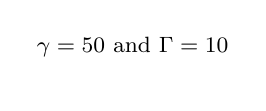
\begin{tikzpicture}[%
font=\footnotesize
]

\begin{axis}[%
width=0.951\figwidth,
height=\figheight,
at={(0\figwidth,0\figheight)},
scale only axis,
xmin=0,
xmax=3,
tick align=outside,
xlabel={Log-Moneyness},
xmajorgrids,
ymin=0,
ymax=5,
ylabel={Remaining Time},
ymajorgrids,
zmin=0,
zmax=4e+24,
zlabel={Optimal Rate},
zmajorgrids,
view={50}{40},
axis background/.style={fill=white},
title={$\gamma = 50$ and $\Gamma = 10$},
axis x line*=bottom,
axis y line*=left,
axis z line*=left
]

\addplot3[%
surf,
shader=flat corner,draw=black,z buffer=sort,colormap={mymap}{[1pt] rgb(0pt)=(0.2081,0.1663,0.5292); rgb(1pt)=(0.211624,0.189781,0.577676); rgb(2pt)=(0.212252,0.213771,0.626971); rgb(3pt)=(0.2081,0.2386,0.677086); rgb(4pt)=(0.195905,0.264457,0.7279); rgb(5pt)=(0.170729,0.291938,0.779248); rgb(6pt)=(0.125271,0.324243,0.830271); rgb(7pt)=(0.0591333,0.359833,0.868333); rgb(8pt)=(0.0116952,0.38751,0.881957); rgb(9pt)=(0.00595714,0.408614,0.882843); rgb(10pt)=(0.0165143,0.4266,0.878633); rgb(11pt)=(0.0328524,0.443043,0.871957); rgb(12pt)=(0.0498143,0.458571,0.864057); rgb(13pt)=(0.0629333,0.47369,0.855438); rgb(14pt)=(0.0722667,0.488667,0.8467); rgb(15pt)=(0.0779429,0.503986,0.838371); rgb(16pt)=(0.0793476,0.520024,0.831181); rgb(17pt)=(0.0749429,0.537543,0.826271); rgb(18pt)=(0.0640571,0.556986,0.823957); rgb(19pt)=(0.0487714,0.577224,0.822829); rgb(20pt)=(0.0343429,0.596581,0.819852); rgb(21pt)=(0.0265,0.6137,0.8135); rgb(22pt)=(0.0238905,0.628662,0.803762); rgb(23pt)=(0.0230905,0.641786,0.791267); rgb(24pt)=(0.0227714,0.653486,0.776757); rgb(25pt)=(0.0266619,0.664195,0.760719); rgb(26pt)=(0.0383714,0.674271,0.743552); rgb(27pt)=(0.0589714,0.683757,0.725386); rgb(28pt)=(0.0843,0.692833,0.706167); rgb(29pt)=(0.113295,0.7015,0.685857); rgb(30pt)=(0.145271,0.709757,0.664629); rgb(31pt)=(0.180133,0.717657,0.642433); rgb(32pt)=(0.217829,0.725043,0.619262); rgb(33pt)=(0.258643,0.731714,0.595429); rgb(34pt)=(0.302171,0.737605,0.571186); rgb(35pt)=(0.348167,0.742433,0.547267); rgb(36pt)=(0.395257,0.7459,0.524443); rgb(37pt)=(0.44201,0.748081,0.503314); rgb(38pt)=(0.487124,0.749062,0.483976); rgb(39pt)=(0.530029,0.749114,0.466114); rgb(40pt)=(0.570857,0.748519,0.44939); rgb(41pt)=(0.609852,0.747314,0.433686); rgb(42pt)=(0.6473,0.7456,0.4188); rgb(43pt)=(0.683419,0.743476,0.404433); rgb(44pt)=(0.71841,0.741133,0.390476); rgb(45pt)=(0.752486,0.7384,0.376814); rgb(46pt)=(0.785843,0.735567,0.363271); rgb(47pt)=(0.818505,0.732733,0.34979); rgb(48pt)=(0.850657,0.7299,0.336029); rgb(49pt)=(0.882433,0.727433,0.3217); rgb(50pt)=(0.913933,0.725786,0.306276); rgb(51pt)=(0.944957,0.726114,0.288643); rgb(52pt)=(0.973895,0.731395,0.266648); rgb(53pt)=(0.993771,0.745457,0.240348); rgb(54pt)=(0.999043,0.765314,0.216414); rgb(55pt)=(0.995533,0.786057,0.196652); rgb(56pt)=(0.988,0.8066,0.179367); rgb(57pt)=(0.978857,0.827143,0.163314); rgb(58pt)=(0.9697,0.848138,0.147452); rgb(59pt)=(0.962586,0.870514,0.1309); rgb(60pt)=(0.958871,0.8949,0.113243); rgb(61pt)=(0.959824,0.921833,0.0948381); rgb(62pt)=(0.9661,0.951443,0.0755333); rgb(63pt)=(0.9763,0.9831,0.0538)},mesh/rows=25]
table[row sep=crcr, point meta=\thisrow{c}] {%
%
x	y	z	c\\
0	0.01	1018.44695884869	1018.44695884869\\
0	0.111836734693878	1901.6047160984	1901.6047160984\\
0	0.213673469387755	4974.49524636308	4974.49524636308\\
0	0.315510204081633	13699.5185741682	13699.5185741682\\
0	0.41734693877551	37930.5334699764	37930.5334699764\\
0	0.519183673469388	105042.591008651	105042.591008651\\
0	0.621020408163265	290860.887898412	290860.887898412\\
0	0.722857142857143	805331.898219974	805331.898219974\\
0	0.82469387755102	2229732.2699316	2229732.2699316\\
0	0.926530612244898	6173427.02689156	6173427.02689156\\
0	1.02836734693878	17092218.5377211	17092218.5377211\\
0	1.13020408163265	47322756.8010587	47322756.8010587\\
0	1.23204081632653	131021164.37262	131021164.37262\\
0	1.33387755102041	362754500.168058	362754500.168058\\
0	1.43571428571429	1004347818.1796	1004347818.1796\\
0	1.53755102040816	2780708498.27908	2780708498.27908\\
0	1.63938775510204	7698866430.79781	7698866430.79781\\
0	1.74122448979592	21315626653.9368	21315626653.9368\\
0	1.8430612244898	59015952979.8295	59015952979.8295\\
0	1.94489795918367	163395745367.797	163395745367.797\\
0	2.04673469387755	452389027940.434	452389027940.434\\
0	2.14857142857143	1252516288797.04	1252516288797.04\\
0	2.25040816326531	3467805266682.45	3467805266682.45\\
0	2.35224489795918	9601211157998.5	9601211157998.5\\
0	2.45408163265306	26582592911424.5	26582592911424.5\\
0	2.55591836734694	73598448598381.6	73598448598381.6\\
0	2.65775510204082	203769875050797	203769875050797\\
0	2.75959183673469	564171701563951	564171701563951\\
0	2.86142857142857	1.56200571240563e+15	1.56200571240563e+15\\
0	2.96326530612245	4.32467959457082e+15	4.32467959457082e+15\\
0	3.06510204081633	1.19736140829434e+16	1.19736140829434e+16\\
0	3.1669387755102	3.31509955991254e+16	3.31509955991254e+16\\
0	3.26877551020408	9.17841932770173e+16	9.17841932770173e+16\\
0	3.37061224489796	2.5412021519304e+17	2.5412021519304e+17\\
0	3.47244897959184	7.03575217737668e+17	7.03575217737668e+17\\
0	3.57428571428571	1.94796815608925e+18	1.94796815608925e+18\\
0	3.67612244897959	5.39328253962592e+18	5.39328253962592e+18\\
0	3.77795918367347	1.49322238463223e+19	1.49322238463223e+19\\
0	3.87979591836735	4.13424120391348e+19	4.13424120391348e+19\\
0	3.98163265306122	1.14463528728471e+20	1.14463528728471e+20\\
0	4.0834693877551	3.16911828864079e+20	3.16911828864079e+20\\
0	4.18530612244898	8.77424524559364e+20	8.77424524559364e+20\\
0	4.28714285714286	2.42929965428473e+21	2.42929965428473e+21\\
0	4.38897959183674	6.7259310004725e+21	6.7259310004725e+21\\
0	4.49081632653061	1.86218887173184e+22	1.86218887173184e+22\\
0	4.59265306122449	5.15578794037332e+22	5.15578794037332e+22\\
0	4.69448979591837	1.42746794858567e+23	1.42746794858567e+23\\
0	4.79632653061224	3.95218881731517e+23	3.95218881731517e+23\\
0	4.89816326530612	1.09423097472617e+24	1.09423097472617e+24\\
0	5	3.02956534061434e+24	3.02956534061434e+24\\
0.125	0.01	1015.03348600578	1015.03348600578\\
0.125	0.111836734693878	1845.63757550218	1845.63757550218\\
0.125	0.213673469387755	4791.58091652791	4791.58091652791\\
0.125	0.315510204081633	13178.1191401992	13178.1191401992\\
0.125	0.41734693877551	36478.400733629	36478.400733629\\
0.125	0.519183673469388	101016.682360629	101016.682360629\\
0.125	0.621020408163265	279710.625242918	279710.625242918\\
0.125	0.722857142857143	774457.513158539	774457.513158539\\
0.125	0.82469387755102	2144248.80432298	2144248.80432298\\
0.125	0.926530612244898	5936749.33662063	5936749.33662063\\
0.125	1.02836734693878	16436934.0552993	16436934.0552993\\
0.125	1.13020408163265	45508488.1008733	45508488.1008733\\
0.125	1.23204081632653	125998050.061343	125998050.061343\\
0.125	1.33387755102041	348847148.849705	348847148.849705\\
0.125	1.43571428571429	965842939.441472	965842939.441472\\
0.125	1.53755102040816	2674101163.89013	2674101163.89013\\
0.125	1.63938775510204	7403705816.60899	7403705816.60899\\
0.125	1.74122448979592	20498424080.69	20498424080.69\\
0.125	1.8430612244898	56753388082.1727	56753388082.1727\\
0.125	1.94489795918367	157131448017.174	157131448017.174\\
0.125	2.04673469387755	435045250825.581	435045250825.581\\
0.125	2.14857142857143	1204497079656.42	1204497079656.42\\
0.125	2.25040816326531	3334855884826.65	3334855884826.65\\
0.125	2.35224489795918	9233118087494.72	9233118087494.72\\
0.125	2.45408163265306	25563464377984	25563464377984\\
0.125	2.55591836734694	70776817193439.9	70776817193439.9\\
0.125	2.65775510204082	195957706611661	195957706611661\\
0.125	2.75959183673469	542542378918826	542542378918826\\
0.125	2.86142857142857	1.50212123852388e+15	1.50212123852388e+15\\
0.125	2.96326530612245	4.15887920077502e+15	4.15887920077502e+15\\
0.125	3.06510204081633	1.15145673751583e+16	1.15145673751583e+16\\
0.125	3.1669387755102	3.18800463866209e+16	3.18800463866209e+16\\
0.125	3.26877551020408	8.82653533128656e+16	8.82653533128656e+16\\
0.125	3.37061224489796	2.44377705758761e+17	2.44377705758761e+17\\
0.125	3.47244897959184	6.76601416415699e+17	6.76601416415699e+17\\
0.125	3.57428571428571	1.87328658019094e+18	1.87328658019094e+18\\
0.125	3.67612244897959	5.18651384165513e+18	5.18651384165513e+18\\
0.125	3.77795918367347	1.43597493913277e+19	1.43597493913277e+19\\
0.125	3.87979591836735	3.97574187358043e+19	3.97574187358043e+19\\
0.125	3.98163265306122	1.10075204062305e+20	1.10075204062305e+20\\
0.125	4.0834693877551	3.04762002530238e+20	3.04762002530238e+20\\
0.125	4.18530612244898	8.43785655247637e+20	8.43785655247637e+20\\
0.125	4.28714285714286	2.33616469930818e+21	2.33616469930818e+21\\
0.125	4.38897959183674	6.46807097080999e+21	6.46807097080999e+21\\
0.125	4.49081632653061	1.79079591844786e+22	1.79079591844786e+22\\
0.125	4.59265306122449	4.95812435578113e+22	4.95812435578113e+22\\
0.125	4.69448979591837	1.3727414092331e+23	1.3727414092331e+23\\
0.125	4.79632653061224	3.80066904620114e+23	3.80066904620114e+23\\
0.125	4.89816326530612	1.05228013823981e+24	1.05228013823981e+24\\
0.125	5	2.91341728488811e+24	2.91341728488811e+24\\
0.25	0.01	1015.0208433828	1015.0208433828\\
0.25	0.111836734693878	1832.53995993597	1832.53995993597\\
0.25	0.213673469387755	4733.93014033886	4733.93014033886\\
0.25	0.315510204081633	13001.5771466767	13001.5771466767\\
0.25	0.41734693877551	35977.4349248078	35977.4349248078\\
0.25	0.519183673469388	99620.8154974655	99620.8154974655\\
0.25	0.621020408163265	275839.227403761	275839.227403761\\
0.25	0.722857142857143	763733.589394427	763733.589394427\\
0.25	0.82469387755102	2114553.43774316	2114553.43774316\\
0.25	0.926530612244898	5854528.95443012	5854528.95443012\\
0.25	1.02836734693878	16209289.6826907	16209289.6826907\\
0.25	1.13020408163265	44878212.9429415	44878212.9429415\\
0.25	1.23204081632653	124253023.097728	124253023.097728\\
0.25	1.33387755102041	344015741.353055	344015741.353055\\
0.25	1.43571428571429	952466360.493925	952466360.493925\\
0.25	1.53755102040816	2637065818.46799	2637065818.46799\\
0.25	1.63938775510204	7301167135.55654	7301167135.55654\\
0.25	1.74122448979592	20214528227.9419	20214528227.9419\\
0.25	1.8430612244898	55967373924.7894	55967373924.7894\\
0.25	1.94489795918367	154955233575.163	154955233575.163\\
0.25	2.04673469387755	429020029459.06	429020029459.06\\
0.25	2.14857142857143	1187815225235.69	1187815225235.69\\
0.25	2.25040816326531	3288669321716.2	3288669321716.2\\
0.25	2.35224489795918	9105242699176.55	9105242699176.55\\
0.25	2.45408163265306	25209419525191.8	25209419525191.8\\
0.25	2.55591836734694	69796583550070.1	69796583550070.1\\
0.25	2.65775510204082	193243762332276	193243762332276\\
0.25	2.75959183673469	535028360715408	535028360715408\\
0.25	2.86142857142857	1.48131739578533e+15	1.48131739578533e+15\\
0.25	2.96326530612245	4.10128020900079e+15	4.10128020900079e+15\\
0.25	3.06510204081633	1.13550947289217e+16	1.13550947289217e+16\\
0.25	3.1669387755102	3.14385191286901e+16	3.14385191286901e+16\\
0.25	3.26877551020408	8.70429096894848e+16	8.70429096894848e+16\\
0.25	3.37061224489796	2.4099316180253e+17	2.4099316180253e+17\\
0.25	3.47244897959184	6.67230728416229e+17	6.67230728416229e+17\\
0.25	3.57428571428571	1.84734223001589e+18	1.84734223001589e+18\\
0.25	3.67612244897959	5.11468247708044e+18	5.11468247708044e+18\\
0.25	3.77795918367347	1.41608719902035e+19	1.41608719902035e+19\\
0.25	3.87979591836735	3.92067926839088e+19	3.92067926839088e+19\\
0.25	3.98163265306122	1.08550701794507e+20	1.08550701794507e+20\\
0.25	4.0834693877551	3.00541157627363e+20	3.00541157627363e+20\\
0.25	4.18530612244898	8.32099525242737e+20	8.32099525242737e+20\\
0.25	4.28714285714286	2.30380965247925e+21	2.30380965247925e+21\\
0.25	4.38897959183674	6.37849049764871e+21	6.37849049764871e+21\\
0.25	4.49081632653061	1.76599403448158e+22	1.76599403448158e+22\\
0.25	4.59265306122449	4.88945610403307e+22	4.88945610403307e+22\\
0.25	4.69448979591837	1.3537294309312e+23	1.3537294309312e+23\\
0.25	4.79632653061224	3.74803113715998e+23	3.74803113715998e+23\\
0.25	4.89816326530612	1.03770643410314e+24	1.03770643410314e+24\\
0.25	5	2.87306749589869e+24	2.87306749589869e+24\\
0.375	0.01	1015.02084305779	1015.02084305779\\
0.375	0.111836734693878	1830.27868866952	1830.27868866952\\
0.375	0.213673469387755	4717.5698250153	4717.5698250153\\
0.375	0.315510204081633	12943.9656035387	12943.9656035387\\
0.375	0.41734693877551	35806.7183826767	35806.7183826767\\
0.375	0.519183673469388	99138.7459606863	99138.7459606863\\
0.375	0.621020408163265	274496.749907866	274496.749907866\\
0.375	0.722857142857143	760010.213740783	760010.213740783\\
0.375	0.82469387755102	2104239.12449772	2104239.12449772\\
0.375	0.926530612244898	5825967.25900041	5825967.25900041\\
0.375	1.02836734693878	16130207.5784901	16130207.5784901\\
0.375	1.13020408163265	44659256.9213517	44659256.9213517\\
0.375	1.23204081632653	123646802.61926	123646802.61926\\
0.375	1.33387755102041	342337313.38954	342337313.38954\\
0.375	1.43571428571429	947819343.237326	947819343.237326\\
0.375	1.53755102040816	2624199754.95419	2624199754.95419\\
0.375	1.63938775510204	7265545238.90712	7265545238.90712\\
0.375	1.74122448979592	20115902920.8805	20115902920.8805\\
0.375	1.8430612244898	55694312915.5913	55694312915.5913\\
0.375	1.94489795918367	154199217532.31	154199217532.31\\
0.375	2.04673469387755	426926869920.26	426926869920.26\\
0.375	2.14857142857143	1182019955555.11	1182019955555.11\\
0.375	2.25040816326531	3272624127807.62	3272624127807.62\\
0.375	2.35224489795918	9060818839430.84	9060818839430.84\\
0.375	2.45408163265306	25086424482196.2	25086424482196.2\\
0.375	2.55591836734694	69456050766833.4	69456050766833.4\\
0.375	2.65775510204082	192300939161244	192300939161244\\
0.375	2.75959183673469	532417993738748	532417993738748\\
0.375	2.86142857142857	1.47409014897788e+15	1.47409014897788e+15\\
0.375	2.96326530612245	4.08127034185072e+15	4.08127034185072e+15\\
0.375	3.06510204081633	1.12996939941699e+16	1.12996939941699e+16\\
0.375	3.1669387755102	3.12851327324661e+16	3.12851327324661e+16\\
0.375	3.26877551020408	8.66182332541944e+16	8.66182332541944e+16\\
0.375	3.37061224489796	2.39817372559591e+17	2.39817372559591e+17\\
0.375	3.47244897959184	6.63975355080339e+17	6.63975355080339e+17\\
0.375	3.57428571428571	1.83832917293977e+18	1.83832917293977e+18\\
0.375	3.67612244897959	5.08972828919614e+18	5.08972828919614e+18\\
0.375	3.77795918367347	1.40917820590403e+19	1.40917820590403e+19\\
0.375	3.87979591836735	3.90155054093969e+19	3.90155054093969e+19\\
0.375	3.98163265306122	1.08021090304482e+20	1.08021090304482e+20\\
0.375	4.0834693877551	2.99074837763315e+20	2.99074837763315e+20\\
0.375	4.18530612244898	8.28039768262188e+20	8.28039768262188e+20\\
0.375	4.28714285714286	2.29256952190115e+21	2.29256952190115e+21\\
0.375	4.38897959183674	6.34737027640666e+21	6.34737027640666e+21\\
0.375	4.49081632653061	1.75737786971886e+22	1.75737786971886e+22\\
0.375	4.59265306122449	4.86560078030612e+22	4.86560078030612e+22\\
0.375	4.69448979591837	1.34712467712496e+23	1.34712467712496e+23\\
0.375	4.79632653061224	3.72974474820113e+23	3.72974474820113e+23\\
0.375	4.89816326530612	1.03264353500101e+24	1.03264353500101e+24\\
0.375	5	2.85904999502628e+24	2.85904999502628e+24\\
0.5	0.01	1015.02084305779	1015.02084305779\\
0.5	0.111836734693878	1830.00826132611	1830.00826132611\\
0.5	0.213673469387755	4713.55358515722	4713.55358515722\\
0.5	0.315510204081633	12926.2714909695	12926.2714909695\\
0.5	0.41734693877551	35749.9045996251	35749.9045996251\\
0.5	0.519183673469388	98973.6936672223	98973.6936672223\\
0.5	0.621020408163265	274032.621744694	274032.621744694\\
0.5	0.722857142857143	758718.769866015	758718.769866015\\
0.5	0.82469387755102	2100657.8072449	2100657.8072449\\
0.5	0.926530612244898	5816046.64276431	5816046.64276431\\
0.5	1.02836734693878	16102736.0469083	16102736.0469083\\
0.5	1.13020408163265	44583193.1195096	44583193.1195096\\
0.5	1.23204081632653	123436203.187297	123436203.187297\\
0.5	1.33387755102041	341754229.40217	341754229.40217\\
0.5	1.43571428571429	946204972.410103	946204972.410103\\
0.5	1.53755102040816	2619730090.60732	2619730090.60732\\
0.5	1.63938775510204	7253170206.99017	7253170206.99017\\
0.5	1.74122448979592	20081640528.838	20081640528.838\\
0.5	1.8430612244898	55599451628.9919	55599451628.9919\\
0.5	1.94489795918367	153936577856.397	153936577856.397\\
0.5	2.04673469387755	426199707118.271	426199707118.271\\
0.5	2.14857142857143	1180006681139.84	1180006681139.84\\
0.5	2.25040816326531	3267050033737.86	3267050033737.86\\
0.5	2.35224489795918	9045386007980.17	9045386007980.17\\
0.5	2.45408163265306	25043696052502.3	25043696052502.3\\
0.5	2.55591836734694	69337749811502.2	69337749811502.2\\
0.5	2.65775510204082	191973402761415	191973402761415\\
0.5	2.75959183673469	531511153274889	531511153274889\\
0.5	2.86142857142857	1.47157940627161e+15	1.47157940627161e+15\\
0.5	2.96326530612245	4.0743189218509e+15	4.0743189218509e+15\\
0.5	3.06510204081633	1.12804478006459e+16	1.12804478006459e+16\\
0.5	3.1669387755102	3.12318463585781e+16	3.12318463585781e+16\\
0.5	3.26877551020408	8.64707008271414e+16	8.64707008271414e+16\\
0.5	3.37061224489796	2.39408903837777e+17	2.39408903837777e+17\\
0.5	3.47244897959184	6.62844439660362e+17	6.62844439660362e+17\\
0.5	3.57428571428571	1.83519804044703e+18	1.83519804044703e+18\\
0.5	3.67612244897959	5.0810592141142e+18	5.0810592141142e+18\\
0.5	3.77795918367347	1.40677802440799e+19	1.40677802440799e+19\\
0.5	3.87979591836735	3.8949052285274e+19	3.8949052285274e+19\\
0.5	3.98163265306122	1.07837103480614e+20	1.07837103480614e+20\\
0.5	4.0834693877551	2.98565438817759e+20	2.98565438817759e+20\\
0.5	4.18530612244898	8.26629410279597e+20	8.26629410279597e+20\\
0.5	4.28714285714286	2.28866470494695e+21	2.28866470494695e+21\\
0.5	4.38897959183674	6.33655912375323e+21	6.33655912375323e+21\\
0.5	4.49081632653061	1.75438461745974e+22	1.75438461745974e+22\\
0.5	4.59265306122449	4.85731345019995e+22	4.85731345019995e+22\\
0.5	4.69448979591837	1.3448301882432e+23	1.3448301882432e+23\\
0.5	4.79632653061224	3.72339206384913e+23	3.72339206384913e+23\\
0.5	4.89816326530612	1.0308846858387e+24	1.0308846858387e+24\\
0.5	5	2.85418032072113e+24	2.85418032072113e+24\\
0.625	0.01	1015.02084305779	1015.02084305779\\
0.625	0.111836734693878	1829.98687743829	1829.98687743829\\
0.625	0.213673469387755	4712.7283267327	4712.7283267327\\
0.625	0.315510204081633	12921.282155675	12921.282155675\\
0.625	0.41734693877551	35731.7145958222	35731.7145958222\\
0.625	0.519183673469388	98918.0849303821	98918.0849303821\\
0.625	0.621020408163265	273873.159328346	273873.159328346\\
0.625	0.722857142857143	758271.866108539	758271.866108539\\
0.625	0.82469387755102	2099415.33218101	2099415.33218101\\
0.625	0.926530612244898	5812601.81196583	5812601.81196583\\
0.625	1.02836734693878	16093193.9455951	16093193.9455951\\
0.625	1.13020408163265	44556769.99544	44556769.99544\\
0.625	1.23204081632653	123363042.355953	123363042.355953\\
0.625	1.33387755102041	341551667.506248	341551667.506248\\
0.625	1.43571428571429	945644141.800559	945644141.800559\\
0.625	1.53755102040816	2618177332.08489	2618177332.08489\\
0.625	1.63938775510204	7248871126.81573	7248871126.81573\\
0.625	1.74122448979592	20069737788.2876	20069737788.2876\\
0.625	1.8430612244898	55566496856.1918	55566496856.1918\\
0.625	1.94489795918367	153845336936.911	153845336936.911\\
0.625	2.04673469387755	425947091046.941	425947091046.941\\
0.625	2.14857142857143	1179307270398.98	1179307270398.98\\
0.625	2.25040816326531	3265113595645.04	3265113595645.04\\
0.625	2.35224489795918	9040024648387.8	9040024648387.8\\
0.625	2.45408163265306	25028852212785.7	25028852212785.7\\
0.625	2.55591836734694	69296652106021.1	69296652106021.1\\
0.625	2.65775510204082	191859616744593	191859616744593\\
0.625	2.75959183673469	531196117253427	531196117253427\\
0.625	2.86142857142857	1.47070717524021e+15	1.47070717524021e+15\\
0.625	2.96326530612245	4.07190400126946e+15	4.07190400126946e+15\\
0.625	3.06510204081633	1.12737616805644e+16	1.12737616805644e+16\\
0.625	3.1669387755102	3.12133346931896e+16	3.12133346931896e+16\\
0.625	3.26877551020408	8.64194481198492e+16	8.64194481198492e+16\\
0.625	3.37061224489796	2.39267001964031e+17	2.39267001964031e+17\\
0.625	3.47244897959184	6.62451560087043e+17	6.62451560087043e+17\\
0.625	3.57428571428571	1.83411028624719e+18	1.83411028624719e+18\\
0.625	3.67612244897959	5.07804758083107e+18	5.07804758083107e+18\\
0.625	3.77795918367347	1.40594420229473e+19	1.40594420229473e+19\\
0.625	3.87979591836735	3.89259664960187e+19	3.89259664960187e+19\\
0.625	3.98163265306122	1.07773186530166e+20	1.07773186530166e+20\\
0.625	4.0834693877551	2.9838847382387e+20	2.9838847382387e+20\\
0.625	4.18530612244898	8.26139452469618e+20	8.26139452469618e+20\\
0.625	4.28714285714286	2.28730817306862e+21	2.28730817306862e+21\\
0.625	4.38897959183674	6.3328033335618e+21	6.3328033335618e+21\\
0.625	4.49081632653061	1.75334476279894e+22	1.75334476279894e+22\\
0.625	4.59265306122449	4.85443443497155e+22	4.85443443497155e+22\\
0.625	4.69448979591837	1.34403308370563e+23	1.34403308370563e+23\\
0.625	4.79632653061224	3.72118514379691e+23	3.72118514379691e+23\\
0.625	4.89816326530612	1.03027366232957e+24	1.03027366232957e+24\\
0.625	5	2.85248859777753e+24	2.85248859777753e+24\\
0.75	0.01	1015.02084305779	1015.02084305779\\
0.75	0.111836734693878	1829.98579703967	1829.98579703967\\
0.75	0.213673469387755	4712.58989693264	4712.58989693264\\
0.75	0.315510204081633	12920.0190819042	12920.0190819042\\
0.75	0.41734693877551	35726.2044418754	35726.2044418754\\
0.75	0.519183673469388	98899.8330824298	98899.8330824298\\
0.75	0.621020408163265	273818.990108056	273818.990108056\\
0.75	0.722857142857143	758117.923586667	758117.923586667\\
0.75	0.82469387755102	2098985.03831002	2098985.03831002\\
0.75	0.926530612244898	5811406.4159134	5811406.4159134\\
0.75	1.02836734693878	16089880.3347024	16089880.3347024\\
0.75	1.13020408163265	44547591.8866108	44547591.8866108\\
0.75	1.23204081632653	123337627.5426	123337627.5426\\
0.75	1.33387755102041	341481298.767901	341481298.767901\\
0.75	1.43571428571429	945449310.605287	945449310.605287\\
0.75	1.53755102040816	2617637905.47626	2617637905.47626\\
0.75	1.63938775510204	7247377629.09845	7247377629.09845\\
0.75	1.74122448979592	20065602781.8961	20065602781.8961\\
0.75	1.8430612244898	55555048382.014	55555048382.014\\
0.75	1.94489795918367	153813639878.198	153813639878.198\\
0.75	2.04673469387755	425859332323.737	425859332323.737\\
0.75	2.14857142857143	1179064295382.79	1179064295382.79\\
0.75	2.25040816326531	3264440877811.95	3264440877811.95\\
0.75	2.35224489795918	9038162114169.12	9038162114169.12\\
0.75	2.45408163265306	25023695468691.2	25023695468691.2\\
0.75	2.55591836734694	69282374779257.2	69282374779257.2\\
0.75	2.65775510204082	191820087526976	191820087526976\\
0.75	2.75959183673469	531086673863137	531086673863137\\
0.75	2.86142857142857	1.47040416252202e+15	1.47040416252202e+15\\
0.75	2.96326530612245	4.07106505880666e+15	4.07106505880666e+15\\
0.75	3.06510204081633	1.12714389250706e+16	1.12714389250706e+16\\
0.75	3.1669387755102	3.12069037478943e+16	3.12069037478943e+16\\
0.75	3.26877551020408	8.64016429494377e+16	8.64016429494377e+16\\
0.75	3.37061224489796	2.39217705308746e+17	2.39217705308746e+17\\
0.75	3.47244897959184	6.62315073877353e+17	6.62315073877353e+17\\
0.75	3.57428571428571	1.83373240086476e+18	1.83373240086476e+18\\
0.75	3.67612244897959	5.07700134060956e+18	5.07700134060956e+18\\
0.75	3.77795918367347	1.40565453282035e+19	1.40565453282035e+19\\
0.75	3.87979591836735	3.89179465018854e+19	3.89179465018854e+19\\
0.75	3.98163265306122	1.07750981806649e+20	1.07750981806649e+20\\
0.75	4.0834693877551	2.98326996254402e+20	2.98326996254402e+20\\
0.75	4.18530612244898	8.25969241318602e+20	8.25969241318602e+20\\
0.75	4.28714285714286	2.28683691442615e+21	2.28683691442615e+21\\
0.75	4.38897959183674	6.3314985735224e+21	6.3314985735224e+21\\
0.75	4.49081632653061	1.75298351769764e+22	1.75298351769764e+22\\
0.75	4.59265306122449	4.85343426621042e+22	4.85343426621042e+22\\
0.75	4.69448979591837	1.34375616990192e+23	1.34375616990192e+23\\
0.75	4.79632653061224	3.72041846063638e+23	3.72041846063638e+23\\
0.75	4.89816326530612	1.03006139300216e+24	1.03006139300216e+24\\
0.75	5	2.85190089389045e+24	2.85190089389045e+24\\
0.875	0.01	1015.02084305779	1015.02084305779\\
0.875	0.111836734693878	1829.98576303668	1829.98576303668\\
0.875	0.213673469387755	4712.57128904114	4712.57128904114\\
0.875	0.315510204081633	12919.7372454903	12919.7372454903\\
0.875	0.41734693877551	35724.6507382	35724.6507382\\
0.875	0.519183673469388	98894.0654053764	98894.0654053764\\
0.875	0.621020408163265	273800.923849461	273800.923849461\\
0.875	0.722857142857143	758065.328856289	758065.328856289\\
0.875	0.82469387755102	2098836.52844257	2098836.52844257\\
0.875	0.926530612244898	5810992.16390582	5810992.16390582\\
0.875	1.02836734693878	16088730.2434263	16088730.2434263\\
0.875	1.13020408163265	44544404.4799332	44544404.4799332\\
0.875	1.23204081632653	123328799.506912	123328799.506912\\
0.875	1.33387755102041	341456853.743185	341456853.743185\\
0.875	1.43571428571429	945381627.352872	945381627.352872\\
0.875	1.53755102040816	2617450509.88969	2617450509.88969\\
0.875	1.63938775510204	7246858789.55801	7246858789.55801\\
0.875	1.74122448979592	20064166283.2522	20064166283.2522\\
0.875	1.8430612244898	55551071187.5031	55551071187.5031\\
0.875	1.94489795918367	153802628333.335	153802628333.335\\
0.875	2.04673469387755	425828844978.592	425828844978.592\\
0.875	2.14857142857143	1178979885958.32	1178979885958.32\\
0.875	2.25040816326531	3264207175901.42	3264207175901.42\\
0.875	2.35224489795918	9037515070512.88	9037515070512.88\\
0.875	2.45408163265306	25021904017816.1	25021904017816.1\\
0.875	2.55591836734694	69277414841540	69277414841540\\
0.875	2.65775510204082	191806355092281	191806355092281\\
0.875	2.75959183673469	531048653272277	531048653272277\\
0.875	2.86142857142857	1.47029889602257e+15	1.47029889602257e+15\\
0.875	2.96326530612245	4.07077361052413e+15	4.07077361052413e+15\\
0.875	3.06510204081633	1.12706320007231e+16	1.12706320007231e+16\\
0.875	3.1669387755102	3.12046696400211e+16	3.12046696400211e+16\\
0.875	3.26877551020408	8.63954574402205e+16	8.63954574402205e+16\\
0.875	3.37061224489796	2.39200579670036e+17	2.39200579670036e+17\\
0.875	3.47244897959184	6.62267658621644e+17	6.62267658621644e+17\\
0.875	3.57428571428571	1.83360112363113e+18	1.83360112363113e+18\\
0.875	3.67612244897959	5.07663787716702e+18	5.07663787716702e+18\\
0.875	3.77795918367347	1.40555390175858e+19	1.40555390175858e+19\\
0.875	3.87979591836735	3.89151603590693e+19	3.89151603590693e+19\\
0.875	3.98163265306122	1.07743267894409e+20	1.07743267894409e+20\\
0.875	4.0834693877551	2.98305638970882e+20	2.98305638970882e+20\\
0.875	4.18530612244898	8.25910110031502e+20	8.25910110031502e+20\\
0.875	4.28714285714286	2.2866731993586e+21	2.2866731993586e+21\\
0.875	4.38897959183674	6.33104530039647e+21	6.33104530039647e+21\\
0.875	4.49081632653061	1.75285802129113e+22	1.75285802129113e+22\\
0.875	4.59265306122449	4.85308680797509e+22	4.85308680797509e+22\\
0.875	4.69448979591837	1.34365997015512e+23	1.34365997015512e+23\\
0.875	4.79632653061224	3.72015211520712e+23	3.72015211520712e+23\\
0.875	4.89816326530612	1.02998765072107e+24	1.02998765072107e+24\\
0.875	5	2.85169672579059e+24	2.85169672579059e+24\\
1	0.01	1015.02084305779	1015.02084305779\\
1	0.111836734693878	1829.98576238255	1829.98576238255\\
1	0.213673469387755	4712.56931192886	4712.56931192886\\
1	0.315510204081633	12919.6826033596	12919.6826033596\\
1	0.41734693877551	35724.2487840567	35724.2487840567\\
1	0.519183673469388	98892.3319393497	98892.3319393497\\
1	0.621020408163265	273795.058538806	273795.058538806\\
1	0.722857142857143	758047.596374677	758047.596374677\\
1	0.82469387755102	2098785.58088847	2098785.58088847\\
1	0.926530612244898	5810848.97942907	5810848.97942907\\
1	1.02836734693878	16088331.4885184	16088331.4885184\\
1	1.13020408163265	44543298.0038374	44543298.0038374\\
1	1.23204081632653	123325733.505082	123325733.505082\\
1	1.33387755102041	341448362.420517	341448362.420517\\
1	1.43571428571429	945358115.093046	945358115.093046\\
1	1.53755102040816	2617385409.61146	2617385409.61146\\
1	1.63938775510204	7246678545.77475	7246678545.77475\\
1	1.74122448979592	20063667245.0472	20063667245.0472\\
1	1.8430612244898	55549689512.5387	55549689512.5387\\
1	1.94489795918367	153798802927.804	153798802927.804\\
1	2.04673469387755	425818253687.667	425818253687.667\\
1	2.14857142857143	1178950562158.16	1178950562158.16\\
1	2.25040816326531	3264125987950.15	3264125987950.15\\
1	2.35224489795918	9037290287801.26	9037290287801.26\\
1	2.45408163265306	25021281668485.5	25021281668485.5\\
1	2.55591836734694	69275691761123.2	69275691761123.2\\
1	2.65775510204082	191801584449855	191801584449855\\
1	2.75959183673469	531035444933926	531035444933926\\
1	2.86142857142857	1.47026232648195e+15	1.47026232648195e+15\\
1	2.96326530612245	4.0706723615051e+15	4.0706723615051e+15\\
1	3.06510204081633	1.12703516755212e+16	1.12703516755212e+16\\
1	3.1669387755102	3.12038935118222e+16	3.12038935118222e+16\\
1	3.26877551020408	8.63933085967445e+16	8.63933085967445e+16\\
1	3.37061224489796	2.39194630229865e+17	2.39194630229865e+17\\
1	3.47244897959184	6.62251186580408e+17	6.62251186580408e+17\\
1	3.57428571428571	1.83355551797165e+18	1.83355551797165e+18\\
1	3.67612244897959	5.07651161010964e+18	5.07651161010964e+18\\
1	3.77795918367347	1.40551894256719e+19	1.40551894256719e+19\\
1	3.87979591836735	3.89141924541478e+19	3.89141924541478e+19\\
1	3.98163265306122	1.07740588084323e+20	1.07740588084323e+20\\
1	4.0834693877551	2.98298219458964e+20	2.98298219458964e+20\\
1	4.18530612244898	8.25889567845556e+20	8.25889567845556e+20\\
1	4.28714285714286	2.28661632480834e+21	2.28661632480834e+21\\
1	4.38897959183674	6.33088783349031e+21	6.33088783349031e+21\\
1	4.49081632653061	1.75281442388873e+22	1.75281442388873e+22\\
1	4.59265306122449	4.85296610112042e+22	4.85296610112042e+22\\
1	4.69448979591837	1.34362655040081e+23	1.34362655040081e+23\\
1	4.79632653061224	3.72005958690946e+23	3.72005958690946e+23\\
1	4.89816326530612	1.02996203268155e+24	1.02996203268155e+24\\
1	5	2.85162579787278e+24	2.85162579787278e+24\\
1.125	0.01	1015.02084305779	1015.02084305779\\
1.125	0.111836734693878	1829.98576237496	1829.98576237496\\
1.125	0.213673469387755	4712.56914759071	4712.56914759071\\
1.125	0.315510204081633	12919.6734981259	12919.6734981259\\
1.125	0.41734693877551	35724.1545100937	35724.1545100937\\
1.125	0.519183673469388	98891.8421207244	98891.8421207244\\
1.125	0.621020408163265	273793.222142061	273793.222142061\\
1.125	0.722857142857143	758041.733850011	758041.733850011\\
1.125	0.82469387755102	2098768.27248319	2098768.27248319\\
1.125	0.926530612244898	5810799.7109223	5810799.7109223\\
1.125	1.02836734693878	16088193.5051024	16088193.5051024\\
1.125	1.13020408163265	44542914.2153608	44542914.2153608\\
1.125	1.23204081632653	123324669.022922	123324669.022922\\
1.125	1.33387755102041	341445413.218091	341445413.218091\\
1.125	1.43571428571429	945349947.647913	945349947.647913\\
1.125	1.53755102040816	2617362794.52245	2617362794.52245\\
1.125	1.63938775510204	7246615929.88851	7246615929.88851\\
1.125	1.74122448979592	20063493880.1101	20063493880.1101\\
1.125	1.8430612244898	55549209519.9398	55549209519.9398\\
1.125	1.94489795918367	153797473984.164	153797473984.164\\
1.125	2.04673469387755	425814574278.091	425814574278.091\\
1.125	2.14857142857143	1178940375082.23	1178940375082.23\\
1.125	2.25040816326531	3264097783288.45	3264097783288.45\\
1.125	2.35224489795918	9037212198376.13	9037212198376.13\\
1.125	2.45408163265306	25021065464572.9	25021065464572.9\\
1.125	2.55591836734694	69275093163663	69275093163663\\
1.125	2.65775510204082	191799927130548	191799927130548\\
1.125	2.75959183673469	531030856362364	531030856362364\\
1.125	2.86142857142857	1.47024962223788e+15	1.47024962223788e+15\\
1.125	2.96326530612245	4.0706371876356e+15	4.0706371876356e+15\\
1.125	3.06510204081633	1.12702542906561e+16	1.12702542906561e+16\\
1.125	3.1669387755102	3.12036238851903e+16	3.12036238851903e+16\\
1.125	3.26877551020408	8.63925620893638e+16	8.63925620893638e+16\\
1.125	3.37061224489796	2.39192563396683e+17	2.39192563396683e+17\\
1.125	3.47244897959184	6.62245464199743e+17	6.62245464199743e+17\\
1.125	3.57428571428571	1.83353967458344e+18	1.83353967458344e+18\\
1.125	3.67612244897959	5.07646774498343e+18	5.07646774498343e+18\\
1.125	3.77795918367347	1.40550679775781e+19	1.40550679775781e+19\\
1.125	3.87979591836735	3.89138562043577e+19	3.89138562043577e+19\\
1.125	3.98163265306122	1.0773965711935e+20	1.0773965711935e+20\\
1.125	4.0834693877551	2.98295641923434e+20	2.98295641923434e+20\\
1.125	4.18530612244898	8.25882431498215e+20	8.25882431498215e+20\\
1.125	4.28714285714286	2.28659656661189e+21	2.28659656661189e+21\\
1.125	4.38897959183674	6.33083312954887e+21	6.33083312954887e+21\\
1.125	4.49081632653061	1.75279927816824e+22	1.75279927816824e+22\\
1.125	4.59265306122449	4.85292416760645e+22	4.85292416760645e+22\\
1.125	4.69448979591837	1.34361494039127e+23	1.34361494039127e+23\\
1.125	4.79632653061224	3.72002744261514e+23	3.72002744261514e+23\\
1.125	4.89816326530612	1.02995313298466e+24	1.02995313298466e+24\\
1.125	5	2.85160115754195e+24	2.85160115754195e+24\\
1.25	0.01	1015.02084305779	1015.02084305779\\
1.25	0.111836734693878	1829.98576237491	1829.98576237491\\
1.25	0.213673469387755	4712.56913698941	4712.56913698941\\
1.25	0.315510204081633	12919.6722048137	12919.6722048137\\
1.25	0.41734693877551	35724.134654799	35724.134654799\\
1.25	0.519183673469388	98891.7133104196	98891.7133104196\\
1.25	0.621020408163265	273792.672786472	273792.672786472\\
1.25	0.722857142857143	758039.846925535	758039.846925535\\
1.25	0.82469387755102	2098762.47712578	2098762.47712578\\
1.25	0.926530612244898	5810782.88098436	5810782.88098436\\
1.25	1.02836734693878	16088145.9201028	16088145.9201028\\
1.25	1.13020408163265	44542781.29585	44542781.29585\\
1.25	1.23204081632653	123324299.68127	123324299.68127\\
1.25	1.33387755102041	341444389.168265	341444389.168265\\
1.25	1.43571428571429	945347110.818222	945347110.818222\\
1.25	1.53755102040816	2617354938.6159	2617354938.6159\\
1.25	1.63938775510204	7246594177.74371	7246594177.74371\\
1.25	1.74122448979592	20063433653.8064	20063433653.8064\\
1.25	1.8430612244898	55549042771.3201	55549042771.3201\\
1.25	1.94489795918367	153797012310.295	153797012310.295\\
1.25	2.04673469387755	425813296053.284	425813296053.284\\
1.25	2.14857142857143	1178936836096.68	1178936836096.68\\
1.25	2.25040816326531	3264087985000.68	3264087985000.68\\
1.25	2.35224489795918	9037185070141.11	9037185070141.11\\
1.25	2.45408163265306	25020990355419.1	25020990355419.1\\
1.25	2.55591836734694	69274885211140.7	69274885211140.7\\
1.25	2.65775510204082	191799351378471	191799351378471\\
1.25	2.75959183673469	531029262294403	531029262294403\\
1.25	2.86142857142857	1.47024520878847e+15	1.47024520878847e+15\\
1.25	2.96326530612245	4.07062496824713e+15	4.07062496824713e+15\\
1.25	3.06510204081633	1.12702204591921e+16	1.12702204591921e+16\\
1.25	3.1669387755102	3.12035302170041e+16	3.12035302170041e+16\\
1.25	3.26877551020408	8.63923027529925e+16	8.63923027529925e+16\\
1.25	3.37061224489796	2.39191845379646e+17	2.39191845379646e+17\\
1.25	3.47244897959184	6.62243476246945e+17	6.62243476246945e+17\\
1.25	3.57428571428571	1.83353417059659e+18	1.83353417059659e+18\\
1.25	3.67612244897959	5.07645250625579e+18	5.07645250625579e+18\\
1.25	3.77795918367347	1.4055025786558e+19	1.4055025786558e+19\\
1.25	3.87979591836735	3.89137393913125e+19	3.89137393913125e+19\\
1.25	3.98163265306122	1.07739333702483e+20	1.07739333702483e+20\\
1.25	4.0834693877551	2.98294746488602e+20	2.98294746488602e+20\\
1.25	4.18530612244898	8.25879952333948e+20	8.25879952333948e+20\\
1.25	4.28714285714286	2.28658970262219e+21	2.28658970262219e+21\\
1.25	4.38897959183674	6.33081412542107e+21	6.33081412542107e+21\\
1.25	4.49081632653061	1.75279401655088e+22	1.75279401655088e+22\\
1.25	4.59265306122449	4.85290959992014e+22	4.85290959992014e+22\\
1.25	4.69448979591837	1.34361090707851e+23	1.34361090707851e+23\\
1.25	4.79632653061224	3.72001627569991e+23	3.72001627569991e+23\\
1.25	4.89816326530612	1.02995004123346e+24	1.02995004123346e+24\\
1.25	5	2.85159259750069e+24	2.85159259750069e+24\\
1.375	0.01	1015.02084305779	1015.02084305779\\
1.375	0.111836734693878	1829.98576237491	1829.98576237491\\
1.375	0.213673469387755	4712.56913646196	4712.56913646196\\
1.375	0.315510204081633	12919.6720492089	12919.6720492089\\
1.375	0.41734693877551	35724.130927435	35724.130927435\\
1.375	0.519183673469388	98891.68205175	98891.68205175\\
1.375	0.621020408163265	273792.517116166	273792.517116166\\
1.375	0.722857142857143	758039.260098284	758039.260098284\\
1.375	0.82469387755102	2098760.57538867	2098760.57538867\\
1.375	0.926530612244898	5810777.19438176	5810777.19438176\\
1.375	1.02836734693878	16088129.5998122	16088129.5998122\\
1.375	1.13020408163265	44542735.3801994	44542735.3801994\\
1.375	1.23204081632653	123324171.679714	123324171.679714\\
1.375	1.33387755102041	341444033.764456	341444033.764456\\
1.375	1.43571428571429	945346125.693978	945346125.693978\\
1.375	1.53755102040816	2617352209.9002	2617352209.9002\\
1.375	1.63938775510204	7246586621.50961	7246586621.50961\\
1.375	1.74122448979592	20063412731.6896	20063412731.6896\\
1.375	1.8430612244898	55548984843.4134	55548984843.4134\\
1.375	1.94489795918367	153796851925.49	153796851925.49\\
1.375	2.04673469387755	425812851999.018	425812851999.018\\
1.375	2.14857142857143	1178935606655.03	1178935606655.03\\
1.375	2.25040816326531	3264084581079.9	3264084581079.9\\
1.375	2.35224489795918	9037175645803.46	9037175645803.46\\
1.375	2.45408163265306	25020964262529	25020964262529\\
1.375	2.55591836734694	69274812968516.6	69274812968516.6\\
1.375	2.65775510204082	191799151362426	191799151362426\\
1.375	2.75959183673469	531028708515820	531028708515820\\
1.375	2.86142857142857	1.47024367555788e+15	1.47024367555788e+15\\
1.375	2.96326530612245	4.07062072323637e+15	4.07062072323637e+15\\
1.375	3.06510204081633	1.12702087061548e+16	1.12702087061548e+16\\
1.375	3.1669387755102	3.1203497676713e+16	3.1203497676713e+16\\
1.375	3.26877551020408	8.63922126596389e+16	8.63922126596389e+16\\
1.375	3.37061224489796	2.39191595940809e+17	2.39191595940809e+17\\
1.375	3.47244897959184	6.62242785632922e+17	6.62242785632922e+17\\
1.375	3.57428571428571	1.83353225851372e+18	1.83353225851372e+18\\
1.375	3.67612244897959	5.07644721232778e+18	5.07644721232778e+18\\
1.375	3.77795918367347	1.40550111294141e+19	1.40550111294141e+19\\
1.375	3.87979591836735	3.89136988105064e+19	3.89136988105064e+19\\
1.375	3.98163265306122	1.0773922134759e+20	1.0773922134759e+20\\
1.375	4.0834693877551	2.98294435414892e+20	2.98294435414892e+20\\
1.375	4.18530612244898	8.25879091073254e+20	8.25879091073254e+20\\
1.375	4.28714285714286	2.28658731807486e+21	2.28658731807486e+21\\
1.375	4.38897959183674	6.33080752339452e+21	6.33080752339452e+21\\
1.375	4.49081632653061	1.75279218866707e+22	1.75279218866707e+22\\
1.375	4.59265306122449	4.85290453911163e+22	4.85290453911163e+22\\
1.375	4.69448979591837	1.34360950590724e+23	1.34360950590724e+23\\
1.375	4.79632653061224	3.72001239631793e+23	3.72001239631793e+23\\
1.375	4.89816326530612	1.0299489671603e+24	1.0299489671603e+24\\
1.375	5	2.85158962374571e+24	2.85158962374571e+24\\
1.5	0.01	1015.02084305779	1015.02084305779\\
1.5	0.111836734693878	1829.98576237491	1829.98576237491\\
1.5	0.213673469387755	4712.56913644182	4712.56913644182\\
1.5	0.315510204081633	12919.6720334284	12919.6720334284\\
1.5	0.41734693877551	35724.1303073324	35724.1303073324\\
1.5	0.519183673469388	98891.6750998749	98891.6750998749\\
1.5	0.621020408163265	273792.47564607	273792.47564607\\
1.5	0.722857142857143	758039.085041951	758039.085041951\\
1.5	0.82469387755102	2098759.96750809	2098759.96750809\\
1.5	0.926530612244898	5810775.30219344	5810775.30219344\\
1.5	1.02836734693878	16088124.0486538	16088124.0486538\\
1.5	1.13020408163265	44542719.5853176	44542719.5853176\\
1.5	1.23204081632653	123324127.406595	123324127.406595\\
1.5	1.33387755102041	341443910.529497	341443910.529497\\
1.5	1.43571428571429	945345783.730218	945345783.730218\\
1.5	1.53755102040816	2617351262.24685	2617351262.24685\\
1.5	1.63938775510204	7246583996.80882	7246583996.80882\\
1.5	1.74122448979592	20063405463.714	20063405463.714\\
1.5	1.8430612244898	55548964719.6656	55548964719.6656\\
1.5	1.94489795918367	153796796208.277	153796796208.277\\
1.5	2.04673469387755	425812697735.165	425812697735.165\\
1.5	2.14857142857143	1178935179547.93	1178935179547.93\\
1.5	2.25040816326531	3264083398559.61	3264083398559.61\\
1.5	2.35224489795918	9037172371792.72	9037172371792.72\\
1.5	2.45408163265306	25020955197869.8	25020955197869.8\\
1.5	2.55591836734694	69274787871457.8	69274787871457.8\\
1.5	2.65775510204082	191799081876931	191799081876931\\
1.5	2.75959183673469	531028516133358	531028516133358\\
1.5	2.86142857142857	1.47024314291418e+15	1.47024314291418e+15\\
1.5	2.96326530612245	4.0706192485213e+15	4.0706192485213e+15\\
1.5	3.06510204081633	1.12702046231543e+16	1.12702046231543e+16\\
1.5	3.1669387755102	3.12034863722286e+16	3.12034863722286e+16\\
1.5	3.26877551020408	8.63921813612432e+16	8.63921813612432e+16\\
1.5	3.37061224489796	2.39191509285855e+17	2.39191509285855e+17\\
1.5	3.47244897959184	6.62242545713881e+17	6.62242545713881e+17\\
1.5	3.57428571428571	1.83353159425688e+18	1.83353159425688e+18\\
1.5	3.67612244897959	5.07644537321927e+18	5.07644537321927e+18\\
1.5	3.77795918367347	1.40550060375281e+19	1.40550060375281e+19\\
1.5	3.87979591836735	3.89136847127503e+19	3.89136847127503e+19\\
1.5	3.98163265306122	1.07739182315545e+20	1.07739182315545e+20\\
1.5	4.0834693877551	2.98294327348008e+20	2.98294327348008e+20\\
1.5	4.18530612244898	8.25878791871626e+20	8.25878791871626e+20\\
1.5	4.28714285714286	2.28658648968405e+21	2.28658648968405e+21\\
1.5	4.38897959183674	6.33080522985309e+21	6.33080522985309e+21\\
1.5	4.49081632653061	1.75279155366096e+22	1.75279155366096e+22\\
1.5	4.59265306122449	4.85290278098874e+22	4.85290278098874e+22\\
1.5	4.69448979591837	1.34360901914089e+23	1.34360901914089e+23\\
1.5	4.79632653061224	3.72001104862216e+23	3.72001104862216e+23\\
1.5	4.89816326530612	1.02994859402771e+24	1.02994859402771e+24\\
1.5	5	2.8515885906644e+24	2.8515885906644e+24\\
1.625	0.01	1015.02084305779	1015.02084305779\\
1.625	0.111836734693878	1829.98576237491	1829.98576237491\\
1.625	0.213673469387755	4712.56913644123	4712.56913644123\\
1.625	0.315510204081633	12919.6720320847	12919.6720320847\\
1.625	0.41734693877551	35724.1302163179	35724.1302163179\\
1.625	0.519183673469388	98891.6736907181	98891.6736907181\\
1.625	0.621020408163265	273792.465326417	273792.465326417\\
1.625	0.722857142857143	758039.035285851	758039.035285851\\
1.625	0.82469387755102	2098759.77940177	2098759.77940177\\
1.625	0.926530612244898	5810774.68521968	5810774.68521968\\
1.625	1.02836734693878	16088122.1825892	16088122.1825892\\
1.625	1.13020408163265	44542714.1863138	44542714.1863138\\
1.625	1.23204081632653	123324112.142464	123324112.142464\\
1.625	1.33387755102041	341443867.863557	341443867.863557\\
1.625	1.43571428571429	945345665.107774	945345665.107774\\
1.625	1.53755102040816	2617350933.23736	2617350933.23736\\
1.625	1.63938775510204	7246583085.22188	7246583085.22188\\
1.625	1.74122448979592	20063402939.0818	20063402939.0818\\
1.625	1.8430612244898	55548957728.9681	55548957728.9681\\
1.625	1.94489795918367	153796776852.447	153796776852.447\\
1.625	2.04673469387755	425812644144.291	425812644144.291\\
1.625	2.14857142857143	1178935031171.43	1178935031171.43\\
1.625	2.25040816326531	3264082987752.89	3264082987752.89\\
1.625	2.35224489795918	9037171234403.05	9037171234403.05\\
1.625	2.45408163265306	25020952048811.1	25020952048811.1\\
1.625	2.55591836734694	69274779152749.8	69274779152749.8\\
1.625	2.65775510204082	191799057737698	191799057737698\\
1.625	2.75959183673469	531028449299766	531028449299766\\
1.625	2.86142857142857	1.47024295787396e+15	1.47024295787396e+15\\
1.625	2.96326530612245	4.07061873620586e+15	4.07061873620586e+15\\
1.625	3.06510204081633	1.12702032047215e+16	1.12702032047215e+16\\
1.625	3.1669387755102	3.12034824450552e+16	3.12034824450552e+16\\
1.625	3.26877551020408	8.63921704881928e+16	8.63921704881928e+16\\
1.625	3.37061224489796	2.39191479181958e+17	2.39191479181958e+17\\
1.625	3.47244897959184	6.62242462366101e+17	6.62242462366101e+17\\
1.625	3.57428571428571	1.83353136349431e+18	1.83353136349431e+18\\
1.625	3.67612244897959	5.07644473431369e+18	5.07644473431369e+18\\
1.625	3.77795918367347	1.40550042686089e+19	1.40550042686089e+19\\
1.625	3.87979591836735	3.89136798151954e+19	3.89136798151954e+19\\
1.625	3.98163265306122	1.07739168755828e+20	1.07739168755828e+20\\
1.625	4.0834693877551	2.98294289805614e+20	2.98294289805614e+20\\
1.625	4.18530612244898	8.25878687929098e+20	8.25878687929098e+20\\
1.625	4.28714285714286	2.28658620190141e+21	2.28658620190141e+21\\
1.625	4.38897959183674	6.3308044330777e+21	6.3308044330777e+21\\
1.625	4.49081632653061	1.75279133306008e+22	1.75279133306008e+22\\
1.625	4.59265306122449	4.85290217021754e+22	4.85290217021754e+22\\
1.625	4.69448979591837	1.34360885003846e+23	1.34360885003846e+23\\
1.625	4.79632653061224	3.72001058043317e+23	3.72001058043317e+23\\
1.625	4.89816326530612	1.02994846440159e+24	1.02994846440159e+24\\
1.625	5	2.85158823177235e+24	2.85158823177235e+24\\
1.75	0.01	1015.02084305779	1015.02084305779\\
1.75	0.111836734693878	1829.98576237491	1829.98576237491\\
1.75	0.213673469387755	4712.56913644122	4712.56913644122\\
1.75	0.315510204081633	12919.6720319889	12919.6720319889\\
1.75	0.41734693877551	35724.1302045741	35724.1302045741\\
1.75	0.519183673469388	98891.6734315072	98891.6734315072\\
1.75	0.621020408163265	273792.462940195	273792.462940195\\
1.75	0.722857142857143	758039.021890319	758039.021890319\\
1.75	0.82469387755102	2098759.72338116	2098759.72338116\\
1.75	0.926530612244898	5810774.48910749	5810774.48910749\\
1.75	1.02836734693878	16088121.5651262	16088121.5651262\\
1.75	1.13020408163265	44542712.3575517	44542712.3575517\\
1.75	1.23204081632653	123324106.905522	123324106.905522\\
1.75	1.33387755102041	341443853.128415	341443853.128415\\
1.75	1.43571428571429	945345624.008031	945345624.008031\\
1.75	1.53755102040816	2617350819.07269	2617350819.07269\\
1.75	1.63938775510204	7246582768.69369	7246582768.69369\\
1.75	1.74122448979592	20063402062.2057	20063402062.2057\\
1.75	1.8430612244898	55548955300.6053	55548955300.6053\\
1.75	1.94489795918367	153796770128.464	153796770128.464\\
1.75	2.04673469387755	425812625527.088	425812625527.088\\
1.75	2.14857142857143	1178934979625.76	1178934979625.76\\
1.75	2.25040816326531	3264082845039.08	3264082845039.08\\
1.75	2.35224489795918	9037170839274.63	9037170839274.63\\
1.75	2.45408163265306	25020950954829.6	25020950954829.6\\
1.75	2.55591836734694	69274776123874.4	69274776123874.4\\
1.75	2.65775510204082	191799049351738	191799049351738\\
1.75	2.75959183673469	531028426081803	531028426081803\\
1.75	2.86142857142857	1.47024289359106e+15	1.47024289359106e+15\\
1.75	2.96326530612245	4.07061855822768e+15	4.07061855822768e+15\\
1.75	3.06510204081633	1.12702027119585e+16	1.12702027119585e+16\\
1.75	3.1669387755102	3.12034810807567e+16	3.12034810807567e+16\\
1.75	3.26877551020408	8.63921667108993e+16	8.63921667108993e+16\\
1.75	3.37061224489796	2.39191468723876e+17	2.39191468723876e+17\\
1.75	3.47244897959184	6.62242433411115e+17	6.62242433411115e+17\\
1.75	3.57428571428571	1.83353128332748e+18	1.83353128332748e+18\\
1.75	3.67612244897959	5.07644451235814e+18	5.07644451235814e+18\\
1.75	3.77795918367347	1.40550036540871e+19	1.40550036540871e+19\\
1.75	3.87979591836735	3.89136781137867e+19	3.89136781137867e+19\\
1.75	3.98163265306122	1.07739164045187e+20	1.07739164045187e+20\\
1.75	4.0834693877551	2.98294276763402e+20	2.98294276763402e+20\\
1.75	4.18530612244898	8.25878651819505e+20	8.25878651819505e+20\\
1.75	4.28714285714286	2.28658610192584e+21	2.28658610192584e+21\\
1.75	4.38897959183674	6.33080415627824e+21	6.33080415627824e+21\\
1.75	4.49081632653061	1.75279125642342e+22	1.75279125642342e+22\\
1.75	4.59265306122449	4.85290195803586e+22	4.85290195803586e+22\\
1.75	4.69448979591837	1.34360879129233e+23	1.34360879129233e+23\\
1.75	4.79632653061224	3.7200104177845e+23	3.7200104177845e+23\\
1.75	4.89816326530612	1.02994841936953e+24	1.02994841936953e+24\\
1.75	5	2.8515881070934e+24	2.8515881070934e+24\\
1.875	0.01	1015.02084305779	1015.02084305779\\
1.875	0.111836734693878	1829.98576237491	1829.98576237491\\
1.875	0.213673469387755	4712.56913644122	4712.56913644122\\
1.875	0.315510204081633	12919.6720319832	12919.6720319832\\
1.875	0.41734693877551	35724.1302032457	35724.1302032457\\
1.875	0.519183673469388	98891.6733883865	98891.6733883865\\
1.875	0.621020408163265	273792.462429668	273792.462429668\\
1.875	0.722857142857143	758039.018491376	758039.018491376\\
1.875	0.82469387755102	2098759.70741058	2098759.70741058\\
1.875	0.926530612244898	5810774.42865061	5810774.42865061\\
1.875	1.02836734693878	16088121.364889	16088121.364889\\
1.875	1.13020408163265	44542711.7457243	44542711.7457243\\
1.875	1.23204081632653	123324105.121464	123324105.121464\\
1.875	1.33387755102041	341443848.058746	341443848.058746\\
1.875	1.43571428571429	945345609.795261	945345609.795261\\
1.875	1.53755102040816	2617350779.49459	2617350779.49459\\
1.875	1.63938775510204	7246582658.83296	7246582658.83296\\
1.875	1.74122448979592	20063401757.6993	20063401757.6993\\
1.875	1.8430612244898	55548954457.1322	55548954457.1322\\
1.875	1.94489795918367	153796767792.713	153796767792.713\\
1.875	2.04673469387755	425812619059.656	425812619059.656\\
1.875	2.14857142857143	1178934961719.01	1178934961719.01\\
1.875	2.25040816326531	3264082795460.57	3264082795460.57\\
1.875	2.35224489795918	9037170702007.4	9037170702007.4\\
1.875	2.45408163265306	25020950574781.2	25020950574781.2\\
1.875	2.55591836734694	69274775071644.5	69274775071644.5\\
1.875	2.65775510204082	191799046438459	191799046438459\\
1.875	2.75959183673469	531028418015892	531028418015892\\
1.875	2.86142857142857	1.47024287125921e+15	1.47024287125921e+15\\
1.875	2.96326530612245	4.07061849639813e+15	4.07061849639813e+15\\
1.875	3.06510204081633	1.12702025407728e+16	1.12702025407728e+16\\
1.875	3.1669387755102	3.12034806067999e+16	3.12034806067999e+16\\
1.875	3.26877551020408	8.6392165398669e+16	8.6392165398669e+16\\
1.875	3.37061224489796	2.39191465090743e+17	2.39191465090743e+17\\
1.875	3.47244897959184	6.62242423352164e+17	6.62242423352164e+17\\
1.875	3.57428571428571	1.83353125547756e+18	1.83353125547756e+18\\
1.875	3.67612244897959	5.07644443525087e+18	5.07644443525087e+18\\
1.875	3.77795918367347	1.40550034406024e+19	1.40550034406024e+19\\
1.875	3.87979591836735	3.8913677522718e+19	3.8913677522718e+19\\
1.875	3.98163265306122	1.07739162408712e+20	1.07739162408712e+20\\
1.875	4.0834693877551	2.98294272232542e+20	2.98294272232542e+20\\
1.875	4.18530612244898	8.25878639275046e+20	8.25878639275046e+20\\
1.875	4.28714285714286	2.28658606719436e+21	2.28658606719436e+21\\
1.875	4.38897959183674	6.33080406011821e+21	6.33080406011821e+21\\
1.875	4.49081632653061	1.75279122979988e+22	1.75279122979988e+22\\
1.875	4.59265306122449	4.85290188432403e+22	4.85290188432403e+22\\
1.875	4.69448979591837	1.34360877088395e+23	1.34360877088395e+23\\
1.875	4.79632653061224	3.72001036128042e+23	3.72001036128042e+23\\
1.875	4.89816326530612	1.02994840372541e+24	1.02994840372541e+24\\
1.875	5	2.85158806377998e+24	2.85158806377998e+24\\
2	0.01	1015.02084305779	1015.02084305779\\
2	0.111836734693878	1829.98576237491	1829.98576237491\\
2	0.213673469387755	4712.56913644122	4712.56913644122\\
2	0.315510204081633	12919.672031983	12919.672031983\\
2	0.41734693877551	35724.1302031143	35724.1302031143\\
2	0.519183673469388	98891.6733819171	98891.6733819171\\
2	0.621020408163265	273792.462328952	273792.462328952\\
2	0.722857142857143	758039.017681933	758039.017681933\\
2	0.82469387755102	2098759.70307275	2098759.70307275\\
2	0.926530612244898	5810774.41066253	5810774.41066253\\
2	1.02836734693878	16088121.3015322	16088121.3015322\\
2	1.13020408163265	44542711.5442836	44542711.5442836\\
2	1.23204081632653	123324104.51958	123324104.51958\\
2	1.33387755102041	341443846.324131	341443846.324131\\
2	1.43571428571429	945345604.894812	945345604.894812\\
2	1.53755102040816	2617350765.79428	2617350765.79428\\
2	1.63938775510204	7246582620.72984	7246582620.72984\\
2	1.74122448979592	20063401651.9907	20063401651.9907\\
2	1.8430612244898	55548954164.2018	55548954164.2018\\
2	1.94489795918367	153796766981.381	153796766981.381\\
2	2.04673469387755	425812616812.995	425812616812.995\\
2	2.14857142857143	1178934955498.35	1178934955498.35\\
2	2.25040816326531	3264082778237.17	3264082778237.17\\
2	2.35224489795918	9037170654320.99	9037170654320.99\\
2	2.45408163265306	25020950442752.7	25020950442752.7\\
2	2.55591836734694	69274774706100.5	69274774706100.5\\
2	2.65775510204082	191799045426388	191799045426388\\
2	2.75959183673469	531028415213798	531028415213798\\
2	2.86142857142857	1.47024286350113e+15	1.47024286350113e+15\\
2	2.96326530612245	4.07061847491857e+15	4.07061847491857e+15\\
2	3.06510204081633	1.1270202481303e+16	1.1270202481303e+16\\
2	3.1669387755102	3.12034804421475e+16	3.12034804421475e+16\\
2	3.26877551020408	8.63921649428008e+16	8.63921649428008e+16\\
2	3.37061224489796	2.39191463828593e+17	2.39191463828593e+17\\
2	3.47244897959184	6.62242419857688e+17	6.62242419857688e+17\\
2	3.57428571428571	1.83353124580251e+18	1.83353124580251e+18\\
2	3.67612244897959	5.07644440846384e+18	5.07644440846384e+18\\
2	3.77795918367347	1.40550033664379e+19	1.40550033664379e+19\\
2	3.87979591836735	3.89136773173809e+19	3.89136773173809e+19\\
2	3.98163265306122	1.07739161840202e+20	1.07739161840202e+20\\
2	4.0834693877551	2.98294270658523e+20	2.98294270658523e+20\\
2	4.18530612244898	8.25878634917106e+20	8.25878634917106e+20\\
2	4.28714285714286	2.28658605512866e+21	2.28658605512866e+21\\
2	4.38897959183674	6.33080402671226e+21	6.33080402671226e+21\\
2	4.49081632653061	1.75279122055087e+22	1.75279122055087e+22\\
2	4.59265306122449	4.85290185871657e+22	4.85290185871657e+22\\
2	4.69448979591837	1.34360876379409e+23	1.34360876379409e+23\\
2	4.79632653061224	3.72001034165092e+23	3.72001034165092e+23\\
2	4.89816326530612	1.02994839829065e+24	1.02994839829065e+24\\
2	5	2.85158804873291e+24	2.85158804873291e+24\\
2.125	0.01	1015.02084305779	1015.02084305779\\
2.125	0.111836734693878	1829.98576237491	1829.98576237491\\
2.125	0.213673469387755	4712.56913644122	4712.56913644122\\
2.125	0.315510204081633	12919.6720319829	12919.6720319829\\
2.125	0.41734693877551	35724.1302031029	35724.1302031029\\
2.125	0.519183673469388	98891.6733810437	98891.6733810437\\
2.125	0.621020408163265	273792.462310682	273792.462310682\\
2.125	0.722857142857143	758039.017501633	758039.017501633\\
2.125	0.82469387755102	2098759.70195474	2098759.70195474\\
2.125	0.926530612244898	5810774.40551961	5810774.40551961\\
2.125	1.02836734693878	16088121.2820575	16088121.2820575\\
2.125	1.13020408163265	44542711.479264	44542711.479264\\
2.125	1.23204081632653	123324104.319099	123324104.319099\\
2.125	1.33387755102041	341443845.735167	341443845.735167\\
2.125	1.43571428571429	945345603.212488	945345603.212488\\
2.125	1.53755102040816	2617350761.06272	2617350761.06272\\
2.125	1.63938775510204	7246582607.52987	7246582607.52987\\
2.125	1.74122448979592	20063401615.3148	20063401615.3148\\
2.125	1.8430612244898	55548954062.4964	55548954062.4964\\
2.125	1.94489795918367	153796766699.595	153796766699.595\\
2.125	2.04673469387755	425812616032.589	425812616032.589\\
2.125	2.14857142857143	1178934953337.39	1178934953337.39\\
2.125	2.25040816326531	3264082772253.88	3264082772253.88\\
2.125	2.35224489795918	9037170637754.87	9037170637754.87\\
2.125	2.45408163265306	25020950396886.1	25020950396886.1\\
2.125	2.55591836734694	69274774579110.8	69274774579110.8\\
2.125	2.65775510204082	191799045074794	191799045074794\\
2.125	2.75959183673469	531028414240352	531028414240352\\
2.125	2.86142857142857	1.47024286080598e+15	1.47024286080598e+15\\
2.125	2.96326530612245	4.07061846745657e+15	4.07061846745657e+15\\
2.125	3.06510204081633	1.12702024606432e+16	1.12702024606432e+16\\
2.125	3.1669387755102	3.12034803849473e+16	3.12034803849473e+16\\
2.125	3.26877551020408	8.63921647844323e+16	8.63921647844323e+16\\
2.125	3.37061224489796	2.39191463390123e+17	2.39191463390123e+17\\
2.125	3.47244897959184	6.62242418643709e+17	6.62242418643709e+17\\
2.125	3.57428571428571	1.8335312424414e+18	1.8335312424414e+18\\
2.125	3.67612244897959	5.07644439915803e+18	5.07644439915803e+18\\
2.125	3.77795918367347	1.40550033406732e+19	1.40550033406732e+19\\
2.125	3.87979591836735	3.89136772460469e+19	3.89136772460469e+19\\
2.125	3.98163265306122	1.07739161642701e+20	1.07739161642701e+20\\
2.125	4.0834693877551	2.9829427011171e+20	2.9829427011171e+20\\
2.125	4.18530612244898	8.2587863340316e+20	8.2587863340316e+20\\
2.125	4.28714285714286	2.28658605093704e+21	2.28658605093704e+21\\
2.125	4.38897959183674	6.33080401510704e+21	6.33080401510704e+21\\
2.125	4.49081632653061	1.75279121733777e+22	1.75279121733777e+22\\
2.125	4.59265306122449	4.85290184982055e+22	4.85290184982055e+22\\
2.125	4.69448979591837	1.34360876133108e+23	1.34360876133108e+23\\
2.125	4.79632653061224	3.72001033483164e+23	3.72001033483164e+23\\
2.125	4.89816326530612	1.02994839640261e+24	1.02994839640261e+24\\
2.125	5	2.85158804350557e+24	2.85158804350557e+24\\
2.25	0.01	1015.02084305779	1015.02084305779\\
2.25	0.111836734693878	1829.98576237491	1829.98576237491\\
2.25	0.213673469387755	4712.56913644122	4712.56913644122\\
2.25	0.315510204081633	12919.6720319829	12919.6720319829\\
2.25	0.41734693877551	35724.130203102	35724.130203102\\
2.25	0.519183673469388	98891.6733809378	98891.6733809378\\
2.25	0.621020408163265	273792.462307642	273792.462307642\\
2.25	0.722857142857143	758039.017464174	758039.017464174\\
2.25	0.82469387755102	2098759.70168224	2098759.70168224\\
2.25	0.926530612244898	5810774.40411214	5810774.40411214\\
2.25	1.02836734693878	16088121.2762657	16088121.2762657\\
2.25	1.13020408163265	44542711.4587691	44542711.4587691\\
2.25	1.23204081632653	123324104.253385	123324104.253385\\
2.25	1.33387755102041	341443845.537223	341443845.537223\\
2.25	1.43571428571429	945345602.638449	945345602.638449\\
2.25	1.53755102040816	2617350759.43419	2617350759.43419\\
2.25	1.63938775510204	7246582602.9653	7246582602.9653\\
2.25	1.74122448979592	20063401602.6017	20063401602.6017\\
2.25	1.8430612244898	55548954027.1998	55548954027.1998\\
2.25	1.94489795918367	153796766601.748	153796766601.748\\
2.25	2.04673469387755	425812615761.531	425812615761.531\\
2.25	2.14857142857143	1178934952586.74	1178934952586.74\\
2.25	2.25040816326531	3264082770175.36	3264082770175.36\\
2.25	2.35224489795918	9037170631999.89	9037170631999.89\\
2.25	2.45408163265306	25020950380952.2	25020950380952.2\\
2.25	2.55591836734694	69274774534994.7	69274774534994.7\\
2.25	2.65775510204082	191799044952651	191799044952651\\
2.25	2.75959183673469	531028413902177	531028413902177\\
2.25	2.86142857142857	1.47024285986969e+15	1.47024285986969e+15\\
2.25	2.96326530612245	4.07061846486428e+15	4.07061846486428e+15\\
2.25	3.06510204081633	1.1270202453466e+16	1.1270202453466e+16\\
2.25	3.1669387755102	3.1203480365076e+16	3.1203480365076e+16\\
2.25	3.26877551020408	8.63921647294152e+16	8.63921647294152e+16\\
2.25	3.37061224489796	2.39191463237799e+17	2.39191463237799e+17\\
2.25	3.47244897959184	6.62242418221973e+17	6.62242418221973e+17\\
2.25	3.57428571428571	1.83353124127375e+18	1.83353124127375e+18\\
2.25	3.67612244897959	5.0764443959252e+18	5.0764443959252e+18\\
2.25	3.77795918367347	1.40550033317226e+19	1.40550033317226e+19\\
2.25	3.87979591836735	3.89136772212655e+19	3.89136772212655e+19\\
2.25	3.98163265306122	1.0773916157409e+20	1.0773916157409e+20\\
2.25	4.0834693877551	2.98294269921747e+20	2.98294269921747e+20\\
2.25	4.18530612244898	8.25878632877215e+20	8.25878632877215e+20\\
2.25	4.28714285714286	2.28658604948087e+21	2.28658604948087e+21\\
2.25	4.38897959183674	6.3308040110754e+21	6.3308040110754e+21\\
2.25	4.49081632653061	1.75279121622154e+22	1.75279121622154e+22\\
2.25	4.59265306122449	4.85290184673007e+22	4.85290184673007e+22\\
2.25	4.69448979591837	1.34360876047543e+23	1.34360876047543e+23\\
2.25	4.79632653061224	3.72001033246263e+23	3.72001033246263e+23\\
2.25	4.89816326530612	1.02994839574671e+24	1.02994839574671e+24\\
2.25	5	2.85158804168959e+24	2.85158804168959e+24\\
2.375	0.01	1015.02084305779	1015.02084305779\\
2.375	0.111836734693878	1829.98576237491	1829.98576237491\\
2.375	0.213673469387755	4712.56913644122	4712.56913644122\\
2.375	0.315510204081633	12919.6720319829	12919.6720319829\\
2.375	0.41734693877551	35724.130203102	35724.130203102\\
2.375	0.519183673469388	98891.6733809262	98891.6733809262\\
2.375	0.621020408163265	273792.462307178	273792.462307178\\
2.375	0.722857142857143	758039.017456932	758039.017456932\\
2.375	0.82469387755102	2098759.7016196	2098759.7016196\\
2.375	0.926530612244898	5810774.40374467	5810774.40374467\\
2.375	1.02836734693878	16088121.2746052	16088121.2746052\\
2.375	1.13020408163265	44542711.4524835	44542711.4524835\\
2.375	1.23204081632653	123324104.23226	123324104.23226\\
2.375	1.33387755102041	341443845.471556	341443845.471556\\
2.375	1.43571428571429	945345602.444172	945345602.444172\\
2.375	1.53755102040816	2617350758.87637	2617350758.87637\\
2.375	1.63938775510204	7246582601.3911	7246582601.3911\\
2.375	1.74122448979592	20063401598.2011	20063401598.2011\\
2.375	1.8430612244898	55548954014.959	55548954014.959\\
2.375	1.94489795918367	153796766567.783	153796766567.783\\
2.375	2.04673469387755	425812615667.399	425812615667.399\\
2.375	2.14857142857143	1178934952326.01	1178934952326.01\\
2.375	2.25040816326531	3264082769453.33	3264082769453.33\\
2.375	2.35224489795918	9037170630000.67	9037170630000.67\\
2.375	2.45408163265306	25020950375416.9	25020950375416.9\\
2.375	2.55591836734694	69274774519668.9	69274774519668.9\\
2.375	2.65775510204082	191799044910219	191799044910219\\
2.375	2.75959183673469	531028413784695	531028413784695\\
2.375	2.86142857142857	1.47024285954442e+15	1.47024285954442e+15\\
2.375	2.96326530612245	4.07061846396372e+15	4.07061846396372e+15\\
2.375	3.06510204081633	1.12702024509726e+16	1.12702024509726e+16\\
2.375	3.1669387755102	3.12034803581727e+16	3.12034803581727e+16\\
2.375	3.26877551020408	8.63921647103022e+16	8.63921647103022e+16\\
2.375	3.37061224489796	2.39191463184882e+17	2.39191463184882e+17\\
2.375	3.47244897959184	6.62242418075462e+17	6.62242418075462e+17\\
2.375	3.57428571428571	1.83353124086811e+18	1.83353124086811e+18\\
2.375	3.67612244897959	5.07644439480212e+18	5.07644439480212e+18\\
2.375	3.77795918367347	1.40550033286131e+19	1.40550033286131e+19\\
2.375	3.87979591836735	3.89136772126565e+19	3.89136772126565e+19\\
2.375	3.98163265306122	1.07739161550254e+20	1.07739161550254e+20\\
2.375	4.0834693877551	2.98294269855754e+20	2.98294269855754e+20\\
2.375	4.18530612244898	8.25878632694502e+20	8.25878632694502e+20\\
2.375	4.28714285714286	2.286586048975e+21	2.286586048975e+21\\
2.375	4.38897959183674	6.3308040096748e+21	6.3308040096748e+21\\
2.375	4.49081632653061	1.75279121583376e+22	1.75279121583376e+22\\
2.375	4.59265306122449	4.85290184565644e+22	4.85290184565644e+22\\
2.375	4.69448979591837	1.34360876017817e+23	1.34360876017817e+23\\
2.375	4.79632653061224	3.72001033163963e+23	3.72001033163963e+23\\
2.375	4.89816326530612	1.02994839551885e+24	1.02994839551885e+24\\
2.375	5	2.85158804105872e+24	2.85158804105872e+24\\
2.5	0.01	1015.02084305779	1015.02084305779\\
2.5	0.111836734693878	1829.98576237491	1829.98576237491\\
2.5	0.213673469387755	4712.56913644122	4712.56913644122\\
2.5	0.315510204081633	12919.6720319829	12919.6720319829\\
2.5	0.41734693877551	35724.130203102	35724.130203102\\
2.5	0.519183673469388	98891.6733809251	98891.6733809251\\
2.5	0.621020408163265	273792.462307114	273792.462307114\\
2.5	0.722857142857143	758039.017455632	758039.017455632\\
2.5	0.82469387755102	2098759.70160606	2098759.70160606\\
2.5	0.926530612244898	5810774.4036534	5810774.4036534\\
2.5	1.02836734693878	16088121.2741478	16088121.2741478\\
2.5	1.13020408163265	44542711.4506144	44542711.4506144\\
2.5	1.23204081632653	123324104.225622	123324104.225622\\
2.5	1.33387755102041	341443845.450117	341443845.450117\\
2.5	1.43571428571429	945345602.379111	945345602.379111\\
2.5	1.53755102040816	2617350758.68655	2617350758.68655\\
2.5	1.63938775510204	7246582600.85028	7246582600.85028\\
2.5	1.74122448979592	20063401596.6811	20063401596.6811\\
2.5	1.8430612244898	55548954010.7187	55548954010.7187\\
2.5	1.94489795918367	153796766555.999	153796766555.999\\
2.5	2.04673469387755	425812615634.718	425812615634.718\\
2.5	2.14857142857143	1178934952235.45	1178934952235.45\\
2.5	2.25040816326531	3264082769202.53	3264082769202.53\\
2.5	2.35224489795918	9037170629306.18	9037170629306.18\\
2.5	2.45408163265306	25020950373493.9	25020950373493.9\\
2.5	2.55591836734694	69274774514344.8	69274774514344.8\\
2.5	2.65775510204082	191799044895478	191799044895478\\
2.5	2.75959183673469	531028413743882	531028413743882\\
2.5	2.86142857142857	1.47024285943142e+15	1.47024285943142e+15\\
2.5	2.96326530612245	4.07061846365087e+15	4.07061846365087e+15\\
2.5	3.06510204081633	1.12702024501064e+16	1.12702024501064e+16\\
2.5	3.1669387755102	3.12034803557745e+16	3.12034803557745e+16\\
2.5	3.26877551020408	8.63921647036624e+16	8.63921647036624e+16\\
2.5	3.37061224489796	2.39191463166498e+17	2.39191463166498e+17\\
2.5	3.47244897959184	6.62242418024564e+17	6.62242418024564e+17\\
2.5	3.57428571428571	1.83353124072719e+18	1.83353124072719e+18\\
2.5	3.67612244897959	5.07644439441196e+18	5.07644439441196e+18\\
2.5	3.77795918367347	1.40550033275329e+19	1.40550033275329e+19\\
2.5	3.87979591836735	3.89136772096657e+19	3.89136772096657e+19\\
2.5	3.98163265306122	1.07739161541974e+20	1.07739161541974e+20\\
2.5	4.0834693877551	2.98294269832828e+20	2.98294269832828e+20\\
2.5	4.18530612244898	8.25878632631028e+20	8.25878632631028e+20\\
2.5	4.28714285714286	2.28658604879926e+21	2.28658604879926e+21\\
2.5	4.38897959183674	6.33080400918824e+21	6.33080400918824e+21\\
2.5	4.49081632653061	1.75279121569904e+22	1.75279121569904e+22\\
2.5	4.59265306122449	4.85290184528347e+22	4.85290184528347e+22\\
2.5	4.69448979591837	1.34360876007491e+23	1.34360876007491e+23\\
2.5	4.79632653061224	3.72001033135372e+23	3.72001033135372e+23\\
2.5	4.89816326530612	1.02994839543969e+24	1.02994839543969e+24\\
2.5	5	2.85158804083956e+24	2.85158804083956e+24\\
2.625	0.01	1015.02084305779	1015.02084305779\\
2.625	0.111836734693878	1829.98576237491	1829.98576237491\\
2.625	0.213673469387755	4712.56913644122	4712.56913644122\\
2.625	0.315510204081633	12919.6720319829	12919.6720319829\\
2.625	0.41734693877551	35724.130203102	35724.130203102\\
2.625	0.519183673469388	98891.673380925	98891.673380925\\
2.625	0.621020408163265	273792.462307105	273792.462307105\\
2.625	0.722857142857143	758039.017455415	758039.017455415\\
2.625	0.82469387755102	2098759.70160331	2098759.70160331\\
2.625	0.926530612244898	5810774.40363189	5810774.40363189\\
2.625	1.02836734693878	16088121.2740271	16088121.2740271\\
2.625	1.13020408163265	44542711.4500772	44542711.4500772\\
2.625	1.23204081632653	123324104.22359	123324104.22359\\
2.625	1.33387755102041	341443845.443249	341443845.443249\\
2.625	1.43571428571429	945345602.357608	945345602.357608\\
2.625	1.53755102040816	2617350758.62251	2617350758.62251\\
2.625	1.63938775510204	7246582600.66545	7246582600.66545\\
2.625	1.74122448979592	20063401596.1576	20063401596.1576\\
2.625	1.8430612244898	55548954009.2522	55548954009.2522\\
2.625	1.94489795918367	153796766551.915	153796766551.915\\
2.625	2.04673469387755	425812615623.377	425812615623.377\\
2.625	2.14857142857143	1178934952204.01	1178934952204.01\\
2.625	2.25040816326531	3264082769115.42	3264082769115.42\\
2.625	2.35224489795918	9037170629064.94	9037170629064.94\\
2.625	2.45408163265306	25020950372825.9	25020950372825.9\\
2.625	2.55591836734694	69274774512495.2	69274774512495.2\\
2.625	2.65775510204082	191799044890357	191799044890357\\
2.625	2.75959183673469	531028413729704	531028413729704\\
2.625	2.86142857142857	1.47024285939216e+15	1.47024285939216e+15\\
2.625	2.96326530612245	4.07061846354218e+15	4.07061846354218e+15\\
2.625	3.06510204081633	1.12702024498055e+16	1.12702024498055e+16\\
2.625	3.1669387755102	3.12034803549414e+16	3.12034803549414e+16\\
2.625	3.26877551020408	8.63921647013557e+16	8.63921647013557e+16\\
2.625	3.37061224489796	2.39191463160112e+17	2.39191463160112e+17\\
2.625	3.47244897959184	6.62242418006882e+17	6.62242418006882e+17\\
2.625	3.57428571428571	1.83353124067824e+18	1.83353124067824e+18\\
2.625	3.67612244897959	5.07644439427642e+18	5.07644439427642e+18\\
2.625	3.77795918367347	1.40550033271576e+19	1.40550033271576e+19\\
2.625	3.87979591836735	3.89136772086267e+19	3.89136772086267e+19\\
2.625	3.98163265306122	1.07739161539097e+20	1.07739161539097e+20\\
2.625	4.0834693877551	2.98294269824863e+20	2.98294269824863e+20\\
2.625	4.18530612244898	8.25878632608977e+20	8.25878632608977e+20\\
2.625	4.28714285714286	2.28658604873821e+21	2.28658604873821e+21\\
2.625	4.38897959183674	6.33080400901921e+21	6.33080400901921e+21\\
2.625	4.49081632653061	1.75279121565224e+22	1.75279121565224e+22\\
2.625	4.59265306122449	4.85290184515389e+22	4.85290184515389e+22\\
2.625	4.69448979591837	1.34360876003903e+23	1.34360876003903e+23\\
2.625	4.79632653061224	3.7200103312544e+23	3.7200103312544e+23\\
2.625	4.89816326530612	1.02994839541219e+24	1.02994839541219e+24\\
2.625	5	2.85158804076342e+24	2.85158804076342e+24\\
2.75	0.01	1015.02084305779	1015.02084305779\\
2.75	0.111836734693878	1829.98576237491	1829.98576237491\\
2.75	0.213673469387755	4712.56913644122	4712.56913644122\\
2.75	0.315510204081633	12919.6720319829	12919.6720319829\\
2.75	0.41734693877551	35724.130203102	35724.130203102\\
2.75	0.519183673469388	98891.673380925	98891.673380925\\
2.75	0.621020408163265	273792.462307104	273792.462307104\\
2.75	0.722857142857143	758039.017455382	758039.017455382\\
2.75	0.82469387755102	2098759.70160279	2098759.70160279\\
2.75	0.926530612244898	5810774.40362709	5810774.40362709\\
2.75	1.02836734693878	16088121.2739967	16088121.2739967\\
2.75	1.13020408163265	44542711.4499284	44542711.4499284\\
2.75	1.23204081632653	123324104.222986	123324104.222986\\
2.75	1.33387755102041	341443845.441097	341443845.441097\\
2.75	1.43571428571429	945345602.350613	945345602.350613\\
2.75	1.53755102040816	2617350758.60113	2617350758.60113\\
2.75	1.63938775510204	7246582600.60273	7246582600.60273\\
2.75	1.74122448979592	20063401595.9782	20063401595.9782\\
2.75	1.8430612244898	55548954008.7463	55548954008.7463\\
2.75	1.94489795918367	153796766550.501	153796766550.501\\
2.75	2.04673469387755	425812615619.444	425812615619.444\\
2.75	2.14857142857143	1178934952193.1	1178934952193.1\\
2.75	2.25040816326531	3264082769085.17	3264082769085.17\\
2.75	2.35224489795918	9037170628981.15	9037170628981.15\\
2.75	2.45408163265306	25020950372593.9	25020950372593.9\\
2.75	2.55591836734694	69274774511852.7	69274774511852.7\\
2.75	2.65775510204082	191799044888578	191799044888578\\
2.75	2.75959183673469	531028413724778	531028413724778\\
2.75	2.86142857142857	1.47024285937853e+15	1.47024285937853e+15\\
2.75	2.96326530612245	4.07061846350442e+15	4.07061846350442e+15\\
2.75	3.06510204081633	1.1270202449701e+16	1.1270202449701e+16\\
2.75	3.1669387755102	3.1203480354652e+16	3.1203480354652e+16\\
2.75	3.26877551020408	8.63921647005544e+16	8.63921647005544e+16\\
2.75	3.37061224489796	2.39191463157893e+17	2.39191463157893e+17\\
2.75	3.47244897959184	6.62242418000739e+17	6.62242418000739e+17\\
2.75	3.57428571428571	1.83353124066123e+18	1.83353124066123e+18\\
2.75	3.67612244897959	5.07644439422933e+18	5.07644439422933e+18\\
2.75	3.77795918367347	1.40550033270273e+19	1.40550033270273e+19\\
2.75	3.87979591836735	3.89136772082658e+19	3.89136772082658e+19\\
2.75	3.98163265306122	1.07739161538098e+20	1.07739161538098e+20\\
2.75	4.0834693877551	2.98294269822097e+20	2.98294269822097e+20\\
2.75	4.18530612244898	8.25878632601316e+20	8.25878632601316e+20\\
2.75	4.28714285714286	2.286586048717e+21	2.286586048717e+21\\
2.75	4.38897959183674	6.33080400896048e+21	6.33080400896048e+21\\
2.75	4.49081632653061	1.75279121563599e+22	1.75279121563599e+22\\
2.75	4.59265306122449	4.85290184510888e+22	4.85290184510888e+22\\
2.75	4.69448979591837	1.34360876002657e+23	1.34360876002657e+23\\
2.75	4.79632653061224	3.7200103312199e+23	3.7200103312199e+23\\
2.75	4.89816326530612	1.02994839540264e+24	1.02994839540264e+24\\
2.75	5	2.85158804073697e+24	2.85158804073697e+24\\
2.875	0.01	1015.02084305779	1015.02084305779\\
2.875	0.111836734693878	1829.98576237491	1829.98576237491\\
2.875	0.213673469387755	4712.56913644122	4712.56913644122\\
2.875	0.315510204081633	12919.6720319829	12919.6720319829\\
2.875	0.41734693877551	35724.130203102	35724.130203102\\
2.875	0.519183673469388	98891.673380925	98891.673380925\\
2.875	0.621020408163265	273792.462307104	273792.462307104\\
2.875	0.722857142857143	758039.017455377	758039.017455377\\
2.875	0.82469387755102	2098759.70160269	2098759.70160269\\
2.875	0.926530612244898	5810774.40362607	5810774.40362607\\
2.875	1.02836734693878	16088121.2739893	16088121.2739893\\
2.875	1.13020408163265	44542711.4498887	44542711.4498887\\
2.875	1.23204081632653	123324104.222811	123324104.222811\\
2.875	1.33387755102041	341443845.440439	341443845.440439\\
2.875	1.43571428571429	945345602.348379	945345602.348379\\
2.875	1.53755102040816	2617350758.59409	2617350758.59409\\
2.875	1.63938775510204	7246582600.58163	7246582600.58163\\
2.875	1.74122448979592	20063401595.917	20063401595.917\\
2.875	1.8430612244898	55548954008.5724	55548954008.5724\\
2.875	1.94489795918367	153796766550.013	153796766550.013\\
2.875	2.04673469387755	425812615618.082	425812615618.082\\
2.875	2.14857142857143	1178934952189.31	1178934952189.31\\
2.875	2.25040816326531	3264082769074.67	3264082769074.67\\
2.875	2.35224489795918	9037170628952.05	9037170628952.05\\
2.875	2.45408163265306	25020950372513.3	25020950372513.3\\
2.875	2.55591836734694	69274774511629.5	69274774511629.5\\
2.875	2.65775510204082	191799044887960	191799044887960\\
2.875	2.75959183673469	531028413723067	531028413723067\\
2.875	2.86142857142857	1.47024285937379e+15	1.47024285937379e+15\\
2.875	2.96326530612245	4.07061846349131e+15	4.07061846349131e+15\\
2.875	3.06510204081633	1.12702024496646e+16	1.12702024496646e+16\\
2.875	3.1669387755102	3.12034803545514e+16	3.12034803545514e+16\\
2.875	3.26877551020408	8.6392164700276e+16	8.6392164700276e+16\\
2.875	3.37061224489796	2.39191463157122e+17	2.39191463157122e+17\\
2.875	3.47244897959184	6.62242417998605e+17	6.62242417998605e+17\\
2.875	3.57428571428571	1.83353124065532e+18	1.83353124065532e+18\\
2.875	3.67612244897959	5.07644439421297e+18	5.07644439421297e+18\\
2.875	3.77795918367347	1.4055003326982e+19	1.4055003326982e+19\\
2.875	3.87979591836735	3.89136772081404e+19	3.89136772081404e+19\\
2.875	3.98163265306122	1.07739161537751e+20	1.07739161537751e+20\\
2.875	4.0834693877551	2.98294269821135e+20	2.98294269821135e+20\\
2.875	4.18530612244898	8.25878632598655e+20	8.25878632598655e+20\\
2.875	4.28714285714286	2.28658604870963e+21	2.28658604870963e+21\\
2.875	4.38897959183674	6.33080400894008e+21	6.33080400894008e+21\\
2.875	4.49081632653061	1.75279121563034e+22	1.75279121563034e+22\\
2.875	4.59265306122449	4.85290184509324e+22	4.85290184509324e+22\\
2.875	4.69448979591837	1.34360876002224e+23	1.34360876002224e+23\\
2.875	4.79632653061224	3.72001033120791e+23	3.72001033120791e+23\\
2.875	4.89816326530612	1.02994839539932e+24	1.02994839539932e+24\\
2.875	5	2.85158804072778e+24	2.85158804072778e+24\\
3	0.01	1015.02084305779	1015.02084305779\\
3	0.111836734693878	1829.98576237491	1829.98576237491\\
3	0.213673469387755	4712.56913644122	4712.56913644122\\
3	0.315510204081633	12919.6720319829	12919.6720319829\\
3	0.41734693877551	35724.130203102	35724.130203102\\
3	0.519183673469388	98891.673380925	98891.673380925\\
3	0.621020408163265	273792.462307104	273792.462307104\\
3	0.722857142857143	758039.017455376	758039.017455376\\
3	0.82469387755102	2098759.70160268	2098759.70160268\\
3	0.926530612244898	5810774.40362587	5810774.40362587\\
3	1.02836734693878	16088121.2739876	16088121.2739876\\
3	1.13020408163265	44542711.4498786	44542711.4498786\\
3	1.23204081632653	123324104.222763	123324104.222763\\
3	1.33387755102041	341443845.440244	341443845.440244\\
3	1.43571428571429	945345602.34768	945345602.34768\\
3	1.53755102040816	2617350758.59181	2617350758.59181\\
3	1.63938775510204	7246582600.57461	7246582600.57461\\
3	1.74122448979592	20063401595.8963	20063401595.8963\\
3	1.8430612244898	55548954008.5129	55548954008.5129\\
3	1.94489795918367	153796766549.844	153796766549.844\\
3	2.04673469387755	425812615617.611	425812615617.611\\
3	2.14857142857143	1178934952188	1178934952188\\
3	2.25040816326531	3264082769071.03	3264082769071.03\\
3	2.35224489795918	9037170628941.94	9037170628941.94\\
3	2.45408163265306	25020950372485.3	25020950372485.3\\
3	2.55591836734694	69274774511551.9	69274774511551.9\\
3	2.65775510204082	191799044887745	191799044887745\\
3	2.75959183673469	531028413722473	531028413722473\\
3	2.86142857142857	1.47024285937214e+15	1.47024285937214e+15\\
3	2.96326530612245	4.07061846348675e+15	4.07061846348675e+15\\
3	3.06510204081633	1.1270202449652e+16	1.1270202449652e+16\\
3	3.1669387755102	3.12034803545165e+16	3.12034803545165e+16\\
3	3.26877551020408	8.63921647001793e+16	8.63921647001793e+16\\
3	3.37061224489796	2.39191463156854e+17	2.39191463156854e+17\\
3	3.47244897959184	6.62242417997864e+17	6.62242417997864e+17\\
3	3.57428571428571	1.83353124065327e+18	1.83353124065327e+18\\
3	3.67612244897959	5.07644439420729e+18	5.07644439420729e+18\\
3	3.77795918367347	1.40550033269662e+19	1.40550033269662e+19\\
3	3.87979591836735	3.89136772080968e+19	3.89136772080968e+19\\
3	3.98163265306122	1.0773916153763e+20	1.0773916153763e+20\\
3	4.0834693877551	2.98294269820801e+20	2.98294269820801e+20\\
3	4.18530612244898	8.25878632597731e+20	8.25878632597731e+20\\
3	4.28714285714286	2.28658604870707e+21	2.28658604870707e+21\\
3	4.38897959183674	6.330804008933e+21	6.330804008933e+21\\
3	4.49081632653061	1.75279121562838e+22	1.75279121562838e+22\\
3	4.59265306122449	4.85290184508781e+22	4.85290184508781e+22\\
3	4.69448979591837	1.34360876002074e+23	1.34360876002074e+23\\
3	4.79632653061224	3.72001033120374e+23	3.72001033120374e+23\\
3	4.89816326530612	1.02994839539817e+24	1.02994839539817e+24\\
3	5	2.85158804072459e+24	2.85158804072459e+24\\
};
\end{axis}
\end{tikzpicture}%\hspace{0.5em}
 % This file was created by matlab2tikz.
%
%The latest updates can be retrieved from
%  http://www.mathworks.com/matlabcentral/fileexchange/22022-matlab2tikz-matlab2tikz
%where you can also make suggestions and rate matlab2tikz.
%
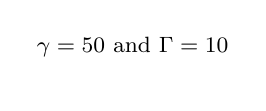
\begin{tikzpicture}[%
font=\footnotesize
]

\begin{axis}[%
width=0.951\figwidth,
height=\figheight,
at={(0\figwidth,0\figheight)},
scale only axis,
xmin=0,
xmax=3,
tick align=outside,
xlabel={Log-Moneyness},
xmajorgrids,
ymin=0,
ymax=5,
ylabel={Remaining Time},
ymajorgrids,
zmin=0,
zmax=0.08,
zlabel={Relative Increase},
zmajorgrids,
view={50}{40},
axis background/.style={fill=white},
title={$\gamma = 50$ and $\Gamma = 10$},
axis x line*=bottom,
axis y line*=left,
axis z line*=left
]

\addplot3[%
surf,
shader=flat corner,draw=black,z buffer=sort,colormap={mymap}{[1pt] rgb(0pt)=(0.2081,0.1663,0.5292); rgb(1pt)=(0.211624,0.189781,0.577676); rgb(2pt)=(0.212252,0.213771,0.626971); rgb(3pt)=(0.2081,0.2386,0.677086); rgb(4pt)=(0.195905,0.264457,0.7279); rgb(5pt)=(0.170729,0.291938,0.779248); rgb(6pt)=(0.125271,0.324243,0.830271); rgb(7pt)=(0.0591333,0.359833,0.868333); rgb(8pt)=(0.0116952,0.38751,0.881957); rgb(9pt)=(0.00595714,0.408614,0.882843); rgb(10pt)=(0.0165143,0.4266,0.878633); rgb(11pt)=(0.0328524,0.443043,0.871957); rgb(12pt)=(0.0498143,0.458571,0.864057); rgb(13pt)=(0.0629333,0.47369,0.855438); rgb(14pt)=(0.0722667,0.488667,0.8467); rgb(15pt)=(0.0779429,0.503986,0.838371); rgb(16pt)=(0.0793476,0.520024,0.831181); rgb(17pt)=(0.0749429,0.537543,0.826271); rgb(18pt)=(0.0640571,0.556986,0.823957); rgb(19pt)=(0.0487714,0.577224,0.822829); rgb(20pt)=(0.0343429,0.596581,0.819852); rgb(21pt)=(0.0265,0.6137,0.8135); rgb(22pt)=(0.0238905,0.628662,0.803762); rgb(23pt)=(0.0230905,0.641786,0.791267); rgb(24pt)=(0.0227714,0.653486,0.776757); rgb(25pt)=(0.0266619,0.664195,0.760719); rgb(26pt)=(0.0383714,0.674271,0.743552); rgb(27pt)=(0.0589714,0.683757,0.725386); rgb(28pt)=(0.0843,0.692833,0.706167); rgb(29pt)=(0.113295,0.7015,0.685857); rgb(30pt)=(0.145271,0.709757,0.664629); rgb(31pt)=(0.180133,0.717657,0.642433); rgb(32pt)=(0.217829,0.725043,0.619262); rgb(33pt)=(0.258643,0.731714,0.595429); rgb(34pt)=(0.302171,0.737605,0.571186); rgb(35pt)=(0.348167,0.742433,0.547267); rgb(36pt)=(0.395257,0.7459,0.524443); rgb(37pt)=(0.44201,0.748081,0.503314); rgb(38pt)=(0.487124,0.749062,0.483976); rgb(39pt)=(0.530029,0.749114,0.466114); rgb(40pt)=(0.570857,0.748519,0.44939); rgb(41pt)=(0.609852,0.747314,0.433686); rgb(42pt)=(0.6473,0.7456,0.4188); rgb(43pt)=(0.683419,0.743476,0.404433); rgb(44pt)=(0.71841,0.741133,0.390476); rgb(45pt)=(0.752486,0.7384,0.376814); rgb(46pt)=(0.785843,0.735567,0.363271); rgb(47pt)=(0.818505,0.732733,0.34979); rgb(48pt)=(0.850657,0.7299,0.336029); rgb(49pt)=(0.882433,0.727433,0.3217); rgb(50pt)=(0.913933,0.725786,0.306276); rgb(51pt)=(0.944957,0.726114,0.288643); rgb(52pt)=(0.973895,0.731395,0.266648); rgb(53pt)=(0.993771,0.745457,0.240348); rgb(54pt)=(0.999043,0.765314,0.216414); rgb(55pt)=(0.995533,0.786057,0.196652); rgb(56pt)=(0.988,0.8066,0.179367); rgb(57pt)=(0.978857,0.827143,0.163314); rgb(58pt)=(0.9697,0.848138,0.147452); rgb(59pt)=(0.962586,0.870514,0.1309); rgb(60pt)=(0.958871,0.8949,0.113243); rgb(61pt)=(0.959824,0.921833,0.0948381); rgb(62pt)=(0.9661,0.951443,0.0755333); rgb(63pt)=(0.9763,0.9831,0.0538)},mesh/rows=25]
table[row sep=crcr, point meta=\thisrow{c}] {%
%
x	y	z	c\\
0	0.01	0.00337541422359655	0.00337541422359655\\
0	0.111836734693878	0.0391363447716361	0.0391363447716361\\
0	0.213673469387755	0.0555803219726671	0.0555803219726671\\
0	0.315510204081633	0.060361171727477	0.060361171727477\\
0	0.41734693877551	0.0617622669699823	0.0617622669699823\\
0	0.519183673469388	0.0621985392443854	0.0621985392443854\\
0	0.621020408163265	0.0623407432311373	0.0623407432311373\\
0	0.722857142857143	0.0623884518812141	0.0623884518812141\\
0	0.82469387755102	0.0624047470650921	0.0624047470650921\\
0	0.926530612244898	0.062410377356836	0.062410377356836\\
0	1.02836734693878	0.0624123380619597	0.0624123380619597\\
0	1.13020408163265	0.062413024728227	0.062413024728227\\
0	1.23204081632653	0.0624132662335977	0.0624132662335977\\
0	1.33387755102041	0.0624133514558453	0.0624133514558453\\
0	1.43571428571429	0.0624133816095575	0.0624133816095575\\
0	1.53755102040816	0.0624133923021773	0.0624133923021773\\
0	1.63938775510204	0.0624133961007972	0.0624133961007972\\
0	1.74122448979592	0.0624133974523875	0.0624133974523875\\
0	1.8430612244898	0.0624133979339696	0.0624133979339696\\
0	1.94489795918367	0.0624133981057056	0.0624133981057056\\
0	2.04673469387755	0.0624133981670305	0.0624133981670305\\
0	2.14857142857143	0.0624133981889455	0.0624133981889455\\
0	2.25040816326531	0.0624133981968406	0.0624133981968406\\
0	2.35224489795918	0.0624133981996416	0.0624133981996416\\
0	2.45408163265306	0.0624133982005862	0.0624133982005862\\
0	2.55591836734694	0.0624133982009933	0.0624133982009933\\
0	2.65775510204082	0.0624133982011188	0.0624133982011188\\
0	2.75959183673469	0.0624133982012047	0.0624133982012047\\
0	2.86142857142857	0.0624133982011697	0.0624133982011697\\
0	2.96326530612245	0.0624133982011722	0.0624133982011722\\
0	3.06510204081633	0.0624133982012161	0.0624133982012161\\
0	3.1669387755102	0.0624133982011642	0.0624133982011642\\
0	3.26877551020408	0.0624133982011622	0.0624133982011622\\
0	3.37061224489796	0.0624133982012022	0.0624133982012022\\
0	3.47244897959184	0.0624133982011952	0.0624133982011952\\
0	3.57428571428571	0.0624133982011497	0.0624133982011497\\
0	3.67612244897959	0.0624133982011876	0.0624133982011876\\
0	3.77795918367347	0.0624133982011848	0.0624133982011848\\
0	3.87979591836735	0.0624133982012189	0.0624133982012189\\
0	3.98163265306122	0.0624133982011747	0.0624133982011747\\
0	4.0834693877551	0.0624133982012145	0.0624133982012145\\
0	4.18530612244898	0.0624133982011654	0.0624133982011654\\
0	4.28714285714286	0.0624133982011305	0.0624133982011305\\
0	4.38897959183674	0.0624133982012357	0.0624133982012357\\
0	4.49081632653061	0.0624133982011939	0.0624133982011939\\
0	4.59265306122449	0.0624133982011543	0.0624133982011543\\
0	4.69448979591837	0.0624133982011898	0.0624133982011898\\
0	4.79632653061224	0.0624133982011432	0.0624133982011432\\
0	4.89816326530612	0.0624133982011834	0.0624133982011834\\
0	5	0.0624133982012107	0.0624133982012107\\
0.125	0.01	1.24558506108898e-05	1.24558506108898e-05\\
0.125	0.111836734693878	0.00855296989138964	0.00855296989138964\\
0.125	0.213673469387755	0.0167661795082669	0.0167661795082669\\
0.125	0.315510204081633	0.0200041539426403	0.0200041539426403\\
0.125	0.41734693877551	0.0211137549392734	0.0211137549392734\\
0.125	0.519183673469388	0.0214882497894333	0.0214882497894333\\
0.125	0.621020408163265	0.0216155071835967	0.0216155071835967\\
0.125	0.722857142857143	0.0216591696800475	0.0216591696800475\\
0.125	0.82469387755102	0.0216742787111704	0.0216742787111704\\
0.125	0.926530612244898	0.0216795429050218	0.0216795429050218\\
0.125	1.02836734693878	0.0216813868674744	0.0216813868674744\\
0.125	1.13020408163265	0.0216820355016941	0.0216820355016941\\
0.125	1.23204081632653	0.0216822644320054	0.0216822644320054\\
0.125	1.33387755102041	0.0216823454527205	0.0216823454527205\\
0.125	1.43571428571429	0.0216823741954243	0.0216823741954243\\
0.125	1.53755102040816	0.0216823844160368	0.0216823844160368\\
0.125	1.63938775510204	0.0216823880577019	0.0216823880577019\\
0.125	1.74122448979592	0.0216823893358816	0.0216823893358816\\
0.125	1.8430612244898	0.0216823897981312	0.0216823897981312\\
0.125	1.94489795918367	0.02168238996324	0.02168238996324\\
0.125	2.04673469387755	0.0216823900222682	0.0216823900222682\\
0.125	2.14857142857143	0.02168239004339	0.02168239004339\\
0.125	2.25040816326531	0.0216823900509552	0.0216823900509552\\
0.125	2.35224489795918	0.0216823900536669	0.0216823900536669\\
0.125	2.45408163265306	0.0216823900546368	0.0216823900546368\\
0.125	2.55591836734694	0.0216823900549773	0.0216823900549773\\
0.125	2.65775510204082	0.0216823901624063	0.0216823901624063\\
0.125	2.75959183673469	0.0216823900551081	0.0216823900551081\\
0.125	2.86142857142857	0.0216823900550991	0.0216823900550991\\
0.125	2.96326530612245	0.0216823900550856	0.0216823900550856\\
0.125	3.06510204081633	0.0216823900550839	0.0216823900550839\\
0.125	3.1669387755102	0.0216823900551062	0.0216823900551062\\
0.125	3.26877551020408	0.0216823900551603	0.0216823900551603\\
0.125	3.37061224489796	0.0216823900552481	0.0216823900552481\\
0.125	3.47244897959184	0.0216823900553653	0.0216823900553653\\
0.125	3.57428571428571	0.0216823900554997	0.0216823900554997\\
0.125	3.67612244897959	0.021682390055632	0.021682390055632\\
0.125	3.77795918367347	0.0216823900557384	0.0216823900557384\\
0.125	3.87979591836735	0.021682390055792	0.021682390055792\\
0.125	3.98163265306122	0.0216823900557674	0.0216823900557674\\
0.125	4.0834693877551	0.0216823900556431	0.0216823900556431\\
0.125	4.18530612244898	0.0216823900554056	0.0216823900554056\\
0.125	4.28714285714286	0.0216823900550516	0.0216823900550516\\
0.125	4.38897959183674	0.02168239005459	0.02168239005459\\
0.125	4.49081632653061	0.0216823900540428	0.0216823900540428\\
0.125	4.59265306122449	0.0216823900534437	0.0216823900534437\\
0.125	4.69448979591837	0.0216823900528374	0.0216823900528374\\
0.125	4.79632653061224	0.0216823900522769	0.0216823900522769\\
0.125	4.89816326530612	0.0216823900518196	0.0216823900518196\\
0.125	5	0.0216823900515243	0.0216823900515243\\
0.25	0.01	3.20201401650257e-10	3.20201401650257e-10\\
0.25	0.111836734693878	0.00139574723125019	0.00139574723125019\\
0.25	0.213673469387755	0.00453277252368746	0.00453277252368746\\
0.25	0.315510204081633	0.00633956608890703	0.00633956608890703\\
0.25	0.41734693877551	0.00709057772059579	0.00709057772059579\\
0.25	0.519183673469388	0.00737313963463697	0.00737313963463697\\
0.25	0.621020408163265	0.00747560790903322	0.00747560790903322\\
0.25	0.722857142857143	0.00751224120120626	0.00751224120120626\\
0.25	0.82469387755102	0.0075252712963854	0.0075252712963854\\
0.25	0.926530612244898	0.00752990010711766	0.00752990010711766\\
0.25	1.02836734693878	0.00753154496040809	0.00753154496040809\\
0.25	1.13020408163265	0.00753212999715329	0.00753212999715329\\
0.25	1.23204081632653	0.0075323383116103	0.0075323383116103\\
0.25	1.33387755102041	0.0075324125686727	0.0075324125686727\\
0.25	1.43571428571429	0.00753243906658612	0.00753243906658612\\
0.25	1.53755102040816	0.00753244853121779	0.00753244853121779\\
0.25	1.63938775510204	0.00753245191478502	0.00753245191478502\\
0.25	1.74122448979592	0.00753245312534894	0.00753245312534894\\
0.25	1.8430612244898	0.00753245355876841	0.00753245355876841\\
0.25	1.94489795918367	0.00753245371404576	0.00753245371404576\\
0.25	2.04673469387755	0.00753245376970964	0.00753245376970964\\
0.25	2.14857142857143	0.00753245378967777	0.00753245378967777\\
0.25	2.25040816326531	0.00753245379684775	0.00753245379684775\\
0.25	2.35224489795918	0.00753245379942443	0.00753245379942443\\
0.25	2.45408163265306	0.00753245380034652	0.00753245380034652\\
0.25	2.55591836734694	0.00753245380066503	0.00753245380066503\\
0.25	2.65775510204082	0.0075324538007562	0.0075324538007562\\
0.25	2.75959183673469	0.00753245380075814	0.00753245380075814\\
0.25	2.86142857142857	0.00753245380072801	0.00753245380072801\\
0.25	2.96326530612245	0.00753245380069763	0.00753245380069763\\
0.25	3.06510204081633	0.00753245380069118	0.00753245380069118\\
0.25	3.1669387755102	0.00753245380072898	0.00753245380072898\\
0.25	3.26877551020408	0.00753245380082506	0.00753245380082506\\
0.25	3.37061224489796	0.00753245380098382	0.00753245380098382\\
0.25	3.47244897959184	0.00753245380119727	0.00753245380119727\\
0.25	3.57428571428571	0.00753245380144348	0.00753245380144348\\
0.25	3.67612244897959	0.00753245380168752	0.00753245380168752\\
0.25	3.77795918367347	0.0075324538018848	0.0075324538018848\\
0.25	3.87979591836735	0.00753245380198568	0.00753245380198568\\
0.25	3.98163265306122	0.00753245380194204	0.00753245380194204\\
0.25	4.0834693877551	0.00753245380171352	0.00753245380171352\\
0.25	4.18530612244898	0.00753245380127413	0.00753245380127413\\
0.25	4.28714285714286	0.00753245380084873	0.00753245380084873\\
0.25	4.38897959183674	0.0075324538008487	0.0075324538008487\\
0.25	4.49081632653061	0.00753245380084873	0.00753245380084873\\
0.25	4.59265306122449	0.00753245380084875	0.00753245380084875\\
0.25	4.69448979591837	0.0075324538008487	0.0075324538008487\\
0.25	4.79632653061224	0.00753245380084872	0.00753245380084872\\
0.25	4.89816326530612	0.0075324538008487	0.0075324538008487\\
0.25	5	0.00753245380084874	0.00753245380084874\\
0.375	0.01	2.53819448543796e-17	2.53819448543796e-17\\
0.375	0.111836734693878	0.000160070258810582	0.000160070258810582\\
0.375	0.213673469387755	0.00106113850625697	0.00106113850625697\\
0.375	0.315510204081633	0.00188035512787068	0.00188035512787068\\
0.375	0.41734693877551	0.00231183178163289	0.00231183178163289\\
0.375	0.519183673469388	0.00249841641175987	0.00249841641175987\\
0.375	0.621020408163265	0.00257234108940504	0.00257234108940504\\
0.375	0.722857142857143	0.00260038895098483	0.00260038895098483\\
0.375	0.82469387755102	0.00261079097852719	0.00261079097852719\\
0.375	0.926530612244898	0.00261460079488018	0.00261460079488018\\
0.375	1.02836734693878	0.00261598627870913	0.00261598627870913\\
0.375	1.13020408163265	0.00261648803323285	0.00261648803323285\\
0.375	1.23204081632653	0.00261666929225665	0.00261666929225665\\
0.375	1.33387755102041	0.002616734673377	0.002616734673377\\
0.375	1.43571428571429	0.00261675823508951	0.00261675823508951\\
0.375	1.53755102040816	0.00261676672144608	0.00261676672144608\\
0.375	1.63938775510204	0.00261676977702702	0.00261676977702702\\
0.375	1.74122448979592	0.00261677087724554	0.00261677087724554\\
0.375	1.8430612244898	0.00261677127325755	0.00261677127325755\\
0.375	1.94489795918367	0.00261677141581826	0.00261677141581826\\
0.375	2.04673469387755	0.00261677146714147	0.00261677146714147\\
0.375	2.14857142857143	0.00261677148691344	0.00261677148691344\\
0.375	2.25040816326531	0.00261677149227334	0.00261677149227334\\
0.375	2.35224489795918	0.00261677149466937	0.00261677149466937\\
0.375	2.45408163265306	0.00261677149553231	0.00261677149553231\\
0.375	2.55591836734694	0.00261677149584313	0.00261677149584313\\
0.375	2.65775510204082	0.0026167714959551	0.0026167714959551\\
0.375	2.75959183673469	0.00261677149599544	0.00261677149599544\\
0.375	2.86142857142857	0.00261677149600998	0.00261677149600998\\
0.375	2.96326530612245	0.00261677149601524	0.00261677149601524\\
0.375	3.06510204081633	0.00261677149601713	0.00261677149601713\\
0.375	3.1669387755102	0.00261677149601785	0.00261677149601785\\
0.375	3.26877551020408	0.00261677149601814	0.00261677149601814\\
0.375	3.37061224489796	0.00261677149601824	0.00261677149601824\\
0.375	3.47244897959184	0.00261677149601827	0.00261677149601827\\
0.375	3.57428571428571	0.00261677149601822	0.00261677149601822\\
0.375	3.67612244897959	0.00261677149601804	0.00261677149601804\\
0.375	3.77795918367347	0.00261677149601777	0.00261677149601777\\
0.375	3.87979591836735	0.00261677149601737	0.00261677149601737\\
0.375	3.98163265306122	0.00261677149601691	0.00261677149601691\\
0.375	4.0834693877551	0.00261677149601644	0.00261677149601644\\
0.375	4.18530612244898	0.00261677149601612	0.00261677149601612\\
0.375	4.28714285714286	0.00261677149601606	0.00261677149601606\\
0.375	4.38897959183674	0.00261677149601647	0.00261677149601647\\
0.375	4.49081632653061	0.00261677149601753	0.00261677149601753\\
0.375	4.59265306122449	0.00261677149601936	0.00261677149601936\\
0.375	4.69448979591837	0.00261677149602199	0.00261677149602199\\
0.375	4.79632653061224	0.00261677149602541	0.00261677149602541\\
0.375	4.89816326530612	0.00261677149602943	0.00261677149602943\\
0.375	5	0.00261677149603375	0.00261677149603375\\
0.5	0.01	4.83825345389175e-27	4.83825345389175e-27\\
0.5	0.111836734693878	1.22946045069483e-05	1.22946045069483e-05\\
0.5	0.213673469387755	0.000208898519576305	0.000208898519576305\\
0.5	0.315510204081633	0.000510807005794978	0.000510807005794978\\
0.5	0.41734693877551	0.000721484228630128	0.000721484228630128\\
0.5	0.519183673469388	0.00082939527154464	0.00082939527154464\\
0.5	0.621020408163265	0.000877158690074349	0.000877158690074349\\
0.5	0.722857142857143	0.000896724832081595	0.000896724832081595\\
0.5	0.82469387755102	0.000904393981253966	0.000904393981253966\\
0.5	0.926530612244898	0.000907321257420598	0.000907321257420598\\
0.5	1.02836734693878	0.000908420111470974	0.000908420111470974\\
0.5	1.13020408163265	0.000908828140823812	0.000908828140823812\\
0.5	1.23204081632653	0.000908978542824618	0.000908978542824618\\
0.5	1.33387755102041	0.000909033699536896	0.000909033699536896\\
0.5	1.43571428571429	0.000909053853523498	0.000909053853523498\\
0.5	1.53755102040816	0.000909061198142116	0.000909061198142116\\
0.5	1.63938775510204	0.000909063869420415	0.000909063869420415\\
0.5	1.74122448979592	0.000909064839528328	0.000909064839528328\\
0.5	1.8430612244898	0.000909065191431572	0.000909065191431572\\
0.5	1.94489795918367	0.00090906531897057	0.00090906531897057\\
0.5	2.04673469387755	0.000909065365164519	0.000909065365164519\\
0.5	2.14857142857143	0.000909065381891096	0.000909065381891096\\
0.5	2.25040816326531	0.000909065387949755	0.000909065387949755\\
0.5	2.35224489795918	0.000909065390144736	0.000909065390144736\\
0.5	2.45408163265306	0.000909065390933159	0.000909065390933159\\
0.5	2.55591836734694	0.000909065391199034	0.000909065391199034\\
0.5	2.65775510204082	0.000909065391260838	0.000909065391260838\\
0.5	2.75959183673469	0.000909065391339331	0.000909065391339331\\
0.5	2.86142857142857	0.00090906539135283	0.00090906539135283\\
0.5	2.96326530612245	0.000909065391357711	0.000909065391357711\\
0.5	3.06510204081633	0.000909065391359469	0.000909065391359469\\
0.5	3.1669387755102	0.000909065391360108	0.000909065391360108\\
0.5	3.26877551020408	0.000909065391360341	0.000909065391360341\\
0.5	3.37061224489796	0.00090906539136042	0.00090906539136042\\
0.5	3.47244897959184	0.000909065391360451	0.000909065391360451\\
0.5	3.57428571428571	0.000909065391360464	0.000909065391360464\\
0.5	3.67612244897959	0.000909065391360465	0.000909065391360465\\
0.5	3.77795918367347	0.000909065392925312	0.000909065392925312\\
0.5	3.87979591836735	0.000909065391360465	0.000909065391360465\\
0.5	3.98163265306122	0.000909065391360468	0.000909065391360468\\
0.5	4.0834693877551	0.000909065391360468	0.000909065391360468\\
0.5	4.18530612244898	0.000909065391360471	0.000909065391360471\\
0.5	4.28714285714286	0.000909065391360467	0.000909065391360467\\
0.5	4.38897959183674	0.000909065391360464	0.000909065391360464\\
0.5	4.49081632653061	0.000909065391360466	0.000909065391360466\\
0.5	4.59265306122449	0.000909065391360468	0.000909065391360468\\
0.5	4.69448979591837	0.000909065391360463	0.000909065391360463\\
0.5	4.79632653061224	0.000909065391360463	0.000909065391360463\\
0.5	4.89816326530612	0.000909065391360461	0.000909065391360461\\
0.5	5	0.000909065391360466	0.000909065391360466\\
0.625	0.01	2.01720632991655e-39	2.01720632991655e-39\\
0.625	0.111836734693878	6.09328988419564e-07	6.09328988419564e-07\\
0.625	0.213673469387755	3.3779937624515e-05	3.3779937624515e-05\\
0.625	0.315510204081633	0.000124625740345415	0.000124625740345415\\
0.625	0.41734693877551	0.000212304475351591	0.000212304475351591\\
0.625	0.519183673469388	0.000267075564141756	0.000267075564141756\\
0.625	0.621020408163265	0.000294737921422387	0.000294737921422387\\
0.625	0.722857142857143	0.000307172385326944	0.000307172385326944\\
0.625	0.82469387755102	0.000312389540277077	0.000312389540277077\\
0.625	0.926530612244898	0.000314486196342418	0.000314486196342418\\
0.625	1.02836734693878	0.000315305405868367	0.000315305405868367\\
0.625	1.13020408163265	0.000315619438221936	0.000315619438221936\\
0.625	1.23204081632653	0.000315738220462366	0.000315738220462366\\
0.625	1.33387755102041	0.000315782719536974	0.000315782719536974\\
0.625	1.43571428571429	0.000315799272181648	0.000315799272181648\\
0.625	1.53755102040816	0.000315805396514275	0.000315805396514275\\
0.625	1.63938775510204	0.000315807653158932	0.000315807653158932\\
0.625	1.74122448979592	0.000315808481999712	0.000315808481999712\\
0.625	1.8430612244898	0.000315808785648557	0.000315808785648557\\
0.625	1.94489795918367	0.000315808896663785	0.000315808896663785\\
0.625	2.04673469387755	0.000315808937183903	0.000315808937183903\\
0.625	2.14857142857143	0.000315808951953411	0.000315808951953411\\
0.625	2.25040816326531	0.000315808957330808	0.000315808957330808\\
0.625	2.35224489795918	0.000315808959286808	0.000315808959286808\\
0.625	2.45408163265306	0.000315808959997664	0.000315808959997664\\
0.625	2.55591836734694	0.000315808960255649	0.000315808960255649\\
0.625	2.65775510204082	0.000315808960348918	0.000315808960348918\\
0.625	2.75959183673469	0.000315808960382266	0.000315808960382266\\
0.625	2.86142857142857	0.00031580896039396	0.00031580896039396\\
0.625	2.96326530612245	0.00031580896039823	0.00031580896039823\\
0.625	3.06510204081633	0.000315808960400631	0.000315808960400631\\
0.625	3.1669387755102	0.000315808960403515	0.000315808960403515\\
0.625	3.26877551020408	0.000315808960407825	0.000315808960407825\\
0.625	3.37061224489796	0.000315808960413613	0.000315808960413613\\
0.625	3.47244897959184	0.00031580896042013	0.00031580896042013\\
0.625	3.57428571428571	0.000315808960425858	0.000315808960425858\\
0.625	3.67612244897959	0.000315808960428655	0.000315808960428655\\
0.625	3.77795918367347	0.000315808960426056	0.000315808960426056\\
0.625	3.87979591836735	0.000315808960415702	0.000315808960415702\\
0.625	3.98163265306122	0.00031580896040287	0.00031580896040287\\
0.625	4.0834693877551	0.00031580896040287	0.00031580896040287\\
0.625	4.18530612244898	0.00031580896040287	0.00031580896040287\\
0.625	4.28714285714286	0.000315808960402869	0.000315808960402869\\
0.625	4.38897959183674	0.000315808960402868	0.000315808960402868\\
0.625	4.49081632653061	0.000315808960402869	0.000315808960402869\\
0.625	4.59265306122449	0.00031580896040287	0.00031580896040287\\
0.625	4.69448979591837	0.000315808960402869	0.000315808960402869\\
0.625	4.79632653061224	0.000315808960402869	0.000315808960402869\\
0.625	4.89816326530612	0.000315808960402868	0.000315808960402868\\
0.625	5	0.000315808960402869	0.000315808960402869\\
0.75	0.01	1.75903541621462e-54	1.75903541621462e-54\\
0.75	0.111836734693878	1.89426367935576e-08	1.89426367935576e-08\\
0.75	0.213673469387755	4.4053446904925e-06	4.4053446904925e-06\\
0.75	0.315510204081633	2.6862130896185e-05	2.6862130896185e-05\\
0.75	0.41734693877551	5.80626809264906e-05	5.80626809264906e-05\\
0.75	0.519183673469388	8.25115121000702e-05	8.25115121000702e-05\\
0.75	0.621020408163265	9.68901799875422e-05	9.68901799875422e-05\\
0.75	0.722857142857143	0.000104092440459614	0.000104092440459614\\
0.75	0.82469387755102	0.000107366606655617	0.000107366606655617\\
0.75	0.926530612244898	0.000108765586766421	0.000108765586766421\\
0.75	1.02836734693878	0.000109339100895437	0.000109339100895437\\
0.75	1.13020408163265	0.000109567571811921	0.000109567571811921\\
0.75	1.23204081632653	0.000109656745042283	0.000109656745042283\\
0.75	1.33387755102041	0.000109691031878845	0.000109691031878845\\
0.75	1.43571428571429	0.00010970406764611	0.00010970406764611\\
0.75	1.53755102040816	0.00010970898132646	0.00010970898132646\\
0.75	1.63938775510204	0.000109710821093416	0.000109710821093416\\
0.75	1.74122448979592	0.000109711506282708	0.000109711506282708\\
0.75	1.8430612244898	0.000109711760382494	0.000109711760382494\\
0.75	1.94489795918367	0.000109711854287768	0.000109711854287768\\
0.75	2.04673469387755	0.000109711888892475	0.000109711888892475\\
0.75	2.14857142857143	0.000109711901614308	0.000109711901614308\\
0.75	2.25040816326531	0.000109711906281976	0.000109711906281976\\
0.75	2.35224489795918	0.000109711907991674	0.000109711907991674\\
0.75	2.45408163265306	0.000109711908617015	0.000109711908617015\\
0.75	2.55591836734694	0.000109711908845459	0.000109711908845459\\
0.75	2.65775510204082	0.000109711908928823	0.000109711908928823\\
0.75	2.75959183673469	0.000109711908959216	0.000109711908959216\\
0.75	2.86142857142857	0.000109711908970291	0.000109711908970291\\
0.75	2.96326530612245	0.000109711908974332	0.000109711908974332\\
0.75	3.06510204081633	0.000109711908975819	0.000109711908975819\\
0.75	3.1669387755102	0.000109711908976384	0.000109711908976384\\
0.75	3.26877551020408	0.000109711908976613	0.000109711908976613\\
0.75	3.37061224489796	0.000109711908976703	0.000109711908976703\\
0.75	3.47244897959184	0.000109711908976706	0.000109711908976706\\
0.75	3.57428571428571	0.000109711908976615	0.000109711908976615\\
0.75	3.67612244897959	0.000109711908976409	0.000109711908976409\\
0.75	3.77795918367347	0.000109711908976077	0.000109711908976077\\
0.75	3.87979591836735	0.000109711908975636	0.000109711908975636\\
0.75	3.98163265306122	0.000109711908975149	0.000109711908975149\\
0.75	4.0834693877551	0.000109711908974727	0.000109711908974727\\
0.75	4.18530612244898	0.000109711908974528	0.000109711908974528\\
0.75	4.28714285714286	0.000109711908976626	0.000109711908976626\\
0.75	4.38897959183674	0.000109711908976626	0.000109711908976626\\
0.75	4.49081632653061	0.000109711908976626	0.000109711908976626\\
0.75	4.59265306122449	0.000109711908976627	0.000109711908976627\\
0.75	4.69448979591837	0.000109711908976626	0.000109711908976626\\
0.75	4.79632653061224	0.000109711908976626	0.000109711908976626\\
0.75	4.89816326530612	0.000109711908976626	0.000109711908976626\\
0.75	5	0.000109711908976627	0.000109711908976627\\
0.875	0.01	3.1307068490861e-72	3.1307068490861e-72\\
0.875	0.111836734693878	3.61624088332981e-10	3.61624088332981e-10\\
0.875	0.213673469387755	4.56778427822024e-07	4.56778427822024e-07\\
0.875	0.315510204081633	5.0476132191807e-06	5.0476132191807e-06\\
0.875	0.41734693877551	1.45709663209533e-05	1.45709663209533e-05\\
0.875	0.519183673469388	2.41883302163219e-05	2.41883302163219e-05\\
0.875	0.621020408163265	3.0904949996867e-05	3.0904949996867e-05\\
0.875	0.722857142857143	3.47098240413525e-05	3.47098240413525e-05\\
0.875	0.82469387755102	3.66058295473457e-05	3.66058295473457e-05\\
0.875	0.926530612244898	3.74752597275394e-05	3.74752597275394e-05\\
0.875	1.02836734693878	3.78521163970537e-05	3.78521163970537e-05\\
0.875	1.13020408163265	3.80091378092108e-05	3.80091378092108e-05\\
0.875	1.23204081632653	3.80727206230729e-05	3.80727206230729e-05\\
0.875	1.33387755102041	3.80979279417586e-05	3.80979279417586e-05\\
0.875	1.43571428571429	3.81077622877283e-05	3.81077622877283e-05\\
0.875	1.53755102040816	3.81115517686971e-05	3.81115517686971e-05\\
0.875	1.63938775510204	3.81129978112158e-05	3.81129978112158e-05\\
0.875	1.74122448979592	3.81135453360158e-05	3.81135453360158e-05\\
0.875	1.8430612244898	3.81137513482524e-05	3.81137513482524e-05\\
0.875	1.94489795918367	3.81138284641102e-05	3.81138284641102e-05\\
0.875	2.04673469387755	3.81138572077087e-05	3.81138572077087e-05\\
0.875	2.14857142857143	3.81138678832337e-05	3.81138678832337e-05\\
0.875	2.25040816326531	3.81138718362682e-05	3.81138718362682e-05\\
0.875	2.35224489795918	3.8113873296295e-05	3.8113873296295e-05\\
0.875	2.45408163265306	3.81138738343658e-05	3.81138738343658e-05\\
0.875	2.55591836734694	3.81138740322894e-05	3.81138740322894e-05\\
0.875	2.65775510204082	3.81138741049742e-05	3.81138741049742e-05\\
0.875	2.75959183673469	3.81138741316285e-05	3.81138741316285e-05\\
0.875	2.86142857142857	3.81138741413907e-05	3.81138741413907e-05\\
0.875	2.96326530612245	3.81138741449623e-05	3.81138741449623e-05\\
0.875	3.06510204081633	3.81138741462675e-05	3.81138741462675e-05\\
0.875	3.1669387755102	3.81138741467443e-05	3.81138741467443e-05\\
0.875	3.26877551020408	3.81138741469183e-05	3.81138741469183e-05\\
0.875	3.37061224489796	3.81138741469814e-05	3.81138741469814e-05\\
0.875	3.47244897959184	3.81138741470039e-05	3.81138741470039e-05\\
0.875	3.57428571428571	3.81138741470115e-05	3.81138741470115e-05\\
0.875	3.67612244897959	3.81138741470135e-05	3.81138741470135e-05\\
0.875	3.77795918367347	3.81138741470148e-05	3.81138741470148e-05\\
0.875	3.87979591836735	3.81138741470176e-05	3.81138741470176e-05\\
0.875	3.98163265306122	3.81138741470245e-05	3.81138741470245e-05\\
0.875	4.0834693877551	3.81138741470369e-05	3.81138741470369e-05\\
0.875	4.18530612244898	3.81138741470555e-05	3.81138741470555e-05\\
0.875	4.28714285714286	3.81138741470789e-05	3.81138741470789e-05\\
0.875	4.38897959183674	3.81138741471035e-05	3.81138741471035e-05\\
0.875	4.49081632653061	3.81138741471225e-05	3.81138741471225e-05\\
0.875	4.59265306122449	3.81138741471252e-05	3.81138741471252e-05\\
0.875	4.69448979591837	3.81138741470989e-05	3.81138741470989e-05\\
0.875	4.79632653061224	3.81138741470299e-05	3.81138741470299e-05\\
0.875	4.89816326530612	3.81138741469055e-05	3.81138741469055e-05\\
0.875	5	3.81138741467176e-05	3.81138741467176e-05\\
1	0.01	1.12056931755422e-92	1.12056931755422e-92\\
1	0.111836734693878	4.17271019572753e-12	4.17271019572753e-12\\
1	0.213673469387755	3.72382096859804e-08	3.72382096859804e-08\\
1	0.315510204081633	8.1823877822432e-07	8.1823877822432e-07\\
1	0.41734693877551	3.31935176812392e-06	3.31935176812392e-06\\
1	0.519183673469388	6.65939206175038e-06	6.65939206175038e-06\\
1	0.621020408163265	9.48248056092038e-06	9.48248056092038e-06\\
1	0.722857142857143	1.13172529427281e-05	1.13172529427281e-05\\
1	0.82469387755102	1.23307521957583e-05	1.23307521957583e-05\\
1	0.926530612244898	1.28340558530098e-05	1.28340558530098e-05\\
1	1.02836734693878	1.3066443724347e-05	1.3066443724347e-05\\
1	1.13020408163265	1.3168348826661e-05	1.3168348826661e-05\\
1	1.23204081632653	1.321138594121e-05	1.321138594121e-05\\
1	1.33387755102041	1.3229057753984e-05	1.3229057753984e-05\\
1	1.43571428571429	1.32361600216795e-05	1.32361600216795e-05\\
1	1.53755102040816	1.32389671438567e-05	1.32389671438567e-05\\
1	1.63938775510204	1.32400620848615e-05	1.32400620848615e-05\\
1	1.74122448979592	1.32404846735509e-05	1.32404846735509e-05\\
1	1.8430612244898	1.3240646370972e-05	1.3240646370972e-05\\
1	1.94489795918367	1.3240707805149e-05	1.3240707805149e-05\\
1	2.04673469387755	1.32407310088811e-05	1.32407310088811e-05\\
1	2.14857142857143	1.3240739729709e-05	1.3240739729709e-05\\
1	2.25040816326531	1.32407429936269e-05	1.32407429936269e-05\\
1	2.35224489795918	1.32407442108472e-05	1.32407442108472e-05\\
1	2.45408163265306	1.32407446633964e-05	1.32407446633964e-05\\
1	2.55591836734694	1.3240744831203e-05	1.3240744831203e-05\\
1	2.65775510204082	1.32407448932826e-05	1.32407448932826e-05\\
1	2.75959183673469	1.32407449162023e-05	1.32407449162023e-05\\
1	2.86142857142857	1.32407449246493e-05	1.32407449246493e-05\\
1	2.96326530612245	1.32407449277575e-05	1.32407449277575e-05\\
1	3.06510204081633	1.32407449288996e-05	1.32407449288996e-05\\
1	3.1669387755102	1.32407449293188e-05	1.32407449293188e-05\\
1	3.26877551020408	1.32407449294724e-05	1.32407449294724e-05\\
1	3.37061224489796	1.32407449295287e-05	1.32407449295287e-05\\
1	3.47244897959184	1.32407449295492e-05	1.32407449295492e-05\\
1	3.57428571428571	1.32407449295567e-05	1.32407449295567e-05\\
1	3.67612244897959	1.32407449295594e-05	1.32407449295594e-05\\
1	3.77795918367347	1.32407449295604e-05	1.32407449295604e-05\\
1	3.87979591836735	1.32407449295607e-05	1.32407449295607e-05\\
1	3.98163265306122	1.32407449295609e-05	1.32407449295609e-05\\
1	4.0834693877551	1.3240744929561e-05	1.3240744929561e-05\\
1	4.18530612244898	1.32407449295611e-05	1.32407449295611e-05\\
1	4.28714285714286	1.32407449295611e-05	1.32407449295611e-05\\
1	4.38897959183674	1.32407449295608e-05	1.32407449295608e-05\\
1	4.49081632653061	1.32407449295604e-05	1.32407449295604e-05\\
1	4.59265306122449	1.32407449295598e-05	1.32407449295598e-05\\
1	4.69448979591837	1.3240744929559e-05	1.3240744929559e-05\\
1	4.79632653061224	1.32407449295585e-05	1.32407449295585e-05\\
1	4.89816326530612	1.32407449295586e-05	1.32407449295586e-05\\
1	5	1.32407449295601e-05	1.32407449295601e-05\\
1.125	0.01	7.98909245102218e-116	7.98909245102218e-116\\
1.125	0.111836734693878	2.87598750129709e-14	2.87598750129709e-14\\
1.125	0.213673469387755	2.36590494241211e-09	2.36590494241211e-09\\
1.125	0.315510204081633	1.13481438981253e-07	1.13481438981253e-07\\
1.125	0.41734693877551	6.80408215513725e-07	6.80408215513725e-07\\
1.125	0.519183673469388	1.70630947588123e-06	1.70630947588123e-06\\
1.125	0.621020408163265	2.77522233746852e-06	2.77522233746852e-06\\
1.125	0.722857142857143	3.58344962789663e-06	3.58344962789663e-06\\
1.125	0.82469387755102	4.08378362937912e-06	4.08378362937912e-06\\
1.125	0.926530612244898	4.35523644773063e-06	4.35523644773063e-06\\
1.125	1.02836734693878	4.48971722606522e-06	4.48971722606522e-06\\
1.125	1.13020408163265	4.55215856569508e-06	4.55215856569508e-06\\
1.125	1.23204081632653	4.57980360325272e-06	4.57980360325272e-06\\
1.125	1.33387755102041	4.59161278327766e-06	4.59161278327766e-06\\
1.125	1.43571428571429	4.5965205995352e-06	4.5965205995352e-06\\
1.125	1.53755102040816	4.59851689978353e-06	4.59851689978353e-06\\
1.125	1.63938775510204	4.59931517049035e-06	4.59931517049035e-06\\
1.125	1.74122448979592	4.59963001834023e-06	4.59963001834023e-06\\
1.125	1.8430612244898	4.59975281202095e-06	4.59975281202095e-06\\
1.125	1.94489795918367	4.59980026102008e-06	4.59980026102008e-06\\
1.125	2.04673469387755	4.59981845476392e-06	4.59981845476392e-06\\
1.125	2.14857142857143	4.59982538570597e-06	4.59982538570597e-06\\
1.125	2.25040816326531	4.59982801152411e-06	4.59982801152411e-06\\
1.125	2.35224489795918	4.59982900163991e-06	4.59982900163991e-06\\
1.125	2.45408163265306	4.59982937346664e-06	4.59982937346664e-06\\
1.125	2.55591836734694	4.59982951261035e-06	4.59982951261035e-06\\
1.125	2.65775510204082	4.59982956452031e-06	4.59982956452031e-06\\
1.125	2.75959183673469	4.59982958383407e-06	4.59982958383407e-06\\
1.125	2.86142857142857	4.59982959100293e-06	4.59982959100293e-06\\
1.125	2.96326530612245	4.59982959365828e-06	4.59982959365828e-06\\
1.125	3.06510204081633	4.59982959463995e-06	4.59982959463995e-06\\
1.125	3.1669387755102	4.59982959500229e-06	4.59982959500229e-06\\
1.125	3.26877551020408	4.59982959513583e-06	4.59982959513583e-06\\
1.125	3.37061224489796	4.59982959518496e-06	4.59982959518496e-06\\
1.125	3.47244897959184	4.59982959520303e-06	4.59982959520303e-06\\
1.125	3.57428571428571	4.59982959520968e-06	4.59982959520968e-06\\
1.125	3.67612244897959	4.59982959521212e-06	4.59982959521212e-06\\
1.125	3.77795918367347	4.59982959521304e-06	4.59982959521304e-06\\
1.125	3.87979591836735	4.59982959521336e-06	4.59982959521336e-06\\
1.125	3.98163265306122	4.59982959521351e-06	4.59982959521351e-06\\
1.125	4.0834693877551	4.59982959521356e-06	4.59982959521356e-06\\
1.125	4.18530612244898	4.59982959521357e-06	4.59982959521357e-06\\
1.125	4.28714285714286	4.59982959521353e-06	4.59982959521353e-06\\
1.125	4.38897959183674	4.59982959521347e-06	4.59982959521347e-06\\
1.125	4.49081632653061	4.59982959521344e-06	4.59982959521344e-06\\
1.125	4.59265306122449	4.59982959521341e-06	4.59982959521341e-06\\
1.125	4.69448979591837	4.59982959521336e-06	4.59982959521336e-06\\
1.125	4.79632653061224	4.59982959521336e-06	4.59982959521336e-06\\
1.125	4.89816326530612	4.59982959521337e-06	4.59982959521337e-06\\
1.125	5	4.59982959521344e-06	4.59982959521344e-06\\
1.25	0.01	1.12709870060091e-141	1.12709870060091e-141\\
1.25	0.111836734693878	1.17358918998876e-16	1.17358918998876e-16\\
1.25	0.213673469387755	1.16324078317323e-10	1.16324078317323e-10\\
1.25	0.315510204081633	1.33773349726512e-08	1.33773349726512e-08\\
1.25	0.41734693877551	1.24613167678806e-07	1.24613167678806e-07\\
1.25	0.519183673469388	4.03770036875383e-07	4.03770036875383e-07\\
1.25	0.621020408163265	7.68755159782284e-07	7.68755159782284e-07\\
1.25	0.722857142857143	1.09423148340592e-06	1.09423148340592e-06\\
1.25	0.82469387755102	1.32245873561479e-06	1.32245873561479e-06\\
1.25	0.926530612244898	1.45890340087368e-06	1.45890340087368e-06\\
1.25	1.02836734693878	1.53194491804109e-06	1.53194491804109e-06\\
1.25	1.13020408163265	1.56806742051303e-06	1.56806742051303e-06\\
1.25	1.23204081632653	1.58491744647666e-06	1.58491744647666e-06\\
1.25	1.33387755102041	1.59243783982161e-06	1.59243783982161e-06\\
1.25	1.43571428571429	1.59568187572679e-06	1.59568187572679e-06\\
1.25	1.53755102040816	1.59704431064049e-06	1.59704431064049e-06\\
1.25	1.63938775510204	1.59760443439603e-06	1.59760443439603e-06\\
1.25	1.74122448979592	1.59783077571705e-06	1.59783077571705e-06\\
1.25	1.8430612244898	1.59792095649642e-06	1.59792095649642e-06\\
1.25	1.94489795918367	1.59795646976032e-06	1.59795646976032e-06\\
1.25	2.04673469387755	1.59797031899024e-06	1.59797031899024e-06\\
1.25	2.14857142857143	1.59797567550551e-06	1.59797567550551e-06\\
1.25	2.25040816326531	1.59797773279458e-06	1.59797773279458e-06\\
1.25	2.35224489795918	1.59797851821052e-06	1.59797851821052e-06\\
1.25	2.45408163265306	1.59797881651039e-06	1.59797881651039e-06\\
1.25	2.55591836734694	1.59797892929544e-06	1.59797892929544e-06\\
1.25	2.65775510204082	1.59797897177134e-06	1.59797897177134e-06\\
1.25	2.75959183673469	1.59797898771302e-06	1.59797898771302e-06\\
1.25	2.86142857142857	1.5979789936779e-06	1.5979789936779e-06\\
1.25	2.96326530612245	1.59797899590377e-06	1.59797899590377e-06\\
1.25	3.06510204081633	1.59797899673237e-06	1.59797899673237e-06\\
1.25	3.1669387755102	1.59797899704017e-06	1.59797899704017e-06\\
1.25	3.26877551020408	1.59797899715429e-06	1.59797899715429e-06\\
1.25	3.37061224489796	1.59797899719652e-06	1.59797899719652e-06\\
1.25	3.47244897959184	1.59797899721213e-06	1.59797899721213e-06\\
1.25	3.57428571428571	1.59797899721789e-06	1.59797899721789e-06\\
1.25	3.67612244897959	1.59797899722e-06	1.59797899722e-06\\
1.25	3.77795918367347	1.59797899722078e-06	1.59797899722078e-06\\
1.25	3.87979591836735	1.59797899722105e-06	1.59797899722105e-06\\
1.25	3.98163265306122	1.59797899722116e-06	1.59797899722116e-06\\
1.25	4.0834693877551	1.5979789972212e-06	1.5979789972212e-06\\
1.25	4.18530612244898	1.59797899722122e-06	1.59797899722122e-06\\
1.25	4.28714285714286	1.59797899722123e-06	1.59797899722123e-06\\
1.25	4.38897959183674	1.59797899722123e-06	1.59797899722123e-06\\
1.25	4.49081632653061	1.59797899722125e-06	1.59797899722125e-06\\
1.25	4.59265306122449	1.59797899722127e-06	1.59797899722127e-06\\
1.25	4.69448979591837	1.59797899722128e-06	1.59797899722128e-06\\
1.25	4.79632653061224	1.59797899722129e-06	1.59797899722129e-06\\
1.25	4.89816326530612	1.59797899722129e-06	1.59797899722129e-06\\
1.25	5	1.59797899722128e-06	1.59797899722128e-06\\
1.375	0.01	3.13176410675462e-170	3.13176410675462e-170\\
1.375	0.111836734693878	2.81644467419927e-19	2.81644467419927e-19\\
1.375	0.213673469387755	4.40085531216938e-12	4.40085531216938e-12\\
1.375	0.315510204081633	1.3333135625436e-09	1.3333135625436e-09\\
1.375	0.41734693877551	2.02757365220771e-08	2.02757365220771e-08\\
1.375	0.519183673469388	8.76800309016936e-08	8.76800309016936e-08\\
1.375	0.621020408163265	2.00184698145705e-07	2.00184698145705e-07\\
1.375	0.722857142857143	3.20092899756823e-07	3.20092899756823e-07\\
1.375	0.82469387755102	4.16334465016758e-07	4.16334465016758e-07\\
1.375	0.926530612244898	4.80272634621527e-07	4.80272634621527e-07\\
1.375	1.02836734693878	5.17513813574676e-07	5.17513813574676e-07\\
1.375	1.13020408163265	5.37244440661732e-07	5.37244440661732e-07\\
1.375	1.23204081632653	5.4698932711951e-07	5.4698932711951e-07\\
1.375	1.33387755102041	5.51552745368664e-07	5.51552745368664e-07\\
1.375	1.43571428571429	5.53603464563923e-07	5.53603464563923e-07\\
1.375	1.53755102040816	5.54495587261128e-07	5.54495587261128e-07\\
1.375	1.63938775510204	5.54873740038605e-07	5.54873740038605e-07\\
1.375	1.74122448979592	5.55030692532659e-07	5.55030692532659e-07\\
1.375	1.8430612244898	5.55094720136043e-07	5.55094720136043e-07\\
1.375	1.94489795918367	5.55120468098519e-07	5.55120468098519e-07\\
1.375	2.04673469387755	5.5513069878696e-07	5.5513069878696e-07\\
1.375	2.14857142857143	5.55134722807497e-07	5.55134722807497e-07\\
1.375	2.25040816326531	5.55136291943904e-07	5.55136291943904e-07\\
1.375	2.35224489795918	5.55136899292615e-07	5.55136899292615e-07\\
1.375	2.45408163265306	5.55137132869624e-07	5.55137132869624e-07\\
1.375	2.55591836734694	5.55137222200146e-07	5.55137222200146e-07\\
1.375	2.65775510204082	5.55137256197978e-07	5.55137256197978e-07\\
1.375	2.75959183673469	5.55137269081659e-07	5.55137269081659e-07\\
1.375	2.86142857142857	5.55137273945541e-07	5.55137273945541e-07\\
1.375	2.96326530612245	5.55137275775603e-07	5.55137275775603e-07\\
1.375	3.06510204081633	5.55137276462109e-07	5.55137276462109e-07\\
1.375	3.1669387755102	5.55137276718949e-07	5.55137276718949e-07\\
1.375	3.26877551020408	5.55137276814809e-07	5.55137276814809e-07\\
1.375	3.37061224489796	5.55137276850506e-07	5.55137276850506e-07\\
1.375	3.47244897959184	5.55137276863775e-07	5.55137276863775e-07\\
1.375	3.57428571428571	5.551372768687e-07	5.551372768687e-07\\
1.375	3.67612244897959	5.55137276870524e-07	5.55137276870524e-07\\
1.375	3.77795918367347	5.55137276871201e-07	5.55137276871201e-07\\
1.375	3.87979591836735	5.5513727687145e-07	5.5513727687145e-07\\
1.375	3.98163265306122	5.55137276871545e-07	5.55137276871545e-07\\
1.375	4.0834693877551	5.55137276871578e-07	5.55137276871578e-07\\
1.375	4.18530612244898	5.55137276871589e-07	5.55137276871589e-07\\
1.375	4.28714285714286	5.55137276871589e-07	5.55137276871589e-07\\
1.375	4.38897959183674	5.55137276871584e-07	5.55137276871584e-07\\
1.375	4.49081632653061	5.55137276871581e-07	5.55137276871581e-07\\
1.375	4.59265306122449	5.55137276871579e-07	5.55137276871579e-07\\
1.375	4.69448979591837	5.55137276871574e-07	5.55137276871574e-07\\
1.375	4.79632653061224	5.55137276871574e-07	5.55137276871574e-07\\
1.375	4.89816326530612	5.55137276871574e-07	5.55137276871574e-07\\
1.375	5	5.5513727687158e-07	5.5513727687158e-07\\
1.5	0.01	1.70791870631871e-201	1.70791870631871e-201\\
1.5	0.111836734693878	3.95483348479407e-22	3.95483348479407e-22\\
1.5	0.213673469387755	1.27524280956265e-13	1.27524280956265e-13\\
1.5	0.315510204081633	1.11883018336697e-10	1.11883018336697e-10\\
1.5	0.41734693877551	2.91764867131404e-09	2.91764867131404e-09\\
1.5	0.519183673469388	1.73821497755967e-08	1.73821497755967e-08\\
1.5	0.621020408163265	4.87192586292003e-08	4.87192586292003e-08\\
1.5	0.722857142857143	8.91597564554113e-08	8.91597564554113e-08\\
1.5	0.82469387755102	1.26696457208926e-07	1.26696457208926e-07\\
1.5	0.926530612244898	1.54638187154185e-07	1.54638187154185e-07\\
1.5	1.02836734693878	1.72466786245567e-07	1.72466786245567e-07\\
1.5	1.13020408163265	1.82643624316404e-07	1.82643624316404e-07\\
1.5	1.23204081632653	1.87991225316002e-07	1.87991225316002e-07\\
1.5	1.33387755102041	1.9062968025211e-07	1.9062968025211e-07\\
1.5	1.43571428571429	1.91869343520203e-07	1.91869343520203e-07\\
1.5	1.53755102040816	1.92429725312516e-07	1.92429725312516e-07\\
1.5	1.63938775510204	1.92675317120246e-07	1.92675317120246e-07\\
1.5	1.74122448979592	1.92780274578467e-07	1.92780274578467e-07\\
1.5	1.8430612244898	1.92824210921585e-07	1.92824210921585e-07\\
1.5	1.94489795918367	1.92842289451398e-07	1.92842289451398e-07\\
1.5	2.04673469387755	1.92849621614425e-07	1.92849621614425e-07\\
1.5	2.14857142857143	1.92852559215877e-07	1.92852559215877e-07\\
1.5	2.25040816326531	1.92853723942303e-07	1.92853723942303e-07\\
1.5	2.35224489795918	1.92854181621811e-07	1.92854181621811e-07\\
1.5	2.45408163265306	1.92854360077332e-07	1.92854360077332e-07\\
1.5	2.55591836734694	1.92854429191237e-07	1.92854429191237e-07\\
1.5	2.65775510204082	1.92854455800503e-07	1.92854455800503e-07\\
1.5	2.75959183673469	1.92854465992053e-07	1.92854465992053e-07\\
1.5	2.86142857142857	1.9285446987757e-07	1.9285446987757e-07\\
1.5	2.96326530612245	1.92854471352875e-07	1.92854471352875e-07\\
1.5	3.06510204081633	1.92854471910998e-07	1.92854471910998e-07\\
1.5	3.1669387755102	1.92854472121455e-07	1.92854472121455e-07\\
1.5	3.26877551020408	1.92854472200581e-07	1.92854472200581e-07\\
1.5	3.37061224489796	1.9285447223025e-07	1.9285447223025e-07\\
1.5	3.47244897959184	1.92854472241349e-07	1.92854472241349e-07\\
1.5	3.57428571428571	1.92854472245492e-07	1.92854472245492e-07\\
1.5	3.67612244897959	1.92854472247035e-07	1.92854472247035e-07\\
1.5	3.77795918367347	1.92854472247609e-07	1.92854472247609e-07\\
1.5	3.87979591836735	1.92854472247821e-07	1.92854472247821e-07\\
1.5	3.98163265306122	1.92854472247901e-07	1.92854472247901e-07\\
1.5	4.0834693877551	1.9285447224793e-07	1.9285447224793e-07\\
1.5	4.18530612244898	1.92854472247942e-07	1.92854472247942e-07\\
1.5	4.28714285714286	1.92854472247947e-07	1.92854472247947e-07\\
1.5	4.38897959183674	1.92854472247949e-07	1.92854472247949e-07\\
1.5	4.49081632653061	1.92854472247951e-07	1.92854472247951e-07\\
1.5	4.59265306122449	1.92854472247953e-07	1.92854472247953e-07\\
1.5	4.69448979591837	1.92854472247952e-07	1.92854472247952e-07\\
1.5	4.79632653061224	1.92854472247951e-07	1.92854472247951e-07\\
1.5	4.89816326530612	1.92854472247949e-07	1.92854472247949e-07\\
1.5	5	1.92854472247947e-07	1.92854472247947e-07\\
1.625	0.01	1.82325301139829e-235	1.82325301139829e-235\\
1.625	0.111836734693878	3.23660641934573e-25	3.23660641934573e-25\\
1.625	0.213673469387755	2.81964348776471e-15	2.81964348776471e-15\\
1.625	0.315510204081633	7.8767940747423e-12	7.8767940747423e-12\\
1.625	0.41734693877551	3.69943869214873e-10	3.69943869214873e-10\\
1.625	0.519183673469388	3.13265134452383e-09	3.13265134452383e-09\\
1.625	0.621020408163265	1.10277427258172e-08	1.10277427258172e-08\\
1.625	0.722857142857143	2.35218431231179e-08	2.35218431231179e-08\\
1.625	0.82469387755102	3.70690808581918e-08	3.70690808581918e-08\\
1.625	0.926530612244898	4.84606409597449e-08	4.84606409597449e-08\\
1.625	1.02836734693878	5.64765760105587e-08	5.64765760105587e-08\\
1.625	1.13020408163265	6.14340334115632e-08	6.14340334115632e-08\\
1.625	1.23204081632653	6.42187417098359e-08	6.42187417098359e-08\\
1.625	1.33387755102041	6.56722684502468e-08	6.56722684502468e-08\\
1.625	1.43571428571429	6.63888381270866e-08	6.63888381270866e-08\\
1.625	1.53755102040816	6.67264781605944e-08	6.67264781605944e-08\\
1.625	1.63938775510204	6.68798927840051e-08	6.68798927840051e-08\\
1.625	1.74122448979592	6.69475677789791e-08	6.69475677789791e-08\\
1.625	1.8430612244898	6.69767018899201e-08	6.69767018899201e-08\\
1.625	1.94489795918367	6.69889921179657e-08	6.69889921179657e-08\\
1.625	2.04673469387755	6.69940890476091e-08	6.69940890476091e-08\\
1.625	2.14857142857143	6.69961724625742e-08	6.69961724625742e-08\\
1.625	2.25040816326531	6.69970136170175e-08	6.69970136170175e-08\\
1.625	2.35224489795918	6.69973496306427e-08	6.69973496306427e-08\\
1.625	2.45408163265306	6.69974826261786e-08	6.69974826261786e-08\\
1.625	2.55591836734694	6.69975348454116e-08	6.69975348454116e-08\\
1.625	2.65775510204082	6.69975552049684e-08	6.69975552049684e-08\\
1.625	2.75959183673469	6.6997563093834e-08	6.6997563093834e-08\\
1.625	2.86142857142857	6.69975661338683e-08	6.69975661338683e-08\\
1.625	2.96326530612245	6.69975672996696e-08	6.69975672996696e-08\\
1.625	3.06510204081633	6.6997567744792e-08	6.6997567744792e-08\\
1.625	3.1669387755102	6.69975679140857e-08	6.69975679140857e-08\\
1.625	3.26877551020408	6.69975679782478e-08	6.69975679782478e-08\\
1.625	3.37061224489796	6.69975680024879e-08	6.69975680024879e-08\\
1.625	3.47244897959184	6.69975680116196e-08	6.69975680116196e-08\\
1.625	3.57428571428571	6.69975680150511e-08	6.69975680150511e-08\\
1.625	3.67612244897959	6.69975680163371e-08	6.69975680163371e-08\\
1.625	3.77795918367347	6.69975680168184e-08	6.69975680168184e-08\\
1.625	3.87979591836735	6.69975680169977e-08	6.69975680169977e-08\\
1.625	3.98163265306122	6.69975680170648e-08	6.69975680170648e-08\\
1.625	4.0834693877551	6.69975680170895e-08	6.69975680170895e-08\\
1.625	4.18530612244898	6.69975680170985e-08	6.69975680170985e-08\\
1.625	4.28714285714286	6.69975680171014e-08	6.69975680171014e-08\\
1.625	4.38897959183674	6.69975680171023e-08	6.69975680171023e-08\\
1.625	4.49081632653061	6.69975680171027e-08	6.69975680171027e-08\\
1.625	4.59265306122449	6.69975680171032e-08	6.69975680171032e-08\\
1.625	4.69448979591837	6.69975680171035e-08	6.69975680171035e-08\\
1.625	4.79632653061224	6.69975680171043e-08	6.69975680171043e-08\\
1.625	4.89816326530612	6.6997568017105e-08	6.6997568017105e-08\\
1.625	5	6.69975680171061e-08	6.69975680171061e-08\\
1.75	0.01	3.80219035229783e-272	3.80219035229783e-272\\
1.75	0.111836734693878	1.53905560924506e-28	1.53905560924506e-28\\
1.75	0.213673469387755	4.74228723894123e-17	4.74228723894123e-17\\
1.75	0.315510204081633	4.63907789088628e-13	4.63907789088628e-13\\
1.75	0.41734693877551	4.1207895061965e-11	4.1207895061965e-11\\
1.75	0.519183673469388	5.1149129131191e-10	5.1149129131191e-10\\
1.75	0.621020408163265	2.31230212247965e-09	2.31230212247965e-09\\
1.75	0.722857142857143	5.85054667667059e-09	5.85054667667059e-09\\
1.75	0.82469387755102	1.03768370614115e-08	1.03768370614115e-08\\
1.75	0.926530612244898	1.47108906954961e-08	1.47108906954961e-08\\
1.75	1.02836734693878	1.80965216028137e-08	1.80965216028137e-08\\
1.75	1.13020408163265	2.03776622241481e-08	2.03776622241481e-08\\
1.75	1.23204081632653	2.17538687336994e-08	2.17538687336994e-08\\
1.75	1.33387755102041	2.25168791687244e-08	2.25168791687244e-08\\
1.75	1.43571428571429	2.29129466343771e-08	2.29129466343771e-08\\
1.75	1.53755102040816	2.31080725517748e-08	2.31080725517748e-08\\
1.75	1.63938775510204	2.32002428533855e-08	2.32002428533855e-08\\
1.75	1.74122448979592	2.3242312123059e-08	2.3242312123059e-08\\
1.75	1.8430612244898	2.32609777188554e-08	2.32609777188554e-08\\
1.75	1.94489795918367	2.32690661687705e-08	2.32690661687705e-08\\
1.75	2.04673469387755	2.32725022140672e-08	2.32725022140672e-08\\
1.75	2.14857142857143	2.3273937462886e-08	2.3273937462886e-08\\
1.75	2.25040816326531	2.32745283838802e-08	2.32745283838802e-08\\
1.75	2.35224489795918	2.32747686727114e-08	2.32747686727114e-08\\
1.75	2.45408163265306	2.32748653350419e-08	2.32748653350419e-08\\
1.75	2.55591836734694	2.32749038561138e-08	2.32749038561138e-08\\
1.75	2.65775510204082	2.32749190811652e-08	2.32749190811652e-08\\
1.75	2.75959183673469	2.32749250551293e-08	2.32749250551293e-08\\
1.75	2.86142857142857	2.32749273841354e-08	2.32749273841354e-08\\
1.75	2.96326530612245	2.3274928286935e-08	2.3274928286935e-08\\
1.75	3.06510204081633	2.3274928635104e-08	2.3274928635104e-08\\
1.75	3.1669387755102	2.32749287687626e-08	2.32749287687626e-08\\
1.75	3.26877551020408	2.32749288198615e-08	2.32749288198615e-08\\
1.75	3.37061224489796	2.32749288393241e-08	2.32749288393241e-08\\
1.75	3.47244897959184	2.32749288467122e-08	2.32749288467122e-08\\
1.75	3.57428571428571	2.32749288495082e-08	2.32749288495082e-08\\
1.75	3.67612244897959	2.32749288505633e-08	2.32749288505633e-08\\
1.75	3.77795918367347	2.32749288509605e-08	2.32749288509605e-08\\
1.75	3.87979591836735	2.32749288511096e-08	2.32749288511096e-08\\
1.75	3.98163265306122	2.32749288511656e-08	2.32749288511656e-08\\
1.75	4.0834693877551	2.32749288511866e-08	2.32749288511866e-08\\
1.75	4.18530612244898	2.32749288511945e-08	2.32749288511945e-08\\
1.75	4.28714285714286	2.32749288511974e-08	2.32749288511974e-08\\
1.75	4.38897959183674	2.32749288511984e-08	2.32749288511984e-08\\
1.75	4.49081632653061	2.32749288511987e-08	2.32749288511987e-08\\
1.75	4.59265306122449	2.32749288511988e-08	2.32749288511988e-08\\
1.75	4.69448979591837	2.32749288511986e-08	2.32749288511986e-08\\
1.75	4.79632653061224	2.32749288511985e-08	2.32749288511985e-08\\
1.75	4.89816326530612	2.32749288511982e-08	2.32749288511982e-08\\
1.75	5	2.32749288511982e-08	2.32749288511982e-08\\
1.875	0.01	1.54638757538721e-311	1.54638757538721e-311\\
1.875	0.111836734693878	4.24199007489827e-32	4.24199007489827e-32\\
1.875	0.213673469387755	6.05135804919998e-19	6.05135804919998e-19\\
1.875	0.315510204081633	2.28012489388987e-14	2.28012489388987e-14\\
1.875	0.41734693877551	4.02243768889924e-12	4.02243768889924e-12\\
1.875	0.519183673469388	7.54511315081822e-11	7.54511315081822e-11\\
1.875	0.621020408163265	4.47651558464652e-10	4.47651558464652e-10\\
1.875	0.722857142857143	1.36668349901415e-09	1.36668349901415e-09\\
1.875	0.82469387755102	2.76730431090874e-09	2.76730431090874e-09\\
1.875	0.926530612244898	4.30661750379298e-09	4.30661750379298e-09\\
1.875	1.02836734693878	5.65024369297352e-09	5.65024369297352e-09\\
1.875	1.13020408163265	6.64191671445565e-09	6.64191671445565e-09\\
1.875	1.23204081632653	7.28745610310669e-09	7.28745610310669e-09\\
1.875	1.33387755102041	7.66913906639777e-09	7.66913906639777e-09\\
1.875	1.43571428571429	7.8784770328813e-09	7.8784770328813e-09\\
1.875	1.53755102040816	7.98663606754191e-09	7.98663606754191e-09\\
1.875	1.63938775510204	8.03989202717107e-09	8.03989202717107e-09\\
1.875	1.74122448979592	8.06510319623844e-09	8.06510319623844e-09\\
1.875	1.8430612244898	8.07665642285854e-09	8.07665642285854e-09\\
1.875	1.94489795918367	8.08180906000665e-09	8.08180906000665e-09\\
1.875	2.04673469387755	8.08405514321376e-09	8.08405514321376e-09\\
1.875	2.14857142857143	8.08501539241792e-09	8.08501539241792e-09\\
1.875	2.25040816326531	8.08541914622129e-09	8.08541914622129e-09\\
1.875	2.35224489795918	8.08558649360911e-09	8.08558649360911e-09\\
1.875	2.45408163265306	8.08565499736923e-09	8.08565499736923e-09\\
1.875	2.55591836734694	8.08568273631577e-09	8.08568273631577e-09\\
1.875	2.65775510204082	8.08569386189802e-09	8.08569386189802e-09\\
1.875	2.75959183673469	8.08569828677263e-09	8.08569828677263e-09\\
1.875	2.86142857142857	8.08570003356047e-09	8.08570003356047e-09\\
1.875	2.96326530612245	8.08570071856919e-09	8.08570071856919e-09\\
1.875	3.06510204081633	8.08570098560834e-09	8.08570098560834e-09\\
1.875	3.1669387755102	8.08570108915639e-09	8.08570108915639e-09\\
1.875	3.26877551020408	8.08570112911655e-09	8.08570112911655e-09\\
1.875	3.37061224489796	8.08570114447087e-09	8.08570114447087e-09\\
1.875	3.47244897959184	8.08570115034753e-09	8.08570115034753e-09\\
1.875	3.57428571428571	8.08570115258878e-09	8.08570115258878e-09\\
1.875	3.67612244897959	8.0857011534407e-09	8.0857011534407e-09\\
1.875	3.77795918367347	8.08570115376362e-09	8.08570115376362e-09\\
1.875	3.87979591836735	8.08570115388564e-09	8.08570115388564e-09\\
1.875	3.98163265306122	8.08570115393169e-09	8.08570115393169e-09\\
1.875	4.0834693877551	8.08570115394899e-09	8.08570115394899e-09\\
1.875	4.18530612244898	8.08570115395549e-09	8.08570115395549e-09\\
1.875	4.28714285714286	8.08570115395792e-09	8.08570115395792e-09\\
1.875	4.38897959183674	8.08570115395882e-09	8.08570115395882e-09\\
1.875	4.49081632653061	8.08570115395919e-09	8.08570115395919e-09\\
1.875	4.59265306122449	8.08570115395937e-09	8.08570115395937e-09\\
1.875	4.69448979591837	8.08570115395943e-09	8.08570115395943e-09\\
1.875	4.79632653061224	8.08570115395949e-09	8.08570115395949e-09\\
1.875	4.89816326530612	8.08570115395948e-09	8.08570115395948e-09\\
1.875	5	8.08570115395948e-09	8.08570115395948e-09\\
2	0.01	0	0\\
2	0.111836734693878	6.76387337454278e-36	6.76387337454278e-36\\
2	0.213673469387755	5.84595562118576e-21	5.84595562118576e-21\\
2	0.315510204081633	9.33344573972533e-16	9.33344573972533e-16\\
2	0.41734693877551	3.43370554310146e-13	3.43370554310146e-13\\
2	0.519183673469388	1.00321237211601e-11	1.00321237211601e-11\\
2	0.621020408163265	7.97982389490595e-11	7.97982389490595e-11\\
2	0.722857142857143	2.98872321985836e-10	2.98872321985836e-10\\
2	0.82469387755102	7.00449832925267e-10	7.00449832925267e-10\\
2	0.926530612244898	1.21097589255043e-09	1.21097589255043e-09\\
2	1.02836734693878	1.71213326574123e-09	1.71213326574123e-09\\
2	1.13020408163265	2.11950040803931e-09	2.11950040803931e-09\\
2	1.23204081632653	2.40694447039107e-09	2.40694447039107e-09\\
2	1.33387755102041	2.58890512102547e-09	2.58890512102547e-09\\
2	1.43571428571429	2.69471252084395e-09	2.69471252084395e-09\\
2	1.53755102040816	2.75221731952022e-09	2.75221731952022e-09\\
2	1.63938775510204	2.78181054257115e-09	2.78181054257115e-09\\
2	1.74122448979592	2.79637502523849e-09	2.79637502523849e-09\\
2	1.8430612244898	2.80328313550125e-09	2.80328313550125e-09\\
2	1.94489795918367	2.80646013856764e-09	2.80646013856764e-09\\
2	2.04673469387755	2.80788367094615e-09	2.80788367094615e-09\\
2	2.14857142857143	2.80850754631624e-09	2.80850754631624e-09\\
2	2.25040816326531	2.80877582367136e-09	2.80877582367136e-09\\
2	2.35224489795918	2.80888931305812e-09	2.80888931305812e-09\\
2	2.45408163265306	2.80893664421682e-09	2.80893664421682e-09\\
2	2.55591836734694	2.80895614000594e-09	2.80895614000594e-09\\
2	2.65775510204082	2.80896408316381e-09	2.80896408316381e-09\\
2	2.75959183673469	2.80896728840251e-09	2.80896728840251e-09\\
2	2.86142857142857	2.80896857078057e-09	2.80896857078057e-09\\
2	2.96326530612245	2.80896907995451e-09	2.80896907995451e-09\\
2	3.06510204081633	2.80896928075288e-09	2.80896928075288e-09\\
2	3.1669387755102	2.80896935945762e-09	2.80896935945762e-09\\
2	3.26877551020408	2.80896939013736e-09	2.80896939013736e-09\\
2	3.37061224489796	2.80896940203721e-09	2.80896940203721e-09\\
2	3.47244897959184	2.80896940663208e-09	2.80896940663208e-09\\
2	3.57428571428571	2.80896940839905e-09	2.80896940839905e-09\\
2	3.67612244897959	2.80896940907597e-09	2.80896940907597e-09\\
2	3.77795918367347	2.80896940933445e-09	2.80896940933445e-09\\
2	3.87979591836735	2.80896940943281e-09	2.80896940943281e-09\\
2	3.98163265306122	2.80896940947016e-09	2.80896940947016e-09\\
2	4.0834693877551	2.80896940948429e-09	2.80896940948429e-09\\
2	4.18530612244898	2.80896940948963e-09	2.80896940948963e-09\\
2	4.28714285714286	2.80896940949163e-09	2.80896940949163e-09\\
2	4.38897959183674	2.80896940949237e-09	2.80896940949237e-09\\
2	4.49081632653061	2.80896940949265e-09	2.80896940949265e-09\\
2	4.59265306122449	2.80896940949276e-09	2.80896940949276e-09\\
2	4.69448979591837	2.8089694094928e-09	2.8089694094928e-09\\
2	4.79632653061224	2.80896940949282e-09	2.80896940949282e-09\\
2	4.89816326530612	2.80896940949283e-09	2.80896940949283e-09\\
2	5	2.80896940949286e-09	2.80896940949286e-09\\
2.125	0.01	0	0\\
2.125	0.111836734693878	6.2294913103147e-40	6.2294913103147e-40\\
2.125	0.213673469387755	4.26789914273057e-23	4.26789914273057e-23\\
2.125	0.315510204081633	3.17633283741511e-17	3.17633283741511e-17\\
2.125	0.41734693877551	2.5588391595929e-14	2.5588391595929e-14\\
2.125	0.519183673469388	1.20001631245413e-12	1.20001631245413e-12\\
2.125	0.621020408163265	1.30686338375663e-11	1.30686338375663e-11\\
2.125	0.722857142857143	6.10218532151927e-11	6.10218532151927e-11\\
2.125	0.82469387755102	1.67747358115871e-10	1.67747358115871e-10\\
2.125	0.926530612244898	3.2590859077976e-10	3.2590859077976e-10\\
2.125	1.02836734693878	5.01631287550986e-10	5.01631287550986e-10\\
2.125	1.13020408163265	6.59785985750334e-10	6.59785985750334e-10\\
2.125	1.23204081632653	7.81302045907629e-10	7.81302045907629e-10\\
2.125	1.33387755102041	8.63981267209692e-10	8.63981267209692e-10\\
2.125	1.43571428571429	9.15125958363068e-10	9.15125958363068e-10\\
2.125	1.53755102040816	9.44451983840669e-10	9.44451983840669e-10\\
2.125	1.63938775510204	9.60266872907008e-10	9.60266872907008e-10\\
2.125	1.74122448979592	9.68377680858175e-10	9.68377680858175e-10\\
2.125	1.8430612244898	9.72367873229702e-10	9.72367873229702e-10\\
2.125	1.94489795918367	9.74263731541582e-10	9.74263731541582e-10\\
2.125	2.04673469387755	9.7513841932144e-10	9.7513841932144e-10\\
2.125	2.14857142857143	9.7553199903435e-10	9.7553199903435e-10\\
2.125	2.25040816326531	9.75705335700872e-10	9.75705335700872e-10\\
2.125	2.35224489795918	9.75780272833227e-10	9.75780272833227e-10\\
2.125	2.45408163265306	9.75812151951367e-10	9.75812151951367e-10\\
2.125	2.55591836734694	9.75825524020942e-10	9.75825524020942e-10\\
2.125	2.65775510204082	9.75831064089e-10	9.75831064089e-10\\
2.125	2.75959183673469	9.75833334390496e-10	9.75833334390496e-10\\
2.125	2.86142857142857	9.75834255771184e-10	9.75834255771184e-10\\
2.125	2.96326530612245	9.75834626486583e-10	9.75834626486583e-10\\
2.125	3.06510204081633	9.75834774494016e-10	9.75834774494016e-10\\
2.125	3.1669387755102	9.75834833176761e-10	9.75834833176761e-10\\
2.125	3.26877551020408	9.75834856298442e-10	9.75834856298442e-10\\
2.125	3.37061224489796	9.75834865357243e-10	9.75834865357243e-10\\
2.125	3.47244897959184	9.7583486888821e-10	9.7583486888821e-10\\
2.125	3.57428571428571	9.75834870258117e-10	9.75834870258117e-10\\
2.125	3.67612244897959	9.75834870787333e-10	9.75834870787333e-10\\
2.125	3.77795918367347	9.75834870990989e-10	9.75834870990989e-10\\
2.125	3.87979591836735	9.75834871069076e-10	9.75834871069076e-10\\
2.125	3.98163265306122	9.75834871098927e-10	9.75834871098927e-10\\
2.125	4.0834693877551	9.758348711103e-10	9.758348711103e-10\\
2.125	4.18530612244898	9.75834871114622e-10	9.75834871114622e-10\\
2.125	4.28714285714286	9.75834871116258e-10	9.75834871116258e-10\\
2.125	4.38897959183674	9.75834871116875e-10	9.75834871116875e-10\\
2.125	4.49081632653061	9.75834871117109e-10	9.75834871117109e-10\\
2.125	4.59265306122449	9.75834871117199e-10	9.75834871117199e-10\\
2.125	4.69448979591837	9.75834871117228e-10	9.75834871117228e-10\\
2.125	4.79632653061224	9.75834871117241e-10	9.75834871117241e-10\\
2.125	4.89816326530612	9.75834871117239e-10	9.75834871117239e-10\\
2.125	5	9.75834871117242e-10	9.75834871117242e-10\\
2.25	0.01	0	0\\
2.25	0.111836734693878	3.30968118047292e-44	3.30968118047292e-44\\
2.25	0.213673469387755	2.35109918500117e-25	2.35109918500117e-25\\
2.25	0.315510204081633	8.97353488991924e-19	8.97353488991924e-19\\
2.25	0.41734693877551	1.66220004026771e-15	1.66220004026771e-15\\
2.25	0.519183673469388	1.28928871237864e-13	1.28928871237864e-13\\
2.25	0.621020408163265	1.96264597217714e-12	1.96264597217714e-12\\
2.25	0.722857142857143	1.16064481949352e-11	1.16064481949352e-11\\
2.25	0.82469387755102	3.79086308945704e-11	3.79086308945704e-11\\
2.25	0.926530612244898	8.36915124495741e-11	8.36915124495741e-11\\
2.25	1.02836734693878	1.41626200690652e-10	1.41626200690652e-10\\
2.25	1.13020408163265	1.99667009470249e-10	1.99667009470249e-10\\
2.25	1.23204081632653	2.48444874899154e-10	2.48444874899154e-10\\
2.25	1.33387755102041	2.84254822938095e-10	2.84254822938095e-10\\
2.25	1.43571428571429	3.07899471892387e-10	3.07899471892387e-10\\
2.25	1.53755102040816	3.22245445243993e-10	3.22245445243993e-10\\
2.25	1.63938775510204	3.30373741065835e-10	3.30373741065835e-10\\
2.25	1.74122448979592	3.34727864019324e-10	3.34727864019324e-10\\
2.25	1.8430612244898	3.36954244956682e-10	3.36954244956682e-10\\
2.25	1.94489795918367	3.38049157977587e-10	3.38049157977587e-10\\
2.25	2.04673469387755	3.38570187137275e-10	3.38570187137275e-10\\
2.25	2.14857142857143	3.38811267655318e-10	3.38811267655318e-10\\
2.25	2.25040816326531	3.38920161835916e-10	3.38920161835916e-10\\
2.25	2.35224489795918	3.38968335424054e-10	3.38968335424054e-10\\
2.25	2.45408163265306	3.38989264635497e-10	3.38989264635497e-10\\
2.25	2.55591836734694	3.38998214597849e-10	3.38998214597849e-10\\
2.25	2.65775510204082	3.39001988959888e-10	3.39001988959888e-10\\
2.25	2.75959183673469	3.39003561215567e-10	3.39003561215567e-10\\
2.25	2.86142857142857	3.39004209043882e-10	3.39004209043882e-10\\
2.25	2.96326530612245	3.39004473387244e-10	3.39004473387244e-10\\
2.25	3.06510204081633	3.39004580315476e-10	3.39004580315476e-10\\
2.25	3.1669387755102	3.39004623231207e-10	3.39004623231207e-10\\
2.25	3.26877551020408	3.39004640334338e-10	3.39004640334338e-10\\
2.25	3.37061224489796	3.39004647107049e-10	3.39004647107049e-10\\
2.25	3.47244897959184	3.39004649773506e-10	3.39004649773506e-10\\
2.25	3.57428571428571	3.39004650817791e-10	3.39004650817791e-10\\
2.25	3.67612244897959	3.39004651224809e-10	3.39004651224809e-10\\
2.25	3.77795918367347	3.39004651382753e-10	3.39004651382753e-10\\
2.25	3.87979591836735	3.39004651443795e-10	3.39004651443795e-10\\
2.25	3.98163265306122	3.39004651467301e-10	3.39004651467301e-10\\
2.25	4.0834693877551	3.39004651476321e-10	3.39004651476321e-10\\
2.25	4.18530612244898	3.39004651479772e-10	3.39004651479772e-10\\
2.25	4.28714285714286	3.39004651481087e-10	3.39004651481087e-10\\
2.25	4.38897959183674	3.39004651481587e-10	3.39004651481587e-10\\
2.25	4.49081632653061	3.39004651481778e-10	3.39004651481778e-10\\
2.25	4.59265306122449	3.39004651481851e-10	3.39004651481851e-10\\
2.25	4.69448979591837	3.39004651481877e-10	3.39004651481877e-10\\
2.25	4.79632653061224	3.39004651481888e-10	3.39004651481888e-10\\
2.25	4.89816326530612	3.39004651481891e-10	3.39004651481891e-10\\
2.25	5	3.39004651481894e-10	3.39004651481894e-10\\
2.375	0.01	0	0\\
2.375	0.111836734693878	1.01330064692393e-48	1.01330064692393e-48\\
2.375	0.213673469387755	9.76044480818628e-28	9.76044480818628e-28\\
2.375	0.315510204081633	2.10182984250066e-20	2.10182984250066e-20\\
2.375	0.41734693877551	9.40003454990098e-17	9.40003454990098e-17\\
2.375	0.519183673469388	1.24248318088153e-14	1.24248318088153e-14\\
2.375	0.621020408163265	2.69868478999632e-13	2.69868478999632e-13\\
2.375	0.722857142857143	2.0526800314803e-12	2.0526800314803e-12\\
2.375	0.82469387755102	8.0659360529157e-12	8.0659360529157e-12\\
2.375	0.926530612244898	2.04525879012977e-11	2.04525879012977e-11\\
2.375	1.02836734693878	3.84166026183568e-11	3.84166026183568e-11\\
2.375	1.13020408163265	5.85545626839489e-11	5.85545626839489e-11\\
2.375	1.23204081632653	7.71488544264514e-11	7.71488544264514e-11\\
2.375	1.33387755102041	9.19346567349042e-11	9.19346567349042e-11\\
2.375	1.43571428571429	1.02390205702289e-10	1.02390205702289e-10\\
2.375	1.53755102040816	1.09122423225876e-10	1.09122423225876e-10\\
2.375	1.63938775510204	1.13140394023261e-10	1.13140394023261e-10\\
2.375	1.74122448979592	1.15393652535606e-10	1.15393652535606e-10\\
2.375	1.8430612244898	1.16593635509731e-10	1.16593635509731e-10\\
2.375	1.94489795918367	1.17205607034546e-10	1.17205607034546e-10\\
2.375	2.04673469387755	1.17506478354556e-10	1.17506478354556e-10\\
2.375	2.14857142857143	1.1764985138127e-10	1.1764985138127e-10\\
2.375	2.25040816326531	1.17716363922617e-10	1.17716363922617e-10\\
2.375	2.35224489795918	1.17746512294053e-10	1.17746512294053e-10\\
2.375	2.45408163265306	1.17759904624357e-10	1.17759904624357e-10\\
2.375	2.55591836734694	1.17765749493533e-10	1.17765749493533e-10\\
2.375	2.65775510204082	1.17768261045072e-10	1.17768261045072e-10\\
2.375	2.75959183673469	1.17769325532303e-10	1.17769325532303e-10\\
2.375	2.86142857142857	1.17769771227183e-10	1.17769771227183e-10\\
2.375	2.96326530612245	1.17769955816606e-10	1.17769955816606e-10\\
2.375	3.06510204081633	1.17770031524731e-10	1.17770031524731e-10\\
2.375	3.1669387755102	1.17770062305079e-10	1.17770062305079e-10\\
2.375	3.26877551020408	1.17770074720842e-10	1.17770074720842e-10\\
2.375	3.37061224489796	1.17770079693276e-10	1.17770079693276e-10\\
2.375	3.47244897959184	1.17770081671828e-10	1.17770081671828e-10\\
2.375	3.57428571428571	1.17770082454469e-10	1.17770082454469e-10\\
2.375	3.67612244897959	1.17770082762387e-10	1.17770082762387e-10\\
2.375	3.77795918367347	1.17770082882938e-10	1.17770082882938e-10\\
2.375	3.87979591836735	1.17770082929921e-10	1.17770082929921e-10\\
2.375	3.98163265306122	1.17770082948156e-10	1.17770082948156e-10\\
2.375	4.0834693877551	1.17770082955207e-10	1.17770082955207e-10\\
2.375	4.18530612244898	1.17770082957923e-10	1.17770082957923e-10\\
2.375	4.28714285714286	1.17770082958966e-10	1.17770082958966e-10\\
2.375	4.38897959183674	1.17770082959365e-10	1.17770082959365e-10\\
2.375	4.49081632653061	1.17770082959517e-10	1.17770082959517e-10\\
2.375	4.59265306122449	1.17770082959576e-10	1.17770082959576e-10\\
2.375	4.69448979591837	1.17770082959598e-10	1.17770082959598e-10\\
2.375	4.79632653061224	1.17770082959606e-10	1.17770082959606e-10\\
2.375	4.89816326530612	1.17770082959609e-10	1.17770082959609e-10\\
2.375	5	1.17770082959611e-10	1.17770082959611e-10\\
2.5	0.01	0	0\\
2.5	0.111836734693878	1.78618972618044e-53	1.78618972618044e-53\\
2.5	0.213673469387755	3.05026321402194e-30	3.05026321402194e-30\\
2.5	0.315510204081633	4.07704945651238e-22	4.07704945651238e-22\\
2.5	0.41734693877551	4.62276525955426e-18	4.62276525955426e-18\\
2.5	0.519183673469388	1.0727603992524e-15	1.0727603992524e-15\\
2.5	0.621020408163265	3.393051199615e-14	3.393051199615e-14\\
2.5	0.722857142857143	3.37036042011409e-13	3.37036042011409e-13\\
2.5	0.82469387755102	1.61284441854964e-12	1.61284441854964e-12\\
2.5	0.926530612244898	4.74595910017211e-12	4.74595910017211e-12\\
2.5	1.02836734693878	9.98578473381211e-12	9.98578473381211e-12\\
2.5	1.13020408163265	1.65927525255566e-11	1.65927525255566e-11\\
2.5	1.23204081632653	2.33250402232467e-11	2.33250402232467e-11\\
2.5	1.33387755102041	2.91456157981541e-11	2.91456157981541e-11\\
2.5	1.43571428571429	3.35682176943535e-11	3.35682176943535e-11\\
2.5	1.53755102040816	3.65990625089679e-11	3.65990625089679e-11\\
2.5	1.63938775510204	3.85093813647218e-11	3.85093813647218e-11\\
2.5	1.74122448979592	3.96334830315412e-11	3.96334830315412e-11\\
2.5	1.8430612244898	4.02582592227504e-11	4.02582592227504e-11\\
2.5	1.94489795918367	4.058928245562e-11	4.058928245562e-11\\
2.5	2.04673469387755	4.07577056073179e-11	4.07577056073179e-11\\
2.5	2.14857142857143	4.08404876931263e-11	4.08404876931263e-11\\
2.5	2.25040816326531	4.08799852675652e-11	4.08799852675652e-11\\
2.5	2.35224489795918	4.08983523947412e-11	4.08983523947412e-11\\
2.5	2.45408163265306	4.09067044309763e-11	4.09067044309763e-11\\
2.5	2.55591836734694	4.09104286277373e-11	4.09104286277373e-11\\
2.5	2.65775510204082	4.09120608575772e-11	4.09120608575772e-11\\
2.5	2.75959183673469	4.09127653943353e-11	4.09127653943353e-11\\
2.5	2.86142857142857	4.09130654062306e-11	4.09130654062306e-11\\
2.5	2.96326530612245	4.09131916239221e-11	4.09131916239221e-11\\
2.5	3.06510204081633	4.09132441526203e-11	4.09132441526203e-11\\
2.5	3.1669387755102	4.09132658018695e-11	4.09132658018695e-11\\
2.5	3.26877551020408	4.09132746463618e-11	4.09132746463618e-11\\
2.5	3.37061224489796	4.09132782310324e-11	4.09132782310324e-11\\
2.5	3.47244897959184	4.09132796734481e-11	4.09132796734481e-11\\
2.5	3.57428571428571	4.09132802500521e-11	4.09132802500521e-11\\
2.5	3.67612244897959	4.09132804791698e-11	4.09132804791698e-11\\
2.5	3.77795918367347	4.09132805697131e-11	4.09132805697131e-11\\
2.5	3.87979591836735	4.09132806053143e-11	4.09132806053143e-11\\
2.5	3.98163265306122	4.09132806192481e-11	4.09132806192481e-11\\
2.5	4.0834693877551	4.09132806246783e-11	4.09132806246783e-11\\
2.5	4.18530612244898	4.09132806267862e-11	4.09132806267862e-11\\
2.5	4.28714285714286	4.09132806276013e-11	4.09132806276013e-11\\
2.5	4.38897959183674	4.09132806279155e-11	4.09132806279155e-11\\
2.5	4.49081632653061	4.09132806280362e-11	4.09132806280362e-11\\
2.5	4.59265306122449	4.09132806280826e-11	4.09132806280826e-11\\
2.5	4.69448979591837	4.09132806281002e-11	4.09132806281002e-11\\
2.5	4.79632653061224	4.0913280628107e-11	4.0913280628107e-11\\
2.5	4.89816326530612	4.09132806281094e-11	4.09132806281094e-11\\
2.5	5	4.09132806281105e-11	4.09132806281105e-11\\
2.625	0.01	0	0\\
2.625	0.111836734693878	1.81147900717711e-58	1.81147900717711e-58\\
2.625	0.213673469387755	7.16919317252708e-33	7.16919317252708e-33\\
2.625	0.315510204081633	6.54319606946035e-24	6.54319606946035e-24\\
2.625	0.41734693877551	1.97507165906177e-19	1.97507165906177e-19\\
2.625	0.519183673469388	8.28993746964004e-17	8.28993746964004e-17\\
2.625	0.621020408163265	3.89647461673698e-15	3.89647461673698e-15\\
2.625	0.722857142857143	5.13093490960245e-14	5.13093490960245e-14\\
2.625	0.82469387755102	3.02599285772319e-13	3.02599285772319e-13\\
2.625	0.926530612244898	1.04372332217089e-12	1.04372332217089e-12\\
2.625	1.02836734693878	2.48176615342537e-12	2.48176615342537e-12\\
2.625	1.13020408163265	4.53182464778421e-12	4.53182464778421e-12\\
2.625	1.23204081632653	6.84724335653235e-12	6.84724335653235e-12\\
2.625	1.33387755102041	9.03204853590989e-12	9.03204853590989e-12\\
2.625	1.43571428571429	1.08216736359262e-11	1.08216736359262e-11\\
2.625	1.53755102040816	1.21307785399255e-11	1.21307785399255e-11\\
2.625	1.63938775510204	1.30043874309711e-11	1.30043874309711e-11\\
2.625	1.74122448979592	1.35450147437272e-11	1.35450147437272e-11\\
2.625	1.8430612244898	1.38592501813487e-11	1.38592501813487e-11\\
2.625	1.94489795918367	1.40325361727666e-11	1.40325361727666e-11\\
2.625	2.04673469387755	1.4123931109906e-11	1.4123931109906e-11\\
2.625	2.14857142857143	1.41703357615397e-11	1.41703357615397e-11\\
2.625	2.25040816326531	1.41931388671766e-11	1.41931388671766e-11\\
2.625	2.35224489795918	1.42040313333938e-11	1.42040313333938e-11\\
2.625	2.45408163265306	1.4209107588284e-11	1.4209107588284e-11\\
2.625	2.55591836734694	1.42114227094565e-11	1.42114227094565e-11\\
2.625	2.65775510204082	1.42124586568848e-11	1.42124586568848e-11\\
2.625	2.75959183673469	1.42129144702055e-11	1.42129144702055e-11\\
2.625	2.86142857142857	1.42131120464099e-11	1.42131120464099e-11\\
2.625	2.96326530612245	1.42131965507665e-11	1.42131965507665e-11\\
2.625	3.06510204081633	1.42132322635467e-11	1.42132322635467e-11\\
2.625	3.1669387755102	1.42132471946492e-11	1.42132471946492e-11\\
2.625	3.26877551020408	1.42132533768086e-11	1.42132533768086e-11\\
2.625	3.37061224489796	1.4213255914088e-11	1.4213255914088e-11\\
2.625	3.47244897959184	1.42132569471528e-11	1.42132569471528e-11\\
2.625	3.57428571428571	1.42132573647216e-11	1.42132573647216e-11\\
2.625	3.67612244897959	1.42132575323873e-11	1.42132575323873e-11\\
2.625	3.77795918367347	1.42132575993019e-11	1.42132575993019e-11\\
2.625	3.87979591836735	1.42132576258585e-11	1.42132576258585e-11\\
2.625	3.98163265306122	1.42132576363444e-11	1.42132576363444e-11\\
2.625	4.0834693877551	1.42132576404651e-11	1.42132576404651e-11\\
2.625	4.18530612244898	1.42132576420774e-11	1.42132576420774e-11\\
2.625	4.28714285714286	1.42132576427057e-11	1.42132576427057e-11\\
2.625	4.38897959183674	1.42132576429496e-11	1.42132576429496e-11\\
2.625	4.49081632653061	1.42132576430439e-11	1.42132576430439e-11\\
2.625	4.59265306122449	1.42132576430804e-11	1.42132576430804e-11\\
2.625	4.69448979591837	1.42132576430943e-11	1.42132576430943e-11\\
2.625	4.79632653061224	1.42132576430997e-11	1.42132576430997e-11\\
2.625	4.89816326530612	1.42132576431017e-11	1.42132576431017e-11\\
2.625	5	1.42132576431026e-11	1.42132576431026e-11\\
2.75	0.01	0	0\\
2.75	0.111836734693878	1.05629130702202e-63	1.05629130702202e-63\\
2.75	0.213673469387755	1.26625744865631e-35	1.26625744865631e-35\\
2.75	0.315510204081633	8.68088313699654e-26	8.68088313699654e-26\\
2.75	0.41734693877551	7.32498595983389e-21	7.32498595983389e-21\\
2.75	0.519183673469388	5.72872282112953e-18	5.72872282112953e-18\\
2.75	0.621020408163265	4.08301426254091e-16	4.08301426254091e-16\\
2.75	0.722857142857143	7.23436249142788e-15	7.23436249142788e-15\\
2.75	0.82469387755102	5.31991756640279e-14	5.31991756640279e-14\\
2.75	0.926530612244898	2.17188233841273e-13	2.17188233841273e-13\\
2.75	1.02836734693878	5.88603097599218e-13	5.88603097599218e-13\\
2.75	1.13020408163265	1.19030166778404e-12	1.19030166778404e-12\\
2.75	1.23204081632653	1.94685064144685e-12	1.94685064144685e-12\\
2.75	1.33387755102041	2.72889400518201e-12	2.72889400518201e-12\\
2.75	1.43571428571429	3.42173880236012e-12	3.42173880236012e-12\\
2.75	1.53755102040816	3.96426299901494e-12	3.96426299901494e-12\\
2.75	1.63938775510204	4.34855579158004e-12	4.34855579158004e-12\\
2.75	1.74122448979592	4.59922674468485e-12	4.59922674468485e-12\\
2.75	1.8430612244898	4.75190509657489e-12	4.75190509657489e-12\\
2.75	1.94489795918367	4.83969639421969e-12	4.83969639421969e-12\\
2.75	2.04673469387755	4.88777397639637e-12	4.88777397639637e-12\\
2.75	2.14857142857143	4.91302852350647e-12	4.91302852350647e-12\\
2.75	2.25040816326531	4.92582726369573e-12	4.92582726369573e-12\\
2.75	2.35224489795918	4.93211520436816e-12	4.93211520436816e-12\\
2.75	2.45408163265306	4.93512194454812e-12	4.93512194454812e-12\\
2.75	2.55591836734694	4.93652599270949e-12	4.93652599270949e-12\\
2.75	2.65775510204082	4.93716807804938e-12	4.93716807804938e-12\\
2.75	2.75959183673469	4.93745632836409e-12	4.93745632836409e-12\\
2.75	2.86142857142857	4.93758362104763e-12	4.93758362104763e-12\\
2.75	2.96326530612245	4.93763901456785e-12	4.93763901456785e-12\\
2.75	3.06510204081633	4.93766280473739e-12	4.93766280473739e-12\\
2.75	3.1669387755102	4.93767290175704e-12	4.93767290175704e-12\\
2.75	3.26877551020408	4.9376771415692e-12	4.9376771415692e-12\\
2.75	3.37061224489796	4.93767890474779e-12	4.93767890474779e-12\\
2.75	3.47244897959184	4.93767963156958e-12	4.93767963156958e-12\\
2.75	3.57428571428571	4.93767992879228e-12	4.93767992879228e-12\\
2.75	3.67612244897959	4.93768004945133e-12	4.93768004945133e-12\\
2.75	3.77795918367347	4.93768009810663e-12	4.93768009810663e-12\\
2.75	3.87979591836735	4.93768011760647e-12	4.93768011760647e-12\\
2.75	3.98163265306122	4.93768012537751e-12	4.93768012537751e-12\\
2.75	4.0834693877551	4.93768012845828e-12	4.93768012845828e-12\\
2.75	4.18530612244898	4.93768012967379e-12	4.93768012967379e-12\\
2.75	4.28714285714286	4.93768013015121e-12	4.93768013015121e-12\\
2.75	4.38897959183674	4.93768013033796e-12	4.93768013033796e-12\\
2.75	4.49081632653061	4.93768013041073e-12	4.93768013041073e-12\\
2.75	4.59265306122449	4.937680130439e-12	4.937680130439e-12\\
2.75	4.69448979591837	4.93768013044992e-12	4.93768013044992e-12\\
2.75	4.79632653061224	4.93768013045415e-12	4.93768013045415e-12\\
2.75	4.89816326530612	4.93768013045576e-12	4.93768013045576e-12\\
2.75	5	4.9376801304564e-12	4.9376801304564e-12\\
2.875	0.01	0	0\\
2.875	0.111836734693878	3.53953879891668e-69	3.53953879891668e-69\\
2.875	0.213673469387755	1.67955331083333e-38	1.67955331083333e-38\\
2.875	0.315510204081633	9.51366379902608e-28	9.51366379902608e-28\\
2.875	0.41734693877551	2.35641499122071e-22	2.35641499122071e-22\\
2.875	0.519183673469388	3.53746034762063e-19	3.53746034762063e-19\\
2.875	0.621020408163265	3.90084364794853e-17	3.90084364794853e-17\\
2.875	0.722857142857143	9.43792818881822e-16	9.43792818881822e-16\\
2.875	0.82469387755102	8.75417820374581e-15	8.75417820374581e-15\\
2.875	0.926530612244898	4.27058445310098e-14	4.27058445310098e-14\\
2.875	1.02836734693878	1.33001759214301e-13	1.33001759214301e-13\\
2.875	1.13020408163265	3.00076338797096e-13	3.00076338797096e-13\\
2.875	1.23204081632653	5.34953654623479e-13	5.34953654623479e-13\\
2.875	1.33387755102041	8.01925448523071e-13	8.01925448523071e-13\\
2.875	1.43571428571429	1.05857233942285e-12	1.05857233942285e-12\\
2.875	1.53755102040816	1.27431048158355e-12	1.27431048158355e-12\\
2.875	1.63938775510204	1.43692691161801e-12	1.43692691161801e-12\\
2.875	1.74122448979592	1.54898445179533e-12	1.54898445179533e-12\\
2.875	1.8430612244898	1.6206488990387e-12	1.6206488990387e-12\\
2.875	1.94489795918367	1.66369465355577e-12	1.66369465355577e-12\\
2.875	2.04673469387755	1.68821162849475e-12	1.68821162849475e-12\\
2.875	2.14857142857143	1.70155514922958e-12	1.70155514922958e-12\\
2.875	2.25040816326531	1.7085388644421e-12	1.7085388644421e-12\\
2.875	2.35224489795918	1.71207216979725e-12	1.71207216979725e-12\\
2.875	2.45408163265306	1.71380773236733e-12	1.71380773236733e-12\\
2.875	2.55591836734694	1.71463843455576e-12	1.71463843455576e-12\\
2.875	2.65775510204082	1.71502706069768e-12	1.71502706069768e-12\\
2.875	2.75959183673469	1.71520523106793e-12	1.71520523106793e-12\\
2.875	2.86142857142857	1.7152854591657e-12	1.7152854591657e-12\\
2.875	2.96326530612245	1.71532100917633e-12	1.71532100917633e-12\\
2.875	3.06510204081633	1.71533653650128e-12	1.71533653650128e-12\\
2.875	3.1669387755102	1.71534323108849e-12	1.71534323108849e-12\\
2.875	3.26877551020408	1.71534608386596e-12	1.71534608386596e-12\\
2.875	3.37061224489796	1.71534728670609e-12	1.71534728670609e-12\\
2.875	3.47244897959184	1.71534778900845e-12	1.71534778900845e-12\\
2.875	3.57428571428571	1.71534799693596e-12	1.71534799693596e-12\\
2.875	3.67612244897959	1.71534808232019e-12	1.71534808232019e-12\\
2.875	3.77795918367347	1.71534811712634e-12	1.71534811712634e-12\\
2.875	3.87979591836735	1.71534813121947e-12	1.71534813121947e-12\\
2.875	3.98163265306122	1.71534813689058e-12	1.71534813689058e-12\\
2.875	4.0834693877551	1.71534813915964e-12	1.71534813915964e-12\\
2.875	4.18530612244898	1.71534814006273e-12	1.71534814006273e-12\\
2.875	4.28714285714286	1.7153481404204e-12	1.7153481404204e-12\\
2.875	4.38897959183674	1.71534814056142e-12	1.71534814056142e-12\\
2.875	4.49081632653061	1.71534814061679e-12	1.71534814061679e-12\\
2.875	4.59265306122449	1.71534814063844e-12	1.71534814063844e-12\\
2.875	4.69448979591837	1.71534814064687e-12	1.71534814064687e-12\\
2.875	4.79632653061224	1.71534814065015e-12	1.71534814065015e-12\\
2.875	4.89816326530612	1.71534814065142e-12	1.71534814065142e-12\\
2.875	5	1.71534814065191e-12	1.71534814065191e-12\\
3	0.01	0	0\\
3	0.111836734693878	6.81275173791929e-75	6.81275173791929e-75\\
3	0.213673469387755	1.67196400324806e-41	1.67196400324806e-41\\
3	0.315510204081633	8.60716820013516e-30	8.60716820013516e-30\\
3	0.41734693877551	6.57102637086317e-24	6.57102637086317e-24\\
3	0.519183673469388	1.95056948681435e-20	1.95056948681435e-20\\
3	0.621020408163265	3.39541092645125e-18	3.39541092645125e-18\\
3	0.722857142857143	1.13834103575369e-16	1.13834103575369e-16\\
3	0.82469387755102	1.34704931274716e-15	1.34704931274716e-15\\
3	0.926530612244898	7.92570820867671e-15	7.92570820867671e-15\\
3	1.02836734693878	2.8593064670006e-14	2.8593064670006e-14\\
3	1.13020408163265	7.24894888355469e-14	7.24894888355469e-14\\
3	1.23204081632653	1.41783643226858e-13	1.41783643226858e-13\\
3	1.33387755102041	2.28711878199186e-13	2.28711878199186e-13\\
3	1.43571428571429	3.19681933892476e-13	3.19681933892476e-13\\
3	1.53755102040816	4.02006105793348e-13	4.02006105793348e-13\\
3	1.63938775510204	4.68204465108246e-13	4.68204465108246e-13\\
3	1.74122448979592	5.16502303763262e-13	5.16502303763262e-13\\
3	1.8430612244898	5.48999651861885e-13	5.48999651861885e-13\\
3	1.94489795918367	5.69426893424333e-13	5.69426893424333e-13\\
3	2.04673469387755	5.81546843042701e-13	5.81546843042701e-13\\
3	2.14857142857143	5.88391575259788e-13	5.88391575259788e-13\\
3	2.25040816326531	5.92096258674974e-13	5.92096258674974e-13\\
3	2.35224489795918	5.94028853133017e-13	5.94028853133017e-13\\
3	2.45408163265306	5.95005123690653e-13	5.95005123690653e-13\\
3	2.55591836734694	5.95484586594759e-13	5.95484586594759e-13\\
3	2.65775510204082	5.95714277887183e-13	5.95714277887183e-13\\
3	2.75959183673469	5.95821917256219e-13	5.95821917256219e-13\\
3	2.86142857142857	5.95871381234608e-13	5.95871381234608e-13\\
3	2.96326530612245	5.95893717214947e-13	5.95893717214947e-13\\
3	3.06510204081633	5.95903646159808e-13	5.95903646159808e-13\\
3	3.1669387755102	5.95907997915041e-13	5.95907997915041e-13\\
3	3.26877551020408	5.95909881059327e-13	5.95909881059327e-13\\
3	3.37061224489796	5.95910686589027e-13	5.95910686589027e-13\\
3	3.47244897959184	5.95911027559561e-13	5.95911027559561e-13\\
3	3.57428571428571	5.95911170512956e-13	5.95911170512956e-13\\
3	3.67612244897959	5.95911229924844e-13	5.95911229924844e-13\\
3	3.77795918367347	5.95911254419588e-13	5.95911254419588e-13\\
3	3.87979591836735	5.95911264444435e-13	5.95911264444435e-13\\
3	3.98163265306122	5.95911268519584e-13	5.95911268519584e-13\\
3	4.0834693877551	5.95911270165841e-13	5.95911270165841e-13\\
3	4.18530612244898	5.95911270827065e-13	5.95911270827065e-13\\
3	4.28714285714286	5.9591127109123e-13	5.9591127109123e-13\\
3	4.38897959183674	5.95911271196245e-13	5.95911271196245e-13\\
3	4.49081632653061	5.95911271237802e-13	5.95911271237802e-13\\
3	4.59265306122449	5.95911271254178e-13	5.95911271254178e-13\\
3	4.69448979591837	5.95911271260602e-13	5.95911271260602e-13\\
3	4.79632653061224	5.95911271263116e-13	5.95911271263116e-13\\
3	4.89816326530612	5.95911271264093e-13	5.95911271264093e-13\\
3	5	5.95911271264475e-13	5.95911271264475e-13\\
};
\end{axis}
\end{tikzpicture}%\\
 \caption{Optimal trading rate (left) and relative increase of the trading rate compared to Almgren-Chriss (right) in the Black-Scholes model for various inventory cost parameters.}
 \label{fig:GBM}
\end{figure}

%%%                                                                       %%%
%%% --------------------------------------------------------------------- %%%
%%%                                                                       %%%





%\begin{figure}
%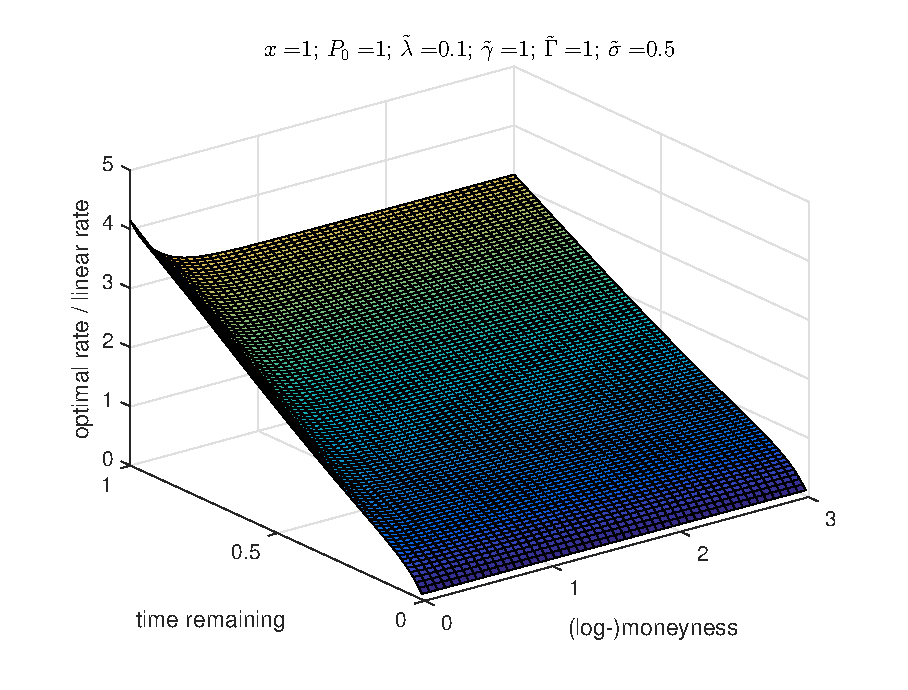
\includegraphics[]{ABM_lin.eps}
%\caption{Optimal liquidation VS straight line liquidation (Arithmetic Brownian motion case)}
%\label{fig:ABM_lin}
%\end{figure}

%\begin{figure}
%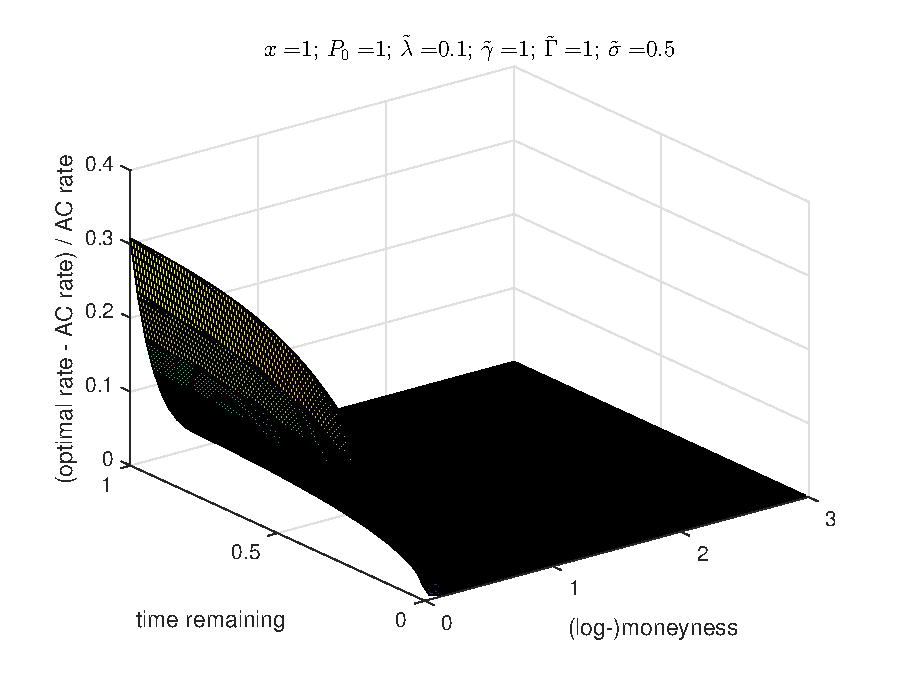
\includegraphics[]{ABM_AC.eps}
%\caption{Optimal liquidation VS Almgren-Chriss liquidation (Arithmetic Brownian motion case)}
%\label{fig:ABM_lin}
%\end{figure}

%\begin{figure}
%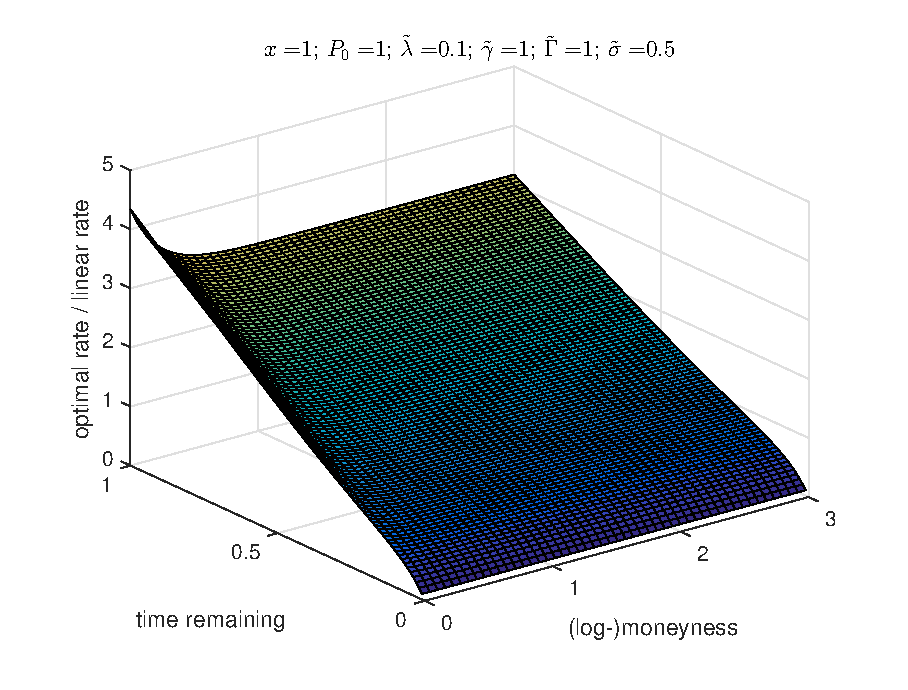
\includegraphics[]{GBM_lin.eps}
%\caption{Optimal liquidation VS straight line liquidation (Geometric Brownian motion case)}
%\label{fig:ABM_lin}
%\end{figure}

%\begin{figure}
%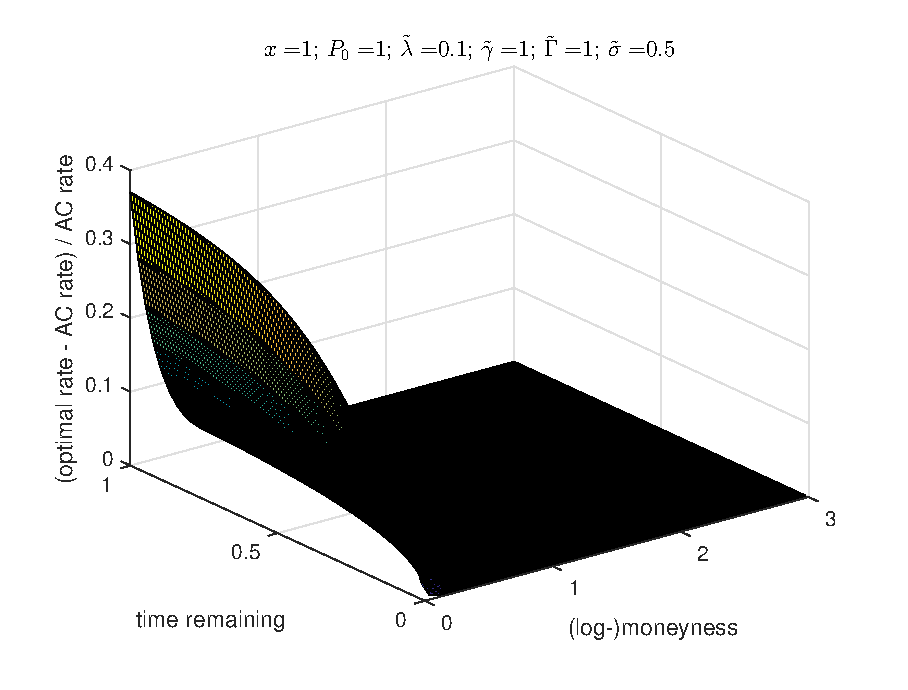
\includegraphics[]{GBM_AC.eps}
%\caption{Optimal liquidation VS Almgren-Chriss liquidation (Geometric Brownian motion case)}
%\label{fig:ABM_lin}
%\end{figure}

% In particular, at time $t=0$ and upon assuming that $P:=P_0=S_0$, this yields
% \begin{align*}
%  \ts u_0^* &\ts= \frac{G'(T)}{G(T)} x + \frac{P}{2\lambda}\int_t^T  \frac{G(T-s)}{G(T)} \bigl[ \frac{1}{\sqrt{s}}p\bigl(f(P,P,s,0)\bigr)+\frac{1}{2}\mathcal N\bigl(f(P,P,s,0)\bigr)\bigr] \de s\\
%            &\ts= \bigl[2\lambda\beta\cosh(\beta T)+2\Gamma\sinh(\beta T)\bigr]^{-1}\\
% 					 &\ts\hspace{1.5cm}\times\Bigl[ 2\bigl[\Gamma\beta\cosh(\beta T)+\gamma\sinh(\beta T)\bigr] x\\
% 					 &\ts\hspace{2.5cm}+ P\int_0^T  \bigl[\beta\cosh(\beta (T-s))+\lambda^{-1}\Gamma\sinh(\beta (T-s))\bigr] \bigl[ \frac{\sigma}{\sqrt{s}}p\bigl(\frac{\sigma\sqrt{s}}{2} - \frac{1}{\sigma\sqrt{s}}\log\left(\frac{c}{P}\right)\bigr)\\
% 					 &\ts\hspace{9.5cm}+\frac{1}{2}\sigma^2 \mathcal N\bigl(\frac{\sigma\sqrt{s}}{2} - \frac{1}{\sigma\sqrt{s}}\log\left(\frac{c}{P}\right)\bigr)\bigr] \de s\Bigr].
% \end{align*}


% {\color{red}
% For the sake of numerical implementation (e.g. in Matlab), we express our results as follows.
% \begin{multline*}
% \ts \de_s L_s(t) = S_t\sigma^2 \Bigl[p\left(\log\left(\frac{c-P_t}{S_t}+1 \right); \frac{1}{2}\sigma^2(s-t), \sigma^2(s-t)\right)\\
%    \ts + \frac{1}{2}\left(1-\mathcal{N}\left(\log\left(\frac{c-P_t}{S_t}+1 \right); \frac{1}{2}\sigma^2(s-t), \sigma^2(s-t)\right)\right)\Bigr] \de s,
% \end{multline*}
% where $p(\cdot;\mu,\Sigma)$ and $\mathcal{N}(\cdot;\mu, \Sigma)$ are respectively the probability density function and the cumulative distribution function of a normal random variable with mean $\mu\in\mathbb{R}$ and variance $\Sigma>0$.

% With $\tau$ and $u^M$ as in the case of arithmetic Brownian motion, and further introducing the ``log-moneyness'' variable $l:=\log\left(\frac{c-P_t}{S_t}+1\right)$, we have
% \begin{align*}
% \ts u^\ast_t = u^M_t + \frac{S_t\sigma^2}{2\lambda}\int_0^\tau \frac{G(\tau-s)}{G(\tau)}\left[p(l;\frac{1}{2}\sigma^2 s, \sigma^2 s)+\frac{1}{2}(1-\mathcal{N}(l;\frac{1}{2}\sigma^2 s, \sigma^2 s))\right] \de s.
% \end{align*}

%\subsection{Geometric Brownian motion}
%Now suppose that $S$ is a standard geometric Brownian motion, i.e. $S_t:=\mathcal{E}(B)_t = \exp\left(B_t-\frac{1}{2}t\right)$ in which $B$ is a standard Brownian motion. We would like to compute $\P_t(\tau_t(y)\le s) = \P^{0,S_t}(\tau_0(y)\le s-t)$ for $y>M_t$.
%
%For simplicity, we will compute $\P^{0,x}(\tau_0(y)\le \theta)$ for $y>x$. Define $\tilde{B}_t:=B_t-\frac{1}{2}t$ and $Z_t:=\exp\left(-\frac{1}{2}\tilde{B}_t-\frac{1}{8}t\right)$. Set $\tilde\tau(z):=\inf\{t\in[0,\infty] : \tilde{B}_t = z\}$. Let $\tilde\P$ be such that $\frac{d\P}{d\tilde\P}=Z_\theta$, then by Girsanov's theorem, $\{\tilde{B}_t\}_{t\in[0,\theta]}$ is a Brownian motion under $\tilde\P$. Thus, with knowledge of the first hitting time of a standard Brownian motion,
%\begin{align*}
%& \P^{0,x}(\tau_0(y)\le \theta) = \P(\tilde\tau(\log(y/x)) \le \theta) = \tilde\E\left[Z_\theta \I_{\{\tilde\tau(\log(y/x))\le \theta\}}\right] = \tilde\E\left[Z_{\tilde\tau(\log(y/x))} \I_{\{\tilde\tau(\log(y/x))\le \theta\}}\right] \\
%=& \tilde\E\left[\exp\left(-\frac{1}{2}\log(y/x)-\frac{1}{8}\tilde\tau(\log(y/x))\right) \I_{\{\tilde\tau(\log(y/x))\le \theta\}}\right] = \int_0^\theta (y/x)^{-1/2}e^{-t/8} d_t\tilde\P(\tilde\tau(\log(y/x)) \le t) \\
%=& \int_0^\theta (y/x)^{-1/2}e^{-t/8} d_t\left(2\tilde\P(\tilde{B}_t>\log(y/x))\right) = \int_0^\theta (y/x)^{-1/2}e^{-t/8} d_t\left(2\int_{\log(y/x)}^\infty p(t,z) dz\right) \\
%=& \int_0^\theta (y/x)^{-1/2}e^{-t/8} \left(\int_{\log(y/x)}^\infty 2\partial_t p(t,z) dz\right) dt = \int_0^\theta (y/x)^{-1/2}e^{-t/8} \left(\int_{\log(y/x)}^\infty \partial^2_z p(t,z) dz\right) dt \\
%=& -\int_0^\theta (y/x)^{-1/2}e^{-t/8} \partial_z p(t,\log(y/x)) dt, \quad \textrm{ where } p(t,z):=(2\pi t)^{-1/2}\exp\left(-\frac{z^2}{2t}\right).
%\end{align*}
%Therefore, let $z:=\log(y/x)$ we have
%\begin{align*}
%& \int_K^\infty \P^{0,x}(\tau_0(y)\le \theta) dy = -\int_{\log(K/x)}^\infty \int_0^\theta e^{-z/2} e^{-t/8} \partial_z p(t,z) dt d(xe^{z}) = -x \int_0^\theta e^{-t/8} \int_{\log(K/x)}^\infty e^{z/2} \partial_z p(t,z)) dz dt \\
%=& x \int_0^\theta e^{-t/8} \left[(K/x)^{1/2} p(t,\log(K/x)) + \int_{\log(K/x)}^\infty \frac{1}{2}e^{z/2}p(t,z) dz\right] dt \\
%=& x \int_0^\theta \left[p(t,\log(K/x)-t/2) + \frac{1}{2}\int_{\log(K/x)}^\infty p(t,z-t/2) dz\right] dt.
%\end{align*}
%With $x=S_t, K=c\vee M_t=(c\vee M_t -c - S_t) + c + S_t =c-P_t+S_t$, and $\theta=s-t$, we obtain
%\begin{align*}
%& L_s(t)=S_t \int_0^{s-t} \left[ p\left(\tau,\log\left(\frac{c-P_t}{S_t}+1\right)-\tau/2 \right)+\frac{1}{2}\int_{\log\left(\frac{c-P_t}{S_t}+1\right)}^\infty p(\tau,z-\tau/2)dz \right] d\tau \\
%\Rightarrow & d_s L_s(t) = S_t\left[ p\left(s-t,\log\left(\frac{c-P_t}{S_t}+1\right)-\frac{s-t}{2} \right)+\frac{1}{2}\int_{\log\left(\frac{c-P_t}{S_t}+1\right)}^\infty p\left(s-t,z-\frac{s-t}{2}\right)dz \right] ds.
%\end{align*}
%In short, we also have an explicit formula for the optimal selling rate if $S$ is a geometric Brownian motion. 

%\subsection{It\^o Diffusion}
%If $S$ is a diffusion given by the stochastic differential equation (SDE) $dS_t = \sigma(t,S_t) dB_t$, where $\sigma$ is uniformly Lipschitz in space and $B$ is a standard Brownian motion (note that $S$ is a martingale), then the cumulative distribution function (CDF) of the first hitting time $\P^{t,x}(\tau_t(y)\le s)=:u(t,x;s,y)$ can be characterized as the bounded solution to the following linear heat equation:
%\begin{align*}
%\begin{cases}
%(\partial_t + \mathcal{L}^S)u = \partial_t u + \frac{1}{2}\sigma^2\partial^2_x u = 0, & t<s, x<y \\
%u(t,y;s,y)=1, & t<s \\
%u(s,x;s,y)=\I_{\{x=y\}}, & x<y
%\end{cases}.
%\end{align*}
%Then we can write $L_s(t) = \int_{c\vee M_t} u(t,B_t;s,y) dy$.
%
%Now that one has to solve a PDE for diffusive $S$, we can also directly obtain a PDE for $L_s(t)$. Set $u(t,x,y;s,K):=\E\left[(M_s-K)_+ \vert S_t=x, M_t=y\right]$, then $u$ solves the following linear heat equation:
%\begin{align*}
%\begin{cases}
%(\partial_t u + \mathcal{L}^S)u = \partial_t u + \frac{1}{2}\sigma^2\partial^2_x u = 0, & t<s, x<y \\
%\partial_y u(t,y,y;s,K) = 0, & t<s \\
%u(s,x,y;s,K) = (y-K)_+, & x<y
%\end{cases}
%\end{align*}
%Then we can write $L_s(t) = u(t,B_t,M_t;s,c\vee M_t)$.

%\subsection{Price floor and model assumptions}
%Our proposition also applies to the case of liquidating a positive position of an asset in the presence of a price floor, and in particular, there is a unique optimal strategy absolutely continuous with respect to time. Formally, let $P=S+(f-M)_+$ be the asset price in which $S\in\mathcal{H}^1$ is a martingale and $M_t:=\inf_{u\in[0,t]}S_u$ is the running minimum. This is the dual case of an asset of price $-P$ and a price cap at $-f$. Thus, $P_t\ge f$ with equality iff $S_t=M_t\le f$, and $E_t P_s = P_t + \E_t[(f\wedge M_t-M_s)_+]$ from the beginning of this section. Therefore, one can solve the optimal liquidation problem with a price floor by pricing fixed-strike lookback puts. In the case of $S=B$, a standard Brownian motion, the optimal selling rate is
%\begin{align*}
%r^\ast_t &= -\frac{1}{2\lambda G(T-t)}\left(-2\lambda G'(T-t) X_t + \int_t^T G(T-s)p(s-t,P_t-f) ds\right) \\
%&= -\left[2\lambda\beta\cosh(\beta (T-t))+2\Gamma\sinh(\beta (T-t))\right]^{-1} \\
%& \cdot \left(- 2\left[\Gamma\beta\cosh(\beta (T-t))+\gamma\sinh(\beta (T-t))\right] X_t + \int_t^T \left[\beta\cosh(\beta (T-s))+\lambda^{-1}\Gamma\sinh(\beta (T-s))\right] \frac{\exp{\left(-\frac{(P_t-f)^2}{2(s-t)}\right)}}{\sqrt{2\pi(s-t)}} ds \right),
%\end{align*}
%Note that the sign of the integral term is flipped.
%
%However, it makes little economic sense to interpret $\lambda r_t$ as the temporary price impact of selling $r_t dt$ units of the asset at the price floor $f$, because by definition there should be no downward price impact at the floor. In this case, one could argue that it is a trading cost from commissions or exchange fees instead of temporary price impact, but in reality, these costs are usually proportional to the total shares traded or even decreasing in trading intensities. Therefore, we think that our model is not suitable for asset liquidation in the presence of a price floor.

% references
\bibliographystyle{plainnat}
\phantomsection
\addcontentsline{toc}{section}{\refname}
\bibliography{References}

\end{document}